% Informe de situación de f1-data-platform (29-30/09/2026)
% Compilar desde esta carpeta:  latexmk -xelatex -outdir=build informe.tex
% Los capítulos de capitulos/ se generan desde notas/ con md2tex.py (no editarlos a mano).
\documentclass[11pt,openany]{report}
% Preámbulo del informe de situación de f1-data-platform (compilar con XeLaTeX o latexmk -xelatex)
\usepackage[a4paper,margin=2.4cm,headheight=14pt]{geometry}
\usepackage{fontspec}
\usepackage[spanish,es-noshorthands,es-tabla]{babel}
\setmainfont{Libertinus Serif}
\setsansfont{Fira Sans}[Scale=MatchLowercase]
\setmonofont{Fira Mono}[Scale=0.86]
\usepackage{microtype}
\usepackage[dvipsnames,table]{xcolor}
\usepackage{graphicx}
\usepackage{booktabs,tabularx,longtable,array,multirow}
\usepackage{enumitem}
\setlist{itemsep=2pt,topsep=4pt}
\usepackage{csquotes}
\usepackage{fancyhdr}
\usepackage{titlesec}
\usepackage{caption}
\captionsetup{font=small,labelfont={bf,sf}}
\usepackage{listings}
\usepackage{tcolorbox}
\tcbuselibrary{skins,breakable}
\usepackage{tikz}
\usetikzlibrary{positioning,arrows.meta,shapes.geometric,shapes.multipart,fit,backgrounds,calc,matrix,chains}
\usepackage{pgfplots}
\pgfplotsset{compat=1.18}
\usepackage{amssymb,pifont}
\usepackage{fvextra}
\usepackage[colorlinks,urlcolor=oiblue!75!black,linkcolor=ink,citecolor=ink]{hyperref}
\usepackage{bookmark}

% Colores del proyecto (paleta Okabe-Ito + rojo F1)
\definecolor{f1red}{HTML}{C8102E}
\definecolor{ink}{HTML}{1F2330}
\definecolor{muted}{HTML}{5B6170}
\definecolor{bronze}{HTML}{A0652A}
\definecolor{silver}{HTML}{7C8691}
\definecolor{gold}{HTML}{B8901A}
\definecolor{oiblue}{HTML}{0072B2}
\definecolor{oiorange}{HTML}{E69F00}
\definecolor{oigreen}{HTML}{009E73}
\definecolor{oisky}{HTML}{56B4E9}
\definecolor{oiverm}{HTML}{D55E00}
\definecolor{oipurple}{HTML}{CC79A7}
\definecolor{codebg}{HTML}{F5F6F8}

\titleformat{\chapter}[display]{\sffamily\bfseries\huge\color{ink}}{\color{f1red}\large\MakeUppercase{\chaptertitlename}\ \thechapter}{4pt}{}
\titleformat{\section}{\sffamily\bfseries\Large\color{ink}}{\color{f1red}\thesection}{0.8em}{}
\titleformat{\subsection}{\sffamily\bfseries\large\color{ink}}{\color{muted}\thesubsection}{0.8em}{}
\titleformat{\subsubsection}{\sffamily\bfseries\normalsize\color{ink}}{}{0em}{}
\setcounter{secnumdepth}{2}
\setcounter{tocdepth}{2}

\pagestyle{fancy}
\fancyhf{}
\fancyhead[L]{\sffamily\small\color{muted}\leftmark}
\fancyhead[R]{\sffamily\small\color{muted}f1-data-platform · Informe de situación}
\fancyfoot[C]{\sffamily\small\thepage}
\renewcommand{\headrulewidth}{0.3pt}

\lstset{
  basicstyle=\ttfamily\small,
  backgroundcolor=\color{codebg},
  frame=none,
  breaklines=true,
  columns=fullflexible,
  keepspaces=true,
  showstringspaces=false,
  xleftmargin=6pt,
  framexleftmargin=6pt,
  aboveskip=8pt,
  belowskip=8pt,
  keywordstyle=\color{oiblue}\bfseries,
  commentstyle=\color{muted}\itshape,
  stringstyle=\color{oiverm},
  literate={á}{{\'a}}1 {é}{{\'e}}1 {í}{{\'i}}1 {ó}{{\'o}}1 {ú}{{\'u}}1 {ñ}{{\~n}}1 {Á}{{\'A}}1 {É}{{\'E}}1 {Í}{{\'I}}1 {Ó}{{\'O}}1 {Ú}{{\'U}}1 {Ñ}{{\~N}}1 {ü}{{\"u}}1 {«}{{\guillemotleft}}1 {»}{{\guillemotright}}1 {→}{{$\to$}}1 {×}{{$\times$}}1
}

% Cajas de resumen, recomendación y aviso
\newtcolorbox{resumen}[1][Resumen]{enhanced,breakable,colback=codebg,colframe=ink,boxrule=0.4pt,arc=2pt,
  fonttitle=\sffamily\bfseries,title={#1},left=8pt,right=8pt}
\newtcolorbox{recomendacion}[1][Recomendación]{enhanced,breakable,colback=oigreen!6,colframe=oigreen!70!black,boxrule=0.4pt,arc=2pt,
  fonttitle=\sffamily\bfseries,title={#1},left=8pt,right=8pt}
\newtcolorbox{aviso}[1][Atención]{enhanced,breakable,colback=oiorange!8,colframe=oiorange!80!black,boxrule=0.4pt,arc=2pt,
  fonttitle=\sffamily\bfseries,title={#1},left=8pt,right=8pt}

% Estilos TikZ comunes
\tikzset{
  caja/.style={draw=ink,rounded corners=2pt,align=center,font=\sffamily\small,inner sep=5pt,fill=white},
  capa/.style={draw=none,rounded corners=4pt,inner sep=8pt},
  flecha/.style={-{Stealth[length=2.4mm]},thick,color=ink!80},
  flechad/.style={-{Stealth[length=2.4mm]},thick,dashed,color=muted},
  etiqueta/.style={font=\sffamily\scriptsize,color=muted},
  tabla/.style={rectangle split,rectangle split parts=2,draw=ink,rounded corners=1pt,align=left,font=\sffamily\scriptsize,
    rectangle split part fill={#1,white},inner sep=3pt,text width=3.3cm},
}

\newcommand{\code}[1]{\texttt{\small\color{ink!85!oiblue}#1}}
\newcommand{\urltexto}[1]{\texttt{\footnotesize #1}}
\newcommand{\si}{\textcolor{oigreen!80!black}{\ding{51}}}
\newcommand{\no}{\textcolor{oiverm}{\ding{55}}}
\newcommand{\parcial}{\textcolor{oiorange}{\ding{108}}}
\newcommand{\nada}{\textcolor{muted}{\ding{109}}}

% Bloques de código de las notas (fvextra corta las líneas largas)
\DefineVerbatimEnvironment{codigo}{Verbatim}{breaklines,breakanywhere,fontsize=\footnotesize,
  frame=leftline,framerule=1.2pt,rulecolor=\color{oiblue!50},xleftmargin=8pt,framesep=6pt}
\DefineVerbatimEnvironment{diagramatexto}{Verbatim}{breaklines,breakanywhere,fontsize=\scriptsize,
  frame=single,rulecolor=\color{muted!50},framesep=5pt,label={\sffamily\scriptsize descripción del diagrama}}
\newenvironment{nota}{\begin{tcolorbox}[enhanced,breakable,colback=codebg,colframe=codebg,
  borderline west={2pt}{0pt}{muted},arc=0pt,left=8pt,right=6pt,top=3pt,bottom=3pt,fontupper=\small]}{\end{tcolorbox}}
\newcommand{\fich}[1]{\texttt{\small\color{oiblue!70!black}#1}}
\newcommand{\prio}[1]{\textsf{\small\bfseries #1}}
\setlength{\emergencystretch}{3em}
\counterwithout{figure}{chapter}


\hypersetup{pdftitle={f1-data-platform: informe de situación},pdfauthor={Antonio Sánchez de la Blanca Romero}}

\newcommand{\parte}[2]{\part{#1}\label{#2}}

\begin{document}

% ---------------------------------------------------------------- Portada
\begin{titlepage}
\thispagestyle{empty}
\begin{tikzpicture}[remember picture,overlay]
  \fill[ink] (current page.north west) rectangle ([yshift=-7.2cm]current page.north east);
  \fill[f1red] ([yshift=-7.2cm]current page.north west) rectangle ([yshift=-7.45cm]current page.north east);
  \node[anchor=north west,text=white,font=\sffamily\bfseries\fontsize{30}{34}\selectfont,align=left]
    at ([xshift=2.4cm,yshift=-2.3cm]current page.north west) {f1-data-platform};
  \node[anchor=north west,text=white!80!ink,font=\sffamily\Large,align=left]
    at ([xshift=2.4cm,yshift=-3.9cm]current page.north west) {Informe de situación del proyecto};
  \node[anchor=north west,text=white!65!ink,font=\sffamily\normalsize,align=left]
    at ([xshift=2.4cm,yshift=-4.8cm]current page.north west) {Datos, arquitectura, código y visualizaciones · antes de la fase 7};
\end{tikzpicture}
\vspace*{7.6cm}

{\sffamily\large
\begin{tabular}{@{}ll@{}}
\textcolor{muted}{Autor del proyecto} & Antonio Sánchez de la Blanca Romero \\
\textcolor{muted}{Origen} & TFG «Formula 1 Dashboard» (UCLM, 2024) \\
\textcolor{muted}{Fecha} & 29–30 de septiembre de 2026 \\
\textcolor{muted}{Versión de datos} & F1DB v2026.15.1 · FastF1 2018–2026 (ronda 15) \\
\textcolor{muted}{Repositorio} & \href{https://github.com/AntonioSchez32/f1-data-platform}{github.com/AntonioSchez32/f1-data-platform} \\
\textcolor{muted}{Web} & \href{https://f1-data-platform.vercel.app}{f1-data-platform.vercel.app} \\
\textcolor{muted}{API} & \href{https://f1-data-api-h7c7.onrender.com/docs}{f1-data-api-h7c7.onrender.com/docs} \\
\end{tabular}}

\vfill
{\small\color{muted}
Documento elaborado a partir de nueve investigaciones independientes (datos que faltan, fuentes
externas, carreras al sprint, arquitectura de datos, arquitectura de aplicación, alternativas de
arquitectura, revisión de código, gráficos de otras webs y evaluación de nuestros gráficos). Las
cifras proceden de consultas de solo lectura a \code{data/gold/f1.duckdb}, a la capa bronze y al
código del repositorio en el commit \code{cceddd3}. No se ha modificado código del proyecto.\par}
\end{titlepage}

\pagenumbering{roman}
\tableofcontents
\clearpage
\pagenumbering{arabic}

% ---------------------------------------------------------------- Cómo leer
\chapter*{Cómo leer este informe}
\addcontentsline{toc}{chapter}{Cómo leer este informe}
\markboth{Cómo leer este informe}{}

El informe responde a los cuatro encargos de la noche del 29 de septiembre y está pensado para
leerse en dos niveles:

\begin{itemize}
  \item \textbf{Nivel de decisión (unas 20 páginas).} El capítulo~\ref{cap:resumen} resume el estado
  del proyecto, los hallazgos más importantes, las decisiones que conviene tomar y una hoja de ruta
  consolidada. Cada parte empieza con una síntesis de dos o tres páginas con diagramas propios.
  \item \textbf{Nivel de detalle (el resto).} Tras cada síntesis van los capítulos de detalle, uno por
  investigación, con las consultas SQL, las tablas de cobertura, las fichas de cada fuente, el
  recorrido por el código y las URL consultadas. Son la base documental de las síntesis.
\end{itemize}

\begin{center}\small
\begin{tabular}{@{}p{0.34\linewidth}p{0.58\linewidth}@{}}
\toprule
\textbf{Encargo} & \textbf{Dónde está} \\
\midrule
1. Datos que faltan, cómo obtenerlos y contrastarlos; vueltas de sprint & Parte~\ref{parte:datos}: capítulos \ref{cap:huecos}, \ref{cap:fuentes} y \ref{cap:sprint} \\
2. Arquitectura y estructura del proyecto; alternativas & Parte~\ref{parte:arq}: capítulos \ref{cap:app} y \ref{cap:alternativas} \\
3. Arquitectura de datos, qué hace cada parte del código, mejoras & Parte~\ref{parte:datosarq}: capítulos \ref{cap:datos} y \ref{cap:codigo} \\
4. Gráficos y récords: evaluación de los nuestros e ideas nuevas & Parte~\ref{parte:graficos}: capítulos \ref{cap:propios} y \ref{cap:externos} \\
Hoja de ruta y preparación de la fase 7 & Capítulo~\ref{cap:hoja} \\
\bottomrule
\end{tabular}
\end{center}

\noindent Convenciones: \si{} disponible o correcto, \parcial{} parcial, \no{} no disponible,
\nada{} existe en la fuente pero no se expone. Esfuerzo: \textbf{S} horas, \textbf{M} uno o dos
días, \textbf{L} más de tres días. Los identificadores \code{H1}–\code{H7}, \code{M1}–\code{M11} y
\code{B1}–\code{B8} son los huecos de datos del capítulo~\ref{cap:huecos}; \code{P1}–\code{P26} son
las propuestas de gráficos del capítulo~\ref{cap:propios}.

% ================================================================ RESUMEN
\chapter{Resumen ejecutivo}\label{cap:resumen}

\section{El proyecto en una página}

La plataforma está \textbf{completa, desplegada y en verde}: el TFG de Power BI se ha convertido en
un sistema de datos automatizado que ingiere cuatro fuentes, las concilia con dbt en capas
bronze/silver/gold, publica cada semana una base DuckDB en una release de GitHub, la sirve con una
API FastAPI y la muestra en una web Next.js accesible y bilingüe que replica las once páginas del
informe original y añade telemetría, constructores y calidad de datos.

\begin{center}\small
\begin{tabularx}{\linewidth}{@{}l>{\raggedright\arraybackslash}X>{\raggedright\arraybackslash}p{0.23\linewidth}@{}}
\toprule
\textbf{Componente} & \textbf{Qué hay} & \textbf{Estado} \\
\midrule
Ingesta (bronze) & F1DB v2026.15.1 (31 tablas), FastF1 (187 carreras 2018–2026 y telemetría de 63), Ergast 2022 (535\,748 vueltas), CSV de formula1db.com del TFG (1\,252\,550 vueltas); CLI \code{f1-ingest} idempotente & \si{} funciona; solo sesiones R y Q de FastF1 \\
Transformación (dbt) & 54 modelos (20 staging, 10 intermediate, 17 marts, 7 de calidad), 3 seeds, 3 macros, 50 tests; \code{dbt build} en 22\,s & \si{} todo pasa; 40 comprobaciones QA: 23 PASS, 17 INFO, 0 FAIL \\
Modelo gold & 5 dimensiones, 8 hechos, 4 agregados (TFG: 5 dimensiones y 6 hechos) & \si{} \\
API & FastAPI, 28 endpoints GET, DuckDB de solo lectura con cambio de versión en caliente, ETag por versión de datos; 30 pruebas & \si{} <\,60\,ms por endpoint; \parcial{} arranque en frío de Render \\
Web & Next.js 16, 16 páginas × 2 idiomas, 17 gráficos, 23 componentes; Playwright + axe (WCAG 2.2 AA), 38 pruebas & \si{} todas pasan también en producción \\
CI/CD & \code{ci.yml} (Python, dbt, imagen Docker, web) y \code{pipeline.yml} (lunes 06:00 UTC) & \si{} verde; \parcial{} acciones en Node 20 \\
Despliegue & Render (API, Frankfurt, free) + Vercel (web) + GitHub Releases (datos); coste 0\,€ & \si{}; \parcial{} Vercel ejecuta en Washington \\
\bottomrule
\end{tabularx}
\end{center}

\section{Doce hallazgos que importan}

\begin{enumerate}
  \item \textbf{Lo esencial está completo de 1950 a 2026}: resultados, parrillas, clasificación y
  campeonatos de las 1\,164 carreras. Los huecos están \emph{dentro} de cada carrera y crecen hacia
  atrás en el tiempo: hay posiciones vuelta a vuelta en todas, pero tiempos por vuelta solo desde
  1990 (cap.~\ref{cap:huecos}).
  \item \textbf{Las vueltas de sprint se pueden recuperar ya.} FastF1 tiene las 11\,319 vueltas
  oficiales de los 29 sprints (2021–2026) sin huecos; la vuelta~1, que FastF1 no cronometra, se
  reconstruye exactamente con el tiempo total de F1DB. Versión mínima: unos 4 días
  (cap.~\ref{cap:sprint}).
  \item \textbf{Hay un error visible en los sprints}: \code{dim\_race.has\_sprint} es falso en los
  12 sprints de 2021–2023, y la web los oculta aunque sus resultados están cargados. Se arregla en
  minutos derivándolo de \code{SPRINT\_RACE\_RESULT}.
  \item \textbf{Las banderas rojas caen una vuelta antes.} En 22 carreras la vuelta que contiene la
  suspensión (20–130 minutos) no está marcada; es el caso de São Paulo 2024 que obligó a filtrar
  vueltas lentas en la web. No hay ninguna bandera roja marcada en 2025.
  \item \textbf{2025–2026 dependen de una sola fuente} (FastF1): 734 vueltas sin tiempo (570
  recuperables sumando sectores), 436 con compuesto \code{NAN}/\code{NONE} y ningún compuesto
  Pirelli real (C1–C6) desde 2024. \textbf{Jolpica}, sucesor de Ergast y con el mismo esquema que ya
  cargamos, daría la segunda fuente con 1–2 días de trabajo (cap.~\ref{cap:fuentes}).
  \item \textbf{Tenemos más datos de los que mostramos}: F1DB trae libres desde 1986, warm-up,
  preclasificación, las clasificaciones de 1980–2005, la vuelta rápida de cada piloto y el piloto
  del día; FastF1 ofrece meteorología y mensajes de dirección de carrera con solo activar dos
  parámetros.
  \item \textbf{Antes de 1996 no existe ninguna fuente abierta de tiempos por vuelta} con la que
  contrastar el CSV de formula1db.com. Queda como limitación documentada; la única vía de validación
  interna es \code{f1resultsdatabase} (con riesgo de licencia).
  \item \textbf{La arquitectura es adecuada y no hay que reescribirla.} Las guías de referencia (dbt
  Labs, uv, Next.js) respaldan las decisiones tomadas. El punto débil es el \emph{serving}: una API
  que se duerme a los 15 minutos para servir datos que solo cambian los lunes
  (cap.~\ref{cap:alternativas}).
  \item \textbf{La web no aprovecha ninguna caché de página}: todas se generan en cada visita, las
  funciones de Vercel se ejecutan en Washington mientras la API está en Frankfurt, y la portada tarda
  1,3–1,5\,s en empezar a responder (cap.~\ref{cap:app}).
  \item \textbf{Hay dos errores de datos que se ven en la web}: 85 vueltas duplicadas de coches
  compartidos en los años 50–60 (la pestaña de neumáticos las superpone) y abreviaturas de piloto que
  chocan en la misma carrera (Michael y Ralf Schumacher, ambos «SCH») (cap.~\ref{cap:codigo}).
  \item \textbf{La operación es frágil en tres puntos}: la release \code{data-latest} se sobrescribe
  cada semana y es la única copia en la nube del bronze de formula1db.com y Ergast; no hay prueba de
  humo antes de publicar; y el repositorio no tiene \code{LICENSE} ni atribuciones, que F1DB exige.
  \item \textbf{Las visualizaciones replican bien el TFG, pero se solapan y dejan preguntas sin
  responder.} Faltan el \emph{race trace} (diferencia con el líder vuelta a vuelta), la página de
  circuito, un comparador libre de pilotos y el momento en que se decidió el título. Hay tres
  gráficos que dicen lo mismo sobre los compañeros, y varios errores de lectura concretos
  (cap.~\ref{cap:propios}).
\end{enumerate}

\section{Decisiones que conviene tomar}

\begin{center}\small
\begin{longtable}{@{}>{\raggedright\arraybackslash}p{0.2\linewidth}>{\raggedright\arraybackslash}p{0.34\linewidth}>{\raggedright\arraybackslash}p{0.38\linewidth}@{}}
\toprule
\textbf{Decisión} & \textbf{Opciones} & \textbf{Recomendación} \\
\midrule\endhead
\bottomrule\endlastfoot
Licencia de los datos y del código & (a) MIT/Apache para el código y CC BY 4.0 para los datos derivados de F1DB; (b) además integrar Jolpica/OpenF1, que obliga a publicar lo derivado como CC BY-NC-SA & (a) ya. Integrar Jolpica y OpenF1 solo si se acepta la cláusula no comercial para los datos (el proyecto no es comercial, así que es asumible) \\
Vueltas de sprint & (a) versión mínima solo FastF1 (\textasciitilde4 días); (b) completa con validación Jolpica/OpenF1 y selector en la web (6–8,5 días); (c) aplazar & (b), empezando por (a). Antes, el arreglo de \code{has\_sprint} (minutos) \\
Segunda fuente para 2023–2026 & Jolpica (volcado CSV semanal) u OpenF1 (API, 30 peticiones/min) & Jolpica: mismo esquema que Ergast, 1–2 días \\
Cómo servir los datos a la web & A: endurecer lo actual; B: «API estática» (JSON precalculados en GitHub Pages, la API queda como servicio público); C: Dagster + R2 + DuckLake & A ahora (2–3 días) y B después (1–2 semanas); C como línea futura \\
Región de Vercel & Mantener Washington (\code{iad1}) o fijar Frankfurt (\code{fra1}) & \code{fra1}: una línea en \code{vercel.json} \\
Navegación de la web & Mantener 7 pestañas de carrera o pasar a 5 (Resultado, Clasificación, Carrera, Ritmo, Estrategia) y añadir Circuitos, Comparar e Historia & Pasar a 5 pestañas; añadir Circuitos y Comparar por fases \\
Casos de numeración aplazados (1994, 2001) & Resolverlos ahora o mantenerlos como pendientes documentados & Mantenerlos aplazados; no bloquean nada \\
Orden relativo con la fase 7 & Empezar la analítica ya o preparar antes los datos que necesita & Preparar antes meteorología, compuesto Cx y vueltas limpias (1–2 semanas), porque la degradación los necesita \\
\end{longtable}
\end{center}

\section{Hoja de ruta consolidada}\label{sec:hoja-resumen}

La tabla combina las propuestas de las nueve investigaciones, ordenadas por valor y esfuerzo. El
capítulo~\ref{cap:hoja} la desarrolla por iteraciones.

\begin{center}\small
\begin{longtable}{@{}>{\raggedright\arraybackslash}p{0.08\linewidth}>{\raggedright\arraybackslash}p{0.55\linewidth}>{\raggedright\arraybackslash}p{0.12\linewidth}>{\raggedright\arraybackslash}p{0.17\linewidth}@{}}
\toprule
\textbf{Iter.} & \textbf{Trabajo} & \textbf{Esfuerzo} & \textbf{Origen} \\
\midrule\endhead
\bottomrule\endlastfoot
1 & Arreglos rápidos de datos: \code{has\_sprint}, bandera roja en la vuelta correcta, tiempo desde sectores en 2025–26, \code{NAN}/\code{NONE} como nulo, tipos \code{HUGEINT}, tabla huérfana & 1 día & cap. \ref{cap:huecos}, \ref{cap:datos} \\
1 & Higiene: \code{LICENSE} y atribuciones, Dependabot, acciones fijadas a SHA y fuera de Node 20, cabeceras de seguridad, \code{fetch} con timeout, ruff alineado, región \code{fra1} & 1–2 días & cap. \ref{cap:codigo}, \ref{cap:app} \\
1 & Robustez de datos: releases fechadas e inmutables, copia del bronze estático, prueba de humo antes de publicar, arranque de la API con la última copia & 1–2 días & cap. \ref{cap:codigo}, \ref{cap:alternativas} \\
2 & Correcciones visibles: coches compartidos (\code{driver\_number} en la API), abreviaturas únicas, errores de lectura de los gráficos (referencia de clasificación, ejes de temporadas, Ferrari 1950–57, etiquetas solapadas, formato de miles) & 2–3 días & cap. \ref{cap:codigo}, \ref{cap:propios} \\
2 & Pruebas: unit tests de dbt para \code{int\_laptimes} e \code{int\_lap\_numbering}; tests de clave en paradas, standings, agregados y telemetría & 2 días & cap. \ref{cap:datos}, \ref{cap:codigo} \\
3 & Datos nuevos: FastF1 ampliado (sprint, meteo, dirección de carrera, libres), Jolpica como segunda fuente, eventos históricos SC/VSC/rojas como seed & 4–6 días & cap. \ref{cap:fuentes}, \ref{cap:sprint} \\
3 & Vueltas de sprint extremo a extremo (dbt, API \code{?session=sprint}, selector en la web) & 3–4 días & cap. \ref{cap:sprint} \\
4 & Gráficos de mayor valor: race trace, franjas SC/VSC, matriz de resultados de temporada, récords ampliados, eliminación matemática, pestañas 7\,→\,5 & 1–2 semanas & cap. \ref{cap:propios}, \ref{cap:externos} \\
5 & Arquitectura B: exportación estática de la API a GitHub Pages y revalidación bajo demanda & 1–2 semanas & cap. \ref{cap:alternativas} \\
6 & Fase 7: degradación de neumáticos, predicción de resultados, estilos de pilotaje & — & plan original \\
\end{longtable}
\end{center}

% ================================================================ PARTE I
\parte{Datos: qué falta, dónde conseguirlo y sprints}{parte:datos}

\chapter*{Síntesis de la parte I}
\addcontentsline{toc}{chapter}{Síntesis de la parte I}
\markboth{Síntesis de la parte I}{}

\section*{Qué cubrimos hoy}

La figura~\ref{fig:cobertura} resume la cobertura temporal de cada tipo de dato en la capa gold. El
patrón es claro: lo agregado por carrera está completo desde 1950, y el detalle por vuelta aparece
por capas a medida que avanzan las fuentes: posiciones desde 1950 (formula1db.com), tiempos desde
1990, paradas desde 1994, compuesto desde 2011 y todo lo demás desde 2018 con FastF1.

\begin{figure}[ht]
\centering
\begin{tikzpicture}[x=0.148cm,y=0.5cm,font=\sffamily\scriptsize]
  % eje de años 1950-2026 -> x = año-1950
  \foreach \a in {1950,1960,...,2020}{
    \draw[muted!30] ({\a-1950},0.4) -- ({\a-1950},-15.6);
    \node[muted,anchor=south] at ({\a-1950},0.4) {\a};
  }
  \node[muted,anchor=south] at (76,0.4) {2026};
  \newcommand{\fila}[5]{% #1 y, #2 etiqueta, #3 desde, #4 hasta, #5 color
    \node[anchor=east,text width=3.5cm,align=right] at (-1,-#1) {#2};
    \fill[#5,rounded corners=1pt] ({#3-1950},-#1-0.32) rectangle ({#4-1950+1},-#1+0.32);}
  \newcommand{\tramo}[4]{\fill[#4,rounded corners=1pt] ({#2-1950},-#1-0.32) rectangle ({#3-1950+1},-#1+0.32);}
  \fila{1}{Resultados, parrilla, campeonatos}{1950}{2026}{oiblue}
  \fila{2}{Clasificación (mejor tiempo)}{1950}{2026}{oiblue}
  \fila{3}{Q1/Q2/Q3}{2006}{2026}{oiblue}
  \fila{4}{Posición vuelta a vuelta}{1950}{2026}{oiblue}
  \tramo{4}{1950}{1959}{oisky}
  \fila{5}{Tiempo por vuelta}{1990}{2026}{oiblue}
  \tramo{5}{1990}{1995}{oisky}
  \fila{6}{Paradas (tiempo en pit lane)}{1994}{2026}{oiblue}
  \fila{7}{Compuesto por vuelta}{2011}{2026}{oiblue}
  \tramo{7}{2024}{2026}{oisky}
  \fila{8}{Stints, sectores, speed trap}{2018}{2026}{oiblue}
  \fila{9}{Safety car / VSC por vuelta}{1993}{2026}{oiblue}
  \fila{10}{Bandera roja por vuelta}{2007}{2026}{oisky}
  \fila{11}{Telemetría (vuelta de clasif.)}{2024}{2026}{oiblue}
  \fila{12}{Resultados de sprint}{2021}{2026}{oiblue}
  \node[anchor=east,text width=3.5cm,align=right] at (-1,-13) {Vueltas de sprint};
  \fill[oiorange!70,rounded corners=1pt] (71,-13.32) rectangle (77,-12.68);
  \node[anchor=east,text width=3.5cm,align=right] at (-1,-14) {Libres, warm-up, preclasif.};
  \fill[muted!35,rounded corners=1pt] (36,-14.32) rectangle (77,-13.68);
  \node[anchor=east,text width=3.5cm,align=right] at (-1,-15) {Meteo, dirección de carrera};
  \fill[oiorange!70,rounded corners=1pt] (68,-15.32) rectangle (77,-14.68);
  % leyenda
  \begin{scope}[shift={(0,-17)}]
    \fill[oiblue] (0,0) rectangle (2,0.5); \node[anchor=west] at (2.3,0.25) {en gold, completo};
    \fill[oisky] (38,0) rectangle (40,0.5); \node[anchor=west] at (40.3,0.25) {parcial o con problemas};
    \fill[oiorange!70] (0,-1.2) rectangle (2,-0.7); \node[anchor=west] at (2.3,-0.95) {disponible en FastF1, no cargado};
    \fill[muted!35] (38,-1.2) rectangle (40,-0.7); \node[anchor=west] at (40.3,-0.95) {en F1DB, sin exponer};
  \end{scope}
\end{tikzpicture}
\caption{Cobertura temporal de la capa gold por tipo de dato (datos del 28/09/2026). Tramos claros:
posiciones de los años 50 con un 43,6\,\% de «?», tiempos 1990–1995 sin segunda fuente, compuesto
sin C1–C6 desde 2024 y banderas rojas mal situadas.}
\label{fig:cobertura}
\end{figure}

\section*{Qué falta, por orden de importancia}

Los 26 huecos del inventario se agrupan en tres bloques con tratamiento distinto:

\begin{itemize}
  \item \textbf{Arreglos internos, sin fuentes nuevas} (H2, H3 en parte, H5, M11, B7, B8). La
  bandera roja se puede recolocar en la vuelta cuyo tiempo contiene la suspensión; los tiempos que
  faltan en 2025–26 salen sumando sectores; \code{has\_sprint} se deriva del resultado; los speed
  traps intermedios, el piloto del día y varias dimensiones de F1DB ya están en bronze.
  \item \textbf{Activar lo que ya tenemos a mano} (H1, M1–M4, M6, M8). FastF1 da vueltas de sprint,
  meteorología, mensajes de dirección de carrera, libres y telemetría de 2018–2023 cambiando
  parámetros del cargador existente. F1DB ya trae libres y las clasificaciones antiguas.
  \item \textbf{Fuentes nuevas} (H3, H4, H6, M5, M7, M9, M10 y los B1–B6 históricos). Aquí entran
  Jolpica, OpenF1, las nominaciones de Pirelli, los eventos históricos de Wikipedia/TracingInsights,
  Open-Meteo y, como último recurso para validar, \code{f1resultsdatabase}.
\end{itemize}

\section*{Dónde conseguirlo y cómo contrastarlo}

\begin{center}\small
\begin{tabularx}{\linewidth}{@{}l>{\raggedright\arraybackslash}X>{\raggedright\arraybackslash}p{0.18\linewidth}l@{}}
\toprule
\textbf{Fuente} & \textbf{Qué aporta (comprobado con peticiones reales)} & \textbf{Licencia} & \textbf{Esfuerzo} \\
\midrule
FastF1 ampliado & Sprint 2021+, meteo y dirección de carrera 2018+, libres, telemetría 2018–2023 & MIT (datos © F1) & 1–2 días \\
Jolpica-F1 & Tercera fuente de vueltas 1996+ y paradas con duración 2011+, al día en 2026; Q1–Q3 1994+ & CC BY-NC-SA 4.0 & 1–2 días \\
OpenF1 & 2023+: dirección de carrera, meteo, stints, adelantamientos, tiempo parado (2025+) & CC BY-NC-SA 4.0 & 2–3 días \\
TracingInsights RaceData & Safety car 1973+, banderas rojas 1950+, VSC 2015+ (de Wikipedia) & CC BY-SA & 1 día \\
Pirelli (prensa) & Compuestos nominados por GP desde 2011: validar neumáticos y obtener C1–C6 & © Pirelli (hechos) & 2 días \\
Open-Meteo ERA5 & Meteorología estimada 1940+ por coordenadas del circuito & CC BY 4.0 & 1 día \\
f1resultsdatabase & Posiciones por vuelta 1950+ y paradas 1983+ para validación interna & ODbL (origen dudoso) & 2–3 días \\
Documentos FIA & Evidencia para casos concretos (lap chart, history chart, pit stop summary) & no redistribuible & puntual \\
\bottomrule
\end{tabularx}
\end{center}

\begin{aviso}[Restricciones respetadas]
formula1db.com no se ha consultado: su \code{robots.txt} veta a los rastreadores y está tras
Cloudflare. statsf1.com rechaza clientes automáticos. No se ha descargado ningún volcado completo
(Jolpica, \code{f1resultsdatabase}) porque requiere tu permiso. Los PDF de la FIA se tratan solo como
evidencia.
\end{aviso}

\section*{Carreras al sprint: sí se puede}

La prueba con FastF1 cargó los 29 sprints disputados: 568 de los 590 pilotos cuadran vuelta a vuelta
con F1DB y el resto son casos explicables (vuelta de abandono, un DNS, una descalificación). El
diseño propuesto no toca el modelo de carreras largas:

\begin{itemize}
  \item bronze nuevo \code{fastf1/sprint\_laps} particionado igual que las vueltas de carrera;
  \item modelo \code{int\_sprint\_laptimes} separado, con un estado de validación \code{derived} para
  la vuelta 1 reconstruida;
  \item columna \code{session\_type} en \code{fact\_laptimes} y \code{fact\_pit\_lane\_passes}. Es el
  mayor riesgo: toda consulta que no filtre por sesión mezclaría sprint y carrera;
  \item parámetro \code{?session=sprint} en \code{/laps}, \code{/stints} y \code{/pit-lane-passes}, y
  un selector carrera/sprint en las pestañas de vueltas, neumáticos y ritmo.
\end{itemize}

\begin{recomendacion}
Primero la iteración~1 de arreglos internos (un día). Después, FastF1 ampliado y Jolpica, con lo
que en una semana quedan cubiertos los sprints, la dirección de carrera, la meteorología 2018+ y la
segunda fuente para 2023–2026. Los tiempos anteriores a 1990 se documentan como limitación.
\end{recomendacion}

\chapter{Inventario de los datos que faltan}\label{cap:huecos}
% Generado automáticamente desde notas/01_inventario_huecos.md con md2tex.py; no editar a mano.
Nota de trabajo para el informe de situación de \code{f1-\allowbreak{}data-\allowbreak{}platform} (29-09-2026). Base medida: \code{data/\allowbreak{}gold/\allowbreak{}f1.\allowbreak{}duckdb} construido el 28-09-2026 (F1DB \code{v2026.\allowbreak{}15.\allowbreak{}1}, publicada el 27-09-2026; 1 172 carreras en el calendario, 1 164 disputadas hasta Azerbaiyán 2026, ronda 15). Todas las cifras salen de consultas de solo lectura sobre esa base y sobre la capa bronze.

\medskip\noindent\textcolor{muted!40}{\rule{\linewidth}{0.3pt}}\medskip

\section{Resumen ejecutivo}

\begin{enumerate}
\item \textbf{Resultados, parrillas, clasificaciones y campeonatos están completos 1950→2026} (1 164 de 1 164 carreras). Lo que falta es el \textbf{detalle dentro de cada carrera}, y crece hacia atrás en el tiempo.
\item \textbf{Vueltas: todas las carreras tienen lap chart, pero no todas tienen tiempos.} Hay tiempo por vuelta solo desde 1990 (y no completo: faltan 4 carreras de 1990 y Hungría 1993). De 1950 a 1989 solo hay posiciones (y en los años 50 el 43,6 \% de ellas son desconocidas, «?» en formula1db.com). Excepción: Mónaco 1984 y Monza 1988 tienen tiempos.
\item \textbf{Faltan 3 223 vueltas de 116 pilotos} frente a las vueltas oficiales, más 39 de 11 pilotos sin ninguna vuelta; el 96 \% son de 1950–1959 (Indianápolis 1953–1955, relevos y coches compartidos). Desde 1970 solo faltan 28 vueltas sueltas (10 de ellas en Francia 1981).
\item \textbf{Validación de tiempos:} el 53,7 \% de las vueltas (682 058) son \code{single\_\allowbreak{}source}. Esto afecta a todo lo anterior a 1996 (Ergast empieza en 1996) y a todo 2025–2026, que solo tiene FastF1 (formula1db termina en Abu Dabi 2024).
\item \textbf{2025–2026 (FastF1 como única fuente):} 734 vueltas sin tiempo (570 de ellas tienen los tres sectores, así que el tiempo se puede calcular), 436 vueltas con compuesto \code{NAN}/\code{NONE} (354 en Miami 2025, 15 pilotos), y ninguna vuelta con compuesto Pirelli real (C1–C6).
\item \textbf{Banderas rojas mal marcadas.} Solo hay marcas desde 2007 (31 carreras). En 22 carreras (24 vueltas), la vuelta cuyo tiempo contiene la suspensión (20–130 min) no lleva \code{is\_\allowbreak{}red\_\allowbreak{}flag}. La marca, tanto de formula1db como de FastF1, cae en la vuelta en que se muestra la bandera, que es la anterior (São Paulo 2024, v. 33, es uno de estos casos). Además faltan todas las rojas anteriores a 2007 y Bélgica 2021.
\item \textbf{Paradas:} hay duración (tiempo en el pit lane) desde 1994, en 612 carreras. Faltan Brasil y Mónaco 1994 e Italia 1997. Desde 1990 hay entradas a boxes sin tipificar, y antes de 1990 no hay nada. En ninguna época está el tiempo parado.
\item \textbf{Neumáticos:} el compuesto está desde 2011 y los stints desde 2018 (con FastF1). No hay nada antes de 2011, y falta el compuesto Pirelli real en 2024–2026.
\item \textbf{Sesiones que F1DB ya tiene y el modelo no expone:} libres FP1–FP4 (1986+), warm-up (1984–2003), precalificación (1977–1992), clasificaciones de viernes y sábado (1980–2005), porcentaje del piloto del día y tiempo de parrilla.
\item \textbf{Sesiones que no carga ninguna fuente:} vueltas y paradas de las \textbf{carreras al sprint} (hay 29 sprints con resultado y 0 vueltas), vueltas de clasificación y libres, meteorología, mensajes de dirección de carrera y sanciones estructuradas. FastF1 las tiene todas desde 2018 (y los sprints desde 2021), pero el cargador las desactiva (\code{weather=\allowbreak{}False,\allowbreak{} messages=\allowbreak{}False}, solo sesiones R y Q).
\item \textbf{Telemetría:} solo la vuelta rápida de clasificación de cada piloto en 2024–2026 (63 carreras). No hay telemetría de 2018–2023 ni de carrera.
\item \textbf{Incoherencias de modelo:} \code{dim\_\allowbreak{}race.\allowbreak{}has\_\allowbreak{}sprint} vale falso en los 12 sprints de 2021–2023. FastF1 no tiene Italia 2018 en bronze, así que esa carrera no tiene stint, speed trap ni estado de pista. Queda una tabla huérfana, \code{silver.\allowbreak{}int\_\allowbreak{}formula1db\_\allowbreak{}laps\_\allowbreak{}validated}. Siguen abiertos los 3 casos de numeración de vueltas (San Marino y Japón 1994, Bélgica 2001).
\end{enumerate}

\medskip\noindent\textcolor{muted!40}{\rule{\linewidth}{0.3pt}}\medskip

\section{Metodología}

\subsection{Fuentes y qué cubre cada una (según \code{ingestion/\allowbreak{}} y \code{transform/\allowbreak{}})}

{\footnotesize\sloppy\setlength{\tabcolsep}{5pt}\renewcommand{\arraystretch}{1.15}
\begin{longtable}{@{}>{\raggedright\arraybackslash}p{0.157\dimexpr(\linewidth-50pt)\relax}>{\raggedright\arraybackslash}p{0.261\dimexpr(\linewidth-50pt)\relax}>{\raggedright\arraybackslash}p{0.261\dimexpr(\linewidth-50pt)\relax}>{\raggedright\arraybackslash}p{0.185\dimexpr(\linewidth-50pt)\relax}>{\raggedright\arraybackslash}p{0.136\dimexpr(\linewidth-50pt)\relax}@{}}
\toprule
\textbf{Fuente} & \textbf{Cargador} & \textbf{Qué aporta} & \textbf{Periodo} & \textbf{Estado} \\
\midrule\endhead
\bottomrule\endlastfoot
F1DB (SQLite, release GitHub) & \code{f1db\_\allowbreak{}loader.\allowbreak{}py} (todas las tablas) & Resultados, clasificación, parrillas, vuelta rápida, paradas, libres, campeonatos, dimensiones & 1950→actual & Semanal \\
formula1db.com (scraping del TFG) & \code{legacy\_\allowbreak{}loader.\allowbreak{}py} (solo \code{lap\_\allowbreak{}times} y \code{drivers}; \code{race\_\allowbreak{}entries} no está en bronze) & Vuelta a vuelta: posición, tiempo, diferencias, sectores, neumático, estado & 1950 → Abu Dabi 2024 & Congelado (web bloquea bots) \\
FastF1 & \code{fastf1\_\allowbreak{}loader.\allowbreak{}py}: sesión \textbf{R} (laps, results) y \textbf{Q} (results; telemetría opcional) & Vueltas 2025+; stint, vida del neumático, speed trap, estado de pista 2018+; Q1–Q3; telemetría de la vuelta rápida de clasificación & 2018→actual (telemetría 2024+) & Semanal (temporada en curso) \\
Ergast (volcado CSV oct-2022) & \code{ergast\_\allowbreak{}loader.\allowbreak{}py} & Solo validación de tiempos (1996–2022) y relleno N8 (0 vueltas) & 1996–2022 (vueltas), 2011–2022 (paradas) & Congelado \\
\end{longtable}}

Columnas de FastF1 que llegan a bronze y no se usan: \code{Speed\allowbreak{}I1}, \code{Speed\allowbreak{}I2}, \code{Speed\allowbreak{}FL}, \code{Fresh\allowbreak{}Tyre} (está en staging pero no en \code{fact\_\allowbreak{}laptimes}), \code{Deleted\allowbreak{}Reason}, \code{Pit\allowbreak{}In\allowbreak{}Time}/\code{Pit\allowbreak{}Out\allowbreak{}Time}, \code{Lap\allowbreak{}Start\allowbreak{}Date}, \code{Team\allowbreak{}Color} y \code{Headshot\allowbreak{}Url}. De F1DB no se usan \code{driver\_\allowbreak{}of\_\allowbreak{}the\_\allowbreak{}day\_\allowbreak{}percentage}, \code{starting\_\allowbreak{}grid\_\allowbreak{}position\_\allowbreak{}time}, \code{practice\_\allowbreak{}*} ni las tablas de chasis, motor, inscritos, trazados y relaciones familiares.

\subsection{Consultas principales}

Todas se lanzan desde \code{transform/\allowbreak{}} (las vistas de staging leen \code{.\allowbreak{}.\allowbreak{}/\allowbreak{}data/\allowbreak{}bronze/\allowbreak{}.\allowbreak{}.\allowbreak{}.\allowbreak{}}) con \code{duckdb.\allowbreak{}connect(\allowbreak{}'.\allowbreak{}.\allowbreak{}/\allowbreak{}data/\allowbreak{}gold/\allowbreak{}f1.\allowbreak{}duckdb',\allowbreak{} read\_\allowbreak{}only=\allowbreak{}True)}.

\textbf{Cobertura de vueltas frente a las oficiales por temporada.} Las vueltas oficiales salen de \code{RACE\_\allowbreak{}RESULT.\allowbreak{}race\_\allowbreak{}laps} (con correcciones).

\begin{codigo}
with off as (
  select race_id, driver_id, sum(race_laps) official_laps, bool_or(race_shared_car) shared
  from silver.int_race_data_corrected where session_type = 'RACE_RESULT' group by all),
lp as (select race_id, driver_id, count(distinct lap_number) rec from gold.fact_laptimes group by all)
select r.season, count(distinct r.race_id) races,
       sum(official_laps) oficiales, sum(least(coalesce(rec,0), official_laps)) cubiertas
from gold.dim_race r left join off using (race_id) left join lp using (race_id, driver_id)
where r.is_completed group by 1 order by 1;
\end{codigo}

\textbf{Estado por piloto y carrera.} Se usa el modelo \code{silver.\allowbreak{}int\_\allowbreak{}lap\_\allowbreak{}completeness}, que ya concilia las vueltas registradas con las oficiales:

\begin{codigo}
select r.season, r.round, r.grand_prix_name, c.status, count(*) pilotos, sum(missing_laps) faltan
from silver.int_lap_completeness c join gold.dim_race r using (race_id)
where status in ('missing_laps', 'no_laps', 'extra_laps') group by all order by 1, 2;
\end{codigo}

\textbf{Rellenado de cada campo de \code{fact\_\allowbreak{}laptimes} por temporada} (resultado en la §3.3):

\begin{codigo}
select r.season, count(*) vueltas,
  round(100.0*count(lap_time_ms)/count(*),1) tiempo, round(100.0*count(position)/count(*),1) pos,
  round(100.0*count(sector_1_ms)/count(*),1) s1, round(100.0*count(nullif(tyre_compound,''))/count(*),1) comp,
  round(100.0*count(tyre_compound_pirelli)/count(*),1) pirelli, round(100.0*count(stint)/count(*),1) stint,
  sum(is_pit_in_lap::int) boxes, sum(is_safety_car::int) sc, sum(is_red_flag::int) roja,
  round(100.0*count(speed_trap_kmh)/count(*),1) speed_trap
from gold.fact_laptimes join gold.dim_race r using (race_id) group by 1 order by 1;
\end{codigo}

\textbf{Suspensiones sin marca de bandera roja.} Una vuelta de más de 400 s que registran al menos 3 pilotos contiene la suspensión:

\begin{codigo}
select r.season, r.round, r.grand_prix_name, lap_number, count(*) n,
       median(lap_time_ms)/60000 min_mediana, bool_or(is_red_flag) marcada
from gold.fact_laptimes join gold.dim_race r using (race_id)
where lap_time_ms > 400000 group by all having count(*) >= 3 order by 1, 2, 4;
\end{codigo}

\textbf{Sesiones de F1DB por década} (incluidas las que no se exponen):

\begin{codigo}
select r.season//10*10 decada,
  count(distinct d.race_id) filter (where type = 'FREE_PRACTICE_1_RESULT') fp1, ...
from gold.dim_race r left join read_parquet('../data/bronze/f1db/race_data.parquet') d
  on r.race_id = d.race_id group by 1;
\end{codigo}

Además se consultaron \code{quality.\allowbreak{}qa\_\allowbreak{}summary}, \code{silver.\allowbreak{}int\_\allowbreak{}lap\_\allowbreak{}numbering}, \code{silver.\allowbreak{}int\_\allowbreak{}formula1db\_\allowbreak{}race\_\allowbreak{}alignment}, \code{gold.\allowbreak{}fact\_\allowbreak{}pit\_\allowbreak{}stops}, \code{gold.\allowbreak{}fact\_\allowbreak{}pit\_\allowbreak{}lane\_\allowbreak{}passes}, \code{gold.\allowbreak{}fact\_\allowbreak{}qualifying\_\allowbreak{}result}, \code{gold.\allowbreak{}fact\_\allowbreak{}race\_\allowbreak{}result}, \code{gold.\allowbreak{}fact\_\allowbreak{}quali\_\allowbreak{}telemetry} y el \code{Track\allowbreak{}Status} de bronze de FastF1.

\medskip\noindent\textcolor{muted!40}{\rule{\linewidth}{0.3pt}}\medskip

\section{Tablas de cobertura}

\subsection{Matriz de cobertura por tipo de dato}

\si{} completo · \parcial{} parcial · \no{} no hay · \nada{} la fuente existe pero no se expone en gold

{\scriptsize\sloppy\setlength{\tabcolsep}{4pt}\renewcommand{\arraystretch}{1.15}
\begin{longtable}{@{}>{\raggedright\arraybackslash}p{0.161\dimexpr(\linewidth-96pt)\relax}>{\raggedright\arraybackslash}p{0.089\dimexpr(\linewidth-96pt)\relax}>{\raggedright\arraybackslash}p{0.041\dimexpr(\linewidth-96pt)\relax}>{\raggedright\arraybackslash}p{0.028\dimexpr(\linewidth-96pt)\relax}>{\raggedright\arraybackslash}p{0.045\dimexpr(\linewidth-96pt)\relax}>{\raggedright\arraybackslash}p{0.112\dimexpr(\linewidth-96pt)\relax}>{\raggedright\arraybackslash}p{0.082\dimexpr(\linewidth-96pt)\relax}>{\raggedright\arraybackslash}p{0.045\dimexpr(\linewidth-96pt)\relax}>{\raggedright\arraybackslash}p{0.062\dimexpr(\linewidth-96pt)\relax}>{\raggedright\arraybackslash}p{0.101\dimexpr(\linewidth-96pt)\relax}>{\raggedright\arraybackslash}p{0.112\dimexpr(\linewidth-96pt)\relax}>{\raggedright\arraybackslash}p{0.123\dimexpr(\linewidth-96pt)\relax}@{}}
\toprule
\textbf{Dato} & \textbf{1950–59} & \textbf{60–69} & \textbf{70–79} & \textbf{80–89} & \textbf{90–95} & \textbf{96–2005} & \textbf{06–10} & \textbf{11–17} & \textbf{18–24} & \textbf{25–26} & \textbf{Origen} \\
\midrule\endhead
\bottomrule\endlastfoot
Resultado de carrera & \si{} & \si{} & \si{} & \si{} & \si{} & \si{} & \si{} & \si{} & \si{} & \si{} & F1DB \\
Parrilla & \si{} & \si{} & \si{} & \si{} & \si{} & \si{} & \si{} & \si{} & \si{} & \si{} & F1DB \\
Penalización de parrilla (texto) & \no{} & \no{} & \no{} & \no{} & \parcial{} & \parcial{} & \parcial{} & \si{} & \si{} & \si{} & F1DB (\nada{} solo en silver) \\
Clasificación: mejor tiempo & \si{} & \si{} & \si{} & \si{} & \si{} & \si{} & – & – & – & – & F1DB \\
Clasificación: Q1/Q2/Q3 & – & – & – & – & – & – & \si{} & \si{} & \si{} & \si{} & F1DB (+FastF1 QA) \\
Clasificaciones de viernes y sábado & \no{} & \no{} & \no{} & \nada{} & \nada{} & \nada{} (hasta 2002) & – & – & – & – & F1DB \code{QUALIFYING\_\allowbreak{}1/\allowbreak{}2\_\allowbreak{}RESULT} \\
Nº de vueltas de clasificación & \no{} & \no{} & \no{} & \no{} & \parcial{} (1994+) & \si{} & \si{} & \si{} & \si{} & \si{} & F1DB \\
Precalificación & – & – & \nada{} & \nada{} & \nada{} & – & – & – & – & – & F1DB (1977–1992) \\
Libres (mejor tiempo y vueltas) & \no{} & \no{} & \no{} & \nada{} (1986+) & \nada{} & \nada{} & \nada{} & \nada{} & \nada{} & \nada{} & F1DB \\
Warm-up & \no{} & \no{} & \no{} & \nada{} (1984+) & \nada{} & \nada{} (hasta 2003) & – & – & – & – & F1DB \\
Vuelta rápida de cada piloto & \parcial{} (solo la absoluta) & \parcial{} & \parcial{} & \parcial{} (74 \%) & \si{} & \si{} & \si{} & \si{} & \si{} & \si{} & F1DB \code{FASTEST\_\allowbreak{}LAP} (\nada{} solo QA) \\
Posición vuelta a vuelta & \parcial{} (56 \%) & \parcial{} (95 \%) & \si{} & \si{} & \si{} & \si{} & \si{} & \si{} & \si{} & \si{} & formula1db / FastF1 \\
Tiempo por vuelta & \no{} & \no{} & \no{} & \no{}* & \parcial{} (4 carreras sin tiempos) & \si{} & \si{} & \si{} & \si{} & \parcial{} (97,8–98,7 \%) & formula1db / FastF1 \\
Validación con otra fuente & \no{} & \no{} & \no{} & \no{} & \no{} & \si{} Ergast & \si{} & \si{} & \si{} Ergast+FastF1 & \no{} & — \\
Sectores & \no{} & \no{} & \no{} & \no{} & \no{} & \no{} & \no{} & \no{} & \si{} (\textasciitilde{}98 \%) & \si{} & formula1db 2018+ / FastF1 \\
Entradas y salidas de boxes por vuelta & \no{} & \no{} & \no{} & \no{} & \si{} & \si{} & \si{} & \si{} & \si{} & \si{} & formula1db / FastF1 \\
Paradas (vuelta y duración) & \no{} & \no{} & \no{} & \no{} & \parcial{} (1994–95) & \si{} & \si{} & \si{} & \si{} & \si{} & F1DB \\
Tiempo parado & \no{} & \no{} & \no{} & \no{} & \no{} & \no{} & \no{} & \no{} & \no{} & \no{} & — \\
Compuesto por vuelta & \no{} & \no{} & \no{} & \no{} & \no{} & \no{} & \no{} & \si{} & \si{} (C1–C5 solo 2019–23) & \parcial{} (sin Cx; Miami 2025 \code{NAN}) & formula1db / FastF1 \\
Vida del neumático & \no{} & \no{} & \no{} & \no{} & \no{} & \no{} & \no{} & \parcial{} (2014–15) & \si{} & \si{} & formula1db / FastF1 \\
Stint & \no{} & \no{} & \no{} & \no{} & \no{} & \no{} & \no{} & \no{} & \si{} (menos Italia 2018) & \si{} & FastF1 \\
Speed trap & \no{} & \no{} & \no{} & \no{} & \no{} & \no{} & \no{} & \no{} & \si{} (menos Italia 2018) & \si{} & FastF1 (I1, I2 y FL sin usar) \\
Amarilla / SC / VSC por vuelta & \no{} & \no{} & \no{} & \no{} & \parcial{} (SC 1993+) & \si{} (amarilla 1996+) & \si{} & \si{} (VSC 2015+) & \si{} & \si{} & formula1db / FastF1 \\
Bandera roja por vuelta & \no{} & \no{} & \no{} & \no{} & \no{} & \no{} & \parcial{} (2007+) & \parcial{} & \parcial{} (desfase de 1 vuelta) & \parcial{} & formula1db / FastF1 \\
Telemetría & \no{} & \no{} & \no{} & \no{} & \no{} & \no{} & \no{} & \no{} & \parcial{} (Q 2024) & \parcial{} (Q) & FastF1 \\
Meteorología & \no{} & \no{} & \no{} & \no{} & \no{} & \no{} & \no{} & \no{} & \no{} & \no{} & (FastF1 2018+, sin cargar) \\
Dirección de carrera y sanciones & \no{} & \no{} & \no{} & \no{} & \no{} & \no{} & \no{} & \no{} & \no{} & \no{} & (FastF1 2018+, sin cargar) \\
Sprint: resultado y parrilla & – & – & – & – & – & – & – & – & \si{} (2021+) & \si{} & F1DB \\
Sprint: clasificación SQ1–SQ3 & – & – & – & – & – & – & – & – & \si{} (2023+) & \si{} & F1DB \\
Sprint: vueltas, paradas y vuelta rápida & – & – & – & – & – & – & – & – & \no{} & \no{} & (FastF1 sesión S, sin cargar) \\
Piloto del día & – & – & – & – & – & – & – & \parcial{} (2016+) & \si{} & \si{} & F1DB (sin el porcentaje) \\
Hora de salida (UTC) & \no{} & \no{} & \no{} & \no{} & \no{} & \no{} & \no{} & \no{} & \parcial{} & \si{} & F1DB (71 carreras) \\
\end{longtable}}

\textbackslash{}* De 1950 a 1989 solo tienen tiempos Mónaco 1984 (396 vueltas), Monza 1988 (927) y 33 vueltas de Mónaco 1989.

\subsection{Vueltas oficiales cubiertas por década}

Vueltas oficiales = suma de \code{race\_\allowbreak{}laps} por piloto. Cubiertas = vueltas registradas dentro del rango oficial (\code{int\_\allowbreak{}lap\_\allowbreak{}completeness.\allowbreak{}recorded\_\allowbreak{}in\_\allowbreak{}range}, sin contar las que pasan de las oficiales). Parcial = al menos un piloto con \code{missing\_\allowbreak{}laps} o \code{no\_\allowbreak{}laps}. La última columna excluye los coches compartidos y los descalificados.

{\scriptsize\sloppy\setlength{\tabcolsep}{4pt}\renewcommand{\arraystretch}{1.15}
\begin{longtable}{@{}>{\raggedright\arraybackslash}p{0.067\dimexpr(\linewidth-72pt)\relax}>{\raggedright\arraybackslash}p{0.086\dimexpr(\linewidth-72pt)\relax}>{\raggedright\arraybackslash}p{0.095\dimexpr(\linewidth-72pt)\relax}>{\raggedright\arraybackslash}p{0.095\dimexpr(\linewidth-72pt)\relax}>{\raggedright\arraybackslash}p{0.113\dimexpr(\linewidth-72pt)\relax}>{\raggedright\arraybackslash}p{0.163\dimexpr(\linewidth-72pt)\relax}>{\raggedright\arraybackslash}p{0.095\dimexpr(\linewidth-72pt)\relax}>{\raggedright\arraybackslash}p{0.067\dimexpr(\linewidth-72pt)\relax}>{\raggedright\arraybackslash}p{0.219\dimexpr(\linewidth-72pt)\relax}@{}}
\toprule
\textbf{Década} & \textbf{Carreras} & \textbf{Completas} & \textbf{Parciales} & \textbf{Sin vueltas} & \textbf{Vueltas oficiales} & \textbf{Cubiertas} & \textbf{\%} & \textbf{\% sin compartidos ni DSQ} \\
\midrule\endhead
\bottomrule\endlastfoot
1950 & 84 & 44 & 40 & 0 & 108 257 & 104 650 & 96,67 & 97,01 \\
1960 & 100 & 89 & 11 & 0 & 92 875 & 92 700 & 99,81 & 99,89 \\
1970 & 144 & 142 & 2 & 0 & 157 646 & 157 641 & 100,00 & 100,00 \\
1980 & 156 & 151 & 5 & 0 & 166 476 & 166 446 & 99,98 & 99,98 \\
1990 & 162 & 161 & 1 & 0 & 174 640 & 174 639 & 100,00 & 100,00 \\
2000 & 174 & 174 & 0 & 0 & 182 660 & 182 660 & 100,00 & 100,00 \\
2010 & 198 & 198 & 0 & 0 & 226 213 & 226 213 & 100,00 & 100,00 \\
2020 & 146 & 146 & 0 & 0 & 160 245 & 160 244 & 100,00 & 100,00 \\
\end{longtable}}

Hay además vueltas registradas por encima de las oficiales: 1 027 de los Tyrrell descalificados en 1984 (F1DB les pone 0 vueltas), 7 716 de coches compartidos y vueltas de abandono de FastF1.

\textbf{Estado por piloto (\code{int\_\allowbreak{}lap\_\allowbreak{}completeness}, 25 752 pares carrera-piloto):}

{\footnotesize\sloppy\setlength{\tabcolsep}{5pt}\renewcommand{\arraystretch}{1.15}
\begin{longtable}{@{}>{\raggedright\arraybackslash}p{0.143\dimexpr(\linewidth-40pt)\relax}>{\raggedright\arraybackslash}p{0.091\dimexpr(\linewidth-40pt)\relax}>{\raggedright\arraybackslash}p{0.202\dimexpr(\linewidth-40pt)\relax}>{\raggedright\arraybackslash}p{0.563\dimexpr(\linewidth-40pt)\relax}@{}}
\toprule
\textbf{Estado} & \textbf{Pilotos} & \textbf{Vueltas que faltan} & \textbf{Comentario} \\
\midrule\endhead
\bottomrule\endlastfoot
ok & 25 339 & 0 &  \\
missing\_laps & 116 & 3 223 & 95 de ellos en los años 50 (3 097 vueltas) \\
no\_laps & 11 & 39 & Abandonos en la vuelta 1 no registrados (años 50–80) y Behra, Italia 1951 (29) \\
extra\_laps & 9 & 7 & Francia 1981 (numeración tras el relanzamiento), Marimón 1954, Daywalt 1954, Russo 1960, Trintignant 1951, Gasly GB 2024 (1 vuelta sin estar en el resultado) \\
shared\_car & 117 & 531 & Coche compartido: la fuente no separa las vueltas de cada piloto \\
disqualified & 160 & 19 & F1DB no computa sus vueltas \\
\end{longtable}}

\subsection{Rellenado de campos de \code{fact\_\allowbreak{}laptimes} (\% de vueltas con valor)}

{\scriptsize\sloppy\setlength{\tabcolsep}{4pt}\renewcommand{\arraystretch}{1.15}
\begin{longtable}{@{}>{\raggedright\arraybackslash}p{0.086\dimexpr(\linewidth-96pt)\relax}>{\raggedright\arraybackslash}p{0.069\dimexpr(\linewidth-96pt)\relax}>{\raggedright\arraybackslash}p{0.061\dimexpr(\linewidth-96pt)\relax}>{\raggedright\arraybackslash}p{0.078\dimexpr(\linewidth-96pt)\relax}>{\raggedright\arraybackslash}p{0.078\dimexpr(\linewidth-96pt)\relax}>{\raggedright\arraybackslash}p{0.086\dimexpr(\linewidth-96pt)\relax}>{\raggedright\arraybackslash}p{0.109\dimexpr(\linewidth-96pt)\relax}>{\raggedright\arraybackslash}p{0.078\dimexpr(\linewidth-96pt)\relax}>{\raggedright\arraybackslash}p{0.078\dimexpr(\linewidth-96pt)\relax}>{\raggedright\arraybackslash}p{0.061\dimexpr(\linewidth-96pt)\relax}>{\raggedright\arraybackslash}p{0.094\dimexpr(\linewidth-96pt)\relax}>{\raggedright\arraybackslash}p{0.125\dimexpr(\linewidth-96pt)\relax}@{}}
\toprule
\textbf{Periodo} & \textbf{Vueltas} & \textbf{Tiempo} & \textbf{Posición} & \textbf{Sectores} & \textbf{Compuesto} & \textbf{Pirelli (Cx)} & \textbf{Relativo} & \textbf{Vida} & \textbf{Stint} & \textbf{Speed trap} & \textbf{Boxes marcados} \\
\midrule\endhead
\bottomrule\endlastfoot
1950–1959 & 108 201 & 0 \% & 56 \% & 0 & 0 & 0 & 0 & 0 & 0 & 0 & 0 \\
1960–1969 & 92 874 & 0 \% & 95 \% & 0 & 0 & 0 & 0 & 0 & 0 & 0 & 0 \\
1970–1989 & 325 148 & 0,4 \% & 100 \% & 0 & 0 & 0 & 0 & 0 & 0 & 0 & 5 \\
1990 & 19 165 & 75,3 \% & 100 \% & 0 & 0 & 0 & 0 & 0 & 0 & 0 & 163 \\
1991–1995 & 91 880 & 98,5 \% & 100 \% & 0 & 0 & 0 & 0 & 0 & 0 & 0 & 2 109 \\
1996–2010 & 268 832 & 100 \% & 100 \% & 0 & 0 & 0 & 0 & 0 & 0 & 0 & 8 850 \\
2011–2017 & 157 786 & 100 \% & 100 \% & 0 & 100 \% & 100 \%† & 0–9 \% & 85–100 \% & 0 & 0 & 6 410 \\
2018 & 22 246 & 100 \% & 100 \% & 98,2 \% & 100 \% & 100 \%† & 0,1 \% & 100 \% & 94,5 \% & 95,8 \% & 557 \\
2019–2023 & 113 629 & 100 \% & 100 \% & \textasciitilde{}98 \% & 100 \% & 100 \% & 100 \% & 100 \% & \textasciitilde{}100 \% & \textasciitilde{}100 \% & 3 867 \\
2024 & 26 574 & 100 \% & 100 \% & 98,1 \% & 100 \% & \textbf{8,3 \%} & 100 \% & 100 \% & 100 \% & 100 \% & 844 \\
2025 & 26 689 & \textbf{98,7 \%} & 99,9 \% & 98,1 \% & 100 \%‡ & \textbf{6,0 \%} & 98,5 \% & 98,4 \% & 98,7 \% & 99,9 \% & 841 \\
2026 & 17 236 & \textbf{97,8 \%} & 99,8 \% & 97,5 \% & 100 \%‡ & \textbf{0,1 \%} & 99,9 \% & 99,7 \% & 100 \% & 99,8 \% & 625 \\
\end{longtable}}

† Hasta 2018 \code{tyre\_\allowbreak{}compound\_\allowbreak{}pirelli} es el nombre comercial (SOFT, SUPERSOFT…), no Cx. ‡ Incluye 354 vueltas \code{NAN} (Miami 2025, 15 pilotos), 57 \code{NONE} (Bélgica 2025) y 25 \code{NONE} (Hungría 2026). El \% de Pirelli en 2024–2026 corresponde solo a INTERMEDIATE/WET: \textbf{no hay compuesto Cx desde 2024} (formula1db 2024 y FastF1 dan HARD/MEDIUM/SOFT, y \code{int\_\allowbreak{}tyre\_\allowbreak{}compound\_\allowbreak{}mapping} solo cubre 2019–2023).

\subsection{Tiempo por vuelta: carreras sin tiempos o con tiempos parciales desde 1990}

{\footnotesize\sloppy\setlength{\tabcolsep}{5pt}\renewcommand{\arraystretch}{1.15}
\begin{longtable}{@{}>{\raggedright\arraybackslash}p{0.222\dimexpr(\linewidth-40pt)\relax}>{\raggedright\arraybackslash}p{0.091\dimexpr(\linewidth-40pt)\relax}>{\raggedright\arraybackslash}p{0.123\dimexpr(\linewidth-40pt)\relax}>{\raggedright\arraybackslash}p{0.564\dimexpr(\linewidth-40pt)\relax}@{}}
\toprule
\textbf{Carrera} & \textbf{Vueltas} & \textbf{Con tiempo} & \textbf{Comentario} \\
\midrule\endhead
\bottomrule\endlastfoot
EE. UU. 1990 (R1) & 1 341 & 0 & Solo lap chart \\
Brasil 1990 (R2) & 1 271 & 0 & Solo lap chart \\
San Marino 1990 (R3) & 1 026 & 0 & Solo lap chart \\
Mónaco 1990 (R4) & 1 084 & 0 & Solo lap chart \\
Alemania 1990 (R9) & 744 & 728 & 97,8 \% \\
Hungría 1993 (R11) & 1 333 & 0 & Solo lap chart \\
San Marino 1994 (R3) & 1 000 & 957 & 95,7 \%; además, numeración \code{inconsistent} \\
2025: 18 carreras & — & −352 & FastF1 sin \code{Lap\allowbreak{}Time}: 341 bajo SC/VSC, 83 de boxes. 319 con los tres sectores. Destacan Gran Bretaña (−91), Bélgica (−60) y Azerbaiyán (−58) \\
2026: 15 carreras & — & −382 & Ídem (251 con sectores). Italia −62, Azerbaiyán −91, Bélgica −62, Países Bajos −47, Mónaco −37 \\
\end{longtable}}

\subsection{Estado de validación de los tiempos (\code{validation\_\allowbreak{}status})}

{\scriptsize\sloppy\setlength{\tabcolsep}{4pt}\renewcommand{\arraystretch}{1.15}
\begin{longtable}{@{}>{\raggedright\arraybackslash}p{0.070\dimexpr(\linewidth-72pt)\relax}>{\raggedright\arraybackslash}p{0.057\dimexpr(\linewidth-72pt)\relax}>{\raggedright\arraybackslash}p{0.070\dimexpr(\linewidth-72pt)\relax}>{\raggedright\arraybackslash}p{0.096\dimexpr(\linewidth-72pt)\relax}>{\raggedright\arraybackslash}p{0.145\dimexpr(\linewidth-72pt)\relax}>{\raggedright\arraybackslash}p{0.121\dimexpr(\linewidth-72pt)\relax}>{\raggedright\arraybackslash}p{0.064\dimexpr(\linewidth-72pt)\relax}>{\raggedright\arraybackslash}p{0.070\dimexpr(\linewidth-72pt)\relax}>{\raggedright\arraybackslash}p{0.307\dimexpr(\linewidth-72pt)\relax}@{}}
\toprule
\textbf{Periodo} & \textbf{Vueltas} & \textbf{confirmed} & \textbf{single\_source} & \textbf{(de ellas con tiempo)} & \textbf{timing\_convention} & \textbf{disputed} & \textbf{corrected} & \textbf{Fuentes} \\
\midrule\endhead
\bottomrule\endlastfoot
1950–1989 & 526 223 & 0 & 526 223 & 1 356 & 0 & 0 & 0 & formula1db \\
1990–1995 & 111 045 & 0 & 111 045 & 104 931 & 0 & 0 & 0 & formula1db \\
1996–2017 & 426 618 & 425 731 & 204 & 204 & 380 & 303 & 0 & formula1db (+Ergast) \\
2018–2022 & 111 488 & 111 450 & 0 & 0 & 38 & 0 & 0 & formula1db (+Ergast, FastF1) \\
2023–2024 & 50 961 & 50 272 & 661 & 661 & 25 & 2 & 1 & formula1db (+FastF1); Norris Imola 2024 solo FastF1 \\
2025–2026 & 43 925 & 0 & 43 925 & 43 191 & 0 & 0 & 0 & FastF1 \\
\end{longtable}}

Hay 106 287 tiempos anteriores a 1996 sin contrastar. En 2023–2024 FastF1 no es independiente de formula1db (las dos salen del cronometraje en directo de la F1), y FastF1 toma Q1/Q2/Q3 de Ergast.

\subsection{Paradas y entradas al pit lane por temporada}

{\footnotesize\sloppy\setlength{\tabcolsep}{5pt}\renewcommand{\arraystretch}{1.15}
\begin{longtable}{@{}>{\raggedright\arraybackslash}p{0.088\dimexpr(\linewidth-50pt)\relax}>{\raggedright\arraybackslash}p{0.080\dimexpr(\linewidth-50pt)\relax}>{\raggedright\arraybackslash}p{0.266\dimexpr(\linewidth-50pt)\relax}>{\raggedright\arraybackslash}p{0.293\dimexpr(\linewidth-50pt)\relax}>{\raggedright\arraybackslash}p{0.273\dimexpr(\linewidth-50pt)\relax}@{}}
\toprule
\textbf{Temporada} & \textbf{Carreras} & \textbf{Con paradas F1DB} & \textbf{Paradas (todas con vuelta y duración)} & \textbf{Entradas al pit lane (vueltas)} \\
\midrule\endhead
\bottomrule\endlastfoot
1950–1989 & 481 & 0 & 0 & 3 (Mónaco 1984, Monza 1988) \\
1990–1993 & 64 & 0 & 0 & 1 038 (58 carreras, sin tipificar) \\
1994 & 16 & 14 (sin Brasil y Mónaco) & 476 (475 con duración) & 552 \\
1995–2020 & 471 & 470 (sin Italia 1997) & 17 481 & 17 787 \\
2021 & 22 & 21 (Bélgica 2021 no tuvo paradas) & 798 & 823 \\
2022–2026 & 107 & 107 & 3 780 & 4 066 \\
\end{longtable}}

Tipos de paso (\code{fact\_\allowbreak{}pit\_\allowbreak{}lane\_\allowbreak{}passes}, 24 271): 22 485 paradas, 1 118 sin tipificar, 351 retiradas, 141 penalización u otra, 114 Safety Car y 62 bandera roja. La \textbf{duración} de F1DB es el tiempo en el pit lane de la FIA. En ninguna época hay \textbf{tiempo parado}.

\subsection{Clasificación}

{\scriptsize\sloppy\setlength{\tabcolsep}{4pt}\renewcommand{\arraystretch}{1.15}
\begin{longtable}{@{}>{\raggedright\arraybackslash}p{0.061\dimexpr(\linewidth-48pt)\relax}>{\raggedright\arraybackslash}p{0.136\dimexpr(\linewidth-48pt)\relax}>{\raggedright\arraybackslash}p{0.136\dimexpr(\linewidth-48pt)\relax}>{\raggedright\arraybackslash}p{0.308\dimexpr(\linewidth-48pt)\relax}>{\raggedright\arraybackslash}p{0.050\dimexpr(\linewidth-48pt)\relax}>{\raggedright\arraybackslash}p{0.308\dimexpr(\linewidth-48pt)\relax}@{}}
\toprule
\textbf{Periodo} & \textbf{Formato F1DB} & \textbf{Tiempo expuesto} & \textbf{Q1 / Q2 / Q3} & \textbf{Vueltas} & \textbf{Sin exponer} \\
\midrule\endhead
\bottomrule\endlastfoot
1950–1960 & FOUR\_LAPS / TWO\_SESSION & Mejor tiempo (86–100 \%) & — & — & — \\
1961–1979 & TWO\_SESSION & Mejor tiempo (99–100 \%) & — & — & Precalificación 1977+ (9 carreras) \\
1980–1995 & TWO\_SESSION & Mejor tiempo (99–100 \%) & — & 1994+ & \textbf{Clasificaciones de viernes y sábado} (\code{QUALIFYING\_\allowbreak{}1/\allowbreak{}2\_\allowbreak{}RESULT}, 15 248 filas en 292–293 carreras hasta 2005) y precalificación hasta 1992 \\
1996–2002 & ONE\_SESSION & 99–100 \% & — & \si{} & — \\
2003–2005 & ONE\_LAP / AGGREGATE & 94–97 \% & — & \si{} & Tandas 1 y 2 de 2003–2005 \\
2006–2026 & KNOCKOUT & — & 98–100 \% / \textasciitilde{}72 \% / \textasciitilde{}47 \% (lo esperable por las eliminaciones) & \si{} & — \\
\end{longtable}}

Lo que no hay: vuelta a vuelta de clasificación (FastF1 lo tiene desde 2018, sin cargar), sectores y speed trap de clasificación, y telemetría anterior a 2024.

\subsection{Carreras al sprint}

{\scriptsize\sloppy\setlength{\tabcolsep}{4pt}\renewcommand{\arraystretch}{1.15}
\begin{longtable}{@{}>{\raggedright\arraybackslash}p{0.107\dimexpr(\linewidth-56pt)\relax}>{\raggedright\arraybackslash}p{0.246\dimexpr(\linewidth-56pt)\relax}>{\raggedright\arraybackslash}p{0.117\dimexpr(\linewidth-56pt)\relax}>{\raggedright\arraybackslash}p{0.211\dimexpr(\linewidth-56pt)\relax}>{\raggedright\arraybackslash}p{0.086\dimexpr(\linewidth-56pt)\relax}>{\raggedright\arraybackslash}p{0.086\dimexpr(\linewidth-56pt)\relax}>{\raggedright\arraybackslash}p{0.146\dimexpr(\linewidth-56pt)\relax}@{}}
\toprule
\textbf{Temporada} & \textbf{Sprints con resultado} & \textbf{\code{has\_\allowbreak{}sprint}} & \textbf{Clasificación sprint} & \textbf{Vueltas} & \textbf{Paradas} & \textbf{Vuelta rápida} \\
\midrule\endhead
\bottomrule\endlastfoot
2021 & 3 & \textbf{falso} & (Q del viernes) & 0 & 0 & 0 \\
2022 & 3 & \textbf{falso} & (Q del viernes) & 0 & 0 & 0 \\
2023 & 6 & \textbf{falso} & 6 (SQ1–SQ3) & 0 & 0 & 0 \\
2024 & 6 & verdadero & 6 & 0 & 0 & 0 \\
2025 & 6 & verdadero & 6 & 0 & 0 & 0 \\
2026 & 5 (+Singapur, pendiente) & verdadero & 5 & 0 & 0 & 0 \\
\end{longtable}}

Causa del error de \code{has\_\allowbreak{}sprint}: \code{stg\_\allowbreak{}f1db\_\allowbreak{}\_\allowbreak{}races} lo deriva de \code{sprint\_\allowbreak{}race\_\allowbreak{}date}, que F1DB solo rellena desde 2024. Debería derivarse de la existencia de \code{SPRINT\_\allowbreak{}RACE\_\allowbreak{}RESULT} o de \code{qualifying\_\allowbreak{}format} / \code{sprint\_\allowbreak{}qualifying\_\allowbreak{}format}.

\subsection{Telemetría (\code{fact\_\allowbreak{}quali\_\allowbreak{}telemetry}, 518 699 muestras cada 10 m)}

{\footnotesize\sloppy\setlength{\tabcolsep}{5pt}\renewcommand{\arraystretch}{1.15}
\begin{longtable}{@{}>{\raggedright\arraybackslash}p{0.155\dimexpr(\linewidth-40pt)\relax}>{\raggedright\arraybackslash}p{0.140\dimexpr(\linewidth-40pt)\relax}>{\raggedright\arraybackslash}p{0.239\dimexpr(\linewidth-40pt)\relax}>{\raggedright\arraybackslash}p{0.467\dimexpr(\linewidth-40pt)\relax}@{}}
\toprule
\textbf{Temporada} & \textbf{Carreras} & \textbf{Pilotos-carrera} & \textbf{Muestras} \\
\midrule\endhead
\bottomrule\endlastfoot
2018–2023 & 0 & 0 & 0 (FastF1 la tiene y no se carga) \\
2024 & 24 & 475 & 195 334 \\
2025 & 24 & 475 & 191 381 \\
2026 & 15 & 325 & 131 984 \\
\end{longtable}}

Solo hay la vuelta más rápida de clasificación de cada piloto: nada de carrera, libres ni sprint. Se guardan X e Y, pero no Z.

\subsection{Banderas rojas (vueltas con \code{is\_\allowbreak{}red\_\allowbreak{}flag})}

Hay marcas en 31 carreras de 2007–2026. Entre 1990 y 2006 no hay ninguna carrera marcada, aunque hubo varias suspendidas (San Marino y Japón 1994, Bélgica 1998, Brasil 2003…).

\textbf{Vueltas que contienen la suspensión} (más de 400 s, al menos 3 pilotos) y \textbf{no} llevan la marca:

{\footnotesize\sloppy\setlength{\tabcolsep}{5pt}\renewcommand{\arraystretch}{1.15}
\begin{longtable}{@{}>{\raggedright\arraybackslash}p{0.242\dimexpr(\linewidth-40pt)\relax}>{\raggedright\arraybackslash}p{0.309\dimexpr(\linewidth-40pt)\relax}>{\raggedright\arraybackslash}p{0.230\dimexpr(\linewidth-40pt)\relax}>{\raggedright\arraybackslash}p{0.219\dimexpr(\linewidth-40pt)\relax}@{}}
\toprule
\textbf{Carrera} & \textbf{Vuelta con la suspensión} & \textbf{Minutos (mediana)} & \textbf{Vueltas marcadas} \\
\midrule\endhead
\bottomrule\endlastfoot
Europa 2007 & 5 & 23,1 & 3–4 \\
Corea 2010 & 4 & 48,9 & 3 \\
Gran Bretaña 2014 & 2 & 61,5 & 1 \\
Japón 2014 & 3 & 21,5 & 2 \\
Australia 2016 & 19 & 20,2 & 17–18 (la 18 sí) \\
Bélgica 2016 & 10 & 19,2 & 9 \\
Brasil 2016 & 21 y 29 & 35,3 / 26,6 & 20, 28 \\
Azerbaiyán 2017 & 23 & 24,5 & 21–22 \\
Italia 2020 & 27 & 28,0 & 26 \\
Baréin 2020 & 2 & 82,5 & 1 \\
Emilia-Romaña 2021 & 34 & 28,6 & 31–33 \\
Azerbaiyán 2021 & 49 & 36,4 & 47–48 \\
Gran Bretaña 2021 & 3 & 37,3 & 2 \\
Hungría 2021 & 3 & 26,4 & 2 \\
Arabia Saudí 2021 & 14 y 16 & 19,9 / 21,8 & 13, 15 \\
Gran Bretaña 2022 & 2 & 53,3 & 1 \\
Japón 2022 & 3 & 129,1 & 2 \\
Países Bajos 2023 & 65 & 43,0 & 63–64 \\
México 2023 & 35 & 22,3 & 34 \\
São Paulo 2023 & 3 & 25,6 & 2 \\
Japón 2024 & 2 & 28,5 & 1 \\
\textbf{São Paulo 2024} & \textbf{33} & 25,6 & 30–32 \\
\end{longtable}}

El patrón es sistemático. La marca de roja (el estado «Red Flag» de formula1db, que se usa hasta 2017, y el código 5 del \code{Track\allowbreak{}Status} de FastF1, desde 2018) se asigna a la vuelta en la que se muestra la bandera, mientras que el tiempo de la suspensión se suma a la vuelta siguiente, la del relanzamiento. Los datos sí marcan bien Mónaco 2011, Canadá 2011, Malasia 2012, Mónaco 2013 y 2022, Toscana 2020 y Australia 2023. Faltan además:

\begin{itemize}
\item \textbf{Bélgica 2021.} FastF1 marca la vuelta 3, pero en gold solo queda la vuelta 1 de formula1db, sin marca.
\item \textbf{Japón y Mónaco 2024.} Faltan las vueltas de los pilotos que abandonaron en la vuelta 1 (FastF1 tiene 20 filas y el modelo 16–18).
\item \textbf{2025.} No hay ninguna bandera roja marcada, ni en FastF1 ni en el modelo. Hay que comprobarlo.
\end{itemize}

En 2025–2026 la vuelta de la suspensión no tiene tiempo en FastF1 (Italia 2026: 62 vueltas sin tiempo).

\subsection{Otras sesiones y datos de F1DB que no se exponen}

{\footnotesize\sloppy\setlength{\tabcolsep}{5pt}\renewcommand{\arraystretch}{1.15}
\begin{longtable}{@{}>{\raggedright\arraybackslash}p{0.493\dimexpr(\linewidth-40pt)\relax}>{\raggedright\arraybackslash}p{0.089\dimexpr(\linewidth-40pt)\relax}>{\raggedright\arraybackslash}p{0.098\dimexpr(\linewidth-40pt)\relax}>{\raggedright\arraybackslash}p{0.319\dimexpr(\linewidth-40pt)\relax}@{}}
\toprule
\textbf{Sesión o dato} & \textbf{Carreras} & \textbf{Periodo} & \textbf{Filas} \\
\midrule\endhead
\bottomrule\endlastfoot
FREE\_PRACTICE\_1\_RESULT & 713 & 1986–2026 & 16 164 (97 \% con tiempo) \\
FREE\_PRACTICE\_2\_RESULT & 687 & 1986–2026 & 15 575 \\
FREE\_PRACTICE\_3\_RESULT & 424 & 2003–2026 & 8 889 \\
FREE\_PRACTICE\_4\_RESULT & 36 & 2004–2005 & 706 \\
WARMING\_UP\_RESULT & 324 & 1984–2003 & 7 683 \\
PRE\_QUALIFYING\_RESULT & 79 & 1977–1992 & 647 (636 con tiempo) \\
QUALIFYING\_1/2\_RESULT & 292/293 & 1980–2005 & 15 248 \\
DRIVER\_OF\_THE\_DAY (porcentaje) & 228 & 2016–2026 & 832 porcentajes \\
FASTEST\_LAP por piloto & 1 163 & 1950–2026 & 17 170 (solo la absoluta hasta 1979) \\
SPRINT\_STARTING\_GRID\_POSITION & 29 & 2021–2026 & 589 (se usa dentro del resultado) \\
Tablas \code{chassis}, \code{engine}, \code{entrant}, \code{season\_\allowbreak{}entrant\_\allowbreak{}*}, \code{circuit\_\allowbreak{}layout}, \code{driver\_\allowbreak{}family\_\allowbreak{}relationship} & — & — & Sin modelo gold \\
\end{longtable}}

\medskip\noindent\textcolor{muted!40}{\rule{\linewidth}{0.3pt}}\medskip

\section{Lista priorizada de huecos}

Prioridad: \textbf{alta} = error visible en la web o dato básico que falta en una época cubierta; \textbf{media} = amplía análisis relevantes; \textbf{baja} = histórico marginal o complemento.

\subsection{Prioridad alta}

{\footnotesize\sloppy\setlength{\tabcolsep}{5pt}\renewcommand{\arraystretch}{1.15}
\begin{longtable}{@{}>{\raggedright\arraybackslash}p{0.025\dimexpr(\linewidth-50pt)\relax}>{\raggedright\arraybackslash}p{0.219\dimexpr(\linewidth-50pt)\relax}>{\raggedright\arraybackslash}p{0.252\dimexpr(\linewidth-50pt)\relax}>{\raggedright\arraybackslash}p{0.252\dimexpr(\linewidth-50pt)\relax}>{\raggedright\arraybackslash}p{0.252\dimexpr(\linewidth-50pt)\relax}@{}}
\toprule
\textbf{\#} & \textbf{Hueco} & \textbf{Magnitud} & \textbf{Impacto en la web o el análisis} & \textbf{Fuentes posibles (hipótesis)} \\
\midrule\endhead
\bottomrule\endlastfoot
H1 & \textbf{Vueltas de las carreras al sprint} & 29 sprints (2021–2026), 0 vueltas & La página de la carrera no tiene lap chart, ritmo ni estrategia del sprint. \code{agg\_\allowbreak{}driver\_\allowbreak{}career.\allowbreak{}sprint\_\allowbreak{}wins} sí existe & FastF1 sesión \code{S} (2021+) desde la misma API; Jolpica \code{/\allowbreak{}sprint} (resultados); formula1db.com (si tiene páginas de sprint; lo estudia la nota 03) \\
H2 & \textbf{Banderas rojas mal situadas o ausentes} & 24 vueltas de suspensión sin marca en 22 carreras (2007–2024); 0 marcas antes de 2007; Bélgica 2021 & Los gráficos de ritmo muestran vueltas de 20–130 min como si fueran normales, y el lap chart no sombrea la suspensión. Los tipos \code{red\_\allowbreak{}flag} de pit lane están infracontados & Regla derivada: marcar la vuelta siguiente a la del código 5 si su tiempo supera X; mensajes de dirección de carrera de FastF1 (\code{messages=\allowbreak{}True}, 2018+); lista de carreras con bandera roja de Wikipedia; Stats F1 e informes FIA para 1990–2006 \\
H3 & \textbf{2025–2026 sin segunda fuente y con huecos} & 43 925 vueltas \code{single\_\allowbreak{}source}; 734 sin tiempo (570 recuperables sumando sectores); 436 con compuesto \code{NAN}/\code{NONE} & Ritmo con huecos; la estrategia de Miami 2025 sale vacía; el semáforo de calidad no cubre la temporada en curso & Calcular el tiempo con S1+S2+S3 o con la diferencia de \code{Time}; Jolpica \code{/\allowbreak{}laps} y \code{/\allowbreak{}pitstops} (2023+, sucesor de Ergast); formula1db.com en la sesión del usuario (ver restricciones); el livetiming de F1 para el compuesto (FastF1 \code{session.\allowbreak{}laps} con \code{livedata}) \\
H4 & \textbf{Compuesto Pirelli real (C1–C6) en 2024–2026} & 0 \% de vueltas secas con Cx & La web solo puede mostrar SOFT/MEDIUM/HARD; no se puede comparar el desgaste real entre carreras & Notas de prensa de Pirelli con los compuestos elegidos para cada GP (una fila por carrera; se extiende el seed de \code{int\_\allowbreak{}tyre\_\allowbreak{}compound\_\allowbreak{}mapping}); Wikipedia («Pirelli tyre allocation»); racingnews365 y f1technical \\
H5 & \textbf{\code{dim\_\allowbreak{}race.\allowbreak{}has\_\allowbreak{}sprint} falso en 2021–2023} & 12 carreras & Filtros y etiquetas «fin de semana sprint» incorrectos; afecta a la API \code{/\allowbreak{}seasons} y a los agregados & Corrección interna (derivar de \code{SPRINT\_\allowbreak{}RACE\_\allowbreak{}RESULT}) \\
H6 & \textbf{Tiempos por vuelta 1990 (4 carreras) y Hungría 1993} & 5 carreras sin tiempos; Alemania 1990 y San Marino 1994 parciales & Página de ritmo vacía justo en la primera temporada con tiempos & Scraping de formula1db.com en la sesión del usuario (quizás ahora tenga esas carreras); lap charts de la FIA/FOCA; Forix/Autosport; revistas de la época (hipótesis) \\
H7 & \textbf{Numeración inconsistente pendiente} & San Marino 1994 (31 paradas desfasadas), Japón 1994 (14 paradas +13), Bélgica 2001 (15 vueltas rápidas −4) y Alboreto/Brundle/Hill/Wendlinger 1994 & Paradas y vuelta rápida en una vuelta equivocada en la web; \code{fact\_\allowbreak{}pit\_\allowbreak{}lane\_\allowbreak{}passes} las cuenta como \code{penalty\_\allowbreak{}or\_\allowbreak{}other} & Ya documentado en \code{INFORME.\allowbreak{}md} («Pendiente para otra iteración»): seed de correcciones con los tiempos por vuelta como evidencia y propuesta a F1DB \\
\end{longtable}}

\subsection{Prioridad media}

{\footnotesize\sloppy\setlength{\tabcolsep}{5pt}\renewcommand{\arraystretch}{1.15}
\begin{longtable}{@{}>{\raggedright\arraybackslash}p{0.024\dimexpr(\linewidth-50pt)\relax}>{\raggedright\arraybackslash}p{0.244\dimexpr(\linewidth-50pt)\relax}>{\raggedright\arraybackslash}p{0.244\dimexpr(\linewidth-50pt)\relax}>{\raggedright\arraybackslash}p{0.244\dimexpr(\linewidth-50pt)\relax}>{\raggedright\arraybackslash}p{0.244\dimexpr(\linewidth-50pt)\relax}@{}}
\toprule
\textbf{\#} & \textbf{Hueco} & \textbf{Magnitud} & \textbf{Impacto} & \textbf{Fuentes posibles} \\
\midrule\endhead
\bottomrule\endlastfoot
M1 & Datos de sesión que F1DB ya tiene y no se exponen: \textbf{libres, warm-up, precalificación, clasificaciones de viernes y sábado} & \textasciitilde{}64 000 filas en 713 carreras & Faltan las pestañas de libres y de clasificación histórica (antes de 2006 solo hay el mejor tiempo, cuando F1DB tiene las dos sesiones de 1980–2005) & F1DB (ya en bronze): basta con modelos gold nuevos \\
M2 & \textbf{Vuelta rápida de cada piloto} (\code{FASTEST\_\allowbreak{}LAP}) & 17 170 filas; solo en QA & Sin ranking de vueltas rápidas por carrera ni evolución histórica fuera de las vueltas; antes de 1990 es el único dato de ritmo & F1DB (ya en bronze) \\
M3 & \textbf{Meteorología} & 0 carreras & No se puede explicar el ritmo, el uso de intermedios o el desgaste; es clave para la fase 7 (degradación) & FastF1 \code{weather=\allowbreak{}True} (2018+, temperatura de aire y pista, lluvia por minuto); Open-Meteo histórico (reanálisis desde 1940) con coordenadas del circuito y hora de salida para 1950–2017 (la hora UTC solo está en 71 carreras); Wikipedia (condiciones de carrera) \\
M4 & \textbf{Mensajes de dirección de carrera, sanciones e investigaciones} & 0 & No hay línea de tiempo de incidentes ni tipificación fiable de drive-through o stop-and-go (141 \code{penalty\_\allowbreak{}or\_\allowbreak{}other} sin detalle) & FastF1 \code{messages=\allowbreak{}True} (2018+); documentos de decisión de la FIA (PDF, 2019+); Wikipedia (notas de las clasificaciones); \code{time\_\allowbreak{}penalty\_\allowbreak{}ms} de F1DB (solo el total: 12 casos en 2000–09, 103 en 2010–19 y 162 en 2020–26) \\
M5 & \textbf{Stints y neumáticos antes de 2011} & 0 \% de compuesto entre 1950 y 2010; vida del neumático parcial en 2014–15 (1 038 y 2 864 vueltas sin dato) & La estrategia de neumáticos solo funciona desde 2011; antes solo se puede deducir de las paradas & Stints derivados de las paradas de F1DB (1994+) y de las entradas a boxes (1990+); Bridgestone/Michelin 2001–2010 (prime/option en notas de prensa de 2007–2010); Forix \\
M6 & \textbf{Telemetría 2018–2023 y de carrera} & 6 temporadas sin telemetría & La comparación de telemetría solo funciona desde 2024 & FastF1 (\code{-\allowbreak{}-\allowbreak{}telemetry} para 2018–2023; la carga cuesta muchas peticiones, con un límite de 500/h) \\
M7 & \textbf{Validación de 1990–1995} & 106 287 tiempos \code{single\_\allowbreak{}source} & El semáforo de calidad no cubre esas temporadas & No hay tiempos por vuelta en Ergast antes de 1996. Hipótesis: lap charts FIA/FOCA, Forix y la vuelta rápida de F1DB como control parcial (ya en \code{qa\_\allowbreak{}fastest\_\allowbreak{}laps}) \\
M8 & \textbf{FastF1 Italia 2018 ausente} & 925 vueltas sin stint, speed trap ni estado de pista; sin QA de clasificación & Estrategia sin tramos de FastF1 (las pausas se deducen de las entradas a boxes) & Volver a cargar con \code{f1-\allowbreak{}ingest fastf1 -\allowbreak{}-\allowbreak{}season 2018} (quizás fue un fallo puntual de la API) \\
M9 & \textbf{Paradas de 1994 (Brasil, Mónaco) e Italia 1997} & 3 carreras & Página de paradas vacía & Documentos de la FIA (pit stop summary), formula1.com (archivo de resultados; hipótesis), las entradas a boxes de formula1db (ya en \code{fact\_\allowbreak{}pit\_\allowbreak{}lane\_\allowbreak{}passes}) \\
M10 & \textbf{Tiempo parado} & 0 en todas las épocas & Solo existe el tiempo en el pit lane: no hay ranking de equipos por parada & DHL Fastest Pit Stop Award (tiempos parados de las paradas más rápidas, 2015+); derivar \code{Pit\allowbreak{}In\allowbreak{}Time}/\code{Pit\allowbreak{}Out\allowbreak{}Time} de FastF1 (tiempo en el pit lane, no parado) \\
M11 & \textbf{Speed traps intermedios y de meta} & \code{Speed\allowbreak{}I1}, \code{Speed\allowbreak{}I2} y \code{Speed\allowbreak{}FL} en bronze, no expuestos & Menos variables para comparar velocidad punta & FastF1 (ya en bronze) \\
\end{longtable}}

\subsection{Prioridad baja}

{\footnotesize\sloppy\setlength{\tabcolsep}{5pt}\renewcommand{\arraystretch}{1.15}
\begin{longtable}{@{}>{\raggedright\arraybackslash}p{0.025\dimexpr(\linewidth-50pt)\relax}>{\raggedright\arraybackslash}p{0.249\dimexpr(\linewidth-50pt)\relax}>{\raggedright\arraybackslash}p{0.249\dimexpr(\linewidth-50pt)\relax}>{\raggedright\arraybackslash}p{0.228\dimexpr(\linewidth-50pt)\relax}>{\raggedright\arraybackslash}p{0.249\dimexpr(\linewidth-50pt)\relax}@{}}
\toprule
\textbf{\#} & \textbf{Hueco} & \textbf{Magnitud} & \textbf{Impacto} & \textbf{Fuentes posibles} \\
\midrule\endhead
\bottomrule\endlastfoot
B1 & \textbf{Tiempos por vuelta 1950–1989} & 524 867 vueltas (1950–1989) sin tiempo, solo con posición & No hay gráfico de ritmo antes de 1990 (solo lap chart) & Prácticamente inexistentes en abierto. Hipótesis: hojas de cronometraje de la época (Longines, Heuer, TAG), anuarios (\emph{Autocourse}), Forix/Autosport, \emph{Motor Sport} archive \\
B2 & \textbf{Posiciones desconocidas («?») en los años 50–60} & 43,6 \% de las vueltas de los 50; 5,4 \% de los 60 & Lap chart con huecos & Stats F1 (\code{tour-\allowbreak{}par-\allowbreak{}tour}), Forix, lap charts de revistas; muy costoso \\
B3 & \textbf{Vueltas que faltan en los años 50} & 3 097 vueltas en 95 pilotos (Indianápolis 1953–1955, relevos) & Lap chart incompleto en Indianápolis y en los relevos & Stats F1; resultados de la USAC para Indianápolis (hipótesis) \\
B4 & \textbf{Coches compartidos} & 117 pilotos, 531 vueltas sin separar & Vueltas de piloto aproximadas en los años 50 & Stats F1 reparte las vueltas por piloto (visto al revisar el V7) \\
B5 & \textbf{Vuelta rápida por piloto antes de 1980} & Solo la absoluta (94 + 104 + 147 filas en 1950–79); 74 \% de los pilotos en los 80 & Rankings históricos de vuelta rápida incompletos & Stats F1 (\code{meilleur-\allowbreak{}tour}) \\
B6 & \textbf{Hora de salida histórica} & 71 de 1 172 carreras con hora UTC & Limita el cruce con la meteorología horaria & Wikipedia, formula1.com \\
B7 & \textbf{Piloto del día (porcentaje)} & 832 porcentajes sin exponer & Detalle menor & F1DB (ya en bronze) \\
B8 & \textbf{Dimensiones de F1DB sin modelo} (chasis, motor, inscritos, trazado, familias) & — & Fichas de coche y trazado, «coche de cada victoria» & F1DB (ya en bronze) \\
\end{longtable}}

\medskip\noindent\textcolor{muted!40}{\rule{\linewidth}{0.3pt}}\medskip

\section{Incoherencias abiertas conocidas}

\begin{enumerate}
\item \textbf{Numeración de vueltas} (\code{int\_\allowbreak{}lap\_\allowbreak{}numbering}): 3 \code{inconsistent} (San Marino 1994, Japón 1994, Bélgica 2001) y 1 \code{pit\_\allowbreak{}lap\_\allowbreak{}convention} (España 1994). 487 carreras quedan con \code{no\_\allowbreak{}evidence}; 486 son anteriores a 1994, porque sin paradas en F1DB (y casi sin vueltas rápidas por piloto) no hay con qué comprobar la numeración.
\item \textbf{Bandera roja en la vuelta equivocada} (§3.10): 24 vueltas en 22 carreras, entre ellas el caso de São Paulo 2024, v. 33.
\item \textbf{\code{dim\_\allowbreak{}race.\allowbreak{}has\_\allowbreak{}sprint}} falso en 12 sprints de 2021–2023.
\item \textbf{Paradas de F1DB sin entrada a boxes:} 41 de 21 297 (desfases de ±1 en 1994–95 y São Paulo 2023, donde el cambio de neumáticos con bandera roja cuenta como parada en la vuelta 1).
\item \textbf{Vida del neumático:} FastF1 y formula1db coinciden en el 95–98 \% de las vueltas desde 2019 y solo en el 67 \% en 2018. Se usa FastF1, pero en 2025–2026 no hay con qué contrastarla.
\item \textbf{\code{disputed}:} 305 vueltas (303 en 1996–2017 y 2 en 2023–24) conservan el valor de formula1db sin mayoría.
\item \textbf{Realineación de rondas de formula1db:} 17 carreras de 2023 venían etiquetadas con la ronda siguiente; se corrigen por contenido. En Mónaco 2023 hay un piloto sin emparejar (95 \%).
\item \textbf{Vueltas sin resultado oficial:} Trintignant, Italia 1951 (29 vueltas; no figura en el resultado con vueltas) y Gasly, Gran Bretaña 2024 (1 vuelta; no tomó la salida).
\item \textbf{Francia 1981:} formula1db numera desde el relanzamiento: 10 pilotos con −1 y 4 con vueltas de más.
\item \textbf{Descalificados:} F1DB les pone 0 vueltas (Tyrrell 1984 y otros), así que la cobertura supera el 100 \% en los años 80.
\item \textbf{Tabla huérfana \code{silver.\allowbreak{}int\_\allowbreak{}formula1db\_\allowbreak{}laps\_\allowbreak{}validated}} (1 226 299 filas) en \code{f1.\allowbreak{}duckdb}, sin modelo dbt: quedó de una versión anterior. Conviene borrarla o activar la limpieza de relaciones huérfanas.
\item \textbf{Compuestos \code{NAN}/\code{NONE}} guardados como texto en 2025–2026: deberían ser NULL (los cuenta el test de rellenado).
\item \textbf{QA de FastF1 frente a F1DB:} 30 parrillas (99,18 \%), 8 tiempos de clasificación y 7 vueltas rápidas no coinciden. Dentro del umbral, pero sin revisar una por una.
\end{enumerate}

\medskip\noindent\textcolor{muted!40}{\rule{\linewidth}{0.3pt}}\medskip

\section{Carreras concretas con huecos de vueltas (\code{missing\_\allowbreak{}laps}, \code{no\_\allowbreak{}laps}, \code{extra\_\allowbreak{}laps})}

Formato \code{piloto(\allowbreak{}registradas/\allowbreak{}oficiales)}. Se omiten los coches compartidos y los descalificados.

{\footnotesize\sloppy\setlength{\tabcolsep}{5pt}\renewcommand{\arraystretch}{1.15}
\begin{longtable}{@{}>{\raggedright\arraybackslash}p{0.175\dimexpr(\linewidth-40pt)\relax}>{\raggedright\arraybackslash}p{0.243\dimexpr(\linewidth-40pt)\relax}>{\raggedright\arraybackslash}p{0.072\dimexpr(\linewidth-40pt)\relax}>{\raggedright\arraybackslash}p{0.511\dimexpr(\linewidth-40pt)\relax}@{}}
\toprule
\textbf{Carrera} & \textbf{Estado} & \textbf{Faltan} & \textbf{Detalle} \\
\midrule\endhead
\bottomrule\endlastfoot
Gran Bretaña 1950 & missing & 22 & joe-fry(45/64), peter-walker(2/5) \\
Indianápolis 1950 & missing & 98 & chitwood(82/136), banks(71/112), levrett(105/108) \\
Francia 1950 & missing & 84 & 11 pilotos: pozzi(14/56), etancelin(26/59)… \\
Italia 1950 & missing & 42 & serafini(47/80), taruffi(25/34) \\
Indianápolis 1951 & missing & 107 & mcgrath(100/200), scarborough(93/100) \\
Francia 1951 & missing & 42 & gonzález(35/77) \\
Italia 1951 & missing / no\_laps / extra & 79 & bonetto(29/79), behra(0/29); trintignant con 29 vueltas y sin vueltas oficiales \\
Suiza 1952 & missing & 33 & andre-simon(18/51) \\
Francia 1952 & missing & 47 & fischer(33/66), de-graffenried(20/34) \\
Gran Bretaña 1952 & no\_laps & 1 & cantoni(0/1) \\
Países Bajos 1952 & missing & 40 & landi(43/83) \\
Argentina 1953 & missing & 41 & trintignant(50/91) \\
Indianápolis 1953 & missing & 543 & 9 pilotos \\
Países Bajos 1953 & missing & 64 & bonetto(25/89) \\
Bélgica 1953 & missing & 22 & claes(13/35) \\
Italia 1953 & missing & 38 & mantovani(38/76) \\
Argentina 1954 & missing / extra & 1 & rosier(1/2); marimón con 48 vueltas registradas y 5 oficiales \\
Indianápolis 1954 & missing / extra & 620 & 11 pilotos; daywalt con 165 registradas y 111 oficiales \\
Bélgica 1954 & missing & 15 & hawthorn(20/35) \\
Gran Bretaña 1954 & missing & 12 & villoresi(30/40), bira(42/44) \\
Alemania 1954 & missing & 6 & gonzález(16/22) \\
Italia 1954 & missing & 48 & maglioli(30/78) \\
España 1954 & missing & 27 & de-graffenried(30/57) \\
Argentina 1955 & missing & 139 & herrmann, gonzález, bucci, castellotti \\
Mónaco 1955 & missing & 36 & taruffi(50/86) \\
Indianápolis 1955 & missing & 101 & bettenhausen(123/200), faulkner(176/200) \\
Bélgica 1955 & missing & 25 & mieres(10/35) \\
Gran Bretaña 1955 & missing & 58 & hawthorn, wharton, rolt \\
Argentina 1956 & missing & 158 & musso, landi, uria \\
Mónaco 1956 & missing & 90 & collins(54/100), bayol(44/88) \\
Indianápolis 1956 & missing & 37 & elisian(123/160) \\
Bélgica 1956 & missing & 23 & perdisa(13/36) \\
Francia 1956 & missing & 85 & hawthorn(10/56), perdisa(20/59) \\
Gran Bretaña 1956 & missing & 12 & castellotti(80/92) \\
Alemania 1956 & missing & 7 & de-portago, musso \\
Italia 1956 & missing & 29 & collins, maglioli, villoresi \\
Argentina 1957 & missing & 117 & perdisa(30/98), de-portago(49/98) \\
Mónaco 1957 & missing & 25 & scarlatti(42/64), von-trips(92/95) \\
Francia 1957 & missing & 38 & macdowel(30/68) \\
Gran Bretaña 1957 & missing & 3 & trintignant(85/88) \\
Pescara 1957 & no\_laps & 2 & piotti(0/1), gould(0/1) \\
Italia 1957 & missing & 66 & scarlatti(50/84), simon(40/72) \\
Francia 1958 & missing & 15 & lewis-evans(20/35) \\
Italia 1958 & missing & 24 & gregory(45/69) \\
Marruecos 1958 & missing & 7 & bridger(26/30), picard(28/31) \\
Argentina 1960 & missing & 34 & trintignant(46/80) \\
Indianápolis 1960 & extra & 0 & russo (90 registradas / 84 oficiales) \\
Francia 1960 & missing & 1 & von-trips(30/31) \\
EE. UU. 1961 & missing & 62 & gendebien(30/92) \\
Mónaco 1965 & no\_laps & 1 & ginther(0/1) \\
México 1966 & missing & 1 & solana(8/9) \\
Mónaco 1967 & missing & 3 & servoz-gavin(1/4) \\
México 1967 & no\_laps & 1 & fisher(0/1) \\
Bélgica 1968 & no\_laps & 1 & bonnier(0/1) \\
España 1969 & no\_laps & 1 & oliver(0/1) \\
Brasil 1973 & missing & 1 & pace(8/9) \\
Suecia 1974 & missing & 2 & reutemann(29/30), regazzoni(23/24) \\
Francia 1981 & missing / extra & 17 & 10 pilotos con −1 y 4 con vueltas de más (numeración tras el relanzamiento) \\
Canadá 1983 & no\_laps & 1 & surer(0/1) \\
Alemania 1986 & missing & 10 & brundle(24/34) \\
San Marino 1988 & no\_laps & 1 & de-cesaris(0/1) \\
Mónaco 1988 & no\_laps & 1 & piquet(0/1) \\
España 1997 & missing & 1 & hill(17/18) \\
Gran Bretaña 2024 & extra & 0 & gasly, 1 vuelta sin estar en el resultado \\
São Paulo 2024 & missing & 1 & colapinto(29/30) \\
\end{longtable}}

\medskip\noindent\textcolor{muted!40}{\rule{\linewidth}{0.3pt}}\medskip

\section{Resumen del impacto en la web (\code{web/\allowbreak{}src/\allowbreak{}app/\allowbreak{}[lang]/\allowbreak{}races/\allowbreak{}[id]/\allowbreak{}…})}

{\small\sloppy\setlength{\tabcolsep}{5pt}\renewcommand{\arraystretch}{1.15}
\begin{longtable}{@{}>{\raggedright\arraybackslash}p{0.193\dimexpr(\linewidth-30pt)\relax}>{\raggedright\arraybackslash}p{0.317\dimexpr(\linewidth-30pt)\relax}>{\raggedright\arraybackslash}p{0.490\dimexpr(\linewidth-30pt)\relax}@{}}
\toprule
\textbf{Página} & \textbf{Depende de} & \textbf{Épocas en que sale vacía o incompleta} \\
\midrule\endhead
\bottomrule\endlastfoot
\code{lap-\allowbreak{}chart} & \code{position} & Huecos en 1950–1969 («?» y relevos) \\
\code{pace} & \code{lap\_\allowbreak{}time\_\allowbreak{}ms} & Vacía antes de 1990 (salvo 3 carreras), en 1990 (4 carreras) y en Hungría 1993; picos de suspensión sin marcar desde 2007 \\
\code{tyres} (API \code{/\allowbreak{}stints}) & \code{tyre\_\allowbreak{}compound}, \code{is\_\allowbreak{}pit\_\allowbreak{}in\_\allowbreak{}lap} & Vacía antes de 2011; Miami 2025 sin compuesto; sin Cx desde 2024 \\
\code{pitstops} & \code{fact\_\allowbreak{}pit\_\allowbreak{}stops}, \code{fact\_\allowbreak{}pit\_\allowbreak{}lane\_\allowbreak{}passes} & Vacía antes de 1994 (entradas sin tipificar en 1990–93); faltan 3 carreras \\
\code{qualifying} & \code{fact\_\allowbreak{}qualifying\_\allowbreak{}result} & Antes de 2006 solo el mejor tiempo; faltan las sesiones de viernes y sábado de 1980–2005 \\
\code{telemetry} & \code{fact\_\allowbreak{}quali\_\allowbreak{}telemetry} & Solo 2024–2026 \\
Resultado del sprint & \code{fact\_\allowbreak{}race\_\allowbreak{}result} (SPRINT) & Hay resultado, pero no vueltas, paradas ni vuelta rápida \\
\code{quality} & \code{qa\_\allowbreak{}summary} & No mide 2025–2026 ni 1950–1995 (todo \code{single\_\allowbreak{}source}) \\
\end{longtable}}


\chapter{Fuentes externas para cubrir y contrastar huecos}\label{cap:fuentes}
% Generado automáticamente desde notas/02_fuentes_externas.md con md2tex.py; no editar a mano.
\begin{nota}
Nota de investigación (29-09-2026). Consultas web + peticiones reales pequeñas a las APIs públicas. No se ha accedido a formula1db.com (su robots.txt veta explícitamente a ClaudeBot), no se ha intentado saltar ninguna protección y no se ha descargado ningún volcado completo.
\end{nota}

\section{Resumen ejecutivo}

\begin{itemize}
\item \textbf{Lo que ya tenemos es más de lo que ofrece casi cualquier fuente abierta}: posiciones vuelta a vuelta de las 1 125 carreras 1950–2024 (CSV de formula1db.com), tiempos por vuelta desde 1990, neumático por vuelta desde 2011 y paradas de F1DB desde 1994. El problema no es tanto \emph{cubrir} como \emph{contrastar}: antes de 1996 formula1db es fuente única.
\item \textbf{Jolpica-F1} es la integración más rentable: mismo esquema que el volcado Ergast que ya cargamos, pero vivo (2023–2026 incluidos), con volcados CSV/SQL de \textasciitilde{}14,5 MB. Da una tercera fuente independiente de vueltas (1996+) y paradas con duración (2011+) también para 2023–2026.
\item \textbf{OpenF1} (2023+) y \textbf{F1 Live Timing} vía FastF1 (2018+) cubren lo que falta en la era moderna: mensajes de dirección de carrera (banderas, SC/VSC, bandera roja, sanciones), meteorología, sectores, speed traps, vueltas de sprint y libres, y el \textbf{tiempo parado} en boxes (solo \textasciitilde{}2024+).
\item \textbf{Pre-1996 no existe ninguna fuente abierta y descargable de tiempos por vuelta.} Las únicas alternativas son Forix/Motorsport Stats (comercial, lap-by-lap desde 1981), StatsF1 (posiciones vuelta a vuelta, solo consulta manual) y el proyecto \code{f1resultsdatabase} (SQLite ODbL construido a partir de StatsF1, Motorsport Stats y formula1.com: útil para validar, con riesgo de licencia).
\item \textbf{Eventos históricos} (SC 1973+, bandera roja 1950+, VSC 2015+) están en listas de Wikipedia y su derivado CSV de TracingInsights/Kaggle; la \textbf{meteorología} histórica puede aproximarse con el reanálisis ERA5 de Open-Meteo (1940+, CC BY 4.0).
\item \textbf{Licencias:} F1DB es CC BY 4.0; Jolpica y OpenF1 son \textbf{CC BY-NC-SA 4.0} (no comercial y «compartir igual»). El repositorio no tiene fichero LICENSE ni atribuciones: hay que añadirlos antes de integrar nada NC-SA.
\end{itemize}

\section{Punto de partida: qué tenemos (bronze medido el 29-09-2026)}

{\footnotesize\sloppy\setlength{\tabcolsep}{5pt}\renewcommand{\arraystretch}{1.15}
\begin{longtable}{@{}>{\raggedright\arraybackslash}p{0.201\dimexpr(\linewidth-40pt)\relax}>{\raggedright\arraybackslash}p{0.310\dimexpr(\linewidth-40pt)\relax}>{\raggedright\arraybackslash}p{0.229\dimexpr(\linewidth-40pt)\relax}>{\raggedright\arraybackslash}p{0.261\dimexpr(\linewidth-40pt)\relax}@{}}
\toprule
\textbf{Dato} & \textbf{Cobertura propia} & \textbf{Fuente actual} & \textbf{Observación} \\
\midrule\endhead
\bottomrule\endlastfoot
Posición vuelta a vuelta (lap chart) & 1950–2024, 1 125/1 125 carreras (1 252 550 filas) & formula1db (CSV TFG) & Fuente única antes de 1996 \\
Tiempo por vuelta & 1950–1989: < 1 \% de vueltas con tiempo (505/110 056 en los 50; 3 531/171 428 en los 80); 1990+ casi completo & formula1db; Ergast 1996–2022; FastF1 2018+ & 1990–1995 solo formula1db \\
Sectores por vuelta & 1990+ (formula1db); 2018+ FastF1 & formula1db, FastF1 & — \\
Neumático por vuelta & 2011+ (formula1db, etiquetas S/M/H/SS/US/I/W); 2018+ FastF1 (compuesto, stint, vida) & formula1db, FastF1 & Nada antes de 2011 \\
Paradas & F1DB 1994+ (vuelta + tiempo en pit lane, 22 535 filas); Ergast 2011–2022 (duración) & F1DB, Ergast & Nada antes de 1994; sin tiempo parado \\
Clasificación & F1DB: tiempo 1950+; Q1/Q2/Q3 2006+; Q1/Q2 de días separados 1980–2005 & F1DB & FastF1 toma Q1–Q3 de Ergast (no independiente) \\
Libres / warm-up / precalificación & F1DB: FP1–FP2 1986+, FP3 2003+, warm-up 1984–2003, preclasif. 1977–1992 (solo mejor tiempo) & F1DB & Sin vueltas \\
Sprint & F1DB: resultados 2021+, parrilla, sprint quali 2023+ & F1DB & Sin vueltas de sprint \\
SC/VSC/banderas & FastF1 \code{Track\allowbreak{}Status} por vuelta 2018+ & FastF1 & Sin mensajes de dirección de carrera ni histórico \\
Meteorología & — & — & FastF1 se carga con \code{weather=\allowbreak{}False} \\
Speed traps & FastF1 \code{Speed\allowbreak{}I1/\allowbreak{}I2/\allowbreak{}FL/\allowbreak{}ST} 2018+ & FastF1 & — \\
\end{longtable}}

\section{Pruebas reales realizadas (29-09-2026)}

Peticiones pequeñas con \code{requests} desde \code{.\allowbreak{}venv/\allowbreak{}Scripts/\allowbreak{}python.\allowbreak{}exe}, cabecera \code{User-\allowbreak{}Agent} propia.

\textbf{OpenF1 — \code{https:\allowbreak{}/\allowbreak{}/\allowbreak{}api.\allowbreak{}openf1.\allowbreak{}org/\allowbreak{}v1/\allowbreak{}}}

\begin{itemize}
\item \code{meetings?year=\allowbreak{}2023} → 24 eventos; \code{sessions?year=\allowbreak{}2022} → 404 «No results found»: el histórico empieza en 2023. \code{sessions?year=\allowbreak{}2026\&session\_\allowbreak{}name=\allowbreak{}Race} → 25 carreras (ya incluye 2026).
\item Imola 2024 (\code{session\_\allowbreak{}key=\allowbreak{}9515}): \code{race\_\allowbreak{}control} 100 mensajes (categorías Flag, Drs, SessionStatus, Other; banderas GREEN, YELLOW, DOUBLE YELLOW, CLEAR, BLUE ×68, BLACK AND WHITE, CHEQUERED; con \code{lap\_\allowbreak{}number}, \code{sector}, \code{scope}); \code{pit} 27 filas con \code{lane\_\allowbreak{}duration} pero \code{stop\_\allowbreak{}duration} nulo; \code{stints} con compuesto y edad del neumático; \code{weather} 143 muestras (aire, pista, lluvia, viento, humedad, presión); \code{laps} con sectores, mini-sectores e \code{i1/\allowbreak{}i2/\allowbreak{}st\_\allowbreak{}speed}; \code{session\_\allowbreak{}result}; \code{overtakes} 133 filas; \code{starting\_\allowbreak{}grid} → 404.
\item Japón 2025 (\code{session\_\allowbreak{}key=\allowbreak{}10006}): \code{pit} 21/21 con \code{stop\_\allowbreak{}duration} (p. ej. 2,6 s) → el tiempo parado existe desde \textasciitilde{}2024–2025. Bahréin 2023 (\code{session\_\allowbreak{}key=\allowbreak{}7953}): \code{pit} → 404.
\item China 2024 sprint (\code{session\_\allowbreak{}key=\allowbreak{}9672}): 19 vueltas de Verstappen → vueltas de sprint disponibles.
\item Límite: HTTP 429 con \code{retry-\allowbreak{}after:\allowbreak{} 1} al encadenar \textasciitilde{}4 peticiones sin pausa (límite publicado 3 req/s y 30 req/min sin cuenta).
\end{itemize}

\textbf{Jolpica-F1 — \code{https:\allowbreak{}/\allowbreak{}/\allowbreak{}api.\allowbreak{}jolpi.\allowbreak{}ca/\allowbreak{}ergast/\allowbreak{}f1/\allowbreak{}}}

\begin{itemize}
\item \code{laps} exige temporada y ronda (400 si no). 1995 → 0 vueltas; 1996 R1 → 812.
\item \code{pitstops} 2010 → 0; 2011 R1 → 45 con \code{duration}.
\item \code{qualifying} 1993 → 0; 1994 R1 → 26. 2024 R6 (Miami): Q1/Q2/Q3 y \code{sprint} presentes.
\item 2026 al día: R5 con 1 206 vueltas y 34 paradas; \code{2026/\allowbreak{}results} 330 filas.
\item \code{GET https:\allowbreak{}/\allowbreak{}/\allowbreak{}api.\allowbreak{}jolpi.\allowbreak{}ca/\allowbreak{}data/\allowbreak{}dumps/\allowbreak{}download/\allowbreak{}} (JSON, sin autenticación): volcados \code{csv} y \code{sql} de \textasciitilde{}14,5 MB; «latest» del 26-09-2026 (solo patrocinadores) y «delayed» (14 días, gratuito no comercial). No se descargó.
\end{itemize}

\textbf{F1 Live Timing — \code{https:\allowbreak{}/\allowbreak{}/\allowbreak{}livetiming.\allowbreak{}formula1.\allowbreak{}com/\allowbreak{}static/\allowbreak{}}}

\begin{itemize}
\item \code{2017/\allowbreak{}Index.\allowbreak{}json} → 403; \code{2018/\allowbreak{}Index.\allowbreak{}json} → 200 con 20 eventos (falta Australia 2018).
\item Feeds de una carrera 2025: TimingData, TimingAppData, RaceControlMessages, TrackStatus, WeatherData, PitLaneTimeCollection, PitStopSeries, TyreStintSeries, OvertakeSeries, LapSeries, TeamRadio, CarData.z, Position.z, etc.
\item \code{Pit\allowbreak{}Stop\allowbreak{}Series} (tiempo parado + tiempo en pit lane): 200 en Japón 2025 y Las Vegas 2024; 403 en China 2019, Hungría 2020, Portugal 2021 y São Paulo 2023.
\item Bahréin 2018: RaceControlMessages, TimingAppData, TrackStatus y WeatherData disponibles.
\end{itemize}

\textbf{Otras}

\begin{itemize}
\item statsf1.com: robots.txt permite \code{*}, pero a peticiones no navegador devuelve una página «Erreur» → solo consulta manual (como ya se hizo en \code{revision\_\allowbreak{}divergencias}).
\item formula1.com: robots.txt no bloquea \code{/\allowbreak{}en/\allowbreak{}results}; hay «Pit stop summary» desde 1994 (Pacífico, Francia 1994), el mismo inicio que F1DB.
\item TracingInsights/RaceData (GitHub): \code{safety\_\allowbreak{}cars.\allowbreak{}csv} 375 filas (1973–2026), \code{red\_\allowbreak{}flags.\allowbreak{}csv} 101 (1950–2026), \code{virtual\_\allowbreak{}safety\_\allowbreak{}cars.\allowbreak{}csv} 113 (2015–2026).
\item TracingInsights-Archive/PitStops (MIT): un JSON por GP 2018–2026 con el ranking DHL (posición, equipo, piloto, tiempo parado, vuelta, puntos).
\item Wikidata (\code{Q171864}, GP de Francia 1975): solo ganador, pole, vuelta rápida, distancia, fecha e identificadores externos (Freebase, Racing-Reference).
\item Open-Meteo Archive (Monza, 07-09-1975): temperatura, precipitación y viento horarios devueltos.
\item f1resultsdatabase: release \code{v2.\allowbreak{}10.\allowbreak{}1+20260921} (\code{sessionresults.\allowbreak{}zip}, 74 MB), no descargada.
\end{itemize}

\section{Fichas por fuente}

Para cada una: \textbf{datos y cobertura · acceso/formato · licencia/ToS/robots · fiabilidad · integración (bronze → dbt) · uso para contraste}.

\subsection{APIs y bases abiertas (candidatas a ingesta)}

\subsubsection{Jolpica-F1 (sucesor de Ergast)}

\begin{itemize}
\item \textbf{Datos:} temporadas, carreras, resultados, clasificación (Q1–Q3; desde 1994), sprint, paradas con duración (2011+), vueltas con posición y tiempo (1996+), clasificaciones del campeonato, estados. Actualizado en la semana del GP. Se nutre en parte de los PDF de la FIA con el parser \code{fia-\allowbreak{}doc} (2025+).
\item \textbf{Acceso:} API REST compatible con Ergast (\code{/\allowbreak{}ergast/\allowbreak{}f1/\allowbreak{}\{season\}/\allowbreak{}\{round\}/\allowbreak{}laps/\allowbreak{}}); volcados CSV y SQL en \code{/\allowbreak{}data/\allowbreak{}dumps/\allowbreak{}download/\allowbreak{}}. Límite: 4 req/s y 500 req/h sin token; se exige un \code{User-\allowbreak{}Agent} identificativo.
\item \textbf{Licencia:} datos CC BY-NC-SA 4.0 («freely available for non-commercial use»); código Apache-2.0; volcado inmediato solo para patrocinadores; gratuito con 14 días de retraso.
\item \textbf{Fiabilidad:} alta desde 1996 para vueltas (heredada de Ergast); en \code{revision\_\allowbreak{}divergencias} Ergast nunca discrepó en solitario de formula1db en 2018–2022. Riesgo: proyecto de voluntarios sin SLA.
\item \textbf{Integración:} \code{ingestion/\allowbreak{}jolpica\_\allowbreak{}loader.\allowbreak{}py} que descargue el volcado \emph{delayed} (una petición semanal) → \code{bronze/\allowbreak{}jolpica/\allowbreak{}*.\allowbreak{}parquet} (sustituye a \code{bronze/\allowbreak{}ergast}, congelado en 2022). En dbt, \code{stg\_\allowbreak{}jolpica\_\allowbreak{}\_\allowbreak{}*} con el mismo mapeo de pilotos que Ergast (fecha de nacimiento + apellido).
\item \textbf{Contraste:} 3.ª fuente de vueltas 2023–2026 (hoy solo formula1db + FastF1 hasta 2024 y FastF1 en solitario después); paradas F1DB vs Jolpica (vuelta y duración) 2011+; clasificación Q1–Q3 (ojo: FastF1 la toma de aquí, no son independientes); resultados de sprint vs F1DB.
\item URLs: \href{https://github.com/jolpica/jolpica-f1}{\urltexto{https:\allowbreak{}/\allowbreak{}/\allowbreak{}github.\allowbreak{}com/\allowbreak{}jolpica/\allowbreak{}jolpica-\allowbreak{}f1}} · \href{https://github.com/jolpica/jolpica-f1/blob/main/TERMS.md}{\urltexto{https:\allowbreak{}/\allowbreak{}/\allowbreak{}github.\allowbreak{}com/\allowbreak{}jolpica/\allowbreak{}jolpica-\allowbreak{}f1/\allowbreak{}blob/\allowbreak{}main/\allowbreak{}TERMS.\allowbreak{}md}} · \href{https://github.com/jolpica/jolpica-f1/blob/main/docs/rate_limits.md}{\urltexto{https:\allowbreak{}/\allowbreak{}/\allowbreak{}github.\allowbreak{}com/\allowbreak{}jolpica/\allowbreak{}jolpica-\allowbreak{}f1/\allowbreak{}blob/\allowbreak{}main/\allowbreak{}docs/\allowbreak{}rate\_\allowbreak{}limits.\allowbreak{}md}} · \href{https://github.com/jolpica/jolpica-f1/discussions/261}{\urltexto{https:\allowbreak{}/\allowbreak{}/\allowbreak{}github.\allowbreak{}com/\allowbreak{}jolpica/\allowbreak{}jolpica-\allowbreak{}f1/\allowbreak{}discussions/\allowbreak{}261}}
\end{itemize}

\subsubsection{OpenF1}

\begin{itemize}
\item \textbf{Datos (2023+):} \code{sessions}/\code{meetings}, \code{laps} (sectores, mini-sectores, speed traps), \code{stints}, \code{pit} (pit lane y, desde \textasciitilde{}2024–2025, tiempo parado), \code{race\_\allowbreak{}control} (banderas por sector, SC/VSC, bandera roja, investigaciones y sanciones, DRS), \code{weather}, \code{position}, \code{intervals}, \code{overtakes}, \code{session\_\allowbreak{}result}, \code{starting\_\allowbreak{}grid}, \code{car\_\allowbreak{}data} (telemetría \textasciitilde{}3,7 Hz), \code{location}, \code{team\_\allowbreak{}radio}. Incluye libres, clasificación sprint y sprint.
\item \textbf{Acceso:} REST JSON/CSV sin clave (3 req/s, 30 req/min); tiempo real solo con patrocinio (9,90 €/mes).
\item \textbf{Licencia:} CC BY-NC-SA 4.0; no oficial ni asociado a F1/FIA/FOM.
\item \textbf{Fiabilidad:} buena (procede del mismo live timing que FastF1); huecos puntuales (\code{pit} 404 en Bahréin 2023; \code{starting\_\allowbreak{}grid} 404 en Imola 2024).
\item \textbf{Integración:} loader por sesión (\code{sessions?year=\allowbreak{}}, luego endpoints por \code{session\_\allowbreak{}key}) → \code{bronze/\allowbreak{}openf1/\allowbreak{}\{endpoint\}/\allowbreak{}season=\allowbreak{}/\allowbreak{}session=\allowbreak{}.\allowbreak{}parquet}. Primero \code{race\_\allowbreak{}control}, \code{weather}, \code{pit}, \code{stints} y \code{laps} de sprint. Modelos \code{fact\_\allowbreak{}race\_\allowbreak{}control\_\allowbreak{}message}, \code{fact\_\allowbreak{}weather\_\allowbreak{}sample}, \code{fact\_\allowbreak{}pit\_\allowbreak{}stop} (con \code{stop\_\allowbreak{}duration}).
\item \textbf{Contraste:} vueltas y stints 2023+ contra FastF1 (misma raíz, pero distinto procesado: útil para detectar errores de FastF1 como los 35 neumáticos que violaban reglas); \code{pit} contra F1DB y Jolpica; resultados de sprint contra F1DB.
\item URLs: \href{https://openf1.org/}{\urltexto{https:\allowbreak{}/\allowbreak{}/\allowbreak{}openf1.\allowbreak{}org/\allowbreak{}}} · \href{https://openf1.org/docs/}{\urltexto{https:\allowbreak{}/\allowbreak{}/\allowbreak{}openf1.\allowbreak{}org/\allowbreak{}docs/\allowbreak{}}} · \href{https://api.openf1.org/v1/sessions}{\urltexto{https:\allowbreak{}/\allowbreak{}/\allowbreak{}api.\allowbreak{}openf1.\allowbreak{}org/\allowbreak{}v1/\allowbreak{}sessions}}
\end{itemize}

\subsubsection{F1 Live Timing vía FastF1 (ya integrado parcialmente)}

\begin{itemize}
\item \textbf{Datos (2018+; falta Australia 2018):} vueltas, sectores, speed traps, compuesto/stint/vida, \code{Track\allowbreak{}Status} por vuelta, \code{Race\allowbreak{}Control\allowbreak{}Messages}, \code{Weather\allowbreak{}Data}, telemetría y posición, todas las sesiones (FP1–FP3, Q, sprint shootout/quali, sprint, R). \code{Pit\allowbreak{}Stop\allowbreak{}Series} (tiempo parado) solo desde \textasciitilde{}2024. Antes de 2018 FastF1 solo ofrece lo que da Jolpica.
\item \textbf{Acceso:} ficheros estáticos JSON/jsonStream sin autenticación; FastF1 (MIT) los cachea. Límite propio de FastF1: 500 peticiones/h.
\item \textbf{Licencia/ToS:} datos propiedad de Formula One World Championship Ltd.; FastF1 se declara no oficial. No hay licencia explícita para el feed: uso razonable para análisis, sin redistribuir en bruto (la web y la API del proyecto publican derivados).
\item \textbf{Fiabilidad:} alta en tiempos, pero \code{revision\_\allowbreak{}divergencias} detectó que FastF1 se desvía en solitario en 1 085 tiempos y 1 144 posiciones (2018–2022) y viola reglas de neumáticos en 35 casos.
\item \textbf{Integración (bajo esfuerzo, ya hay loader):} activar \code{messages=\allowbreak{}True,\allowbreak{} weather=\allowbreak{}True} y añadir sesiones \code{S}, \code{SQ}/\code{SS}, \code{FP1–FP3} en \code{ingestion/\allowbreak{}fastf1\_\allowbreak{}loader.\allowbreak{}py}; guardar \code{race\_\allowbreak{}control\_\allowbreak{}messages} y \code{weather\_\allowbreak{}data} en bronze.
\item \textbf{Contraste:} SC/VSC de \code{Track\allowbreak{}Status} contra la lista de Wikipedia/TracingInsights; paradas contra F1DB; sanciones contra documentos FIA.
\item URLs: \href{https://docs.fastf1.dev/}{\urltexto{https:\allowbreak{}/\allowbreak{}/\allowbreak{}docs.\allowbreak{}fastf1.\allowbreak{}dev/\allowbreak{}}} · \href{https://github.com/theOehrly/Fast-F1}{\urltexto{https:\allowbreak{}/\allowbreak{}/\allowbreak{}github.\allowbreak{}com/\allowbreak{}the\allowbreak{}Oehrly/\allowbreak{}Fast-\allowbreak{}F1}} · \href{https://livetiming.formula1.com/static/2018/Index.json}{\urltexto{https:\allowbreak{}/\allowbreak{}/\allowbreak{}livetiming.\allowbreak{}formula1.\allowbreak{}com/\allowbreak{}static/\allowbreak{}2018/\allowbreak{}Index.\allowbreak{}json}}
\end{itemize}

\subsubsection{F1DB (ya integrado)}

\begin{itemize}
\item \textbf{Datos:} 1950–hoy; resultados, libres (1986+), warm-up, (pre)clasificación, sprint, parrillas, vueltas rápidas, paradas (1994+), piloto del día. Sin vueltas ni compuestos.
\item \textbf{Formatos:} CSV, JSON, SQL (MySQL/PostgreSQL/SQLite) y SQLite; release tras cada GP.
\item \textbf{Licencia:} CC BY 4.0 → exige atribución visible en web/API.
\item \textbf{Contraste:} no es independiente de formula1.com para paradas (ambas empiezan en 1994).
\item URL: \href{https://github.com/f1db/f1db}{\urltexto{https:\allowbreak{}/\allowbreak{}/\allowbreak{}github.\allowbreak{}com/\allowbreak{}f1db/\allowbreak{}f1db}}
\end{itemize}

\subsection{Datasets derivados (GitHub, Kaggle, Hugging Face)}

\subsubsection{TracingInsights}

\begin{itemize}
\item \textbf{RaceData} (CC0): tablas estilo Ergast 1950–hoy + \code{safety\_\allowbreak{}cars} (1973+, causa, vuelta de despliegue y retirada), \code{red\_\allowbreak{}flags} (1950+, vuelta, reanudación, incidente, excluidos), \code{virtual\_\allowbreak{}safety\_\allowbreak{}cars} (2015+), \code{virtual\_\allowbreak{}safety\_\allowbreak{}car\_\allowbreak{}estimates.\allowbreak{}json}, accidentes mortales. Actualizado por GitHub Actions ≤ 3 h tras la carrera. Origen: Kaggle «Formula 1 Race Data» y «Formula 1 Race Events» (jtrotman), que a su vez derivan de Ergast y de listas de Wikipedia (CC BY-SA): el CC0 declarado no limpia esa cadena → citar Wikipedia.
\item \textbf{Repos por temporada 2018–2026} (Apache-2.0): por sesión \code{session\_\allowbreak{}laptimes.\allowbreak{}json}, \code{rcm.\allowbreak{}json} (mensajes de dirección de carrera), \code{weather.\allowbreak{}json}, \code{corners.\allowbreak{}json}, telemetría. Origen FastF1/MultiViewer/Jolpica: es un espejo, no una fuente independiente.
\item \textbf{PitStops} (MIT): ranking DHL por GP 2018–2026 con tiempo parado y vuelta.
\item \textbf{Integración:} \code{safety\_\allowbreak{}cars}, \code{red\_\allowbreak{}flags}, \code{virtual\_\allowbreak{}safety\_\allowbreak{}cars} como seeds o bronze (≈ 600 filas); resolver \code{Race} («1973 Canadian Grand Prix») a \code{race\_\allowbreak{}id} de F1DB. PitStops DHL → \code{fact\_\allowbreak{}pit\_\allowbreak{}stop\_\allowbreak{}stationary\_\allowbreak{}top} para 2018–2023 (donde no hay \code{Pit\allowbreak{}Stop\allowbreak{}Series}).
\item \textbf{Contraste:} validar \code{Track\allowbreak{}Status} de FastF1 y las vueltas lentas del lap chart de formula1db (una SC debería comprimir los intervalos); validar vueltas y paradas en carreras con bandera roja.
\item URLs: \href{https://github.com/TracingInsights/RaceData}{\urltexto{https:\allowbreak{}/\allowbreak{}/\allowbreak{}github.\allowbreak{}com/\allowbreak{}Tracing\allowbreak{}Insights/\allowbreak{}Race\allowbreak{}Data}} · \href{https://huggingface.co/datasets/tracinginsights/RaceData}{\urltexto{https:\allowbreak{}/\allowbreak{}/\allowbreak{}huggingface.\allowbreak{}co/\allowbreak{}datasets/\allowbreak{}tracinginsights/\allowbreak{}Race\allowbreak{}Data}} · \href{https://github.com/TracingInsights/2026}{\urltexto{https:\allowbreak{}/\allowbreak{}/\allowbreak{}github.\allowbreak{}com/\allowbreak{}Tracing\allowbreak{}Insights/\allowbreak{}2026}} · \href{https://github.com/TracingInsights-Archive/PitStops}{\urltexto{https:\allowbreak{}/\allowbreak{}/\allowbreak{}github.\allowbreak{}com/\allowbreak{}Tracing\allowbreak{}Insights-\allowbreak{}Archive/\allowbreak{}Pit\allowbreak{}Stops}} · \href{https://tracinginsights.com/data/}{\urltexto{https:\allowbreak{}/\allowbreak{}/\allowbreak{}tracinginsights.\allowbreak{}com/\allowbreak{}data/\allowbreak{}}}
\end{itemize}

\subsubsection{f1resultsdatabase (mclarenmp4-22)}

\begin{itemize}
\item \textbf{Datos:} SQLite de 26 tablas; posiciones vuelta a vuelta 1950+, tiempos 1996+, sectores y compuestos 2018+, \textbf{paradas desde 1983} (tiempo parado 2018+), \code{Track\allowbreak{}Status} con SC desde 1973, sanciones estructuradas, Q1/Q2 de 1983–2005, warm-up 1984–2003, libres 2000–2003 (newsonf1.com), meteo (Open-Meteo). Release \code{v2.\allowbreak{}10.\allowbreak{}1+20260921} (74 MB).
\item \textbf{Origen:} scraping de StatsF1, APIs internas de motorsportstats.com, formula1.com, pitwall.app, TracingInsights y Wikipedia.
\item \textbf{Licencia:} código GPL-3.0, datos ODbL 1.0, pero el origen (StatsF1, Motorsport Stats) no es abierto y el propio autor advierte de bloqueos de IP de StatsF1. \textbf{Riesgo alto para redistribuir.}
\item \textbf{Uso recomendado:} solo validación interna (no publicar sus datos): segunda fuente de lap chart 1950–1995 (hoy solo formula1db) y de paradas 1983–1993 (hoy ninguna).
\item URL: \href{https://github.com/mclarenmp4-22/f1resultsdatabase}{\urltexto{https:\allowbreak{}/\allowbreak{}/\allowbreak{}github.\allowbreak{}com/\allowbreak{}mclarenmp4-\allowbreak{}22/\allowbreak{}f1resultsdatabase}}
\end{itemize}

\subsubsection{Kaggle}

\begin{itemize}
\item «Formula 1 World Championship (1950–2024)» de Rohan Rao: 14 CSV de Ergast, CC0. Redundante con Jolpica. \href{https://www.kaggle.com/datasets/rohanrao/formula-1-world-championship-1950-2020}{\urltexto{https:\allowbreak{}/\allowbreak{}/\allowbreak{}www.\allowbreak{}kaggle.\allowbreak{}com/\allowbreak{}datasets/\allowbreak{}rohanrao/\allowbreak{}formula-\allowbreak{}1-\allowbreak{}world-\allowbreak{}championship-\allowbreak{}1950-\allowbreak{}2020}}
\item «Formula 1 Race Data» y «Formula 1 Race Events» (jtrotman): ver TracingInsights. \href{https://www.kaggle.com/datasets/jtrotman/formula-1-race-events}{\urltexto{https:\allowbreak{}/\allowbreak{}/\allowbreak{}www.\allowbreak{}kaggle.\allowbreak{}com/\allowbreak{}datasets/\allowbreak{}jtrotman/\allowbreak{}formula-\allowbreak{}1-\allowbreak{}race-\allowbreak{}events}}
\item Hay decenas de conjuntos derivados (pit stops, etc.) sin valor añadido y con licencias dudosas.
\end{itemize}

\subsubsection{Otros proyectos GitHub revisados}

\begin{itemize}
\item \code{ekschallenberg/\allowbreak{}formula1project}: 589 081 vueltas 1996–2024 desde Ergast (redundante).
\item \code{to\allowbreak{}Upper\allowbreak{}Case78/\allowbreak{}formula1-\allowbreak{}datasets}: CSV por temporada 2019–2026 (redundante).
\item \code{harningle/\allowbreak{}fia-\allowbreak{}doc} (Apache-2.0): parsers de PDF FIA (clasificación, lap chart, history chart, lap analysis, paradas; probados en 2025+). Base para automatizar el arbitraje con la FIA.
\item \code{f1data\allowbreak{}R}, \code{Live\allowbreak{}F1}: envoltorios de FastF1/Jolpica/live timing (no fuentes nuevas).
\item Índice útil: \href{https://github.com/subinium/awesome-f1}{\urltexto{https:\allowbreak{}/\allowbreak{}/\allowbreak{}github.\allowbreak{}com/\allowbreak{}subinium/\allowbreak{}awesome-\allowbreak{}f1}}
\end{itemize}

\subsection{Fuentes oficiales (evidencia, no redistribución)}

\subsubsection{FIA — documentos y «Event \& Timing Information»}

\begin{itemize}
\item \textbf{Datos:} por GP, PDF de clasificación final/provisional, parrilla, vueltas rápidas, \textbf{Lap Chart, History Chart, Lap Analysis, Pit Stop Summary}, tiempos de libres y clasificación, \textbf{mejores sectores, speed trap, velocidades máximas}, decisiones de los comisarios (sanciones), notas del director de carrera. Páginas de timing verificadas para 2015; el archivo de clasificaciones cubre 2012–2025; el portal de documentos filtra 2019–2026 y 2015.
\item \textbf{Acceso:} PDF (algunos escaneados → OCR). Sin API.
\item \textbf{Licencia:} © FIA; términos genéricos. Ya acordado: \textbf{solo evidencia, no redistribuir}.
\item \textbf{Fiabilidad:} máxima (árbitro en \code{revision\_\allowbreak{}divergencias}).
\item \textbf{Integración:} no en bronze público. Proceso interno de verificación por muestreo con \code{fia-\allowbreak{}doc}, guardando solo el veredicto (como \code{B*\_\allowbreak{}*.\allowbreak{}csv}).
\item URLs: \href{https://www.fia.com/documents/championships/fia-formula-one-world-championship-14}{\urltexto{https:\allowbreak{}/\allowbreak{}/\allowbreak{}www.\allowbreak{}fia.\allowbreak{}com/\allowbreak{}documents/\allowbreak{}championships/\allowbreak{}fia-\allowbreak{}formula-\allowbreak{}one-\allowbreak{}world-\allowbreak{}championship-\allowbreak{}14}} · \href{https://www.fia.com/events/fia-formula-one-world-championship/season-2015/event-timing-information-3}{\urltexto{https:\allowbreak{}/\allowbreak{}/\allowbreak{}www.\allowbreak{}fia.\allowbreak{}com/\allowbreak{}events/\allowbreak{}fia-\allowbreak{}formula-\allowbreak{}one-\allowbreak{}world-\allowbreak{}championship/\allowbreak{}season-\allowbreak{}2015/\allowbreak{}event-\allowbreak{}timing-\allowbreak{}information-\allowbreak{}3}} · \href{https://api.fia.com/f1-archives}{\urltexto{https:\allowbreak{}/\allowbreak{}/\allowbreak{}api.\allowbreak{}fia.\allowbreak{}com/\allowbreak{}f1-\allowbreak{}archives}}
\end{itemize}

\subsubsection{formula1.com — resultados}

\begin{itemize}
\item \textbf{Datos:} resultados 1950+, vuelta rápida, parrilla, libres y clasificación; \textbf{Pit stop summary desde 1994} (parada, vuelta, hora, duración en pit lane, total). Premio DHL de vuelta rápida y de parada más rápida por temporada.
\item \textbf{ToS:} © Formula One World Championship Ltd.; robots.txt no bloquea \code{/\allowbreak{}en/\allowbreak{}results}, pero los términos prohíben el uso automatizado que sobrecargue el servicio. Solo consulta puntual.
\item \textbf{Contraste:} es el probable origen de las paradas de F1DB → no aporta independencia.
\item URL: \href{https://www.formula1.com/en/results/1994/races/606/pacific/pit-stop-summary}{\urltexto{https:\allowbreak{}/\allowbreak{}/\allowbreak{}www.\allowbreak{}formula1.\allowbreak{}com/\allowbreak{}en/\allowbreak{}results/\allowbreak{}1994/\allowbreak{}races/\allowbreak{}606/\allowbreak{}pacific/\allowbreak{}pit-\allowbreak{}stop-\allowbreak{}summary}}
\end{itemize}

\subsubsection{DHL Fastest Pit Stop Award}

\begin{itemize}
\item Premio desde 2015; por GP, ranking de tiempos parados (equipo, piloto, vuelta). Sin API ni descarga (el espejo reutilizable es TracingInsights-Archive/PitStops 2018+).
\item \href{https://inmotion.dhl/en/formula-1/fastest-pit-stop-award}{\urltexto{https:\allowbreak{}/\allowbreak{}/\allowbreak{}inmotion.\allowbreak{}dhl/\allowbreak{}en/\allowbreak{}formula-\allowbreak{}1/\allowbreak{}fastest-\allowbreak{}pit-\allowbreak{}stop-\allowbreak{}award}} · \href{https://en.wikipedia.org/wiki/DHL_Fastest_Pit_Stop_Award}{\urltexto{https:\allowbreak{}/\allowbreak{}/\allowbreak{}en.\allowbreak{}wikipedia.\allowbreak{}org/\allowbreak{}wiki/\allowbreak{}DHL\_\allowbreak{}Fastest\_\allowbreak{}Pit\_\allowbreak{}Stop\_\allowbreak{}Award}}
\end{itemize}

\subsubsection{Pirelli — press area}

\begin{itemize}
\item Notas de prensa por GP desde 2011 con los compuestos nominados (C1–C6 desde 2019; nombres comerciales 2011–2018). HTML, © Pirelli; se usa como referencia (tabla pequeña hecha a mano).
\item \textbf{Contraste:} regla «el compuesto usado debe estar entre los nominados» para formula1db (2011+) y FastF1 (2018+); completa \code{int\_\allowbreak{}tyre\_\allowbreak{}compound\_\allowbreak{}mapping} fuera de 2019–2023.
\item Antes de 2011 (Bridgestone 1997–2010, Michelin 2001–2006, Goodyear hasta 1998) solo hay notas de prensa y artículos dispersos (RaceFans, Autosport); no hay neumático por vuelta en ninguna fuente abierta.
\item \href{https://press.pirelli.com/?h=1&t=2024+Tyre+Compound+Choices}{\urltexto{https:\allowbreak{}/\allowbreak{}/\allowbreak{}press.\allowbreak{}pirelli.\allowbreak{}com/\allowbreak{}?h=\allowbreak{}1\&t=\allowbreak{}2024+Tyre+Compound+Choices}} · \href{https://www.racefans.net/2009/02/26/tyre-compounds-for-first-five-races-of-2009/}{\urltexto{https:\allowbreak{}/\allowbreak{}/\allowbreak{}www.\allowbreak{}racefans.\allowbreak{}net/\allowbreak{}2009/\allowbreak{}02/\allowbreak{}26/\allowbreak{}tyre-\allowbreak{}compounds-\allowbreak{}for-\allowbreak{}first-\allowbreak{}five-\allowbreak{}races-\allowbreak{}of-\allowbreak{}2009/\allowbreak{}}}
\end{itemize}

\subsection{Sitios estadísticos (consulta manual; no scraping)}

{\footnotesize\sloppy\setlength{\tabcolsep}{5pt}\renewcommand{\arraystretch}{1.15}
\begin{longtable}{@{}>{\raggedright\arraybackslash}p{0.225\dimexpr(\linewidth-50pt)\relax}>{\raggedright\arraybackslash}p{0.242\dimexpr(\linewidth-50pt)\relax}>{\raggedright\arraybackslash}p{0.048\dimexpr(\linewidth-50pt)\relax}>{\raggedright\arraybackslash}p{0.242\dimexpr(\linewidth-50pt)\relax}>{\raggedright\arraybackslash}p{0.242\dimexpr(\linewidth-50pt)\relax}@{}}
\toprule
\textbf{Fuente} & \textbf{Qué ofrece} & \textbf{Cobertura} & \textbf{Acceso / condiciones} & \textbf{Uso propuesto} \\
\midrule\endhead
\bottomrule\endlastfoot
\textbf{StatsF1} (statsf1.com) & Inscritos, clasificación, parrilla, resultado, vueltas rápidas, «Tours en tête», \textbf{«Tour par tour» (posición por vuelta)} & 1950+ & HTML; robots permite \code{*}, pero bloquea clientes no navegador (página «Erreur»); datos © & Árbitro manual (ya usado); comprobar lap charts pre-1996 por muestreo \\
\textbf{formula1db.com} & Resultados, lap chart, tiempos por vuelta, vueltas rápidas, estadísticas de paradas (1994+) & 1950+ & robots prohíbe todo salvo Google/Seobility y veta ClaudeBot; Cloudflare y login & Ya tenemos el CSV del TFG; \textbf{no volver a scrapear} \\
\textbf{Forix / 8W} (Autosport) & Resultados con diferencias por vuelta desde 1981 y tiempos completos desde 1982 (según usuarios del foro de Autosport) & 1981+ & Suscripción; hoy parte de Motorsport Stats & Solo si se obtiene licencia \\
\textbf{Motorsport Stats} & Resultados, timing points, datos en vivo; 14 000 eventos desde 1911 & 1911+ & Comercial (API bajo contrato, info@motorsportstats.com) & Opción de pago para pre-1996 \\
\textbf{ChicaneF1} & Resultados de campeonato 1950+ y 600 carreras no puntuables 1945–1983 & 1945+ & HTML, © Jonathan Davies & Contraste de resultados y de carreras no puntuables \\
\textbf{GP Encyclopedia} (grandprix.com) & Crónicas y resultados históricos & 1950+ & HTML, © & Contexto narrativo \\
\textbf{F1-Fansite} & Resultados, clasificación, parrillas, libres & 1950+ & HTML, «All rights reserved» & Nada nuevo \\
\textbf{Motor Sport Magazine Database} & Carreras desde 1894, crónicas y archivo de la revista & 1894+ & HTML, © & Contexto; lap charts dispersos en crónicas \\
\textbf{Racing-Reference} & Resultados, vueltas lideradas; ID enlazado desde Wikidata (P6806) & 1950+ & 403 a clientes automáticos & Contraste de vueltas lideradas \\
\textbf{OldRacingCars} & Inscripciones y resultados 1966–1985, archivo McKinney 1949–1953 & 1949–1985 & HTML, «All rights reserved» & Coches compartidos y chasis (A1) \\
\textbf{teamdan.com} & Referenciado como web de lap charts; hoy \textbf{no responde} (error TLS) & — & — & Descartado \\
\textbf{Pitwall, LapF1, BigDataF1, F1TheData, F1 Tempo/GP Tempo} & Visores sobre Ergast/Jolpica/FastF1 (vueltas 1996+, telemetría 2018+) & — & HTML & Sin datos nuevos \\
\textbf{F1 Fantasy / F1 TV} & Puntuaciones de juego / vídeo y timing con suscripción & — & Login; ToS restrictivos & Descartado \\
\textbf{Sportradar, API-Sports} & APIs comerciales (vueltas, paradas) & Moderna & De pago & Descartado salvo presupuesto \\
\end{longtable}}

URLs: \href{https://www.statsf1.com/fr/1962/france.aspx}{\urltexto{https:\allowbreak{}/\allowbreak{}/\allowbreak{}www.\allowbreak{}statsf1.\allowbreak{}com/\allowbreak{}fr/\allowbreak{}1962/\allowbreak{}france.\allowbreak{}aspx}} · \href{https://www.statsf1.com/robots.txt}{\urltexto{https:\allowbreak{}/\allowbreak{}/\allowbreak{}www.\allowbreak{}statsf1.\allowbreak{}com/\allowbreak{}robots.\allowbreak{}txt}} · \href{https://www.formula1db.com/robots.txt}{\urltexto{https:\allowbreak{}/\allowbreak{}/\allowbreak{}www.\allowbreak{}formula1db.\allowbreak{}com/\allowbreak{}robots.\allowbreak{}txt}} · \href{https://8w.forix.com/}{\urltexto{https:\allowbreak{}/\allowbreak{}/\allowbreak{}8w.\allowbreak{}forix.\allowbreak{}com/\allowbreak{}}} · \href{https://www.forix.com/}{\urltexto{https:\allowbreak{}/\allowbreak{}/\allowbreak{}www.\allowbreak{}forix.\allowbreak{}com/\allowbreak{}}} · \href{https://www.motorsportstats.com/}{\urltexto{https:\allowbreak{}/\allowbreak{}/\allowbreak{}www.\allowbreak{}motorsportstats.\allowbreak{}com/\allowbreak{}}} · \href{https://www.chicanef1.com/}{\urltexto{https:\allowbreak{}/\allowbreak{}/\allowbreak{}www.\allowbreak{}chicanef1.\allowbreak{}com/\allowbreak{}}} · \href{https://www.grandprix.com/}{\urltexto{https:\allowbreak{}/\allowbreak{}/\allowbreak{}www.\allowbreak{}grandprix.\allowbreak{}com/\allowbreak{}}} · \href{https://www.f1-fansite.com/f1-results/}{\urltexto{https:\allowbreak{}/\allowbreak{}/\allowbreak{}www.\allowbreak{}f1-\allowbreak{}fansite.\allowbreak{}com/\allowbreak{}f1-\allowbreak{}results/\allowbreak{}}} · \href{https://www.motorsportmagazine.com/database/series/f1/}{\urltexto{https:\allowbreak{}/\allowbreak{}/\allowbreak{}www.\allowbreak{}motorsportmagazine.\allowbreak{}com/\allowbreak{}database/\allowbreak{}series/\allowbreak{}f1/\allowbreak{}}} · \href{https://www.racing-reference.info/}{\urltexto{https:\allowbreak{}/\allowbreak{}/\allowbreak{}www.\allowbreak{}racing-\allowbreak{}reference.\allowbreak{}info/\allowbreak{}}} · \href{https://www.oldracingcars.com/f1/}{\urltexto{https:\allowbreak{}/\allowbreak{}/\allowbreak{}www.\allowbreak{}oldracingcars.\allowbreak{}com/\allowbreak{}f1/\allowbreak{}}} · \href{https://pitwall.app/}{\urltexto{https:\allowbreak{}/\allowbreak{}/\allowbreak{}pitwall.\allowbreak{}app/\allowbreak{}}} · \href{https://www.lapf1.com/stats}{\urltexto{https:\allowbreak{}/\allowbreak{}/\allowbreak{}www.\allowbreak{}lapf1.\allowbreak{}com/\allowbreak{}stats}} · \href{https://www.bigdataf1.com/}{\urltexto{https:\allowbreak{}/\allowbreak{}/\allowbreak{}www.\allowbreak{}bigdataf1.\allowbreak{}com/\allowbreak{}}} · \href{https://www.f1-tempo.com/}{\urltexto{https:\allowbreak{}/\allowbreak{}/\allowbreak{}www.\allowbreak{}f1-\allowbreak{}tempo.\allowbreak{}com/\allowbreak{}}} · \href{https://developer.sportradar.com/racing/reference/f1-overview}{\urltexto{https:\allowbreak{}/\allowbreak{}/\allowbreak{}developer.\allowbreak{}sportradar.\allowbreak{}com/\allowbreak{}racing/\allowbreak{}reference/\allowbreak{}f1-\allowbreak{}overview}} · \href{https://forums.autosport.com/topic/191857-historical-pitstop-laptime-information-needed-for-exciting-project/}{\urltexto{https:\allowbreak{}/\allowbreak{}/\allowbreak{}forums.\allowbreak{}autosport.\allowbreak{}com/\allowbreak{}topic/\allowbreak{}191857-\allowbreak{}historical-\allowbreak{}pitstop-\allowbreak{}laptime-\allowbreak{}information-\allowbreak{}needed-\allowbreak{}for-\allowbreak{}exciting-\allowbreak{}project/\allowbreak{}}}

\subsection{Complementarias}

\subsubsection{Wikipedia / Wikidata}

\begin{itemize}
\item Wikipedia: artículos por GP (clasificación, parrilla, vueltas lideradas, incidentes), listas «List of red-flagged Formula One races» y artículo «Safety car» (despliegues). CC BY-SA 4.0 → atribución y «compartir igual» en lo derivado.
\item Wikidata: por GP solo ganador (P1346), pole (P3764), vuelta rápida (P5053), distancia (P3157), fecha e IDs (Racing-Reference P6806). CC0. Útil como tabla puente de identificadores.
\item \href{https://en.wikipedia.org/wiki/List_of_red-flagged_Formula_One_races}{\urltexto{https:\allowbreak{}/\allowbreak{}/\allowbreak{}en.\allowbreak{}wikipedia.\allowbreak{}org/\allowbreak{}wiki/\allowbreak{}List\_\allowbreak{}of\_\allowbreak{}red-\allowbreak{}flagged\_\allowbreak{}Formula\_\allowbreak{}One\_\allowbreak{}races}} · \href{https://en.wikipedia.org/wiki/Safety_car}{\urltexto{https:\allowbreak{}/\allowbreak{}/\allowbreak{}en.\allowbreak{}wikipedia.\allowbreak{}org/\allowbreak{}wiki/\allowbreak{}Safety\_\allowbreak{}car}} · \href{https://www.wikidata.org/wiki/Q171864}{\urltexto{https:\allowbreak{}/\allowbreak{}/\allowbreak{}www.\allowbreak{}wikidata.\allowbreak{}org/\allowbreak{}wiki/\allowbreak{}Q171864}} · \href{https://query.wikidata.org/}{\urltexto{https:\allowbreak{}/\allowbreak{}/\allowbreak{}query.\allowbreak{}wikidata.\allowbreak{}org/\allowbreak{}}}
\end{itemize}

\subsubsection{Open-Meteo Historical Weather (reanálisis ERA5)}

\begin{itemize}
\item Temperatura, precipitación, viento… horarios desde 1940 en cualquier coordenada. API gratuita no comercial; datos CC BY 4.0. Resolución \textasciitilde{}9–25 km: indica «lluvia probable», no estado de pista.
\item Integración: \code{bronze/\allowbreak{}openmeteo/\allowbreak{}race\_\allowbreak{}weather.\allowbreak{}parquet} por carrera (coordenadas de \code{circuit} de F1DB + hora de salida) → columna \code{weather\_\allowbreak{}reanalysis\_\allowbreak{}*} en \code{dim\_\allowbreak{}race}, marcada como estimación. Contraste con \code{Weather\allowbreak{}Data} de FastF1/OpenF1 (2018+) y con el neumático «W/I» de formula1db (2011+).
\item \href{https://open-meteo.com/en/docs/historical-weather-api}{\urltexto{https:\allowbreak{}/\allowbreak{}/\allowbreak{}open-\allowbreak{}meteo.\allowbreak{}com/\allowbreak{}en/\allowbreak{}docs/\allowbreak{}historical-\allowbreak{}weather-\allowbreak{}api}}
\end{itemize}

\section{Matriz hueco × fuente}

Leyenda: \textbf{C} = cubre (integrable), \textbf{V} = sirve para validar/contrastar, \textbf{M} = solo consulta manual o evidencia, \textbf{\$} = de pago, \textbf{—} = no aporta. Entre paréntesis, años.

{\scriptsize\sloppy\setlength{\tabcolsep}{4pt}\renewcommand{\arraystretch}{1.15}
\begin{longtable}{@{}>{\raggedright\arraybackslash}p{0.120\dimexpr(\linewidth-88pt)\relax}>{\raggedright\arraybackslash}p{0.117\dimexpr(\linewidth-88pt)\relax}>{\raggedright\arraybackslash}p{0.064\dimexpr(\linewidth-88pt)\relax}>{\raggedright\arraybackslash}p{0.081\dimexpr(\linewidth-88pt)\relax}>{\raggedright\arraybackslash}p{0.128\dimexpr(\linewidth-88pt)\relax}>{\raggedright\arraybackslash}p{0.104\dimexpr(\linewidth-88pt)\relax}>{\raggedright\arraybackslash}p{0.067\dimexpr(\linewidth-88pt)\relax}>{\raggedright\arraybackslash}p{0.061\dimexpr(\linewidth-88pt)\relax}>{\raggedright\arraybackslash}p{0.061\dimexpr(\linewidth-88pt)\relax}>{\raggedright\arraybackslash}p{0.051\dimexpr(\linewidth-88pt)\relax}>{\raggedright\arraybackslash}p{0.146\dimexpr(\linewidth-88pt)\relax}@{}}
\toprule
\textbf{Hueco} & \textbf{Jolpica} & \textbf{OpenF1} & \textbf{FastF1/Live Timing} & \textbf{F1DB} & \textbf{FIA PDF} & \textbf{TracingInsights} & \textbf{f1resultsdatabase} & \textbf{StatsF1} & \textbf{Forix/MS Stats} & \textbf{Otras} \\
\midrule\endhead
\bottomrule\endlastfoot
Tiempos por vuelta < 1990 & — & — & — & — & — & — & — & — & \$ (1981/82+) & Crónicas de época (M) \\
Tiempos 1990–1995 (solo formula1db) & — & — & — & — & — & — & — & — & \$ V & — \\
Tiempos 1996–2022 (3.ª fuente) & V (ya con Ergast) & — & V (2018+) & — & M & — & V & — & \$ & — \\
Tiempos 2023–2026 & \textbf{C/V} & \textbf{C/V} & C (ya) & — & M & V (espejo) & V & — & \$ & — \\
Lap chart 1950–1995 (solo formula1db) & — & — & — & — & — & — & \textbf{V} & \textbf{M} (tour par tour) & \$ & — \\
Paradas < 1994 & — & — & — & — & — & — & \textbf{V} (1983+) & M & \$ & — \\
Paradas: duración 2011+ & \textbf{C/V} & C (2023+) & C (2018+) & V (pit lane 1994+) & M & — & V & — & — & formula1.com (M) \\
Tiempo parado en boxes & — & C (\textasciitilde{}2024+) & C (\code{Pit\allowbreak{}Stop\allowbreak{}Series} \textasciitilde{}2024+) & — & M & C (DHL top, 2018+) & V (2018+) & — & — & DHL (M) \\
Neumáticos < 2011 & — & — & — & — & — & — & — & — & — & Notas de prensa Bridgestone (M, solo nominación) \\
Neumáticos 2011–2017 (solo formula1db) & — & — & — & — & M & — & — & — & — & Pirelli nominaciones (V) \\
Stints 2018+ & — & C/V (2023+) & C (ya) & — & M & V & V & — & — & Pirelli (V) \\
Clasificación Q1–Q3 & V (1994+; no independiente de FastF1) & C/V (2023+) & C (vía Jolpica) & C (ya) & M & — & V & M & — & — \\
Libres (vueltas) & — & C (2023+) & C (2018+) & resultado 1986+ & M & C (espejo) & V & M & — & — \\
Race control (banderas, SC/VSC, rojas) & — & \textbf{C} (2023+) & \textbf{C} (2018+) & — & M & C (\code{rcm.\allowbreak{}json}) & V & — & — & — \\
SC/VSC/bandera roja histórico & — & — & — & — & — & \textbf{C} (1950/1973/2015+) & V (SC 1973+) & M & — & Wikipedia (V) \\
Sanciones & — & C (mensajes 2023+) & C (mensajes 2018+) & parcial (penalización de tiempo/parrilla) & \textbf{M} (decisiones) & — & V & — & — & — \\
Meteorología & — & C (2023+) & C (2018+) & — & M & C (espejo) & V & — & — & \textbf{Open-Meteo C (1940+, estimada)} \\
Sectores y speed traps & — & C (2023+) & C (ya 2018+) & — & M (mejores sectores, speed trap) & — & V & — & — & — \\
Sprint: resultados & V (2021+) & V (2023+) & C & C (ya) & M & — & V & M & — & — \\
Sprint: vueltas & — & \textbf{C} (2023+) & \textbf{C} (2021+) & — & M & C (espejo) & V & — & — & — \\
Telemetría & — & C (2023+) & C (ya 2024–2026 quali) & — & — & C (espejo) & — & — & — & — \\
\end{longtable}}

\section{Propuesta priorizada}

{\footnotesize\sloppy\setlength{\tabcolsep}{5pt}\renewcommand{\arraystretch}{1.15}
\begin{longtable}{@{}>{\raggedright\arraybackslash}p{0.024\dimexpr(\linewidth-50pt)\relax}>{\raggedright\arraybackslash}p{0.244\dimexpr(\linewidth-50pt)\relax}>{\raggedright\arraybackslash}p{0.244\dimexpr(\linewidth-50pt)\relax}>{\raggedright\arraybackslash}p{0.244\dimexpr(\linewidth-50pt)\relax}>{\raggedright\arraybackslash}p{0.244\dimexpr(\linewidth-50pt)\relax}@{}}
\toprule
\textbf{\#} & \textbf{Acción} & \textbf{Cubre / contrasta} & \textbf{Esfuerzo} & \textbf{Riesgos} \\
\midrule\endhead
\bottomrule\endlastfoot
0 & Añadir \code{LICENSE} + sección de atribuciones (F1DB CC BY 4.0, Jolpica/OpenF1 CC BY-NC-SA, FastF1 MIT, datos © F1/FIA) en README, web y API & Requisito legal & 0,5 días & Integrar NC-SA obliga a publicar los derivados como no comerciales y con la misma licencia \\
1 & \textbf{FastF1 ampliado}: \code{messages=\allowbreak{}True}, \code{weather=\allowbreak{}True}, sesiones S/SQ/SS/FP1–FP3 en el loader existente & Race control, meteo, sprint (vueltas), libres 2018+ & 1–2 días (+ tiempo de backfill por el límite de 500 peticiones/h) & Más volumen en bronze; Australia 2018 sin live timing \\
2 & \textbf{Jolpica} sustituye al volcado Ergast congelado: descarga semanal del volcado \emph{delayed} & 3.ª fuente de vueltas y paradas 2023–2026; Q1–Q3; sprint & 1–2 días (mismo esquema que Ergast) & NC-SA; retraso de 14 días; sin SLA \\
3 & \textbf{Eventos históricos} (SC/VSC/rojas) desde TracingInsights RaceData como seed & SC 1973+, rojas 1950+, VSC 2015+; validar \code{Track\allowbreak{}Status} y vueltas lentas & 1 día (resolver nombres de carrera → \code{race\_\allowbreak{}id}) & Cadena de licencias desde Wikipedia (CC BY-SA): atribuir \\
4 & \textbf{OpenF1} para 2023+: \code{race\_\allowbreak{}control}, \code{pit} (tiempo parado), \code{stints}, \code{weather}, \code{overtakes} & Tiempo parado 2024+, adelantamientos, contraste con FastF1 & 2–3 días (paginación por sesión, 30 req/min) & NC-SA; huecos puntuales (404) \\
5 & Tiempo parado DHL 2018–2023 desde TracingInsights-Archive/PitStops & Tiempo parado (solo mejores paradas por GP) & 0,5–1 día & Cobertura parcial (ranking, no todas las paradas) \\
6 & Nominaciones Pirelli 2011+ como seed hecho a mano + test dbt «compuesto ∈ nominados» & Validar neumáticos formula1db 2011–2017 y FastF1 & 2 días (\textasciitilde{}300 GP) & Trabajo manual; nomenclatura pre-2019 \\
7 & Meteo estimada con Open-Meteo para 1950–2017 & Condición de carrera histórica & 1 día & Resolución gruesa: etiquetar como estimación \\
8 & Validación interna del lap chart 1950–1995 y paradas 1983–1993 contra f1resultsdatabase (sin publicar sus datos) & Primer contraste pre-1996 & 2–3 días & Licencia dudosa (StatsF1/Motorsport Stats): solo informes de diferencias; requiere permiso para descargar 74 MB \\
9 & Verificación por muestreo con PDF FIA + \code{fia-\allowbreak{}doc} (2012+) & Árbitro automatizado de discrepancias & 3–5 días & PDF no redistribuibles; OCR en escaneados \\
10 & Tiempos por vuelta pre-1990 & Sin fuente abierta: solo Forix/Motorsport Stats bajo licencia & — & Coste; fuera del alcance de un TFG \\
\end{longtable}}

\textbf{Orden recomendado:} 0 → 1 → 2 → 3 (una semana de trabajo cubre race control, meteo, sprint, eventos históricos y la 3.ª fuente 2023+), después 4–7 y, si interesa la historia anterior a 1996, 8–9. El punto 10 se documenta como limitación conocida.

\subsection{Correspondencia con los huecos de la nota 01}

Qué fuente verificada aquí resuelve cada hueco de \code{01\_\allowbreak{}inventario\_\allowbreak{}huecos.\allowbreak{}md} (sustituye las «hipótesis» de aquella nota por lo comprobado).

{\small\sloppy\setlength{\tabcolsep}{5pt}\renewcommand{\arraystretch}{1.15}
\begin{longtable}{@{}>{\raggedright\arraybackslash}p{0.412\dimexpr(\linewidth-30pt)\relax}>{\raggedright\arraybackslash}p{0.412\dimexpr(\linewidth-30pt)\relax}>{\raggedright\arraybackslash}p{0.176\dimexpr(\linewidth-30pt)\relax}@{}}
\toprule
\textbf{Hueco (nota 01)} & \textbf{Fuente recomendada (verificada)} & \textbf{Acción de la tabla 6} \\
\midrule\endhead
\bottomrule\endlastfoot
H1 Vueltas de sprint & FastF1 sesión \code{S} (2021+); OpenF1 \code{laps} (2023+, probado en China 2024: 19 vueltas) & 1 (y 4 para contraste) \\
H2 Banderas rojas & TracingInsights \code{red\_\allowbreak{}flags.\allowbreak{}csv} (1950+, vuelta y reanudación); FastF1/OpenF1 race control (2018+/2023+); Wikipedia & 3 y 1 \\
H3 2025–2026 fuente única & Jolpica \code{/\allowbreak{}laps} y \code{/\allowbreak{}pitstops} (2026 R5 ya disponible); OpenF1 \code{laps}/\code{stints} & 2 y 4 \\
H4 Compuesto C1–C6 2024–2026 & Pirelli press area (nominación por GP) & 6 \\
H6 Tiempos 1990 y Hungría 1993 & Sin fuente abierta (Jolpica empieza en 1996); solo Forix/Motorsport Stats bajo licencia o PDF FOCA/FIA de época & 10 (limitación) \\
H7 Numeración 1994/2001 & Arbitraje manual FIA/StatsF1; f1resultsdatabase como segunda opinión interna & 8 \\
M3 Meteorología & FastF1 \code{weather=\allowbreak{}True} (2018+); OpenF1 \code{weather} (2023+); Open-Meteo ERA5 (1940+, probado) & 1 y 7 \\
M4 Race control y sanciones & FastF1 \code{messages=\allowbreak{}True} (2018+); OpenF1 \code{race\_\allowbreak{}control} (2023+); decisiones FIA (evidencia) & 1, 4 y 9 \\
M5 Neumáticos antes de 2011 & Ninguna fuente abierta con neumático por vuelta; solo nominaciones Bridgestone en prensa & — \\
M7 Validación 1990–1995 & Ninguna fuente abierta de tiempos; posiciones contra f1resultsdatabase/StatsF1 & 8 \\
M9 Paradas Brasil/Mónaco 1994, Italia 1997 & formula1.com «Pit stop summary» existe para 1994 (consulta manual puntual) & manual \\
M10 Tiempo parado & OpenF1 \code{stop\_\allowbreak{}duration} y \code{Pit\allowbreak{}Stop\allowbreak{}Series} (\textasciitilde{}2024+); DHL vía TracingInsights-Archive/PitStops (2018+, solo mejores) & 4 y 5 \\
B1 Tiempos 1950–1989 & Sin fuente abierta & 10 \\
B2–B5 Lap chart, coches compartidos y vuelta rápida en los 50–70 & StatsF1 (\code{tour-\allowbreak{}par-\allowbreak{}tour}, \code{meilleur-\allowbreak{}tour}) manual; f1resultsdatabase para validar & 8 \\
B6 Hora de salida & Wikipedia; \code{sessions} de Jolpica (hora en carreras recientes) & manual \\
\end{longtable}}

\section{Notas de cumplimiento}

\begin{itemize}
\item formula1db.com: no se ha accedido (robots.txt veta ClaudeBot; Cloudflare/login). El CSV del TFG sigue siendo la única copia y no puede regenerarse: documentarlo como fuente congelada.
\item StatsF1, Racing-Reference y los foros de Autosport bloquean clientes automáticos: solo consulta manual puntual; no se ha intentado sortear el bloqueo.
\item PDF de la FIA: solo como evidencia; no se suben al repositorio ni a releases.
\item Volcados (Jolpica 14,5 MB, f1resultsdatabase 74 MB) no descargados: requieren permiso explícito.
\end{itemize}


\chapter{Vueltas de las carreras al sprint}\label{cap:sprint}
% Generado automáticamente desde notas/03_sprint.md con md2tex.py; no editar a mano.
\begin{nota}
Estudio de viabilidad con pruebas reales (29 sprints con FastF1, 7 con OpenF1, Jolpica, FIA). Fecha: 2026-09-29. No se ha modificado código del repo; prototipos en el scratchpad.
\end{nota}

\section{Conclusiones}

\begin{enumerate}
\item \textbf{Viable y barato}: FastF1 (\code{get\_\allowbreak{}session(\allowbreak{}año,\allowbreak{} ronda,\allowbreak{} 'Sprint')}) tiene el 100 \% de las vueltas oficiales de los 29 sprints disputados (11 319 vueltas; 568/590 pilotos exactos y el resto son la vuelta de abandono, 1 DNS y 1 DSQ), con posición, compuesto, stint, boxes y estado de pista (SC/VSC/roja). Cubre los tres formatos (2021-22, 2023 Shootout, 2024+).
\item \textbf{Hueco sistemático: la vuelta 1} no tiene tiempo en FastF1 para los sprints (sí en las carreras largas). Se reconstruye con exactitud (verificada contra la FIA) desde el total oficial de F1DB, o con un desfase de salida constante por sesión para el resto de pilotos.
\item \textbf{OpenF1} (solo 2023+) coincide al milisegundo con FastF1 y rellena la v1 y las vueltas bajo SC sin tiempo, pero no es validación independiente (misma fuente Live Timing). \textbf{Jolpica} da la vuelta rápida por piloto de los 29 sprints: es la evidencia independiente (F1DB no tiene ni vuelta rápida ni paradas de sprint). formula1db.com no sirve (el TFG solo extrajo carreras largas y el sitio bloquea).
\item \textbf{Defecto actual} (independiente de las vueltas): \code{dim\_\allowbreak{}race.\allowbreak{}has\_\allowbreak{}sprint} es falso en 2021-2023 porque F1DB no trae fechas de sesión; la web oculta 12 sprints ya cargados (6 de 2021-2022 y 6 de 2023) en el selector.
\item Diseño recomendado: tipo bronze \code{sprint\_\allowbreak{}laps}, \code{int\_\allowbreak{}sprint\_\allowbreak{}laptimes} separado de \code{int\_\allowbreak{}laptimes} y \code{session\_\allowbreak{}type} en \code{fact\_\allowbreak{}laptimes}/\code{fact\_\allowbreak{}pit\_\allowbreak{}lane\_\allowbreak{}passes}; parámetro \code{?session=\allowbreak{}sprint} en \code{/\allowbreak{}laps}, \code{/\allowbreak{}stints}, \code{/\allowbreak{}pit-\allowbreak{}lane-\allowbreak{}passes}, y \code{Session\allowbreak{}Switch} en las pestañas vuelta a vuelta, neumáticos y ritmo. Esfuerzo: 6-8,5 días (mínimo viable \textasciitilde{}4).
\end{enumerate}

\section{Situación actual (revisión de código)}

\begin{itemize}
\item F1DB ya aporta resultados de sprint (\code{SPRINT\_\allowbreak{}RACE\_\allowbreak{}RESULT}) y de clasificación sprint (\code{SPRINT\_\allowbreak{}QUALIFYING\_\allowbreak{}RESULT}): \code{fact\_\allowbreak{}race\_\allowbreak{}result.\allowbreak{}session\_\allowbreak{}type in (\allowbreak{}'RACE',\allowbreak{}'SPRINT')}, \code{fact\_\allowbreak{}qualifying\_\allowbreak{}result} con \code{SPRINT\_\allowbreak{}QUALIFYING}, \code{dim\_\allowbreak{}race.\allowbreak{}has\_\allowbreak{}sprint}, \code{dim\_\allowbreak{}race.\allowbreak{}sprint\_\allowbreak{}qualifying\_\allowbreak{}format}, \code{agg\_\allowbreak{}driver\_\allowbreak{}career.\allowbreak{}sprint\_\allowbreak{}wins}.
\item API: \code{/\allowbreak{}races/\allowbreak{}\{id\}/\allowbreak{}results?session=\allowbreak{}race|sprint} y \code{/\allowbreak{}races/\allowbreak{}\{id\}/\allowbreak{}qualifying?session=\allowbreak{}qualifying|sprint\_\allowbreak{}qualifying}. Web: \code{session-\allowbreak{}switch.\allowbreak{}tsx} en resultados y clasificación.
\item Vueltas: \code{ingestion/\allowbreak{}fastf1\_\allowbreak{}loader.\allowbreak{}py} solo carga \code{get\_\allowbreak{}session(\allowbreak{}"R")} y \code{"Q"}; ningún sprint en bronze ni en la caché \code{data/\allowbreak{}cache/\allowbreak{}fastf1} (0 carpetas de sesión Sprint).
\item \code{ergast\_\allowbreak{}loader.\allowbreak{}py} usa el volcado CSV de oct-2022 (incluye \code{sprint\_\allowbreak{}results.\allowbreak{}csv}, sin vueltas de sprint); no se ingiere \code{sprint\_\allowbreak{}results}.
\item \code{int\_\allowbreak{}laptimes}, \code{int\_\allowbreak{}lap\_\allowbreak{}completeness}, \code{fact\_\allowbreak{}laptimes}, \code{fact\_\allowbreak{}pit\_\allowbreak{}lane\_\allowbreak{}passes} filtran \code{session\_\allowbreak{}type =\allowbreak{} 'RACE\_\allowbreak{}RESULT'} y claves (race\_id, driver, lap): sin dimensión de sesión.
\end{itemize}

\section{F1DB (release v2026.15.1) — medido en bronze}

\begin{itemize}
\item 29 fines de semana con \code{SPRINT\_\allowbreak{}RACE\_\allowbreak{}RESULT} (2021: 3, 2022: 3, 2023: 6, 2024: 6, 2025: 6, 2026: 5 disputados + Singapur 10-oct pendiente, ya en el calendario sin resultados).
\item \code{SPRINT\_\allowbreak{}QUALIFYING\_\allowbreak{}RESULT} solo 2023+ (23 fines de semana): en 2021-2022 la parrilla del sprint salía de la clasificación del viernes (\code{QUALIFYING\_\allowbreak{}RESULT}).
\item \code{SPRINT\_\allowbreak{}STARTING\_\allowbreak{}GRID\_\allowbreak{}POSITION} 29. NO hay \code{FASTEST\_\allowbreak{}LAP} ni \code{PIT\_\allowbreak{}STOP} de sprint: la validación de numeración (\code{int\_\allowbreak{}lap\_\allowbreak{}numbering}) y el tipado de pasos por boxes no tienen referencia F1DB.
\item \code{race\_\allowbreak{}laps} del sprint = vueltas oficiales por piloto (referencia de completitud).
\item \textbf{Defecto detectado}: \code{stg\_\allowbreak{}f1db\_\allowbreak{}\_\allowbreak{}races.\allowbreak{}has\_\allowbreak{}sprint =\allowbreak{} sprint\_\allowbreak{}race\_\allowbreak{}date is not null}, pero F1DB no trae fechas de sesión en 2021-2023 → \code{dim\_\allowbreak{}race.\allowbreak{}has\_\allowbreak{}sprint} = 0 en 2021-2023 (12 sprints con resultados en \code{fact\_\allowbreak{}race\_\allowbreak{}result} que la web no ofrece en el selector). Arreglo: derivar \code{has\_\allowbreak{}sprint} de la existencia de \code{SPRINT\_\allowbreak{}RACE\_\allowbreak{}RESULT}.
\end{itemize}

\section{FastF1 3.8.3 — prueba real (caché propia en el scratchpad)}

Calendario (\code{get\_\allowbreak{}event\_\allowbreak{}schedule}, \code{Event\allowbreak{}Format}): 30 fines de semana con sprint 2021-2026.

\begin{itemize}
\item 2021-2022 \code{sprint}: sesiones FP1 | Qualifying | FP2 | \textbf{Sprint} | Race (FastF1 normaliza el nombre oficial de 2021 «Sprint Qualifying» a \code{Sprint}).
\item 2023 \code{sprint\_\allowbreak{}shootout}: FP1 | Qualifying | \textbf{Sprint Shootout} | Sprint | Race.
\item 2024+ \code{sprint\_\allowbreak{}qualifying}: FP1 | \textbf{Sprint Qualifying} | Sprint | Qualifying | Race.
\item \code{get\_\allowbreak{}session(\allowbreak{}año,\allowbreak{} ronda,\allowbreak{} 'Sprint')} funciona para todos; la carrera sigue en \code{Session5}.
\end{itemize}

Primeras mediciones (vueltas FastF1 vs \code{race\_\allowbreak{}laps} de \code{SPRINT\_\allowbreak{}RACE\_\allowbreak{}RESULT}):

\subsection{Completitud FastF1 (29 sprints disputados, 2021-R10 → 2026-R12; medido)}

{\scriptsize\sloppy\setlength{\tabcolsep}{4pt}\renewcommand{\arraystretch}{1.15}
\begin{longtable}{@{}>{\raggedright\arraybackslash}p{0.105\dimexpr(\linewidth-64pt)\relax}>{\raggedright\arraybackslash}p{0.075\dimexpr(\linewidth-64pt)\relax}>{\raggedright\arraybackslash}p{0.085\dimexpr(\linewidth-64pt)\relax}>{\raggedright\arraybackslash}p{0.095\dimexpr(\linewidth-64pt)\relax}>{\raggedright\arraybackslash}p{0.251\dimexpr(\linewidth-64pt)\relax}>{\raggedright\arraybackslash}p{0.176\dimexpr(\linewidth-64pt)\relax}>{\raggedright\arraybackslash}p{0.172\dimexpr(\linewidth-64pt)\relax}>{\raggedright\arraybackslash}p{0.041\dimexpr(\linewidth-64pt)\relax}@{}}
\toprule
\textbf{Sprint} & \textbf{F1DB vueltas} & \textbf{FastF1 vueltas} & \textbf{Pilotos OK/total} & \textbf{Vuelta abandono (+1)} & \textbf{Tiempos nulos (v1 / resto)} & \textbf{SC / VSC / roja (vueltas-piloto)} & \textbf{Pit-in} \\
\midrule\endhead
\bottomrule\endlastfoot
2021 Gran Bretaña & 339 & 339 & 20/20 & 0 & 20 / 0 & 0/0/0 & 1 \\
2021 Italia & 342 & 343 & 19/20 & 1 & 20 / 21 & 58/0/0 & 1 \\
2021 São Paulo & 480 & 480 & 20/20 & 0 & 20 / 0 & 0/0/0 & 0 \\
2022 Emilia-Romaña & 399 & 400 & 19/20 & 1 & 20 / 0 & 77/0/0 & 1 \\
2022 Austria & 435 & 436 & 19/20 & 0 (Alonso DNS con 1 vuelta en FastF1) & 20 / 0 & 0/0/0 & 1 \\
2022 São Paulo & 468 & 469 & 19/20 & 1 & 20 / 1 & 0/0/0 & 1 \\
2023 Azerbaiyán & 308 & 308 & 20/20 & 0 & 19 / 54 & 55/38/0 & 5 \\
2023 Austria & 480 & 480 & 20/20 & 0 & 20 / 0 & 0/0/0 & 11 \\
2023 Bélgica & 208 & 209 & 19/20 & 1 & 20 / 39 & 58/0/0 & 11 \\
2023 Qatar & 318 & 322 & 16/20 & 4 & 20 / 16 & 175/0/0 & 4 \\
2023 EE. UU. & 377 & 377 & 20/20 & 0 & 20 / 0 & 0/0/0 & 1 \\
2023 São Paulo & 480 & 480 & 20/20 & 0 & 20 / 0 & 0/0/0 & 0 \\
2024 China & 378 & 378 & 20/20 & 0 & 20 / 0 & 0/0/0 & 2 \\
2024 Miami & 343 & 344 & 19/20 & 1 & 20 / 23 & 56/0/0 & 38 \\
2024 Austria & 460 & 460 & 20/20 & 0 & 20 / 0 & 0/0/0 & 0 \\
2024 EE. UU. & 380 & 380 & 20/20 & 0 & 20 / 0 & 0/0/0 & 0 \\
2024 São Paulo & 475 & 476 & 19/20 & 1 & 20 / 1 & 0/46/0 & 0 \\
2024 Qatar & 380 & 380 & 20/20 & 0 & 20 / 0 (12 vueltas sin compuesto) & 0/0/0 & 2 \\
2025 China & 380 & 380 & 20/20 & 0 & 20 / 0 & 0/0/0 & 1 \\
2025 Miami & 331 & 331 & 20/20 & 0 & 19 / 32 & 84/0/0 & 21 \\
2025 Bélgica & 297 & 297 & 20/20 & 0 & 20 / 0 & 0/0/0 & 1 \\
2025 EE. UU. & 315 & 320 & 15/20 & 5 & 20 / 40 & 150/0/0 & 3 \\
2025 São Paulo & 441 & 444 & 17/20 & 3 & 20 / 23 & 37/0/19 & 20 \\
2025 Qatar & 380 & 380 & 20/20 & 0 & 20 / 0 & 0/0/0 & 3 \\
2026 China & 396 & 397 & 21/22 & 1 & 22 / 13 & 78/0/0 & 14 \\
2026 Miami & 361 & 380 & 21/22 & 0 (Bortoleto DSQ: 19 vueltas, F1DB \code{race\_\allowbreak{}laps} nulo) & 20 / 0 & 0/0/0 & 1 \\
2026 Canadá & 490 & 491 & 21/22 & 1 & 22 / 2 & 0/0/0 & 7 \\
2026 Gran Bretaña & 372 & 372 & 22/22 & 0 & 22 / 0 & 0/0/0 & 2 \\
2026 Países Bajos & 506 & 506 & 22/22 & 0 & 22 / 1 & 0/0/0 & 2 \\
\textbf{Total} & \textbf{11 319} & \textbf{11 359} & \textbf{568/590 exactos} & 22 &  &  &  \\
\end{longtable}}

Lectura:

\begin{itemize}
\item \textbf{Cobertura 100 \%}: en los 29 sprints cada piloto tiene todas sus vueltas oficiales, sin huecos (\code{count =\allowbreak{} max(\allowbreak{}lap)}). Las 22 diferencias son la vuelta de abandono (+1, mismo criterio que \code{int\_\allowbreak{}lap\_\allowbreak{}completeness}), un DNS con vuelta registrada y un DSQ sin \code{race\_\allowbreak{}laps} en F1DB.
\item \textbf{Vuelta 1 sin tiempo SIEMPRE} en sprint (FastF1 no la calcula en sprints; en carreras largas 2023-26 solo 31 de \textasciitilde{}95 000 vueltas tienen la v1 nula). Tampoco sectores de la v1.
\item Tiempos nulos adicionales bajo SC/VSC/bandera roja (igual que en carreras largas: 1 013 de las 1 363 nulas de 2023-26 son con SC).
\item Compuestos: nombres relativos (SOFT/MEDIUM/HARD/INTERMEDIATE/WET); 1 sprint con 12 vueltas sin compuesto (2024 Qatar). Posición nula solo en la vuelta de abandono. \code{Track\allowbreak{}Status} completo.
\item F1DB no trae paradas del sprint, pero FastF1 sí registra entradas a boxes (p. ej. 2023 Austria: 11 cambios de intermedios a secos; 2024 Miami: 38 pasos bajo SC).
\end{itemize}

\subsection{Vuelta 1 del sprint: reconstruible con exactitud}

FastF1 no calcula la v1 en sprints, pero conserva \code{Lap\allowbreak{}Start\allowbreak{}Time} y \code{Time} de la v1. Medido:

\begin{itemize}
\item \code{race\_\allowbreak{}time\_\allowbreak{}millis} (F1DB) − Σ vueltas 2..n (FastF1) reproduce \textbf{exactamente} la v1 oficial de la FIA \emph{Sprint History Chart} (Imola 2022: LEC 1:31.400, VER 1:34.500, NOR 1:38.060).
\item \code{(\allowbreak{}Time − Lap\allowbreak{}Start\allowbreak{}Time)} de la v1 excede la oficial en un \textbf{desfase constante dentro de cada sesión} (160-286 ms según el sprint). Restando \code{race\_\allowbreak{}time\_\allowbreak{}penalty\_\allowbreak{}millis} (las penalizaciones de 5/10 s van incluidas en \code{race\_\allowbreak{}time\_\allowbreak{}millis}), el rango intra-sesión es 0 ms en 22 de los 24 sprints calibrables; 38 ms en 2026 China y 5 000 ms en 2026 Miami (una penalización de 5 s que F1DB no refleja en \code{race\_\allowbreak{}time\_\allowbreak{}penalty\_\allowbreak{}millis}: la mediana lo absorbe, y el caso sirve de alerta). Así se reconstruye la v1 de todos los pilotos, incluidos doblados y abandonos. En 5 sprints con SC y tiempos nulos (2021 Italia, 2023 Bakú y Bélgica, 2025 Miami y São Paulo) no hay pilotos calibradores: usar la v1 de OpenF1/FIA o el desfase típico (\textasciitilde{}260 ms) marcando \code{timing\_\allowbreak{}convention}.
\end{itemize}

\section{OpenF1 (api.openf1.org, sin clave) — prueba real}

\begin{itemize}
\item Sesiones: \code{session\_\allowbreak{}name} = \code{Sprint} (type \code{Race}) y \code{Sprint Qualifying} (type \code{Qualifying}; normaliza el «Sprint Shootout» de 2023). \textbf{Solo 2023+}: 6 sprints/año 2023-2026 (24 sesiones, Singapur 2026 incluida con \code{session\_\allowbreak{}key} 11383 aún sin datos). No cubre 2021-2022.
\item Endpoints probados por sesión: \code{laps}, \code{stints}, \code{pit}, \code{race\_\allowbreak{}control}, \code{position}, \code{session\_\allowbreak{}result} (todos responden; \textasciitilde{}6 peticiones/sprint, limitar a \textasciitilde{}2 req/s).
\end{itemize}

Validación cruzada FastF1 ↔ OpenF1 (7 sprints: 2023 Austria y Qatar, 2024 China, 2025 Bélgica y EE. UU., 2026 China y Gran Bretaña):

{\scriptsize\sloppy\setlength{\tabcolsep}{4pt}\renewcommand{\arraystretch}{1.15}
\begin{longtable}{@{}>{\raggedright\arraybackslash}p{0.127\dimexpr(\linewidth-64pt)\relax}>{\raggedright\arraybackslash}p{0.107\dimexpr(\linewidth-64pt)\relax}>{\raggedright\arraybackslash}p{0.087\dimexpr(\linewidth-64pt)\relax}>{\raggedright\arraybackslash}p{0.139\dimexpr(\linewidth-64pt)\relax}>{\raggedright\arraybackslash}p{0.101\dimexpr(\linewidth-64pt)\relax}>{\raggedright\arraybackslash}p{0.074\dimexpr(\linewidth-64pt)\relax}>{\raggedright\arraybackslash}p{0.251\dimexpr(\linewidth-64pt)\relax}>{\raggedright\arraybackslash}p{0.114\dimexpr(\linewidth-64pt)\relax}@{}}
\toprule
\textbf{Sprint} & \textbf{Vueltas FastF1} & \textbf{Emparejadas} & \textbf{Con tiempo en ambas} & \textbf{Iguales ±1 ms} & \textbf{Distintas} & \textbf{Solo OpenF1 tiene tiempo (de ellas v1)} & \textbf{Compuesto igual*} \\
\midrule\endhead
\bottomrule\endlastfoot
2023 Austria & 480 & 480 & 460 & 460 & 0 & 20 (20) & 480/480 \\
2023 Qatar & 322 & 322 & 286 & 286 & 0 & 32 (19) & 318/318 \\
2024 China & 378 & 378 & 358 & 358 & 0 & 20 (20) & 378/378 \\
2025 Bélgica & 297 & 297 & 277 & 277 & 0 & 19 (19) & 297/297 \\
2025 EE. UU. & 320 & 320 & 260 & 260 & 0 & 55 (17) & 317/318 \\
2026 China & 397 & 397 & 362 & 362 & 0 & 34 (22) & 240/240 \\
2026 Gran Bretaña & 372 & 372 & 350 & 350 & 0 & 22 (22) & 356/356 \\
\end{longtable}}

\textbackslash{}* sobre las vueltas cubiertas por algún stint de OpenF1: \textbf{0 contradicciones de compuesto}, pero OpenF1 omite stints (2026 China: le faltan los primeros stints de 157 vueltas) y numera algún stint distinto (2025 Bélgica, 11 vueltas).

Conclusiones OpenF1: mismos datos de cronometraje que FastF1 (100 \% idénticos cuando ambos tienen tiempo) → sirve para \textbf{rellenar} la v1 y las vueltas bajo SC que FastF1 deja sin tiempo, no como validación independiente (misma fuente F1 Live Timing). Su v1 es \textasciitilde{}0,35-0,44 s más larga que la oficial (mide desde otra referencia): marcarla \code{timing\_\allowbreak{}convention}, preferir la reconstrucción.

\section{Jolpica-F1 / Ergast}

\begin{itemize}
\item \code{https:\allowbreak{}/\allowbreak{}/\allowbreak{}api.\allowbreak{}jolpi.\allowbreak{}ca/\allowbreak{}ergast/\allowbreak{}f1/\allowbreak{}\{año\}/\allowbreak{}sprint/\allowbreak{}} → resultados de los 29 sprints (2021-2026), y \textbf{por piloto \code{Fastest\allowbreak{}Lap} (vuelta y tiempo)}. No existen \code{/\allowbreak{}\{año\}/\allowbreak{}\{ronda\}/\allowbreak{}sprint/\allowbreak{}laps} ni \code{/\allowbreak{}sprint/\allowbreak{}pitstops} (404); \code{/\allowbreak{}\{año\}/\allowbreak{}\{ronda\}/\allowbreak{}laps} son solo de la carrera larga.
\item Volcado CSV Ergast (oct-2022) del repo: \code{sprint\_\allowbreak{}results.\allowbreak{}csv} (100 filas = 5 sprints 2021-22) con \code{fastest\allowbreak{}Lap}/\code{fastest\allowbreak{}Lap\allowbreak{}Time}; sin vueltas de sprint.
\item Uso propuesto: la vuelta rápida por piloto de Jolpica es la \textbf{evidencia independiente} para validar tiempo y numeración (sustituye a \code{FASTEST\_\allowbreak{}LAP} de F1DB, que no existe para sprints).
\end{itemize}

\section{FIA, formula1.com y formula1db.com}

\begin{itemize}
\item FIA publica por sprint PDFs con patrón \code{fia.\allowbreak{}com/\allowbreak{}sites/\allowbreak{}default/\allowbreak{}files/\allowbreak{}\{año\}\_\allowbreak{}\{ronda\}\_\allowbreak{}\{gp\}\_\allowbreak{}f1\_\allowbreak{}s0\_\allowbreak{}timing\_\allowbreak{}sprint\{historychart|lapchart|.\allowbreak{}.\allowbreak{}.\allowbreak{}\}\_\allowbreak{}v01.\allowbreak{}pdf} (comprobados: 2022\_04\_ita \emph{Sprint History Chart}, 5 páginas con vuelta, piloto, gap, tiempo y PIT; 2026\_05\_can \emph{Sprint Lap Chart}). Es la \textbf{referencia oficial} (incluye la v1), pero son PDF de maquetación variable y con aviso de copyright restrictivo: útil para verificar casos puntuales (seed de correcciones con evidencia), no como fuente masiva.
\item formula1.com: resultados, parrilla y clasificación sprint; sin vuelta a vuelta del sprint.
\item formula1db.com: el scraping del TFG solo recorrió \code{/\allowbreak{}results/\allowbreak{}race} (no hay vueltas de sprint en \code{f1\_\allowbreak{}lap\_\allowbreak{}times.\allowbreak{}csv}); la web responde 403 y robots.txt lo prohíbe → \textbf{no es fuente para sprints}.
\end{itemize}

\section{Clasificación sprint (Shootout 2023 / Sprint Qualifying 2024+)}

\begin{itemize}
\item FastF1: \code{get\_\allowbreak{}session(\allowbreak{}a,\allowbreak{} r,\allowbreak{} 'Sprint Shootout')} (2023) y \code{'Sprint Qualifying'} (2024+) cargan vueltas (2023 Austria 355, 2024 China 218, 2025 Bélgica 185), pero \code{results} llega \textbf{sin posición ni SQ1/SQ2/SQ3} (FastF1 los toma de Ergast/Jolpica, que no los tiene) → los resultados siguen viniendo de F1DB (\code{SPRINT\_\allowbreak{}QUALIFYING\_\allowbreak{}RESULT}, ya en \code{fact\_\allowbreak{}qualifying\_\allowbreak{}result}).
\item \textbf{Trampa de alias}: \code{'SQ'} en 2021-2022 devuelve la \emph{carrera} sprint (se llamaba «Sprint Qualifying») y en 2023 falla (allí es \code{'SS'}). Usar el nombre completo según \code{Event\allowbreak{}Format}.
\item Aporte útil: telemetría de la vuelta rápida de SQ (como \code{quali\_\allowbreak{}telemetry}), no vueltas de carrera.
\end{itemize}

\section{Catálogo de sprints y cobertura esperada por fuente}

Formatos: \textbf{A} = 2021-2022 (la clasificación del viernes fija la parrilla del sprint; el sprint se llamó «Sprint Qualifying» en 2021 y «Sprint» en 2022); \textbf{B} = 2023 (Qualifying del viernes para el GP + \emph{Sprint Shootout} el sábado); \textbf{C} = 2024+ (\emph{Sprint Qualifying} el viernes; sprint y Qualifying el sábado). En 2021-2026 no se canceló ningún sprint ya disputable (Imola 2023, que iba a tener sprint, se canceló entero por las inundaciones y no figura en F1DB).

{\scriptsize\sloppy\setlength{\tabcolsep}{4pt}\renewcommand{\arraystretch}{1.15}
\begin{longtable}{@{}>{\raggedright\arraybackslash}p{0.033\dimexpr(\linewidth-72pt)\relax}>{\raggedright\arraybackslash}p{0.325\dimexpr(\linewidth-72pt)\relax}>{\raggedright\arraybackslash}p{0.033\dimexpr(\linewidth-72pt)\relax}>{\raggedright\arraybackslash}p{0.065\dimexpr(\linewidth-72pt)\relax}>{\raggedright\arraybackslash}p{0.094\dimexpr(\linewidth-72pt)\relax}>{\raggedright\arraybackslash}p{0.089\dimexpr(\linewidth-72pt)\relax}>{\raggedright\arraybackslash}p{0.111\dimexpr(\linewidth-72pt)\relax}>{\raggedright\arraybackslash}p{0.117\dimexpr(\linewidth-72pt)\relax}>{\raggedright\arraybackslash}p{0.133\dimexpr(\linewidth-72pt)\relax}@{}}
\toprule
\textbf{Año} & \textbf{Ronda / GP (F1DB \code{race\_\allowbreak{}id})} & \textbf{Fmt} & \textbf{F1DB res.} & \textbf{FastF1 vueltas} & \textbf{OpenF1} & \textbf{Jolpica res. + VR} & \textbf{Ergast CSV} & \textbf{FIA PDF} \\
\midrule\endhead
\bottomrule\endlastfoot
2021 & 10 Gran Bretaña (1045), 14 Italia (1049), 19 São Paulo (1054) & A & \si{} & \si{} medido & \no{} & \si{} & \si{} & \si{} \\
2022 & 4 Emilia-Romaña (1061), 11 Austria (1068), 21 São Paulo (1078) & A & \si{} & \si{} medido & \no{} & \si{} & \si{} (Imola, Austria) & \si{} (Imola comprobado) \\
2023 & 4 Azerbaiyán (1083), 9 Austria (1088), 12 Bélgica (1091), 17 Qatar (1096), 18 EE. UU. (1097), 20 São Paulo (1099) & B & \si{} + SQ & \si{} medido & \si{} & \si{} & \no{} & \si{} \\
2024 & 5 China (1106), 6 Miami (1107), 11 Austria (1112), 19 EE. UU. (1120), 21 São Paulo (1122), 23 Qatar (1124) & C & \si{} + SQ & \si{} medido & \si{} & \si{} & \no{} & \si{} \\
2025 & 2 China (1127), 6 Miami (1131), 13 Bélgica (1138), 19 EE. UU. (1144), 21 São Paulo (1146), 23 Qatar (1148) & C & \si{} + SQ & \si{} medido & \si{} & \si{} & \no{} & \si{} \\
2026 & 2 China (1151), 4 Miami (1153), 5 Canadá (1154), 9 Gran Bretaña (1158), 12 Países Bajos (1161) & C & \si{} + SQ & \si{} medido & \si{} & \si{} & \no{} & \si{} (Canadá comprobado) \\
2026 & 17 Singapur (1166), 10-oct & C & pendiente & pendiente & sesión creada & pendiente & \no{} & pendiente \\
\end{longtable}}

Totales: 29 sprints disputados = \textbf{11 319 vueltas oficiales} (F1DB) / 11 359 registros FastF1 (≈ +1 \% de filas sobre \code{fact\_\allowbreak{}laptimes}). OpenF1 medido en 7 de sus 23 sprints disputados; Jolpica, resultados de los 29.

Problemas identificados:

\begin{enumerate}
\item Nombres de sesión cambiantes: resolver siempre por \code{Event\allowbreak{}Format} + nombre completo, nunca por alias (\code{SQ} es ambiguo entre años).
\item v1 sin tiempo en FastF1 (reconstruible) y tiempos nulos bajo SC (rellenables con OpenF1 2023+).
\item F1DB no tiene paradas ni vuelta rápida del sprint → \code{int\_\allowbreak{}lap\_\allowbreak{}numbering}, \code{fact\_\allowbreak{}pit\_\allowbreak{}stops}, \code{fact\_\allowbreak{}pit\_\allowbreak{}lane\_\allowbreak{}passes} (\code{pass\_\allowbreak{}type=\allowbreak{}'pit\_\allowbreak{}stop'}) y \code{qa\_\allowbreak{}fastest\_\allowbreak{}laps} no tienen referencia; usar la VR de Jolpica y tipificar los pasos por boxes por SC/retirada/otros.
\item \code{dim\_\allowbreak{}race.\allowbreak{}has\_\allowbreak{}sprint} falso en 2021-2023 (defecto actual, independiente de las vueltas).
\item DSQ con \code{race\_\allowbreak{}laps} nulo (Bortoleto, 2026 Miami) y DNS con 1 vuelta en FastF1 (Alonso, 2022 Austria): conciliarlos como hace \code{int\_\allowbreak{}lap\_\allowbreak{}completeness} (\code{disqualified}, DNS excluidos).
\item Compuesto Pirelli (C1-C6): \code{int\_\allowbreak{}tyre\_\allowbreak{}compound\_\allowbreak{}mapping} depende de formula1db (carreras largas hasta 2023); para el sprint se reutiliza el mapeo de la carrera del mismo fin de semana (misma asignación de neumáticos). En 2024+ tampoco existe para la carrera: sin cambio.
\item Carga incremental: \code{completed\_\allowbreak{}races} mira \code{Session5Date\allowbreak{}Utc} (carrera); el sprint está disponible un día antes (Singapur 2026 el 10-oct). Usar la fecha de la sesión «Sprint».
\end{enumerate}

\section{Diseño propuesto}

\subsection{Ingesta}

\begin{itemize}
\item \code{fastf1\_\allowbreak{}loader.\allowbreak{}py}: nuevo tipo \code{sprint\_\allowbreak{}laps} (\code{bronze/\allowbreak{}fastf1/\allowbreak{}sprint\_\allowbreak{}laps/\allowbreak{}season=\allowbreak{}YYYY/\allowbreak{}round=\allowbreak{}RR.\allowbreak{}parquet}, con columna \code{session=\allowbreak{}'SPRINT'}) para los eventos con \code{'sprint' in Event\allowbreak{}Format}, sesión \code{'Sprint'}. Se prefiere un tipo propio a \code{laps/\allowbreak{}season=\allowbreak{}YYYY/\allowbreak{}session=\allowbreak{}S/\allowbreak{}…} porque la fuente dbt actual lee \code{fastf1/\allowbreak{}laps/\allowbreak{}*/\allowbreak{}*.\allowbreak{}parquet}: hoy no lo recogería, pero un cambio futuro del patrón a \code{**} mezclaría sprint y carrera sin avisar. Opcional: \code{sprint\_\allowbreak{}quali\_\allowbreak{}telemetry} (sesiones «Sprint Shootout»/«Sprint Qualifying», mismo patrón que \code{quali\_\allowbreak{}telemetry}).
\item Nuevo \code{openf1\_\allowbreak{}loader.\allowbreak{}py} (2023+): \code{laps}, \code{stints}, \code{pit}, \code{race\_\allowbreak{}control} de las sesiones \code{Sprint} → \code{bronze/\allowbreak{}openf1/\allowbreak{}\{tipo\}/\allowbreak{}season=\allowbreak{}YYYY/\allowbreak{}round=\allowbreak{}RR.\allowbreak{}parquet}; \code{session\_\allowbreak{}key} resuelto con \code{/\allowbreak{}sessions?year=\allowbreak{}…} (filtrar \code{session\_\allowbreak{}name =\allowbreak{}=\allowbreak{} 'Sprint'}) y casado con F1DB por fecha y país.
\item Jolpica: \code{jolpica\_\allowbreak{}loader.\allowbreak{}py} con \code{/\allowbreak{}\{año\}/\allowbreak{}sprint/\allowbreak{}} (resultados + \code{Fastest\allowbreak{}Lap}), paginando (\code{limit=\allowbreak{}100}, \code{offset}). Sirve además para contrastar los resultados de sprint de F1DB.
\end{itemize}

\subsection{dbt}

\begin{itemize}
\item Staging: \code{stg\_\allowbreak{}fastf1\_\allowbreak{}\_\allowbreak{}sprint\_\allowbreak{}laps} (igual que \code{stg\_\allowbreak{}fastf1\_\allowbreak{}\_\allowbreak{}laps} + \code{lap\_\allowbreak{}start\_\allowbreak{}time\_\allowbreak{}ms}), \code{stg\_\allowbreak{}openf1\_\allowbreak{}\_\allowbreak{}laps}, \code{stg\_\allowbreak{}jolpica\_\allowbreak{}\_\allowbreak{}sprint\_\allowbreak{}results}.
\item \code{int\_\allowbreak{}fastf1\_\allowbreak{}sprint\_\allowbreak{}laps} (prototipo en el scratchpad): claves F1DB + reconstrucción de la v1.
\item \code{int\_\allowbreak{}sprint\_\allowbreak{}laptimes}: FastF1 principal; OpenF1 rellena tiempos nulos (\code{source=\allowbreak{}'openf1'}); \code{validation\_\allowbreak{}status} con la misma semántica que \code{int\_\allowbreak{}laptimes}, más un valor nuevo:
\begin{itemize}
\item \code{confirmed}: FastF1 = OpenF1 ±1 ms (documentar que comparten la fuente primaria) o = VR de Jolpica;
\item \code{derived} (\textbf{nuevo}): v1 reconstruida desde el total oficial de F1DB;
\item \code{timing\_\allowbreak{}convention}: v1 de OpenF1 o por desfase de sesión;
\item \code{disputed}: la VR de Jolpica no coincide con ninguna vuelta del piloto;
\item \code{single\_\allowbreak{}source}: resto. Numeración: evidencia = VR de Jolpica (±1 ms) en lugar de \code{FASTEST\_\allowbreak{}LAP} de F1DB.
\end{itemize}
\item \textbf{Hecho}: añadir \code{session\_\allowbreak{}type} (\code{RACE}/\code{SPRINT}) a \code{fact\_\allowbreak{}laptimes} (union de \code{int\_\allowbreak{}laptimes}, sin tocar, + \code{int\_\allowbreak{}sprint\_\allowbreak{}laptimes}) y a \code{fact\_\allowbreak{}pit\_\allowbreak{}lane\_\allowbreak{}passes}; clave única \code{(\allowbreak{}race\_\allowbreak{}id,\allowbreak{} session\_\allowbreak{}type,\allowbreak{} driver\_\allowbreak{}id,\allowbreak{} driver\_\allowbreak{}number,\allowbreak{} lap\_\allowbreak{}number)}. Se elige columna en vez de hecho separado porque la API y la web ya tratan la sesión como parámetro (\code{fact\_\allowbreak{}race\_\allowbreak{}result} hace lo mismo) y las consultas de vueltas, stints y ritmo se reutilizan tal cual. Contrapartida: todo consumidor debe filtrar la sesión: 3 consultas de \code{api/\allowbreak{}app/\allowbreak{}routers/\allowbreak{}races.\allowbreak{}py} (\code{laps}, \code{stints}, \code{pit-\allowbreak{}lane-\allowbreak{}passes}), \code{qa\_\allowbreak{}fastest\_\allowbreak{}laps}, \code{qa\_\allowbreak{}pit\_\allowbreak{}stops}, \code{qa\_\allowbreak{}summary} e \code{int\_\allowbreak{}lap\_\allowbreak{}completeness}. Alternativa de menor riesgo: \code{fact\_\allowbreak{}sprint\_\allowbreak{}laptimes} separado.
\item \code{int\_\allowbreak{}lap\_\allowbreak{}completeness} parametrizado por sesión (\code{SPRINT\_\allowbreak{}RACE\_\allowbreak{}RESULT}) → \code{quality\_\allowbreak{}status}.
\item \code{stg\_\allowbreak{}f1db\_\allowbreak{}\_\allowbreak{}races.\allowbreak{}has\_\allowbreak{}sprint}: derivarlo de la existencia de \code{SPRINT\_\allowbreak{}RACE\_\allowbreak{}RESULT} (arreglo inmediato, útil aunque no se haga lo demás).
\item Tests: \code{unique\_\allowbreak{}combination} con \code{session\_\allowbreak{}type}; \code{accepted\_\allowbreak{}values} de \code{session\_\allowbreak{}type}; singular \code{assert\_\allowbreak{}sprint\_\allowbreak{}laps\_\allowbreak{}match\_\allowbreak{}f1db} (máx. vuelta = \code{race\_\allowbreak{}laps} salvo vuelta de abandono/DSQ/DNS); \code{assert\_\allowbreak{}sprint\_\allowbreak{}lap\_\allowbreak{}sum\_\allowbreak{}matches\_\allowbreak{}total} (Σ vueltas = \code{race\_\allowbreak{}time − penalización} ±1 ms para los clasificados en la vuelta del líder); umbral de sprint en \code{assert\_\allowbreak{}quality\_\allowbreak{}thresholds}; \code{qa\_\allowbreak{}sprint\_\allowbreak{}fastest\_\allowbreak{}laps} (VR Jolpica frente a vueltas).
\end{itemize}

\subsection{API}

\begin{itemize}
\item \code{GET /\allowbreak{}races/\allowbreak{}\{id\}/\allowbreak{}laps?session=\allowbreak{}race|sprint}, \code{/\allowbreak{}stints?session=\allowbreak{}…}, \code{/\allowbreak{}pit-\allowbreak{}lane-\allowbreak{}passes?session=\allowbreak{}…} (\code{Literal["race",\allowbreak{}"sprint"] =\allowbreak{} "race"}, como \code{/\allowbreak{}results}); lista vacía si no hay sprint. \code{/\allowbreak{}pitstops} sigue siendo solo de carrera (F1DB no tiene paradas de sprint). Regenerar \code{web/\allowbreak{}src/\allowbreak{}lib/\allowbreak{}api/\allowbreak{}openapi.\allowbreak{}json} y \code{schema.\allowbreak{}d.\allowbreak{}ts}; fixtures de \code{api/\allowbreak{}tests} con un sprint.
\end{itemize}

\subsection{Web}

\begin{itemize}
\item Pestañas \code{lap-\allowbreak{}chart}, \code{tyres}, \code{pace} (y \code{pitstops} para los pasos por boxes): \code{Session\allowbreak{}Switch} carrera/sprint cuando \code{race.\allowbreak{}has\_\allowbreak{}sprint}, con \code{?session=\allowbreak{}sprint} (sin JS, como en resultados). \code{get\allowbreak{}Driver\allowbreak{}Names(\allowbreak{}race\allowbreak{}Id,\allowbreak{} session)} debe usar \code{get\allowbreak{}Results(\allowbreak{}race\allowbreak{}Id,\allowbreak{} "sprint")} para el orden. Textos en \code{dictionaries/\allowbreak{}\{es,\allowbreak{}en\}.\allowbreak{}json} y aviso de «vuelta 1 derivada».
\end{itemize}

\subsection{Esfuerzo estimado}

{\small\sloppy\setlength{\tabcolsep}{5pt}\renewcommand{\arraystretch}{1.15}
\begin{longtable}{@{}>{\raggedright\arraybackslash}p{0.709\dimexpr(\linewidth-20pt)\relax}>{\raggedright\arraybackslash}p{0.291\dimexpr(\linewidth-20pt)\relax}@{}}
\toprule
\textbf{Bloque} & \textbf{Días} \\
\midrule\endhead
\bottomrule\endlastfoot
Loader FastF1 sprint + backfill de 29 sprints (\textasciitilde{}1-2 min/sprint con caché fría) & 0,5-1 \\
Loaders OpenF1 (2023+) y Jolpica sprint & 1 \\
dbt: staging, \code{int\_\allowbreak{}fastf1\_\allowbreak{}sprint\_\allowbreak{}laps} (v1), \code{int\_\allowbreak{}sprint\_\allowbreak{}laptimes}, \code{session\_\allowbreak{}type} en hechos, \code{has\_\allowbreak{}sprint} & 2-3 \\
Tests dbt + QA & 1 \\
API (3 endpoints + tests + OpenAPI) & 0,5-1 \\
Web (selector en 3-4 pestañas, i18n, e2e Playwright) & 1-1,5 \\
\textbf{Total} & \textbf{6-8,5 (≈ 1,5 semanas)} \\
\end{longtable}}

Versión mínima (solo FastF1 + v1 derivada + \code{session\_\allowbreak{}type} + API/web, sin OpenF1/Jolpica): \textasciitilde{}4 días.

\section{Riesgos}

\begin{itemize}
\item \textbf{Regresión por cambio de grano} de \code{fact\_\allowbreak{}laptimes}: una consulta sin filtro de sesión mezcla sprint y carrera (vueltas 1..24 duplicadas, ritmo sesgado). Mitigar con test de grano y revisando los consumidores listados.
\item \textbf{Validación poco independiente}: FastF1 y OpenF1 salen del mismo F1 Live Timing; lo independiente es la VR de Jolpica y el total de F1DB. La FIA (PDF), solo para casos puntuales.
\item Dependencia de APIs de terceros (Live Timing vía FastF1, límites de OpenF1, Jolpica \textasciitilde{}200 peticiones/hora). Mitigan la caché y el bronze por sprint.
\item v1 no calibrable en 5 sprints con SC y tiempos nulos → \code{timing\_\allowbreak{}convention}.
\item F1DB puede no reflejar la penalización en \code{race\_\allowbreak{}time\_\allowbreak{}penalty\_\allowbreak{}millis} (2026 Miami): la v1 derivada saldría 5 s desplazada. Mitigar con la mediana del desfase y un test de rango (v1 entre 0,9× y 1,6× la v2 del piloto) que dispare el uso del desfase.
\item Licencia: los PDF de la FIA prohíben la reproducción sin permiso; no redistribuirlos.
\end{itemize}

\section{Prototipo (scratchpad \code{…/\allowbreak{}730e2b1e-\allowbreak{}…/\allowbreak{}scratchpad/\allowbreak{}sprint/\allowbreak{}})}

\begin{itemize}
\item \code{schedule.\allowbreak{}py} → \code{sprint\_\allowbreak{}schedule\_\allowbreak{}fastf1.\allowbreak{}csv} (30 fines de semana con sprint 2021-2026).
\item \code{ff1\_\allowbreak{}sprint\_\allowbreak{}probe.\allowbreak{}py} → carga \code{get\_\allowbreak{}session(\allowbreak{}a,\allowbreak{} r,\allowbreak{} 'Sprint')}, escribe \code{bronze\_\allowbreak{}proto/\allowbreak{}fastf1/\allowbreak{}laps/\allowbreak{}season=\allowbreak{}YYYY/\allowbreak{}session=\allowbreak{}S/\allowbreak{}round=\allowbreak{}RR.\allowbreak{}parquet} y mide frente a F1DB.
\item \code{measure\_\allowbreak{}all.\allowbreak{}py} → \code{coverage\_\allowbreak{}fastf1\_\allowbreak{}sprint.\allowbreak{}csv} (tabla de completitud); \code{anomalies.\allowbreak{}py}.
\item \code{openf1\_\allowbreak{}sessions.\allowbreak{}py}, \code{openf1\_\allowbreak{}probe.\allowbreak{}py} → \code{openf1\_\allowbreak{}sprint\_\allowbreak{}sessions.\allowbreak{}csv} y bronze OpenF1.
\item \code{compare\_\allowbreak{}ff1\_\allowbreak{}openf1.\allowbreak{}py} (validación cruzada), \code{jolpica\_\allowbreak{}probe.\allowbreak{}py}, \code{sq\_\allowbreak{}probe.\allowbreak{}py}, \code{lap1\_\allowbreak{}derivation.\allowbreak{}py} (calibración de la v1), \code{fia\_\allowbreak{}2022\_\allowbreak{}04\_\allowbreak{}ita\_\allowbreak{}sprinthistorychart.\allowbreak{}txt}.
\item \code{proposal/\allowbreak{}fastf1\_\allowbreak{}loader\_\allowbreak{}sprint.\allowbreak{}py} y \code{proposal/\allowbreak{}int\_\allowbreak{}fastf1\_\allowbreak{}sprint\_\allowbreak{}laps.\allowbreak{}sql} (código propuesto).
\end{itemize}

Código clave (reconstrucción de la v1, del prototipo dbt):

\begin{codigo}
session_offset as (
    select race_id, median(lap1_from_start_ms - (race_time_ms - rest_ms)) as start_offset_ms
    from per_driver                 -- race_time_ms = race_time_millis - race_time_penalty_millis
    where race_time_ms is not null and rest_laps = race_laps - 1
    group by race_id
)
-- v1 = race_time_ms - suma(v2..n)   si el piloto tiene total oficial y vueltas 2..n completas
--    = (Time - LapStartTime de la v1) - start_offset_ms   en otro caso
\end{codigo}

Carga de la sesión (loader propuesto):

\begin{codigo}
def _load_sprint(event, season):
    session = event.get_session("Sprint")  # válido en los tres formatos 2021+
    session.load(laps=True, telemetry=False, weather=False, messages=False)
    laps = _with_keys(timedeltas_to_millis(pd.DataFrame(session.laps)), event, season)
    laps.insert(3, "session", "SPRINT")
    write_parquet(laps, race_path("sprint_laps", season, int(event["RoundNumber"])))
\end{codigo}


% ================================================================ PARTE II
\parte{Arquitectura y estructura del proyecto}{parte:arq}

\chapter*{Síntesis de la parte II}
\addcontentsline{toc}{chapter}{Síntesis de la parte II}
\markboth{Síntesis de la parte II}{}

\section*{Arquitectura desplegada}

\begin{figure}[ht]
\centering
\begin{tikzpicture}[node distance=6mm and 9mm,font=\sffamily\scriptsize,
  srv/.style={caja,fill=oiblue!8,draw=oiblue!70!black,minimum height=9mm,text width=2.9cm},
  alm/.style={caja,fill=gold!12,draw=gold!80!black,minimum height=9mm,text width=2.9cm},
  ext/.style={caja,fill=codebg,draw=muted,minimum height=9mm,text width=2.6cm},
  act/.style={caja,fill=white,draw=ink,minimum height=8mm,text width=2.2cm}]
  \node[ext] (f1db) {F1DB\\(releases GitHub)};
  \node[ext,below=of f1db] (ff1) {FastF1 /\\F1 Live Timing};
  \node[ext,below=of ff1] (hist) {CSV formula1db.com\\y Ergast 2022 (fijos)};
  \node[srv,right=of ff1] (pipe) {\textbf{pipeline.yml}\\GitHub Actions\\lunes 06:00 UTC};
  \node[alm,right=of pipe] (rel) {\textbf{Release data-latest}\\f1.duckdb · gold-parquet.zip\\manifest.json · bronze.tar.gz};
  \node[srv,above=14mm of rel] (render) {\textbf{Render} (Frankfurt)\\FastAPI + DuckDB\\solo lectura};
  \node[srv,right=16mm of render] (vercel) {\textbf{Vercel}\\Next.js 16 (RSC)\\funciones en iad1};
  \node[act,above=of vercel] (user) {Navegador};
  \node[srv,right=16mm of rel] (ci) {\textbf{ci.yml}\\Python · dbt · Docker · web};
  \draw[flecha] (f1db) -- (pipe);
  \draw[flecha] (ff1) -- (pipe);
  \draw[flecha] (hist) -- node[etiqueta,below,sloped]{restaura bronze} (pipe);
  \draw[flecha] (pipe) -- node[etiqueta,above]{publica} (rel);
  \draw[flecha] (rel) -- node[etiqueta,left,align=right]{al arrancar\\y cada 6 h} (render);
  \draw[flecha] (vercel) -- node[etiqueta,below,align=center]{fetch\\revalidate 1 h} (render);
  \draw[flecha] (user) -- node[etiqueta,right]{HTTPS} (vercel);
  \draw[flechad] (rel) -- node[etiqueta,below,align=center]{snapshot\\para pruebas} (ci);
\end{tikzpicture}
\caption{Arquitectura de despliegue actual. Las flechas continuas son el flujo de datos y las
discontinuas, lecturas para pruebas. Cada push a \code{main} despliega además la API en Render (solo si cambian
\code{api/**}, \code{pyproject.toml} o \code{uv.lock}) y la web en Vercel, aunque la CI falle.}
\label{fig:despliegue}
\end{figure}

\section*{Cómo está estructurado}

El repositorio es un \textbf{monorepo} de 218 ficheros versionados con cuatro piezas
independientes y un contrato explícito entre ellas:

\begin{center}\small
\begin{tabularx}{\linewidth}{@{}l>{\raggedright\arraybackslash}X>{\raggedright\arraybackslash}p{0.3\linewidth}@{}}
\toprule
\textbf{Carpeta} & \textbf{Responsabilidad} & \textbf{Contrato con la siguiente} \\
\midrule
\fich{ingestion/} & Paquete Python con la CLI \code{f1-ingest}: descarga, normaliza a Parquet y empaqueta el snapshot & Parquet en \code{data/bronze/<fuente>/} \\
\fich{transform/} & Proyecto dbt-duckdb: staging, intermediate, marts, quality, seeds, macros y tests & Esquema \code{gold} de \code{f1.duckdb} \\
\fich{api/} & Paquete Python FastAPI: routers por entidad, esquemas Pydantic, caché y descarga de la release & OpenAPI exportado a \code{web/src/lib/api/openapi.json} \\
\fich{web/} & Next.js 16 con App Router, segmento \code{[lang]}, componentes de gráficos y pruebas e2e & Tipos generados \code{schema.d.ts} \\
\fich{.github/} & \code{ci.yml} y \code{pipeline.yml} & Release \code{data-latest} \\
\bottomrule
\end{tabularx}
\end{center}

\noindent Las decisiones que la investigación respalda son el monorepo (una persona, un ciclo de
vida), \code{uv} con grupos de dependencias, dbt con capas medallion y modelo Kimball, y las
releases de GitHub como almacén de artefactos. Las que conviene revisar son pocas y concretas.

\section*{Alternativas evaluadas}

\begin{center}\small
\begin{tabularx}{\linewidth}{@{}>{\raggedright\arraybackslash}p{0.27\linewidth}>{\raggedright\arraybackslash}X>{\raggedright\arraybackslash}p{0.16\linewidth}@{}}
\toprule
\textbf{Alternativa} & \textbf{Motivo} & \textbf{Veredicto} \\
\midrule
\code{justfile} con las órdenes habituales & Una sola forma de ejecutar ingesta, build, pruebas y web & \textbf{adoptar} \\
Sources dbt para todo el bronze & Hoy solo F1DB está declarado; se gana linaje y \code{freshness} & \textbf{adoptar} \\
Releases fechadas e inmutables & Versionado de datos y recuperación ante errores & \textbf{adoptar} \\
Disparo diario por calendario de F1 & Datos el mismo día de la carrera y \emph{keepalive} del cron & \textbf{adoptar} \\
«API estática» en GitHub Pages & Elimina el arranque en frío del camino crítico sin perder la API & \textbf{adoptar después} \\
Koyeb en lugar de Render & Arranque de 1–5\,s frente a unos 60\,s & considerar \\
DuckDB-WASM (página «Laboratorio») & Consultas libres en el navegador; GitHub y Hugging Face no permiten las lecturas parciales necesarias & considerar como complemento \\
uv workspaces & Útil si la fase 7 trae dependencias pesadas de ML & considerar \\
Dagster + R2 + DuckLake & Buen ejercicio de portfolio, pero no lo pide la necesidad real & línea futura \\
Exportación estática completa de Next.js & Unos 16\,400 HTML y los filtros sin JavaScript dejarían de funcionar & descartar \\
Fly.io, Cloudflare Workers/D1 & Sin plan gratuito; DuckDB no cabe en los límites de Workers & descartar \\
Nx, Turborepo & Sobredimensionados para un solo paquete web & descartar \\
\bottomrule
\end{tabularx}
\end{center}

\begin{figure}[ht]
\centering
\begin{tikzpicture}[node distance=5mm and 8mm,font=\sffamily\scriptsize,
  srv/.style={caja,fill=oiblue!8,draw=oiblue!70!black,minimum height=9mm,text width=2.7cm},
  alm/.style={caja,fill=gold!12,draw=gold!80!black,minimum height=9mm,text width=2.7cm},
  nuevo/.style={caja,fill=oigreen!10,draw=oigreen!70!black,minimum height=9mm,text width=2.7cm}]
  \node[srv] (pipe) {pipeline.yml\\ingesta + dbt build};
  \node[nuevo,right=of pipe] (exp) {\textbf{export-static}\\JSON con la forma\\de la API};
  \node[nuevo,right=of exp] (pages) {\textbf{GitHub Pages}\\CDN con CORS};
  \node[srv,right=of pages] (vercel) {Vercel\\Next.js con ISR};
  \node[alm,below=of exp] (rel) {Releases fechadas\\+ data-latest};
  \node[srv,below=of pages] (api) {API FastAPI\\(pública, fuera del\\camino crítico)};
  \draw[flecha] (pipe) -- (exp);
  \draw[flecha] (exp) -- (pages);
  \draw[flecha] (pages) -- node[etiqueta,above]{lectura} (vercel);
  \draw[flecha] (pipe) |- (rel);
  \draw[flecha] (rel) -- (api);
  \draw[flechad] (pipe.north) -- ++(0,5mm) -| node[etiqueta,above,pos=0.25]{revalidación bajo demanda} (vercel.north);
\end{tikzpicture}
\caption{Arquitectura objetivo B («API estática»). En verde, las piezas nuevas.}
\label{fig:arqB}
\end{figure}

\begin{recomendacion}
Arquitectura A en la próxima iteración (2–3 días): \code{justfile}, sources completos, releases
fechadas, disparo por calendario, región \code{fra1} y caché de página. Arquitectura B después
(1–2 semanas), que además da el mejor argumento de diseño para la memoria: datos que cambian una vez
por semana se sirven de forma estática. La C queda como línea futura.
\end{recomendacion}

\chapter{Arquitectura de aplicación y estructura del repositorio}\label{cap:app}
% Generado automáticamente desde notas/05_arquitectura_app.md con md2tex.py; no editar a mano.
\begin{nota}
Nota de trabajo para el informe de situación de \code{f1-\allowbreak{}data-\allowbreak{}platform}. Estado del repositorio en el commit \code{cceddd3} («Direcciones públicas en el README y pruebas contra la web desplegada»), rama \code{main}. Medidas tomadas el 28-09-2026 hacia las 23:25 UTC. Todas las rutas son relativas a la raíz del repositorio salvo que se indique lo contrario.
\end{nota}

\section{Estructura del repositorio}

\subsection{Visión general}

El repositorio es un \emph{monorepo} con cuatro componentes desplegables o ejecutables de forma independiente: la ingesta (\code{ingestion/\allowbreak{}}, paquete Python con CLI \code{f1-\allowbreak{}ingest}), la transformación (\code{transform/\allowbreak{}}, proyecto dbt sobre DuckDB), la API (\code{api/\allowbreak{}}, FastAPI) y la web (\code{web/\allowbreak{}}, Next.js). Los datos \textbf{no} se versionan en Git: viven en la GitHub Release \code{data-\allowbreak{}latest}, que el pipeline regenera cada semana y de la que se alimentan tanto la CI como la API desplegada.

\code{git ls-\allowbreak{}files} devuelve 218 ficheros versionados. Reparto por carpeta de primer nivel:

{\footnotesize\sloppy\setlength{\tabcolsep}{5pt}\renewcommand{\arraystretch}{1.15}
\begin{longtable}{@{}>{\raggedright\arraybackslash}p{0.152\dimexpr(\linewidth-40pt)\relax}>{\raggedright\arraybackslash}p{0.108\dimexpr(\linewidth-40pt)\relax}>{\raggedright\arraybackslash}p{0.370\dimexpr(\linewidth-40pt)\relax}>{\raggedright\arraybackslash}p{0.370\dimexpr(\linewidth-40pt)\relax}@{}}
\toprule
\textbf{Carpeta / fichero} & \textbf{Ficheros} & \textbf{Líneas (aprox.)} & \textbf{Papel} \\
\midrule\endhead
\bottomrule\endlastfoot
\code{api/\allowbreak{}} (app) & 16 & 1 799 & API FastAPI de solo lectura \\
\code{api/\allowbreak{}tests/\allowbreak{}} & 4 + 18 Parquet & 361 (+504 KB de fixture) & Pruebas de la API \\
\code{ingestion/\allowbreak{}} & 9 & 740 & Cargadores bronze y snapshots \\
\code{transform/\allowbreak{}} & 74 & 3 217 & Proyecto dbt (staging, intermediate, marts, quality, seeds, tests) \\
\code{web/\allowbreak{}src/\allowbreak{}app/\allowbreak{}} & 22 & 2 661 & Rutas (App Router) \\
\code{web/\allowbreak{}src/\allowbreak{}components/\allowbreak{}} & 23 & 1 821 & Componentes React \\
\code{web/\allowbreak{}src/\allowbreak{}lib/\allowbreak{}} & 8 & 164 (sin contar \code{openapi.\allowbreak{}json} 4 404 y \code{schema.\allowbreak{}d.\allowbreak{}ts} 2 125, generados) & Cliente API, formato, i18n \\
\code{web/\allowbreak{}src/\allowbreak{}dictionaries/\allowbreak{}} & 2 & 676 & Textos es/en \\
\code{web/\allowbreak{}tests/\allowbreak{}} & 2 & 129 & Playwright + axe \\
\code{tests/\allowbreak{}} & 2 & 125 & Pruebas de la ingesta \\
\code{scripts/\allowbreak{}} & 3 & 237 & Utilidades de mantenimiento \\
\code{.\allowbreak{}github/\allowbreak{}workflows/\allowbreak{}} & 2 & 311 & CI y pipeline \\
\code{docs/\allowbreak{}} & 9 & — & Revisión de divergencias entre fuentes (CSV + Markdown) \\
Raíz & 10 & — & Configuración (\code{pyproject.\allowbreak{}toml}, \code{uv.\allowbreak{}lock} de 1 563 líneas, \code{render.\allowbreak{}yaml}, README de 299 líneas…) \\
\end{longtable}}

\subsection{Árbol comentado}

\begin{codigo}
f1-data-platform/
├── .github/workflows/
│   ├── ci.yml                 # CI: jobs python, dbt, api-image, web
│   └── pipeline.yml           # Pipeline de datos semanal (lunes 06:00 UTC) + docs dbt opcionales
├── api/
│   ├── Dockerfile             # Imagen python:3.12-slim + uv; solo grupo «api»
│   ├── __init__.py
│   ├── app/
│   │   ├── config.py          # Settings (dataclass inmutable leída de variables F1_*)
│   │   ├── database.py        # Database: DuckDB read_only, cursor por consulta, swap()
│   │   ├── release.py         # Descarga de f1.duckdb desde GitHub Releases (stdlib)
│   │   ├── cache.py           # DataCacheMiddleware: ETag débil + Cache-Control + 304
│   │   ├── deps.py            # get_database, DB (Annotated), not_found, split_ids
│   │   ├── schemas.py         # 33 modelos Pydantic de respuesta (382 líneas)
│   │   ├── main.py            # create_app(), lifespan, middlewares, /health, /quality
│   │   └── routers/           # seasons, races, drivers, constructors, records, rankings, circuits
│   └── tests/
│       ├── conftest.py        # Construye un DuckDB temporal a partir de los Parquet de ejemplo
│       ├── test_endpoints.py  # 20 pruebas funcionales de endpoints
│       ├── test_infrastructure.py  # 10 pruebas: caché, CORS, swap, descarga verificada
│       └── fixtures/sample/   # 18 Parquet (gold.* y quality.qa_summary), 504 KB
├── docs/revision_divergencias/  # INFORME.md, PROPUESTA_F1DB.md y CSV de evidencias
├── ingestion/                 # cli.py (f1-ingest), f1db/fastf1/legacy/ergast loaders, io.py, snapshot.py
├── scripts/
│   ├── export_openapi.py      # Vuelca create_app().openapi() a web/src/lib/api/openapi.json
│   ├── make_api_fixture.py    # Genera api/tests/fixtures/sample desde dist/f1.duckdb
│   └── generate_override_seed.py  # Genera transform/seeds/race_data_overrides.csv
├── tests/                     # test_ingestion.py (5), test_snapshot.py (5)
├── transform/                 # dbt: dbt_project.yml, profiles.yml, macros, models, seeds, tests
├── web/
│   ├── src/
│   │   ├── proxy.ts           # Redirección / -> /{es|en} según Accept-Language
│   │   ├── app/
│   │   │   ├── globals.css    # Tailwind 4 + tokens de diseño (claro/oscuro)
│   │   │   ├── favicon.ico
│   │   │   └── [lang]/        # Segmento de idioma: layout raíz, páginas, error, not-found
│   │   ├── components/        # ui.tsx, formularios GET, mapas SVG, charts/ (ECharts)
│   │   ├── dictionaries/      # es.json, en.json
│   │   └── lib/               # api/{client.ts, openapi.json, schema.d.ts}, format, i18n, race, text, tyres
│   ├── tests/                 # accesibilidad.spec.ts, navegacion.spec.ts
│   ├── playwright.config.ts, next.config.ts (vacío), eslint.config.mjs, postcss.config.mjs
│   ├── package.json, package-lock.json (7 354 líneas), tsconfig.json, .env.example
│   └── AGENTS.md / CLAUDE.md  # Aviso generado por `next dev` sobre la versión de Next
├── .dockerignore  .gitattributes  .gitignore  .pre-commit-config.yaml  .python-version (3.12)
├── pyproject.toml  uv.lock  render.yaml  README.md
\end{codigo}

\subsection{\code{pyproject.\allowbreak{}toml} y \code{uv.\allowbreak{}lock}}

\begin{itemize}
\item Proyecto \code{f1-\allowbreak{}data-\allowbreak{}platform} 0.1.0, \code{requires-\allowbreak{}python =\allowbreak{} ">=\allowbreak{}3.\allowbreak{}12,\allowbreak{}<3.\allowbreak{}13"}, backend \code{hatchling}; el \emph{wheel} empaqueta \code{ingestion} y \code{api}.
\item Dependencia base única: \code{duckdb>=\allowbreak{}1.\allowbreak{}1} (común a ingesta, dbt y API).
\item \textbf{Grupos de dependencias} (\code{[dependency-\allowbreak{}groups]}, PEP 735) para que cada consumidor instale solo lo suyo: | Grupo | Paquetes | Quién lo usa | |---|---|---| | \code{ingest} | \code{fastf1>=\allowbreak{}3.\allowbreak{}4}, \code{pandas>=\allowbreak{}2.\allowbreak{}2}, \code{pyarrow>=\allowbreak{}17}, \code{requests>=\allowbreak{}2.\allowbreak{}32} | CLI de ingesta, pipeline | | \code{api} | \code{fastapi>=\allowbreak{}0.\allowbreak{}115}, \code{uvicorn>=\allowbreak{}0.\allowbreak{}30} | Imagen Docker (\code{-\allowbreak{}-\allowbreak{}no-\allowbreak{}default-\allowbreak{}groups -\allowbreak{}-\allowbreak{}group api}) | | \code{transform} | \code{dbt-\allowbreak{}core>=\allowbreak{}1.\allowbreak{}9}, \code{dbt-\allowbreak{}duckdb>=\allowbreak{}1.\allowbreak{}9} | dbt en local y en CI | | \code{dev} | \code{httpx2>=\allowbreak{}2.\allowbreak{}13.\allowbreak{}1}, \code{pre-\allowbreak{}commit>=\allowbreak{}4}, \code{pytest>=\allowbreak{}8}, \code{ruff>=\allowbreak{}0.\allowbreak{}8} | Desarrollo y CI | \code{[tool.\allowbreak{}uv] default-\allowbreak{}groups} activa los cuatro en desarrollo. \code{httpx2} es la dependencia que exige el \code{Test\allowbreak{}Client} de Starlette 1.7 (se comprobó en \code{starlette/\allowbreak{}testclient.\allowbreak{}py}).
\item Script de consola: \code{f1-\allowbreak{}ingest =\allowbreak{} "ingestion.\allowbreak{}cli:\allowbreak{}main"} (subcomandos \code{f1db}, \code{fastf1}, \code{legacy}, \code{ergast} y \code{snapshot \{pack,\allowbreak{}restore,\allowbreak{}notes\}}).
\item Ruff: \code{line-\allowbreak{}length =\allowbreak{} 100}, \code{target-\allowbreak{}version =\allowbreak{} "py312"}, reglas \code{E,\allowbreak{} F,\allowbreak{} I,\allowbreak{} UP,\allowbreak{} B,\allowbreak{} SIM}.
\item Pytest: \code{testpaths =\allowbreak{} ["tests",\allowbreak{} "api/\allowbreak{}tests"]}.
\item \code{uv.\allowbreak{}lock} fija las versiones reales resueltas (p. ej. \code{duckdb 1.\allowbreak{}5.\allowbreak{}5}, \code{fastapi 0.\allowbreak{}141.\allowbreak{}1}, \code{starlette 1.\allowbreak{}7.\allowbreak{}0}, \code{ruff 0.\allowbreak{}16.\allowbreak{}9}); CI, pipeline y Dockerfile usan \code{uv sync -\allowbreak{}-\allowbreak{}locked}, por lo que una desincronización entre \code{pyproject.\allowbreak{}toml} y el lock hace fallar la construcción.
\end{itemize}

\subsection{Ficheros de configuración de la raíz}

\begin{itemize}
\item \textbf{\code{.\allowbreak{}pre-\allowbreak{}commit-\allowbreak{}config.\allowbreak{}yaml}}: \code{pre-\allowbreak{}commit-\allowbreak{}hooks} v5.0.0 (\code{trailing-\allowbreak{}whitespace}, \code{end-\allowbreak{}of-\allowbreak{}file-\allowbreak{}fixer}, \code{check-\allowbreak{}yaml}, \code{check-\allowbreak{}added-\allowbreak{}large-\allowbreak{}files -\allowbreak{}-\allowbreak{}maxkb=\allowbreak{}1024}) y \code{ruff-\allowbreak{}pre-\allowbreak{}commit} v0.8.4 (\code{ruff -\allowbreak{}-\allowbreak{}fix} y \code{ruff-\allowbreak{}format}). Nota: el hook fija ruff 0.8.4 mientras que el lock resuelve ruff 0.16.9, que es el que ejecuta la CI (posible deriva de reglas/formato).
\item \textbf{\code{.\allowbreak{}gitignore}}: excluye \code{data/\allowbreak{}}, \code{*.\allowbreak{}duckdb}, \code{*.\allowbreak{}parquet} (salvo \code{!api/\allowbreak{}tests/\allowbreak{}fixtures/\allowbreak{}sample/\allowbreak{}*.\allowbreak{}parquet}), entornos y cachés de Python, artefactos de dbt (\code{transform/\allowbreak{}target/\allowbreak{}}, \code{logs/\allowbreak{}}), Node/Next (\code{node\_\allowbreak{}modules/\allowbreak{}}, \code{web/\allowbreak{}.\allowbreak{}next/\allowbreak{}}), \code{.\allowbreak{}env*} (salvo \code{.\allowbreak{}env.\allowbreak{}example}), \code{dist/\allowbreak{}}, \code{snapshot/\allowbreak{}}, \code{site/\allowbreak{}} (salidas del pipeline) y \code{.\allowbreak{}claude/\allowbreak{}}.
\item \textbf{\code{.\allowbreak{}dockerignore}}: el contexto de Docker es la raíz, pero se excluye todo lo que no es la API: \code{.\allowbreak{}git}, \code{.\allowbreak{}github}, \code{.\allowbreak{}venv}, \code{data}, \code{dist}, \code{snapshot}, \code{site}, \code{docs}, \code{transform}, \code{tests}, \code{api/\allowbreak{}tests}, \code{web}, \code{scripts}, \code{*.\allowbreak{}duckdb}, \code{*.\allowbreak{}parquet}.
\item \textbf{\code{.\allowbreak{}gitattributes}}: \code{* text=\allowbreak{}auto eol=\allowbreak{}lf} (finales de línea LF aunque se desarrolle en Windows) y \code{*.\allowbreak{}parquet}/\code{*.\allowbreak{}duckdb} como binarios.
\item \textbf{\code{.\allowbreak{}python-\allowbreak{}version}}: \code{3.\allowbreak{}12}.
\item \textbf{\code{render.\allowbreak{}yaml}}: Blueprint de Render (ver §4.3).
\item \textbf{README.md} (299 líneas): arquitectura, ingesta, pipeline (tabla de ficheros de la release y puesta en marcha), API (tabla de endpoints y variables de entorno), web (correspondencia con las figuras del TFG) y despliegue. La tabla de endpoints del README no menciona \code{/\allowbreak{}rankings/\allowbreak{}*}.
\end{itemize}

\subsection{\code{scripts/\allowbreak{}} y \code{tests/\allowbreak{}}}

{\small\sloppy\setlength{\tabcolsep}{5pt}\renewcommand{\arraystretch}{1.15}
\begin{longtable}{@{}>{\raggedright\arraybackslash}p{0.376\dimexpr(\linewidth-20pt)\relax}>{\raggedright\arraybackslash}p{0.624\dimexpr(\linewidth-20pt)\relax}@{}}
\toprule
\textbf{Script} & \textbf{Qué hace} \\
\midrule\endhead
\bottomrule\endlastfoot
\code{scripts/\allowbreak{}export\_\allowbreak{}openapi.\allowbreak{}py} & Importa \code{create\_\allowbreak{}app(\allowbreak{})} y escribe \code{web/\allowbreak{}src/\allowbreak{}lib/\allowbreak{}api/\allowbreak{}openapi.\allowbreak{}json} (JSON indentado, UTF-8). Es el primer eslabón del contrato API→web. \\
\code{scripts/\allowbreak{}make\_\allowbreak{}api\_\allowbreak{}fixture.\allowbreak{}py} & Adjunta \code{dist/\allowbreak{}f1.\allowbreak{}duckdb} como \code{warehouse} (solo lectura) y exporta cada tabla a \code{api/\allowbreak{}tests/\allowbreak{}fixtures/\allowbreak{}sample/\allowbreak{}<esquema>.\allowbreak{}<tabla>.\allowbreak{}parquet} (zstd). Dimensiones y agregados completos; resultados y clasificaciones 2021-2024; vueltas, paradas y pasos por boxes solo del GP de Baréin 2024; telemetría solo de Verstappen, Leclerc y Hamilton en esa carrera. \\
\code{scripts/\allowbreak{}generate\_\allowbreak{}override\_\allowbreak{}seed.\allowbreak{}py} & Genera el \emph{seed} \code{race\_\allowbreak{}data\_\allowbreak{}overrides.\allowbreak{}csv} a partir de las evidencias de \code{docs/\allowbreak{}revision\_\allowbreak{}divergencias} y falla si la corrección ya no encaja con F1DB. \\
\end{longtable}}

\code{tests/\allowbreak{}test\_\allowbreak{}ingestion.\allowbreak{}py} (5 pruebas: conversión de \code{timedelta} a ms, submuestreo de telemetría, particionado, idempotencia de escritura, limpieza de duplicados del CSV legado) y \code{tests/\allowbreak{}test\_\allowbreak{}snapshot.\allowbreak{}py} (5 pruebas: \code{pack}/\code{restore} ida y vuelta, que la base de la API solo contiene \code{gold} y \code{quality.\allowbreak{}qa\_\allowbreak{}summary}, requisitos de \code{pack}, rechazo de archivos ajenos en \code{restore} y notas de la release).

\section{API (\code{api/\allowbreak{}app/\allowbreak{}})}

\subsection{Configuración (\code{config.\allowbreak{}py})}

\code{Settings} es un \code{dataclass(\allowbreak{}frozen=\allowbreak{}True)} cuyos campos se leen de variables de entorno mediante \code{default\_\allowbreak{}factory} (así se pueden crear instancias en pruebas con valores explícitos):

{\footnotesize\sloppy\setlength{\tabcolsep}{5pt}\renewcommand{\arraystretch}{1.15}
\begin{longtable}{@{}>{\raggedright\arraybackslash}p{0.147\dimexpr(\linewidth-40pt)\relax}>{\raggedright\arraybackslash}p{0.212\dimexpr(\linewidth-40pt)\relax}>{\raggedright\arraybackslash}p{0.266\dimexpr(\linewidth-40pt)\relax}>{\raggedright\arraybackslash}p{0.375\dimexpr(\linewidth-40pt)\relax}@{}}
\toprule
\textbf{Campo} & \textbf{Variable} & \textbf{Por defecto} & \textbf{Uso} \\
\midrule\endhead
\bottomrule\endlastfoot
\code{db\_\allowbreak{}path} & \code{F1\_\allowbreak{}API\_\allowbreak{}DB\_\allowbreak{}PATH} & \code{None} & Fichero DuckDB fijo, sin refresco \\
\code{data\_\allowbreak{}repo} & \code{F1\_\allowbreak{}DATA\_\allowbreak{}REPO} & \code{None} & \code{owner/\allowbreak{}repo} de la release de datos \\
\code{data\_\allowbreak{}tag} & \code{F1\_\allowbreak{}DATA\_\allowbreak{}TAG} & \code{data-\allowbreak{}latest} & Etiqueta de la release \\
\code{github\_\allowbreak{}token} & \code{F1\_\allowbreak{}GITHUB\_\allowbreak{}TOKEN} & \code{None} & Solo para repositorio privado \\
\code{data\_\allowbreak{}dir} & \code{F1\_\allowbreak{}API\_\allowbreak{}DATA\_\allowbreak{}DIR} & \code{data/\allowbreak{}api} (en Docker \code{/\allowbreak{}data}) & Dónde guardar las versiones descargadas \\
\code{refresh\_\allowbreak{}hours} & \code{F1\_\allowbreak{}API\_\allowbreak{}REFRESH\_\allowbreak{}HOURS} & \code{6} & Periodo de comprobación (0 = nunca) \\
\code{cors\_\allowbreak{}origins} & \code{F1\_\allowbreak{}API\_\allowbreak{}CORS\_\allowbreak{}ORIGINS} & \code{http:\allowbreak{}/\allowbreak{}/\allowbreak{}localhost:\allowbreak{}3000} & Lista separada por comas \\
\code{cache\_\allowbreak{}max\_\allowbreak{}age} & \code{F1\_\allowbreak{}API\_\allowbreak{}CACHE\_\allowbreak{}MAX\_\allowbreak{}AGE} & \code{600} & \code{max-\allowbreak{}age} de \code{Cache-\allowbreak{}Control} \\
\end{longtable}}

\code{local\_\allowbreak{}candidates(\allowbreak{})} devuelve \code{dist/\allowbreak{}f1.\allowbreak{}duckdb} y \code{data/\allowbreak{}gold/\allowbreak{}f1.\allowbreak{}duckdb} para desarrollo.

\subsection{Acceso a datos (\code{database.\allowbreak{}py})}

\begin{itemize}
\item \textbf{Resolución del origen} (\code{resolve\_\allowbreak{}database(\allowbreak{}settings)}), por prioridad: (1) \code{F1\_\allowbreak{}API\_\allowbreak{}DB\_\allowbreak{}PATH} (debe existir; se intenta leer un \code{manifest.\allowbreak{}json} hermano con \code{\_\allowbreak{}local\_\allowbreak{}manifest}), (2) \code{F1\_\allowbreak{}DATA\_\allowbreak{}REPO} → \code{release.\allowbreak{}ensure\_\allowbreak{}database(\allowbreak{}.\allowbreak{}.\allowbreak{}.\allowbreak{})}, (3) candidatos locales; si no hay nada, \code{File\allowbreak{}Not\allowbreak{}Found\allowbreak{}Error} con instrucciones.
\item \textbf{\code{Data\allowbreak{}Version}} (\code{id}, \code{generated\_\allowbreak{}at}, \code{f1db\_\allowbreak{}release}, \code{last\_\allowbreak{}completed\_\allowbreak{}race}): \code{id} son los 12 primeros caracteres del SHA-256 de \code{f1.\allowbreak{}duckdb} según el manifiesto; sin manifiesto se deriva de ruta + tamaño + \code{mtime\_\allowbreak{}ns}. Alimenta las ETag y \code{/\allowbreak{}health}.
\item \textbf{Clase \code{Database}}:
\begin{itemize}
\item \code{\_\allowbreak{}open(\allowbreak{}path,\allowbreak{} manifest)}: \code{duckdb.\allowbreak{}connect(\allowbreak{}path,\allowbreak{} read\_\allowbreak{}only=\allowbreak{}True)}, comprueba que existe al menos una tabla en el esquema \code{gold} (si no, \code{Value\allowbreak{}Error}), y bajo un \code{threading.\allowbreak{}Lock} sustituye la conexión activa; la anterior pasa a la lista \code{\_\allowbreak{}retired}.
\item \code{query(\allowbreak{}sql,\allowbreak{} params)}: toma el \emph{lock} solo para crear un \textbf{cursor por consulta} (\code{connection.\allowbreak{}cursor(\allowbreak{})}; DuckDB permite cursores concurrentes de una misma conexión desde varios hilos), ejecuta con parámetros posicionales \code{?}, construye \code{list[dict]} con los nombres de columna y cierra el cursor en \code{finally}. \code{query\_\allowbreak{}one} devuelve la primera fila o \code{None}.
\item \code{swap(\allowbreak{}path,\allowbreak{} manifest)}: \textbf{intercambio atómico de versión}: abre la nueva conexión y la publica; las consultas en curso siguen con su cursor de la conexión antigua.
\item \code{close\_\allowbreak{}retired(\allowbreak{})} cierra las conexiones retiradas; \code{close(\allowbreak{})} cierra todo.
\end{itemize}
\item Los \emph{endpoints} son funciones síncronas (\code{def}), así que FastAPI las ejecuta en su \emph{threadpool}; el paralelismo real lo aporta DuckDB por cursor.
\end{itemize}

\subsection{Descarga de datos (\code{release.\allowbreak{}py})}

Solo biblioteca estándar (\code{urllib}, \code{hashlib}, \code{json}), para no añadir dependencias a la imagen.

\begin{itemize}
\item Con repositorio \textbf{público} (sin token) usa enlaces directos \code{https:\allowbreak{}/\allowbreak{}/\allowbreak{}github.\allowbreak{}com/\allowbreak{}\{repo\}/\allowbreak{}releases/\allowbreak{}download/\allowbreak{}\{tag\}/\allowbreak{}\{name\}}, que no consumen el límite de 60 peticiones/h de la API de GitHub (compartido por IP en proveedores \emph{cloud}).
\item Con \textbf{token} consulta \code{GET /\allowbreak{}repos/\allowbreak{}\{repo\}/\allowbreak{}releases/\allowbreak{}tags/\allowbreak{}\{tag\}} y descarga el \emph{asset} con \code{Accept:\allowbreak{} application/\allowbreak{}octet-\allowbreak{}stream}; un \code{\_\allowbreak{}No\allowbreak{}Redirect} evita reenviar \code{Authorization} al almacén externo al que redirige GitHub (se sigue la redirección a mano en \code{\_\allowbreak{}open}).
\item \code{fetch\_\allowbreak{}manifest(\allowbreak{})} descarga \code{manifest.\allowbreak{}json} (fecha, versión de F1DB, última carrera, calidad y SHA-256 de cada fichero).
\item \code{ensure\_\allowbreak{}database(\allowbreak{}repo,\allowbreak{} tag,\allowbreak{} token,\allowbreak{} data\_\allowbreak{}dir)}: calcula \code{versioned\_\allowbreak{}path} = \code{f1-\allowbreak{}<sha256[:\allowbreak{}12]>.\allowbreak{}duckdb}; si existe y su SHA coincide, lo reutiliza; si no, descarga en bloques de 1 MiB a \code{*.\allowbreak{}download} (timeout 600 s), \textbf{verifica el SHA-256} contra el manifiesto (si no coincide, borra y lanza \code{Value\allowbreak{}Error}) y renombra con \code{Path.\allowbreak{}replace}. El nombre versionado permite abrir la versión nueva mientras la antigua sigue abierta (necesario en Windows).
\item \code{remove\_\allowbreak{}old\_\allowbreak{}versions(\allowbreak{}data\_\allowbreak{}dir,\allowbreak{} keep)} borra las otras \code{f1-\allowbreak{}*.\allowbreak{}duckdb} ignorando \code{OSError}.
\end{itemize}

\subsection{Ciclo de vida y refresco (\code{main.\allowbreak{}py})}

\begin{itemize}
\item \code{create\_\allowbreak{}app(\allowbreak{}settings=\allowbreak{}None,\allowbreak{} database=\allowbreak{}None)} es una \textbf{factoría} (las pruebas inyectan una \code{Database} sobre el fixture). El módulo expone \code{app =\allowbreak{} create\_\allowbreak{}app(\allowbreak{})} para Uvicorn y configura \code{logging.\allowbreak{}basic\allowbreak{}Config(\allowbreak{}level=\allowbreak{}INFO)}.
\item \textbf{\code{lifespan}}: si no se inyecta base de datos, ejecuta \code{resolve\_\allowbreak{}database} en un hilo (\code{asyncio.\allowbreak{}to\_\allowbreak{}thread}, para no bloquear el bucle con la descarga de \textasciitilde{}52 MB) y crea \code{Database}. Si hay \code{data\_\allowbreak{}repo}, \code{refresh\_\allowbreak{}hours > 0} y no hay \code{db\_\allowbreak{}path}, lanza la tarea \code{refresh\_\allowbreak{}periodically}. Al cerrar, cancela la tarea y cierra la base de datos.
\item \textbf{\code{refresh\_\allowbreak{}periodically(\allowbreak{}app,\allowbreak{} settings)}}: bucle infinito que \emph{primero duerme} \code{refresh\_\allowbreak{}hours × 3600} s, descarga el manifiesto, compara \code{sha[:\allowbreak{}12]} con \code{database.\allowbreak{}version.\allowbreak{}id}, y si difiere llama a \code{ensure\_\allowbreak{}database}, \code{database.\allowbreak{}swap(\allowbreak{}.\allowbreak{}.\allowbreak{}.\allowbreak{})}, espera 120 s de margen, \code{close\_\allowbreak{}retired(\allowbreak{})} y \code{remove\_\allowbreak{}old\_\allowbreak{}versions(\allowbreak{})}. Cualquier excepción se registra (\code{log.\allowbreak{}exception}) y se sigue sirviendo la versión actual.
\item \textbf{Middlewares} (Starlette aplica como más externo el último añadido): | Orden (petición) | Middleware | Configuración | |---|---|---| | 1 | \code{CORSMiddleware} | \code{allow\_\allowbreak{}origins=\allowbreak{}settings.\allowbreak{}cors\_\allowbreak{}origins}, \code{allow\_\allowbreak{}methods=\allowbreak{}["GET"]}, \code{allow\_\allowbreak{}headers=\allowbreak{}["If-\allowbreak{}None-\allowbreak{}Match"]}, \code{expose\_\allowbreak{}headers=\allowbreak{}["ETag"]} | | 2 | \code{GZip\allowbreak{}Middleware} | \code{minimum\_\allowbreak{}size=\allowbreak{}1024} | | 3 | \code{Data\allowbreak{}Cache\allowbreak{}Middleware} | \code{max\_\allowbreak{}age=\allowbreak{}settings.\allowbreak{}cache\_\allowbreak{}max\_\allowbreak{}age} |
\item Metadatos OpenAPI: título «F1 Data Platform API», \code{version=\allowbreak{}"1.\allowbreak{}0.\allowbreak{}0"}; documentación interactiva en \code{/\allowbreak{}docs} (Swagger) y \code{/\allowbreak{}redoc}, contrato en \code{/\allowbreak{}openapi.\allowbreak{}json}.
\end{itemize}

\subsection{Caché HTTP (\code{cache.\allowbreak{}py})}

\code{Data\allowbreak{}Cache\allowbreak{}Middleware} (subclase de \code{Base\allowbreak{}HTTPMiddleware}) actúa solo sobre \code{GET} cuando ya hay base de datos y la ruta no está en \code{UNCACHED\_\allowbreak{}PATHS =\allowbreak{} \{"/\allowbreak{}health"\}}:

\begin{enumerate}
\item Calcula \code{etag\_\allowbreak{}for(\allowbreak{}version\_\allowbreak{}id,\allowbreak{} request)} = \code{W/\allowbreak{}"<version>-\allowbreak{}<sha1(\allowbreak{}path?query)[:\allowbreak{}16]>"}.
\item Si \code{If-\allowbreak{}None-\allowbreak{}Match} contiene esa ETag, responde \textbf{304} sin ejecutar la consulta.
\item En caso contrario ejecuta el \emph{endpoint} y, solo si el estado es 200, añade \code{ETag} y \code{Cache-\allowbreak{}Control:\allowbreak{} public,\allowbreak{} max-\allowbreak{}age=\allowbreak{}600,\allowbreak{} stale-\allowbreak{}while-\allowbreak{}revalidate=\allowbreak{}86400}. Los errores (404, 422) no se marcan como cacheables.
\end{enumerate}

Al publicarse datos nuevos cambia \code{version.\allowbreak{}id} y, con él, todas las ETag (invalidación implícita).

\subsection{Dependencias y esquemas}

\begin{itemize}
\item \code{deps.\allowbreak{}py}: \code{get\_\allowbreak{}database(\allowbreak{}request)} devuelve \code{request.\allowbreak{}app.\allowbreak{}state.\allowbreak{}database}; alias \code{DB =\allowbreak{} Annotated[Database,\allowbreak{} Depends(\allowbreak{}get\_\allowbreak{}database)]}; \code{not\_\allowbreak{}found(\allowbreak{}what)} → \code{HTTPException(\allowbreak{}404,\allowbreak{} "No existe …")}; \code{split\_\allowbreak{}ids(\allowbreak{}value,\allowbreak{} limit)} divide listas separadas por comas y responde 422 si se supera el límite.
\item \code{schemas.\allowbreak{}py}: 33 modelos Pydantic agrupados en estado (\code{Ref}, \code{Race\allowbreak{}Ref}, \code{Data\allowbreak{}Info}, \code{Health}, \code{Quality\allowbreak{}Check}), temporadas (\code{Season\allowbreak{}Summary}, \code{Race\allowbreak{}Summary}, \code{Season\allowbreak{}Detail}, \code{Driver\allowbreak{}Standing}, \code{Constructor\allowbreak{}Standing}, \code{Standings\allowbreak{}Progression}), carreras (\code{Race\allowbreak{}Detail} hereda de \code{Race\allowbreak{}Summary}, \code{Race\allowbreak{}Result}, \code{Qualifying\allowbreak{}Result}, \code{Lap}, \code{Stint}, \code{Pit\allowbreak{}Stop}, \code{Pit\allowbreak{}Lane\allowbreak{}Pass}, \code{Telemetry\allowbreak{}Lap}), pilotos y constructores (\code{Driver\allowbreak{}Summary}, \code{Driver\allowbreak{}Detail}, \code{Driver\allowbreak{}Season}, \code{Teammate\allowbreak{}Comparison}, \code{Driver\allowbreak{}Race\allowbreak{}Result}, \code{Constructor\allowbreak{}Summary}, \code{Constructor\allowbreak{}Detail}, \code{Constructor\allowbreak{}Season}) y récords (\code{Record\allowbreak{}Entry}, \code{Constructor\allowbreak{}Ranking}, \code{Driver\allowbreak{}Ranking} hereda de \code{Constructor\allowbreak{}Ranking}, \code{Circuit}). Convenciones: tiempos en milisegundos, identificadores de F1DB (\code{lewis-\allowbreak{}hamilton}, \code{ferrari}), \code{race\_\allowbreak{}id} entero.
\end{itemize}

\subsection{Catálogo de \emph{endpoints}}

28 operaciones \code{GET} (26 en 7 \emph{routers} + \code{/\allowbreak{}health} y \code{/\allowbreak{}quality} en \code{main.\allowbreak{}py}). Parámetros con \code{*} son obligatorios. Las consultas usan siempre parámetros enlazados; cuando se interpola texto en el SQL (nombre de columna o tabla) procede de un \code{Literal} o de un diccionario cerrado (\code{DRIVER\_\allowbreak{}METRICS}, \code{CONSTRUCTOR\_\allowbreak{}METRICS}, \code{ORDER}), nunca de la entrada del usuario.

\subsubsection{Estado (\code{main.\allowbreak{}py})}

{\footnotesize\sloppy\setlength{\tabcolsep}{5pt}\renewcommand{\arraystretch}{1.15}
\begin{longtable}{@{}>{\raggedright\arraybackslash}p{0.118\dimexpr(\linewidth-40pt)\relax}>{\raggedright\arraybackslash}p{0.101\dimexpr(\linewidth-40pt)\relax}>{\raggedright\arraybackslash}p{0.462\dimexpr(\linewidth-40pt)\relax}>{\raggedright\arraybackslash}p{0.320\dimexpr(\linewidth-40pt)\relax}@{}}
\toprule
\textbf{Endpoint} & \textbf{Parámetros} & \textbf{Respuesta} & \textbf{Tablas} \\
\midrule\endhead
\bottomrule\endlastfoot
\code{GET /\allowbreak{}health} & — & \code{Health} (\code{status}, \code{data.\allowbreak{}version}, \code{generated\_\allowbreak{}at}, \code{f1db\_\allowbreak{}release}, \code{last\_\allowbreak{}completed\_\allowbreak{}race}) & ninguna (versión en memoria); sin caché \\
\code{GET /\allowbreak{}quality} & — & \code{list[Quality\allowbreak{}Check]} ordenada FAIL → PASS → resto & \code{quality.\allowbreak{}qa\_\allowbreak{}summary} \\
\end{longtable}}

\subsubsection{Temporadas (\code{routers/\allowbreak{}seasons.\allowbreak{}py}, prefijo \code{/\allowbreak{}seasons})}

{\footnotesize\sloppy\setlength{\tabcolsep}{5pt}\renewcommand{\arraystretch}{1.15}
\begin{longtable}{@{}>{\raggedright\arraybackslash}p{0.240\dimexpr(\linewidth-40pt)\relax}>{\raggedright\arraybackslash}p{0.133\dimexpr(\linewidth-40pt)\relax}>{\raggedright\arraybackslash}p{0.313\dimexpr(\linewidth-40pt)\relax}>{\raggedright\arraybackslash}p{0.313\dimexpr(\linewidth-40pt)\relax}@{}}
\toprule
\textbf{Endpoint} & \textbf{Parámetros} & \textbf{Respuesta} & \textbf{Tablas gold} \\
\midrule\endhead
\bottomrule\endlastfoot
\code{GET /\allowbreak{}seasons} & — & \code{list[Season\allowbreak{}Summary]} (carreras, disputadas, campeones de pilotos y constructores), de la más reciente a la más antigua & \code{dim\_\allowbreak{}race}, \code{agg\_\allowbreak{}driver\_\allowbreak{}season}, \code{fact\_\allowbreak{}constructor\_\allowbreak{}standing}, \code{dim\_\allowbreak{}constructor} \\
\code{GET /\allowbreak{}seasons/\allowbreak{}\{season\}} & \code{season*} & \code{Season\allowbreak{}Detail} (calendario con ganador) & \code{dim\_\allowbreak{}race}, \code{fact\_\allowbreak{}race\_\allowbreak{}result}, \code{dim\_\allowbreak{}driver} (SQL compartido \code{RACE\_\allowbreak{}SUMMARY\_\allowbreak{}SQL}) \\
\code{GET /\allowbreak{}seasons/\allowbreak{}\{season\}/\allowbreak{}standings/\allowbreak{}drivers} & \code{season*}, \code{round} (≥1) & \code{list[Driver\allowbreak{}Standing]} tras la ronda pedida o la última disputada & \code{dim\_\allowbreak{}race}, \code{fact\_\allowbreak{}driver\_\allowbreak{}standing}, \code{fact\_\allowbreak{}race\_\allowbreak{}result}, \code{dim\_\allowbreak{}driver}, \code{dim\_\allowbreak{}constructor} \\
\code{GET /\allowbreak{}seasons/\allowbreak{}\{season\}/\allowbreak{}standings/\allowbreak{}constructors} & \code{season*}, \code{round} & \code{list[Constructor\allowbreak{}Standing]} (con motor) & \code{dim\_\allowbreak{}race}, \code{fact\_\allowbreak{}constructor\_\allowbreak{}standing}, \code{fact\_\allowbreak{}race\_\allowbreak{}result}, \code{dim\_\allowbreak{}constructor}, \code{dim\_\allowbreak{}engine\_\allowbreak{}manufacturer} \\
\code{GET /\allowbreak{}seasons/\allowbreak{}\{season\}/\allowbreak{}standings/\allowbreak{}progression} & \code{season*}, \code{type} (\code{drivers}\textbackslash{} & \code{constructors}), \code{top} (1-50, 10) & \code{list[Standings\allowbreak{}Progression]} (puntos acumulados por ronda de los N primeros) \\
\end{longtable}}

\code{RACE\_\allowbreak{}SUMMARY\_\allowbreak{}SQL} resuelve el caso de coches compartidos de los años 50 escogiendo un único ganador por carrera (mínimo \code{position\_\allowbreak{}display\_\allowbreak{}order}). \code{\_\allowbreak{}standings\_\allowbreak{}race(\allowbreak{})} elige la carrera de referencia de la clasificación.

\subsubsection{Carreras (\code{routers/\allowbreak{}races.\allowbreak{}py}, prefijo \code{/\allowbreak{}races})}

Todas validan antes la existencia con \code{\_\allowbreak{}require\_\allowbreak{}race(\allowbreak{})} (404 si no existe).

{\footnotesize\sloppy\setlength{\tabcolsep}{5pt}\renewcommand{\arraystretch}{1.15}
\begin{longtable}{@{}>{\raggedright\arraybackslash}p{0.209\dimexpr(\linewidth-40pt)\relax}>{\raggedright\arraybackslash}p{0.148\dimexpr(\linewidth-40pt)\relax}>{\raggedright\arraybackslash}p{0.322\dimexpr(\linewidth-40pt)\relax}>{\raggedright\arraybackslash}p{0.322\dimexpr(\linewidth-40pt)\relax}@{}}
\toprule
\textbf{Endpoint} & \textbf{Parámetros} & \textbf{Respuesta} & \textbf{Tablas gold} \\
\midrule\endhead
\bottomrule\endlastfoot
\code{GET /\allowbreak{}races/\allowbreak{}\{race\_\allowbreak{}id\}} & \code{race\_\allowbreak{}id*} & \code{Race\allowbreak{}Detail} (resumen + hora UTC, vueltas, distancia, tipo de circuito, sentido, longitud, curvas, coordenadas, \code{is\_\allowbreak{}season\_\allowbreak{}final\_\allowbreak{}race}) & \code{dim\_\allowbreak{}race}, \code{fact\_\allowbreak{}race\_\allowbreak{}result}, \code{dim\_\allowbreak{}driver} \\
\code{GET /\allowbreak{}races/\allowbreak{}\{race\_\allowbreak{}id\}/\allowbreak{}results} & \code{session} (\code{race}\textbackslash{} & \code{sprint}) & \code{list[Race\allowbreak{}Result]} con \code{corrected\_\allowbreak{}fields} (columnas corregidas por \emph{overrides}) \\
\code{GET /\allowbreak{}races/\allowbreak{}\{race\_\allowbreak{}id\}/\allowbreak{}qualifying} & \code{session} (\code{qualifying}\textbackslash{} & \code{sprint\_\allowbreak{}qualifying}) & \code{list[Qualifying\allowbreak{}Result]} (Q1-Q3, mejor tiempo, \% respecto a la pole) \\
\code{GET /\allowbreak{}races/\allowbreak{}\{race\_\allowbreak{}id\}/\allowbreak{}laps} & \code{drivers} (≤30, por comas) & \code{list[Lap]}: posición, tiempo, \emph{gap}, sectores, compuesto relativo/Pirelli, edad, \emph{pit in/out}, banderas, SC/VSC, fuente, estado de validación & \code{fact\_\allowbreak{}laptimes} (excluye \code{is\_\allowbreak{}incomplete\_\allowbreak{}lap}) \\
\code{GET /\allowbreak{}races/\allowbreak{}\{race\_\allowbreak{}id\}/\allowbreak{}stints} & — & \code{list[Stint]}: tramos calculados con funciones ventana (nuevo tramo tras entrar en boxes o cambio de compuesto) & \code{fact\_\allowbreak{}laptimes} \\
\code{GET /\allowbreak{}races/\allowbreak{}\{race\_\allowbreak{}id\}/\allowbreak{}pitstops} & — & \code{list[Pit\allowbreak{}Stop]} (vuelta, número, duración) & \code{fact\_\allowbreak{}pit\_\allowbreak{}stops}, \code{dim\_\allowbreak{}driver} \\
\code{GET /\allowbreak{}races/\allowbreak{}\{race\_\allowbreak{}id\}/\allowbreak{}pit-\allowbreak{}lane-\allowbreak{}passes} & — & \code{list[Pit\allowbreak{}Lane\allowbreak{}Pass]} tipificados (parada, SC, sanción…) & \code{fact\_\allowbreak{}pit\_\allowbreak{}lane\_\allowbreak{}passes} \\
\code{GET /\allowbreak{}races/\allowbreak{}\{race\_\allowbreak{}id\}/\allowbreak{}telemetry} & \code{drivers*} (1-4) & \code{list[Telemetry\allowbreak{}Lap]}: listas de distancia, velocidad, acelerador, freno, marcha y x/y de la vuelta más rápida de clasificación, en el orden pedido & \code{fact\_\allowbreak{}quali\_\allowbreak{}telemetry} (2024+) \\
\end{longtable}}

\subsubsection{Pilotos (\code{routers/\allowbreak{}drivers.\allowbreak{}py}, prefijo \code{/\allowbreak{}drivers})}

{\footnotesize\sloppy\setlength{\tabcolsep}{5pt}\renewcommand{\arraystretch}{1.15}
\begin{longtable}{@{}>{\raggedright\arraybackslash}p{0.181\dimexpr(\linewidth-40pt)\relax}>{\raggedright\arraybackslash}p{0.294\dimexpr(\linewidth-40pt)\relax}>{\raggedright\arraybackslash}p{0.294\dimexpr(\linewidth-40pt)\relax}>{\raggedright\arraybackslash}p{0.230\dimexpr(\linewidth-40pt)\relax}@{}}
\toprule
\textbf{Endpoint} & \textbf{Parámetros} & \textbf{Respuesta} & \textbf{Tablas gold} \\
\midrule\endhead
\bottomrule\endlastfoot
\code{GET /\allowbreak{}drivers} & \code{search} (≥2, insensible a acentos con \code{strip\_\allowbreak{}accents(\allowbreak{}lower(\allowbreak{}))}), \code{season}, \code{limit} (1-1000, 50), \code{offset} & \code{list[Driver\allowbreak{}Summary]} ordenada por victorias, podios, salidas & \code{agg\_\allowbreak{}driver\_\allowbreak{}career}, \code{agg\_\allowbreak{}driver\_\allowbreak{}season} \\
\code{GET /\allowbreak{}drivers/\allowbreak{}\{driver\_\allowbreak{}id\}} & — & \code{Driver\allowbreak{}Detail} (biografía + estadísticas de carrera, tasas de victoria/podio) & \code{agg\_\allowbreak{}driver\_\allowbreak{}career}, \code{dim\_\allowbreak{}driver} \\
\code{GET /\allowbreak{}drivers/\allowbreak{}\{driver\_\allowbreak{}id\}/\allowbreak{}seasons} & — & \code{list[Driver\allowbreak{}Season]} & \code{agg\_\allowbreak{}driver\_\allowbreak{}season} \\
\code{GET /\allowbreak{}drivers/\allowbreak{}\{driver\_\allowbreak{}id\}/\allowbreak{}results} & \code{season} & \code{list[Driver\allowbreak{}Race\allowbreak{}Result]} (carrera y sprint) & \code{fact\_\allowbreak{}race\_\allowbreak{}result}, \code{dim\_\allowbreak{}race} \\
\code{GET /\allowbreak{}drivers/\allowbreak{}\{driver\_\allowbreak{}id\}/\allowbreak{}teammates} & — & \code{list[Teammate\allowbreak{}Comparison]} (carreras/clasificaciones por delante, puntos) & \code{agg\_\allowbreak{}teammate\_\allowbreak{}h2h}, \code{dim\_\allowbreak{}constructor}, \code{dim\_\allowbreak{}driver} \\
\end{longtable}}

\subsubsection{Constructores (\code{routers/\allowbreak{}constructors.\allowbreak{}py}, prefijo \code{/\allowbreak{}constructors})}

{\footnotesize\sloppy\setlength{\tabcolsep}{5pt}\renewcommand{\arraystretch}{1.15}
\begin{longtable}{@{}>{\raggedright\arraybackslash}p{0.213\dimexpr(\linewidth-40pt)\relax}>{\raggedright\arraybackslash}p{0.209\dimexpr(\linewidth-40pt)\relax}>{\raggedright\arraybackslash}p{0.289\dimexpr(\linewidth-40pt)\relax}>{\raggedright\arraybackslash}p{0.289\dimexpr(\linewidth-40pt)\relax}@{}}
\toprule
\textbf{Endpoint} & \textbf{Parámetros} & \textbf{Respuesta} & \textbf{Tablas gold} \\
\midrule\endhead
\bottomrule\endlastfoot
\code{GET /\allowbreak{}constructors} & \code{search}, \code{season}, \code{limit} (1-500, 50), \code{offset} & \code{list[Constructor\allowbreak{}Summary]} & \code{agg\_\allowbreak{}constructor\_\allowbreak{}career}, \code{fact\_\allowbreak{}race\_\allowbreak{}result}, \code{dim\_\allowbreak{}race} \\
\code{GET /\allowbreak{}constructors/\allowbreak{}\{constructor\_\allowbreak{}id\}} & — & \code{Constructor\allowbreak{}Detail} (podios, dobletes, poles, vueltas rápidas, puntos, mejor posición) & \code{agg\_\allowbreak{}constructor\_\allowbreak{}career}, \code{dim\_\allowbreak{}constructor} \\
\code{GET /\allowbreak{}constructors/\allowbreak{}\{constructor\_\allowbreak{}id\}/\allowbreak{}seasons} & — & \code{list[Constructor\allowbreak{}Season]} (posición final vía \code{qualify row\_\allowbreak{}number(\allowbreak{})}, victorias, pilotos) & \code{fact\_\allowbreak{}race\_\allowbreak{}result}, \code{dim\_\allowbreak{}race}, \code{dim\_\allowbreak{}driver}, \code{fact\_\allowbreak{}constructor\_\allowbreak{}standing}, \code{dim\_\allowbreak{}constructor} \\
\end{longtable}}

\subsubsection{Récords y rankings (\code{routers/\allowbreak{}records.\allowbreak{}py} y \code{routers/\allowbreak{}rankings.\allowbreak{}py})}

{\footnotesize\sloppy\setlength{\tabcolsep}{5pt}\renewcommand{\arraystretch}{1.15}
\begin{longtable}{@{}>{\raggedright\arraybackslash}p{0.141\dimexpr(\linewidth-40pt)\relax}>{\raggedright\arraybackslash}p{0.286\dimexpr(\linewidth-40pt)\relax}>{\raggedright\arraybackslash}p{0.286\dimexpr(\linewidth-40pt)\relax}>{\raggedright\arraybackslash}p{0.286\dimexpr(\linewidth-40pt)\relax}@{}}
\toprule
\textbf{Endpoint} & \textbf{Parámetros} & \textbf{Respuesta} & \textbf{Tablas gold} \\
\midrule\endhead
\bottomrule\endlastfoot
\code{GET /\allowbreak{}records/\allowbreak{}drivers} & \code{metric} (\code{championships}, \code{wins}, \code{podiums}, \code{pole\_\allowbreak{}positions}, \code{fastest\_\allowbreak{}laps}, \code{race\_\allowbreak{}starts}, \code{points}, \code{grand\_\allowbreak{}slams}; por defecto \code{wins}), \code{limit} (1-100, 20) & \code{list[Record\allowbreak{}Entry]} (\code{rank(\allowbreak{})} SQL, \code{id}, \code{name}, \code{country\_\allowbreak{}alpha2}, \code{value}) & \code{agg\_\allowbreak{}driver\_\allowbreak{}career} \\
\code{GET /\allowbreak{}records/\allowbreak{}constructors} & \code{metric} (\code{championships}, \code{wins}, \code{podiums}, \code{pole\_\allowbreak{}positions}, \code{fastest\_\allowbreak{}laps}, \code{race\_\allowbreak{}entries}, \code{one\_\allowbreak{}two\_\allowbreak{}finishes}, \code{points}→\code{race\_\allowbreak{}points}), \code{limit} & \code{list[Record\allowbreak{}Entry]} & \code{agg\_\allowbreak{}constructor\_\allowbreak{}career} \\
\code{GET /\allowbreak{}rankings/\allowbreak{}drivers} & \code{season\_\allowbreak{}from}, \code{season\_\allowbreak{}to}, \code{order\_\allowbreak{}by} (\code{wins}, \code{championships}, \code{podiums}, \code{pole\_\allowbreak{}positions}, \code{fastest\_\allowbreak{}laps}, \code{points}, \code{entries}), \code{limit} (1-500, 50) & \code{list[Driver\allowbreak{}Ranking]} recalculado desde resultados carrera a carrera en el rango (inscripciones, salidas —excluye DNQ/DNPQ/DNP/EX/DNS—, victorias, podios, poles, VR, puntos, títulos) & \code{fact\_\allowbreak{}race\_\allowbreak{}result}, \code{dim\_\allowbreak{}race}, \code{fact\_\allowbreak{}driver\_\allowbreak{}standing}, \code{dim\_\allowbreak{}driver} \\
\code{GET /\allowbreak{}rankings/\allowbreak{}constructors} & ídem & \code{list[Constructor\allowbreak{}Ranking]} (podios contados por coche: \code{race\_\allowbreak{}id || '-\allowbreak{}' || driver\_\allowbreak{}number}) & \code{fact\_\allowbreak{}race\_\allowbreak{}result}, \code{dim\_\allowbreak{}race}, \code{fact\_\allowbreak{}constructor\_\allowbreak{}standing}, \code{dim\_\allowbreak{}constructor} \\
\end{longtable}}

\code{/\allowbreak{}records} lee los agregados precalculados; \code{/\allowbreak{}rankings} los recalcula para un rango de temporadas (con el rango completo coinciden con los totales oficiales de F1DB, lo que prueba \code{test\_\allowbreak{}rankings\_\allowbreak{}match\_\allowbreak{}season\_\allowbreak{}totals}).

\subsubsection{Circuitos (\code{routers/\allowbreak{}circuits.\allowbreak{}py})}

{\footnotesize\sloppy\setlength{\tabcolsep}{5pt}\renewcommand{\arraystretch}{1.15}
\begin{longtable}{@{}>{\raggedright\arraybackslash}p{0.123\dimexpr(\linewidth-40pt)\relax}>{\raggedright\arraybackslash}p{0.192\dimexpr(\linewidth-40pt)\relax}>{\raggedright\arraybackslash}p{0.450\dimexpr(\linewidth-40pt)\relax}>{\raggedright\arraybackslash}p{0.235\dimexpr(\linewidth-40pt)\relax}@{}}
\toprule
\textbf{Endpoint} & \textbf{Parámetros} & \textbf{Respuesta} & \textbf{Tablas gold} \\
\midrule\endhead
\bottomrule\endlastfoot
\code{GET /\allowbreak{}circuits} & \code{season\_\allowbreak{}from}, \code{season\_\allowbreak{}to} & \code{list[Circuit]} (coordenadas, nº de carreras, primera y última temporada, GP disputados) & \code{dim\_\allowbreak{}race} (solo \code{is\_\allowbreak{}completed}) \\
\end{longtable}}

\subsection{Imagen Docker (\code{api/\allowbreak{}Dockerfile})}

\begin{enumerate}
\item \code{FROM python:\allowbreak{}3.\allowbreak{}12-\allowbreak{}slim}; copia el binario de \code{uv} desde \code{ghcr.\allowbreak{}io/\allowbreak{}astral-\allowbreak{}sh/\allowbreak{}uv:\allowbreak{}0.\allowbreak{}12}. Variables \code{UV\_\allowbreak{}COMPILE\_\allowbreak{}BYTECODE=\allowbreak{}1}, \code{UV\_\allowbreak{}LINK\_\allowbreak{}MODE=\allowbreak{}copy}, \code{UV\_\allowbreak{}PYTHON\_\allowbreak{}DOWNLOADS=\allowbreak{}never}, \code{PYTHONUNBUFFERED=\allowbreak{}1}.
\item Capa de dependencias cacheable: copia \code{pyproject.\allowbreak{}toml uv.\allowbreak{}lock README.\allowbreak{}md} y ejecuta \code{uv sync -\allowbreak{}-\allowbreak{}locked -\allowbreak{}-\allowbreak{}no-\allowbreak{}default-\allowbreak{}groups -\allowbreak{}-\allowbreak{}group api -\allowbreak{}-\allowbreak{}no-\allowbreak{}install-\allowbreak{}project} (solo DuckDB, FastAPI, Uvicorn: sin pandas ni FastF1).
\item Copia \code{ingestion/\allowbreak{}\_\allowbreak{}\_\allowbreak{}init\_\allowbreak{}\_\allowbreak{}.\allowbreak{}py} (necesario porque el \emph{wheel} declara el paquete), \code{api/\allowbreak{}\_\allowbreak{}\_\allowbreak{}init\_\allowbreak{}\_\allowbreak{}.\allowbreak{}py} y \code{api/\allowbreak{}app}, y repite \code{uv sync} para instalar el proyecto.
\item Usuario sin privilegios \code{app} (UID 1000), carpeta \code{/\allowbreak{}data} propia; \code{F1\_\allowbreak{}API\_\allowbreak{}DATA\_\allowbreak{}DIR=\allowbreak{}/\allowbreak{}data}, \code{PORT=\allowbreak{}8000}.
\item \code{HEALTHCHECK -\allowbreak{}-\allowbreak{}interval=\allowbreak{}30s -\allowbreak{}-\allowbreak{}timeout=\allowbreak{}5s -\allowbreak{}-\allowbreak{}start-\allowbreak{}period=\allowbreak{}120s} con un \code{urllib.\allowbreak{}request.\allowbreak{}urlopen} a \code{/\allowbreak{}health} (sin \code{curl} en la imagen).
\item \code{CMD uvicorn api.\allowbreak{}app.\allowbreak{}main:\allowbreak{}app -\allowbreak{}-\allowbreak{}host 0.\allowbreak{}0.\allowbreak{}0.\allowbreak{}0 -\allowbreak{}-\allowbreak{}port \$\{PORT\} -\allowbreak{}-\allowbreak{}proxy-\allowbreak{}headers -\allowbreak{}-\allowbreak{}forwarded-\allowbreak{}allow-\allowbreak{}ips=\allowbreak{}'*'}.
\end{enumerate}

\subsection{Pruebas de la API}

\begin{itemize}
\item \textbf{Fixture}: \code{api/\allowbreak{}tests/\allowbreak{}conftest.\allowbreak{}py} crea en una carpeta temporal \code{sample.\allowbreak{}duckdb} a partir de los 18 Parquet de \code{api/\allowbreak{}tests/\allowbreak{}fixtures/\allowbreak{}sample/\allowbreak{}} (nombre \code{esquema.\allowbreak{}tabla.\allowbreak{}parquet} → \code{create schema} + \code{create table .\allowbreak{}.\allowbreak{}.\allowbreak{} as select * from '<parquet>'}), y el \emph{fixture} \code{client} monta \code{create\_\allowbreak{}app(\allowbreak{}Settings(\allowbreak{}cors\_\allowbreak{}origins=\allowbreak{}["https:\allowbreak{}/\allowbreak{}/\allowbreak{}f1.\allowbreak{}example.\allowbreak{}org"],\allowbreak{} refresh\_\allowbreak{}hours=\allowbreak{}0),\allowbreak{} Database(\allowbreak{}sample\_\allowbreak{}db\_\allowbreak{}path))} con \code{Test\allowbreak{}Client}. Las pruebas no necesitan red ni la release.
\item \code{test\_\allowbreak{}endpoints.\allowbreak{}py} (20 pruebas): salud, calidad ordenada, temporadas con campeones, calendario, clasificaciones final y tras ronda, progresión (un punto por ronda y piloto), detalle de carrera, resultados y clasificación, vueltas filtradas, \emph{stints} coherentes con paradas, pasos por boxes tipificados, telemetría (orden y límite de 4), búsqueda de pilotos (con y sin acentos), constructores, récords, circuitos por rango, 404, y rankings que cuadran con los totales.
\item \code{test\_\allowbreak{}infrastructure.\allowbreak{}py} (10 pruebas): ETag + 304, \code{/\allowbreak{}health} sin caché, errores sin caché, CORS solo para el origen configurado, \code{swap} cambia la versión, prioridad de \code{F1\_\allowbreak{}API\_\allowbreak{}DB\_\allowbreak{}PATH}, descarga verificada/versionada/reutilizada (con una release falsa), descarte por SHA incorrecto, borrado de versiones antiguas y uso de enlaces directos para repos públicos.
\item Resultado local: \code{pytest} recoge \textbf{40 pruebas} (30 de la API + 10 de ingesta) y pasan todas en 2,4 s.
\end{itemize}

\section{Web (\code{web/\allowbreak{}})}

\subsection{Pila y convenciones de Next.js 16}

\begin{itemize}
\item \code{next 16.\allowbreak{}3.\allowbreak{}6}, \code{react}/\code{react-\allowbreak{}dom 19.\allowbreak{}2.\allowbreak{}8}, TypeScript 5 (\code{strict}), Tailwind CSS 4 (\code{@tailwindcss/\allowbreak{}postcss}), ESLint 9 (\code{eslint-\allowbreak{}config-\allowbreak{}next} \emph{core-web-vitals} + \emph{typescript}). Dependencias de ejecución mínimas: \code{echarts \textasciicircum{}6.\allowbreak{}1}, \code{d3-\allowbreak{}geo}, \code{topojson-\allowbreak{}client}, \code{world-\allowbreak{}atlas}, \code{server-\allowbreak{}only}.
\item \textbf{App Router} con todo bajo el segmento dinámico \code{src/\allowbreak{}app/\allowbreak{}[lang]/\allowbreak{}}; no hay \code{app/\allowbreak{}layout.\allowbreak{}tsx} global: el \emph{layout} raíz es \code{[lang]/\allowbreak{}layout.\allowbreak{}tsx}, que fija \code{<html lang=\allowbreak{}\{locale\}>}.
\item \textbf{\code{src/\allowbreak{}proxy.\allowbreak{}ts}} (en Next 16 sustituye a \code{middleware.\allowbreak{}ts}): si la ruta no empieza por \code{/\allowbreak{}es} o \code{/\allowbreak{}en}, calcula el idioma preferido a partir de \code{Accept-\allowbreak{}Language} (ordenado por \code{q}) y redirige (307) a \code{/\allowbreak{}\{locale\}\{pathname\}}. \code{matcher:\allowbreak{} ["/\allowbreak{}(\allowbreak{}(\allowbreak{}?!\_\allowbreak{}next|.\allowbreak{}*\textbackslash{}\textbackslash{}.\allowbreak{}.\allowbreak{}*).\allowbreak{}*)"]} excluye internos y estáticos.
\item \textbf{i18n} (\code{src/\allowbreak{}lib/\allowbreak{}i18n.\allowbreak{}ts}, \code{server-\allowbreak{}only}): diccionarios \code{es.\allowbreak{}json}/\code{en.\allowbreak{}json} cargados con \code{import(\allowbreak{})} dinámico; \code{get\allowbreak{}Dictionary(\allowbreak{}lang)} devuelve \code{\{locale,\allowbreak{} t\}} o llama a \code{not\allowbreak{}Found(\allowbreak{})}. \code{src/\allowbreak{}lib/\allowbreak{}text.\allowbreak{}ts:\allowbreak{}:\allowbreak{}fill(\allowbreak{})} sustituye marcadores \code{\{clave\}}. El cambio de idioma (\code{Language\allowbreak{}Switch} en \code{nav-\allowbreak{}links.\allowbreak{}tsx}) reescribe el prefijo de la ruta actual y marca \code{href\allowbreak{}Lang}/\code{lang}.
\item \textbf{\code{params} y \code{search\allowbreak{}Params} son \code{Promise}} (Next 15+): todas las páginas hacen \code{await params} / \code{await search\allowbreak{}Params}. Los tipos \code{Page\allowbreak{}Props<"/\allowbreak{}[lang]/\allowbreak{}…">} y \code{Layout\allowbreak{}Props<…>} los genera \textbf{\code{next typegen}} (el script \code{typecheck} es \code{next typegen \&\& tsc -\allowbreak{}-\allowbreak{}no\allowbreak{}Emit}; el commit \code{66c61e0} lo añadió a la CI porque sin él faltaban los tipos de rutas).
\item \textbf{Scripts npm}: \code{dev}, \code{build}, \code{start}, \code{lint}, \code{gen:\allowbreak{}api} (\code{openapi-\allowbreak{}typescript src/\allowbreak{}lib/\allowbreak{}api/\allowbreak{}openapi.\allowbreak{}json -\allowbreak{}o src/\allowbreak{}lib/\allowbreak{}api/\allowbreak{}schema.\allowbreak{}d.\allowbreak{}ts}), \code{test:\allowbreak{}e2e}, \code{typecheck}.
\item \code{next.\allowbreak{}config.\allowbreak{}ts} está vacío (sin cabeceras, sin \code{images}, sin \code{output}).
\end{itemize}

\subsection{Cliente API tipado (\code{src/\allowbreak{}lib/\allowbreak{}api/\allowbreak{}})}

\begin{itemize}
\item \code{openapi.\allowbreak{}json} (exportado por \code{scripts/\allowbreak{}export\_\allowbreak{}openapi.\allowbreak{}py}) → \code{schema.\allowbreak{}d.\allowbreak{}ts} (generado por \code{openapi-\allowbreak{}typescript}). \code{client.\allowbreak{}ts} exporta \code{Schemas =\allowbreak{} components["schemas"]}, de modo que las páginas escriben \code{api\allowbreak{}Get\allowbreak{}Required<Schemas["Race\allowbreak{}Result"][]>(\allowbreak{}…)}.
\item \code{client.\allowbreak{}ts} es \code{server-\allowbreak{}only}: la URL de la API (\code{F1\_\allowbreak{}API\_\allowbreak{}URL}, por defecto \code{http:\allowbreak{}/\allowbreak{}/\allowbreak{}127.\allowbreak{}0.\allowbreak{}0.\allowbreak{}1:\allowbreak{}8000}) nunca llega al navegador y \textbf{el navegador no llama a la API} (el CORS de la API no interviene en la web).
\item \code{api\allowbreak{}Get<T>(\allowbreak{}path,\allowbreak{} query)}: construye la URL omitiendo parámetros vacíos, \code{fetch} con \code{next:\allowbreak{} \{ revalidate:\allowbreak{} 3600 \}} y \code{Accept:\allowbreak{} application/\allowbreak{}json}; 404 → \code{null}; otro error → \code{Api\allowbreak{}Error(\allowbreak{}status,\allowbreak{} path)}. \code{api\allowbreak{}Get\allowbreak{}Required<T>} convierte \code{null} en \code{Api\allowbreak{}Error(\allowbreak{}404)}.
\item \code{src/\allowbreak{}lib/\allowbreak{}race.\allowbreak{}ts}: \code{get\allowbreak{}Race} (valida \code{\textasciicircum{}\textbackslash{}d+\$}, 404 si no existe), \code{get\allowbreak{}Results} y \code{get\allowbreak{}Driver\allowbreak{}Names}, memorizados por petición con \code{React.\allowbreak{}cache} (los usan el \emph{layout} de carrera y cada pestaña sin duplicar llamadas).
\item \code{src/\allowbreak{}lib/\allowbreak{}format.\allowbreak{}ts}: \code{lap\allowbreak{}Time}, \code{race\allowbreak{}Time}, \code{gap}, \code{number} e \code{date} con \code{Intl}, \code{driver\allowbreak{}Code}.
\item \code{src/\allowbreak{}lib/\allowbreak{}tyres.\allowbreak{}ts}: colores Pirelli y \textbf{letra} de cada compuesto (S, M, H, I, W, HS, US, SS, SH) para no depender solo del color; \code{compound\allowbreak{}Style(\allowbreak{})}.
\end{itemize}

\subsection{Mapa de rutas}

20 ficheros de ruta bajo \code{[lang]} (16 \code{page.\allowbreak{}tsx}, 2 \code{layout.\allowbreak{}tsx}, \code{error.\allowbreak{}tsx}, \code{not-\allowbreak{}found.\allowbreak{}tsx}) → \textbf{16 páginas por idioma, 32 URL-patrón en total} (es/en).

{\footnotesize\sloppy\setlength{\tabcolsep}{5pt}\renewcommand{\arraystretch}{1.15}
\begin{longtable}{@{}>{\raggedright\arraybackslash}p{0.191\dimexpr(\linewidth-40pt)\relax}>{\raggedright\arraybackslash}p{0.353\dimexpr(\linewidth-40pt)\relax}>{\raggedright\arraybackslash}p{0.353\dimexpr(\linewidth-40pt)\relax}>{\raggedright\arraybackslash}p{0.103\dimexpr(\linewidth-40pt)\relax}@{}}
\toprule
\textbf{Ruta} & \textbf{Qué muestra} & \textbf{Endpoints} & \textbf{Figura del TFG} \\
\midrule\endhead
\bottomrule\endlastfoot
\code{/\allowbreak{}} (proxy) & Redirección 307 a \code{/\allowbreak{}es} o \code{/\allowbreak{}en} & — & — \\
\code{/\allowbreak{}[lang]} & Inicio: temporada en curso (calendario, clasificaciones, último resultado) y \textbf{mapa mundial} de GP por país o circuito (\code{?view=\allowbreak{}}), filtrable por rango (\code{?from=\allowbreak{}\&to=\allowbreak{}}) & \code{/\allowbreak{}seasons}, \code{/\allowbreak{}seasons/\allowbreak{}\{y\}}, \code{/\allowbreak{}seasons/\allowbreak{}\{y\}/\allowbreak{}standings/\allowbreak{}drivers}, \code{…/\allowbreak{}constructors}, \code{/\allowbreak{}circuits?season\_\allowbreak{}from\&season\_\allowbreak{}to}, \code{/\allowbreak{}races/\allowbreak{}\{id\}/\allowbreak{}results} & 5.23 \\
\code{/\allowbreak{}[lang]/\allowbreak{}seasons} & Selector de temporada (formulario GET; con \code{?year=\allowbreak{}} hace \code{redirect}) & \code{/\allowbreak{}seasons} & — \\
\code{/\allowbreak{}[lang]/\allowbreak{}seasons/\allowbreak{}[year]} & Campeones, clasificación de pilotos y constructores, gráfico de evolución y calendario & \code{/\allowbreak{}seasons/\allowbreak{}\{y\}}, \code{/\allowbreak{}seasons}, \code{…/\allowbreak{}standings/\allowbreak{}drivers}, \code{…/\allowbreak{}standings/\allowbreak{}constructors}, \code{…/\allowbreak{}standings/\allowbreak{}progression?top=\allowbreak{}10} & 5.26 \\
\code{/\allowbreak{}[lang]/\allowbreak{}races/\allowbreak{}[id]} (\emph{layout}) & Cabecera de la carrera, navegación anterior/siguiente y pestañas (\code{Tab\allowbreak{}Nav}); telemetría solo si \code{season ≥ 2024}; carreras futuras sin pestañas & \code{/\allowbreak{}races/\allowbreak{}\{id\}}, \code{/\allowbreak{}seasons/\allowbreak{}\{y\}} & — \\
\code{/\allowbreak{}[lang]/\allowbreak{}races/\allowbreak{}[id]} & Resultado (carrera o sprint, \code{?session=\allowbreak{}}) & \code{/\allowbreak{}races/\allowbreak{}\{id\}/\allowbreak{}results} & — \\
\code{/\allowbreak{}[lang]/\allowbreak{}races/\allowbreak{}[id]/\allowbreak{}qualifying} & Clasificación y gráfico de barras de \emph{gaps} (pilotos o constructores; clasificación normal o sprint) & \code{/\allowbreak{}races/\allowbreak{}\{id\}/\allowbreak{}qualifying?session=\allowbreak{}} & 5.27 \\
\code{/\allowbreak{}[lang]/\allowbreak{}races/\allowbreak{}[id]/\allowbreak{}lap-\allowbreak{}chart} & Posiciones vuelta a vuelta & \code{/\allowbreak{}races/\allowbreak{}\{id\}/\allowbreak{}laps}, \code{/\allowbreak{}races/\allowbreak{}\{id\}/\allowbreak{}results} & 5.28 \\
\code{/\allowbreak{}[lang]/\allowbreak{}races/\allowbreak{}[id]/\allowbreak{}tyres} & Estrategia (\code{Stint\allowbreak{}Chart}) y matriz de compuestos vuelta a vuelta (\code{Compound\allowbreak{}Matrix}) & \code{/\allowbreak{}races/\allowbreak{}\{id\}/\allowbreak{}stints}, \code{/\allowbreak{}races/\allowbreak{}\{id\}/\allowbreak{}laps}, \code{/\allowbreak{}results} & 5.29 \\
\code{/\allowbreak{}[lang]/\allowbreak{}races/\allowbreak{}[id]/\allowbreak{}pace} & Tiempos por vuelta (líneas) y ritmo (violín) & \code{/\allowbreak{}races/\allowbreak{}\{id\}/\allowbreak{}laps}, \code{/\allowbreak{}results} & 5.30, 5.31 \\
\code{/\allowbreak{}[lang]/\allowbreak{}races/\allowbreak{}[id]/\allowbreak{}pitstops} & Paradas, media por constructor (barras) y todos los pasos por el \emph{pit lane} & \code{/\allowbreak{}pitstops}, \code{/\allowbreak{}pit-\allowbreak{}lane-\allowbreak{}passes}, \code{/\allowbreak{}results} & 5.32 \\
\code{/\allowbreak{}[lang]/\allowbreak{}races/\allowbreak{}[id]/\allowbreak{}telemetry} & Comparación de dos pilotos (\code{?a=\allowbreak{}\&b=\allowbreak{}}, validados contra el resultado): velocidad/acelerador/freno/marcha y \textbf{trazado coloreado por velocidad} & \code{/\allowbreak{}races/\allowbreak{}\{id\}/\allowbreak{}telemetry?drivers=\allowbreak{}a,\allowbreak{}b}, \code{/\allowbreak{}results} & nueva \\
\code{/\allowbreak{}[lang]/\allowbreak{}drivers} & Buscador (\code{?q=\allowbreak{}}, ≥2 caracteres) y listado & \code{/\allowbreak{}drivers?search\&limit} & — \\
\code{/\allowbreak{}[lang]/\allowbreak{}drivers/\allowbreak{}[id]} & Ficha, cifras, puntos por temporada, comparativas con compañeros (puntos y \% por delante) & \code{/\allowbreak{}drivers/\allowbreak{}\{id\}}, \code{…/\allowbreak{}seasons}, \code{…/\allowbreak{}teammates} & 5.33 \\
\code{/\allowbreak{}[lang]/\allowbreak{}constructors} & Buscador y listado & \code{/\allowbreak{}constructors?search\&limit} & — \\
\code{/\allowbreak{}[lang]/\allowbreak{}constructors/\allowbreak{}[id]} & Ficha y puntos por temporada & \code{/\allowbreak{}constructors/\allowbreak{}\{id\}}, \code{…/\allowbreak{}seasons} & nueva \\
\code{/\allowbreak{}[lang]/\allowbreak{}records} & Títulos y «más laureados» de pilotos o constructores (\code{?entity=\allowbreak{}\&order=\allowbreak{}\&from=\allowbreak{}\&to=\allowbreak{}}) con gráfico de barras & \code{/\allowbreak{}seasons}, \code{/\allowbreak{}rankings/\allowbreak{}\{entity\}} (×2) & 5.24, 5.25 \\
\code{/\allowbreak{}[lang]/\allowbreak{}quality} & Controles de calidad (bloqueantes e informativos) y fuentes & \code{/\allowbreak{}quality} & nueva \\
\code{error.\allowbreak{}tsx} & \emph{Error boundary} cliente con textos es/en embebidos y botón de reintento & — & — \\
\code{not-\allowbreak{}found.\allowbreak{}tsx} & 404 del sitio & — & — \\
\end{longtable}}

Además, \textbf{todas las páginas} llaman a \code{GET /\allowbreak{}health} desde \code{Site\allowbreak{}Footer} (componente de servidor asíncrono) para mostrar la fecha de los datos y la versión de F1DB; el error se captura (\code{.\allowbreak{}catch(\allowbreak{}(\allowbreak{}) =\allowbreak{}> null)}) para que el pie no rompa la página si la API no responde.

No se usan \code{generate\allowbreak{}Static\allowbreak{}Params} (ni siquiera para \code{[lang]}); las páginas de detalle validan el identificador con una expresión regular antes de llamar a la API y usan \code{generate\allowbreak{}Metadata} para el \code{<title>}.

\subsection{Componentes (\code{src/\allowbreak{}components/\allowbreak{}})}

\textbf{Gráficos (\code{charts/\allowbreak{}}, todos \code{"use client"})}

\begin{itemize}
\item \code{echart.\allowbreak{}tsx}: núcleo de ECharts \textbf{tree-shaken} (\code{echarts/\allowbreak{}core} + solo \code{Bar\allowbreak{}Chart}, \code{Boxplot\allowbreak{}Chart}, \code{Line\allowbreak{}Chart}, \code{Scatter\allowbreak{}Chart}, \code{Data\allowbreak{}Zoom}, \code{Grid}, \code{Legend}, \code{Mark\allowbreak{}Line}, \code{Tooltip}, \code{Visual\allowbreak{}Map} y \textbf{\code{SVGRenderer}}). El componente \code{EChart(\allowbreak{}\{build,\allowbreak{} height,\allowbreak{} label\})} lee los \emph{tokens} CSS del documento (\code{read\allowbreak{}Theme(\allowbreak{})}), inicializa con \code{renderer:\allowbreak{} "svg"}, desactiva la animación si \code{prefers-\allowbreak{}reduced-\allowbreak{}motion:\allowbreak{} reduce}, redimensiona con \code{Resize\allowbreak{}Observer} y se redibuja al cambiar \code{prefers-\allowbreak{}color-\allowbreak{}scheme}. El contenedor es \code{role=\allowbreak{}"img"} con \code{aria-\allowbreak{}label}. Paletas \textbf{Okabe-Ito} clara y oscura (\code{LIGHT\_\allowbreak{}SERIES}, \code{DARK\_\allowbreak{}SERIES}) y \code{series\allowbreak{}Style(\allowbreak{})} que combina color + tipo de línea + símbolo para no depender solo del color. Utilidades \code{base\allowbreak{}Option}, \code{axis\allowbreak{}Style}, \code{tooltip\allowbreak{}Style}.
\item \code{chart-\allowbreak{}figure.\allowbreak{}tsx}: \code{Chart\allowbreak{}Figure} = \code{<figure>} con \code{<figcaption>} (título + \textbf{resumen textual}) y la \textbf{tabla de datos completa en \code{<details>}}.
\item Gráficos concretos: \code{bar-\allowbreak{}chart.\allowbreak{}tsx}, \code{lap-\allowbreak{}chart.\allowbreak{}tsx}, \code{lap-\allowbreak{}times-\allowbreak{}chart.\allowbreak{}tsx}, \code{progression-\allowbreak{}chart.\allowbreak{}tsx}, \code{season-\allowbreak{}points-\allowbreak{}chart.\allowbreak{}tsx}, \code{stint-\allowbreak{}chart.\allowbreak{}tsx}, \code{teammate-\allowbreak{}charts.\allowbreak{}tsx} (\code{Teammate\allowbreak{}Points\allowbreak{}Chart}, \code{Teammate\allowbreak{}Share\allowbreak{}Chart}), \code{telemetry-\allowbreak{}chart.\allowbreak{}tsx}, \code{violin-\allowbreak{}chart.\allowbreak{}tsx} (violín con SVG propio, colores por variables CSS \code{.\allowbreak{}violin}).
\end{itemize}

\textbf{Servidor (sin JavaScript en el cliente)}

\begin{itemize}
\item \code{world-\allowbreak{}map.\allowbreak{}tsx}: mapa mundial con \code{d3-\allowbreak{}geo} (\code{geo\allowbreak{}Equal\allowbreak{}Earth}) y \code{world-\allowbreak{}atlas/\allowbreak{}countries-\allowbreak{}110m} (TopoJSON → GeoJSON con \code{topojson-\allowbreak{}client}), \textbf{calculado en el servidor} como SVG estático 960×470; los contornos se calculan una vez a nivel de módulo; círculos con radio ∝ √carreras; \code{<title>}/\code{<desc>} accesibles.
\item \code{track-\allowbreak{}map.\allowbreak{}tsx}: trazado del circuito a partir de x/y de telemetría, coloreado por velocidad (escala de 4 paradas), SVG con proporciones reales.
\item \code{compound-\allowbreak{}matrix.\allowbreak{}tsx}: matriz piloto × vuelta con color y letra del compuesto.
\item \code{ui.\allowbreak{}tsx}: \code{Page\allowbreak{}Header}, \code{Section}, \code{Data\allowbreak{}Table<T>} (tabla accesible con \code{<caption>}, \code{th scope=\allowbreak{}"col"}, celdas \code{th scope=\allowbreak{}"row"}, \code{aria-\allowbreak{}sort}, contenedor \code{role=\allowbreak{}"region"} desplazable y enfocable con \code{tab\allowbreak{}Index=\allowbreak{}0}), \code{Pill}, \code{Empty\allowbreak{}State}, \code{Stat}, \code{Highlight}.
\item Formularios \textbf{GET sin JavaScript}: \code{search-\allowbreak{}form.\allowbreak{}tsx} (buscador), \code{season-\allowbreak{}picker.\allowbreak{}tsx} (selector de temporada), \code{season-\allowbreak{}range-\allowbreak{}form.\allowbreak{}tsx} (desde/hasta + \code{parse\allowbreak{}Year(\allowbreak{})} que acota valores), \code{session-\allowbreak{}switch.\allowbreak{}tsx} (conmutador como enlaces).
\item Navegación: \code{site-\allowbreak{}header.\allowbreak{}tsx}, \code{site-\allowbreak{}footer.\allowbreak{}tsx}, \code{nav-\allowbreak{}links.\allowbreak{}tsx} (\code{Nav\allowbreak{}Links} con \code{aria-\allowbreak{}current}, \code{Language\allowbreak{}Switch}), \code{tab-\allowbreak{}nav.\allowbreak{}tsx} (pestañas como enlaces con URL propia y \code{aria-\allowbreak{}current=\allowbreak{}"page"}); estos dos últimos son componentes cliente solo por \code{use\allowbreak{}Pathname(\allowbreak{})}.
\end{itemize}

\subsection{Estrategia de caché y renderizado}

\begin{itemize}
\item Cada \code{fetch} a la API lleva \code{next:\allowbreak{} \{ revalidate:\allowbreak{} 3600 \}} (Data Cache de Next/Vercel con revalidación incremental: tras 1 h la siguiente petición recibe el dato antiguo y dispara la regeneración en segundo plano). El \emph{layout} raíz declara además \code{export const revalidate =\allowbreak{} 3600}.
\item En la práctica \textbf{todas las páginas medidas se sirven dinámicamente}: Vercel devuelve \code{Cache-\allowbreak{}Control:\allowbreak{} private,\allowbreak{} no-\allowbreak{}cache,\allowbreak{} no-\allowbreak{}store,\allowbreak{} max-\allowbreak{}age=\allowbreak{}0,\allowbreak{} must-\allowbreak{}revalidate} y \code{X-\allowbreak{}Vercel-\allowbreak{}Cache:\allowbreak{} MISS} en \code{/\allowbreak{}es}, \code{/\allowbreak{}es/\allowbreak{}drivers/\allowbreak{}lewis-\allowbreak{}hamilton}, \code{/\allowbreak{}es/\allowbreak{}seasons/\allowbreak{}2021} y \code{/\allowbreak{}es/\allowbreak{}races/\allowbreak{}1102}. El HTML se renderiza en una función en cada visita; lo que se reutiliza es la respuesta de la API guardada en la Data Cache. Las páginas con filtros leen \code{search\allowbreak{}Params} (API dinámica, renderizado por petición inevitable); en las que no los leen (p. ej. la ficha de piloto) el código no usa \code{headers(\allowbreak{})}, \code{cookies(\allowbreak{})} ni \code{force-\allowbreak{}dynamic}, así que la causa más probable es que ningún segmento (empezando por \code{[lang]}) declare \code{generate\allowbreak{}Static\allowbreak{}Params}, de modo que Next no genera ni conserva HTML estático para esas rutas. Conviene confirmarlo con la salida de \code{next build} (columna de tipo de ruta).
\item La cabecera \code{X-\allowbreak{}Vercel-\allowbreak{}Id:\allowbreak{} cdg1:\allowbreak{}:\allowbreak{}iad1:\allowbreak{}:\allowbreak{}…} indica que la petición entra por el \emph{edge} de París pero la función se ejecuta en \textbf{iad1 (Washington)}, mientras que la API está en \textbf{Frankfurt}: cada fallo de la Data Cache cruza el Atlántico.
\end{itemize}

\subsection{Estilos}

\begin{itemize}
\item Tailwind 4 con \code{@import "tailwindcss"} y \code{@theme inline} que mapea los \emph{tokens} a utilidades (\code{bg-\allowbreak{}surface}, \code{text-\allowbreak{}muted}, \code{border-\allowbreak{}line}, \code{fill-\allowbreak{}red}…).
\item \emph{Tokens} en \code{:\allowbreak{}root} de \code{globals.\allowbreak{}css} (\code{-\allowbreak{}-\allowbreak{}bg}, \code{-\allowbreak{}-\allowbreak{}surface}, \code{-\allowbreak{}-\allowbreak{}surface-\allowbreak{}2}, \code{-\allowbreak{}-\allowbreak{}ink}, \code{-\allowbreak{}-\allowbreak{}muted}, \code{-\allowbreak{}-\allowbreak{}line}, \code{-\allowbreak{}-\allowbreak{}red}, \code{-\allowbreak{}-\allowbreak{}purple} = «lo más rápido», \code{-\allowbreak{}-\allowbreak{}green} = mejora personal, \code{-\allowbreak{}-\allowbreak{}amber}, \code{-\allowbreak{}-\allowbreak{}focus}, \code{-\allowbreak{}-\allowbreak{}on-\allowbreak{}accent}) redefinidos en \code{@media (\allowbreak{}prefers-\allowbreak{}color-\allowbreak{}scheme:\allowbreak{} dark)}; \code{color-\allowbreak{}scheme} acorde. Modo oscuro automático según el sistema (no hay conmutador manual).
\item Tipografías con \code{next/\allowbreak{}font/\allowbreak{}google} autoalojadas: Titillium Web (titulares), IBM Plex Sans (texto), IBM Plex Mono (tiempos; clase \code{.\allowbreak{}tabular} con \code{tabular-\allowbreak{}nums}).
\end{itemize}

\subsection{Accesibilidad}

\begin{itemize}
\item Enlace «Saltar al contenido» como primer elemento enfocable; \code{<main id=\allowbreak{}"contenido" tab\allowbreak{}Index=\allowbreak{}\{-\allowbreak{}1\}>}.
\item \code{:\allowbreak{}focus-\allowbreak{}visible} con contorno de 3 px en \code{-\allowbreak{}-\allowbreak{}focus}.
\item Cada gráfico: \code{figcaption} con resumen en texto + tabla alternativa en \code{<details>}; el lienzo ECharts es \code{role=\allowbreak{}"img"} con \code{aria-\allowbreak{}label} y \code{aria.\allowbreak{}enabled:\allowbreak{} false} para no duplicar lectura.
\item Codificación redundante: color + forma/línea en series, color + letra en neumáticos.
\item \code{prefers-\allowbreak{}reduced-\allowbreak{}motion}: regla global que anula animaciones y transiciones y desactiva la animación de ECharts.
\item Formularios y pestañas funcionan sin JavaScript (enlaces y GET).
\item Tablas con semántica completa (\code{caption}, \code{scope}, \code{aria-\allowbreak{}sort}) y desplazamiento horizontal accesible por teclado.
\end{itemize}

\subsection{Pruebas de la web}

\code{playwright.\allowbreak{}config.\allowbreak{}ts}: \code{test\allowbreak{}Dir:\allowbreak{} .\allowbreak{}/\allowbreak{}tests}, \emph{timeout} 60 s, \code{fully\allowbreak{}Parallel}, 1 reintento en CI, \emph{reporter} \code{github}+\code{list} en CI. Proyectos \code{escritorio} (Desktop Chrome) y \code{movil} (Pixel 7, solo \code{navegacion}). En local usa el Edge del sistema (\code{channel:\allowbreak{} "msedge"}), en CI el Chromium de Playwright. \code{web\allowbreak{}Server}: \code{npx next start -\allowbreak{}-\allowbreak{}port 3100} salvo que se defina \code{BASE\_\allowbreak{}URL}, en cuyo caso se prueba contra la web desplegada (commit \code{cceddd3}).

{\small\sloppy\setlength{\tabcolsep}{5pt}\renewcommand{\arraystretch}{1.15}
\begin{longtable}{@{}>{\raggedright\arraybackslash}p{0.227\dimexpr(\linewidth-30pt)\relax}>{\raggedright\arraybackslash}p{0.218\dimexpr(\linewidth-30pt)\relax}>{\raggedright\arraybackslash}p{0.555\dimexpr(\linewidth-30pt)\relax}@{}}
\toprule
\textbf{Fichero} & \textbf{Pruebas} & \textbf{Contenido} \\
\midrule\endhead
\bottomrule\endlastfoot
\code{accesibilidad.\allowbreak{}spec.\allowbreak{}ts} & 26 & axe WCAG 2.0/2.1/2.2 A y AA en 21 URL (incl. \code{/\allowbreak{}en}, filtros de récords, búsqueda); 1 prueba de que cada \code{<figure>} tiene \code{figcaption} y \code{details summary}; 4 de contraste en tema oscuro (\code{color\allowbreak{}Scheme:\allowbreak{} "dark"}) \\
\code{navegacion.\allowbreak{}spec.\allowbreak{}ts} & 6 × 2 proyectos = 12 & Redirección por idioma, \emph{skip link}, del inicio a una carrera y sus pestañas (\code{aria-\allowbreak{}current}), buscador \textbf{sin JavaScript} (\code{java\allowbreak{}Script\allowbreak{}Enabled:\allowbreak{} false}), cambio de idioma que conserva la ruta y \code{lang}, ausencia de desbordamiento horizontal en 9 páginas \\
\end{longtable}}

Total: \textbf{38 ejecuciones} de prueba e2e por pasada. La carrera de referencia es Baréin 2024 (\code{race\_\allowbreak{}id} 1102).

\section{CI/CD}

\subsection{\code{ci.\allowbreak{}yml} (push a \code{main} y \emph{pull requests})}

Permisos \code{contents:\allowbreak{} read}; \code{concurrency:\allowbreak{} ci-\allowbreak{}\$\{\{ github.\allowbreak{}ref \}\}} con cancelación de ejecuciones anteriores. Cuatro \emph{jobs} en paralelo:

\begin{enumerate}
\item \textbf{\code{python}} (15 min): \code{actions/\allowbreak{}checkout@v5} → \code{astral-\allowbreak{}sh/\allowbreak{}setup-\allowbreak{}uv@v6} (caché) → \code{uv sync -\allowbreak{}-\allowbreak{}locked} → \code{ruff check .\allowbreak{}} → \code{ruff format -\allowbreak{}-\allowbreak{}check .\allowbreak{}} → \code{pytest}.
\item \textbf{\code{dbt}} (30 min): checkout, uv, \code{uv sync -\allowbreak{}-\allowbreak{}locked}; descarga \code{bronze.\allowbreak{}tar.\allowbreak{}gz} de \code{data-\allowbreak{}latest} con \code{gh release download} y \code{f1-\allowbreak{}ingest snapshot restore} (si no existe, aviso y \code{available=\allowbreak{}false}); \code{dbt parse}; \code{dbt build} solo si hay datos; en fallo sube \code{transform/\allowbreak{}logs/\allowbreak{}} y \code{run\_\allowbreak{}results.\allowbreak{}json} con \code{actions/\allowbreak{}upload-\allowbreak{}artifact@v4}.
\item \textbf{\code{api-\allowbreak{}image}} (20 min): \code{docker build -\allowbreak{}f api/\allowbreak{}Dockerfile -\allowbreak{}t f1-\allowbreak{}api .\allowbreak{}}; descarga \code{f1.\allowbreak{}duckdb} y \code{manifest.\allowbreak{}json}; \textbf{prueba de humo}: \code{docker run} con \code{F1\_\allowbreak{}API\_\allowbreak{}DB\_\allowbreak{}PATH=\allowbreak{}/\allowbreak{}snapshot/\allowbreak{}f1.\allowbreak{}duckdb} (volumen de solo lectura), espera hasta 60 s a \code{/\allowbreak{}health}, pide \code{/\allowbreak{}seasons} y comprueba que \code{/\allowbreak{}races/\allowbreak{}999999} da 404; en fallo muestra \code{docker logs}.
\item \textbf{\code{web}} (30 min, \code{F1\_\allowbreak{}API\_\allowbreak{}URL=\allowbreak{}http:\allowbreak{}/\allowbreak{}/\allowbreak{}127.\allowbreak{}0.\allowbreak{}0.\allowbreak{}1:\allowbreak{}8000}): checkout, uv, \code{actions/\allowbreak{}setup-\allowbreak{}node@v5} (Node 24, caché npm), \code{uv sync}, \code{npm ci}; \textbf{comprobación de contrato}: \code{export\_\allowbreak{}openapi.\allowbreak{}py} + \code{npm run gen:\allowbreak{}api} + \code{git diff -\allowbreak{}-\allowbreak{}exit-\allowbreak{}code web/\allowbreak{}src/\allowbreak{}lib/\allowbreak{}api} (falla si los tipos TS no están al día con la API); \code{npm run lint}, \code{npm run typecheck}, \code{npm run build}; descarga la base publicada, arranca \code{uvicorn} con \code{F1\_\allowbreak{}API\_\allowbreak{}DB\_\allowbreak{}PATH}, instala Chromium y ejecuta \code{npx playwright test}; en fallo sube \code{playwright-\allowbreak{}report/\allowbreak{}}.
\end{enumerate}

Duración observada (API pública de GitHub Actions): entre 30 s y 2,5 min por ejecución de CI. De las 6 ejecuciones de CI del 28-09-2026, 4 terminaron bien y 2 fallaron (22:37 y 22:45 UTC); las siguientes, tras los commits de corrección (\code{66c61e0}, tipos de rutas; \code{d0d9bd5}, desbordamiento de la matriz de neumáticos), volvieron a pasar.

\subsection{\code{pipeline.\allowbreak{}yml} (datos)}

\begin{itemize}
\item Disparadores: \code{cron:\allowbreak{} "0 6 * * 1"} (lunes 06:00 UTC) y \code{workflow\_\allowbreak{}dispatch} con entradas \code{seasons} (temporadas FastF1) y \code{force\_\allowbreak{}f1db}. Permisos \code{contents:\allowbreak{} write}; \code{concurrency:\allowbreak{} data-\allowbreak{}pipeline} sin cancelación.
\item Pasos del \emph{job} \code{pipeline} (120 min): checkout → setup-uv → \code{uv sync -\allowbreak{}-\allowbreak{}locked} → \textbf{restaurar snapshot} (\code{bronze.\allowbreak{}tar.\allowbreak{}gz}; error si no existe) → \code{f1-\allowbreak{}ingest f1db [-\allowbreak{}-\allowbreak{}force]} → \code{f1-\allowbreak{}ingest fastf1 -\allowbreak{}-\allowbreak{}season <año> -\allowbreak{}-\allowbreak{}telemetry} (\code{continue-\allowbreak{}on-\allowbreak{}error:\allowbreak{} true}; en enero incluye también el año anterior; valida el formato de temporadas con expresión regular) → \textbf{\code{dbt build}} (si falla una prueba de calidad, no se publica nada) → \code{snapshot pack -\allowbreak{}-\allowbreak{}out dist} + \code{snapshot notes} (al \emph{step summary}) → \textbf{publicación}: crea \code{data-\allowbreak{}latest} si no existe (\code{-\allowbreak{}-\allowbreak{}latest=\allowbreak{}false}), sube \code{f1.\allowbreak{}duckdb}, \code{gold-\allowbreak{}parquet.\allowbreak{}zip}, \code{manifest.\allowbreak{}json} y, al final, \code{bronze.\allowbreak{}tar.\allowbreak{}gz} (\code{-\allowbreak{}-\allowbreak{}clobber}), y actualiza las notas → aviso si FastF1 falló → opcional: \code{dbt docs generate -\allowbreak{}-\allowbreak{}static} y \code{upload-\allowbreak{}pages-\allowbreak{}artifact@v3} si \code{vars.\allowbreak{}PUBLISH\_\allowbreak{}DOCS =\allowbreak{}=\allowbreak{} 'true'} → logs de dbt si falla.
\item \emph{Job} \code{docs} (\code{needs:\allowbreak{} pipeline}, condicionado a \code{PUBLISH\_\allowbreak{}DOCS}): \code{actions/\allowbreak{}deploy-\allowbreak{}pages@v4}.
\item Última ejecución: manual el 28-09-2026 19:45 UTC, \textasciitilde{}1 min, correcta. Release actual: \code{f1.\allowbreak{}duckdb} 52,2 MB, \code{bronze.\allowbreak{}tar.\allowbreak{}gz} 51,7 MB, \code{gold-\allowbreak{}parquet.\allowbreak{}zip} 28,1 MB, \code{manifest.\allowbreak{}json} 1,5 KB; versión servida \code{35677c2df776}, F1DB \code{v2026.\allowbreak{}15.\allowbreak{}1}, última carrera: GP de Azerbaiyán 2026 (ronda 15).
\end{itemize}

\subsection{Despliegue continuo}

\begin{itemize}
\item \textbf{Render} (\code{render.\allowbreak{}yaml}): servicio web \code{f1-\allowbreak{}data-\allowbreak{}api}, \code{runtime:\allowbreak{} docker}, \code{plan:\allowbreak{} free}, \code{region:\allowbreak{} frankfurt}, \code{dockerfile\allowbreak{}Path:\allowbreak{} .\allowbreak{}/\allowbreak{}api/\allowbreak{}Dockerfile}, \code{docker\allowbreak{}Context:\allowbreak{} .\allowbreak{}}, \code{health\allowbreak{}Check\allowbreak{}Path:\allowbreak{} /\allowbreak{}health}, \code{auto\allowbreak{}Deploy:\allowbreak{} true} con \textbf{\code{build\allowbreak{}Filter.\allowbreak{}paths}}: \code{api/\allowbreak{}**}, \code{pyproject.\allowbreak{}toml}, \code{uv.\allowbreak{}lock} (un cambio en la web o en dbt no reconstruye la API). Variables: \code{F1\_\allowbreak{}DATA\_\allowbreak{}REPO=\allowbreak{}Antonio\allowbreak{}Schez32/\allowbreak{}f1-\allowbreak{}data-\allowbreak{}platform}, \code{F1\_\allowbreak{}API\_\allowbreak{}REFRESH\_\allowbreak{}HOURS=\allowbreak{}6}, \code{F1\_\allowbreak{}API\_\allowbreak{}CORS\_\allowbreak{}ORIGINS} (\code{sync:\allowbreak{} false}, se rellena en el panel). Render construye su propia imagen: la imagen de \code{api-\allowbreak{}image} en CI no se publica ni se reutiliza.
\item \textbf{Vercel}: proyecto con \emph{Root Directory} \code{web}, variable \code{F1\_\allowbreak{}API\_\allowbreak{}URL} apuntando a Render; despliegue automático en cada push a \code{main} (producción) y \emph{previews} por rama/PR. No hay \code{vercel.\allowbreak{}json}.
\item Ninguno de los dos despliegues espera a que la CI pase: se disparan por el push en paralelo.
\end{itemize}

\subsection{Flujo de refresco de datos extremo a extremo}

¿Cuándo aparece en la web una carrera disputada el domingo?

\begin{enumerate}
\item \textbf{Lunes 06:00 UTC} (+ cola de GitHub, típicamente minutos): el pipeline ingiere F1DB/FastF1, \code{dbt build}, y publica \code{f1.\allowbreak{}duckdb} + \code{manifest.\allowbreak{}json} en \code{data-\allowbreak{}latest}.
\item \textbf{API}: el bucle \code{refresh\_\allowbreak{}periodically} comprueba el manifiesto cada 6 h \textbf{contadas desde el arranque del proceso}; al detectar un SHA distinto descarga, verifica y hace \code{swap}. En el plan gratuito la instancia se duerme tras \textasciitilde{}15 min sin tráfico y al despertar vuelve a ejecutar \code{resolve\_\allowbreak{}database}, que descarga siempre la última versión: en la práctica, la API sirve datos nuevos en \textbf{0-6 h} tras la publicación (antes si ha habido un \emph{cold start}).
\item \textbf{Web}: las respuestas de la API quedan en la Data Cache de Next hasta \textbf{1 h}; al caducar, la primera visita recibe el dato antiguo y dispara la revalidación. Además, las ETag de la API cambian con la versión, así que las revalidaciones posteriores no reutilizan nada antiguo.
\item \textbf{Peor caso}: \textasciitilde{}7 h tras la publicación (≈ lunes 13:00 UTC); caso habitual con la instancia dormida: pocos minutos tras la primera visita posterior a la publicación.
\end{enumerate}

\section{Diagramas}

\subsection{Arquitectura de despliegue}

\begin{codigo}
NODOS
  dev      [actor]      "Desarrollador (Windows, uv, npm)"
  gh       [repo]       "GitHub: AntonioSchez32/f1-data-platform (main)"
  ci       [proceso]    "GitHub Actions · ci.yml (python, dbt, api-image, web)"
  pipe     [proceso]    "GitHub Actions · pipeline.yml (lunes 06:00 UTC)"
  rel      [almacén]    "GitHub Release data-latest (f1.duckdb, manifest.json, bronze.tar.gz, gold-parquet.zip)"
  f1db     [externo]    "F1DB (GitHub releases)"
  ff1      [externo]    "FastF1 / F1 Live Timing"
  pages    [externo]    "GitHub Pages (docs dbt, opcional)"
  render   [servicio]   "Render · f1-data-api (Docker, free, Frankfurt) · uvicorn + FastAPI"
  duck     [almacén]    "DuckDB f1-<sha>.duckdb (solo lectura, /data efímero)"
  cf       [red]        "Cloudflare (delante de Render, cf-cache-status: DYNAMIC)"
  vercel   [servicio]   "Vercel · Next.js 16 (edge cdg1, funciones iad1) + Data Cache"
  user     [actor]      "Navegador"

ARISTAS
  dev   -> gh      "git push"
  gh    -> ci      "push / pull_request"
  gh    -> render  "autoDeploy (buildFilter: api/**, pyproject.toml, uv.lock)"
  gh    -> vercel  "deploy (root: web)"
  pipe  -> rel     "gh release download bronze.tar.gz / upload --clobber"
  f1db  -> pipe    "f1-ingest f1db"
  ff1   -> pipe    "f1-ingest fastf1 --telemetry"
  pipe  -> pages   "dbt docs (si PUBLISH_DOCS)"
  ci    -> rel     "descarga snapshot para dbt build, humo y e2e"
  rel   -> render  "arranque + cada 6 h: manifest.json, f1.duckdb (SHA-256)"
  render-> duck    "cursor por consulta"
  user  -> vercel  "HTTPS (HTML + RSC)"
  vercel-> cf      "fetch server-side (F1_API_URL), revalidate 3600"
  cf    -> render  "proxy"
\end{codigo}

\subsection{Secuencia de una petición (\code{/\allowbreak{}es/\allowbreak{}races/\allowbreak{}1102/\allowbreak{}pace})}

\begin{codigo}
PARTICIPANTES: Navegador, VercelEdge(cdg1), FuncionNext(iad1), DataCache, APIRender(FRA), DuckDB

1. Navegador      -> VercelEdge     GET /es/races/1102/pace
2. VercelEdge     -> FuncionNext    (X-Vercel-Cache: MISS; página dinámica)
3. FuncionNext    : proxy.ts ya tiene prefijo /es -> sin redirección
4. FuncionNext    : [lang]/layout -> getDictionary("es")
5. FuncionNext    : races/[id]/layout -> getRace("1102") (React.cache)
6. FuncionNext    -> DataCache      GET /races/1102 (revalidate 3600)
7a. DataCache     --> FuncionNext   HIT (dato < 1 h)            [camino rápido]
7b. DataCache     -> APIRender      MISS/caducado: GET /races/1102
8.  APIRender     : CORS -> GZip -> DataCacheMiddleware (ETag W/"35677c2df776-…")
9.  APIRender     -> DuckDB         cursor.execute(sql, params)  [threadpool]
10. DuckDB        --> APIRender     filas -> list[dict] -> Pydantic RaceDetail
11. APIRender     --> DataCache     200 JSON gzip + ETag + Cache-Control
12. FuncionNext   : en paralelo (Promise.all) /seasons/2024, /races/1102/laps, /races/1102/results;
                    SiteFooter pide /health (mismo camino 6-11, sin ETag)
13. FuncionNext   : render RSC (servidor) + props serializadas para LapTimesChart/ViolinChart
14. FuncionNext   --> VercelEdge    HTML (~497 KB) no-store
15. VercelEdge    --> Navegador     HTML; hidratación; ECharts (SVG) dibuja en el cliente
\end{codigo}

\section{Medidas reales}

\subsection{Tamaño del código y superficie}

{\small\sloppy\setlength{\tabcolsep}{5pt}\renewcommand{\arraystretch}{1.15}
\begin{longtable}{@{}>{\raggedright\arraybackslash}p{0.478\dimexpr(\linewidth-20pt)\relax}>{\raggedright\arraybackslash}p{0.522\dimexpr(\linewidth-20pt)\relax}@{}}
\toprule
\textbf{Métrica} & \textbf{Valor} \\
\midrule\endhead
\bottomrule\endlastfoot
Ficheros versionados & 218 \\
Líneas API (\code{api/\allowbreak{}app}) & 1 799 en 16 ficheros (7 \emph{routers}) \\
Líneas web (\code{src/\allowbreak{}app} + \code{components} + \code{lib} + diccionarios) & 2 661 + 1 821 + 164 + 676 = 5 322 (más 6 529 generadas: \code{openapi.\allowbreak{}json}, \code{schema.\allowbreak{}d.\allowbreak{}ts}) \\
Líneas ingesta / dbt / scripts / workflows & 740 / 3 217 / 237 / 311 \\
\emph{Endpoints} & 28 \code{GET} (33 esquemas en OpenAPI) \\
Rutas web & 16 páginas × 2 idiomas + \code{error}/\code{not-\allowbreak{}found} + 2 \emph{layouts} \\
Componentes & 23 ficheros (12 generales + 11 de gráficos) \\
Pruebas Python & 40 (30 API + 10 ingesta), todas correctas en 2,4 s \\
Pruebas e2e & 38 ejecuciones (32 de escritorio + 6 móvil) \\
\end{longtable}}

\subsection{Tiempos de respuesta de la API desplegada}

Medidos con \code{curl} desde España (vía Cloudflare MAD) el 28-09-2026 23:25 UTC. \textbf{No hubo *cold start}*: la instancia estaba despierta (la primera petición a \code{/\allowbreak{}health} tardó 171 ms). Tres rondas:

{\footnotesize\sloppy\setlength{\tabcolsep}{5pt}\renewcommand{\arraystretch}{1.15}
\begin{longtable}{@{}>{\raggedright\arraybackslash}p{0.531\dimexpr(\linewidth-40pt)\relax}>{\raggedright\arraybackslash}p{0.218\dimexpr(\linewidth-40pt)\relax}>{\raggedright\arraybackslash}p{0.126\dimexpr(\linewidth-40pt)\relax}>{\raggedright\arraybackslash}p{0.126\dimexpr(\linewidth-40pt)\relax}@{}}
\toprule
\textbf{Petición} & \textbf{TTFB (s) r1 / r2 / r3} & \textbf{Tamaño JSON} & \textbf{Tamaño gzip} \\
\midrule\endhead
\bottomrule\endlastfoot
\code{/\allowbreak{}health} & 0,102 / 0,108 / 0,094 & — & 205 B \\
\code{/\allowbreak{}seasons} & 0,171 / 0,118 / 0,116 & 12 952 B & 1 367 B \\
\code{/\allowbreak{}races/\allowbreak{}1102/\allowbreak{}laps} & 0,304 / 0,348 / 0,317 & 465 464 B & 27 401 B \\
\code{/\allowbreak{}rankings/\allowbreak{}drivers?order\_\allowbreak{}by=\allowbreak{}wins\&season\_\allowbreak{}from=\allowbreak{}2000} & 0,130 / 0,299 / 0,133 & — & 2 461 B* \\
\code{/\allowbreak{}drivers/\allowbreak{}lewis-\allowbreak{}hamilton} & 0,095 / 0,119 / 0,100 & — & — \\
\code{/\allowbreak{}races/\allowbreak{}1102/\allowbreak{}telemetry?drivers=\allowbreak{}max-\allowbreak{}verstappen,\allowbreak{}charles-\allowbreak{}leclerc} & 0,118 & 59 141 B & 23 478 B \\
\code{/\allowbreak{}seasons} con \code{If-\allowbreak{}None-\allowbreak{}Match} vigente & 0,096 → \textbf{304} & 0 & 0 \\
\end{longtable}}

\textbackslash{}* sin filtro de temporada. Cabeceras observadas en \code{/\allowbreak{}seasons}: \code{Cache-\allowbreak{}Control:\allowbreak{} public,\allowbreak{} max-\allowbreak{}age=\allowbreak{}600,\allowbreak{} stale-\allowbreak{}while-\allowbreak{}revalidate=\allowbreak{}86400}, \code{Content-\allowbreak{}Encoding:\allowbreak{} gzip}, \code{etag:\allowbreak{} W/\allowbreak{}"35677c2df776-\allowbreak{}7b5df41fd06336e7"}, \code{vary:\allowbreak{} Accept-\allowbreak{}Encoding,\allowbreak{} Origin}, \code{Server:\allowbreak{} cloudflare}, \code{cf-\allowbreak{}cache-\allowbreak{}status:\allowbreak{} DYNAMIC} (Cloudflare \textbf{no} cachea), \code{x-\allowbreak{}render-\allowbreak{}origin-\allowbreak{}server:\allowbreak{} uvicorn}. CORS: con \code{Origin:\allowbreak{} https:\allowbreak{}/\allowbreak{}/\allowbreak{}f1-\allowbreak{}data-\allowbreak{}platform.\allowbreak{}vercel.\allowbreak{}app} responde \code{access-\allowbreak{}control-\allowbreak{}allow-\allowbreak{}origin}; con un origen ajeno no. \code{/\allowbreak{}docs} público (200). \code{/\allowbreak{}races/\allowbreak{}999999} → 404.

El \emph{cold start} no se pudo observar en esta sesión; por diseño incluye arrancar el contenedor, descargar 52 MB de GitHub, calcular su SHA-256 y abrir DuckDB (el \code{HEALTHCHECK} concede 120 s de \code{start-\allowbreak{}period}), por lo que cabe esperar decenas de segundos.

\subsection{Tiempos de la web desplegada}

{\footnotesize\sloppy\setlength{\tabcolsep}{5pt}\renewcommand{\arraystretch}{1.15}
\begin{longtable}{@{}>{\raggedright\arraybackslash}p{0.398\dimexpr(\linewidth-40pt)\relax}>{\raggedright\arraybackslash}p{0.221\dimexpr(\linewidth-40pt)\relax}>{\raggedright\arraybackslash}p{0.221\dimexpr(\linewidth-40pt)\relax}>{\raggedright\arraybackslash}p{0.161\dimexpr(\linewidth-40pt)\relax}@{}}
\toprule
\textbf{URL} & \textbf{TTFB (s)} & \textbf{Total (s)} & \textbf{HTML} \\
\midrule\endhead
\bottomrule\endlastfoot
\code{/\allowbreak{}} & 0,679 & 0,679 & 307 → \code{/\allowbreak{}es} \\
\code{/\allowbreak{}es} & 1,470 / 1,308 & 1,799 / 1,485 & 413 731 B \\
\code{/\allowbreak{}es/\allowbreak{}seasons/\allowbreak{}2021} & 0,421 & 0,524 & 181 345 B \\
\code{/\allowbreak{}es/\allowbreak{}races/\allowbreak{}1102/\allowbreak{}pace} & 0,559 & 0,825 & 497 443 B \\
\code{/\allowbreak{}es/\allowbreak{}drivers/\allowbreak{}lewis-\allowbreak{}hamilton} & 0,323 & 0,347 & 136 511 B \\
\code{/\allowbreak{}es/\allowbreak{}records} & 0,298 & 0,322 & 144 764 B \\
\end{longtable}}

Todas \code{X-\allowbreak{}Vercel-\allowbreak{}Cache:\allowbreak{} MISS}, \code{Cache-\allowbreak{}Control:\allowbreak{} private,\allowbreak{} no-\allowbreak{}store}, función en \code{iad1}.

\section{Debilidades y propuestas de mejora}

\subsection{API}

{\footnotesize\sloppy\setlength{\tabcolsep}{5pt}\renewcommand{\arraystretch}{1.15}
\begin{longtable}{@{}>{\raggedright\arraybackslash}p{0.032\dimexpr(\linewidth-40pt)\relax}>{\raggedright\arraybackslash}p{0.323\dimexpr(\linewidth-40pt)\relax}>{\raggedright\arraybackslash}p{0.323\dimexpr(\linewidth-40pt)\relax}>{\raggedright\arraybackslash}p{0.323\dimexpr(\linewidth-40pt)\relax}@{}}
\toprule
\textbf{\#} & \textbf{Debilidad observada} & \textbf{Propuesta concreta} & \textbf{Justificación} \\
\midrule\endhead
\bottomrule\endlastfoot
A1 & \textbf{Cold start del plan gratuito de Render}: tras \textasciitilde{}15 min sin tráfico la instancia se detiene; al volver hay que arrancar el contenedor y descargar/verificar 52 MB antes de responder. Si Next recibe un error, la página muestra \code{error.\allowbreak{}tsx}. & (a) Plan de pago mínimo (instancia siempre activa) o (b) hornear la base en la imagen/usar un disco persistente para no descargarla en cada arranque; (c) un \emph{ping} de disponibilidad (p. ej. cada 10 min) que además sirva de monitorización; (d) en Next, \code{timeout} + reintento y servir la última respuesta en caché. & La web depende en tiempo real de la API; con la Data Cache de Next el impacto se limita a las páginas no cacheadas, pero la primera visita tras un periodo inactivo es lenta o falla. \\
A2 & \textbf{Refresco con retraso de hasta 6 h} y reloj que se reinicia en cada arranque (el bucle duerme antes de la primera comprobación). & Endpoint \code{POST /\allowbreak{}admin/\allowbreak{}refresh} protegido con un secreto (o un \emph{deploy hook} de Render) que el \code{pipeline.\allowbreak{}yml} invoque tras publicar la release; mantener el sondeo como respaldo. & Reduce la latencia de datos a minutos y hace el comportamiento determinista. \\
A3 & \textbf{Sin versionado de la API} (rutas en la raíz; \code{version=\allowbreak{}"1.\allowbreak{}0.\allowbreak{}0"} solo informativo). & Prefijo \code{/\allowbreak{}v1} (con \code{APIRouter(\allowbreak{}prefix=\allowbreak{}"/\allowbreak{}v1")} y redirección de las rutas actuales) y política de \emph{deprecación} con cabecera \code{Deprecation}/\code{Sunset}. & Permite evolucionar esquemas sin romper a terceros; hoy la única garantía es el tipado de la propia web. \\
A4 & \textbf{Observabilidad mínima}: \code{logging.\allowbreak{}basic\allowbreak{}Config} en texto, sin identificador de petición, sin métricas ni trazas; los logs del plan gratuito tienen retención corta. & Logs JSON con \code{request\_\allowbreak{}id}, ruta, estado, duración y versión de datos; métricas Prometheus (\code{/\allowbreak{}metrics}) o OpenTelemetry → Grafana Cloud/Honeycomb gratuitos; Sentry para excepciones; cabecera \code{Server-\allowbreak{}Timing} con el tiempo de consulta. & Sin ello no se puede medir el \emph{cold start}, ni detectar consultas lentas (p. ej. \code{/\allowbreak{}rankings} con rangos amplios) ni fallos del refresco (que solo se registran). \\
A5 & \textbf{Sin limitación de tasa} en una API pública con consultas costosas (\code{/\allowbreak{}races/\allowbreak{}\{id\}/\allowbreak{}laps} devuelve 465 KB; \code{/\allowbreak{}rankings} agrega todos los resultados). & \code{slowapi} (limitador por IP) o reglas de Cloudflare/Render; límites más estrictos en \code{/\allowbreak{}rankings}; \emph{timeout} de consulta en DuckDB. & Una instancia gratuita (0,1 CPU, 512 MB) se satura con pocas peticiones concurrentes. \\
A6 & \textbf{La caché CDN no se aprovecha}: la respuesta lleva \code{Cache-\allowbreak{}Control:\allowbreak{} public} pero Cloudflare de Render responde \code{cf-\allowbreak{}cache-\allowbreak{}status:\allowbreak{} DYNAMIC}. & Poner un dominio propio en Cloudflare con \emph{Cache Rules} para \code{GET} (respetando \code{Vary}) o servir la API detrás de Vercel/Cloudflare Workers; añadir \code{s-\allowbreak{}maxage}. & Con datos que cambian una vez a la semana, casi el 100 \% de las peticiones serían aciertos de caché y la API apenas trabajaría (mitiga A1 y A5). \\
A7 & Middleware de caché basado en \code{Base\allowbreak{}HTTPMiddleware} (coste por petición y problemas conocidos con \emph{streaming}); ETag calculada sobre la \emph{query} sin normalizar (\code{?a=\allowbreak{}1\&b=\allowbreak{}2} ≠ \code{?b=\allowbreak{}2\&a=\allowbreak{}1}). & Middleware ASGI puro; normalizar los parámetros ordenándolos antes del hash. & Más rendimiento y mayor tasa de 304. \\
A8 & Pruebas sobre un \emph{fixture} de 2021-2024: no cubren casos históricos (coches compartidos de los 50, temporadas sin constructores antes de 1958) ni el contrato real frente a la base publicada. & Tests de contrato/propiedades con \textbf{Schemathesis} sobre \code{openapi.\allowbreak{}json} contra la base publicada en el job \code{api-\allowbreak{}image}; \emph{snapshot tests} de respuestas clave. & Detecta respuestas que no cumplen el esquema (p. ej. \code{None} en un campo no opcional) con datos reales. \\
A9 & \code{/\allowbreak{}docs} y \code{/\allowbreak{}openapi.\allowbreak{}json} públicos, CORS abierto solo a la web; sin cabeceras de seguridad. & Mantener \code{/\allowbreak{}docs} (útil para divulgación) pero añadir \code{X-\allowbreak{}Content-\allowbreak{}Type-\allowbreak{}Options:\allowbreak{} nosniff} y documentar la política de uso; fijar la imagen base por \emph{digest}. & Endurecimiento básico con coste nulo. \\
\end{longtable}}

\subsection{Web}

{\footnotesize\sloppy\setlength{\tabcolsep}{5pt}\renewcommand{\arraystretch}{1.15}
\begin{longtable}{@{}>{\raggedright\arraybackslash}p{0.032\dimexpr(\linewidth-40pt)\relax}>{\raggedright\arraybackslash}p{0.323\dimexpr(\linewidth-40pt)\relax}>{\raggedright\arraybackslash}p{0.323\dimexpr(\linewidth-40pt)\relax}>{\raggedright\arraybackslash}p{0.323\dimexpr(\linewidth-40pt)\relax}@{}}
\toprule
\textbf{\#} & \textbf{Debilidad} & \textbf{Propuesta} & \textbf{Justificación} \\
\midrule\endhead
\bottomrule\endlastfoot
W1 & \textbf{Región de funciones en iad1 (EE. UU.)} mientras la API está en Frankfurt: cada llamada no cacheada cruza el Atlántico dos veces; \code{/\allowbreak{}es} hace 5-6 llamadas y tarda 1,3-1,5 s de TTFB. & Fijar la región de funciones en \code{fra1} (ajuste del proyecto en Vercel o \code{vercel.\allowbreak{}json} con \code{"regions":\allowbreak{} ["fra1"]}). & Cambio de una línea que reduce la latencia de cada fallo de caché en \textasciitilde{}100-200 ms por ida y vuelta. \\
W2 & \textbf{Ninguna página se cachea en el CDN} (\code{no-\allowbreak{}store}, \code{MISS}): leer \code{search\allowbreak{}Params} o parámetros dinámicos sin \code{generate\allowbreak{}Static\allowbreak{}Params} fuerza el renderizado por petición pese a \code{revalidate =\allowbreak{} 3600}. & Separar las páginas sin filtros (fichas de piloto/constructor, temporadas, pestañas de carrera) para renderizarlas con ISR (\code{generate\allowbreak{}Static\allowbreak{}Params} para temporadas recientes + \code{dynamic\allowbreak{}Params}), o activar \emph{Cache Components}/PPR de Next 16 con \code{"use cache"} y \code{cache\allowbreak{}Life}. Mover los filtros a componentes que no invaliden la página entera. & Los datos cambian semanalmente: servir HTML estático desde el CDN eliminaría casi toda la latencia y el consumo de funciones. \\
W3 & \textbf{HTML muy pesado} (hasta 497 KB en \code{pace}, 414 KB en inicio) porque las series completas se serializan como \emph{props} de componentes cliente además de las tablas alternativas. & Reducir los datos enviados a los gráficos (solo columnas necesarias, submuestreo), cargar las tablas \code{<details>} bajo demanda o generar en servidor los gráficos más simples como SVG. & Mejora LCP/INP en móvil y el consumo de datos. \\
W4 & \textbf{Invalidación de caché desacoplada}: la web puede mostrar datos de hasta 1 h tras cambiar la API. & Usar \code{next:\allowbreak{} \{ tags:\allowbreak{} ["f1-\allowbreak{}data"] \}} y un \emph{route handler} \code{POST /\allowbreak{}api/\allowbreak{}revalidate} (con secreto) que llame a \code{revalidate\allowbreak{}Tag}; invocarlo desde el pipeline tras A2. & Publicación de datos coherente en toda la cadena. \\
W5 & \code{next.\allowbreak{}config.\allowbreak{}ts} vacío: \code{X-\allowbreak{}Powered-\allowbreak{}By:\allowbreak{} Next.\allowbreak{}js} expuesto, sin CSP ni \code{Referrer-\allowbreak{}Policy}/\code{Permissions-\allowbreak{}Policy}. & \code{powered\allowbreak{}By\allowbreak{}Header:\allowbreak{} false} y \code{headers(\allowbreak{})} con CSP estricta (ECharts en SVG no necesita \code{unsafe-\allowbreak{}eval}). & Endurecimiento básico; Vercel ya aporta HSTS. \\
W6 & Resiliencia ante la API: \code{api\allowbreak{}Get} no tiene \emph{timeout} ni reintento; un \emph{cold start} largo acaba en \code{error.\allowbreak{}tsx}. & \code{Abort\allowbreak{}Signal.\allowbreak{}timeout(\allowbreak{})} + un reintento con espera; mensaje de «despertando el servicio» en \code{error.\allowbreak{}tsx}. & Complementa A1. \\
W7 & SEO/i18n: no se declaran \code{alternates.\allowbreak{}languages} (\code{hreflang}) ni \code{sitemap.\allowbreak{}ts}/\code{robots.\allowbreak{}ts}; la elección de idioma no se recuerda (solo \code{Accept-\allowbreak{}Language}). & \code{generate\allowbreak{}Metadata} con \code{alternates}, \code{app/\allowbreak{}sitemap.\allowbreak{}ts}, cookie \code{NEXT\_\allowbreak{}LOCALE} leída en \code{proxy.\allowbreak{}ts}. & Indexación correcta de las dos versiones y mejor experiencia. \\
W8 & Sin pruebas unitarias de \code{src/\allowbreak{}lib} (formato de tiempos, \code{driver\allowbreak{}Code}, \code{parse\allowbreak{}Year}) ni \emph{visual regression}. & Vitest para \code{lib/\allowbreak{}} y \emph{snapshots} visuales de Playwright para los gráficos. & Errores de formato de tiempos son difíciles de detectar con axe/e2e. \\
\end{longtable}}

\subsection{CI/CD}

{\footnotesize\sloppy\setlength{\tabcolsep}{5pt}\renewcommand{\arraystretch}{1.15}
\begin{longtable}{@{}>{\raggedright\arraybackslash}p{0.032\dimexpr(\linewidth-40pt)\relax}>{\raggedright\arraybackslash}p{0.323\dimexpr(\linewidth-40pt)\relax}>{\raggedright\arraybackslash}p{0.323\dimexpr(\linewidth-40pt)\relax}>{\raggedright\arraybackslash}p{0.323\dimexpr(\linewidth-40pt)\relax}@{}}
\toprule
\textbf{\#} & \textbf{Debilidad} & \textbf{Propuesta} & \textbf{Justificación} \\
\midrule\endhead
\bottomrule\endlastfoot
C1 & \textbf{Acciones sobre Node 20 en retirada}: \code{actions/\allowbreak{}upload-\allowbreak{}artifact@v4}, \code{astral-\allowbreak{}sh/\allowbreak{}setup-\allowbreak{}uv@v6}, \code{actions/\allowbreak{}upload-\allowbreak{}pages-\allowbreak{}artifact@v3}, \code{actions/\allowbreak{}deploy-\allowbreak{}pages@v4} (GitHub ya avisa de la deprecación del \emph{runtime} Node 20). & Actualizar a las versiones mayores con Node 24 (\code{upload-\allowbreak{}artifact@v5}+, \code{setup-\allowbreak{}uv@v7}, etc.) y fijar por SHA. & Evita que los workflows empiecen a fallar cuando GitHub retire Node 20. \\
C2 & \textbf{Sin Dependabot/Renovate} ni auditoría de dependencias (\code{uv.\allowbreak{}lock}, \code{package-\allowbreak{}lock.\allowbreak{}json}, acciones, imagen Docker). & \code{.\allowbreak{}github/\allowbreak{}dependabot.\allowbreak{}yml} con ecosistemas \code{uv}, \code{npm}, \code{github-\allowbreak{}actions} y \code{docker}, agrupando actualizaciones menores; \code{npm audit}/\code{pip-\allowbreak{}audit} en CI; CodeQL. & Mantenimiento de seguridad automatizado. \\
C3 & \textbf{Deriva de herramientas}: pre-commit fija ruff 0.8.4 pero la CI usa ruff 0.16.9 del lock. & Hook \code{local} que ejecute \code{uv run ruff}, o actualizar \code{rev} con \code{pre-\allowbreak{}commit autoupdate} (Dependabot no lo cubre). & Lo que pasa en local debe pasar en CI. \\
C4 & \textbf{Despliegues sin puerta de calidad}: Render y Vercel despliegan en el push aunque la CI falle (el 28-09 hubo dos pushes con la CI en rojo; con la configuración actual nada impide que se desplieguen). & Render: \code{auto\allowbreak{}Deploy:\allowbreak{} false} + \emph{deploy hook} llamado desde un job \code{deploy} con \code{needs:\allowbreak{} [python,\allowbreak{} api-\allowbreak{}image]}; Vercel: \emph{Required checks}/«Ignored Build Step» o despliegue con \code{vercel deploy -\allowbreak{}-\allowbreak{}prebuilt} desde Actions. & Evita publicar una versión rota. \\
C5 & Doble construcción de la imagen (CI y Render) y ninguna se versiona. & Publicar la imagen en GHCR desde CI (etiqueta = SHA) y desplegar esa imagen en Render (\code{image:\allowbreak{}} en lugar de \code{dockerfile\allowbreak{}Path}). & Lo probado es exactamente lo desplegado; despliegues más rápidos. \\
C6 & Las pruebas e2e dependen de la release \code{data-\allowbreak{}latest} viva (no reproducibles en el tiempo) y el pipeline no verifica el despliegue tras publicar. & E2E en PR contra la base fijada por \code{manifest} (guardar el SHA); tras publicar, un paso de \emph{smoke test} contra la API/web de producción (\code{BASE\_\allowbreak{}URL}, ya soportado por \code{playwright.\allowbreak{}config.\allowbreak{}ts}). & Separar fallos de código de cambios de datos y detectar regresiones en producción. \\
C7 & Los workflows programados de un repo público se desactivan tras 60 días sin actividad (lo avisa el README). & Monitorizar con una alerta (p. ej. \code{/\allowbreak{}health} → \code{generated\_\allowbreak{}at} con antigüedad > 8 días) o \emph{keepalive}. & Evita que la plataforma deje de actualizarse en silencio. \\
\end{longtable}}

\subsection{Infraestructura}

\begin{itemize}
\item \textbf{Punto único de fallo}: una única instancia gratuita (0,1 CPU/512 MB) sin réplicas. Alternativas de bajo coste: servir los Parquet/DuckDB estáticos y consultar con DuckDB-WASM, o desplegar la API en una plataforma con \emph{scale-to-zero} rápido (Fly.io, Cloud Run) con la base dentro de la imagen.
\item \textbf{Almacenamiento efímero}: \code{/\allowbreak{}data} se pierde en cada reinicio; un disco persistente o una capa de imagen con los datos evitaría descargas repetidas (y el consumo de ancho de banda de GitHub).
\item \textbf{Latencia geográfica}: alinear Render (Frankfurt) y Vercel (\code{fra1}) y poner una CDN delante de la API (A6, W1, W2).
\item \textbf{Seguridad de la cadena de suministro}: verificación SHA-256 de la base ya implementada (bien); faltaría firmar el manifiesto o usar \emph{artifact attestations} de GitHub para que la API compruebe que la release la generó el workflow del repositorio.
\item \textbf{Monitorización externa}: un comprobador de disponibilidad (UptimeRobot/Better Stack) sobre \code{/\allowbreak{}health} y la web, con alerta si \code{data.\allowbreak{}generated\_\allowbreak{}at} supera 8 días.
\end{itemize}

\section{Resumen}

La aplicación sigue una arquitectura de tres capas muy desacoplada: los datos se publican como artefacto inmutable y verificado (release \code{data-\allowbreak{}latest}), la API es un servicio sin estado de solo lectura sobre DuckDB con intercambio en caliente de versiones y caché HTTP por versión, y la web es un cliente de servidor tipado extremo a extremo (OpenAPI → TypeScript, comprobado en CI) con un nivel de accesibilidad verificado automáticamente (axe WCAG 2.2 AA en 21 URL, tema oscuro, sin JS). Los puntos débiles son operativos más que de diseño: \emph{cold start} y recursos del plan gratuito, ninguna capa de caché CDN efectiva (ni en la API ni en la web), funciones de Vercel en otra región que la API, despliegues no condicionados a la CI, acciones en Node 20 y ausencia de observabilidad y de actualización automática de dependencias.


\chapter{Arquitecturas y estructuras alternativas}\label{cap:alternativas}
% Generado automáticamente desde notas/06_alternativas.md con md2tex.py; no editar a mano.
\begin{nota}
Nota de trabajo para el informe de situación (29/09/2026). Recoge qué alternativas existen a la estructura y la arquitectura actuales de \code{f1-\allowbreak{}data-\allowbreak{}platform}, con fuentes, y propone qué adoptar, qué considerar y qué descartar \textbf{para este proyecto en concreto}: una sola persona, coste 0 €, fines de portfolio y TFG, datos que cambian una vez por semana.

Leyenda de la recomendación: \textbf{ADOPTAR} (merece la pena ya), \textbf{CONSIDERAR} (útil si se dan ciertas condiciones o como ampliación), \textbf{DESCARTAR} (no compensa aquí). Leyenda de esfuerzo: S (horas), M (1–3 días), L (una semana o más).
\end{nota}

\medskip\noindent\textcolor{muted!40}{\rule{\linewidth}{0.3pt}}\medskip

\section{Resumen ejecutivo}

\begin{enumerate}
\item \textbf{La arquitectura actual está bien planteada para su contexto.} Monorepo, uv, dbt-duckdb con capas medallion y modelo Kimball, snapshot semanal en GitHub Releases, API de solo lectura y web con ISR: es lo que recomiendan las guías de referencia para un proyecto analítico pequeño (véanse §2 y §3). No hay razones de peso para una reescritura.
\item \textbf{El punto débil es el serving}: la web depende de una API en el plan gratuito de Render (se duerme a los 15 min y tarda \textasciitilde{}1 min en despertar) para servir datos que \textbf{solo cambian los lunes}. Es la pieza con más riesgo y la que más alternativas razonables tiene (§5).
\item \textbf{La alternativa de más valor por esfuerzo} es publicar desde el pipeline una \textbf{«API estática»} (JSON precalculado por recurso, o Parquet por tabla) en un CDN gratuito y hacer que Next.js lea de ahí; la API FastAPI se mantiene como servicio público y documentación (OpenAPI), pero deja de estar en el camino crítico de la web. Detalle en §5.3 y arquitectura B en §8.
\item \textbf{Mejoras de estructura baratas}: declarar como \code{sources} de dbt todas las entradas bronze (hoy solo F1DB lo está), subcarpetas en \code{intermediate/\allowbreak{}}, un \code{justfile} (o \code{Taskfile}) en la raíz como índice de comandos, y releases de datos inmutables con fecha además de \code{data-\allowbreak{}latest}.
\item \textbf{Orquestador (Dagster/Prefect/Airflow/Kestra)}: CONSIDERAR solo como ejercicio de portfolio; para este volumen, GitHub Actions es suficiente. Hay que tener en cuenta que en julio de 2026 \textbf{Prefect compró Dagster Labs} (§4). Lo que sí se recomienda es disparar el pipeline \textbf{según el calendario de F1} en vez de un cron fijo de lunes.
\item \textbf{Frente}: mantener ECharts (con su módulo \code{aria} y los \emph{decals}) y el i18n propio, que sigue la guía oficial de Next.js; Observable Plot es la alternativa más accesible si se rehace algún gráfico sencillo en SVG (§6).
\item \textbf{dbt v2} (motor Fusion en Rust, con adaptador DuckDB integrado) acaba de publicarse. El adaptador DuckDB figura aún como \emph{beta}: CONSIDERAR la migración más adelante, no ahora (§2.3).
\end{enumerate}

\medskip\noindent\textcolor{muted!40}{\rule{\linewidth}{0.3pt}}\medskip

\section{Punto de partida medido en el repositorio (28/09/2026)}

{\small\sloppy\setlength{\tabcolsep}{5pt}\renewcommand{\arraystretch}{1.15}
\begin{longtable}{@{}>{\raggedright\arraybackslash}p{0.273\dimexpr(\linewidth-20pt)\relax}>{\raggedright\arraybackslash}p{0.727\dimexpr(\linewidth-20pt)\relax}@{}}
\toprule
\textbf{Elemento} & \textbf{Situación actual} \\
\midrule\endhead
\bottomrule\endlastfoot
Repositorio & Monorepo: \code{ingestion/\allowbreak{}}, \code{transform/\allowbreak{}}, \code{api/\allowbreak{}}, \code{web/\allowbreak{}}, \code{scripts/\allowbreak{}}, \code{tests/\allowbreak{}}, \code{docs/\allowbreak{}}, \code{.\allowbreak{}github/\allowbreak{}workflows/\allowbreak{}} (\code{pipeline.\allowbreak{}yml}, \code{ci.\allowbreak{}yml}), \code{render.\allowbreak{}yaml} \\
Python & \textbf{Un único} \code{pyproject.\allowbreak{}toml} (paquete \code{f1-\allowbreak{}data-\allowbreak{}platform}, wheel con \code{ingestion} y \code{api} en \emph{layout} plano) y \textbf{grupos de dependencias} \code{ingest}, \code{api}, \code{transform} y \code{dev}; la imagen Docker de la API instala solo \code{-\allowbreak{}-\allowbreak{}group api} \\
dbt & \code{staging/\allowbreak{}<fuente>/\allowbreak{}stg\_\allowbreak{}<fuente>\_\allowbreak{}\_\allowbreak{}<entidad>.\allowbreak{}sql} (f1db, fastf1, formula1db, ergast), \code{intermediate/\allowbreak{}int\_\allowbreak{}*.\allowbreak{}sql} (10 modelos, sin subcarpetas), \code{marts/\allowbreak{}core} (5 dimensiones y 8 hechos) y \code{marts/\allowbreak{}metrics} (4 \code{agg\_\allowbreak{}*}), \code{quality/\allowbreak{}qa\_\allowbreak{}*} (7 modelos); esquemas \code{silver}, \code{gold} y \code{quality}; seeds de correcciones \\
Fuentes dbt & Solo F1DB está declarada en \code{\_\allowbreak{}f1db\_\allowbreak{}\_\allowbreak{}sources.\allowbreak{}yml}; los modelos \code{stg\_\allowbreak{}fastf1\_\allowbreak{}\_\allowbreak{}*}, \code{stg\_\allowbreak{}formula1db\_\allowbreak{}\_\allowbreak{}*} y \code{stg\_\allowbreak{}ergast\_\allowbreak{}\_\allowbreak{}*} leen Parquet directamente \\
Artefactos de datos & \code{f1.\allowbreak{}duckdb} \textbf{54,5 MB}; \code{gold-\allowbreak{}parquet.\allowbreak{}zip} 28 MB (17 tablas; \code{fact\_\allowbreak{}laptimes} 12,6 MB y 1,27 M filas, \code{fact\_\allowbreak{}quali\_\allowbreak{}telemetry} 14,1 MB y 0,52 M filas; el resto < 0,4 MB cada una); \code{bronze.\allowbreak{}tar.\allowbreak{}gz} 51,7 MB. Nota: el tamaño real del DuckDB es \textasciitilde{}55 MB, no \textasciitilde{}200 MB \\
Orquestación & \code{pipeline.\allowbreak{}yml}: cron \code{0 6 * * 1} + \code{workflow\_\allowbreak{}dispatch} con temporadas y \code{force\_\allowbreak{}f1db}; restaura bronze de la release, ingesta F1DB y FastF1, \code{dbt build}, publica en \code{data-\allowbreak{}latest} con \code{-\allowbreak{}-\allowbreak{}clobber} \\
API & FastAPI + DuckDB solo lectura; descarga \code{f1.\allowbreak{}duckdb} de la release al arrancar y cada 6 h; ETag por versión de datos; Render free (Frankfurt) \\
Web & Next.js 16.3, App Router, \code{src/\allowbreak{}app/\allowbreak{}[lang]/\allowbreak{}…} (16 \code{page.\allowbreak{}tsx}), \code{lib/\allowbreak{}api/\allowbreak{}client.\allowbreak{}ts} con \code{fetch(\allowbreak{}.\allowbreak{}.\allowbreak{}.\allowbreak{},\allowbreak{} \{ next:\allowbreak{} \{ revalidate:\allowbreak{} 3600 \} \})}, ECharts 6 + d3-geo, diccionarios JSON propios (\code{get\allowbreak{}Dictionary}), Playwright + axe; 8 páginas usan \code{search\allowbreak{}Params} (filtros como formularios GET) \\
\end{longtable}}

\medskip\noindent\textcolor{muted!40}{\rule{\linewidth}{0.3pt}}\medskip

\section{Estructura del repositorio}

\subsection{Monorepo frente a multirrepo}

{\scriptsize\sloppy\setlength{\tabcolsep}{4pt}\renewcommand{\arraystretch}{1.15}
\begin{longtable}{@{}>{\raggedright\arraybackslash}p{0.188\dimexpr(\linewidth-56pt)\relax}>{\raggedright\arraybackslash}p{0.290\dimexpr(\linewidth-56pt)\relax}>{\raggedright\arraybackslash}p{0.290\dimexpr(\linewidth-56pt)\relax}>{\raggedright\arraybackslash}p{0.035\dimexpr(\linewidth-56pt)\relax}>{\raggedright\arraybackslash}p{0.052\dimexpr(\linewidth-56pt)\relax}>{\raggedright\arraybackslash}p{0.041\dimexpr(\linewidth-56pt)\relax}>{\raggedright\arraybackslash}p{0.104\dimexpr(\linewidth-56pt)\relax}@{}}
\toprule
\textbf{Opción} & \textbf{Ventajas} & \textbf{Inconvenientes} & \textbf{Coste} & \textbf{Esfuerzo} & \textbf{Riesgo} & \textbf{Recomendación} \\
\midrule\endhead
\bottomrule\endlastfoot
\textbf{Monorepo actual} & Un solo sitio para el TFG; cambios atómicos entre contrato OpenAPI, API y web (\code{npm run gen:\allowbreak{}api}); una CI; un README que cuenta la historia completa & CI y despliegues deben filtrar por rutas (ya se hace: \code{build\allowbreak{}Filter} en \code{render.\allowbreak{}yaml}, \emph{Root Directory} \code{web} en Vercel) & 0 € & — & Bajo & \textbf{ADOPTAR (mantener)} \\
Multirrepo (\code{f1-\allowbreak{}data}, \code{f1-\allowbreak{}api}, \code{f1-\allowbreak{}web}) & Permisos y versiones independientes; cada repo más pequeño & Coordinar versiones del contrato entre repos; tres CI; se diluye la narrativa del portfolio; el cron del repo de datos se desactiva a los 60 días sin \emph{commits} si es público & 0 € & M & Medio & \textbf{DESCARTAR} \\
\end{longtable}}

Para una persona y un producto con un contrato interno (OpenAPI) que cambia a la vez en API y web, el monorepo es la opción natural; el problema típico de los monorepos (tiempos de CI, propiedad de código) no aparece a esta escala.

\subsection{Layout de Python y uv}

Situación: paquetes \code{ingestion/\allowbreak{}} y \code{api/\allowbreak{}} en la raíz (\emph{flat layout}), un único proyecto uv con grupos de dependencias. Es una solución deliberada y funciona: la imagen de la API solo instala \code{duckdb}, \code{fastapi} y \code{uvicorn}.

Alternativas:

\begin{itemize}
\item \textbf{src-layout} (\code{src/\allowbreak{}f1\_\allowbreak{}platform/\allowbreak{}ingestion}, \code{src/\allowbreak{}f1\_\allowbreak{}platform/\allowbreak{}api}). Evita importar por accidente el código del directorio de trabajo en lugar del paquete instalado y es lo que genera \code{uv init -\allowbreak{}-\allowbreak{}package}. Aquí el beneficio es pequeño porque no se publica en PyPI. → \textbf{CONSIDERAR} (S) solo si se reorganiza por otro motivo.
\item \textbf{uv workspaces}: cada componente con su \code{pyproject.\allowbreak{}toml} (p. ej. \code{packages/\allowbreak{}ingestion}, \code{apps/\allowbreak{}api}, y quizá un \code{packages/\allowbreak{}core} con utilidades comunes), un único \code{uv.\allowbreak{}lock} y \code{uv run -\allowbreak{}-\allowbreak{}package api …}. La documentación de uv lo recomienda para «varios paquetes interrelacionados en un mismo repositorio» y lo desaconseja cuando los miembros tienen requisitos en conflicto o se quiere un entorno virtual separado por miembro; además impone un único \code{requires-\allowbreak{}python} para todo el \emph{workspace} (\href{https://docs.astral.sh/uv/concepts/projects/workspaces/}{uv: Using workspaces}).
\begin{itemize}
\item Ventajas: dependencias declaradas por componente (la API no «ve» pandas ni FastF1 ni por error), versiones separadas, Docker más limpio (\code{uv sync -\allowbreak{}-\allowbreak{}package api}).
\item Inconvenientes: hoy los grupos ya dan el aislamiento que importa (imagen ligera); hay que mover imports, rutas de tests, \code{Dockerfile}, workflows y README.
\item Coste 0 €; esfuerzo M; riesgo bajo-medio (rotura de rutas).
\item → \textbf{CONSIDERAR}. Tiene sentido si entra la fase 7 (analítica avanzada/ML con dependencias pesadas como scikit-learn o statsmodels), que merecería su propio miembro.
\end{itemize}
\item \textbf{Proyectos uv totalmente independientes} (un lock por carpeta). → \textbf{DESCARTAR}: tres locks que mantener sin beneficio.
\end{itemize}

Referencias adicionales sobre \emph{workspaces}: \href{https://pydevtools.com/handbook/how-to/how-to-set-up-a-python-monorepo-with-uv-workspaces/}{pydevtools: monorepo con uv workspaces}.

\subsection{Estructura del proyecto dbt frente a la guía de dbt Labs}

Guía de referencia: \href{https://docs.getdbt.com/best-practices/how-we-structure/1-guide-overview}{How we structure our dbt projects} (capas staging → intermediate → marts; de datos «con forma de la fuente» a datos «con forma del negocio»).

{\small\sloppy\setlength{\tabcolsep}{5pt}\renewcommand{\arraystretch}{1.15}
\begin{longtable}{@{}>{\raggedright\arraybackslash}p{0.337\dimexpr(\linewidth-30pt)\relax}>{\raggedright\arraybackslash}p{0.327\dimexpr(\linewidth-30pt)\relax}>{\raggedright\arraybackslash}p{0.337\dimexpr(\linewidth-30pt)\relax}@{}}
\toprule
\textbf{Recomendación de dbt Labs} & \textbf{Proyecto actual} & \textbf{Valoración} \\
\midrule\endhead
\bottomrule\endlastfoot
Staging en carpetas \textbf{por sistema de origen}, \code{stg\_\allowbreak{}[fuente]\_\allowbreak{}\_\allowbreak{}[entidad]s} con doble guion bajo (\href{https://docs.getdbt.com/best-practices/how-we-structure/2-staging}{staging}) & Exactamente así (\code{staging/\allowbreak{}f1db/\allowbreak{}stg\_\allowbreak{}f1db\_\allowbreak{}\_\allowbreak{}races.\allowbreak{}sql}…) & Cumple \\
Staging materializado como \textbf{vista}, sin \emph{joins} ni agregaciones; \emph{base models} solo si hace falta unir & Vistas; \code{+materialized:\allowbreak{} view} & Cumple \\
Un \code{\_\allowbreak{}[dir]\_\allowbreak{}\_\allowbreak{}sources.\allowbreak{}yml} por carpeta de fuente & Solo \code{f1db}; FastF1, formula1db y Ergast leen Parquet a mano & \textbf{Mejorable} \\
Intermediate agrupado en subcarpetas por área de negocio, nombres \code{int\_\allowbreak{}[entidad]s\_\allowbreak{}[verbo]s} & 10 modelos planos (\code{int\_\allowbreak{}laptimes}, \code{int\_\allowbreak{}lap\_\allowbreak{}numbering}…) & Aceptable; mejorable con subcarpetas \\
Marts por entidad, \textbf{anchos y desnormalizados}, en carpetas por área si hay más de \textasciitilde{}10 (\href{https://docs.getdbt.com/best-practices/how-we-structure/4-marts}{marts}) & Esquema en constelación Kimball (\code{dim\_\allowbreak{}*}, \code{fact\_\allowbreak{}*}) + \code{agg\_\allowbreak{}*} & Desviación \textbf{justificada} (reproduce el modelo del TFG y Power BI necesita estrella); dbt Labs también documenta Kimball (\href{https://docs.getdbt.com/blog/kimball-dimensional-model}{Building a Kimball dimensional model with dbt}) \\
YAML de documentación por carpeta/modelo & \code{\_\allowbreak{}core\_\allowbreak{}\_\allowbreak{}models.\allowbreak{}yml}, \code{\_\allowbreak{}quality\_\allowbreak{}\_\allowbreak{}models.\allowbreak{}yml}, \code{\_\allowbreak{}seeds.\allowbreak{}yml} & Casi completo (falta \code{metrics/\allowbreak{}} e \code{intermediate/\allowbreak{}}) \\
\end{longtable}}

Propuestas concretas:

\begin{enumerate}
\item \textbf{Declarar todas las entradas bronze como \code{sources}} (\code{\_\allowbreak{}fastf1\_\allowbreak{}\_\allowbreak{}sources.\allowbreak{}yml}, \code{\_\allowbreak{}formula1db\_\allowbreak{}\_\allowbreak{}sources.\allowbreak{}yml}, \code{\_\allowbreak{}ergast\_\allowbreak{}\_\allowbreak{}sources.\allowbreak{}yml}) con \code{meta.\allowbreak{}external\_\allowbreak{}location} apuntando al Parquet (patrón soportado por dbt-duckdb, \href{https://github.com/duckdb/dbt-duckdb/blob/master/README.md}{README de dbt-duckdb}). Ganancias: linaje completo en \code{dbt docs} desde el bronze, pruebas de \code{source freshness} (p. ej. «la última carrera cargada no tiene más de 10 días en temporada»), selección \code{dbt build -\allowbreak{}s source:\allowbreak{}fastf1+}. Coste 0 €, esfuerzo S, riesgo bajo. → \textbf{ADOPTAR}.
\item \textbf{Subcarpetas en \code{intermediate/\allowbreak{}}}: \code{laps/\allowbreak{}} (formula1db, fastf1, ergast, alineación, numeración, completitud, fusión), \code{race\_\allowbreak{}data/\allowbreak{}} (correcciones, dorsales), \code{tyres/\allowbreak{}}. Esfuerzo S. → \textbf{ADOPTAR}.
\item \textbf{Exportar el gold a Parquet desde dbt} con la materialización \code{external} de dbt-duckdb en vez de hacerlo en \code{snapshot pack} (mismo README). Así el Parquet es un producto de dbt, con contratos y tests. Esfuerzo S–M. → \textbf{CONSIDERAR} (sobre todo si se adopta la arquitectura B).
\item \textbf{Marts «de servicio» anchos} (OBT) solo para la web, p. ej. \code{mart\_\allowbreak{}web\_\allowbreak{}\_\allowbreak{}race\_\allowbreak{}lap\_\allowbreak{}chart} o \code{mart\_\allowbreak{}web\_\allowbreak{}\_\allowbreak{}driver\_\allowbreak{}profile}, sin tocar la estrella del TFG. Permiten que la API o los JSON estáticos sean un \code{select * where race\_\allowbreak{}id =\allowbreak{} ?}. → \textbf{CONSIDERAR} junto con §5.3.
\item \textbf{dbt v2 / Fusion.} dbt Labs (ya fusionada con Fivetran desde el 1/6/2026) ha publicado dbt v2 sobre el motor Fusion en Rust, con Apache 2.0 y con \textbf{adaptador DuckDB integrado} (\href{https://duckdb.org/2026/09/22/dbt-fusion}{DuckDB: DuckDB now ships inside dbt v2}; \href{https://docs.getdbt.com/blog/dbt-core-v2-is-here}{dbt Core v2 is here}). La guía de migración marca DuckDB como «CLI only, beta» y enumera cambios incompatibles (anclas YAML, claves YAML desconocidas que pasan a ser error, \code{config.\allowbreak{}get(\allowbreak{})} sobre \code{meta}, eliminación de \code{-\allowbreak{}-\allowbreak{}models}, tests unitarios primero…) (\href{https://docs.getdbt.com/docs/dbt-versions/core-upgrade/upgrading-to-v2}{Upgrading to v2}). dbt Labs afirma que v1 seguirá soportado sin fecha de fin. → \textbf{CONSIDERAR} a medio plazo: primero \code{dbt parse -\allowbreak{}-\allowbreak{}use-\allowbreak{}v2-\allowbreak{}parser} en 1.12 para ver qué rompe; migrar cuando el adaptador DuckDB salga de beta. Esfuerzo M; riesgo medio.
\item \textbf{SQLMesh} como alternativa a dbt: Fivetran lo compró (Tobiko, 2025) y lo cedió a la Linux Foundation en marzo de 2026 (\href{https://thenewstack.io/fivetran-donates-sqlmesh-lf/}{The New Stack}). Aporta planes/entornos virtuales y detección de cambios, pero no compensa reescribir \textasciitilde{}50 modelos y la memoria del TFG ya habla de dbt. → \textbf{DESCARTAR}.
\end{enumerate}

\subsection{Estructura del proyecto Next.js}

La documentación oficial (\href{https://nextjs.org/docs/app/getting-started/project-structure}{Project structure}, \href{https://nextjs.org/docs/app/api-reference/file-conventions/src-folder}{carpeta \code{src}}) admite tres estrategias: todo fuera de \code{app/\allowbreak{}} (en \code{src/\allowbreak{}components}, \code{src/\allowbreak{}lib}), todo colocado dentro de cada segmento de ruta, o por funcionalidad; propone carpetas privadas \code{\_\allowbreak{}carpeta} para lo que no es ruta. El proyecto sigue la primera: \code{src/\allowbreak{}app/\allowbreak{}[lang]/\allowbreak{}…}, \code{src/\allowbreak{}components/\allowbreak{}charts}, \code{src/\allowbreak{}lib/\allowbreak{}api}, \code{src/\allowbreak{}dictionaries}. Es válida y coherente.

Mejora opcional: colocar los componentes que solo usa una ruta junto a ella (\code{app/\allowbreak{}[lang]/\allowbreak{}races/\allowbreak{}[id]/\allowbreak{}tyres/\allowbreak{}\_\allowbreak{}components/\allowbreak{}stint-\allowbreak{}chart.\allowbreak{}tsx}) y dejar en \code{src/\allowbreak{}components} solo los compartidos (\code{chart-\allowbreak{}figure}, \code{echart}). Esfuerzo S; beneficio: localizar rápido el código de cada página del TFG. → \textbf{CONSIDERAR} (cosmético).

\subsection{Herramientas de monorepo y ejecutores de tareas}

Hoy los comandos están repartidos entre \code{uv run f1-\allowbreak{}ingest …}, \code{cd transform \&\& dbt …} con \code{DBT\_\allowbreak{}PROFILES\_\allowbreak{}DIR}, \code{npm} en \code{web/\allowbreak{}} y el README.

{\footnotesize\sloppy\setlength{\tabcolsep}{5pt}\renewcommand{\arraystretch}{1.15}
\begin{longtable}{@{}>{\raggedright\arraybackslash}p{0.125\dimexpr(\linewidth-40pt)\relax}>{\raggedright\arraybackslash}p{0.347\dimexpr(\linewidth-40pt)\relax}>{\raggedright\arraybackslash}p{0.347\dimexpr(\linewidth-40pt)\relax}>{\raggedright\arraybackslash}p{0.182\dimexpr(\linewidth-40pt)\relax}@{}}
\toprule
\textbf{Herramienta} & \textbf{Qué aporta} & \textbf{Encaje aquí} & \textbf{Recomendación} \\
\midrule\endhead
\bottomrule\endlastfoot
\textbf{just} (\code{justfile}) & Ejecutor de comandos (no sistema de \emph{build}), sintaxis sencilla, multiplataforma, recetas con cualquier intérprete (\href{https://appliedgo.net/spotlight/just-make-a-task/}{comparativa Make/Task/just}) & Ideal para \code{just ingest}, \code{just build}, \code{just api}, \code{just web}, \code{just e2e}, \code{just snapshot}; funciona en Windows (el autor trabaja en Windows) & \textbf{ADOPTAR} (S) \\
\textbf{Taskfile} (go-task) & YAML, dependencias entre tareas y \emph{checksums} de ficheros para saltarse pasos ya hechos; \code{includes} por paquete (\href{https://tomharrisonjr.medium.com/taskfile-replaces-make-and-makefiles-abf564708f81}{Taskfile}) & Igual de válido que just; más verboso & Alternativa a just \\
\textbf{Makefile} & Universal en Linux/macOS & Tabs, peor en Windows & DESCARTAR frente a just/Task \\
\textbf{Turborepo} & Caché de tareas y grafo de paquetes; está incorporando Python con uv como lenguaje nativo (\href{https://github.com/vercel/turborepo/discussions/13625}{RFC Native Python support}) & Un solo paquete JS; caché poco útil & \textbf{DESCARTAR} \\
\textbf{Nx} & Monorepo políglota con \emph{plugins} (Python/uv comunitarios), \emph{affected}, caché distribuida (\href{https://nx.dev/docs/kb/nx-vs-turborepo}{Nx vs Turborepo}) & Sobredimensionado para 4 componentes y una persona & \textbf{DESCARTAR} \\
\end{longtable}}

\medskip\noindent\textcolor{muted!40}{\rule{\linewidth}{0.3pt}}\medskip

\section{Arquitectura de datos}

\subsection{Medallion frente a otras organizaciones y modelos}

El proyecto combina dos ideas ortogonales: \textbf{medallion} (capas por grado de calidad: bronze crudo, silver validado, gold enriquecido, según la definición de \href{https://docs.databricks.com/aws/en/lakehouse/medallion}{Databricks}) y, dentro del gold, un \textbf{modelo dimensional Kimball} (constelación de hechos). Además mapea las capas de dbt: bronze = Parquet de ingesta, silver = \code{staging} + \code{intermediate}, gold = \code{marts}.

{\footnotesize\sloppy\setlength{\tabcolsep}{5pt}\renewcommand{\arraystretch}{1.15}
\begin{longtable}{@{}>{\raggedright\arraybackslash}p{0.174\dimexpr(\linewidth-50pt)\relax}>{\raggedright\arraybackslash}p{0.246\dimexpr(\linewidth-50pt)\relax}>{\raggedright\arraybackslash}p{0.246\dimexpr(\linewidth-50pt)\relax}>{\raggedright\arraybackslash}p{0.159\dimexpr(\linewidth-50pt)\relax}>{\raggedright\arraybackslash}p{0.174\dimexpr(\linewidth-50pt)\relax}@{}}
\toprule
\textbf{Alternativa} & \textbf{Ventajas} & \textbf{Inconvenientes} & \textbf{Encaje} & \textbf{Recomendación} \\
\midrule\endhead
\bottomrule\endlastfoot
\textbf{Medallion + Kimball (actual)} & Vocabulario conocido; el bronze permite reprocesar; la estrella es lo que espera Power BI y lo que describe la memoria (Fig. 5.7) & Nombres «bronze/silver/gold» y «staging/marts» conviven: hay que explicar el mapeo & Óptimo & \textbf{ADOPTAR (mantener)} y documentar el mapeo \\
Kimball «puro» sin capas explícitas & Menos jerga & Se pierde la trazabilidad bronze → gold que justifica las correcciones de fuentes & Peor & DESCARTAR \\
\textbf{Data Vault 2.0} (hubs, links, satellites) & Auditoría e historización, pensado para muchas fuentes cambiantes y entornos regulados (\href{https://medium.com/@keithbelanger/navigating-the-decision-between-kimballs-dimensional-and-data-vault-2-0-fc50577745bb}{comparativa Kimball vs DV}) & Duplica el número de modelos; exige una capa dimensional encima para consumir & Excesivo (4 fuentes, 1 persona) & \textbf{DESCARTAR} \\
\textbf{One Big Table (OBT)} & Consultas sin \emph{joins}, ideal para servir a una web o a DuckDB-WASM; dbt Labs recomienda marts anchos & Redundancia; peor para Power BI; se pierde el paralelismo con el TFG & Útil como \textbf{capa de servicio adicional} & \textbf{CONSIDERAR} (marts \code{mart\_\allowbreak{}web\_\allowbreak{}\_\allowbreak{}*}, §2.3) \\
\end{longtable}}

\subsection{Formatos de almacenamiento y de tabla}

{\footnotesize\sloppy\setlength{\tabcolsep}{5pt}\renewcommand{\arraystretch}{1.15}
\begin{longtable}{@{}>{\raggedright\arraybackslash}p{0.109\dimexpr(\linewidth-50pt)\relax}>{\raggedright\arraybackslash}p{0.223\dimexpr(\linewidth-50pt)\relax}>{\raggedright\arraybackslash}p{0.223\dimexpr(\linewidth-50pt)\relax}>{\raggedright\arraybackslash}p{0.223\dimexpr(\linewidth-50pt)\relax}>{\raggedright\arraybackslash}p{0.223\dimexpr(\linewidth-50pt)\relax}@{}}
\toprule
\textbf{Formato} & \textbf{Situación en 2026} & \textbf{Ventajas aquí} & \textbf{Inconvenientes aquí} & \textbf{Recomendación} \\
\midrule\endhead
\bottomrule\endlastfoot
\textbf{Fichero DuckDB} (\code{f1.\allowbreak{}duckdb}) & Actual; se puede abrir en remoto con \code{ATTACH 'https:\allowbreak{}/\allowbreak{}/\allowbreak{}…'} en solo lectura desde DuckDB 1.1 (\href{https://duckdb.org/docs/lts/guides/network_cloud_storage/duckdb_over_https_or_s3}{DuckDB over HTTPS/S3}) & Un solo fichero, 55 MB; la API lo abre directamente & Formato binario ligado a la versión de DuckDB; no es interoperable fuera de DuckDB & \textbf{ADOPTAR (mantener)} \\
\textbf{Parquet por tabla} & Actual (\code{gold-\allowbreak{}parquet.\allowbreak{}zip}) & Interoperable (Power BI, pandas, Polars, DuckDB-WASM); lectura parcial con peticiones \emph{Range} & Dentro de un zip no se puede leer por \emph{Range}: habría que publicarlos sueltos & \textbf{ADOPTAR}: publicar además los Parquet \textbf{sin comprimir en zip}, uno por tabla, y particionar \code{fact\_\allowbreak{}laptimes}/\code{fact\_\allowbreak{}quali\_\allowbreak{}telemetry} por temporada \\
\textbf{DuckLake 1.0} & Estable desde abril de 2026 (DuckDB 1.5.2); catálogo en SQL (SQLite, Postgres o DuckDB), \emph{snapshots} y \emph{time travel}, \emph{data inlining}; admite «un lakehouse de solo lectura sin autenticación» con almacenamiento y un endpoint HTTPS público (\href{https://ducklake.select/2026/04/13/ducklake-10/}{DuckLake 1.0}; \href{https://duckdb.org/docs/current/core_extensions/ducklake}{extensión}) & Versionado de datos nativo (cada ejecución semanal sería un \emph{snapshot} consultable); encaja con DuckDB y con dbt v2 & Requiere almacenamiento de objetos con URLs estables (no encaja con \code{-\allowbreak{}-\allowbreak{}clobber} en Releases); más piezas que explicar & \textbf{CONSIDERAR} (arquitectura C) \\
\textbf{Apache Iceberg} & DuckDB ya escribe en Iceberg vía catálogo REST (\href{https://duckdb.org/2025/11/28/iceberg-writes-in-duckdb}{Writes in DuckDB-Iceberg}) & Estándar de la industria, buen punto para el CV & Necesita catálogo (servicio); sin valor práctico con 55 MB & \textbf{DESCARTAR} \\
\textbf{Delta Lake} & Extensión de DuckDB con escritura y \emph{time travel} desde mayo de 2026 (\href{https://duckdb.org/2026/05/07/delta-uc-updates}{Delta grows up}) & Igual que Iceberg & Igual que Iceberg & \textbf{DESCARTAR} \\
\end{longtable}}

\subsection{Dónde publicar los artefactos de datos}

{\footnotesize\sloppy\setlength{\tabcolsep}{5pt}\renewcommand{\arraystretch}{1.15}
\begin{longtable}{@{}>{\raggedright\arraybackslash}p{0.200\dimexpr(\linewidth-50pt)\relax}>{\raggedright\arraybackslash}p{0.200\dimexpr(\linewidth-50pt)\relax}>{\raggedright\arraybackslash}p{0.200\dimexpr(\linewidth-50pt)\relax}>{\raggedright\arraybackslash}p{0.200\dimexpr(\linewidth-50pt)\relax}>{\raggedright\arraybackslash}p{0.200\dimexpr(\linewidth-50pt)\relax}@{}}
\toprule
\textbf{Opción} & \textbf{Límites gratuitos (2026)} & \textbf{Ventajas} & \textbf{Inconvenientes} & \textbf{Recomendación} \\
\midrule\endhead
\bottomrule\endlastfoot
\textbf{GitHub Releases} (actual) & Ficheros < 2 GiB, hasta 1000 assets por release, \textbf{sin límite de tamaño total ni de ancho de banda} (\href{https://docs.github.com/en/repositories/releasing-projects-on-github/about-releases}{About releases}) & Gratis, junto al código, CLI \code{gh}, notas de release como registro & \textbf{No envía cabeceras CORS}: el navegador no puede leer los assets (la descarga es un 302 a \code{release-\allowbreak{}assets.\allowbreak{}githubusercontent.\allowbreak{}com} sin \code{Access-\allowbreak{}Control-\allowbreak{}Allow-\allowbreak{}Origin}) (\href{https://github.com/GlomarGadaffi/pocket-dial/issues/138}{issue de ejemplo}; \href{https://corsfix.com/blog/fetch-github-release}{explicación}). Sin lecturas parciales útiles para DuckDB-WASM & \textbf{ADOPTAR (mantener)} como archivo y entrada del pipeline; añadir releases inmutables con fecha (§3.4) \\
\textbf{Cloudflare R2} & 10 GB-mes, 1 M operaciones clase A y 10 M clase B al mes, \textbf{egress gratis} (\href{https://www.cloudflare.com/products/r2/}{R2}) & CORS configurable, \emph{Range}, compatible S3 (DuckDB \code{httpfs}); ideal para Parquet que lea el navegador & Requiere cuenta Cloudflare y tarjeta; el dominio \code{r2.\allowbreak{}dev} tiene \emph{rate limiting} y no está pensado para producción: hace falta dominio propio (\href{https://community.cloudflare.com/t/rate-limiting-on-managed-public-buckets-through-r2-dev/605936}{límites r2.dev}; \href{https://andrewpwheeler.com/2025/06/29/using-duckdb-wasm-cloudflare-r2-to-host-and-query-big-data-for-almost-free/}{ejemplo DuckDB-WASM + R2}) & \textbf{CONSIDERAR} (arquitectura C, o B si se quiere Parquet en el navegador) \\
\textbf{Hugging Face Datasets} & Repos públicos generosos (orientativo: hasta 300 GB por repo sin pedir más) (\href{https://huggingface.co/docs/hub/storage-limits}{Storage limits}) & Visibilidad en la comunidad de datos, \emph{dataset viewer} y SQL en la web, \code{hf:\allowbreak{}/\allowbreak{}/\allowbreak{}} desde DuckDB (\href{https://huggingface.co/docs/hub/datasets-duckdb}{HF + DuckDB}); versionado git por \emph{commit} & Las descargas redirigen al puente Xet, que \textbf{falla el \emph{preflight} CORS con *Range}* y bloquea DuckDB-WASM (\href{https://github.com/huggingface/datasets/issues/7931}{issue \#7931}); licencias: los datos de formula1db.com tienen permiso «para divulgación», conviene confirmarlo antes de redistribuir en otra plataforma & \textbf{CONSIDERAR} como \textbf{escaparate} del dataset gold (no como origen de la web) \\
\textbf{MotherDuck} & Plan gratuito: 10 GB, 10 horas de cómputo al mes, 3 usuarios (\href{https://motherduck.com/product/pricing/}{pricing}) & DuckDB gestionado; \code{dbt} puede escribir directamente; cliente WASM propio & Dependencia de un proveedor y de un \emph{token} en la web/API; el plan gratuito cambió en 2025-2026 (desapareció el plan Lite) & \textbf{DESCARTAR} como pieza central; \textbf{CONSIDERAR} solo para experimentar \\
\textbf{GitHub Pages / Cloudflare Pages} (sitio estático con los datos) & Pages: sitio ≤ 1 GB, \textasciitilde{}100 GB/mes de ancho de banda «blando» (\href{https://docs.github.com/en/pages/getting-started-with-github-pages/github-pages-limits}{límites}); Cloudflare Pages: ancho de banda ilimitado, 500 \emph{builds}/mes, \textbf{20 000 ficheros por despliegue} (\href{https://dev.to/david_viejo_4d48fdfa7cfff/cloudflare-pages-free-tier-limits-pricing-2026-1f8f}{resumen de límites}) & CDN, CORS sencillo, sin cuentas nuevas en el caso de GitHub Pages (ya usado para \code{dbt docs}) & Límite de ficheros en Cloudflare Pages; tamaño en GitHub Pages & \textbf{CONSIDERAR} para la «API estática» (§5.3) \\
\end{longtable}}

\subsection{Versionado de datos}

Hoy \code{data-\allowbreak{}latest} se sobrescribe cada semana (\code{-\allowbreak{}-\allowbreak{}clobber}): no se puede volver a la versión de hace dos lunes ni reproducir un resultado antiguo, aunque \code{manifest.\allowbreak{}json} guarda los SHA-256.

{\small\sloppy\setlength{\tabcolsep}{5pt}\renewcommand{\arraystretch}{1.15}
\begin{longtable}{@{}>{\raggedright\arraybackslash}p{0.459\dimexpr(\linewidth-30pt)\relax}>{\raggedright\arraybackslash}p{0.083\dimexpr(\linewidth-30pt)\relax}>{\raggedright\arraybackslash}p{0.459\dimexpr(\linewidth-30pt)\relax}@{}}
\toprule
\textbf{Opción} & \textbf{Esfuerzo} & \textbf{Recomendación} \\
\midrule\endhead
\bottomrule\endlastfoot
\textbf{Releases inmutables con fecha} (\code{data-\allowbreak{}2026-\allowbreak{}09-\allowbreak{}28}) + \code{data-\allowbreak{}latest} como puntero móvil; conservar las N últimas (p. ej. 12) con un paso de limpieza. La API ya valida el SHA del manifest & S & \textbf{ADOPTAR} \\
Registrar en \code{manifest.\allowbreak{}json} el SHA del commit de código y la versión de dbt/DuckDB & S & \textbf{ADOPTAR} \\
\emph{Snapshots} de DuckLake (versión y \emph{time travel} nativos) & M & CONSIDERAR (arquitectura C) \\
DVC o lakeFS (versionado tipo git para datos) (\href{https://lakefs.io/blog/dvc-vs-git-vs-dolt-vs-lakefs/}{comparativa lakeFS}) & M & \textbf{DESCARTAR}: pensado para datasets grandes o ML; aquí basta con releases fechadas \\
Snapshots SCD tipo 2 de dbt (\code{dbt snapshot}) sobre F1DB para ver cómo cambian los datos oficiales & M & CONSIDERAR: tendría interés analítico (auditar correcciones de F1DB) \\
\end{longtable}}

\medskip\noindent\textcolor{muted!40}{\rule{\linewidth}{0.3pt}}\medskip

\section{Orquestación y observabilidad}

\subsection{GitHub Actions frente a orquestadores}

Limitaciones reales del cron de GitHub Actions, según la documentación oficial: los eventos \code{schedule} \textbf{pueden retrasarse con carga alta}, sobre todo al principio de cada hora, y \textbf{en un repositorio público los workflows programados se desactivan tras 60 días sin actividad} (\href{https://docs.github.com/en/actions/reference/workflows-and-actions/events-that-trigger-workflows}{Events that trigger workflows}). Un análisis práctico concluye que Actions basta para una persona o un equipo pequeño con un \code{dbt build} periódico y sin dependencias externas complejas, y que conviene pasar a un orquestador cuando se necesita observabilidad por modelo, \emph{catch-up} de ejecuciones perdidas, reintentos finos o mezclar dbt con otras tareas (\href{https://blog.pmunhoz.com/blog/dbt/dbt-orchestration/dbt-orchestration-tools-comparison/}{comparativa de orquestadores para dbt}).

{\scriptsize\sloppy\setlength{\tabcolsep}{4pt}\renewcommand{\arraystretch}{1.15}
\begin{longtable}{@{}>{\raggedright\arraybackslash}p{0.111\dimexpr(\linewidth-56pt)\relax}>{\raggedright\arraybackslash}p{0.218\dimexpr(\linewidth-56pt)\relax}>{\raggedright\arraybackslash}p{0.218\dimexpr(\linewidth-56pt)\relax}>{\raggedright\arraybackslash}p{0.164\dimexpr(\linewidth-56pt)\relax}>{\raggedright\arraybackslash}p{0.039\dimexpr(\linewidth-56pt)\relax}>{\raggedright\arraybackslash}p{0.031\dimexpr(\linewidth-56pt)\relax}>{\raggedright\arraybackslash}p{0.218\dimexpr(\linewidth-56pt)\relax}@{}}
\toprule
\textbf{Opción} & \textbf{Ventajas} & \textbf{Inconvenientes} & \textbf{Coste} & \textbf{Esfuerzo} & \textbf{Riesgo} & \textbf{Recomendación} \\
\midrule\endhead
\bottomrule\endlastfoot
\textbf{GitHub Actions (actual)} & Cero infraestructura, logs y artefactos incluidos, secretos, \code{workflow\_\allowbreak{}dispatch} con parámetros ya implementado & Sin grafo por activo ni reintento por modelo; cron impreciso; desactivación a los 60 días & 0 € (minutos ilimitados en repos públicos) & — & Bajo & \textbf{ADOPTAR (mantener)} \\
\textbf{Dagster} (OSS) + \code{dagster-\allowbreak{}dbt} & Modelo por activos: cada modelo dbt es un activo con linaje, particiones (temporada/carrera), \emph{sensors}, \emph{backfills} desde la UI; es el que mejor integra dbt (\href{https://docs.dagster.io/integrations/libraries/dbt}{Dagster \& dbt}); ejemplo F1 con Dagster + dbt + DuckDB: \href{https://github.com/frizzleqq/f1-dbt-duckdb}{frizzleqq/f1-dbt-duckdb} & Necesita dónde ejecutarse: Dagster+ ya no incluye créditos en Solo/Starter desde mayo de 2026 (Solo: 10 \$/mes + 0,04 \$/crédito) (\href{https://support.dagster.io/articles/3171123463-dagster-solo-and-starter-pricing-updates-may-2026}{cambios de precios}); autoalojado exige un servidor encendido o ejecutarlo dentro de Actions (\code{dagster job execute}), lo que anula parte de la ventaja. \textbf{Prefect compró Dagster Labs en julio de 2026}; ambos productos siguen, pero hay incertidumbre de hoja de ruta (\href{https://dagster.io/blog/prefect-is-acquiring-dagster}{anuncio}) & 0 € autoalojado en Actions; >0 € gestionado & L & Medio & \textbf{CONSIDERAR} solo como ejercicio de portfolio (definir activos y particiones por carrera y ejecutarlos desde Actions) \\
\textbf{Prefect} & Python puro, reintentos y mapeo dinámico; bueno para la ingesta (API FastF1 con límite de 500 peticiones/h) & Menos integrado con dbt que Dagster & Plan gratuito limitado & L & Medio & DESCARTAR frente a Dagster para este caso \\
\textbf{Apache Airflow} & Estándar de la industria; ejemplo F1 con Airflow + MinIO + Postgres + dbt: \href{https://github.com/m1nk12/f1-data-pipeline}{m1nk12/f1-data-pipeline} & Pesado (planificador, base de datos, workers); sin alojamiento gratuito & >0 € o PC encendido & L & Alto & \textbf{DESCARTAR} \\
\textbf{Kestra} & Declarativo en YAML, \emph{plugin} dbt, vista Gantt de modelos (\href{https://kestra.io/docs/use-cases/dbt}{Kestra + dbt}) & Servidor Java autoalojado & >0 € o PC encendido & L & Medio & \textbf{DESCARTAR} \\
\end{longtable}}

\subsection{Disparar el pipeline según el calendario de F1}

El cron fijo del lunes a las 06:00 UTC tiene tres problemas: se ejecuta en semanas sin carrera, llega tarde cuando hay dos carreras seguidas o una carrera en sábado (Las Vegas, Baréin/Arabia en algunos años) y no reintenta si FastF1 aún no ha publicado los datos.

Alternativa sin orquestador («sensor de pobre») — \textbf{ADOPTAR} (S–M, 0 €, riesgo bajo):

\begin{enumerate}
\item Cron \textbf{diario} (o cada 6 h) muy barato que solo ejecuta un paso de decisión en Python: \code{fastf1.\allowbreak{}get\_\allowbreak{}event\_\allowbreak{}schedule(\allowbreak{}año)} da \code{Session5Date\allowbreak{}Utc} (hora de la carrera) de cada evento (\href{https://docs.fastf1.dev/events.html}{FastF1 events}). Si hay una carrera terminada hace más de N horas (p. ej. 3–6 h) \textbf{y} \code{manifest.\allowbreak{}json} de \code{data-\allowbreak{}latest} no la incluye, lanza el pipeline completo (\code{gh workflow run pipeline.\allowbreak{}yml} o \code{repository\_\allowbreak{}dispatch}); si no, termina en segundos.
\item Si FastF1 aún no tiene datos, el siguiente disparo lo reintenta solo (la ingesta ya es incremental e idempotente).
\item Mantener \code{workflow\_\allowbreak{}dispatch} con temporadas/rondas como mecanismo de \textbf{backfill}; añadir una matriz por temporada si alguna vez hay que recargar 2018–2025 (cuidado con el límite de 500 peticiones/h de FastF1: mejor en serie con \code{max-\allowbreak{}parallel:\allowbreak{} 1}).
\item Contra la desactivación a los 60 días: el propio pipeline podría hacer un \emph{commit} periódico (p. ej. actualizar un \code{docs/\allowbreak{}data-\allowbreak{}status.\allowbreak{}md}), o usar una acción \emph{keepalive} (\href{https://github.com/efrecon/gh-action-keepalive}{gh-action-keepalive}). Crear releases \textbf{no} cuenta como actividad.
\end{enumerate}

Con Dagster esto sería un \emph{sensor} nativo sobre el calendario y una partición por carrera; es la versión «de libro» del mismo mecanismo.

\subsection{Observabilidad}

{\footnotesize\sloppy\setlength{\tabcolsep}{5pt}\renewcommand{\arraystretch}{1.15}
\begin{longtable}{@{}>{\raggedright\arraybackslash}p{0.314\dimexpr(\linewidth-40pt)\relax}>{\raggedright\arraybackslash}p{0.314\dimexpr(\linewidth-40pt)\relax}>{\raggedright\arraybackslash}p{0.057\dimexpr(\linewidth-40pt)\relax}>{\raggedright\arraybackslash}p{0.314\dimexpr(\linewidth-40pt)\relax}@{}}
\toprule
\textbf{Opción} & \textbf{Qué aporta} & \textbf{Esfuerzo} & \textbf{Recomendación} \\
\midrule\endhead
\bottomrule\endlastfoot
Publicar \code{run\_\allowbreak{}results.\allowbreak{}json} y \code{manifest.\allowbreak{}json} de dbt en la release y resumir tiempos/tests en \code{GITHUB\_\allowbreak{}STEP\_\allowbreak{}SUMMARY} & Historial de ejecuciones y duración por modelo sin herramientas nuevas & S & \textbf{ADOPTAR} \\
\code{dbt source freshness} / \code{dbt\_\allowbreak{}utils.\allowbreak{}recency} sobre las fuentes (requiere §2.3.1) & Alerta si FastF1 o F1DB dejan de actualizarse (\href{https://www.elementary-data.com/dbt-tests/recency}{recency}) & S & \textbf{ADOPTAR} \\
Aviso por correo/issue automático si falla el pipeline (Actions ya notifica al autor; se puede abrir un \emph{issue} con \code{gh issue create}) & Visibilidad pública del estado & S & CONSIDERAR \\
\textbf{Elementary} OSS (paquete dbt + CLI con informe HTML estático, detección de anomalías) (\href{https://github.com/elementary-data/elementary}{repo}) & Informe de observabilidad publicable en GitHub Pages junto a \code{dbt docs} & M & \textbf{CONSIDERAR}: comprobar primero el soporte del adaptador DuckDB (no confirmado en las fuentes consultadas) \\
\code{dbt\_\allowbreak{}artifacts} (Brooklyn Data) & Modelos sobre metadatos de ejecución & M & DESCARTAR: no figura soporte DuckDB (\href{https://github.com/brooklyn-data/dbt_artifacts}{repo}) \\
La página \code{/\allowbreak{}quality} de la web mostrando también la \textbf{historia} de \code{qa\_\allowbreak{}summary} por release & Observabilidad de cara al público; buen material para el TFG & M & CONSIDERAR (requiere releases fechadas, §3.4) \\
\end{longtable}}

\medskip\noindent\textcolor{muted!40}{\rule{\linewidth}{0.3pt}}\medskip

\section{Serving: cómo llegan los datos a la web}

\subsection{Situación y problema}

Cadena actual: GitHub Release → API FastAPI en Render (descarga el DuckDB al arrancar) → Next.js en Vercel (ISR de 1 h). Datos de Render free: el servicio \textbf{se duerme tras 15 minutos} sin peticiones, \textbf{tarda alrededor de un minuto} en volver, 750 h/mes, disco efímero y «Render puede reiniciar el servicio en cualquier momento» (\href{https://render.com/docs/free}{Render: Deploy for free}). El README lo mitiga con la caché de ISR, pero cualquier página no visitada en la última hora (la mayoría de las \textasciitilde{}1 172 carreras × 7 subpáginas × 2 idiomas) paga el arranque en frío. Además, cada arranque vuelve a descargar 55 MB de GitHub.

Vercel Hobby: 1 M invocaciones de funciones, 4 h de CPU activa, 100 GB de transferencia, 1 M \emph{edge requests}/mes, uso \textbf{no comercial} (\href{https://vercel.com/docs/plans/hobby}{Vercel Hobby}). Es holgado para este tráfico.

\subsection{Alojar la misma API en otro sitio}

{\footnotesize\sloppy\setlength{\tabcolsep}{5pt}\renewcommand{\arraystretch}{1.15}
\begin{longtable}{@{}>{\raggedright\arraybackslash}p{0.148\dimexpr(\linewidth-50pt)\relax}>{\raggedright\arraybackslash}p{0.213\dimexpr(\linewidth-50pt)\relax}>{\raggedright\arraybackslash}p{0.213\dimexpr(\linewidth-50pt)\relax}>{\raggedright\arraybackslash}p{0.213\dimexpr(\linewidth-50pt)\relax}>{\raggedright\arraybackslash}p{0.213\dimexpr(\linewidth-50pt)\relax}@{}}
\toprule
\textbf{Servicio} & \textbf{Plan gratuito 2026} & \textbf{Arranque en frío} & \textbf{Encaje} & \textbf{Recomendación} \\
\midrule\endhead
\bottomrule\endlastfoot
\textbf{Render} (actual) & 750 h/mes, duerme a los 15 min & \textasciitilde{}1 min & Funciona; experiencia lenta en páginas frías & Mantener mientras no se cambie la arquitectura \\
\textbf{Google Cloud Run} & 2 M peticiones, 180 000 vCPU-s y 360 000 GiB-s al mes (facturación por petición) (\href{https://cloud.google.com/run/pricing}{pricing}) & Segundos (imagen pequeña); \code{min-\allowbreak{}instances=\allowbreak{}0} gratis, \code{>0} se cobra & Mejor arranque que Render; la descarga de 55 MB en cada arranque sigue ahí (se puede \textbf{meter el DuckDB en la imagen} o leerlo de GCS) & \textbf{CONSIDERAR} si se mantiene API en el camino crítico; exige tarjeta y cuenta de facturación \\
\textbf{Koyeb} & Instancia gratuita que escala a cero tras \textbf{1 h} sin tráfico; \emph{deep sleep} de 1–5 s al despertar (\href{https://www.koyeb.com/docs/run-and-scale/scale-to-zero}{scale-to-zero}) & 1–5 s & Muy buen encaje para una API pequeña & \textbf{CONSIDERAR} (la mejor sustitución directa de Render encontrada) \\
\textbf{Hugging Face Spaces} (Docker, CPU basic) & Gratis; se duerme tras \textbf{48 h} sin actividad, 30–60 s al despertar (\href{https://huggingface.co/docs/hub/en/spaces-gpus}{spaces}) & Raro (48 h) pero lento & Curioso para portfolio de datos; no es su uso previsto & CONSIDERAR solo como réplica \\
\textbf{Fly.io} & \textbf{Sin plan gratuito} para cuentas nuevas desde oct. 2024 (solo prueba) (\href{https://costbench.com/software/cloud-infrastructure/fly-io/free-plan/}{resumen}) & — & Rompe el requisito de 0 € & \textbf{DESCARTAR} \\
\textbf{Cloudflare Workers + D1} & Workers: 100 000 peticiones/día, \textbf{10 ms de CPU} por petición, 128 MB de memoria (\href{https://developers.cloudflare.com/workers/platform/pricing/}{pricing}); D1 (SQLite): 5 GB, 5 M filas leídas/día, límites diarios aplicados desde el 1/9/2026 (\href{https://developers.cloudflare.com/d1/platform/pricing/}{D1}) & Casi nulo & DuckDB no cabe en ese presupuesto de CPU/memoria; habría que portar la API a SQLite/TypeScript y cargar 1,8 M filas en D1 cada semana & \textbf{DESCARTAR} \\
\end{longtable}}

\subsection{Web estática o «API estática» (sin servidor en el camino crítico)}

Idea: como los datos cambian una vez por semana, el pipeline puede \textbf{precalcular las respuestas} una vez y publicarlas como ficheros; la web solo lee ficheros de un CDN.

Tres variantes:

\textbf{(a) Exportación estática completa de Next.js} (\code{output:\allowbreak{} 'export'}). Según la documentación, no admite ISR, rutas dinámicas sin \code{generate\allowbreak{}Static\allowbreak{}Params}, \code{cookies}, \emph{headers}, \emph{redirects}, \emph{proxy} ni lectura de la petición (\href{https://nextjs.org/docs/app/guides/static-exports}{Static exports}). Consecuencias aquí: habría que generar \textbf{todas} las páginas en cada \emph{build} (≈ 1 172 carreras × 7 subpáginas × 2 idiomas ≈ 16 400 HTML, más pilotos y constructores: por encima del límite de 20 000 ficheros de Cloudflare Pages y con \emph{builds} largos), y los \textbf{8 filtros por \code{search\allowbreak{}Params} dejarían de funcionar sin JavaScript} (hoy son formularios GET que funcionan sin JS, un punto de accesibilidad del proyecto). → \textbf{DESCARTAR} la exportación completa.

\textbf{(b) «API estática» + Next.js con ISR (recomendada).} El pipeline genera, tras \code{dbt build}, un árbol de JSON con la \textbf{misma forma que las respuestas de la API} (reutilizando las consultas de los \emph{routers} y los esquemas Pydantic, p. ej. \code{static-\allowbreak{}api/\allowbreak{}v1/\allowbreak{}races/\allowbreak{}1100/\allowbreak{}laps.\allowbreak{}json}), y lo publica en un CDN con CORS (GitHub Pages del propio repo, Cloudflare Pages/R2). \code{lib/\allowbreak{}api/\allowbreak{}client.\allowbreak{}ts} pasa a leer de \code{F1\_\allowbreak{}DATA\_\allowbreak{}BASE\_\allowbreak{}URL} en vez de la API; ISR y \code{revalidate} se mantienen (o se revalida bajo demanda con un \emph{webhook} de despliegue al acabar el pipeline).

\begin{itemize}
\item Ventajas: desaparece el arranque en frío y la dependencia de Render para la web; el contrato OpenAPI y los tipos TypeScript no cambian; los filtros siguen siendo formularios en el servidor (Vercel); se puede seguir desplegando la API FastAPI para quien quiera consultas libres.
\item Inconvenientes: muchos ficheros (del orden de 10 000); parámetros libres (\code{drivers=\allowbreak{}…} en \code{/\allowbreak{}laps}) hay que resolverlos en la web filtrando el JSON completo de la carrera, o precalcular solo las combinaciones que usa la web; tamaño total estimado de cientos de MB sin comprimir (1,27 M vueltas + 0,52 M puntos de telemetría), que cabe en GitHub Pages (≤ 1 GB) o R2.
\item Coste 0 €; esfuerzo M; riesgo bajo (la API sigue como respaldo).
\item → \textbf{ADOPTAR} (es la base de la arquitectura B).
\end{itemize}

\textbf{(c) Next.js lee Parquet/DuckDB en el servidor durante ISR} (DuckDB para Node en la función de Vercel). Elimina la API, pero el binario nativo de DuckDB en funciones \emph{serverless} y la descarga del fichero en cada arranque en frío de la función lo hacen frágil. → \textbf{DESCARTAR} frente a (b).

\subsection{DuckDB-WASM en el navegador}

DuckDB-WASM ejecuta DuckDB en el navegador y lee Parquet remoto con peticiones HTTP \emph{Range} (solo el pie del fichero y las columnas/row groups necesarios) (\href{https://www.vldb.org/pvldb/vol15/p3574-kohn.pdf}{artículo VLDB 2022}; \href{https://duckdb.org/docs/current/clients/wasm/overview}{cliente WASM}). El paquete pesa unos \textasciitilde{}3 MB comprimidos más extensiones, con arranque de 150–300 ms en frío (\href{https://kanopylabs.com/blog/pglite-vs-sqlite-wasm-vs-duckdb-wasm}{comparativa 2026}). El servidor de los datos debe permitir CORS con \emph{Range} (\href{https://duckdb.org/docs/current/clients/wasm/troubleshoot}{troubleshooting}): \textbf{GitHub Releases no sirve} y \textbf{Hugging Face tampoco} hoy (§3.3); sí R2 con dominio propio, Cloudflare Pages o GitHub Pages.

\begin{itemize}
\item Ventajas: exploración libre (SQL, filtros arbitrarios, comparar pilotos entre temporadas) sin servidor; muy vistoso para portfolio; mismos Parquet que Power BI.
\item Inconvenientes: el renderizado pasa al cliente (se pierde parte de RSC, SEO y la robustez sin JS que exige el proyecto: los gráficos accesibles con tabla y resumen se generan hoy en el servidor); 3+ MB de WASM y decenas de MB de Parquet para móviles; hay que repartir \code{fact\_\allowbreak{}laptimes}/\code{fact\_\allowbreak{}quali\_\allowbreak{}telemetry} por temporada o carrera para que las lecturas sean pequeñas.
\item Coste 0 €; esfuerzo M–L; riesgo medio.
\item → \textbf{CONSIDERAR} como \textbf{complemento}: una página «Laboratorio de datos» (consultas SQL y descarga) que carga DuckDB-WASM solo en ella, sin sustituir las páginas del TFG.
\end{itemize}

\subsection{BI-as-code como alternativa o complemento a Next.js}

{\footnotesize\sloppy\setlength{\tabcolsep}{5pt}\renewcommand{\arraystretch}{1.15}
\begin{longtable}{@{}>{\raggedright\arraybackslash}p{0.145\dimexpr(\linewidth-40pt)\relax}>{\raggedright\arraybackslash}p{0.285\dimexpr(\linewidth-40pt)\relax}>{\raggedright\arraybackslash}p{0.285\dimexpr(\linewidth-40pt)\relax}>{\raggedright\arraybackslash}p{0.285\dimexpr(\linewidth-40pt)\relax}@{}}
\toprule
\textbf{Herramienta} & \textbf{Qué es (2026)} & \textbf{Encaje} & \textbf{Recomendación} \\
\midrule\endhead
\bottomrule\endlastfoot
\textbf{Evidence} & SQL + Markdown → sitio estático; históricamente usa DuckDB-WASM en el navegador (\href{https://motherduck.com/glossary/evidence/}{glosario MotherDuck}). En agosto de 2026 publicó \textbf{Evidence Core} (nuevo framework abierto, consultas en vivo, métricas en YAML) y la plataforma \textbf{Evidence Studio} (\href{https://evidence.dev/blog/evidence-core}{Evidence Core}) & Ideal para un \textbf{informe de calidad de datos} o un anexo del TFG con pocas horas de trabajo; referencia de uso con deportes: \href{https://github.com/matsonj/nba-monte-carlo}{mdsinabox / nba-monte-carlo} & \textbf{CONSIDERAR} como complemento (p. ej. \code{reports/\allowbreak{}} publicado en GitHub Pages); \textbf{DESCARTAR} como sustituto de la web (menos control de accesibilidad e i18n, framework en transición) \\
\textbf{Observable Framework} & Generador de sitios estáticos con \emph{data loaders} en cualquier lenguaje ejecutados en el \emph{build} y DuckDB en el cliente (\href{https://observablehq.com/framework/data-loaders}{data loaders}; \href{https://observablehq.com/framework/lib/duckdb}{DuckDB}) & Encaja con Python + dbt; gráficos con Observable Plot (accesibles) & CONSIDERAR para prototipos de gráficos nuevos; DESCARTAR como sustituto \\
\textbf{Rill} & BI sobre DuckDB/ClickHouse con capa semántica en YAML (\href{https://github.com/rilldata/rill}{repo}) & Orientado a \emph{dashboards} de exploración con servidor & DESCARTAR \\
\textbf{Streamlit} (Community Cloud) & Apps en Python; se duermen tras 12 h sin tráfico, \textasciitilde{}1 GB de RAM (\href{https://docs.streamlit.io/deploy/streamlit-community-cloud/manage-your-app}{gestión de apps}) & Rápido para prototipos analíticos (fase 7: degradación de neumáticos) & CONSIDERAR solo para prototipos internos \\
\end{longtable}}

La web Next.js ya cubre todas las páginas del TFG con un nivel de accesibilidad (WCAG 2.2 AA, axe en CI, funcionamiento sin JS) que ninguna de estas herramientas da de serie; sustituirla sería retroceder.

\medskip\noindent\textcolor{muted!40}{\rule{\linewidth}{0.3pt}}\medskip

\section{Frontend}

\subsection{Librería de gráficos}

Un análisis comparativo de 2026 resume: ninguna librería es accesible «por defecto»; Vega-Lite destaca en jerarquía semántica para lectores de pantalla (\code{description}), Plotly es la única con navegación por teclado entre marcas de serie, Observable Plot genera etiquetas ARIA por marca y usa una paleta probada para daltonismo, \textbf{ECharts es la de mejor rendimiento con muchos datos} pero su accesibilidad depende de activar el módulo \code{aria}, y D3 no trae nada (\href{https://www.disabilityworld.org/articles/accessible-data-viz-tooling-2026/}{Accessible data-visualisation tooling in 2026}).

{\footnotesize\sloppy\setlength{\tabcolsep}{5pt}\renewcommand{\arraystretch}{1.15}
\begin{longtable}{@{}>{\raggedright\arraybackslash}p{0.107\dimexpr(\linewidth-40pt)\relax}>{\raggedright\arraybackslash}p{0.298\dimexpr(\linewidth-40pt)\relax}>{\raggedright\arraybackslash}p{0.298\dimexpr(\linewidth-40pt)\relax}>{\raggedright\arraybackslash}p{0.298\dimexpr(\linewidth-40pt)\relax}@{}}
\toprule
\textbf{Librería} & \textbf{A favor (F1)} & \textbf{En contra} & \textbf{Recomendación} \\
\midrule\endhead
\bottomrule\endlastfoot
\textbf{ECharts 6} (actual) & Canvas rápido para 1 000+ vueltas × 20 pilotos y telemetría; \code{aria.\allowbreak{}show} genera descripciones automáticas y \code{aria.\allowbreak{}decal} añade texturas además del color (\href{https://echarts.apache.org/handbook/en/best-practices/aria/}{ECharts ARIA}); ya integrada con tabla de datos y resumen textual & Sin navegación por teclado entre puntos (\href{https://github.com/apache/echarts/issues/18585}{issue \#18585}); canvas opaco para lectores de pantalla & \textbf{ADOPTAR (mantener)}; revisar que \code{aria} y \code{decal} estén activos donde el color distingue series; valorar \code{renderer:\allowbreak{} 'svg'} en gráficos pequeños \\
\textbf{Observable Plot} & SVG, ARIA por marca (\code{aria\allowbreak{}Label}, \code{aria\allowbreak{}Description}) (\href{https://observablehq.com/plot/features/accessibility}{Plot accessibility}); gramática concisa; se puede renderizar en el servidor (SVG en RSC, sin JS en el cliente) & Menos interactividad (zoom, \emph{brush}); SVG con 20 000+ puntos es pesado & \textbf{CONSIDERAR} para gráficos estáticos sencillos (barras de récords, puntos por temporada, H2H) \\
\textbf{Vega-Lite} & Especificación declarativa en JSON (se podría generar desde Python o dbt); \code{description} para lectores de pantalla & Bundle grande; teclado limitado (\href{https://github.com/vega/vega-lite/issues/6603}{issue de accesibilidad}) & DESCARTAR \\
\textbf{D3 / visx} & Control total (ya se usa \code{d3-\allowbreak{}geo} para el mapa) & Todo el trabajo de accesibilidad e interacción es propio & Mantener D3 solo para el mapa \\
\textbf{Plotly.js} & Navegación por teclado entre marcas de serie & Bundle muy grande, estética menos cuidada & DESCARTAR \\
\end{longtable}}

\subsection{Internacionalización}

La web usa diccionarios JSON y \code{get\allowbreak{}Dictionary(\allowbreak{}lang)} en \code{src/\allowbreak{}lib/\allowbreak{}i18n.\allowbreak{}ts}, que es exactamente el patrón de la guía oficial (\href{https://nextjs.org/docs/app/guides/internationalization}{Next.js i18n}). La alternativa principal es \textbf{next-intl}, que añade plurales e interpolación ICU, formato de fechas y números y enrutado por idioma con \emph{proxy} (\href{https://next-intl.dev/docs/getting-started/app-router}{next-intl App Router}). Con dos idiomas y textos mayoritariamente fijos, el patrón actual basta; \code{Intl.\allowbreak{}Number\allowbreak{}Format}, \code{Intl.\allowbreak{}Date\allowbreak{}Time\allowbreak{}Format} e \code{Intl.\allowbreak{}Plural\allowbreak{}Rules} nativos cubren el formato. → \textbf{Mantener} (ADOPTAR); \textbf{CONSIDERAR} next-intl solo si se añaden idiomas o muchos textos con plurales.

\medskip\noindent\textcolor{muted!40}{\rule{\linewidth}{0.3pt}}\medskip

\section{Proyectos de referencia}

{\small\sloppy\setlength{\tabcolsep}{5pt}\renewcommand{\arraystretch}{1.15}
\begin{longtable}{@{}>{\raggedright\arraybackslash}p{0.262\dimexpr(\linewidth-30pt)\relax}>{\raggedright\arraybackslash}p{0.369\dimexpr(\linewidth-30pt)\relax}>{\raggedright\arraybackslash}p{0.369\dimexpr(\linewidth-30pt)\relax}@{}}
\toprule
\textbf{Proyecto} & \textbf{Pila} & \textbf{Estructura / idea aprovechable} \\
\midrule\endhead
\bottomrule\endlastfoot
\href{https://github.com/frizzleqq/f1-dbt-duckdb}{frizzleqq/f1-dbt-duckdb} & Ergast → Dagster → dbt → DuckDB/MotherDuck & Carpeta \code{dbt/\allowbreak{}} + paquete Dagster (\code{foneplatform/\allowbreak{}}) + \code{Makefile}; \emph{staging} como \emph{multi-asset} de Dagster. Referencia directa si se prueba Dagster \\
\href{https://github.com/memadore/duck-f1}{memadore/duck-f1} & FastF1/Ergast → Parquet + DuckDB con dbt & \code{src/\allowbreak{}duck\_\allowbreak{}f1/\allowbreak{}} (src-layout), \code{tasks/\allowbreak{}}, \code{.\allowbreak{}devcontainer/\allowbreak{}}, SQLFluff; se distribuye como dataset DuckDB/Parquet \\
\href{https://github.com/m1nk12/f1-data-pipeline}{m1nk12/f1-data-pipeline} & FastF1 + Jolpica → MinIO (bronze) → Postgres (silver/gold) con Airflow y dbt & Medallion «clásico» con almacenamiento de objetos; validación con Pydantic antes de silver. Muestra el coste operativo de Airflow + Docker Compose \\
\href{https://github.com/matt-ohrenberger/f1-telemetry-platform}{matt-ohrenberger/f1-telemetry-platform} & APIs públicas → MotherDuck → dbt & Ejemplo de almacén gestionado en MotherDuck \\
\href{https://github.com/colin-k-rogers/formula-1-data-analysis}{colin-k-rogers/formula-1-data-analysis} & OpenF1 → MotherDuck (Flights) → dbt → Dive & Orquestación y visualización dentro de MotherDuck \\
\href{https://github.com/matsonj/nba-monte-carlo}{matsonj/nba-monte-carlo} («MDS in a box») & dlt → dbt-duckdb → Parquet → Evidence estático en Netlify, \code{make} + GitHub Actions diario & El referente de «plataforma de datos gratis con DuckDB»: componentes intercambiables (\code{transform/\allowbreak{}}, \code{evidence/\allowbreak{}}, \code{dlt/\allowbreak{}}), Parquet como contrato entre capas, web estática (\href{https://duckdb.org/2022/10/12/modern-data-stack-in-a-box}{artículo de DuckDB}) \\
\href{https://github.com/Ddscully/dlt-dbt-duckdb-evidence}{Ddscully/dlt-dbt-duckdb-evidence} & dlt → DuckDB → dbt → Polars → Evidence, orquestado por Dagster & Almacén reconstruido en cada \emph{push} y publicado mensualmente \\
\href{https://github.com/InfuseAI/awesome-public-dbt-projects}{InfuseAI/awesome-public-dbt-projects} & Lista de proyectos dbt públicos & Para comparar convenciones de carpetas \\
\end{longtable}}

Conclusiones: \textbf{ningún proyecto F1 público encontrado combina conciliación multifuente con umbrales de calidad, API documentada y web accesible bilingüe}; el patrón más repetido en proyectos de bajo coste es «DuckDB + Parquet como contrato + sitio estático». Los que usan Airflow o Dagster lo hacen sobre todo como demostración de herramientas, no por necesidad.

\medskip\noindent\textcolor{muted!40}{\rule{\linewidth}{0.3pt}}\medskip

\section{Arquitecturas objetivo}

\subsection{A · Evolución mínima (endurecer lo que hay)}

\begin{itemize}
\item Estructura: \code{justfile}; \emph{sources} dbt para todo el bronze; subcarpetas en \code{intermediate/\allowbreak{}}.
\item Datos: releases fechadas inmutables + \code{data-\allowbreak{}latest}; Parquet sueltos por tabla (particionados).
\item Orquestación: disparo diario ligero guiado por el calendario de FastF1; \code{source freshness}; resumen de dbt en el \emph{step summary}; \emph{keepalive} contra los 60 días.
\item Serving: API FastAPI igual; opcionalmente mover de Render a Koyeb (escala a cero tras 1 h, 1–5 s de arranque) o meter el DuckDB en la imagen para no descargarlo en cada arranque.
\item Web: sin cambios.
\end{itemize}

\subsection{B · API estática + web con ISR (recomendada)}

\begin{itemize}
\item Todo lo de A.
\item Nuevo paso del pipeline tras \code{dbt build}: \code{f1-\allowbreak{}ingest export-\allowbreak{}static} genera JSON con la forma de la API (reutilizando consultas y esquemas de \code{api/\allowbreak{}app}) y marts \code{mart\_\allowbreak{}web\_\allowbreak{}\_\allowbreak{}*} si hace falta.
\item Publicación en un CDN con CORS: \textbf{GitHub Pages} del repo (0 cuentas nuevas; ≤ 1 GB) o Cloudflare Pages/R2.
\item La web lee de \code{F1\_\allowbreak{}DATA\_\allowbreak{}BASE\_\allowbreak{}URL}; revalidación bajo demanda al acabar el pipeline (o \code{revalidate} semanal) en vez de cada hora.
\item La API FastAPI sigue desplegada como servicio público/documentación, fuera del camino crítico.
\item Opcional: página «Laboratorio» con DuckDB-WASM sobre los Parquet del mismo CDN.
\end{itemize}

\subsection{C · Orquestador + almacenamiento de objetos (lakehouse ligero)}

\begin{itemize}
\item Dagster (activos = modelos dbt, particiones por carrera, \emph{sensor} por calendario, \emph{backfills} desde la UI) ejecutado dentro de GitHub Actions o en local.
\item Almacenamiento en \textbf{Cloudflare R2} (bronze y gold en Parquet) con \textbf{DuckLake} como catálogo (fichero SQLite/DuckDB publicado) → versiones y \emph{time travel} nativos.
\item API y web leen de R2 (API: \code{ATTACH}/\code{read\_\allowbreak{}parquet} remoto; web: API estática o DuckDB-WASM).
\item Posible migración a dbt v2 cuando el adaptador DuckDB sea estable.
\end{itemize}

\subsection{Comparación}

{\footnotesize\sloppy\setlength{\tabcolsep}{5pt}\renewcommand{\arraystretch}{1.15}
\begin{longtable}{@{}>{\raggedright\arraybackslash}p{0.189\dimexpr(\linewidth-50pt)\relax}>{\raggedright\arraybackslash}p{0.140\dimexpr(\linewidth-50pt)\relax}>{\raggedright\arraybackslash}p{0.136\dimexpr(\linewidth-50pt)\relax}>{\raggedright\arraybackslash}p{0.267\dimexpr(\linewidth-50pt)\relax}>{\raggedright\arraybackslash}p{0.267\dimexpr(\linewidth-50pt)\relax}@{}}
\toprule
\textbf{Criterio} & \textbf{Actual} & \textbf{A · Evolución mínima} & \textbf{B · API estática} & \textbf{C · Orquestador + objeto} \\
\midrule\endhead
\bottomrule\endlastfoot
Coste mensual & 0 € & 0 € & 0 € & 0 € (R2 pide tarjeta; Dagster+ gestionado costaría) \\
Esfuerzo de migración & — & S–M (2–3 días) & M (1–2 semanas) & L (3–5 semanas) \\
Arranque en frío visible en la web & Sí (\textasciitilde{}1 min en páginas frías) & Sí (menor con Koyeb: 1–5 s) & \textbf{No} & No (si se sirve estático) \\
Piezas con servidor en el camino crítico & Render + Vercel & Render/Koyeb + Vercel & Solo Vercel & Solo Vercel (+ R2) \\
Versionado de datos & No (se sobrescribe) & Releases fechadas & Releases fechadas & \emph{Snapshots} DuckLake \\
Observabilidad & Logs de Actions & + freshness, resumen dbt & Igual que A & UI de Dagster por activo \\
Riesgo técnico & Bajo & Bajo & Bajo–medio & Medio–alto (más proveedores, Dagster en transición tras la compra) \\
Valor para el TFG / portfolio & Alto & Alto (más robusto) & \textbf{Muy alto} (argumento de diseño claro: datos semanales → serving estático) & Alto en CV, pero más difícil de justificar por necesidad real \\
Coherencia con la memoria del TFG & Total & Total & Total (la API sigue existiendo) & Media (nuevas herramientas que explicar) \\
Recomendación & — & \textbf{ADOPTAR ya} & \textbf{ADOPTAR a continuación} & CONSIDERAR como línea futura \\
\end{longtable}}

\subsection{Hoja de ruta sugerida}

\begin{enumerate}
\item \textbf{Semana 1 (A, bajo riesgo)}
\begin{itemize}
\item \code{justfile} en la raíz con las recetas del README (\code{ingest}, \code{build}, \code{test}, \code{api}, \code{web}, \code{e2e}, \code{snapshot}).
\item \code{\_\allowbreak{}fastf1\_\allowbreak{}\_\allowbreak{}sources.\allowbreak{}yml}, \code{\_\allowbreak{}formula1db\_\allowbreak{}\_\allowbreak{}sources.\allowbreak{}yml}, \code{\_\allowbreak{}ergast\_\allowbreak{}\_\allowbreak{}sources.\allowbreak{}yml} con \code{external\_\allowbreak{}location} y \code{freshness}; subcarpetas en \code{intermediate/\allowbreak{}}; YAML de \code{metrics/\allowbreak{}}.
\item \code{pipeline.\allowbreak{}yml}: publicar también \code{data-\allowbreak{}AAAA-\allowbreak{}MM-\allowbreak{}DD} inmutable; añadir SHA de commit y versiones al \code{manifest.\allowbreak{}json}; subir \code{run\_\allowbreak{}results.\allowbreak{}json}; resumen en \code{GITHUB\_\allowbreak{}STEP\_\allowbreak{}SUMMARY}.
\item Parquet gold sueltos (sin zip) y particionados por temporada en las dos tablas grandes.
\end{itemize}
\item \textbf{Semana 2 (A)}
\begin{itemize}
\item Workflow \code{trigger.\allowbreak{}yml} diario que consulta el calendario de FastF1 y el manifest y lanza el pipeline solo cuando hay una carrera nueva; \emph{keepalive} contra la desactivación a 60 días.
\end{itemize}
\item \textbf{Semanas 3–4 (B)}
\begin{itemize}
\item \code{export-\allowbreak{}static} reutilizando las consultas de la API; tests que comparan JSON estático con la respuesta de la API para una muestra de recursos.
\item Publicación en GitHub Pages (o Cloudflare Pages) y cambio de \code{client.\allowbreak{}ts} a \code{F1\_\allowbreak{}DATA\_\allowbreak{}BASE\_\allowbreak{}URL}, con la API como respaldo configurable.
\item Revalidación bajo demanda desde el pipeline; comprobar con Playwright + axe contra el despliegue.
\end{itemize}
\item \textbf{Después (opcional)}
\begin{itemize}
\item Página «Laboratorio» con DuckDB-WASM sobre los Parquet del CDN.
\item Informe de calidad con Evidence u Observable Framework en GitHub Pages.
\item \code{uv workspaces} si entra la fase 7 (ML) con dependencias pesadas.
\item Prueba de dbt v2 (\code{dbt parse -\allowbreak{}-\allowbreak{}use-\allowbreak{}v2-\allowbreak{}parser}) y, más adelante, explorar la arquitectura C (Dagster + DuckLake en R2) como rama experimental.
\end{itemize}
\end{enumerate}

\medskip\noindent\textcolor{muted!40}{\rule{\linewidth}{0.3pt}}\medskip

\section{Fuentes principales (agrupadas)}

\begin{itemize}
\item \textbf{Estructura}: \href{https://docs.getdbt.com/best-practices/how-we-structure/1-guide-overview}{dbt: How we structure our dbt projects} · \href{https://docs.getdbt.com/best-practices/how-we-structure/2-staging}{staging} · \href{https://docs.getdbt.com/best-practices/how-we-structure/4-marts}{marts} · \href{https://docs.getdbt.com/blog/kimball-dimensional-model}{Kimball con dbt} · \href{https://docs.astral.sh/uv/concepts/projects/workspaces/}{uv workspaces} · \href{https://nextjs.org/docs/app/getting-started/project-structure}{Next.js project structure} · \href{https://appliedgo.net/spotlight/just-make-a-task/}{just/Task/Make} · \href{https://nx.dev/docs/kb/nx-vs-turborepo}{Nx vs Turborepo} · \href{https://github.com/vercel/turborepo/discussions/13625}{Turborepo Python RFC}
\item \textbf{dbt y ecosistema}: \href{https://docs.getdbt.com/blog/dbt-core-v2-is-here}{dbt Core v2} · \href{https://docs.getdbt.com/docs/dbt-versions/core-upgrade/upgrading-to-v2}{Upgrading to v2} · \href{https://duckdb.org/2026/09/22/dbt-fusion}{DuckDB en dbt v2} · \href{https://github.com/duckdb/dbt-duckdb}{dbt-duckdb} · \href{https://thenewstack.io/fivetran-donates-sqlmesh-lf/}{SQLMesh en la Linux Foundation}
\item \textbf{Arquitectura y formatos}: \href{https://docs.databricks.com/aws/en/lakehouse/medallion}{Medallion (Databricks)} · \href{https://ducklake.select/2026/04/13/ducklake-10/}{DuckLake 1.0} · \href{https://duckdb.org/2025/11/28/iceberg-writes-in-duckdb}{Iceberg writes} · \href{https://duckdb.org/2026/05/07/delta-uc-updates}{Delta} · \href{https://duckdb.org/docs/lts/guides/network_cloud_storage/duckdb_over_https_or_s3}{ATTACH por HTTPS}
\item \textbf{Almacenamiento}: \href{https://docs.github.com/en/repositories/releasing-projects-on-github/about-releases}{GitHub Releases} · \href{https://corsfix.com/blog/fetch-github-release}{CORS en release assets} · \href{https://www.cloudflare.com/products/r2/}{Cloudflare R2} · \href{https://huggingface.co/docs/hub/storage-limits}{HF storage limits} · \href{https://huggingface.co/docs/hub/datasets-duckdb}{HF + DuckDB} · \href{https://github.com/huggingface/datasets/issues/7931}{HF CORS/Range} · \href{https://motherduck.com/product/pricing/}{MotherDuck pricing} · \href{https://docs.github.com/en/pages/getting-started-with-github-pages/github-pages-limits}{GitHub Pages limits}
\item \textbf{Orquestación}: \href{https://docs.github.com/en/actions/reference/workflows-and-actions/events-that-trigger-workflows}{GitHub Actions: schedule} · \href{https://docs.dagster.io/integrations/libraries/dbt}{Dagster + dbt} · \href{https://dagster.io/blog/prefect-is-acquiring-dagster}{Prefect compra Dagster} · \href{https://support.dagster.io/articles/3171123463-dagster-solo-and-starter-pricing-updates-may-2026}{Precios Dagster+ 2026} · \href{https://kestra.io/docs/use-cases/dbt}{Kestra + dbt} · \href{https://blog.pmunhoz.com/blog/dbt/dbt-orchestration/dbt-orchestration-tools-comparison/}{Comparativa para dbt} · \href{https://docs.fastf1.dev/events.html}{FastF1 event schedule} · \href{https://github.com/elementary-data/elementary}{Elementary}
\item \textbf{Serving}: \href{https://render.com/docs/free}{Render free} · \href{https://vercel.com/docs/plans/hobby}{Vercel Hobby} · \href{https://cloud.google.com/run/pricing}{Cloud Run pricing} · \href{https://www.koyeb.com/docs/run-and-scale/scale-to-zero}{Koyeb scale-to-zero} · \href{https://developers.cloudflare.com/workers/platform/pricing/}{Cloudflare Workers pricing} · \href{https://developers.cloudflare.com/d1/platform/pricing/}{D1 pricing} · \href{https://nextjs.org/docs/app/guides/static-exports}{Next.js static exports} · \href{https://www.vldb.org/pvldb/vol15/p3574-kohn.pdf}{DuckDB-Wasm (VLDB)} · \href{https://evidence.dev/blog/evidence-core}{Evidence Core} · \href{https://observablehq.com/framework/data-loaders}{Observable Framework} · \href{https://docs.streamlit.io/deploy/streamlit-community-cloud/manage-your-app}{Streamlit Community Cloud}
\item \textbf{Frontend}: \href{https://echarts.apache.org/handbook/en/best-practices/aria/}{ECharts ARIA} · \href{https://observablehq.com/plot/features/accessibility}{Observable Plot accessibility} · \href{https://www.disabilityworld.org/articles/accessible-data-viz-tooling-2026/}{Accesibilidad de librerías 2026} · \href{https://nextjs.org/docs/app/guides/internationalization}{Next.js i18n} · \href{https://next-intl.dev/docs/getting-started/app-router}{next-intl}
\end{itemize}

\begin{nota}
Advertencia sobre las fuentes: varias cifras de planes gratuitos proceden de agregadores (costbench, dev.to, blogs) además de la documentación oficial, y cambian con frecuencia; antes de decidir conviene verificarlas en la página oficial de cada proveedor. Las noticias muy recientes (dbt v2 GA con DuckDB en beta, compra de Dagster por Prefect, Evidence Core) son de junio a septiembre de 2026.
\end{nota}


% ================================================================ PARTE III
\parte{Arquitectura de datos y código}{parte:datosarq}

\chapter*{Síntesis de la parte III}
\addcontentsline{toc}{chapter}{Síntesis de la parte III}
\markboth{Síntesis de la parte III}{}

\section*{Las capas y cómo se alimentan}

\begin{figure}[ht]
\centering
\begin{tikzpicture}[font=\sffamily\scriptsize,node distance=3mm,
  cj/.style={caja,text width=2.8cm,minimum height=7mm,inner sep=3pt}]
  \renewcommand{\code}[1]{\texttt{\fontsize{6.4}{7.4}\selectfont #1}}
  \foreach \x/\c in {0/codebg,3.25/bronze!12,6.5/silver!14,9.75/silver!24,13/gold!16}
    \node[capa,fill=\c,minimum width=3.1cm,minimum height=8.6cm,anchor=north] at (\x,0) {};
  \foreach \x/\t in {0/Fuentes,3.25/Bronze (Parquet),6.5/Silver · staging (vistas),9.75/Silver · intermediate,13/Gold y calidad}
    \node[font=\sffamily\bfseries\scriptsize,anchor=south] at (\x,0.05) {\t};
  \node[cj] (s1) at (0,-0.8) {F1DB SQLite\\(release)};
  \node[cj] (s2) at (0,-2.2) {F1 Live Timing\\(FastF1)};
  \node[cj] (s3) at (0,-3.6) {CSV formula1db.com\\(TFG, fijo)};
  \node[cj] (s4) at (0,-5.0) {Ergast 2022\\(volcado fijo)};
  \node[cj] (sd) at (0,-6.4) {Seeds con evidencia\\overrides · correcciones};
  \node[cj] (b1) at (3.25,-0.8) {\code{f1db/*.parquet}\\31 tablas};
  \node[cj] (b2) at (3.25,-2.2) {\code{fastf1/}\\\code{season=/round=}};
  \node[cj] (b3) at (3.25,-3.6) {\code{formula1db/}\\1,25 M vueltas};
  \node[cj] (b4) at (3.25,-5.0) {\code{ergast/}\\536\,000 vueltas};
  \node[cj] (t1) at (6.5,-0.8) {\code{stg\_f1db\_\_*} (14)};
  \node[cj] (t2) at (6.5,-2.2) {\code{stg\_fastf1\_\_*} (4)};
  \node[cj] (t3) at (6.5,-3.6) {\code{stg\_formula1db\_\_lap\_times}};
  \node[cj] (t4) at (6.5,-5.0) {\code{stg\_ergast\_\_lap\_times}};
  \node[cj] (i1) at (9.75,-0.8) {\code{int\_race\_data\_corrected}\\overrides y disputas};
  \node[cj] (i2) at (9.75,-2.2) {\code{int\_driver\_race\_numbers}};
  \node[cj] (i3) at (9.75,-3.6) {\code{int\_*\_laps} por fuente\\+ alineación de carreras};
  \node[cj] (i4) at (9.75,-5.0) {\code{int\_lap\_numbering}\\\code{int\_tyre\_compound\_mapping}};
  \node[cj,fill=silver!40] (i5) at (9.75,-6.4) {\textbf{\code{int\_laptimes}}\\fusión y validación};
  \node[cj] (i6) at (9.75,-7.7) {\code{int\_lap\_completeness}};
  \node[cj] (g1) at (13,-0.8) {5 dimensiones \code{dim\_*}};
  \node[cj] (g2) at (13,-2.2) {resultados, clasificación,\\paradas, standings};
  \node[cj] (g3) at (13,-3.6) {\code{fact\_laptimes}\\\code{fact\_pit\_lane\_passes}};
  \node[cj] (g4) at (13,-5.0) {4 agregados \code{agg\_*}\\(medidas DAX del TFG)};
  \node[cj] (g5) at (13,-6.4) {\code{qa\_*} → \code{qa\_summary}\\40 comprobaciones};
  \node[cj,fill=white] (g6) at (13,-7.7) {snapshot → release\\→ API → web};
  \foreach \a/\b in {s1/b1,s2/b2,s3/b3,s4/b4,b1/t1,b2/t2,b3/t3,b4/t4,t1/i1,i1/i2,i2/i3,t2/i3,t3/i3,t4/i3,i3/i4,i4/i5,i5/i6,i1/g2,i5/g3,i6/g3,g3/g4,i5/g5,g5/g6,sd/i5}
    \draw[flecha,thin] (\a) -- (\b);
  \draw[flecha,thin] (t1.north) -- ++(0,0.22) -| (g1.north);
  \draw[flecha,thin] (i3.west) -- ++(-0.18,0) |- (i5.west);
  \draw[flecha,thin] (g2.east) -- ++(0.18,0) |- (g4.east);
\end{tikzpicture}
\caption{Linaje simplificado de las capas. La conciliación entre fuentes ocurre en intermediate; gold
solo modela. Las seeds alimentan también \code{int\_race\_data\_corrected}, y el bronze de la release
alimenta la siguiente ejecución del pipeline.}
\label{fig:linaje}
\end{figure}

\begin{itemize}
  \item \textbf{Bronze} guarda cada fuente tal cual en Parquet, con particiones por temporada y ronda
  para FastF1, de forma idempotente: repetir una carga reescribe el fichero de esa carrera y nunca
  duplica filas. Solo F1DB pasa antes por \code{data/raw} (el SQLite de la release).
  \item \textbf{Silver · staging} son vistas que renombran, tipan y normalizan cada fuente
  (milisegundos, nombres, dorsales), sin mezclarlas.
  \item \textbf{Silver · intermediate} es donde vive la lógica de conciliación: correcciones y
  overrides con evidencia sobre F1DB, cruce de pilotos por dorsal y nombre normalizado, realineación
  de carreras mal etiquetadas, numeración de vueltas, mapeo de compuestos y la fusión de las tres
  fuentes de vueltas con su \code{validation\_status}.
  \item \textbf{Gold} replica y amplía el modelo en constelación del TFG (figura~\ref{fig:estrella}),
  y \textbf{quality} publica 40 comprobaciones con umbrales que bloquean la publicación si fallan.
\end{itemize}

\begin{figure}[ht]
\centering
\begin{tikzpicture}[font=\sffamily\scriptsize,
  dim/.style={tabla=gold!35,text width=2.7cm},
  hec/.style={tabla=oiblue!18,text width=3.0cm}]
  \node[dim] (race) at (0,0) {\textbf{dim\_race}\nodepart{two}race\_id (PK)\\temporada, ronda, GP, circuito\\país, lat/lon, has\_sprint};
  \node[dim] (driver) at (6.2,0) {\textbf{dim\_driver}\nodepart{two}driver\_id (PK)\\nombre, abreviatura\\nacimiento, nacionalidad};
  \node[dim] (cons) at (-6.2,0.9) {\textbf{dim\_constructor}\nodepart{two}constructor\_id (PK)};
  \node[dim] (eng) at (-6.2,-0.6) {\textbf{dim\_engine\_manufacturer}\nodepart{two}engine\_manufacturer\_id};
  \node[dim] (tyre) at (-6.2,-2.1) {\textbf{dim\_tyre\_manufacturer}\nodepart{two}tyre\_manufacturer\_id};
  \node[hec] (res) at (-3.1,3.2) {\textbf{fact\_race\_result}\nodepart{two}puntos, posición, parrilla\\is\_win, is\_pole, grand slam};
  \node[hec] (qua) at (0.4,3.2) {\textbf{fact\_qualifying\_result}\nodepart{two}Q1/Q2/Q3, gap al mejor};
  \node[hec] (stand) at (4.0,3.2) {\textbf{fact\_driver\_standing}\\\textbf{fact\_constructor\_standing}\nodepart{two}posición y puntos por ronda};
  \node[hec] (lap) at (0,-3.7) {\textbf{fact\_laptimes}\nodepart{two}tiempo, posición, gap, sectores\\compuesto, stint, banderas\\validation\_status};
  \node[hec] (pit) at (-3.6,-3.7) {\textbf{fact\_pit\_stops}\nodepart{two}vuelta, tiempo en pit lane};
  \node[hec] (pass) at (3.6,-3.7) {\textbf{fact\_pit\_lane\_passes}\nodepart{two}tipo de paso por el pit lane};
  \node[hec] (tel) at (6.9,-2.3) {\textbf{fact\_quali\_telemetry}\nodepart{two}velocidad, marcha, x/y};
  \begin{scope}[on background layer]
    \node[draw=gold!70!black,dashed,rounded corners=3pt,fill=gold!6,inner sep=5pt,fit=(cons)(eng)(tyre),
      label={[font=\sffamily\scriptsize\color{muted}]above:dimensiones de equipo}] (equipo) {};
  \end{scope}
  \foreach \h in {res,qua,pit,lap,pass,tel,stand} \draw[flecha,thin,color=oiblue!60!black] (\h) -- (race);
  \foreach \h in {res,qua,pit,lap,pass,tel,stand} \draw[flecha,thin,color=oiblue!60!black,shorten >=1pt] (\h) -- (driver);
  \foreach \h in {res,qua,pit} \draw[flecha,thin,color=gold!70!black] (\h) -- (equipo);
  \draw[flechad,thin] (pass) -- (lap);
  \draw[flechad,thin] (pit.south) to[bend right=25] (pass.south);
\end{tikzpicture}
\caption{Esquema en constelación de la capa gold (relaciones N:1 hacia las dimensiones). En
discontinuo, relaciones entre hechos por clave de grano, sin FK. \code{fact\_constructor\_standing}
se relaciona además con constructor y motor. Los cuatro agregados \code{agg\_*} se calculan sobre
estos hechos.}
\label{fig:estrella}
\end{figure}

\section*{Qué mejorar en datos y código}

\begin{center}\small
\begin{tabularx}{\linewidth}{@{}>{\raggedright\arraybackslash}p{0.2\linewidth}>{\raggedright\arraybackslash}X>{\raggedright\arraybackslash}p{0.1\linewidth}@{}}
\toprule
\textbf{Área} & \textbf{Mejoras con más valor} & \textbf{Esfuerzo} \\
\midrule
Modelo & \code{driver\_number} en las respuestas de vueltas y stints (coches compartidos); dorsales solo de sesiones de carrera (294 dorsales duplicados 2010–2013); desempate determinista en \code{int\_lap\_numbering}; tipos \code{HUGEINT} a \code{BIGINT}; borrar \code{int\_formula1db\_laps\_validated}; revisar la rama de relleno Ergast (0 filas) & S–M \\
Pruebas dbt & Unit tests de \code{int\_laptimes}, \code{int\_lap\_numbering} y \code{parse\_duration\_ms}; tests de clave y relación en paradas, standings, agregados y telemetría & M \\
Ingesta & Extracción atómica y reintentos en F1DB; recargar las últimas carreras de FastF1; segundo disparo si F1DB publica tarde & S \\
API & Arranque con la última copia si falla GitHub; \code{/health} que consulte la base e informe del último refresco; límite de peticiones & S–M \\
Web & Timeout y reintento en \code{fetch}; cabeceras de seguridad (CSP); abreviaturas desde \code{abbreviation}; ECharts con carga diferida & S \\
CI/CD & Dependabot; acciones fijadas a SHA y fuera de Node 20; prueba de humo antes de publicar; releases fechadas; pre-commit alineado con \code{uv.lock} & S \\
\bottomrule
\end{tabularx}
\end{center}

\noindent El estado de partida es bueno: ruff, las 40 pruebas de Python, eslint, la comprobación de
tipos y \code{npm audit} pasan limpios, no hay inyección SQL (toda entrada va parametrizada) y todos
los endpoints responden en menos de 60\,ms contra la base local.

\chapter{Arquitectura de datos: capas, modelo y linaje}\label{cap:datos}
% Generado automáticamente desde notas/04_arquitectura_datos.md con md2tex.py; no editar a mano.
\begin{nota}
Nota de trabajo para el informe de situación. Estado verificado el 29/09/2026 sobre el repositorio (\code{HEAD =\allowbreak{} cceddd3}), el almacén local \code{data/\allowbreak{}gold/\allowbreak{}f1.\allowbreak{}duckdb} (último \code{dbt build} correcto el 28/09/2026 a las 19:18 UTC, 21,7 s) y el snapshot \code{dist/\allowbreak{}} (manifiesto del 28/09/2026 19:23 UTC). Todas las cifras proceden de consultas de solo lectura sobre esos ficheros. Los bloques \code{diagrama} están pensados para convertirse después en TikZ.
\end{nota}

\section{Visión general}

La plataforma sigue una \textbf{arquitectura medallón} (bronze → silver → gold) implementada con Python (ingesta), \textbf{DuckDB} como motor y almacén analítico y \textbf{dbt-core 1.12.5 + dbt-duckdb} como herramienta de transformación y pruebas. Sobre la capa gold se añaden un esquema \code{quality} (conciliación entre fuentes) y un proceso de exportación («snapshot») que publica los datos en la GitHub Release \code{data-\allowbreak{}latest}, de la que se alimenta la API FastAPI (y, a través de ella, la web Next.js).

{\footnotesize\sloppy\setlength{\tabcolsep}{5pt}\renewcommand{\arraystretch}{1.15}
\begin{longtable}{@{}>{\raggedright\arraybackslash}p{0.076\dimexpr(\linewidth-50pt)\relax}>{\raggedright\arraybackslash}p{0.230\dimexpr(\linewidth-50pt)\relax}>{\raggedright\arraybackslash}p{0.243\dimexpr(\linewidth-50pt)\relax}>{\raggedright\arraybackslash}p{0.152\dimexpr(\linewidth-50pt)\relax}>{\raggedright\arraybackslash}p{0.299\dimexpr(\linewidth-50pt)\relax}@{}}
\toprule
\textbf{Capa} & \textbf{Ubicación física} & \textbf{Formato} & \textbf{Quién la escribe} & \textbf{Contenido} \\
\midrule\endhead
\bottomrule\endlastfoot
raw & \code{data/\allowbreak{}raw/\allowbreak{}f1db/\allowbreak{}<tag>/\allowbreak{}f1db.\allowbreak{}db} & SQLite & \code{f1db\_\allowbreak{}loader.\allowbreak{}download\_\allowbreak{}sqlite} & Base de datos F1DB descargada (73,7 MB, \code{v2026.\allowbreak{}15.\allowbreak{}1}) \\
caché & \code{data/\allowbreak{}cache/\allowbreak{}fastf1/\allowbreak{}} & caché HTTP de FastF1 & biblioteca \code{fastf1} & Respuestas de la API de F1 Live Timing (≈4,5 GB, no se publica) \\
bronze & \code{data/\allowbreak{}bronze/\allowbreak{}\{f1db,\allowbreak{}fastf1,\allowbreak{}formula1db,\allowbreak{}ergast\}/\allowbreak{}} & Parquet + \code{\_\allowbreak{}metadata.\allowbreak{}json} & \code{f1-\allowbreak{}ingest} & Copia fiel de cada fuente, sin reglas de negocio (≈68 MB) \\
silver & esquema \code{silver} de \code{data/\allowbreak{}gold/\allowbreak{}f1.\allowbreak{}duckdb} & vistas (staging) y tablas (intermediate, seeds) & dbt & Tipado, renombrado, claves comunes, fusión y corrección de fuentes \\
gold & esquema \code{gold} del mismo fichero & tablas & dbt & Modelo dimensional en constelación (5 dimensiones, 8 hechos, 4 agregados) \\
quality & esquema \code{quality} & tablas & dbt & 6 modelos de contraste entre fuentes + \code{qa\_\allowbreak{}summary} (40 comprobaciones) \\
distribución & \code{dist/\allowbreak{}} → Release \code{data-\allowbreak{}latest} & \code{.\allowbreak{}tar.\allowbreak{}gz}, \code{.\allowbreak{}duckdb}, \code{.\allowbreak{}zip}, \code{.\allowbreak{}json} & \code{f1-\allowbreak{}ingest snapshot pack} & Entrada de la próxima ejecución y datos que sirve la API \\
\end{longtable}}

El almacén de trabajo (\code{data/\allowbreak{}gold/\allowbreak{}f1.\allowbreak{}duckdb}, 238 MB) contiene los tres esquemas: \code{silver} (20 vistas + 14 tablas), \code{gold} (17 tablas) y \code{quality} (7 tablas). La base que se publica (\code{dist/\allowbreak{}f1.\allowbreak{}duckdb}, 54,5 MB) solo contiene \code{gold.\allowbreak{}*} y \code{quality.\allowbreak{}qa\_\allowbreak{}summary}.

\subsection{Inventario del proyecto dbt (según \code{transform/\allowbreak{}target/\allowbreak{}manifest.\allowbreak{}json})}

{\small\sloppy\setlength{\tabcolsep}{5pt}\renewcommand{\arraystretch}{1.15}
\begin{longtable}{@{}>{\raggedright\arraybackslash}p{0.247\dimexpr(\linewidth-30pt)\relax}>{\raggedright\arraybackslash}p{0.125\dimexpr(\linewidth-30pt)\relax}>{\raggedright\arraybackslash}p{0.628\dimexpr(\linewidth-30pt)\relax}@{}}
\toprule
\textbf{Tipo de nodo} & \textbf{Nº} & \textbf{Detalle} \\
\midrule\endhead
\bottomrule\endlastfoot
Sources & 22 tablas & f1db (13), fastf1 (4), formula1db (2), ergast (3) \\
Modelos staging & 20 & 14 f1db, 4 fastf1, 1 formula1db, 1 ergast (vistas en \code{silver}) \\
Modelos intermediate & 10 & \code{int\_\allowbreak{}*} \\
Modelos marts & 17 & 13 en \code{marts/\allowbreak{}core} (5 dim + 8 fact) y 4 en \code{marts/\allowbreak{}metrics} (\code{agg\_\allowbreak{}*}) \\
Modelos quality & 7 & 6 \code{qa\_\allowbreak{}*} + \code{qa\_\allowbreak{}summary} \\
Seeds & 3 & \code{race\_\allowbreak{}data\_\allowbreak{}overrides}, \code{race\_\allowbreak{}data\_\allowbreak{}corrections}, \code{lap\_\allowbreak{}corrections} \\
Tests de datos & 50 & 13 \code{not\_\allowbreak{}null}, 10 \code{relationships}, 9 \code{accepted\_\allowbreak{}values}, 6 \code{unique}, 5 \code{unique\_\allowbreak{}combination} (genérico propio), 7 singulares \\
Unit tests & 4 & en \code{models/\allowbreak{}quality/\allowbreak{}\_\allowbreak{}quality\_\allowbreak{}\_\allowbreak{}models.\allowbreak{}yml} \\
Macros & 3 & \code{generate\_\allowbreak{}schema\_\allowbreak{}name}, \code{normalize\_\allowbreak{}name}, \code{parse\_\allowbreak{}duration\_\allowbreak{}ms} \\
\end{longtable}}

\begin{nota}
Nota de recuento: en \code{silver} hay exactamente 20 vistas \code{stg\_\allowbreak{}*} (14 de F1DB, 4 de FastF1, 1 de formula1db y 1 de Ergast); el total de modelos es 20 + 10 + 17 + 7 = \textbf{54}, que coincide con los 54 \code{model:\allowbreak{} success} de \code{run\_\allowbreak{}results.\allowbreak{}json}.
\end{nota}

Resultado del último \code{dbt build} (\code{transform/\allowbreak{}target/\allowbreak{}run\_\allowbreak{}results.\allowbreak{}json}): 54 modelos \code{success}, 3 seeds \code{success}, 50 tests \code{pass} (incluidos los 3 de severidad \code{warn}, sin avisos) y 4 unit tests \code{pass}.

\medskip\noindent\textcolor{muted!40}{\rule{\linewidth}{0.3pt}}\medskip

\section{Datos en bruto y capa BRONZE (\code{ingestion/\allowbreak{}})}

El paquete \code{ingestion} sustituye a los scripts manuales del TFG (descarga manual de F1DB, Selenium contra formula1db.com, \code{fastf1-\allowbreak{}main.\allowbreak{}py} y \code{fastf1-\allowbreak{}telemetry.\allowbreak{}py} que escribían CSV en modo \emph{append}). Se instala como \emph{script} de consola \code{f1-\allowbreak{}ingest =\allowbreak{} "ingestion.\allowbreak{}cli:\allowbreak{}main"} (\code{pyproject.\allowbreak{}toml}) y sus dependencias van en el grupo \code{ingest} (\code{fastf1>=\allowbreak{}3.\allowbreak{}4}, \code{pandas>=\allowbreak{}2.\allowbreak{}2}, \code{pyarrow>=\allowbreak{}17}, \code{requests>=\allowbreak{}2.\allowbreak{}32}); la base común del proyecto es solo \code{duckdb>=\allowbreak{}1.\allowbreak{}1}.

Principios comunes a todos los cargadores:

\begin{itemize}
\item \textbf{Bronze = copia fiel}: no se aplican reglas de negocio; solo cambios de formato (SQLite/CSV → Parquet, \code{timedelta} → milisegundos enteros, nombres de columna en \code{snake\_\allowbreak{}case} para los CSV del TFG, eliminación de duplicados exactos).
\item \textbf{Idempotencia}: volver a ejecutar una carga reemplaza ficheros, nunca añade filas.
\item \textbf{Escritura atómica}: se escribe en un temporal (\code{*.\allowbreak{}tmp}) y se renombra (\code{os.\allowbreak{}replace} o renombrado de directorio), de modo que bronze nunca queda a medio escribir.
\item \textbf{Metadatos}: cada fuente de carga completa deja un \code{\_\allowbreak{}metadata.\allowbreak{}json} con \code{loaded\_\allowbreak{}at} (UTC) y el recuento de filas por tabla.
\end{itemize}

\subsection{\code{config.\allowbreak{}py} — rutas y constantes}

{\small\sloppy\setlength{\tabcolsep}{5pt}\renewcommand{\arraystretch}{1.15}
\begin{longtable}{@{}>{\raggedright\arraybackslash}p{0.270\dimexpr(\linewidth-30pt)\relax}>{\raggedright\arraybackslash}p{0.293\dimexpr(\linewidth-30pt)\relax}>{\raggedright\arraybackslash}p{0.438\dimexpr(\linewidth-30pt)\relax}@{}}
\toprule
\textbf{Constante} & \textbf{Valor} & \textbf{Uso} \\
\midrule\endhead
\bottomrule\endlastfoot
\code{PROJECT\_\allowbreak{}ROOT} & raíz del repositorio & base de rutas \\
\code{DATA\_\allowbreak{}DIR} & \code{\$F1\_\allowbreak{}DATA\_\allowbreak{}DIR} o \code{<raíz>/\allowbreak{}data} & permite redirigir los datos (tests, CI) \\
\code{RAW\_\allowbreak{}DIR}, \code{BRONZE\_\allowbreak{}DIR}, \code{CACHE\_\allowbreak{}DIR} & \code{data/\allowbreak{}raw}, \code{data/\allowbreak{}bronze}, \code{data/\allowbreak{}cache} & capas físicas \\
\code{F1DB\_\allowbreak{}REPO}, \code{F1DB\_\allowbreak{}ASSET} & \code{f1db/\allowbreak{}f1db}, \code{f1db-\allowbreak{}sqlite.\allowbreak{}zip} & release de GitHub que se descarga \\
\code{FASTF1\_\allowbreak{}FIRST\_\allowbreak{}SEASON} & \code{2018} & primera temporada con cronometraje completo en FastF1 \\
\code{LEGACY\_\allowbreak{}CSV\_\allowbreak{}DIR} & \code{<raíz>/\allowbreak{}.\allowbreak{}.\allowbreak{}/\allowbreak{}FORMULA 1 DB} & CSV del scraping del TFG (fuera del repo) \\
\end{longtable}}

\subsection{\code{io.\allowbreak{}py} — utilidades de escritura}

{\small\sloppy\setlength{\tabcolsep}{5pt}\renewcommand{\arraystretch}{1.15}
\begin{longtable}{@{}>{\raggedright\arraybackslash}p{0.376\dimexpr(\linewidth-20pt)\relax}>{\raggedright\arraybackslash}p{0.624\dimexpr(\linewidth-20pt)\relax}@{}}
\toprule
\textbf{Función} & \textbf{Qué hace} \\
\midrule\endhead
\bottomrule\endlastfoot
\code{write\_\allowbreak{}parquet(\allowbreak{}df,\allowbreak{} path)} & Crea el directorio, escribe \code{path.\allowbreak{}parquet.\allowbreak{}tmp} con \code{df.\allowbreak{}to\_\allowbreak{}parquet(\allowbreak{}index=\allowbreak{}False)} y lo mueve con \code{os.\allowbreak{}replace} (atómico). Garantiza que recargar una carrera sobrescribe su fichero. \\
\code{write\_\allowbreak{}metadata(\allowbreak{}directory,\allowbreak{} **fields)} & Escribe \code{\_\allowbreak{}metadata.\allowbreak{}json} con \code{loaded\_\allowbreak{}at} (ISO, UTC, precisión de segundos) más los campos recibidos (release, origen, recuentos). \\
\code{read\_\allowbreak{}metadata(\allowbreak{}directory)} & Lee \code{\_\allowbreak{}metadata.\allowbreak{}json} o devuelve \code{\{\}} si no existe (lo usa \code{f1db\_\allowbreak{}loader} para decidir si hay release nueva y \code{snapshot} para el manifiesto). \\
\end{longtable}}

\subsection{\code{f1db\_\allowbreak{}loader.\allowbreak{}py} — F1DB (fuente principal de resultados)}

F1DB es una base de datos abierta (CC BY 4.0) que se publica en releases de GitHub tras cada Gran Premio.

{\small\sloppy\setlength{\tabcolsep}{5pt}\renewcommand{\arraystretch}{1.15}
\begin{longtable}{@{}>{\raggedright\arraybackslash}p{0.363\dimexpr(\linewidth-20pt)\relax}>{\raggedright\arraybackslash}p{0.637\dimexpr(\linewidth-20pt)\relax}@{}}
\toprule
\textbf{Función} & \textbf{Qué hace} \\
\midrule\endhead
\bottomrule\endlastfoot
\code{latest\_\allowbreak{}release(\allowbreak{})} & \code{GET https:\allowbreak{}/\allowbreak{}/\allowbreak{}api.\allowbreak{}github.\allowbreak{}com/\allowbreak{}repos/\allowbreak{}f1db/\allowbreak{}f1db/\allowbreak{}releases/\allowbreak{}latest} (con \code{Authorization:\allowbreak{} Bearer \$GITHUB\_\allowbreak{}TOKEN} si existe, para no agotar el límite anónimo). Devuelve \code{tag}, \code{published\_\allowbreak{}at} y la URL del asset \code{f1db-\allowbreak{}sqlite.\allowbreak{}zip}. \\
\code{download\_\allowbreak{}sqlite(\allowbreak{}release)} & Si \code{data/\allowbreak{}raw/\allowbreak{}f1db/\allowbreak{}<tag>/\allowbreak{}f1db.\allowbreak{}db} ya existe no descarga nada (idempotencia por versión). Si no, descarga el zip en \emph{streaming} (bloques de 1 MiB, timeout 120 s), extrae \code{f1db.\allowbreak{}db} y borra el zip. \\
\code{export\_\allowbreak{}tables(\allowbreak{}db\_\allowbreak{}path,\allowbreak{} out\_\allowbreak{}dir)} & Abre DuckDB en memoria, \code{INSTALL/\allowbreak{}LOAD sqlite}, adjunta la base en \code{READ\_\allowbreak{}ONLY} y, para cada \textbf{tabla} (no las vistas, que F1DB deriva de \code{race\_\allowbreak{}data}), ejecuta \code{COPY (\allowbreak{}SELECT * FROM src.\allowbreak{}<tabla>) TO '<tabla>.\allowbreak{}parquet' (\allowbreak{}FORMAT parquet)}, respetando los tipos declarados en SQLite. Escribe en \code{f1db.\allowbreak{}tmp/\allowbreak{}} y después sustituye el directorio completo (reemplazo atómico). Devuelve el recuento de filas por tabla. \\
\code{load(\allowbreak{}force=\allowbreak{}False)} & Orquesta: si el \code{release} de \code{\_\allowbreak{}metadata.\allowbreak{}json} coincide con el último tag y no hay \code{-\allowbreak{}-\allowbreak{}force}, termina sin hacer nada; si no, descarga, exporta y escribe los metadatos (\code{release}, \code{published\_\allowbreak{}at}, \code{tables}). \\
\end{longtable}}

Ficheros producidos: \code{data/\allowbreak{}raw/\allowbreak{}f1db/\allowbreak{}v2026.\allowbreak{}15.\allowbreak{}1/\allowbreak{}f1db.\allowbreak{}db} (73,7 MB) y \code{data/\allowbreak{}bronze/\allowbreak{}f1db/\allowbreak{}*.\allowbreak{}parquet} (31 tablas, 5,1 MB en total) + \code{\_\allowbreak{}metadata.\allowbreak{}json} (\code{release =\allowbreak{} v2026.\allowbreak{}15.\allowbreak{}1}, publicada el 27/09/2026). Tablas y filas:

{\footnotesize\sloppy\setlength{\tabcolsep}{5pt}\renewcommand{\arraystretch}{1.15}
\begin{longtable}{@{}>{\raggedright\arraybackslash}p{0.397\dimexpr(\linewidth-40pt)\relax}>{\raggedright\arraybackslash}p{0.112\dimexpr(\linewidth-40pt)\relax}>{\raggedright\arraybackslash}p{0.407\dimexpr(\linewidth-40pt)\relax}>{\raggedright\arraybackslash}p{0.084\dimexpr(\linewidth-40pt)\relax}@{}}
\toprule
\textbf{Tabla} & \textbf{Filas} & \textbf{Tabla} & \textbf{Filas} \\
\midrule\endhead
\bottomrule\endlastfoot
\code{race\_\allowbreak{}data} (71 columnas, 4,4 MB) & 187 675 & \code{season\_\allowbreak{}entrant\_\allowbreak{}driver} & 3 882 \\
\code{race\_\allowbreak{}driver\_\allowbreak{}standing} & 21 541 & \code{season\_\allowbreak{}driver} & 3 416 \\
\code{race\_\allowbreak{}constructor\_\allowbreak{}standing} & 10 654 & \code{season\_\allowbreak{}entrant\_\allowbreak{}chassis} & 2 292 \\
\code{race} (47 columnas) & 1 172 & \code{season\_\allowbreak{}entrant\_\allowbreak{}engine} & 2 027 \\
\code{driver} (32 columnas) & 917 & \code{season\_\allowbreak{}entrant\_\allowbreak{}tyre\_\allowbreak{}manufacturer} & 1 955 \\
\code{constructor} (22 columnas) & 187 & \code{season\_\allowbreak{}entrant\_\allowbreak{}constructor} & 1 925 \\
\code{season\_\allowbreak{}driver\_\allowbreak{}standing} & 1 681 & \code{season\_\allowbreak{}entrant} & 1 799 \\
\code{season\_\allowbreak{}constructor\_\allowbreak{}standing} & 721 & \code{chassis} & 1 153 \\
\code{country} & 249 & \code{season\_\allowbreak{}constructor} & 1 079 \\
\code{circuit} & 78 & \code{entrant} & 830 \\
\code{engine\_\allowbreak{}manufacturer} & 78 & \code{season\_\allowbreak{}engine\_\allowbreak{}manufacturer} & 560 \\
\code{grand\_\allowbreak{}prix} & 54 & \code{engine} & 424 \\
\code{tyre\_\allowbreak{}manufacturer} & 9 & \code{constructor\_\allowbreak{}chronology} & 217 \\
\code{season} & 77 & \code{circuit\_\allowbreak{}layout} & 160 \\
\code{continent} & 7 & \code{season\_\allowbreak{}tyre\_\allowbreak{}manufacturer} & 160 \\
\code{driver\_\allowbreak{}family\_\allowbreak{}relationship} & 86 &  &  \\
\end{longtable}}

Solo 13 de las 31 tablas se declaran como \emph{sources} de dbt (§2.2); el resto se conserva en bronze por completitud (p. ej. chasis, inscripciones por temporada), pero hoy no alimenta el modelo.

\subsection{\code{fastf1\_\allowbreak{}loader.\allowbreak{}py} — FastF1 (cronometraje 2018+ y telemetría)}

Carga \textbf{incremental por carrera} desde la API de F1 Live Timing a través de la biblioteca \code{fastf1} (con caché local en \code{data/\allowbreak{}cache/\allowbreak{}fastf1}).

{\small\sloppy\setlength{\tabcolsep}{5pt}\renewcommand{\arraystretch}{1.15}
\begin{longtable}{@{}>{\raggedright\arraybackslash}p{0.439\dimexpr(\linewidth-20pt)\relax}>{\raggedright\arraybackslash}p{0.561\dimexpr(\linewidth-20pt)\relax}@{}}
\toprule
\textbf{Elemento} & \textbf{Qué hace} \\
\midrule\endhead
\bottomrule\endlastfoot
\code{Load\allowbreak{}Summary} & \emph{Dataclass} con listas \code{loaded}, \code{skipped}, \code{failed} y la marca \code{rate\_\allowbreak{}limited}. \\
\code{race\_\allowbreak{}path(\allowbreak{}kind,\allowbreak{} season,\allowbreak{} round)} & Ruta de partición estilo Hive: \code{data/\allowbreak{}bronze/\allowbreak{}fastf1/\allowbreak{}<kind>/\allowbreak{}season=\allowbreak{}YYYY/\allowbreak{}round=\allowbreak{}RR.\allowbreak{}parquet} (\code{kind} ∈ \code{laps}, \code{results}, \code{quali\_\allowbreak{}results}, \code{quali\_\allowbreak{}telemetry}). \textbf{Un fichero por carrera}. \\
\code{timedeltas\_\allowbreak{}to\_\allowbreak{}millis(\allowbreak{}df)} & Convierte cada columna \code{timedelta64} en \code{<col>\_\allowbreak{}ms} (\code{Int64}, redondeado) y elimina la original (Parquet/DuckDB-friendly). \\
\code{downsample\_\allowbreak{}by\_\allowbreak{}distance(\allowbreak{}tel,\allowbreak{} step=\allowbreak{}10)} & Conserva la primera muestra de cada tramo de 10 m (\code{Distance /\allowbreak{}/\allowbreak{} 10}), para no repetir los 364 MB del \code{quali\_\allowbreak{}laps.\allowbreak{}csv} del TFG. \\
\code{\_\allowbreak{}with\_\allowbreak{}keys(\allowbreak{}df,\allowbreak{} event,\allowbreak{} season)} & Inserta al principio \code{season}, \code{round} y \code{event\_\allowbreak{}name}. \\
\code{\_\allowbreak{}load\_\allowbreak{}race(\allowbreak{}event,\allowbreak{} season)} & Sesión \code{R}: \code{session.\allowbreak{}load(\allowbreak{}laps=\allowbreak{}True,\allowbreak{} telemetry=\allowbreak{}False,\allowbreak{} weather=\allowbreak{}False,\allowbreak{} messages=\allowbreak{}False)}; escribe \code{laps} y \code{results}. \\
\code{\_\allowbreak{}load\_\allowbreak{}qualifying(\allowbreak{}event,\allowbreak{} season,\allowbreak{} telemetry)} & Sesión \code{Q}: escribe \code{quali\_\allowbreak{}results} (Q1/Q2/Q3). Con telemetría, para cada piloto toma \code{pick\_\allowbreak{}fastest(\allowbreak{})}, obtiene \code{get\_\allowbreak{}telemetry(\allowbreak{})}, submuestrea y guarda \code{Distance,\allowbreak{} Speed,\allowbreak{} RPM,\allowbreak{} n\allowbreak{}Gear,\allowbreak{} Throttle,\allowbreak{} Brake,\allowbreak{} DRS,\allowbreak{} X,\allowbreak{} Y,\allowbreak{} Z} + \code{Driver}, \code{Driver\allowbreak{}Number}, \code{Compound}, \code{Lap\allowbreak{}Time\_\allowbreak{}ms}. Un piloto sin datos solo genera un \emph{warning}. \\
\code{completed\_\allowbreak{}races(\allowbreak{}season)} & Calendario sin tests (\code{get\_\allowbreak{}event\_\allowbreak{}schedule}) filtrado a carreras cuya hora de inicio (\code{Session5Date\allowbreak{}Utc}) + \textbf{6 h} ya ha pasado (margen para que el cronometraje oficial esté publicado). \\
\code{load\_\allowbreak{}season(\allowbreak{}season,\allowbreak{} rounds,\allowbreak{} telemetry,\allowbreak{} force)} & Rechaza temporadas < 2018; habilita la caché; por cada carrera calcula qué \code{kinds} faltan (o todos con \code{force}) y \textbf{solo descarga lo pendiente}; captura \code{Rate\allowbreak{}Limit\allowbreak{}Exceeded\allowbreak{}Error} (límite de 500 peticiones/hora) y marca \code{rate\_\allowbreak{}limited} para que la próxima ejecución continúe donde se quedó; cualquier otro error se anota en \code{failed} sin detener la temporada. \\
\end{longtable}}

Ficheros producidos (45 MB en total):

{\footnotesize\sloppy\setlength{\tabcolsep}{5pt}\renewcommand{\arraystretch}{1.15}
\begin{longtable}{@{}>{\raggedright\arraybackslash}p{0.225\dimexpr(\linewidth-50pt)\relax}>{\raggedright\arraybackslash}p{0.092\dimexpr(\linewidth-50pt)\relax}>{\raggedright\arraybackslash}p{0.509\dimexpr(\linewidth-50pt)\relax}>{\raggedright\arraybackslash}p{0.082\dimexpr(\linewidth-50pt)\relax}>{\raggedright\arraybackslash}p{0.092\dimexpr(\linewidth-50pt)\relax}@{}}
\toprule
\textbf{Directorio} & \textbf{Ficheros} & \textbf{Cobertura} & \textbf{Filas} & \textbf{Columnas} \\
\midrule\endhead
\bottomrule\endlastfoot
\code{fastf1/\allowbreak{}laps/\allowbreak{}} & 187 & 2018 (20) · 2019 (21) · 2020 (17) · 2021–2023 (22 c/u) · 2024 (24) · 2025 (24) · 2026 (15) & 205 718 & 34 \\
\code{fastf1/\allowbreak{}results/\allowbreak{}} & 187 & ídem & 3 768 & 25 \\
\code{fastf1/\allowbreak{}quali\_\allowbreak{}results/\allowbreak{}} & 187 & ídem & 3 769 & 25 \\
\code{fastf1/\allowbreak{}quali\_\allowbreak{}telemetry/\allowbreak{}} & 63 & 2024 (24) · 2025 (24) · 2026 (15) & 518 699 & 17 \\
\end{longtable}}

FastF1 no escribe \code{\_\allowbreak{}metadata.\allowbreak{}json}: la cobertura se deduce de las particiones (así lo hace \code{snapshot.\allowbreak{}summarize}).

\subsection{\code{legacy\_\allowbreak{}loader.\allowbreak{}py} — formula1db.com (scraping del TFG, carga única)}

Los scripts Selenium del TFG se retiran, pero sus CSV (tiempos por vuelta 1950–2024, que ninguna otra fuente abierta cubre antes de 1996) se conservan.

{\small\sloppy\setlength{\tabcolsep}{5pt}\renewcommand{\arraystretch}{1.15}
\begin{longtable}{@{}>{\raggedright\arraybackslash}p{0.245\dimexpr(\linewidth-20pt)\relax}>{\raggedright\arraybackslash}p{0.755\dimexpr(\linewidth-20pt)\relax}@{}}
\toprule
\textbf{Función} & \textbf{Qué hace} \\
\midrule\endhead
\bottomrule\endlastfoot
\code{snake\_\allowbreak{}case(\allowbreak{}name)} & Aplica \code{RENAMES} (\code{"+-\allowbreak{}" → positions\_\allowbreak{}change}, \code{"No.\allowbreak{}" → car\_\allowbreak{}number}) y normaliza a minúsculas con \code{\_\allowbreak{}}. \\
\code{clean(\allowbreak{}df)} & Renombra columnas y elimina \textbf{duplicados exactos} (los CSV se generaron con \code{mode=\allowbreak{}"a"}); devuelve cuántos se quitaron. \\
\code{load(\allowbreak{}source\_\allowbreak{}dir)} & Lee \code{f1\_\allowbreak{}lap\_\allowbreak{}times.\allowbreak{}csv}, \code{f1\_\allowbreak{}race\_\allowbreak{}entries.\allowbreak{}csv} y \code{f1\_\allowbreak{}drivers.\allowbreak{}csv} \textbf{todo como texto} (\code{dtype=\allowbreak{}str}, \code{keep\_\allowbreak{}default\_\allowbreak{}na=\allowbreak{}False}) para no perder formatos como \code{1:\allowbreak{}39.\allowbreak{}019} o \code{-\allowbreak{}}; escribe \code{lap\_\allowbreak{}times}, \code{race\_\allowbreak{}entries}, \code{drivers} y \code{\_\allowbreak{}metadata.\allowbreak{}json}. \\
\end{longtable}}

{\footnotesize\sloppy\setlength{\tabcolsep}{5pt}\renewcommand{\arraystretch}{1.15}
\begin{longtable}{@{}>{\raggedright\arraybackslash}p{0.244\dimexpr(\linewidth-50pt)\relax}>{\raggedright\arraybackslash}p{0.085\dimexpr(\linewidth-50pt)\relax}>{\raggedright\arraybackslash}p{0.427\dimexpr(\linewidth-50pt)\relax}>{\raggedright\arraybackslash}p{0.069\dimexpr(\linewidth-50pt)\relax}>{\raggedright\arraybackslash}p{0.175\dimexpr(\linewidth-50pt)\relax}@{}}
\toprule
\textbf{Fichero bronze} & \textbf{Filas} & \textbf{Columnas} & \textbf{Tamaño} & \textbf{Duplicados eliminados} \\
\midrule\endhead
\bottomrule\endlastfoot
\code{formula1db/\allowbreak{}lap\_\allowbreak{}times.\allowbreak{}parquet} & 1 252 550 & 17 (\code{season,\allowbreak{} round,\allowbreak{} car\_\allowbreak{}number,\allowbreak{} driver\_\allowbreak{}name,\allowbreak{} lap,\allowbreak{} rank,\allowbreak{} positions\_\allowbreak{}change,\allowbreak{} time,\allowbreak{} gap,\allowbreak{} interval,\allowbreak{} tyre,\allowbreak{} tyre\_\allowbreak{}age,\allowbreak{} status,\allowbreak{} lap\_\allowbreak{}time,\allowbreak{} sector\_\allowbreak{}1.\allowbreak{}.\allowbreak{}3}) & 14,8 MB & 0 \\
\code{formula1db/\allowbreak{}race\_\allowbreak{}entries.\allowbreak{}parquet} & 28 558 & 11 & 0,18 MB & 0 \\
\code{formula1db/\allowbreak{}drivers.\allowbreak{}parquet} & 1 051 & 6 & 0,06 MB & 0 \\
\end{longtable}}

Cobertura de \code{lap\_\allowbreak{}times}: 1950–2024, 1 125 carreras (etiquetadas por temporada y ronda).

\subsection{\code{ergast\_\allowbreak{}loader.\allowbreak{}py} — Ergast (volcado de octubre de 2022, solo validación)}

Ergast dejó de actualizarse; se usa como \textbf{tercera fuente independiente} de vueltas (1996–2022). \code{load(\allowbreak{}zip\_\allowbreak{}path)} abre \code{.\allowbreak{}.\allowbreak{}/\allowbreak{}ERGAST API/\allowbreak{}f1db\_\allowbreak{}csv.\allowbreak{}zip}, lee \code{races,\allowbreak{} results,\allowbreak{} drivers,\allowbreak{} lap\_\allowbreak{}times,\allowbreak{} pit\_\allowbreak{}stops,\allowbreak{} qualifying} con \code{na\_\allowbreak{}values=\allowbreak{}["\textbackslash{}\textbackslash{}N"]}, escribe un Parquet por tabla y el \code{\_\allowbreak{}metadata.\allowbreak{}json}.

{\small\sloppy\setlength{\tabcolsep}{5pt}\renewcommand{\arraystretch}{1.15}
\begin{longtable}{@{}>{\raggedright\arraybackslash}p{0.582\dimexpr(\linewidth-30pt)\relax}>{\raggedright\arraybackslash}p{0.197\dimexpr(\linewidth-30pt)\relax}>{\raggedright\arraybackslash}p{0.221\dimexpr(\linewidth-30pt)\relax}@{}}
\toprule
\textbf{Fichero} & \textbf{Filas} & \textbf{Columnas} \\
\midrule\endhead
\bottomrule\endlastfoot
\code{ergast/\allowbreak{}lap\_\allowbreak{}times.\allowbreak{}parquet} & 535 748 & 6 \\
\code{ergast/\allowbreak{}results.\allowbreak{}parquet} & 25 800 & 18 \\
\code{ergast/\allowbreak{}races.\allowbreak{}parquet} & 1 079 & 18 \\
\code{ergast/\allowbreak{}pit\_\allowbreak{}stops.\allowbreak{}parquet} & 9 559 & 7 \\
\code{ergast/\allowbreak{}qualifying.\allowbreak{}parquet} & 9 535 & 9 \\
\code{ergast/\allowbreak{}drivers.\allowbreak{}parquet} & 855 & 9 \\
\end{longtable}}

Solo \code{races}, \code{results} y \code{lap\_\allowbreak{}times} se declaran como sources.

\subsection{\code{snapshot.\allowbreak{}py} — empaquetado y restauración}

Resuelve un problema de despliegue: GitHub Actions no tiene los CSV del TFG ni el histórico de FastF1, así que cada ejecución \textbf{parte del último snapshot publicado} y publica el siguiente.

{\small\sloppy\setlength{\tabcolsep}{5pt}\renewcommand{\arraystretch}{1.15}
\begin{longtable}{@{}>{\raggedright\arraybackslash}p{0.382\dimexpr(\linewidth-20pt)\relax}>{\raggedright\arraybackslash}p{0.618\dimexpr(\linewidth-20pt)\relax}@{}}
\toprule
\textbf{Función} & \textbf{Qué hace} \\
\midrule\endhead
\bottomrule\endlastfoot
\code{sha256(\allowbreak{}path)} & Hash por bloques de 1 MiB (integridad en el manifiesto). \\
\code{pack\_\allowbreak{}bronze(\allowbreak{}bronze\_\allowbreak{}dir,\allowbreak{} out)} & Exige que existan las fuentes estáticas (\code{STATIC\_\allowbreak{}SOURCES =\allowbreak{} (\allowbreak{}"formula1db",\allowbreak{} "ergast")}; sin ellas \code{dbt build} no puede ejecutarse) y crea \code{bronze.\allowbreak{}tar.\allowbreak{}gz} con rutas \code{bronze/\allowbreak{}.\allowbreak{}.\allowbreak{}.\allowbreak{}}, omitiendo \code{*.\allowbreak{}tmp}; escritura atómica. \\
\code{restore\_\allowbreak{}bronze(\allowbreak{}archive,\allowbreak{} data\_\allowbreak{}dir)} & Verifica que todos los miembros empiezan por \code{bronze/\allowbreak{}}, extrae con \code{filter=\allowbreak{}"data"} (rechaza rutas absolutas, enlaces y escapes del directorio) y crea \code{data/\allowbreak{}gold/\allowbreak{}} (dbt crea la base pero no su carpeta). Devuelve las fuentes restauradas. \\
\code{build\_\allowbreak{}api\_\allowbreak{}database(\allowbreak{}warehouse,\allowbreak{} out)} & Crea una DuckDB nueva, adjunta el almacén en \code{read\_\allowbreak{}only} y copia \textbf{todas las tablas de \code{gold}} y \textbf{\code{quality.\allowbreak{}qa\_\allowbreak{}summary}} con \code{CREATE TABLE … AS SELECT}; \code{CHECKPOINT} final. Resultado compacto (54,5 MB frente a 238 MB). \\
\code{export\_\allowbreak{}gold\_\allowbreak{}parquet(\allowbreak{}database,\allowbreak{} out)} & Exporta cada tabla gold a Parquet con compresión ZSTD y las mete en \code{gold-\allowbreak{}parquet.\allowbreak{}zip} (modo \code{ZIP\_\allowbreak{}STORED}, porque Parquet ya va comprimido). Pensado para Power BI u otras herramientas. \\
\code{summarize(\allowbreak{}database,\allowbreak{} bronze\_\allowbreak{}dir)} & Datos del manifiesto: release de F1DB, carreras de FastF1 por temporada (recuento de particiones), última carrera completada (\code{gold.\allowbreak{}dim\_\allowbreak{}race where is\_\allowbreak{}completed order by race\_\allowbreak{}date desc}) y recuento de estados de \code{quality.\allowbreak{}qa\_\allowbreak{}summary}. \\
\code{pack(\allowbreak{}out\_\allowbreak{}dir,\allowbreak{} …)} & Genera los tres ficheros y \code{manifest.\allowbreak{}json} (fecha, resumen, filas por tabla, bytes y SHA-256 de cada fichero). Falla si no existe \code{data/\allowbreak{}gold/\allowbreak{}f1.\allowbreak{}duckdb}. \\
\code{release\_\allowbreak{}notes(\allowbreak{}manifest)} & Texto Markdown de la release (última carrera, versión F1DB, cobertura FastF1, estados de calidad, licencias). \\
\end{longtable}}

Snapshot actual (\code{dist/\allowbreak{}}, 28/09/2026): \code{bronze.\allowbreak{}tar.\allowbreak{}gz} 51,7 MB, \code{f1.\allowbreak{}duckdb} 54,5 MB, \code{gold-\allowbreak{}parquet.\allowbreak{}zip} 28,1 MB, \code{manifest.\allowbreak{}json} 1,6 KB; última carrera 2026 R15 (Azerbaiyán); calidad: 23 PASS y 17 INFO.

\subsection{\code{cli.\allowbreak{}py} — la CLI \code{f1-\allowbreak{}ingest}}

\code{argparse} con subcomandos; las importaciones son diferidas (FastF1 tarda en importarse) y la salida se fuerza a UTF-8 (la consola de Windows usa cp1252).

{\small\sloppy\setlength{\tabcolsep}{5pt}\renewcommand{\arraystretch}{1.15}
\begin{longtable}{@{}>{\raggedright\arraybackslash}p{0.404\dimexpr(\linewidth-30pt)\relax}>{\raggedright\arraybackslash}p{0.404\dimexpr(\linewidth-30pt)\relax}>{\raggedright\arraybackslash}p{0.192\dimexpr(\linewidth-30pt)\relax}@{}}
\toprule
\textbf{Comando} & \textbf{Efecto} & \textbf{Código de salida} \\
\midrule\endhead
\bottomrule\endlastfoot
\code{f1-\allowbreak{}ingest f1db [-\allowbreak{}-\allowbreak{}force]} & \code{f1db\_\allowbreak{}loader.\allowbreak{}load}; imprime los metadatos & 0 \\
\code{f1-\allowbreak{}ingest fastf1 -\allowbreak{}-\allowbreak{}season 2025 2026 [-\allowbreak{}-\allowbreak{}round 3 4] [-\allowbreak{}-\allowbreak{}telemetry] [-\allowbreak{}-\allowbreak{}force]} & \code{load\_\allowbreak{}season} por temporada; resumen «cargadas / ya existentes / con error»; si hay \emph{rate limit} se detiene y avisa de que la carga es reanudable & 1 si alguna carrera falla \\
\code{f1-\allowbreak{}ingest legacy [-\allowbreak{}-\allowbreak{}path DIR]} & \code{legacy\_\allowbreak{}loader.\allowbreak{}load} (carga única) & 0 \\
\code{f1-\allowbreak{}ingest ergast [-\allowbreak{}-\allowbreak{}path ZIP]} & \code{ergast\_\allowbreak{}loader.\allowbreak{}load} (carga única) & 0 \\
\code{f1-\allowbreak{}ingest snapshot pack [-\allowbreak{}-\allowbreak{}out dist]} & \code{snapshot.\allowbreak{}pack}; imprime tamaños y hashes & 0 \\
\code{f1-\allowbreak{}ingest snapshot restore <bronze.\allowbreak{}tar.\allowbreak{}gz>} & \code{restore\_\allowbreak{}bronze} & 0 \\
\code{f1-\allowbreak{}ingest snapshot notes <manifest.\allowbreak{}json>} & \code{release\_\allowbreak{}notes} a stdout & 0 \\
\end{longtable}}

Pruebas unitarias en \code{tests/\allowbreak{}test\_\allowbreak{}ingestion.\allowbreak{}py} (conversión de \code{timedelta}, submuestreo, particionado, idempotencia de \code{write\_\allowbreak{}parquet}, limpieza de duplicados) y \code{tests/\allowbreak{}test\_\allowbreak{}snapshot.\allowbreak{}py} (ida y vuelta pack/restore, contenido de la base de la API, fuentes estáticas obligatorias, rechazo de archivos ajenos, notas de la release).

\subsection{Resumen de fuentes}

{\footnotesize\sloppy\setlength{\tabcolsep}{5pt}\renewcommand{\arraystretch}{1.15}
\begin{longtable}{@{}>{\raggedright\arraybackslash}p{0.121\dimexpr(\linewidth-50pt)\relax}>{\raggedright\arraybackslash}p{0.217\dimexpr(\linewidth-50pt)\relax}>{\raggedright\arraybackslash}p{0.163\dimexpr(\linewidth-50pt)\relax}>{\raggedright\arraybackslash}p{0.083\dimexpr(\linewidth-50pt)\relax}>{\raggedright\arraybackslash}p{0.416\dimexpr(\linewidth-50pt)\relax}@{}}
\toprule
\textbf{Fuente} & \textbf{Tipo de acceso} & \textbf{Frecuencia} & \textbf{Cobertura} & \textbf{Papel en el modelo} \\
\midrule\endhead
\bottomrule\endlastfoot
F1DB & Release GitHub (SQLite) & tras cada GP & 1950–2026 & Fuente de verdad de resultados, clasificaciones, campeonatos, paradas y dimensiones \\
FastF1 & API Live Timing (biblioteca) & semanal, incremental & 2018–2026 & Vueltas 2025–2026 y pilotos ausentes; enriquece vueltas (stint, vida del neumático, speed trap, estado de pista); telemetría de clasificación (2024+); validación \\
formula1db.com & CSV del scraping del TFG & carga única & 1950–2024 & Fuente principal de tiempos por vuelta \\
Ergast & Volcado CSV oct. 2022 & carga única & 1996–2022 & Validación de vueltas y relleno puntual marcado \\
\end{longtable}}

\medskip\noindent\textcolor{muted!40}{\rule{\linewidth}{0.3pt}}\medskip

\section{Proyecto dbt (\code{transform/\allowbreak{}}) y capa SILVER}

\subsection{Configuración}

\begin{itemize}
\item \textbf{\code{dbt\_\allowbreak{}project.\allowbreak{}yml}}: proyecto \code{f1}, perfil \code{f1}. Materializaciones y esquemas por carpeta:
\end{itemize}

{\small\sloppy\setlength{\tabcolsep}{5pt}\renewcommand{\arraystretch}{1.15}
\begin{longtable}{@{}>{\raggedright\arraybackslash}p{0.445\dimexpr(\linewidth-30pt)\relax}>{\raggedright\arraybackslash}p{0.364\dimexpr(\linewidth-30pt)\relax}>{\raggedright\arraybackslash}p{0.191\dimexpr(\linewidth-30pt)\relax}@{}}
\toprule
\textbf{Carpeta} & \textbf{Materialización} & \textbf{Esquema} \\
\midrule\endhead
\bottomrule\endlastfoot
\code{models/\allowbreak{}staging} & \code{view} & \code{silver} \\
\code{models/\allowbreak{}intermediate} & \code{table} & \code{silver} \\
\code{models/\allowbreak{}marts} & \code{table} & \code{gold} \\
\code{models/\allowbreak{}quality} & \code{table} & \code{quality} \\
\code{seeds} & tabla (seed) & \code{silver} \\
\end{longtable}}

\begin{itemize}
\item \textbf{\code{profiles.\allowbreak{}yml}}: un único target \code{dev}, \code{type:\allowbreak{} duckdb}, \code{path:\allowbreak{} \{\{ env\_\allowbreak{}var(\allowbreak{}'F1\_\allowbreak{}DUCKDB\_\allowbreak{}PATH',\allowbreak{} '.\allowbreak{}.\allowbreak{}/\allowbreak{}data/\allowbreak{}gold/\allowbreak{}f1.\allowbreak{}duckdb') \}\}}, \code{threads:\allowbreak{} 4}. Se invoca siempre con \code{-\allowbreak{}-\allowbreak{}profiles-\allowbreak{}dir .\allowbreak{}} desde \code{transform/\allowbreak{}}.
\item \textbf{Rutas de bronze}: las \emph{sources} usan \code{meta.\allowbreak{}external\_\allowbreak{}location} (funcionalidad de dbt-duckdb) con \code{\{\{ env\_\allowbreak{}var(\allowbreak{}'F1\_\allowbreak{}BRONZE\_\allowbreak{}DIR',\allowbreak{} '.\allowbreak{}.\allowbreak{}/\allowbreak{}data/\allowbreak{}bronze') \}\}}; así las vistas de staging leen los Parquet directamente, sin copiarlos al almacén. Consecuencia práctica: las vistas \code{stg\_\allowbreak{}*} guardan rutas relativas y \textbf{solo se pueden consultar con el directorio de trabajo en \code{transform/\allowbreak{}}} (fuera de él fallan con «No files found»).
\end{itemize}

\subsection{Sources (\code{models/\allowbreak{}staging/\allowbreak{}f1db/\allowbreak{}\_\allowbreak{}f1db\_\allowbreak{}\_\allowbreak{}sources.\allowbreak{}yml})}

{\small\sloppy\setlength{\tabcolsep}{5pt}\renewcommand{\arraystretch}{1.15}
\begin{longtable}{@{}>{\raggedright\arraybackslash}p{0.098\dimexpr(\linewidth-30pt)\relax}>{\raggedright\arraybackslash}p{0.451\dimexpr(\linewidth-30pt)\relax}>{\raggedright\arraybackslash}p{0.451\dimexpr(\linewidth-30pt)\relax}@{}}
\toprule
\textbf{Source} & \textbf{Tablas declaradas} & \textbf{Ubicación} \\
\midrule\endhead
\bottomrule\endlastfoot
\code{f1db} & \code{race}, \code{race\_\allowbreak{}data}, \code{race\_\allowbreak{}driver\_\allowbreak{}standing}, \code{race\_\allowbreak{}constructor\_\allowbreak{}standing}, \code{season\_\allowbreak{}driver\_\allowbreak{}standing}, \code{season\_\allowbreak{}constructor\_\allowbreak{}standing}, \code{driver}, \code{constructor}, \code{engine\_\allowbreak{}manufacturer}, \code{tyre\_\allowbreak{}manufacturer}, \code{grand\_\allowbreak{}prix}, \code{circuit}, \code{country} & \code{…/\allowbreak{}f1db/\allowbreak{}\{name\}.\allowbreak{}parquet} \\
\code{fastf1} & \code{laps}, \code{results}, \code{quali\_\allowbreak{}results}, \code{quali\_\allowbreak{}telemetry} & \code{read\_\allowbreak{}parquet(\allowbreak{}'…/\allowbreak{}fastf1/\allowbreak{}<t>/\allowbreak{}*/\allowbreak{}*.\allowbreak{}parquet',\allowbreak{} hive\_\allowbreak{}partitioning =\allowbreak{} false,\allowbreak{} union\_\allowbreak{}by\_\allowbreak{}name =\allowbreak{} true)} \\
\code{formula1db} & \code{lap\_\allowbreak{}times}, \code{race\_\allowbreak{}entries} & \code{…/\allowbreak{}formula1db/\allowbreak{}\{name\}.\allowbreak{}parquet} \\
\code{ergast} & \code{races}, \code{results}, \code{lap\_\allowbreak{}times} & \code{…/\allowbreak{}ergast/\allowbreak{}\{name\}.\allowbreak{}parquet} \\
\end{longtable}}

En FastF1 se desactiva \code{hive\_\allowbreak{}partitioning} porque \code{season} y \code{round} ya van dentro del fichero, y \code{union\_\allowbreak{}by\_\allowbreak{}name} tolera cambios de esquema entre temporadas. \code{formula1db.\allowbreak{}race\_\allowbreak{}entries} está declarada pero ningún modelo la usa.

\subsection{Macros (\code{transform/\allowbreak{}macros/\allowbreak{}})}

{\small\sloppy\setlength{\tabcolsep}{5pt}\renewcommand{\arraystretch}{1.15}
\begin{longtable}{@{}>{\raggedright\arraybackslash}p{0.192\dimexpr(\linewidth-30pt)\relax}>{\raggedright\arraybackslash}p{0.404\dimexpr(\linewidth-30pt)\relax}>{\raggedright\arraybackslash}p{0.404\dimexpr(\linewidth-30pt)\relax}@{}}
\toprule
\textbf{Macro} & \textbf{Propósito} & \textbf{Implementación} \\
\midrule\endhead
\bottomrule\endlastfoot
\code{generate\_\allowbreak{}schema\_\allowbreak{}name} & Usar el esquema personalizado tal cual (\code{silver}, \code{gold}, \code{quality}) en lugar del prefijo por defecto \code{<target>\_\allowbreak{}<schema>} & devuelve \code{custom\_\allowbreak{}schema\_\allowbreak{}name} o \code{target.\allowbreak{}schema} \\
\code{normalize\_\allowbreak{}name(\allowbreak{}column)} & Nombre de persona comparable entre fuentes (p. ej. «José Froilán González» → «jose froilan gonzalez») & quita « Jr.», cambia \code{-\allowbreak{}} por espacio, \code{strip\_\allowbreak{}accents}, \code{lower}, elimina todo lo que no sea \code{[a-\allowbreak{}z ]}, \code{trim} \\
\code{parse\_\allowbreak{}duration\_\allowbreak{}ms(\allowbreak{}column)} & Tiempos en texto (\code{1:\allowbreak{}39.\allowbreak{}019}, \code{42.\allowbreak{}414}, \code{1:\allowbreak{}02:\allowbreak{}03.\allowbreak{}5}) → milisegundos \code{bigint}; \code{NULL} para \code{-\allowbreak{}} o vacío & valida con \code{regexp\_\allowbreak{}full\_\allowbreak{}match(\allowbreak{}'\textbackslash{}d+(\allowbreak{}:\allowbreak{}\textbackslash{}d\{1,\allowbreak{}2\})*(\allowbreak{}\textbackslash{}.\allowbreak{}\textbackslash{}d+)?')}, divide por \code{:\allowbreak{}} y acumula en base 60 con \code{list\_\allowbreak{}reduce} \\
\end{longtable}}

\subsection{Seeds (\code{transform/\allowbreak{}seeds/\allowbreak{}}, esquema \code{silver})}

Las seeds son el mecanismo de \textbf{corrección manual auditable}: cada fila lleva la decisión de la revisión de divergencias de 2026 (\code{docs/\allowbreak{}revision\_\allowbreak{}divergencias/\allowbreak{}INFORME.\allowbreak{}md}) y su evidencia, y solo se aplica si el dato de origen sigue siendo el revisado (autodesactivación cuando la fuente lo corrige).

{\footnotesize\sloppy\setlength{\tabcolsep}{5pt}\renewcommand{\arraystretch}{1.15}
\begin{longtable}{@{}>{\raggedright\arraybackslash}p{0.162\dimexpr(\linewidth-40pt)\relax}>{\raggedright\arraybackslash}p{0.048\dimexpr(\linewidth-40pt)\relax}>{\raggedright\arraybackslash}p{0.395\dimexpr(\linewidth-40pt)\relax}>{\raggedright\arraybackslash}p{0.395\dimexpr(\linewidth-40pt)\relax}@{}}
\toprule
\textbf{Seed} & \textbf{Filas} & \textbf{Columnas} & \textbf{Para qué sirve} \\
\midrule\endhead
\bottomrule\endlastfoot
\code{race\_\allowbreak{}data\_\allowbreak{}corrections} & 4 & \code{race\_\allowbreak{}id,\allowbreak{} session\_\allowbreak{}type,\allowbreak{} match\_\allowbreak{}driver\_\allowbreak{}id,\allowbreak{} match\_\allowbreak{}driver\_\allowbreak{}number,\allowbreak{} match\_\allowbreak{}position\_\allowbreak{}display\_\allowbreak{}order,\allowbreak{} set\_\allowbreak{}driver\_\allowbreak{}id,\allowbreak{} set\_\allowbreak{}driver\_\allowbreak{}number,\allowbreak{} note} & Correcciones heredadas de \code{Script-\allowbreak{}2.\allowbreak{}sql} del TFG sobre \code{race\_\allowbreak{}data} (piloto o dorsal erróneo) que F1DB aún no ha corregido y que Stats F1 sostiene (se retiraron Leoni 1978 y Mónaco 1975, decisión N3). Las columnas \code{match\_\allowbreak{}*} son condiciones (NULL = comodín); \code{set\_\allowbreak{}*} son los valores nuevos. Ej.: GP 331, Lammers \#9 → \#10; GP 14, el \#50 de Trintignant → Jean Behra. \\
\code{race\_\allowbreak{}data\_\allowbreak{}overrides} & 195 & \code{race\_\allowbreak{}id,\allowbreak{} session\_\allowbreak{}type,\allowbreak{} position\_\allowbreak{}display\_\allowbreak{}order,\allowbreak{} driver\_\allowbreak{}id,\allowbreak{} column\_\allowbreak{}name,\allowbreak{} f1db\_\allowbreak{}value,\allowbreak{} corrected\_\allowbreak{}value,\allowbreak{} action,\allowbreak{} decision,\allowbreak{} evidence} & Correcciones \textbf{celda a celda} con evidencia (FIA, Stats F1, formula1db, Ergast). \code{action =\allowbreak{} set} sustituye el valor; \code{action =\allowbreak{} flag} lo conserva y lo marca como disputado. Generada por \code{scripts/\allowbreak{}generate\_\allowbreak{}override\_\allowbreak{}seed.\allowbreak{}py} a partir de las hojas CSV de \code{docs/\allowbreak{}revision\_\allowbreak{}divergencias}. Tests: \code{accepted\_\allowbreak{}values} en \code{column\_\allowbreak{}name} (10 columnas permitidas) y \code{action}, y \code{unique\_\allowbreak{}combination(\allowbreak{}race\_\allowbreak{}id,\allowbreak{} session\_\allowbreak{}type,\allowbreak{} position\_\allowbreak{}display\_\allowbreak{}order,\allowbreak{} column\_\allowbreak{}name)}. \\
\code{lap\_\allowbreak{}corrections} & 1 & \code{race\_\allowbreak{}id,\allowbreak{} driver\_\allowbreak{}id,\allowbreak{} lap\_\allowbreak{}number,\allowbreak{} column\_\allowbreak{}name,\allowbreak{} original\_\allowbreak{}value,\allowbreak{} corrected\_\allowbreak{}value,\allowbreak{} decision,\allowbreak{} evidence} & Correcciones de vueltas concretas de formula1db.com (decisión A2). Hoy: GP 1124, Russell, vuelta 1: 120 631 → 115 631 ms (formula1db sumó a la vuelta 1 la sanción de 5 s). Si una carrera tiene alguna corrección, sus posiciones por vuelta se recalculan. \\
\end{longtable}}

Desglose de \code{race\_\allowbreak{}data\_\allowbreak{}overrides} por decisión:

{\footnotesize\sloppy\setlength{\tabcolsep}{5pt}\renewcommand{\arraystretch}{1.15}
\begin{longtable}{@{}>{\raggedright\arraybackslash}p{0.318\dimexpr(\linewidth-40pt)\relax}>{\raggedright\arraybackslash}p{0.109\dimexpr(\linewidth-40pt)\relax}>{\raggedright\arraybackslash}p{0.502\dimexpr(\linewidth-40pt)\relax}>{\raggedright\arraybackslash}p{0.071\dimexpr(\linewidth-40pt)\relax}@{}}
\toprule
\textbf{Decisión} & \textbf{Acción} & \textbf{Columna} & \textbf{Celdas} \\
\midrule\endhead
\bottomrule\endlastfoot
A3 (vueltas completadas históricas) & set / flag & \code{race\_\allowbreak{}laps} & 72 / 2 \\
A4 (vuelta de la vuelta rápida) & set & \code{fastest\_\allowbreak{}lap\_\allowbreak{}lap} & 97 \\
A5 (parrillas) & set & \code{race\_\allowbreak{}grid\_\allowbreak{}position\_\allowbreak{}number} (5), \code{race\_\allowbreak{}grid\_\allowbreak{}position\_\allowbreak{}text} (5), \code{race\_\allowbreak{}positions\_\allowbreak{}gained} (4) & 14 \\
N1 (orden de clasificación) & set & \code{position\_\allowbreak{}display\_\allowbreak{}order}, \code{position\_\allowbreak{}number}, \code{position\_\allowbreak{}text}, \code{race\_\allowbreak{}positions\_\allowbreak{}gained} & 8 \\
N2 (tiempo de Q3) & set & \code{qualifying\_\allowbreak{}q3\_\allowbreak{}millis}, \code{qualifying\_\allowbreak{}gap\_\allowbreak{}millis} & 2 \\
\end{longtable}}

No existe una seed de «mapeos» (compuestos, pilotos…): esas equivalencias se \textbf{calculan} en modelos (\code{int\_\allowbreak{}tyre\_\allowbreak{}compound\_\allowbreak{}mapping}, \code{int\_\allowbreak{}driver\_\allowbreak{}race\_\allowbreak{}numbers}, \code{int\_\allowbreak{}formula1db\_\allowbreak{}race\_\allowbreak{}alignment}).

\subsection{Staging (\code{models/\allowbreak{}staging/\allowbreak{}<fuente>/\allowbreak{}stg\_\allowbreak{}<fuente>\_\allowbreak{}\_\allowbreak{}<entidad>.\allowbreak{}sql}, vistas en \code{silver})}

Función: una vista por tabla de origen, con \textbf{renombrado a \code{snake\_\allowbreak{}case} y a claves comunes} (\code{id → driver\_\allowbreak{}id}, \code{year → season}, \code{type → session\_\allowbreak{}type}), \textbf{casts} (\code{:\allowbreak{}:\allowbreak{}integer}, \code{:\allowbreak{}:\allowbreak{}boolean}) y decodificación de formatos, sin joins de negocio (salvo el de Ergast para obtener temporada, ronda y dorsal).

{\footnotesize\sloppy\setlength{\tabcolsep}{5pt}\renewcommand{\arraystretch}{1.15}
\begin{longtable}{@{}>{\raggedright\arraybackslash}p{0.261\dimexpr(\linewidth-50pt)\relax}>{\raggedright\arraybackslash}p{0.077\dimexpr(\linewidth-50pt)\relax}>{\raggedright\arraybackslash}p{0.039\dimexpr(\linewidth-50pt)\relax}>{\raggedright\arraybackslash}p{0.238\dimexpr(\linewidth-50pt)\relax}>{\raggedright\arraybackslash}p{0.385\dimexpr(\linewidth-50pt)\relax}@{}}
\toprule
\textbf{Modelo} & \textbf{Filas} & \textbf{Col.} & \textbf{Origen} & \textbf{Transformación relevante} \\
\midrule\endhead
\bottomrule\endlastfoot
\code{stg\_\allowbreak{}f1db\_\allowbreak{}\_\allowbreak{}races} & 1 172 & 21 & \code{race} & \code{id→race\_\allowbreak{}id}, \code{year→season}, \code{date→race\_\allowbreak{}date}, \code{time→race\_\allowbreak{}time\_\allowbreak{}utc}; \code{has\_\allowbreak{}sprint =\allowbreak{} sprint\_\allowbreak{}race\_\allowbreak{}date is not null}; booleanos de «decider» \\
\code{stg\_\allowbreak{}f1db\_\allowbreak{}\_\allowbreak{}race\_\allowbreak{}data} & 187 675 & 42 & \code{race\_\allowbreak{}data} & Tabla ancha de F1DB (una fila por piloto × sesión × carrera, distinguida por \code{type → session\_\allowbreak{}type}); selecciona 42 de 71 columnas; casts booleanos (\code{race\_\allowbreak{}shared\_\allowbreak{}car}, \code{race\_\allowbreak{}pole\_\allowbreak{}position}, \code{race\_\allowbreak{}fastest\_\allowbreak{}lap}, \code{race\_\allowbreak{}driver\_\allowbreak{}of\_\allowbreak{}the\_\allowbreak{}day}, \code{race\_\allowbreak{}grand\_\allowbreak{}slam}) \\
\code{stg\_\allowbreak{}f1db\_\allowbreak{}\_\allowbreak{}drivers} & 917 & 13 & \code{driver} & datos personales + claves de país \\
\code{stg\_\allowbreak{}f1db\_\allowbreak{}\_\allowbreak{}constructors} & 187 & 4 & \code{constructor} &  \\
\code{stg\_\allowbreak{}f1db\_\allowbreak{}\_\allowbreak{}engine\_\allowbreak{}manufacturers} & 78 & 3 & \code{engine\_\allowbreak{}manufacturer} &  \\
\code{stg\_\allowbreak{}f1db\_\allowbreak{}\_\allowbreak{}tyre\_\allowbreak{}manufacturers} & 9 & 3 & \code{tyre\_\allowbreak{}manufacturer} &  \\
\code{stg\_\allowbreak{}f1db\_\allowbreak{}\_\allowbreak{}circuits} & 78 & 10 & \code{circuit} & \code{length → circuit\_\allowbreak{}length\_\allowbreak{}km}, \code{type → circuit\_\allowbreak{}type} \\
\code{stg\_\allowbreak{}f1db\_\allowbreak{}\_\allowbreak{}grands\_\allowbreak{}prix} & 54 & 6 & \code{grand\_\allowbreak{}prix} &  \\
\code{stg\_\allowbreak{}f1db\_\allowbreak{}\_\allowbreak{}countries} & 249 & 6 & \code{country} & \code{alpha2\_\allowbreak{}code}, \code{alpha3\_\allowbreak{}code}, \code{demonym}, \code{continent\_\allowbreak{}id} \\
\code{stg\_\allowbreak{}f1db\_\allowbreak{}\_\allowbreak{}race\_\allowbreak{}driver\_\allowbreak{}standings} & 21 541 & 8 & \code{race\_\allowbreak{}driver\_\allowbreak{}standing} &  \\
\code{stg\_\allowbreak{}f1db\_\allowbreak{}\_\allowbreak{}race\_\allowbreak{}constructor\_\allowbreak{}standings} & 10 654 & 9 & \code{race\_\allowbreak{}constructor\_\allowbreak{}standing} &  \\
\code{stg\_\allowbreak{}f1db\_\allowbreak{}\_\allowbreak{}season\_\allowbreak{}driver\_\allowbreak{}standings} & 1 681 & 7 & \code{season\_\allowbreak{}driver\_\allowbreak{}standing} & \code{year → season} \\
\code{stg\_\allowbreak{}f1db\_\allowbreak{}\_\allowbreak{}season\_\allowbreak{}constructor\_\allowbreak{}standings} & 721 & 8 & \code{season\_\allowbreak{}constructor\_\allowbreak{}standing} &  \\
\code{stg\_\allowbreak{}f1db\_\allowbreak{}\_\allowbreak{}official\_\allowbreak{}totals} & 1 104 & 10 & \code{driver} ∪ \code{constructor} & Totales precalculados por F1DB (\code{total\_\allowbreak{}race\_\allowbreak{}wins}, \code{total\_\allowbreak{}podiums}…) con \code{entity\_\allowbreak{}type}; \textbf{solo se usan en tests de paridad}, nunca como métrica \\
\code{stg\_\allowbreak{}fastf1\_\allowbreak{}\_\allowbreak{}laps} & 205 718 & 24 & \code{fastf1.\allowbreak{}laps} & \code{upper(\allowbreak{}Compound)}; \code{is\_\allowbreak{}pit\_\allowbreak{}in\_\allowbreak{}lap/\allowbreak{}out} desde \code{Pit\allowbreak{}In\allowbreak{}Time\_\allowbreak{}ms/\allowbreak{}Pit\allowbreak{}Out\allowbreak{}Time\_\allowbreak{}ms}; decodifica \code{Track\allowbreak{}Status} (2 = amarilla, 4 = SC, 5 = roja, 6/7 = VSC); \code{is\_\allowbreak{}deleted}, \code{is\_\allowbreak{}accurate}, \code{speed\_\allowbreak{}trap\_\allowbreak{}kmh} \\
\code{stg\_\allowbreak{}fastf1\_\allowbreak{}\_\allowbreak{}results} & 3 768 & 12 & \code{fastf1.\allowbreak{}results} & \code{team\_\allowbreak{}color =\allowbreak{} '\#' || Team\allowbreak{}Color}, \code{headshot\_\allowbreak{}url}, \code{status}, \code{points} \\
\code{stg\_\allowbreak{}fastf1\_\allowbreak{}\_\allowbreak{}quali\_\allowbreak{}results} & 3 769 & 8 & \code{fastf1.\allowbreak{}quali\_\allowbreak{}results} & \code{q1\_\allowbreak{}ms,\allowbreak{} q2\_\allowbreak{}ms,\allowbreak{} q3\_\allowbreak{}ms} \\
\code{stg\_\allowbreak{}fastf1\_\allowbreak{}\_\allowbreak{}quali\_\allowbreak{}telemetry} & 518 699 & 15 & \code{fastf1.\allowbreak{}quali\_\allowbreak{}telemetry} & \code{distance\_\allowbreak{}m,\allowbreak{} speed\_\allowbreak{}kmh,\allowbreak{} rpm,\allowbreak{} gear,\allowbreak{} throttle\_\allowbreak{}pct,\allowbreak{} is\_\allowbreak{}braking,\allowbreak{} drs,\allowbreak{} x,\allowbreak{} y} (descarta \code{Z}) \\
\code{stg\_\allowbreak{}formula1db\_\allowbreak{}\_\allowbreak{}lap\_\allowbreak{}times} & 1 226 299 & 23 & \code{formula1db.\allowbreak{}lap\_\allowbreak{}times} & Descarta filas que no son vueltas (\code{Grid}, \code{Start}, \code{A}; 26 251 filas); \code{parse\_\allowbreak{}duration\_\allowbreak{}ms} para \code{lap\_\allowbreak{}time}, \code{time}, \code{gap}, \code{interval}, sectores; \code{gap\_\allowbreak{}to\_\allowbreak{}leader\_\allowbreak{}laps} con regex \code{\textbackslash{}+(\allowbreak{}\textbackslash{}d+) Lap}; decodifica neumático (\code{H/\allowbreak{}M/\allowbreak{}S/\allowbreak{}SS/\allowbreak{}US/\allowbreak{}HS/\allowbreak{}I/\allowbreak{}W} → \code{HARD}…\code{WET}; \code{C0–C6} se conservan) y \code{status} (\code{Pit}, \code{Out Lap}, \code{Yellow Flag}, \code{Safety Car}, \code{Virtual Safety Car}, \code{Red Flag}, \code{Lap Time Deleted}) en booleanos \\
\code{stg\_\allowbreak{}ergast\_\allowbreak{}\_\allowbreak{}lap\_\allowbreak{}times} & 535 748 & 6 & \code{ergast.\allowbreak{}lap\_\allowbreak{}times}  JOIN  \code{races}  JOIN  \code{results} & Añade \code{season}, \code{round} y el \code{driver\_\allowbreak{}number} de la carrera (Ergast identifica al piloto por su id interno) \\
\end{longtable}}

\subsection{Intermediate (\code{models/\allowbreak{}intermediate/\allowbreak{}int\_\allowbreak{}*.\allowbreak{}sql}, tablas en \code{silver})}

Es la capa donde vive la \textbf{lógica de conciliación de fuentes}. Orden de dependencias:

\begin{diagramatexto}
# Grafo de dependencias de intermediate (arista = "alimenta a")
stg_f1db__race_data + seed race_data_corrections + seed race_data_overrides -> int_race_data_corrected
int_race_data_corrected + stg_f1db__drivers -> int_driver_race_numbers
stg_formula1db__lap_times + int_race_data_corrected + stg_f1db__races -> int_formula1db_race_alignment
stg_formula1db__lap_times + int_formula1db_race_alignment + int_driver_race_numbers -> int_formula1db_laps
stg_fastf1__laps + stg_f1db__races + int_driver_race_numbers -> int_fastf1_laps
stg_ergast__lap_times + stg_f1db__races -> int_ergast_laps
int_formula1db_laps + int_race_data_corrected -> int_lap_numbering
int_formula1db_laps + int_fastf1_laps -> int_tyre_compound_mapping
int_formula1db_laps + int_fastf1_laps + int_ergast_laps + int_lap_numbering + int_tyre_compound_mapping
  + int_race_data_corrected + int_driver_race_numbers + seed lap_corrections -> int_laptimes
int_laptimes + int_race_data_corrected -> int_lap_completeness
\end{diagramatexto}

\subsubsection{\code{int\_\allowbreak{}race\_\allowbreak{}data\_\allowbreak{}corrected} — 187 675 filas × 46 columnas}

Granularidad: la de \code{race\_\allowbreak{}data} (carrera × sesión × \code{position\_\allowbreak{}display\_\allowbreak{}order}). Es la \textbf{única entrada de F1DB para los hechos} de resultados, clasificación y paradas.

\begin{enumerate}
\item \textbf{Correcciones heredadas} (\code{legacy\_\allowbreak{}corrected}): \code{LEFT JOIN race\_\allowbreak{}data\_\allowbreak{}corrections} con condiciones comodín (\code{match\_\allowbreak{}* is null or match\_\allowbreak{}* =\allowbreak{} valor}); sustituye \code{driver\_\allowbreak{}id} y \code{driver\_\allowbreak{}number} con \code{SELECT * REPLACE (\allowbreak{}coalesce(\allowbreak{}set\_\allowbreak{}…,\allowbreak{} original))}, conserva \code{original\_\allowbreak{}driver\_\allowbreak{}id} y marca \code{is\_\allowbreak{}corrected} (7 filas afectadas).
\item \textbf{Overrides con evidencia}: \code{applicable\_\allowbreak{}overrides} une la seed con las filas por \code{(\allowbreak{}race\_\allowbreak{}id,\allowbreak{} session\_\allowbreak{}type,\allowbreak{} position\_\allowbreak{}display\_\allowbreak{}order,\allowbreak{} driver\_\allowbreak{}id)} y \textbf{solo acepta la celda si el valor actual de F1DB (casteado a texto) coincide con \code{f1db\_\allowbreak{}value}}; la comparación se genera con un bucle Jinja sobre el diccionario \code{override\_\allowbreak{}columns} (10 columnas con su tipo).
\item \code{pivoted} agrupa por fila y obtiene \code{override\_\allowbreak{}<col>} (valor \code{set}), \code{overridden\_\allowbreak{}columns} (lista de columnas con \code{set}) y \code{disputed\_\allowbreak{}columns} (lista con \code{flag}).
\item Resultado final: \code{REPLACE (\allowbreak{}coalesce(\allowbreak{}override\_\allowbreak{}<col>:\allowbreak{}:\allowbreak{}<tipo>,\allowbreak{} <col>) as <col>)} para las 10 columnas y las listas \code{overridden\_\allowbreak{}columns} / \code{disputed\_\allowbreak{}columns} (vacías por defecto). Filas con override: 177; con columnas disputadas: 2.
\end{enumerate}

Tipos de sesión presentes: \code{RACE\_\allowbreak{}RESULT} 27 621, \code{QUALIFYING\_\allowbreak{}RESULT} 27 040, \code{STARTING\_\allowbreak{}GRID\_\allowbreak{}POSITION} 25 858, \code{PIT\_\allowbreak{}STOP} 22 535, \code{FASTEST\_\allowbreak{}LAP} 17 170, entrenamientos libres (FP1–FP4) 41 334, \code{QUALIFYING\_\allowbreak{}1/\allowbreak{}2\_\allowbreak{}RESULT} 15 248, \code{WARMING\_\allowbreak{}UP\_\allowbreak{}RESULT} 7 683, \code{DRIVER\_\allowbreak{}OF\_\allowbreak{}THE\_\allowbreak{}DAY\_\allowbreak{}RESULT} 894, \code{PRE\_\allowbreak{}QUALIFYING\_\allowbreak{}RESULT} 647, \code{SPRINT\_\allowbreak{}RACE\_\allowbreak{}RESULT} 590, \code{SPRINT\_\allowbreak{}STARTING\_\allowbreak{}GRID\_\allowbreak{}POSITION} 589, \code{SPRINT\_\allowbreak{}QUALIFYING\_\allowbreak{}RESULT} 466. Gold solo usa seis de ellas.

\subsubsection{\code{int\_\allowbreak{}driver\_\allowbreak{}race\_\allowbreak{}numbers} — 28 332 × 6}

\code{SELECT DISTINCT race\_\allowbreak{}id,\allowbreak{} driver\_\allowbreak{}number,\allowbreak{} driver\_\allowbreak{}id} de \code{int\_\allowbreak{}race\_\allowbreak{}data\_\allowbreak{}corrected} (dorsal no nulo) con \code{driver\_\allowbreak{}name}, \code{normalized\_\allowbreak{}name} y \code{normalized\_\allowbreak{}last\_\allowbreak{}name} (macro \code{normalize\_\allowbreak{}name}). Es la \textbf{tabla puente} que traduce el dorsal de FastF1/formula1db/Ergast al \code{driver\_\allowbreak{}id} de F1DB.

\subsubsection{\code{int\_\allowbreak{}formula1db\_\allowbreak{}race\_\allowbreak{}alignment} — 1 125 × 8}

Asigna cada carrera de formula1db.com a una carrera de F1DB \textbf{por su contenido} y no por la ronda etiquetada (el script de actualización del TFG fijaba \code{round\_\allowbreak{}race} a mano y desde 2023-R7 los datos quedaron desplazados una ronda). Firma de una carrera = vueltas completadas por dorsal (\code{max(\allowbreak{}lap\_\allowbreak{}number)}); se cuenta cuántos dorsales coinciden con \code{race\_\allowbreak{}laps} oficiales para cada carrera candidata de la misma temporada y se elige la de más coincidencias (\code{QUALIFY row\_\allowbreak{}number(\allowbreak{}) … order by matching\_\allowbreak{}drivers desc,\allowbreak{} (\allowbreak{}candidate\_\allowbreak{}round =\allowbreak{} labelled\_\allowbreak{}round) desc}); en empate se conserva la ronda etiquetada. Salidas: \code{labelled\_\allowbreak{}round}, \code{aligned\_\allowbreak{}round}, \code{race\_\allowbreak{}id}, \code{is\_\allowbreak{}realigned}, \code{legacy\_\allowbreak{}drivers}, \code{matching\_\allowbreak{}drivers}, \code{match\_\allowbreak{}pct}. Resultado: \textbf{17 carreras realineadas}, todas en 2023 (rondas etiquetadas 7–23 → 6–22).

\subsubsection{\code{int\_\allowbreak{}formula1db\_\allowbreak{}laps} — 1 226 299 × 24}

Vueltas de formula1db con \code{race\_\allowbreak{}id} (vía la realineación) y \code{driver\_\allowbreak{}id}. El piloto se resuelve \textbf{una vez por (carrera, dorsal, nombre)} con candidatos por dorsal, nombre normalizado o apellido, y un nivel de coincidencia (\code{driver\_\allowbreak{}match\_\allowbreak{}level}): 1 = dorsal y nombre (1 213 900 vueltas), 2 = dorsal y apellido (8 314), 3 = nombre (1 885), 4 = apellido único en la carrera (0), 5 = solo dorsal (2 200). Se queda el mejor nivel con \code{QUALIFY row\_\allowbreak{}number(\allowbreak{})}. Esto resuelve los \textbf{coches compartidos de los años 50}, donde el dorsal es del coche y no del piloto (unit test \code{test\_\allowbreak{}shared\_\allowbreak{}car\_\allowbreak{}laps\_\allowbreak{}follow\_\allowbreak{}driver\_\allowbreak{}name}). Añade \code{stint =\allowbreak{} NULL} y \code{source =\allowbreak{} 'formula1db'}.

\subsubsection{\code{int\_\allowbreak{}fastf1\_\allowbreak{}laps} — 205 718 × 24}

Vueltas FastF1 con \code{race\_\allowbreak{}id} (join por \code{season,\allowbreak{} round}) y \code{driver\_\allowbreak{}id} (por dorsal). Calcula \code{gap\_\allowbreak{}to\_\allowbreak{}leader\_\allowbreak{}ms =\allowbreak{} session\_\allowbreak{}time\_\allowbreak{}ms − min(\allowbreak{}session\_\allowbreak{}time\_\allowbreak{}ms) over (\allowbreak{}partition by race\_\allowbreak{}id,\allowbreak{} lap\_\allowbreak{}number)}. \code{source =\allowbreak{} 'fastf1'}.

\subsubsection{\code{int\_\allowbreak{}ergast\_\allowbreak{}laps} — 535 748 × 5}

Vueltas de Ergast con \code{race\_\allowbreak{}id} de F1DB (join por \code{season,\allowbreak{} round}): \code{race\_\allowbreak{}id,\allowbreak{} driver\_\allowbreak{}number,\allowbreak{} lap\_\allowbreak{}number,\allowbreak{} position,\allowbreak{} lap\_\allowbreak{}time\_\allowbreak{}ms}.

\subsubsection{\code{int\_\allowbreak{}lap\_\allowbreak{}numbering} — 638 × 7 (decisión N5)}

Detecta, por carrera, si formula1db.com numera las vueltas igual que F1DB (problema típico en carreras relanzadas o en dos partes). Estima el desfase (vuelta formula1db − vuelta F1DB) con dos evidencias independientes:

\begin{itemize}
\item \code{fastest\_\allowbreak{}lap\_\allowbreak{}offsets}: para cada vuelta rápida oficial (\code{session\_\allowbreak{}type =\allowbreak{} 'FASTEST\_\allowbreak{}LAP'}), la vuelta de formula1db del mismo piloto con el mismo tiempo (±1 ms) más cercana (\code{arg\_\allowbreak{}min}).
\item \code{pit\_\allowbreak{}stop\_\allowbreak{}offsets}: para cada parada de F1DB (\code{PIT\_\allowbreak{}STOP}), la vuelta de entrada a boxes de formula1db más cercana.
\end{itemize}

Cada evidencia necesita ≥ 3 casos (\code{HAVING sum(\allowbreak{}cases) >=\allowbreak{} 3}); se toma el desfase dominante y su proporción. Estados (\code{numbering\_\allowbreak{}status}):

{\small\sloppy\setlength{\tabcolsep}{5pt}\renewcommand{\arraystretch}{1.15}
\begin{longtable}{@{}>{\raggedright\arraybackslash}p{0.233\dimexpr(\linewidth-30pt)\relax}>{\raggedright\arraybackslash}p{0.649\dimexpr(\linewidth-30pt)\relax}>{\raggedright\arraybackslash}p{0.117\dimexpr(\linewidth-30pt)\relax}@{}}
\toprule
\textbf{Estado} & \textbf{Regla} & \textbf{Carreras} \\
\midrule\endhead
\bottomrule\endlastfoot
\code{consistent} & todas las evidencias dan desfase 0 & 634 \\
\code{pit\_\allowbreak{}lap\_\allowbreak{}convention} & vuelta rápida con desfase 0 y paradas de F1DB una vuelta después que la entrada a boxes (≥ 80 \%): convención, no error (España 1994) & 1 \\
\code{renumbered} & un único desfase ≠ 0 en todas las evidencias con ≥ 80 \% de los casos y sin superar las vueltas oficiales → se aplica \code{applied\_\allowbreak{}lap\_\allowbreak{}shift =\allowbreak{} −desfase} & 0 \\
\code{inconsistent} & las evidencias no cuadran (San Marino 1994 y Japón 1994 por las paradas de F1DB, con desfases de +4 y +13; Bélgica 2001 por sus vueltas rápidas, desfase −4) → se conserva la numeración y se marca & 3 \\
\end{longtable}}

Las carreras sin evidencia suficiente no aparecen (en \code{int\_\allowbreak{}laptimes} se etiquetan \code{no\_\allowbreak{}evidence}).

\subsubsection{\code{int\_\allowbreak{}tyre\_\allowbreak{}compound\_\allowbreak{}mapping} — 288 × 6 (decisión N6)}

Equivalencia por carrera entre el compuesto real de Pirelli \code{C0–C6} (formula1db, 2019–2023) y el relativo \code{HARD/\allowbreak{}MEDIUM/\allowbreak{}SOFT} (FastF1). Cuenta pares de vueltas comunes, toma el relativo más frecuente (\code{arg\_\allowbreak{}max}) por compuesto real y valida la coherencia con ventanas: cada compuesto real tiene un relativo distinto (\code{count(\allowbreak{}*) over (\allowbreak{}partition by race\_\allowbreak{}id,\allowbreak{} relative\_\allowbreak{}compound) =\allowbreak{} 1}) y, al ordenar por compuesto real, la «blandura» nunca retrocede (\code{lag}). \code{is\_\allowbreak{}consistent} se evalúa por carrera con \code{bool\_\allowbreak{}and(\allowbreak{}.\allowbreak{}.\allowbreak{}.\allowbreak{}) over (\allowbreak{}partition by race\_\allowbreak{}id)}. Resultado: 101 carreras, todas coherentes.

\subsubsection{\code{int\_\allowbreak{}laptimes} — 1 270 260 × 33 (decisiones A1, A2, A6, N5, N6, N8)}

Modelo central de vueltas fusionadas. Pasos (CTE):

\begin{enumerate}
\item \code{official}: vueltas oficiales, clasificado, ganador y coche compartido por (carrera, piloto).
\item \code{count\_\allowbreak{}back\_\allowbreak{}races} (\textbf{A6}): carreras en las que alguna fuente registra al ganador más allá de las vueltas oficiales (bandera a cuadros anticipada o resultado tomado una vuelta antes: China 2014, Canadá 2018, Japón 2019, Bélgica 2021, Japón 2022), excluyendo coches compartidos.
\item \code{formula1db}: aplica \code{applied\_\allowbreak{}lap\_\allowbreak{}shift} (conserva \code{original\_\allowbreak{}lap\_\allowbreak{}number} y \code{lap\_\allowbreak{}numbering\_\allowbreak{}status}, \code{no\_\allowbreak{}evidence} si no hay fila) y une \code{lap\_\allowbreak{}corrections} \textbf{solo si el valor original coincide}.
\item \code{formula1db\_\allowbreak{}corrected\_\allowbreak{}time} / \code{formula1db\_\allowbreak{}repositioned}: en carreras con corrección, recalcula el tiempo acumulado (\code{sum(\allowbreak{}.\allowbreak{}.\allowbreak{}.\allowbreak{}) over (\allowbreak{}partition by race\_\allowbreak{}id,\allowbreak{} driver\_\allowbreak{}number order by lap\_\allowbreak{}number rows between unbounded preceding and current row)}), la diferencia con el líder y la posición (\code{rank(\allowbreak{}) over (\allowbreak{}partition by race\_\allowbreak{}id,\allowbreak{} lap\_\allowbreak{}number order by corrected\_\allowbreak{}race\_\allowbreak{}time\_\allowbreak{}ms)}).
\item \code{compared} / \code{resolved}: \code{LEFT JOIN} con FastF1 y Ergast por \code{(\allowbreak{}race\_\allowbreak{}id,\allowbreak{} driver\_\allowbreak{}number,\allowbreak{} lap\_\allowbreak{}number)}; regla de \textbf{mayoría} (A2): si FastF1 y Ergast coinciden entre sí (±1 ms) y ambos discrepan de formula1db (vuelta > 1), se toma el tiempo de FastF1; igual para la posición.
\item \code{formula1db\_\allowbreak{}final}: tiempo y posición resueltos; enriquecimiento con FastF1 (\code{stint}, \code{tyre\_\allowbreak{}age\_\allowbreak{}laps} con prioridad FastF1, \code{speed\_\allowbreak{}trap\_\allowbreak{}kmh}, \code{is\_\allowbreak{}accurate}, banderas de pista); \code{validation\_\allowbreak{}status}, \code{confirmed\_\allowbreak{}by} (lista \code{ergast}/\code{fastf1}), \code{corrections} (lista \code{lap\_\allowbreak{}time\_\allowbreak{}ms:\allowbreak{}seed}, \code{lap\_\allowbreak{}time\_\allowbreak{}ms:\allowbreak{}majority}, \code{position:\allowbreak{}recalculated}, \code{position:\allowbreak{}majority}) y valores originales.
\item \code{fastf1\_\allowbreak{}fill}: vueltas FastF1 de carreras sin formula1db o de pilotos ausentes en ella (con vueltas oficiales > 0); \code{validation\_\allowbreak{}status =\allowbreak{} 'single\_\allowbreak{}source'}, \code{lap\_\allowbreak{}numbering\_\allowbreak{}status =\allowbreak{} 'not\_\allowbreak{}applicable'}.
\item \code{ergast\_\allowbreak{}fill} (\textbf{N8}): vueltas sueltas que faltan en formula1db dentro de las vueltas oficiales, \code{source =\allowbreak{} 'ergast'} (hoy 0 filas: no hay huecos que rellenar).
\item \code{UNION ALL BY NAME} de las tres ramas, cálculo de \code{tyre\_\allowbreak{}compound\_\allowbreak{}pirelli} (C0–C6, o nombre comercial hasta 2018, o INTERMEDIATE/WET) y \code{tyre\_\allowbreak{}compound\_\allowbreak{}relative} (vía el mapeo coherente de 2019–2023, o directamente HARD/MEDIUM/SOFT desde 2019) y \textbf{borrado A6} de las vueltas de clasificados posteriores al final oficial en las \code{count\_\allowbreak{}back\_\allowbreak{}races}.
\end{enumerate}

Estados de \code{validation\_\allowbreak{}status}:

{\small\sloppy\setlength{\tabcolsep}{5pt}\renewcommand{\arraystretch}{1.15}
\begin{longtable}{@{}>{\raggedright\arraybackslash}p{0.228\dimexpr(\linewidth-30pt)\relax}>{\raggedright\arraybackslash}p{0.665\dimexpr(\linewidth-30pt)\relax}>{\raggedright\arraybackslash}p{0.107\dimexpr(\linewidth-30pt)\relax}@{}}
\toprule
\textbf{Estado} & \textbf{Regla} & \textbf{Vueltas} \\
\midrule\endhead
\bottomrule\endlastfoot
\code{confirmed} & Ergast o FastF1 dan el mismo tiempo (±1 ms) & 587 453 \\
\code{timing\_\allowbreak{}convention} & diferencia < 1 s, vuelta 1 o vuelta > 300 s (bandera roja): cada fuente reparte el tiempo distinto & 443 \\
\code{disputed} & otra fuente discrepa ≥ 1 s sin mayoría: se conserva formula1db & 305 \\
\code{corrected} & seed con evidencia o mayoría de las otras dos fuentes & 1 \\
\code{single\_\allowbreak{}source} & sin otra fuente con la que contrastar (antes de 1996, o fuente FastF1) & 682 058 \\
\end{longtable}}

Correcciones aplicadas: \code{position:\allowbreak{}recalculated} 185 vueltas (carrera de Russell), \code{position:\allowbreak{}majority} 49, \code{lap\_\allowbreak{}time\_\allowbreak{}ms:\allowbreak{}seed} 1. Fuente final: \code{formula1db} 1 226 272 vueltas (1 125 carreras, 1950–2024), \code{fastf1} 43 988 (40 carreras: 2025–2026 completas y un piloto suelto de 2024).

\subsubsection{\code{int\_\allowbreak{}lap\_\allowbreak{}completeness} — 25 752 × 12}

Concilia, por (carrera, piloto), las vueltas registradas con las oficiales de F1DB. Excluye a quien no tomó la salida (\code{DNQ}, \code{DNPQ}, \code{DNP}, \code{EX}, \code{DNS} sin vueltas); \code{FULL OUTER JOIN} entre oficial y registrado; fuente principal de la carrera con \code{mode(\allowbreak{}source)}. Calcula \code{missing\_\allowbreak{}laps}, \code{laps\_\allowbreak{}beyond\_\allowbreak{}official} y \code{status}:

{\small\sloppy\setlength{\tabcolsep}{5pt}\renewcommand{\arraystretch}{1.15}
\begin{longtable}{@{}>{\raggedright\arraybackslash}p{0.163\dimexpr(\linewidth-30pt)\relax}>{\raggedright\arraybackslash}p{0.640\dimexpr(\linewidth-30pt)\relax}>{\raggedright\arraybackslash}p{0.197\dimexpr(\linewidth-30pt)\relax}@{}}
\toprule
\textbf{Estado} & \textbf{Significado} & \textbf{Pilotos-carrera} \\
\midrule\endhead
\bottomrule\endlastfoot
\code{ok} & todas las vueltas oficiales, sin huecos (se tolera una vuelta extra: la de abandono) & 25 339 \\
\code{disqualified} & DSQ: F1DB no computa sus vueltas & 160 \\
\code{shared\_\allowbreak{}car} & coche compartido: la fuente no separa vueltas por piloto & 117 \\
\code{missing\_\allowbreak{}laps} & faltan vueltas o hay huecos & 116 \\
\code{no\_\allowbreak{}laps} & la carrera tiene vueltas pero el piloto no & 11 \\
\code{extra\_\allowbreak{}laps} & más de una vuelta por encima de las oficiales & 9 \\
\end{longtable}}

\begin{nota}
Observación: en \code{silver} existe además la tabla \code{int\_\allowbreak{}formula1db\_\allowbreak{}laps\_\allowbreak{}validated} (1 226 299 × 22) \textbf{sin modelo en el proyecto}: es un residuo de una versión anterior que dbt no elimina. Conviene borrarla (ver §7).
\end{nota}

\medskip\noindent\textcolor{muted!40}{\rule{\linewidth}{0.3pt}}\medskip

\section{Capa GOLD: modelo dimensional}

\subsection{Enfoque}

Gold mantiene el diseño del TFG (Kimball, \textbf{esquema de constelación}: varias tablas de hechos que comparten dimensiones conformadas) y lo amplía. Rasgos de diseño:

\begin{itemize}
\item \textbf{Claves naturales} de F1DB como claves de dimensión: \code{driver\_\allowbreak{}id}, \code{constructor\_\allowbreak{}id}, \code{engine\_\allowbreak{}manufacturer\_\allowbreak{}id}, \code{tyre\_\allowbreak{}manufacturer\_\allowbreak{}id} (texto tipo \emph{slug}, p. ej. \code{lewis-\allowbreak{}hamilton}) y \code{race\_\allowbreak{}id} (entero). No hay claves sustitutas.
\item \textbf{Dimensiones desnormalizadas} (sin copo de nieve), como en el TFG: el país se incrusta en cada dimensión; temporada, circuito y Gran Premio se incrustan en \code{dim\_\allowbreak{}race}.
\item \textbf{Dimensiones tipo 1} (sobrescritura completa en cada \code{dbt build}); no hay historización.
\item \textbf{Atributos degenerados} en los hechos (\code{session\_\allowbreak{}type}, \code{position\_\allowbreak{}text}, \code{reason\_\allowbreak{}retired}, \code{driver\_\allowbreak{}number}, \code{source}, \code{validation\_\allowbreak{}status}…), como decidió el TFG para no crear hasta seis dimensiones de una sola columna.
\item Hechos con \textbf{metadatos de linaje y calidad por fila}: \code{is\_\allowbreak{}corrected}, \code{overridden\_\allowbreak{}columns}, \code{disputed\_\allowbreak{}columns}, \code{source}, \code{validation\_\allowbreak{}status}, \code{confirmed\_\allowbreak{}by}, \code{corrections}, \code{original\_\allowbreak{}*}, \code{lap\_\allowbreak{}numbering\_\allowbreak{}status}, \code{quality\_\allowbreak{}status}.
\item Capa de \textbf{métricas precalculadas} (\code{agg\_\allowbreak{}*}) que sustituye a parte de las medidas DAX del TFG.
\end{itemize}

\subsection{Inventario de tablas gold (DuckDB, 28/09/2026)}

{\scriptsize\sloppy\setlength{\tabcolsep}{4pt}\renewcommand{\arraystretch}{1.15}
\begin{longtable}{@{}>{\raggedright\arraybackslash}p{0.147\dimexpr(\linewidth-48pt)\relax}>{\raggedright\arraybackslash}p{0.142\dimexpr(\linewidth-48pt)\relax}>{\raggedright\arraybackslash}p{0.062\dimexpr(\linewidth-48pt)\relax}>{\raggedright\arraybackslash}p{0.031\dimexpr(\linewidth-48pt)\relax}>{\raggedright\arraybackslash}p{0.309\dimexpr(\linewidth-48pt)\relax}>{\raggedright\arraybackslash}p{0.309\dimexpr(\linewidth-48pt)\relax}@{}}
\toprule
\textbf{Tabla} & \textbf{Tipo} & \textbf{Filas} & \textbf{Col.} & \textbf{Granularidad} & \textbf{Clave (natural / compuesta)} \\
\midrule\endhead
\bottomrule\endlastfoot
\code{dim\_\allowbreak{}driver} & dimensión & 917 & 15 & piloto & \code{driver\_\allowbreak{}id} \\
\code{dim\_\allowbreak{}constructor} & dimensión & 187 & 6 & constructor & \code{constructor\_\allowbreak{}id} \\
\code{dim\_\allowbreak{}engine\_\allowbreak{}manufacturer} & dimensión & 78 & 5 & motorista & \code{engine\_\allowbreak{}manufacturer\_\allowbreak{}id} \\
\code{dim\_\allowbreak{}tyre\_\allowbreak{}manufacturer} & dimensión & 9 & 5 & proveedor de neumáticos & \code{tyre\_\allowbreak{}manufacturer\_\allowbreak{}id} \\
\code{dim\_\allowbreak{}race} & dimensión & 1 172 & 38 & Gran Premio (1950–2026; 8 aún sin disputar) & \code{race\_\allowbreak{}id} \\
\code{fact\_\allowbreak{}race\_\allowbreak{}result} & hecho transaccional & 28 211 & 32 & piloto × carrera × sesión (\code{RACE} 27 621, \code{SPRINT} 590) & \code{(\allowbreak{}race\_\allowbreak{}id,\allowbreak{} session\_\allowbreak{}type,\allowbreak{} position\_\allowbreak{}display\_\allowbreak{}order)} \\
\code{fact\_\allowbreak{}qualifying\_\allowbreak{}result} & hecho transaccional & 27 506 & 19 & piloto × carrera × sesión (\code{QUALIFYING} 27 040, \code{SPRINT\_\allowbreak{}QUALIFYING} 466) & \code{(\allowbreak{}race\_\allowbreak{}id,\allowbreak{} session\_\allowbreak{}type,\allowbreak{} position\_\allowbreak{}display\_\allowbreak{}order)} \\
\code{fact\_\allowbreak{}pit\_\allowbreak{}stops} & hecho transaccional & 22 535 & 11 & parada real (F1DB; 1994–2026, 612 carreras) & \code{(\allowbreak{}race\_\allowbreak{}id,\allowbreak{} driver\_\allowbreak{}id,\allowbreak{} stop\_\allowbreak{}number)} (no testeada) \\
\code{fact\_\allowbreak{}pit\_\allowbreak{}lane\_\allowbreak{}passes} & hecho transaccional & 24 271 & 7 & entrada al pit lane registrada en las vueltas & \code{(\allowbreak{}race\_\allowbreak{}id,\allowbreak{} driver\_\allowbreak{}id,\allowbreak{} driver\_\allowbreak{}number,\allowbreak{} lap\_\allowbreak{}number)} \\
\code{fact\_\allowbreak{}laptimes} & hecho transaccional & 1 270 260 & 35 & vuelta × piloto × carrera (1 164 carreras) & \code{(\allowbreak{}race\_\allowbreak{}id,\allowbreak{} driver\_\allowbreak{}id,\allowbreak{} driver\_\allowbreak{}number,\allowbreak{} lap\_\allowbreak{}number)} \\
\code{fact\_\allowbreak{}quali\_\allowbreak{}telemetry} & hecho transaccional & 518 699 & 15 & muestra cada 10 m de la vuelta rápida de clasificación (63 carreras, 2024–2026) & sin clave declarada (de facto \code{race\_\allowbreak{}id,\allowbreak{} driver\_\allowbreak{}id,\allowbreak{} distance\_\allowbreak{}m}) \\
\code{fact\_\allowbreak{}driver\_\allowbreak{}standing} & hecho \emph{snapshot} periódico & 21 541 & 8 & piloto × carrera (clasificación tras cada GP) & \code{(\allowbreak{}race\_\allowbreak{}id,\allowbreak{} driver\_\allowbreak{}id)} (no testeada) \\
\code{fact\_\allowbreak{}constructor\_\allowbreak{}standing} & hecho \emph{snapshot} periódico & 10 654 & 9 & constructor (+motor) × carrera & \code{(\allowbreak{}race\_\allowbreak{}id,\allowbreak{} position\_\allowbreak{}display\_\allowbreak{}order)} (no testeada) \\
\code{agg\_\allowbreak{}driver\_\allowbreak{}career} & agregado & 917 & 23 & piloto & \code{driver\_\allowbreak{}id} \\
\code{agg\_\allowbreak{}constructor\_\allowbreak{}career} & agregado & 187 & 16 & constructor & \code{constructor\_\allowbreak{}id} \\
\code{agg\_\allowbreak{}driver\_\allowbreak{}season} & agregado & 1 681 & 15 & piloto × temporada & \code{(\allowbreak{}season,\allowbreak{} driver\_\allowbreak{}id)} \\
\code{agg\_\allowbreak{}teammate\_\allowbreak{}h2h} & agregado & 13 530 & 13 & piloto × compañero × constructor × temporada & \code{(\allowbreak{}season,\allowbreak{} constructor\_\allowbreak{}id,\allowbreak{} driver\_\allowbreak{}id,\allowbreak{} teammate\_\allowbreak{}id)} \\
\end{longtable}}

\subsection{Dimensiones}

{\small\sloppy\setlength{\tabcolsep}{5pt}\renewcommand{\arraystretch}{1.15}
\begin{longtable}{@{}>{\raggedright\arraybackslash}p{0.307\dimexpr(\linewidth-20pt)\relax}>{\raggedright\arraybackslash}p{0.693\dimexpr(\linewidth-20pt)\relax}@{}}
\toprule
\textbf{Dimensión} & \textbf{Construcción} \\
\midrule\endhead
\bottomrule\endlastfoot
\code{dim\_\allowbreak{}driver} & \code{stg\_\allowbreak{}f1db\_\allowbreak{}\_\allowbreak{}drivers} con dos \code{LEFT JOIN} a \code{stg\_\allowbreak{}f1db\_\allowbreak{}\_\allowbreak{}countries}: rol «país de nacimiento» (\code{country\_\allowbreak{}of\_\allowbreak{}birth\_\allowbreak{}name}) y rol «nacionalidad» (\code{nationality\_\allowbreak{}country}, \code{nationality\_\allowbreak{}demonym}, \code{nationality\_\allowbreak{}alpha2}). Es un \emph{role-playing} de la dimensión país resuelto por desnormalización. \\
\code{dim\_\allowbreak{}constructor} & \code{stg\_\allowbreak{}f1db\_\allowbreak{}\_\allowbreak{}constructors}  LEFT JOIN  países → \code{country\_\allowbreak{}constructor}, \code{demonym\_\allowbreak{}constructor}, \code{alpha2\_\allowbreak{}constructor}. \\
\code{dim\_\allowbreak{}engine\_\allowbreak{}manufacturer} & Ídem con sufijo \code{\_\allowbreak{}engine\_\allowbreak{}manufacturer}. \\
\code{dim\_\allowbreak{}tyre\_\allowbreak{}manufacturer} & Ídem con sufijo \code{\_\allowbreak{}tyre\_\allowbreak{}manufacturer}. \\
\code{dim\_\allowbreak{}race} & \code{stg\_\allowbreak{}f1db\_\allowbreak{}\_\allowbreak{}races}  LEFT JOIN  circuitos  LEFT JOIN  país del circuito  LEFT JOIN  Grandes Premios  LEFT JOIN  país del GP. Añade \code{is\_\allowbreak{}completed} (existe algún \code{RACE\_\allowbreak{}RESULT}: 1 164 de 1 172) e \code{is\_\allowbreak{}season\_\allowbreak{}final\_\allowbreak{}race} (\code{round =\allowbreak{} max(\allowbreak{}round) over (\allowbreak{}partition by season)}). Como contiene \code{season} y \code{race\_\allowbreak{}date}, hace también de dimensión temporal de grano carrera. \\
\end{longtable}}

\subsection{Hechos}

\begin{itemize}
\item \textbf{\code{fact\_\allowbreak{}race\_\allowbreak{}result}}: \code{int\_\allowbreak{}race\_\allowbreak{}data\_\allowbreak{}corrected} filtrado a \code{RACE\_\allowbreak{}RESULT} y \code{SPRINT\_\allowbreak{}RACE\_\allowbreak{}RESULT} (renombrados \code{RACE}/\code{SPRINT}). Medidas: \code{laps}, \code{time\_\allowbreak{}ms}, \code{time\_\allowbreak{}penalty\_\allowbreak{}ms}, \code{gap\_\allowbreak{}ms}, \code{gap\_\allowbreak{}laps}, \code{interval\_\allowbreak{}ms}, \code{points} (\code{coalesce(\allowbreak{}…,\allowbreak{} 0)}), \code{grid\_\allowbreak{}position}, \code{positions\_\allowbreak{}gained}, \code{pit\_\allowbreak{}stops}. Indicadores: \code{is\_\allowbreak{}win} (\code{position\_\allowbreak{}number =\allowbreak{} 1}), \code{is\_\allowbreak{}podium} (\code{<=\allowbreak{} 3}), \code{is\_\allowbreak{}pole\_\allowbreak{}position}, \code{is\_\allowbreak{}fastest\_\allowbreak{}lap}, \code{is\_\allowbreak{}driver\_\allowbreak{}of\_\allowbreak{}the\_\allowbreak{}day}, \code{is\_\allowbreak{}grand\_\allowbreak{}slam}, \code{is\_\allowbreak{}shared\_\allowbreak{}car}. Linaje: \code{is\_\allowbreak{}corrected}, \code{overridden\_\allowbreak{}columns}, \code{disputed\_\allowbreak{}columns}. A diferencia del TFG, la parrilla y la vuelta rápida ya vienen en la fila \code{RACE\_\allowbreak{}RESULT} de F1DB, así que desaparecen los \emph{merges} de Power Query con \code{fact\_\allowbreak{}starting\_\allowbreak{}grid\_\allowbreak{}position} y \code{fact\_\allowbreak{}fastest\_\allowbreak{}lap}.
\item \textbf{\code{fact\_\allowbreak{}qualifying\_\allowbreak{}result}}: \code{QUALIFYING\_\allowbreak{}RESULT} y \code{SPRINT\_\allowbreak{}QUALIFYING\_\allowbreak{}RESULT}; \code{best\_\allowbreak{}time\_\allowbreak{}ms =\allowbreak{} coalesce(\allowbreak{}least(\allowbreak{}q1,\allowbreak{} q2,\allowbreak{} q3),\allowbreak{} qualifying\_\allowbreak{}time\_\allowbreak{}millis)} (cubre los formatos antiguos de sesión única); \code{gap\_\allowbreak{}to\_\allowbreak{}pole\_\allowbreak{}pct =\allowbreak{} round(\allowbreak{}100 · (\allowbreak{}best /\allowbreak{} min(\allowbreak{}best) over (\allowbreak{}partition by race\_\allowbreak{}id,\allowbreak{} session\_\allowbreak{}type) − 1),\allowbreak{} 3)}; \code{is\_\allowbreak{}pole}; \code{overridden\_\allowbreak{}columns}.
\item \textbf{\code{fact\_\allowbreak{}pit\_\allowbreak{}stops}}: \code{session\_\allowbreak{}type =\allowbreak{} 'PIT\_\allowbreak{}STOP'}; \code{stop\_\allowbreak{}number}, \code{lap\_\allowbreak{}number}, \code{time\_\allowbreak{}ms} y \code{time\_\allowbreak{}seconds} (medida derivada del TFG). Solo paradas reales.
\item \textbf{\code{fact\_\allowbreak{}pit\_\allowbreak{}lane\_\allowbreak{}passes}} (nuevo, decisión N4): todas las vueltas con \code{is\_\allowbreak{}pit\_\allowbreak{}in\_\allowbreak{}lap} de \code{int\_\allowbreak{}laptimes} emparejadas con la parada de F1DB de la misma vuelta (corrigiendo \code{pit\_\allowbreak{}stop\_\allowbreak{}offset} en carreras \code{inconsistent}/\code{pit\_\allowbreak{}lap\_\allowbreak{}convention} y quedándose con una parada por vuelta con \code{QUALIFY row\_\allowbreak{}number(\allowbreak{})}). Tipificación \code{pass\_\allowbreak{}type}, en orden de evaluación: | \code{pass\_\allowbreak{}type} | Regla | Filas | |---|---|---:| | \code{pit\_\allowbreak{}stop} | coincide con una parada de F1DB | 22 485 | | \code{unclassified} | carrera sin paradas en F1DB (antes de 1994) | 1 118 | | \code{red\_\allowbreak{}flag} | entrada con bandera roja | 62 | | \code{retirement} | no clasificado y entra en su última vuelta | 351 | | \code{safety\_\allowbreak{}car} | bajo SC/VSC sin parada registrada | 114 | | \code{penalty\_\allowbreak{}or\_\allowbreak{}other} | resto (drive-through, stop-and-go…) | 141 |
\item \textbf{\code{fact\_\allowbreak{}laptimes}} (el \code{fact\_\allowbreak{}gp\_\allowbreak{}laptimes} del TFG): \code{int\_\allowbreak{}laptimes}  LEFT JOIN  \code{int\_\allowbreak{}lap\_\allowbreak{}completeness}. Añade \code{is\_\allowbreak{}incomplete\_\allowbreak{}lap} (vuelta posterior a las oficiales: la de abandono) y \code{quality\_\allowbreak{}status} (\code{ok} 1 249 767 vueltas, \code{disqualified} 6 860, \code{shared\_\allowbreak{}car} 6 831, \code{missing\_\allowbreak{}laps} 6 229, \code{extra\_\allowbreak{}laps} 573; \code{unmatched\_\allowbreak{}driver} si no hay conciliación, hoy 0). Distribución de \code{lap\_\allowbreak{}numbering\_\allowbreak{}status}: \code{consistent} 693 360, \code{no\_\allowbreak{}evidence} 529 556, \code{not\_\allowbreak{}applicable} 43 988, \code{inconsistent} 2 269, \code{pit\_\allowbreak{}lap\_\allowbreak{}convention} 1 087. Compuesto relativo conocido en 191 209 vueltas (HARD 77 192, MEDIUM 67 713, SOFT 28 696, INTERMEDIATE 13 935, WET 3 673).
\item \textbf{\code{fact\_\allowbreak{}quali\_\allowbreak{}telemetry}} (nuevo): \code{stg\_\allowbreak{}fastf1\_\allowbreak{}\_\allowbreak{}quali\_\allowbreak{}telemetry} con \code{race\_\allowbreak{}id} y \code{driver\_\allowbreak{}id} (vía \code{int\_\allowbreak{}driver\_\allowbreak{}race\_\allowbreak{}numbers}; 0 filas sin piloto).
\item \textbf{\code{fact\_\allowbreak{}driver\_\allowbreak{}standing}} y \textbf{\code{fact\_\allowbreak{}constructor\_\allowbreak{}standing}}: \code{SELECT *} de las vistas de staging de clasificaciones tras cada carrera (puntos y posición acumulados, \code{positions\_\allowbreak{}gained}, \code{championship\_\allowbreak{}won}).
\end{itemize}

\subsection{Métricas (\code{marts/\allowbreak{}metrics})}

{\footnotesize\sloppy\setlength{\tabcolsep}{5pt}\renewcommand{\arraystretch}{1.15}
\begin{longtable}{@{}>{\raggedright\arraybackslash}p{0.124\dimexpr(\linewidth-40pt)\relax}>{\raggedright\arraybackslash}p{0.292\dimexpr(\linewidth-40pt)\relax}>{\raggedright\arraybackslash}p{0.292\dimexpr(\linewidth-40pt)\relax}>{\raggedright\arraybackslash}p{0.292\dimexpr(\linewidth-40pt)\relax}@{}}
\toprule
\textbf{Modelo} & \textbf{Entradas} & \textbf{Lógica} & \textbf{Métricas} \\
\midrule\endhead
\bottomrule\endlastfoot
\code{agg\_\allowbreak{}driver\_\allowbreak{}career} & \code{fact\_\allowbreak{}race\_\allowbreak{}result}, \code{stg\_\allowbreak{}f1db\_\allowbreak{}\_\allowbreak{}season\_\allowbreak{}driver\_\allowbreak{}standings}, \code{dim\_\allowbreak{}driver} & Agregados por piloto con \code{count(\allowbreak{}distinct race\_\allowbreak{}id) filter (\allowbreak{}where …)} (evita dobles conteos en coches compartidos); sprints aparte; campeonatos desde la clasificación final & \code{championships}, \code{best\_\allowbreak{}championship\_\allowbreak{}position}, \code{first/\allowbreak{}last\_\allowbreak{}season}, \code{race\_\allowbreak{}entries}, \code{race\_\allowbreak{}starts} (excluye DNQ/DNPQ/DNP/EX/DNS), \code{wins}, \code{podiums}, \code{pole\_\allowbreak{}positions}, \code{fastest\_\allowbreak{}laps}, \code{grand\_\allowbreak{}slams}, \code{driver\_\allowbreak{}of\_\allowbreak{}the\_\allowbreak{}day}, \code{sprint\_\allowbreak{}wins}, \code{points} (carrera + sprint), \code{championship\_\allowbreak{}points}, \code{best\_\allowbreak{}race\_\allowbreak{}result}, \code{laps\_\allowbreak{}completed}, \code{win\_\allowbreak{}rate\_\allowbreak{}pct}, \code{podium\_\allowbreak{}rate\_\allowbreak{}pct} \\
\code{agg\_\allowbreak{}constructor\_\allowbreak{}career} & \code{fact\_\allowbreak{}race\_\allowbreak{}result}, \code{stg\_\allowbreak{}f1db\_\allowbreak{}\_\allowbreak{}season\_\allowbreak{}constructor\_\allowbreak{}standings}, \code{dim\_\allowbreak{}constructor}, \code{dim\_\allowbreak{}race} & Criterios de F1DB: victorias por carrera, \textbf{podios por coche} (\code{count(\allowbreak{}distinct (\allowbreak{}race\_\allowbreak{}id,\allowbreak{} position\_\allowbreak{}number))}), vueltas rápidas por piloto acreditado & \code{championships}, \code{best\_\allowbreak{}championship\_\allowbreak{}position}, \code{first/\allowbreak{}last\_\allowbreak{}season}, \code{race\_\allowbreak{}entries}, \code{wins}, \code{podiums}, \code{podium\_\allowbreak{}races}, \code{one\_\allowbreak{}two\_\allowbreak{}finishes}, \code{pole\_\allowbreak{}positions}, \code{fastest\_\allowbreak{}laps}, \code{race\_\allowbreak{}points} \\
\code{agg\_\allowbreak{}driver\_\allowbreak{}season} & \code{stg\_\allowbreak{}f1db\_\allowbreak{}\_\allowbreak{}season\_\allowbreak{}driver\_\allowbreak{}standings}, \code{fact\_\allowbreak{}race\_\allowbreak{}result}, \code{dim\_\allowbreak{}race}, \code{dim\_\allowbreak{}driver}, \code{dim\_\allowbreak{}constructor} & Posición y puntos finales de F1DB + recuentos de la temporada; equipo principal = \code{mode(\allowbreak{}constructor\_\allowbreak{}id)} & \code{championship\_\allowbreak{}position(\allowbreak{}\_\allowbreak{}text)}, \code{points}, \code{championship\_\allowbreak{}won}, \code{races}, \code{wins}, \code{podiums}, \code{pole\_\allowbreak{}positions}, \code{fastest\_\allowbreak{}laps}, \code{best\_\allowbreak{}result} \\
\code{agg\_\allowbreak{}teammate\_\allowbreak{}h2h} & \code{fact\_\allowbreak{}race\_\allowbreak{}result}, \code{fact\_\allowbreak{}qualifying\_\allowbreak{}result}, \code{dim\_\allowbreak{}race} & \emph{Self-join} por carrera y constructor (sin coches compartidos); «por delante» según \code{position\_\allowbreak{}display\_\allowbreak{}order} en carrera y en clasificación & \code{races\_\allowbreak{}together}, \code{race\_\allowbreak{}ahead(\allowbreak{}\_\allowbreak{}pct)}, \code{qualifyings\_\allowbreak{}together}, \code{quali\_\allowbreak{}ahead(\allowbreak{}\_\allowbreak{}pct)}, \code{points}, \code{teammate\_\allowbreak{}points}, \code{points\_\allowbreak{}difference} \\
\end{longtable}}

La paridad de \code{agg\_\allowbreak{}driver\_\allowbreak{}career} y \code{agg\_\allowbreak{}constructor\_\allowbreak{}career} con los totales oficiales de F1DB se verifica con tests singulares (§4.3).

\subsection{Diagramas del modelo (para TikZ)}

Constelación completa (cada hecho forma una estrella; las dimensiones son compartidas):

\begin{diagramatexto}
# Esquema de constelación gold. Aristas = FK -> PK, cardinalidad N:1
dimensiones: dim_race[race_id], dim_driver[driver_id], dim_constructor[constructor_id],
             dim_engine_manufacturer[engine_manufacturer_id], dim_tyre_manufacturer[tyre_manufacturer_id]
hechos: fact_race_result, fact_qualifying_result, fact_pit_stops, fact_pit_lane_passes,
        fact_laptimes, fact_quali_telemetry, fact_driver_standing, fact_constructor_standing
aristas:
  fact_race_result       -> dim_race, dim_driver, dim_constructor, dim_engine_manufacturer, dim_tyre_manufacturer
  fact_qualifying_result -> dim_race, dim_driver, dim_constructor, dim_engine_manufacturer, dim_tyre_manufacturer
  fact_pit_stops         -> dim_race, dim_driver, dim_constructor, dim_engine_manufacturer, dim_tyre_manufacturer
  fact_pit_lane_passes   -> dim_race, dim_driver
  fact_laptimes          -> dim_race, dim_driver
  fact_quali_telemetry   -> dim_race, dim_driver
  fact_driver_standing   -> dim_race, dim_driver
  fact_constructor_standing -> dim_race, dim_constructor, dim_engine_manufacturer
relaciones entre hechos (misma clave de grano, sin FK; línea discontinua):
  fact_pit_lane_passes (race_id, driver_id, stop_number) ~ fact_pit_stops (race_id, driver_id, stop_number)
  fact_pit_lane_passes (race_id, driver_id, driver_number, lap_number) ~ fact_laptimes (misma clave)
disposición sugerida: dim_race en el centro; dim_driver a la derecha; dim_constructor,
  dim_engine_manufacturer y dim_tyre_manufacturer a la izquierda; hechos de resultados arriba,
  hechos de vueltas y boxes abajo, standings a los lados.
\end{diagramatexto}

Estrella principal (resultados):

\begin{diagramatexto}
centro: fact_race_result
  clave: race_id, session_type, position_display_order
  medidas: points, laps, time_ms, gap_ms, grid_position, positions_gained, pit_stops
  indicadores: is_win, is_podium, is_pole_position, is_fastest_lap, is_grand_slam
  linaje: is_corrected, overridden_columns, disputed_columns
radios (N:1): dim_race, dim_driver, dim_constructor, dim_engine_manufacturer, dim_tyre_manufacturer
\end{diagramatexto}

Estrella de vueltas:

\begin{diagramatexto}
centro: fact_laptimes
  clave: race_id, driver_id, driver_number, lap_number
  medidas: lap_time_ms, position, gap_to_leader_ms, sector_1_ms, sector_2_ms, sector_3_ms, tyre_age_laps, speed_trap_kmh
  atributos: stint, tyre_compound, tyre_compound_pirelli, tyre_compound_relative, is_pit_in_lap,
             is_pit_out_lap, is_yellow_flag, is_safety_car, is_virtual_safety_car, is_red_flag
  calidad: source, validation_status, confirmed_by, corrections, lap_numbering_status, quality_status
radios (N:1): dim_race, dim_driver
satélites: fact_pit_lane_passes (misma clave de vuelta), fact_quali_telemetry (race_id, driver_id)
\end{diagramatexto}

Capa de métricas (dependencias de construcción, no FK):

\begin{diagramatexto}
fact_race_result + stg_f1db__season_driver_standings + dim_driver -> agg_driver_career
fact_race_result + stg_f1db__season_constructor_standings + dim_constructor + dim_race -> agg_constructor_career
stg_f1db__season_driver_standings + fact_race_result + dim_race + dim_driver + dim_constructor -> agg_driver_season
fact_race_result + fact_qualifying_result + dim_race -> agg_teammate_h2h
\end{diagramatexto}

\subsection{Comparación con el modelo del TFG (Fig. 5.7, secciones 5.1–5.3)}

En el TFG las dimensiones de análisis eran Carreras (agregado: temporada), Pilotos, Constructores, Fabricantes de motores y Fabricantes de neumáticos (Tabla 5.1). La Fig. 5.7 («Diseño final esquema de constelación») tenía 5 dimensiones y 6 hechos. La ETL se hacía en Power Query (ODBC contra la SQLite de F1DB y CSV de formula1db.com en SharePoint), las medidas en DAX y la actualización era manual (nueva descarga de F1DB, scripts Selenium y republicación o puerta de enlace local).

{\small\sloppy\setlength{\tabcolsep}{5pt}\renewcommand{\arraystretch}{1.15}
\begin{longtable}{@{}>{\raggedright\arraybackslash}p{0.152\dimexpr(\linewidth-30pt)\relax}>{\raggedright\arraybackslash}p{0.424\dimexpr(\linewidth-30pt)\relax}>{\raggedright\arraybackslash}p{0.424\dimexpr(\linewidth-30pt)\relax}@{}}
\toprule
\textbf{Aspecto} & \textbf{TFG (Power BI)} & \textbf{f1-data-platform} \\
\midrule\endhead
\bottomrule\endlastfoot
Dimensiones & \code{dim\_\allowbreak{}driver}, \code{dim\_\allowbreak{}constructor}, \code{dim\_\allowbreak{}engine\_\allowbreak{}manufacturer}, \code{dim\_\allowbreak{}tyre\_\allowbreak{}manufacturer}, \code{dim\_\allowbreak{}race} (temporada, GP y circuito desnormalizados; Figs. 5.5–5.6) & Las mismas 5, con los mismos nombres y el mismo criterio de desnormalización; se añaden \code{alpha2/\allowbreak{}alpha3} (banderas en la web), \code{is\_\allowbreak{}completed}, \code{is\_\allowbreak{}season\_\allowbreak{}final\_\allowbreak{}race}, \code{has\_\allowbreak{}sprint} y los booleanos de «decider» \\
Hechos & \code{fact\_\allowbreak{}race\_\allowbreak{}result}, \code{fact\_\allowbreak{}qualifying\_\allowbreak{}result}, \code{fact\_\allowbreak{}pit\_\allowbreak{}stops}, \code{fact\_\allowbreak{}race\_\allowbreak{}driver\_\allowbreak{}standing}, \code{fact\_\allowbreak{}race\_\allowbreak{}constructor\_\allowbreak{}standing}, \code{fact\_\allowbreak{}gp\_\allowbreak{}laptimes} (6) & 8: se renombran \code{fact\_\allowbreak{}driver\_\allowbreak{}standing}, \code{fact\_\allowbreak{}constructor\_\allowbreak{}standing} y \code{fact\_\allowbreak{}laptimes}; se añaden \code{fact\_\allowbreak{}pit\_\allowbreak{}lane\_\allowbreak{}passes} y \code{fact\_\allowbreak{}quali\_\allowbreak{}telemetry} \\
Tiempos por vuelta & Solo formula1db.com & Fusión formula1db + FastF1 + Ergast con estado de validación, correcciones y linaje por fila \\
Resultados & Merges con \code{fact\_\allowbreak{}starting\_\allowbreak{}grid\_\allowbreak{}position} y \code{fact\_\allowbreak{}fastest\_\allowbreak{}lap} en Power Query; columnas condicionales de penalización & Directamente de \code{race\_\allowbreak{}data} (fila \code{RACE\_\allowbreak{}RESULT}), con correcciones auditables (seeds) \\
Medidas & DAX (victorias, podios, compañeros…, §5.3.3) & Columnas derivadas en los hechos (\code{is\_\allowbreak{}win}, \code{is\_\allowbreak{}podium}, \code{gap\_\allowbreak{}to\_\allowbreak{}pole\_\allowbreak{}pct}, \code{time\_\allowbreak{}seconds}) + tablas \code{agg\_\allowbreak{}*} precalculadas y verificadas contra F1DB \\
Tipos & Conversión manual en Power Query (puntos → comas, enteros/decimales) & Tipos de SQLite preservados en Parquet; casts en staging \\
Atributos de texto & En los hechos (\code{status}, \code{tyre}, \code{position\_\allowbreak{}text}, \code{type}…) & Mismo criterio (dimensiones degeneradas) \\
Calidad & Revisión manual (\code{Script-\allowbreak{}2.\allowbreak{}sql}) & Esquema \code{quality} (40 comprobaciones con umbral), 50 tests y 4 unit tests \\
Actualización & Manual & Semanal con GitHub Actions, incremental y reproducible \\
\end{longtable}}

\medskip\noindent\textcolor{muted!40}{\rule{\linewidth}{0.3pt}}\medskip

\section{Capa de CALIDAD}

La calidad se trabaja en tres niveles: (1) \textbf{modelos de contraste} entre fuentes (esquema \code{quality}), resumidos en \code{qa\_\allowbreak{}summary}; (2) \textbf{tests de datos de dbt} (genéricos y singulares) que se ejecutan en cada \code{dbt build} e impiden publicar si fallan; (3) \textbf{unit tests de dbt} sobre la lógica de conciliación más delicada.

\subsection{Modelos \code{qa\_\allowbreak{}*} (esquema \code{quality}, tablas)}

{\footnotesize\sloppy\setlength{\tabcolsep}{5pt}\renewcommand{\arraystretch}{1.15}
\begin{longtable}{@{}>{\raggedright\arraybackslash}p{0.142\dimexpr(\linewidth-50pt)\relax}>{\raggedright\arraybackslash}p{0.044\dimexpr(\linewidth-50pt)\relax}>{\raggedright\arraybackslash}p{0.271\dimexpr(\linewidth-50pt)\relax}>{\raggedright\arraybackslash}p{0.271\dimexpr(\linewidth-50pt)\relax}>{\raggedright\arraybackslash}p{0.271\dimexpr(\linewidth-50pt)\relax}@{}}
\toprule
\textbf{Modelo} & \textbf{Filas} & \textbf{Qué compara} & \textbf{Emparejamiento} & \textbf{Indicadores} \\
\midrule\endhead
\bottomrule\endlastfoot
\code{qa\_\allowbreak{}formula1db\_\allowbreak{}vs\_\allowbreak{}fastf1\_\allowbreak{}laps} & 161 475 & Vueltas de formula1db frente a FastF1 en las carreras que cubren ambas & \code{(\allowbreak{}race\_\allowbreak{}id,\allowbreak{} driver\_\allowbreak{}number,\allowbreak{} lap\_\allowbreak{}number)} & \code{is\_\allowbreak{}matched}, \code{is\_\allowbreak{}time\_\allowbreak{}match} (±1 ms, excluye la vuelta 1: cada fuente la cronometra desde un punto distinto), \code{is\_\allowbreak{}position\_\allowbreak{}match}, \code{is\_\allowbreak{}tyre\_\allowbreak{}match} (solo compuestos comparables SOFT/MEDIUM/HARD/INTERMEDIATE/WET) \\
\code{qa\_\allowbreak{}formula1db\_\allowbreak{}vs\_\allowbreak{}ergast\_\allowbreak{}laps} & 535 760 & formula1db frente a Ergast (1996–2022) & ídem & \code{is\_\allowbreak{}matched}, \code{is\_\allowbreak{}time\_\allowbreak{}match}, \code{is\_\allowbreak{}position\_\allowbreak{}match} \\
\code{qa\_\allowbreak{}fastf1\_\allowbreak{}vs\_\allowbreak{}f1db\_\allowbreak{}results} & 3 768 & Resultados de carrera FastF1 frente a F1DB & \code{(\allowbreak{}race\_\allowbreak{}id,\allowbreak{} driver\_\allowbreak{}number)} & \code{is\_\allowbreak{}position\_\allowbreak{}match} (solo clasificados), \code{is\_\allowbreak{}points\_\allowbreak{}match}, \code{is\_\allowbreak{}grid\_\allowbreak{}match} (excluye salidas desde el pit lane) \\
\code{qa\_\allowbreak{}fastf1\_\allowbreak{}vs\_\allowbreak{}f1db\_\allowbreak{}qualifying} & 8 326 & Q1/Q2/Q3 FastF1 frente a F1DB & \code{(\allowbreak{}race\_\allowbreak{}id,\allowbreak{} driver\_\allowbreak{}number)} + \code{CROSS JOIN LATERAL (\allowbreak{}VALUES …)} para desplegar las tres sesiones & \code{is\_\allowbreak{}matched}, \code{is\_\allowbreak{}time\_\allowbreak{}match} \\
\code{qa\_\allowbreak{}pit\_\allowbreak{}stops} & 22 535 & Cada parada de F1DB frente a las entradas a boxes de las vueltas & \code{fact\_\allowbreak{}pit\_\allowbreak{}stops}  LEFT JOIN  \code{fact\_\allowbreak{}pit\_\allowbreak{}lane\_\allowbreak{}passes (\allowbreak{}pass\_\allowbreak{}type =\allowbreak{} 'pit\_\allowbreak{}stop')} por \code{(\allowbreak{}race\_\allowbreak{}id,\allowbreak{} driver\_\allowbreak{}id,\allowbreak{} stop\_\allowbreak{}number)} & \code{is\_\allowbreak{}match}, fuente dominante de la carrera \\
\code{qa\_\allowbreak{}fastest\_\allowbreak{}laps} & 14 005 & Mejor vuelta calculada (sin vueltas borradas) frente a la vuelta rápida oficial de F1DB & \code{(\allowbreak{}race\_\allowbreak{}id,\allowbreak{} driver\_\allowbreak{}id)} & \code{difference\_\allowbreak{}ms}, \code{is\_\allowbreak{}match} (±1 ms) \\
\end{longtable}}

\subsection{\code{qa\_\allowbreak{}summary} (40 comprobaciones)}

Una fila por comprobación con \code{check\_\allowbreak{}id}, \code{description}, \code{compared}, \code{matched}, \code{min\_\allowbreak{}match\_\allowbreak{}pct}, \code{match\_\allowbreak{}pct} y \code{status}: \code{INFO} si no tiene umbral, \code{NO\_\allowbreak{}DATA} si no hay casos, \code{PASS} si \code{match\_\allowbreak{}pct ≥ min\_\allowbreak{}match\_\allowbreak{}pct} y \code{FAIL} en otro caso. Tests: \code{unique} y \code{not\_\allowbreak{}null} en \code{check\_\allowbreak{}id}, \code{accepted\_\allowbreak{}values} en \code{status}. Resultado actual: \textbf{23 PASS, 17 INFO, 0 FAIL, 0 NO\_DATA}.

{\scriptsize\sloppy\setlength{\tabcolsep}{4pt}\renewcommand{\arraystretch}{1.15}
\begin{longtable}{@{}>{\raggedright\arraybackslash}p{0.389\dimexpr(\linewidth-48pt)\relax}>{\raggedright\arraybackslash}p{0.153\dimexpr(\linewidth-48pt)\relax}>{\raggedright\arraybackslash}p{0.234\dimexpr(\linewidth-48pt)\relax}>{\raggedright\arraybackslash}p{0.099\dimexpr(\linewidth-48pt)\relax}>{\raggedright\arraybackslash}p{0.055\dimexpr(\linewidth-48pt)\relax}>{\raggedright\arraybackslash}p{0.070\dimexpr(\linewidth-48pt)\relax}@{}}
\toprule
\textbf{\code{check\_\allowbreak{}id}} & \textbf{Comparados} & \textbf{Coinciden} & \textbf{\%} & \textbf{Umbral} & \textbf{Estado} \\
\midrule\endhead
\bottomrule\endlastfoot
\code{formula1db\_\allowbreak{}vs\_\allowbreak{}fastf1\_\allowbreak{}lap\_\allowbreak{}time} & 156 003 & 154 910 & 99,30 & 98 & PASS \\
\code{formula1db\_\allowbreak{}vs\_\allowbreak{}fastf1\_\allowbreak{}position} & 161 367 & 159 817 & 99,04 & 98 & PASS \\
\code{formula1db\_\allowbreak{}vs\_\allowbreak{}fastf1\_\allowbreak{}tyre} & 43 019 & 42 611 & 99,05 & 98 & PASS \\
\code{formula1db\_\allowbreak{}vs\_\allowbreak{}ergast\_\allowbreak{}coverage} & 535 760 & 535 542 & 99,96 & 98 & PASS \\
\code{formula1db\_\allowbreak{}vs\_\allowbreak{}ergast\_\allowbreak{}lap\_\allowbreak{}time} & 525 436 & 524 725 & 99,86 & 98 & PASS \\
\code{formula1db\_\allowbreak{}vs\_\allowbreak{}ergast\_\allowbreak{}position} & 535 542 & 534 945 & 99,89 & 98 & PASS \\
\code{fastf1\_\allowbreak{}vs\_\allowbreak{}f1db\_\allowbreak{}race\_\allowbreak{}position} & 3 260 & 3 260 & 100,00 & 100 & PASS \\
\code{fastf1\_\allowbreak{}vs\_\allowbreak{}f1db\_\allowbreak{}points} & 3 768 & 3 768 & 100,00 & 100 & PASS \\
\code{fastf1\_\allowbreak{}vs\_\allowbreak{}f1db\_\allowbreak{}grid} & 3 646 & 3 616 & 99,18 & 99 & PASS \\
\code{fastf1\_\allowbreak{}vs\_\allowbreak{}f1db\_\allowbreak{}qualifying} & 8 263 & 8 255 & 99,90 & 99 & PASS \\
\code{f1db\_\allowbreak{}pit\_\allowbreak{}stops\_\allowbreak{}in\_\allowbreak{}laps\_\allowbreak{}fastf1} & 1 238 & 1 238 & 100,00 & 99 & PASS \\
\code{f1db\_\allowbreak{}pit\_\allowbreak{}stops\_\allowbreak{}in\_\allowbreak{}laps\_\allowbreak{}formula1db} & 21 297 & 21 256 & 99,81 & 99 & PASS \\
\code{fastest\_\allowbreak{}lap\_\allowbreak{}fastf1} & 779 & 772 & 99,10 & 99 & PASS \\
\code{fastest\_\allowbreak{}lap\_\allowbreak{}formula1db} & 13 226 & 13 123 & 99,22 & 95 & PASS \\
\code{lap\_\allowbreak{}completeness\_\allowbreak{}fastf1} & 794 & 794 & 100,00 & 99 & PASS \\
\code{lap\_\allowbreak{}completeness\_\allowbreak{}formula1db} & 24 681 & 24 545 & 99,45 & 97 & PASS \\
\code{lap\_\allowbreak{}driver\_\allowbreak{}attribution} & 1 270 260 & 1 270 260 & 100,00 & 99,9 & PASS \\
\code{tyre\_\allowbreak{}mapping\_\allowbreak{}consistent} & 101 & 101 & 100,00 & 100 & PASS \\
\code{f1db\_\allowbreak{}overrides\_\allowbreak{}A3} / \code{A4} / \code{A5} / \code{N1} / \code{N2} & 74 / 97 / 14 / 8 / 2 & todas & 100,00 & 100 & PASS (5) \\
\code{formula1db\_\allowbreak{}race\_\allowbreak{}alignment} & 1 125 & 1 108 & 98,49 & — & INFO \\
\code{lap\_\allowbreak{}numbering\_\allowbreak{}consistent} / \code{inconsistent} / \code{pit\_\allowbreak{}lap\_\allowbreak{}convention} & 638 & 634 / 3 / 1 & — & — & INFO (3) \\
\code{lap\_\allowbreak{}source\_\allowbreak{}formula1db} / \code{fastf1} & 1 270 260 & 1 226 272 / 43 988 & 96,54 / 3,46 & — & INFO (2) \\
\code{lap\_\allowbreak{}time\_\allowbreak{}confirmed} / \code{single\_\allowbreak{}source} / \code{timing\_\allowbreak{}convention} / \code{disputed} / \code{corrected} & 1 270 260 & 587 453 / 682 058 / 443 / 305 / 1 & — & — & INFO (5) \\
\code{pit\_\allowbreak{}lane\_\allowbreak{}pass\_\allowbreak{}<tipo>} (6 tipos) & 24 271 & ver §3.4 & — & — & INFO (6) \\
\end{longtable}}

Los umbrales se fijaron por tipo de comparación: 100 \% donde la semántica es idéntica (puntos, posición de clasificados, overrides aplicados, mapeo de neumáticos), 98–99 \% en vueltas y tiempos, y 95–97 \% donde el histórico tiene limitaciones conocidas (vuelta rápida y completitud en formula1db).

\subsection{Tests de dbt}

\textbf{Genéricos} (declarados en \code{\_\allowbreak{}core\_\allowbreak{}\_\allowbreak{}models.\allowbreak{}yml}, \code{\_\allowbreak{}quality\_\allowbreak{}\_\allowbreak{}models.\allowbreak{}yml} y \code{\_\allowbreak{}seeds.\allowbreak{}yml}; 43 en total):

{\small\sloppy\setlength{\tabcolsep}{5pt}\renewcommand{\arraystretch}{1.15}
\begin{longtable}{@{}>{\raggedright\arraybackslash}p{0.476\dimexpr(\linewidth-30pt)\relax}>{\raggedright\arraybackslash}p{0.048\dimexpr(\linewidth-30pt)\relax}>{\raggedright\arraybackslash}p{0.476\dimexpr(\linewidth-30pt)\relax}@{}}
\toprule
\textbf{Test} & \textbf{Nº} & \textbf{Dónde} \\
\midrule\endhead
\bottomrule\endlastfoot
\code{unique} & 6 & PK de las 5 dimensiones; \code{qa\_\allowbreak{}summary.\allowbreak{}check\_\allowbreak{}id} \\
\code{not\_\allowbreak{}null} & 13 & PK de dimensiones, \code{dim\_\allowbreak{}race.\allowbreak{}season}, \code{driver\_\allowbreak{}id} de \code{fact\_\allowbreak{}race\_\allowbreak{}result}, \code{fact\_\allowbreak{}qualifying\_\allowbreak{}result}, \code{fact\_\allowbreak{}laptimes}, \code{fact\_\allowbreak{}quali\_\allowbreak{}telemetry}, \code{pass\_\allowbreak{}type}, \code{validation\_\allowbreak{}status}, \code{check\_\allowbreak{}id} \\
\code{relationships} & 10 & Integridad referencial de \code{fact\_\allowbreak{}race\_\allowbreak{}result} con las 5 dimensiones; \code{driver\_\allowbreak{}id} de \code{fact\_\allowbreak{}qualifying\_\allowbreak{}result}, \code{fact\_\allowbreak{}pit\_\allowbreak{}stops}, \code{fact\_\allowbreak{}laptimes}, \code{fact\_\allowbreak{}driver\_\allowbreak{}standing}; \code{constructor\_\allowbreak{}id} de \code{fact\_\allowbreak{}constructor\_\allowbreak{}standing} \\
\code{accepted\_\allowbreak{}values} & 9 & \code{fact\_\allowbreak{}race\_\allowbreak{}result.\allowbreak{}session\_\allowbreak{}type} (\code{RACE}, \code{SPRINT}), \code{fact\_\allowbreak{}pit\_\allowbreak{}lane\_\allowbreak{}passes.\allowbreak{}pass\_\allowbreak{}type}, \code{fact\_\allowbreak{}laptimes.\allowbreak{}source}, \code{.\allowbreak{}quality\_\allowbreak{}status}, \code{.\allowbreak{}validation\_\allowbreak{}status}, \code{qa\_\allowbreak{}summary.\allowbreak{}status}, seed \code{race\_\allowbreak{}data\_\allowbreak{}overrides.\allowbreak{}column\_\allowbreak{}name} y \code{.\allowbreak{}action}, seed \code{lap\_\allowbreak{}corrections.\allowbreak{}column\_\allowbreak{}name} \\
\code{unique\_\allowbreak{}combination} (propio, \code{tests/\allowbreak{}generic/\allowbreak{}unique\_\allowbreak{}combination.\allowbreak{}sql}) & 5 & Clave compuesta de \code{fact\_\allowbreak{}race\_\allowbreak{}result}, \code{fact\_\allowbreak{}qualifying\_\allowbreak{}result}, \code{fact\_\allowbreak{}pit\_\allowbreak{}lane\_\allowbreak{}passes}, \code{fact\_\allowbreak{}laptimes} y de la seed \code{race\_\allowbreak{}data\_\allowbreak{}overrides} \\
\end{longtable}}

\textbf{Singulares} (\code{transform/\allowbreak{}tests/\allowbreak{}}, 7):

{\small\sloppy\setlength{\tabcolsep}{5pt}\renewcommand{\arraystretch}{1.15}
\begin{longtable}{@{}>{\raggedright\arraybackslash}p{0.356\dimexpr(\linewidth-30pt)\relax}>{\raggedright\arraybackslash}p{0.107\dimexpr(\linewidth-30pt)\relax}>{\raggedright\arraybackslash}p{0.537\dimexpr(\linewidth-30pt)\relax}@{}}
\toprule
\textbf{Test} & \textbf{Severidad} & \textbf{Qué valida} \\
\midrule\endhead
\bottomrule\endlastfoot
\code{assert\_\allowbreak{}driver\_\allowbreak{}totals\_\allowbreak{}match\_\allowbreak{}f1db} & error & Paridad de \code{agg\_\allowbreak{}driver\_\allowbreak{}career} con los totales oficiales de F1DB (campeonatos, inscripciones, salidas, victorias, podios, poles, vueltas rápidas, grand slams), excluyendo los pilotos afectados por \code{race\_\allowbreak{}data\_\allowbreak{}corrections} \\
\code{assert\_\allowbreak{}constructor\_\allowbreak{}totals\_\allowbreak{}match\_\allowbreak{}f1db} & error & Ídem para \code{agg\_\allowbreak{}constructor\_\allowbreak{}career} \\
\code{assert\_\allowbreak{}one\_\allowbreak{}winning\_\allowbreak{}car\_\allowbreak{}per\_\allowbreak{}race} & error & Exactamente un coche ganador (\code{count(\allowbreak{}distinct driver\_\allowbreak{}number) =\allowbreak{} 1}) por carrera y sesión (los coches compartidos pueden repartir la victoria entre pilotos) \\
\code{assert\_\allowbreak{}quality\_\allowbreak{}thresholds} & error & Ninguna fila de \code{qa\_\allowbreak{}summary} en \code{FAIL} (es el «interruptor» que bloquea la publicación) \\
\code{assert\_\allowbreak{}standings\_\allowbreak{}points\_\allowbreak{}match\_\allowbreak{}results} & warn & Desde 1991, suma de puntos de carrera + sprint = puntos de la clasificación final \\
\code{assert\_\allowbreak{}corrections\_\allowbreak{}still\_\allowbreak{}apply} & warn & Cada fila de \code{race\_\allowbreak{}data\_\allowbreak{}corrections} sigue encajando con F1DB (si no, F1DB lo corrigió y puede retirarse) \\
\code{assert\_\allowbreak{}overrides\_\allowbreak{}still\_\allowbreak{}apply} & warn & Cada override sigue aplicándose (piloto y valor original sin cambios) \\
\end{longtable}}

\textbf{Unit tests} (4, en \code{\_\allowbreak{}quality\_\allowbreak{}\_\allowbreak{}models.\allowbreak{}yml}, con datos de entrada simulados con \code{given}/\code{expect}): \code{test\_\allowbreak{}shared\_\allowbreak{}car\_\allowbreak{}laps\_\allowbreak{}follow\_\allowbreak{}driver\_\allowbreak{}name} (\code{int\_\allowbreak{}formula1db\_\allowbreak{}laps}: Farina/Bonetto 1951), \code{test\_\allowbreak{}realigns\_\allowbreak{}race\_\allowbreak{}labelled\_\allowbreak{}with\_\allowbreak{}wrong\_\allowbreak{}round} y \code{test\_\allowbreak{}keeps\_\allowbreak{}labelled\_\allowbreak{}round\_\allowbreak{}on\_\allowbreak{}tie} (\code{int\_\allowbreak{}formula1db\_\allowbreak{}race\_\allowbreak{}alignment}: Mónaco 2023 etiquetado como R7; empate) y \code{test\_\allowbreak{}lap\_\allowbreak{}completeness\_\allowbreak{}statuses} (\code{int\_\allowbreak{}lap\_\allowbreak{}completeness}: vuelta de abandono, abandono en la vuelta 1, descalificado y huecos).

\textbf{Resultado actual}: 50/50 tests \code{pass} (ningún aviso de los 3 \code{warn}) y 4/4 unit tests \code{pass}. Además, las pruebas de Python (\code{pytest}) cubren la ingesta y el snapshot, y la CI ejecuta \code{dbt parse} y \code{dbt build} completos contra el último snapshot publicado.

\medskip\noindent\textcolor{muted!40}{\rule{\linewidth}{0.3pt}}\medskip

\section{Linaje completo y pipeline}

\subsection{Linaje de extremo a extremo}

\begin{diagramatexto}
# Linaje (izquierda -> derecha). Agrupar por columnas: Fuente | Raw | Bronze | Staging | Intermediate | Gold | Quality | Distribución | Consumo
Fuente:  GitHub f1db/f1db (release)  |  API F1 Live Timing (FastF1)  |  CSV scraping formula1db.com (TFG)  |  f1db_csv.zip Ergast 2022
Raw:     data/raw/f1db/<tag>/f1db.db (SQLite)      [solo F1DB; FastF1 usa data/cache/fastf1]
Bronze:  bronze/f1db/*.parquet (31) | bronze/fastf1/{laps,results,quali_results,quali_telemetry}/season=YYYY/round=RR.parquet
         | bronze/formula1db/{lap_times,race_entries,drivers}.parquet | bronze/ergast/*.parquet (6)
Staging (vistas silver): stg_f1db__* (14) | stg_fastf1__* (4) | stg_formula1db__lap_times | stg_ergast__lap_times
Seeds (silver): race_data_corrections, race_data_overrides, lap_corrections
Intermediate (tablas silver): int_race_data_corrected -> int_driver_race_numbers -> {int_formula1db_race_alignment -> int_formula1db_laps, int_fastf1_laps, int_ergast_laps}
         -> {int_lap_numbering, int_tyre_compound_mapping} -> int_laptimes -> int_lap_completeness
Gold: dim_* (desde stg_f1db__*) ; fact_race_result/fact_qualifying_result/fact_pit_stops (desde int_race_data_corrected)
      ; fact_laptimes (int_laptimes + int_lap_completeness) ; fact_pit_lane_passes (int_laptimes + int_lap_numbering + int_race_data_corrected)
      ; fact_quali_telemetry (stg_fastf1__quali_telemetry + int_driver_race_numbers) ; fact_*_standing (stg_f1db__race_*_standings)
      ; agg_* (hechos + dims + stg_f1db__season_*_standings)
Quality: qa_* (int_* y fact_*) -> qa_summary -> test assert_quality_thresholds
Distribución (f1-ingest snapshot pack): bronze.tar.gz ; f1.duckdb (gold.* + quality.qa_summary) ; gold-parquet.zip ; manifest.json -> GitHub Release data-latest
Consumo: API FastAPI (Render) descarga f1.duckdb de la release y lo sirve en solo lectura -> web Next.js (Vercel)
         ; Power BI / otras herramientas -> gold-parquet.zip
Ciclo: bronze.tar.gz de la release -> (restore) -> bronze de la siguiente ejecución
\end{diagramatexto}

Qué ocurre en cada fase:

{\small\sloppy\setlength{\tabcolsep}{5pt}\renewcommand{\arraystretch}{1.15}
\begin{longtable}{@{}>{\raggedright\arraybackslash}p{0.241\dimexpr(\linewidth-30pt)\relax}>{\raggedright\arraybackslash}p{0.474\dimexpr(\linewidth-30pt)\relax}>{\raggedright\arraybackslash}p{0.285\dimexpr(\linewidth-30pt)\relax}@{}}
\toprule
\textbf{Fase} & \textbf{Operaciones} & \textbf{Artefacto} \\
\midrule\endhead
\bottomrule\endlastfoot
Fuente → raw & Descarga versionada por tag (F1DB); caché HTTP (FastF1) & \code{f1db.\allowbreak{}db}, \code{data/\allowbreak{}cache} \\
raw/fuente → bronze & Conversión a Parquet sin reglas de negocio, \code{timedelta} → ms, \code{snake\_\allowbreak{}case}, deduplicación exacta, partición por temporada/ronda, escritura atómica, \code{\_\allowbreak{}metadata.\allowbreak{}json} & \code{data/\allowbreak{}bronze/\allowbreak{}**} \\
bronze → staging & Lectura directa de Parquet (\code{external\_\allowbreak{}location}), renombrado, casts, parseo de tiempos y códigos (neumático, estado de pista) & vistas \code{silver.\allowbreak{}stg\_\allowbreak{}*} \\
staging → intermediate & Correcciones (seeds), claves comunes (dorsal → \code{driver\_\allowbreak{}id}, temporada/ronda → \code{race\_\allowbreak{}id}), realineación de carreras, numeración de vueltas, mapeo de compuestos, fusión de vueltas con validación y linaje, conciliación de completitud & tablas \code{silver.\allowbreak{}int\_\allowbreak{}*} \\
intermediate → gold & Modelo dimensional (dimensiones desnormalizadas, hechos por tipo de sesión), indicadores derivados, métricas agregadas & tablas \code{gold.\allowbreak{}*} \\
gold/intermediate → quality & Contrastes entre fuentes y resumen con umbrales; tests & tablas \code{quality.\allowbreak{}*}, \code{run\_\allowbreak{}results.\allowbreak{}json} \\
gold → distribución & Base compacta para la API, Parquet ZSTD, manifiesto con hashes, notas de release & \code{dist/\allowbreak{}*} → Release \code{data-\allowbreak{}latest} \\
distribución → API & La API (config \code{F1\_\allowbreak{}DATA\_\allowbreak{}REPO}) descarga \code{manifest.\allowbreak{}json} y \code{f1.\allowbreak{}duckdb}, guarda cada versión como \code{f1-\allowbreak{}<sha256[:\allowbreak{}12]>.\allowbreak{}duckdb}, la abre \code{read\_\allowbreak{}only} y comprueba cada 6 h (\code{F1\_\allowbreak{}API\_\allowbreak{}REFRESH\_\allowbreak{}HOURS}) si hay una nueva & \code{data/\allowbreak{}api} o \code{/\allowbreak{}data} en el contenedor \\
\end{longtable}}

La API consulta 16 de las 17 tablas gold (todas salvo \code{dim\_\allowbreak{}tyre\_\allowbreak{}manufacturer}) y \code{quality.\allowbreak{}qa\_\allowbreak{}summary} (endpoint de estado de calidad).

\subsection{Pipeline \code{.\allowbreak{}github/\allowbreak{}workflows/\allowbreak{}pipeline.\allowbreak{}yml} paso a paso}

Disparadores: \code{schedule} los \textbf{lunes a las 06:00 UTC} (los datos de cronometraje del GP del domingo ya están publicados) y \code{workflow\_\allowbreak{}dispatch} con entradas \code{seasons} (temporadas de FastF1) y \code{force\_\allowbreak{}f1db}. \code{permissions:\allowbreak{} contents:\allowbreak{} write}; \code{concurrency:\allowbreak{} data-\allowbreak{}pipeline} sin cancelación (nunca dos ejecuciones escribiendo la release a la vez); variables \code{DATA\_\allowbreak{}TAG =\allowbreak{} data-\allowbreak{}latest} y \code{GH\_\allowbreak{}TOKEN}. Job \code{pipeline} en \code{ubuntu-\allowbreak{}latest}, \code{timeout-\allowbreak{}minutes:\allowbreak{} 120}:

{\footnotesize\sloppy\setlength{\tabcolsep}{5pt}\renewcommand{\arraystretch}{1.15}
\begin{longtable}{@{}>{\raggedright\arraybackslash}p{0.060\dimexpr(\linewidth-40pt)\relax}>{\raggedright\arraybackslash}p{0.275\dimexpr(\linewidth-40pt)\relax}>{\raggedright\arraybackslash}p{0.332\dimexpr(\linewidth-40pt)\relax}>{\raggedright\arraybackslash}p{0.332\dimexpr(\linewidth-40pt)\relax}@{}}
\toprule
\textbf{\#} & \textbf{Paso} & \textbf{Comando / lógica} & \textbf{Propósito} \\
\midrule\endhead
\bottomrule\endlastfoot
1 & Checkout & \code{actions/\allowbreak{}checkout@v5} & Código \\
2 & uv & \code{astral-\allowbreak{}sh/\allowbreak{}setup-\allowbreak{}uv@v6} con caché & Gestor de entornos \\
3 & Dependencias & \code{uv sync -\allowbreak{}-\allowbreak{}locked} & Entorno reproducible (\code{uv.\allowbreak{}lock}) \\
4 & Restaurar snapshot & \code{gh release download data-\allowbreak{}latest -\allowbreak{}-\allowbreak{}pattern bronze.\allowbreak{}tar.\allowbreak{}gz} → \code{f1-\allowbreak{}ingest snapshot restore}; si no existe la release, error explicativo (el snapshot inicial debe publicarse desde el equipo del autor, que tiene los CSV del TFG) & Recuperar el bronze completo (incluidas las fuentes estáticas) \\
5 & Ingesta F1DB & \code{f1-\allowbreak{}ingest f1db [-\allowbreak{}-\allowbreak{}force]} & Nueva release de F1DB si la hay (idempotente) \\
6 & Ingesta FastF1 & temporadas = entrada o año actual (en enero también el anterior); validación con regex \code{\textasciicircum{}[0-\allowbreak{}9]\{4\}(\allowbreak{} [0-\allowbreak{}9]\{4\})*\$}; \code{f1-\allowbreak{}ingest fastf1 -\allowbreak{}-\allowbreak{}season \$SEASONS -\allowbreak{}-\allowbreak{}telemetry}; \code{continue-\allowbreak{}on-\allowbreak{}error:\allowbreak{} true} & Carga incremental de las carreras nuevas; una carrera sin datos no bloquea la publicación \\
7 & dbt build & \code{uv run dbt build -\allowbreak{}-\allowbreak{}profiles-\allowbreak{}dir .\allowbreak{}} en \code{transform/\allowbreak{}} & Seeds, modelos, tests y unit tests en orden de DAG; si falla un test de severidad \code{error} (p. ej. \code{assert\_\allowbreak{}quality\_\allowbreak{}thresholds}) el pipeline se detiene y \textbf{no publica} \\
8 & Snapshot & \code{f1-\allowbreak{}ingest snapshot pack -\allowbreak{}-\allowbreak{}out dist}; \code{snapshot notes} → \code{dist/\allowbreak{}notes.\allowbreak{}md} y al \code{GITHUB\_\allowbreak{}STEP\_\allowbreak{}SUMMARY} & Generar artefactos y resumen \\
9 & Publicar & crea la release si no existe (\code{-\allowbreak{}-\allowbreak{}latest=\allowbreak{}false}); sube \code{f1.\allowbreak{}duckdb}, \code{gold-\allowbreak{}parquet.\allowbreak{}zip}, \code{manifest.\allowbreak{}json} con \code{-\allowbreak{}-\allowbreak{}clobber} y \textbf{\code{bronze.\allowbreak{}tar.\allowbreak{}gz} el último} (es la entrada de la próxima ejecución); actualiza las notas & Distribución \\
10 & Aviso FastF1 & si el paso 6 falló: \code{:\allowbreak{}:\allowbreak{}warning:\allowbreak{}:\allowbreak{}} & Visibilidad de carreras pendientes \\
11–12 & Docs dbt (opcional, \code{vars.\allowbreak{}PUBLISH\_\allowbreak{}DOCS =\allowbreak{}=\allowbreak{} 'true'}) & \code{dbt docs generate -\allowbreak{}-\allowbreak{}static} → \code{site/\allowbreak{}index.\allowbreak{}html} → \code{upload-\allowbreak{}pages-\allowbreak{}artifact} & Catálogo y linaje navegables \\
13 & Logs (si falla) & \code{upload-\allowbreak{}artifact} de \code{transform/\allowbreak{}logs/\allowbreak{}} y \code{run\_\allowbreak{}results.\allowbreak{}json} & Diagnóstico \\
job \code{docs} & \code{needs:\allowbreak{} pipeline}, \code{deploy-\allowbreak{}pages@v4} & Publicación en GitHub Pages &  \\
\end{longtable}}

El workflow \code{ci.\allowbreak{}yml} complementa al pipeline en cada \emph{push}/PR: ruff + pytest, \code{dbt parse} y \code{dbt build} sobre el último snapshot, construcción y prueba de humo de la imagen Docker de la API y pruebas de la web (tipos OpenAPI, Playwright + axe).

\begin{diagramatexto}
# Flujo del pipeline semanal (nodos = pasos; aristas = orden)
cron lunes 06:00 UTC | workflow_dispatch -> checkout + uv sync
-> restaurar bronze.tar.gz (release data-latest)
-> f1-ingest f1db -> f1-ingest fastf1 --telemetry (continue-on-error)
-> dbt build (seeds, modelos, tests) --[fallo]--> subir logs, fin sin publicar
-> snapshot pack + notes
-> gh release upload (f1.duckdb, gold-parquet.zip, manifest.json, bronze.tar.gz al final)
-> [opcional] dbt docs -> GitHub Pages
release data-latest -> API (Render, refresco cada 6 h) -> web (Vercel)
release data-latest (bronze.tar.gz) -> siguiente ejecución (ciclo)
\end{diagramatexto}

\medskip\noindent\textcolor{muted!40}{\rule{\linewidth}{0.3pt}}\medskip

\section{Diccionario de datos de la capa gold (resumen)}

Convenciones: \code{*\_\allowbreak{}id} = clave natural de F1DB; \code{*\_\allowbreak{}ms} = milisegundos (\code{BIGINT}); \code{is\_\allowbreak{}*} = booleano; listas \code{VARCHAR[]}. Tipos tal como están en DuckDB.

\subsection{Dimensiones}

\textbf{\code{dim\_\allowbreak{}driver}} (917 × 15) — PK \code{driver\_\allowbreak{}id}. \code{driver\_\allowbreak{}id} VARCHAR · \code{name}, \code{first\_\allowbreak{}name}, \code{last\_\allowbreak{}name}, \code{full\_\allowbreak{}name} VARCHAR · \code{abbreviation} VARCHAR (código de 3 letras) · \code{permanent\_\allowbreak{}number} VARCHAR · \code{gender} VARCHAR · \code{date\_\allowbreak{}of\_\allowbreak{}birth}, \code{date\_\allowbreak{}of\_\allowbreak{}death} DATE · \code{place\_\allowbreak{}of\_\allowbreak{}birth} VARCHAR · \code{country\_\allowbreak{}of\_\allowbreak{}birth\_\allowbreak{}name} VARCHAR · \code{nationality\_\allowbreak{}country}, \code{nationality\_\allowbreak{}demonym}, \code{nationality\_\allowbreak{}alpha2} VARCHAR.

\textbf{\code{dim\_\allowbreak{}constructor}} (187 × 6) — PK \code{constructor\_\allowbreak{}id}. \code{constructor\_\allowbreak{}id}, \code{name}, \code{full\_\allowbreak{}name}, \code{country\_\allowbreak{}constructor}, \code{demonym\_\allowbreak{}constructor}, \code{alpha2\_\allowbreak{}constructor} (todas VARCHAR).

\textbf{\code{dim\_\allowbreak{}engine\_\allowbreak{}manufacturer}} (78 × 5) — PK \code{engine\_\allowbreak{}manufacturer\_\allowbreak{}id}. \code{engine\_\allowbreak{}manufacturer\_\allowbreak{}id}, \code{name}, \code{country\_\allowbreak{}engine\_\allowbreak{}manufacturer}, \code{demonym\_\allowbreak{}engine\_\allowbreak{}manufacturer}, \code{alpha2\_\allowbreak{}engine\_\allowbreak{}manufacturer}.

\textbf{\code{dim\_\allowbreak{}tyre\_\allowbreak{}manufacturer}} (9 × 5) — PK \code{tyre\_\allowbreak{}manufacturer\_\allowbreak{}id}. \code{tyre\_\allowbreak{}manufacturer\_\allowbreak{}id}, \code{name}, \code{country\_\allowbreak{}tyre\_\allowbreak{}manufacturer}, \code{demonym\_\allowbreak{}tyre\_\allowbreak{}manufacturer}, \code{alpha2\_\allowbreak{}tyre\_\allowbreak{}manufacturer}.

\textbf{\code{dim\_\allowbreak{}race}} (1 172 × 38) — PK \code{race\_\allowbreak{}id}. Carrera: \code{race\_\allowbreak{}id} BIGINT, \code{season} BIGINT, \code{round} BIGINT, \code{race\_\allowbreak{}date} DATE, \code{race\_\allowbreak{}time\_\allowbreak{}utc} VARCHAR, \code{official\_\allowbreak{}name}, \code{qualifying\_\allowbreak{}format}, \code{sprint\_\allowbreak{}qualifying\_\allowbreak{}format} VARCHAR, \code{has\_\allowbreak{}sprint} BOOLEAN, \code{circuit\_\allowbreak{}type}, \code{direction} VARCHAR, \code{course\_\allowbreak{}length} DOUBLE, \code{turns} BIGINT, \code{laps} BIGINT, \code{distance} DOUBLE, \code{scheduled\_\allowbreak{}laps} BIGINT, \code{scheduled\_\allowbreak{}distance} DOUBLE, \code{drivers\_\allowbreak{}championship\_\allowbreak{}decider}, \code{constructors\_\allowbreak{}championship\_\allowbreak{}decider}, \code{is\_\allowbreak{}completed}, \code{is\_\allowbreak{}season\_\allowbreak{}final\_\allowbreak{}race} BOOLEAN. Circuito: \code{circuit\_\allowbreak{}id}, \code{circuit\_\allowbreak{}name}, \code{circuit\_\allowbreak{}full\_\allowbreak{}name}, \code{circuit\_\allowbreak{}place\_\allowbreak{}name}, \code{circuit\_\allowbreak{}latitude}/\code{circuit\_\allowbreak{}longitude} DOUBLE, \code{circuit\_\allowbreak{}country}, \code{circuit\_\allowbreak{}demonym}, \code{circuit\_\allowbreak{}alpha2}, \code{circuit\_\allowbreak{}alpha3}. Gran Premio: \code{grand\_\allowbreak{}prix\_\allowbreak{}id}, \code{grand\_\allowbreak{}prix\_\allowbreak{}name}, \code{grand\_\allowbreak{}prix\_\allowbreak{}full\_\allowbreak{}name}, \code{grand\_\allowbreak{}prix\_\allowbreak{}short\_\allowbreak{}name}, \code{grand\_\allowbreak{}prix\_\allowbreak{}abbreviation}, \code{grand\_\allowbreak{}prix\_\allowbreak{}country}, \code{grand\_\allowbreak{}prix\_\allowbreak{}demonym}.

\subsection{Hechos}

\textbf{\code{fact\_\allowbreak{}race\_\allowbreak{}result}} (28 211 × 32) — clave \code{(\allowbreak{}race\_\allowbreak{}id,\allowbreak{} session\_\allowbreak{}type,\allowbreak{} position\_\allowbreak{}display\_\allowbreak{}order)}.

{\small\sloppy\setlength{\tabcolsep}{5pt}\renewcommand{\arraystretch}{1.15}
\begin{longtable}{@{}>{\raggedright\arraybackslash}p{0.395\dimexpr(\linewidth-30pt)\relax}>{\raggedright\arraybackslash}p{0.244\dimexpr(\linewidth-30pt)\relax}>{\raggedright\arraybackslash}p{0.361\dimexpr(\linewidth-30pt)\relax}@{}}
\toprule
\textbf{Columna} & \textbf{Tipo} & \textbf{Descripción} \\
\midrule\endhead
\bottomrule\endlastfoot
\code{race\_\allowbreak{}id} & BIGINT & FK \code{dim\_\allowbreak{}race} \\
\code{session\_\allowbreak{}type} & VARCHAR & \code{RACE} / \code{SPRINT} \\
\code{position\_\allowbreak{}display\_\allowbreak{}order} & BIGINT & orden de presentación (incluye no clasificados) \\
\code{position\_\allowbreak{}number} / \code{position\_\allowbreak{}text} & BIGINT / VARCHAR & posición o motivo (DNF, DSQ, DNQ, NC…) \\
\code{driver\_\allowbreak{}number} & VARCHAR & dorsal \\
\code{driver\_\allowbreak{}id}, \code{constructor\_\allowbreak{}id}, \code{engine\_\allowbreak{}manufacturer\_\allowbreak{}id}, \code{tyre\_\allowbreak{}manufacturer\_\allowbreak{}id} & VARCHAR & FK a dimensiones \\
\code{is\_\allowbreak{}shared\_\allowbreak{}car} & BOOLEAN & coche compartido (años 50) \\
\code{laps}, \code{time\_\allowbreak{}ms}, \code{time\_\allowbreak{}penalty\_\allowbreak{}ms}, \code{gap\_\allowbreak{}ms}, \code{gap\_\allowbreak{}laps}, \code{interval\_\allowbreak{}ms} & BIGINT & vueltas y tiempos \\
\code{reason\_\allowbreak{}retired} & VARCHAR & motivo de abandono \\
\code{points} & DOUBLE & puntos (0 si nulo) \\
\code{grid\_\allowbreak{}position} / \code{grid\_\allowbreak{}position\_\allowbreak{}text} / \code{positions\_\allowbreak{}gained} / \code{pit\_\allowbreak{}stops} & BIGINT / VARCHAR / BIGINT / BIGINT & parrilla, ganancia y nº de paradas \\
\code{is\_\allowbreak{}pole\_\allowbreak{}position}, \code{is\_\allowbreak{}fastest\_\allowbreak{}lap}, \code{is\_\allowbreak{}driver\_\allowbreak{}of\_\allowbreak{}the\_\allowbreak{}day}, \code{is\_\allowbreak{}grand\_\allowbreak{}slam}, \code{is\_\allowbreak{}win}, \code{is\_\allowbreak{}podium} & BOOLEAN & indicadores \\
\code{is\_\allowbreak{}corrected} & BOOLEAN & fila corregida por \code{race\_\allowbreak{}data\_\allowbreak{}corrections} \\
\code{overridden\_\allowbreak{}columns}, \code{disputed\_\allowbreak{}columns} & VARCHAR[] & columnas corregidas / disputadas (\code{race\_\allowbreak{}data\_\allowbreak{}overrides}) \\
\end{longtable}}

\textbf{\code{fact\_\allowbreak{}qualifying\_\allowbreak{}result}} (27 506 × 19) — clave \code{(\allowbreak{}race\_\allowbreak{}id,\allowbreak{} session\_\allowbreak{}type,\allowbreak{} position\_\allowbreak{}display\_\allowbreak{}order)}. \code{session\_\allowbreak{}type} (\code{QUALIFYING}/\code{SPRINT\_\allowbreak{}QUALIFYING}), posición (\code{position\_\allowbreak{}display\_\allowbreak{}order}, \code{position\_\allowbreak{}number}, \code{position\_\allowbreak{}text}), \code{driver\_\allowbreak{}number}, 4 FK, \code{time\_\allowbreak{}ms}, \code{q1\_\allowbreak{}ms}, \code{q2\_\allowbreak{}ms}, \code{q3\_\allowbreak{}ms}, \code{laps}, \code{best\_\allowbreak{}time\_\allowbreak{}ms}, \code{gap\_\allowbreak{}to\_\allowbreak{}pole\_\allowbreak{}pct} DOUBLE, \code{is\_\allowbreak{}pole}, \code{overridden\_\allowbreak{}columns}.

\textbf{\code{fact\_\allowbreak{}pit\_\allowbreak{}stops}} (22 535 × 11) — grano: parada. \code{race\_\allowbreak{}id}, \code{position\_\allowbreak{}display\_\allowbreak{}order}, \code{driver\_\allowbreak{}number}, 4 FK, \code{stop\_\allowbreak{}number}, \code{lap\_\allowbreak{}number}, \code{time\_\allowbreak{}ms} BIGINT, \code{time\_\allowbreak{}seconds} DOUBLE.

\textbf{\code{fact\_\allowbreak{}pit\_\allowbreak{}lane\_\allowbreak{}passes}} (24 271 × 7) — clave \code{(\allowbreak{}race\_\allowbreak{}id,\allowbreak{} driver\_\allowbreak{}id,\allowbreak{} driver\_\allowbreak{}number,\allowbreak{} lap\_\allowbreak{}number)}. \code{race\_\allowbreak{}id}, \code{driver\_\allowbreak{}id}, \code{driver\_\allowbreak{}number}, \code{lap\_\allowbreak{}number}, \code{stop\_\allowbreak{}number} (si \code{pass\_\allowbreak{}type =\allowbreak{} pit\_\allowbreak{}stop}), \code{pass\_\allowbreak{}type} (6 valores, §3.4), \code{source}.

\textbf{\code{fact\_\allowbreak{}laptimes}} (1 270 260 × 35) — clave \code{(\allowbreak{}race\_\allowbreak{}id,\allowbreak{} driver\_\allowbreak{}id,\allowbreak{} driver\_\allowbreak{}number,\allowbreak{} lap\_\allowbreak{}number)}.

{\small\sloppy\setlength{\tabcolsep}{5pt}\renewcommand{\arraystretch}{1.15}
\begin{longtable}{@{}>{\raggedright\arraybackslash}p{0.245\dimexpr(\linewidth-20pt)\relax}>{\raggedright\arraybackslash}p{0.755\dimexpr(\linewidth-20pt)\relax}@{}}
\toprule
\textbf{Grupo} & \textbf{Columnas} \\
\midrule\endhead
\bottomrule\endlastfoot
Claves & \code{race\_\allowbreak{}id} BIGINT, \code{driver\_\allowbreak{}id} VARCHAR, \code{driver\_\allowbreak{}number} VARCHAR, \code{lap\_\allowbreak{}number} BIGINT \\
Medidas & \code{position} BIGINT, \code{lap\_\allowbreak{}time\_\allowbreak{}ms} BIGINT, \code{gap\_\allowbreak{}to\_\allowbreak{}leader\_\allowbreak{}ms} HUGEINT, \code{sector\_\allowbreak{}1\_\allowbreak{}ms}/\code{sector\_\allowbreak{}2\_\allowbreak{}ms}/\code{sector\_\allowbreak{}3\_\allowbreak{}ms} BIGINT, \code{speed\_\allowbreak{}trap\_\allowbreak{}kmh} DOUBLE \\
Neumático & \code{stint} INTEGER, \code{tyre\_\allowbreak{}compound} (tal como lo publica la fuente), \code{tyre\_\allowbreak{}compound\_\allowbreak{}pirelli} (C0–C6 o comercial), \code{tyre\_\allowbreak{}compound\_\allowbreak{}relative} (HARD/MEDIUM/SOFT/INTERMEDIATE/WET desde 2019), \code{tyre\_\allowbreak{}age\_\allowbreak{}laps} (FastF1 si existe), \code{formula1db\_\allowbreak{}tyre\_\allowbreak{}age\_\allowbreak{}laps} \\
Estado de pista & \code{is\_\allowbreak{}pit\_\allowbreak{}in\_\allowbreak{}lap}, \code{is\_\allowbreak{}pit\_\allowbreak{}out\_\allowbreak{}lap}, \code{is\_\allowbreak{}yellow\_\allowbreak{}flag}, \code{is\_\allowbreak{}safety\_\allowbreak{}car}, \code{is\_\allowbreak{}virtual\_\allowbreak{}safety\_\allowbreak{}car}, \code{is\_\allowbreak{}red\_\allowbreak{}flag}, \code{is\_\allowbreak{}deleted}, \code{is\_\allowbreak{}accurate} \\
Linaje y calidad & \code{source} (\code{formula1db}/\code{fastf1}/\code{ergast}), \code{validation\_\allowbreak{}status} (5 valores), \code{confirmed\_\allowbreak{}by} VARCHAR[], \code{corrections} VARCHAR[], \code{original\_\allowbreak{}lap\_\allowbreak{}time\_\allowbreak{}ms}, \code{original\_\allowbreak{}position}, \code{original\_\allowbreak{}lap\_\allowbreak{}number}, \code{lap\_\allowbreak{}numbering\_\allowbreak{}status} (5 valores), \code{is\_\allowbreak{}incomplete\_\allowbreak{}lap}, \code{quality\_\allowbreak{}status} (5 valores + \code{unmatched\_\allowbreak{}driver}) \\
\end{longtable}}

\textbf{\code{fact\_\allowbreak{}quali\_\allowbreak{}telemetry}} (518 699 × 15) — grano: muestra cada 10 m. \code{race\_\allowbreak{}id}, \code{driver\_\allowbreak{}id}, \code{driver\_\allowbreak{}code}, \code{driver\_\allowbreak{}number}, \code{tyre\_\allowbreak{}compound}, \code{lap\_\allowbreak{}time\_\allowbreak{}ms}, \code{distance\_\allowbreak{}m}, \code{speed\_\allowbreak{}kmh}, \code{rpm} DOUBLE, \code{gear} BIGINT, \code{throttle\_\allowbreak{}pct} DOUBLE, \code{is\_\allowbreak{}braking} BOOLEAN, \code{drs} BIGINT, \code{x}, \code{y} DOUBLE.

\textbf{\code{fact\_\allowbreak{}driver\_\allowbreak{}standing}} (21 541 × 8) — grano: piloto tras cada carrera. \code{race\_\allowbreak{}id}, \code{position\_\allowbreak{}display\_\allowbreak{}order}, \code{position\_\allowbreak{}number}, \code{position\_\allowbreak{}text}, \code{driver\_\allowbreak{}id}, \code{points} DOUBLE, \code{positions\_\allowbreak{}gained}, \code{championship\_\allowbreak{}won}.

\textbf{\code{fact\_\allowbreak{}constructor\_\allowbreak{}standing}} (10 654 × 9) — grano: constructor (+motor) tras cada carrera. Ídem con \code{constructor\_\allowbreak{}id} y \code{engine\_\allowbreak{}manufacturer\_\allowbreak{}id}.

\subsection{Agregados}

\textbf{\code{agg\_\allowbreak{}driver\_\allowbreak{}career}} (917 × 23): \code{driver\_\allowbreak{}id}, \code{name}, \code{nationality\_\allowbreak{}country}, \code{nationality\_\allowbreak{}alpha2}, \code{championships}, \code{best\_\allowbreak{}championship\_\allowbreak{}position}, \code{first\_\allowbreak{}season}, \code{last\_\allowbreak{}season}, \code{race\_\allowbreak{}entries}, \code{race\_\allowbreak{}starts}, \code{wins}, \code{podiums}, \code{pole\_\allowbreak{}positions}, \code{fastest\_\allowbreak{}laps}, \code{grand\_\allowbreak{}slams}, \code{driver\_\allowbreak{}of\_\allowbreak{}the\_\allowbreak{}day}, \code{sprint\_\allowbreak{}wins}, \code{points} DOUBLE, \code{championship\_\allowbreak{}points} DOUBLE, \code{best\_\allowbreak{}race\_\allowbreak{}result}, \code{laps\_\allowbreak{}completed} HUGEINT, \code{win\_\allowbreak{}rate\_\allowbreak{}pct}, \code{podium\_\allowbreak{}rate\_\allowbreak{}pct} DOUBLE.

\textbf{\code{agg\_\allowbreak{}constructor\_\allowbreak{}career}} (187 × 16): \code{constructor\_\allowbreak{}id}, \code{name}, \code{country\_\allowbreak{}constructor}, \code{alpha2\_\allowbreak{}constructor}, \code{championships}, \code{best\_\allowbreak{}championship\_\allowbreak{}position}, \code{first\_\allowbreak{}season}, \code{last\_\allowbreak{}season}, \code{race\_\allowbreak{}entries}, \code{wins}, \code{podiums}, \code{podium\_\allowbreak{}races}, \code{one\_\allowbreak{}two\_\allowbreak{}finishes}, \code{pole\_\allowbreak{}positions}, \code{fastest\_\allowbreak{}laps}, \code{race\_\allowbreak{}points} DOUBLE.

\textbf{\code{agg\_\allowbreak{}driver\_\allowbreak{}season}} (1 681 × 15): \code{season}, \code{driver\_\allowbreak{}id}, \code{driver\_\allowbreak{}name}, \code{constructor\_\allowbreak{}id}, \code{constructor\_\allowbreak{}name}, \code{championship\_\allowbreak{}position}, \code{championship\_\allowbreak{}position\_\allowbreak{}text}, \code{points}, \code{championship\_\allowbreak{}won}, \code{races}, \code{wins}, \code{podiums}, \code{pole\_\allowbreak{}positions}, \code{fastest\_\allowbreak{}laps}, \code{best\_\allowbreak{}result}.

\textbf{\code{agg\_\allowbreak{}teammate\_\allowbreak{}h2h}} (13 530 × 13): \code{season}, \code{constructor\_\allowbreak{}id}, \code{driver\_\allowbreak{}id}, \code{teammate\_\allowbreak{}id}, \code{races\_\allowbreak{}together}, \code{race\_\allowbreak{}ahead}, \code{race\_\allowbreak{}ahead\_\allowbreak{}pct}, \code{qualifyings\_\allowbreak{}together}, \code{quali\_\allowbreak{}ahead}, \code{quali\_\allowbreak{}ahead\_\allowbreak{}pct}, \code{points}, \code{teammate\_\allowbreak{}points}, \code{points\_\allowbreak{}difference}.

\medskip\noindent\textcolor{muted!40}{\rule{\linewidth}{0.3pt}}\medskip

\section{Propuestas de mejora}

Ordenadas por relación beneficio/esfuerzo. Cada una indica el problema observado y la justificación.

\subsection{Higiene y robustez inmediata (esfuerzo bajo)}

\begin{enumerate}
\item \textbf{Eliminar la tabla huérfana \code{silver.\allowbreak{}int\_\allowbreak{}formula1db\_\allowbreak{}laps\_\allowbreak{}validated}} (1,2 M filas, sin modelo). dbt no borra relaciones que ya no gestiona; ocupa espacio en el almacén y confunde al explorar. Añadir un \code{on-\allowbreak{}run-\allowbreak{}end} o una macro de limpieza de relaciones no gestionadas.
\item \textbf{Rutas absolutas o \code{PRAGMA}/\code{dbt-\allowbreak{}duckdb} \code{external\_\allowbreak{}root} en las sources}: las vistas \code{stg\_\allowbreak{}*} guardan \code{.\allowbreak{}.\allowbreak{}/\allowbreak{}data/\allowbreak{}bronze/\allowbreak{}.\allowbreak{}.\allowbreak{}.\allowbreak{}} y solo funcionan si el directorio de trabajo es \code{transform/\allowbreak{}} (comprobado: fuera de él fallan). Resolver la ruta con \code{env\_\allowbreak{}var} absoluta o materializar las vistas que se consulten fuera de dbt.
\item \textbf{Tests de clave que faltan}: \code{unique\_\allowbreak{}combination} para \code{fact\_\allowbreak{}pit\_\allowbreak{}stops (\allowbreak{}race\_\allowbreak{}id,\allowbreak{} driver\_\allowbreak{}id,\allowbreak{} stop\_\allowbreak{}number)}, \code{fact\_\allowbreak{}driver\_\allowbreak{}standing (\allowbreak{}race\_\allowbreak{}id,\allowbreak{} driver\_\allowbreak{}id)}, \code{fact\_\allowbreak{}constructor\_\allowbreak{}standing (\allowbreak{}race\_\allowbreak{}id,\allowbreak{} constructor\_\allowbreak{}id,\allowbreak{} engine\_\allowbreak{}manufacturer\_\allowbreak{}id)}, las cuatro tablas \code{agg\_\allowbreak{}*} y \code{fact\_\allowbreak{}quali\_\allowbreak{}telemetry}; \code{relationships} para \code{race\_\allowbreak{}id} de todos los hechos (hoy solo se prueba en \code{fact\_\allowbreak{}race\_\allowbreak{}result}) y para \code{constructor\_\allowbreak{}id}/\code{engine\_\allowbreak{}manufacturer\_\allowbreak{}id} de \code{fact\_\allowbreak{}qualifying\_\allowbreak{}result} y \code{fact\_\allowbreak{}pit\_\allowbreak{}stops}. \code{accepted\_\allowbreak{}values} para \code{fact\_\allowbreak{}qualifying\_\allowbreak{}result.\allowbreak{}session\_\allowbreak{}type} y \code{fact\_\allowbreak{}laptimes.\allowbreak{}lap\_\allowbreak{}numbering\_\allowbreak{}status}.
\item \textbf{Documentar \code{marts/\allowbreak{}metrics} y \code{staging}} en YAML (hoy no tienen \code{.\allowbreak{}yml}): descripciones de columnas para que \code{dbt docs} y la API tengan un catálogo completo.
\item \textbf{Tipos}: \code{gap\_\allowbreak{}to\_\allowbreak{}leader\_\allowbreak{}ms} y \code{laps\_\allowbreak{}completed} salen como \code{HUGEINT} (efecto de sumas y restas de ventanas); convertir a \code{BIGINT}. \code{race\_\allowbreak{}time\_\allowbreak{}utc} es VARCHAR; \code{points} DOUBLE podría ser \code{DECIMAL(\allowbreak{}6,\allowbreak{}2)} (medios puntos históricos).
\item \textbf{Declarar fuentes no usadas o retirarlas}: \code{formula1db.\allowbreak{}race\_\allowbreak{}entries} está declarada y no se usa; 18 tablas de F1DB y 3 de Ergast están en bronze sin source. O se modelan (chasis, inscripciones) o se documenta que se conservan solo por completitud.
\end{enumerate}

\subsection{Gobierno del modelo (esfuerzo medio)}

\begin{enumerate}
\item \textbf{Contratos de modelo dbt} (\code{config:\allowbreak{} contract:\allowbreak{} \{enforced:\allowbreak{} true\}}) en los 17 modelos gold, con \code{data\_\allowbreak{}type} y \code{constraints} (\code{primary\_\allowbreak{}key}, \code{not\_\allowbreak{}null}). Gold es la interfaz pública de la API y del zip de Parquet: un contrato impide que un cambio de tipo o el borrado de una columna llegue a producción sin que falle el build. Complementar con \textbf{versiones de modelo} (\code{versions:\allowbreak{}}) si se rompe la interfaz.
\item \textbf{Freshness de sources}: \code{loaded\_\allowbreak{}at\_\allowbreak{}field} a partir de \code{\_\allowbreak{}metadata.\allowbreak{}json} (o una columna \code{\_\allowbreak{}loaded\_\allowbreak{}at} que la ingesta añada al Parquet) y \code{freshness:\allowbreak{} warn\_\allowbreak{}after:\allowbreak{} 8 days} para F1DB y FastF1; así el pipeline avisa si la ingesta lleva una semana sin datos nuevos.
\item \textbf{Nomenclatura según la guía de estilo de dbt Labs}:
\begin{itemize}
\item Separar los YAML por carpeta y tipo (\code{\_\allowbreak{}f1db\_\allowbreak{}\_\allowbreak{}models.\allowbreak{}yml}, \code{\_\allowbreak{}fastf1\_\allowbreak{}\_\allowbreak{}sources.\allowbreak{}yml}…): hoy todas las sources están en \code{staging/\allowbreak{}f1db/\allowbreak{}\_\allowbreak{}f1db\_\allowbreak{}\_\allowbreak{}sources.\allowbreak{}yml}.
\item Prefijo por fuente también en los intermediate (\code{int\_\allowbreak{}formula1db\_\allowbreak{}\_\allowbreak{}laps\_\allowbreak{}aligned}, \code{int\_\allowbreak{}laps\_\allowbreak{}\_\allowbreak{}merged}) y verbo en el nombre (\code{int\_\allowbreak{}race\_\allowbreak{}data\_\allowbreak{}\_\allowbreak{}corrected}).
\item Plural consistente en marts (\code{fact\_\allowbreak{}pit\_\allowbreak{}stops} frente a \code{fact\_\allowbreak{}race\_\allowbreak{}result}); dbt Labs recomienda nombres de entidad en plural (\code{fct\_\allowbreak{}race\_\allowbreak{}results}, \code{dim\_\allowbreak{}drivers}) o, si se mantiene la convención del TFG, aplicarla sin excepciones.
\item Mover los unit tests de \code{\_\allowbreak{}quality\_\allowbreak{}\_\allowbreak{}models.\allowbreak{}yml} al YAML del modelo que prueban.
\end{itemize}
\item \textbf{Exposures} (\code{exposures:\allowbreak{}}) para la API, la web y el zip de Parquet: el DAG de \code{dbt docs} mostraría qué endpoints dependen de cada tabla y el análisis de impacto sería automático.
\item \textbf{Tests de rango y consistencia adicionales} (paquete \code{dbt\_\allowbreak{}utils}/\code{dbt\_\allowbreak{}expectations}): \code{lap\_\allowbreak{}time\_\allowbreak{}ms} entre 30 s y 3 h salvo bandera roja; \code{sector\_\allowbreak{}1+2+3 ≈ lap\_\allowbreak{}time\_\allowbreak{}ms} (±5 ms); \code{points ≥ 0}; \code{gap\_\allowbreak{}to\_\allowbreak{}pole\_\allowbreak{}pct ≥ 0}; recuento de vueltas por carrera ≤ \code{dim\_\allowbreak{}race.\allowbreak{}laps} + 1; monotonía de \code{race\_\allowbreak{}time\_\allowbreak{}ms}; \code{expression\_\allowbreak{}is\_\allowbreak{}true} para \code{is\_\allowbreak{}podium → position\_\allowbreak{}number ≤ 3}. Pasar \code{assert\_\allowbreak{}standings\_\allowbreak{}points\_\allowbreak{}match\_\allowbreak{}results} a \code{error} si lleva tiempo sin avisos.
\item \textbf{Seed de mapeos explícita} para códigos de neumático de formula1db (\code{H}, \code{SS}, \code{US}…) y códigos de \code{Track\allowbreak{}Status}, hoy embebidos en \code{CASE} dentro del staging: una seed documentada es más fácil de revisar y de testear (\code{accepted\_\allowbreak{}values} sobre el compuesto).
\end{enumerate}

\subsection{Evolución del modelo dimensional (esfuerzo medio-alto)}

\begin{enumerate}
\item \textbf{Dimensión de sesión (\code{dim\_\allowbreak{}session})}: hoy \code{session\_\allowbreak{}type} es un atributo degenerado con vocabularios distintos por hecho (\code{RACE}/\code{SPRINT}, \code{QUALIFYING}/\code{SPRINT\_\allowbreak{}QUALIFYING}) y la telemetría/vueltas no indican sesión. Una dimensión \code{(\allowbreak{}race\_\allowbreak{}id,\allowbreak{} session\_\allowbreak{}type)} con fecha y hora de sesión, formato (Q1-Q3, sesión única, sprint shootout) y estado permitiría unir hechos de distintas sesiones y preparar la ingesta de libres y sprint de FastF1.
\item \textbf{Dimensión de fecha/temporada (\code{dim\_\allowbreak{}date} / \code{dim\_\allowbreak{}season})}: \code{dim\_\allowbreak{}race} hace de dimensión temporal de grano carrera, pero no hay atributos de temporada (reglamento de puntos, nº de carreras, era técnica, campeón) ni calendario. \code{dim\_\allowbreak{}season} (77 filas en F1DB \code{season}) facilitaría análisis por eras y normalizar puntos entre sistemas de puntuación.
\item \textbf{Dimensión de estado/resultado} (\code{dim\_\allowbreak{}result\_\allowbreak{}status}) a partir de \code{position\_\allowbreak{}text} y \code{reason\_\allowbreak{}retired}: agrupar DNF mecánico/accidente/DSQ permite análisis de fiabilidad sin expresiones regulares en la web. Revisa la decisión del TFG de mantenerlos degenerados, que tenía sentido en Power BI (tamaño del modelo) pero no en DuckDB.
\item \textbf{SCD tipo 2 para pertenencia a equipo y datos cambiantes}: la afiliación piloto-equipo ya está en los hechos (correcto), pero atributos como el nombre comercial del constructor (\code{constructor\_\allowbreak{}chronology} de F1DB), el motor por temporada o los datos del piloto cambian con el tiempo y hoy se sobrescriben. Opciones: \code{dbt snapshot} (estrategia \code{check}) sobre las dimensiones para conservar el historial entre releases de F1DB, o construir SCD2 a partir de las tablas \code{season\_\allowbreak{}entrant\_\allowbreak{}*} y \code{constructor\_\allowbreak{}chronology} que ya están en bronze.
\item \textbf{Claves sustitutas} (\code{dbt\_\allowbreak{}utils.\allowbreak{}generate\_\allowbreak{}surrogate\_\allowbreak{}key}) para los hechos con clave compuesta (\code{race\_\allowbreak{}result\_\allowbreak{}sk}, \code{lap\_\allowbreak{}sk}…) y, si se adopta SCD2, para las dimensiones (\code{driver\_\allowbreak{}sk} + \code{valid\_\allowbreak{}from/\allowbreak{}valid\_\allowbreak{}to}). Mejora los joins en herramientas BI (Power BI necesita relaciones de una columna) y desacopla el modelo de los \emph{slugs} de F1DB, que pueden cambiar.
\item \textbf{Hecho de puente / factless para coches compartidos} (\code{bridge\_\allowbreak{}shared\_\allowbreak{}car}): hoy se resuelven con \code{is\_\allowbreak{}shared\_\allowbreak{}car} y \code{count(\allowbreak{}distinct …)}; una tabla puente coche–pilotos haría explícita la semántica.
\item \textbf{Hecho de clasificación final de temporada} (\code{fact\_\allowbreak{}season\_\allowbreak{}driver\_\allowbreak{}standing}, \code{fact\_\allowbreak{}season\_\allowbreak{}constructor\_\allowbreak{}standing}): los agregados leen \code{stg\_\allowbreak{}f1db\_\allowbreak{}\_\allowbreak{}season\_\allowbreak{}*\_\allowbreak{}standings} directamente desde staging, lo que rompe la regla de dbt de que marts dependan de intermediate/marts y deja esos datos fuera de gold (la API no puede exponerlos sin pasar por \code{agg\_\allowbreak{}driver\_\allowbreak{}season}).
\end{enumerate}

\subsection{Rendimiento y operación}

\begin{enumerate}
\item \textbf{Materialización incremental} de \code{int\_\allowbreak{}laptimes}, \code{fact\_\allowbreak{}laptimes}, \code{fact\_\allowbreak{}quali\_\allowbreak{}telemetry} y \code{stg\_\allowbreak{}fastf1\_\allowbreak{}\_\allowbreak{}*} (estrategia \code{delete+insert} por \code{race\_\allowbreak{}id}): el histórico 1950–2024 de formula1db y Ergast no cambia; solo cambian las carreras nuevas de FastF1 y las correcciones. Con \code{is\_\allowbreak{}incremental(\allowbreak{})} y un \code{-\allowbreak{}-\allowbreak{}full-\allowbreak{}refresh} periódico (o cuando cambien seeds), el build semanal dejaría de reprocesar 1,27 M de vueltas. Hoy el build completo tarda ≈22 s, así que el beneficio es más de escalabilidad (p. ej. si se incorporan libres o telemetría de carrera) que inmediato.
\item \textbf{Particionado en la exportación}: \code{gold-\allowbreak{}parquet.\allowbreak{}zip} contiene un fichero por tabla; para \code{fact\_\allowbreak{}laptimes} y \code{fact\_\allowbreak{}quali\_\allowbreak{}telemetry} convendría \code{PARTITION\_\allowbreak{}BY (\allowbreak{}season)} (Hive), lo que permite a Power BI/DuckDB/Polars leer solo las temporadas necesarias y hacer cargas incrementales. Aplicar lo mismo en bronze a FastF1 ya se hace (temporada/ronda).
\item \textbf{Metadatos de carga en bronze}: añadir \code{\_\allowbreak{}loaded\_\allowbreak{}at}, \code{\_\allowbreak{}source\_\allowbreak{}file} y \code{\_\allowbreak{}source\_\allowbreak{}version} como columnas en cada Parquet (hoy solo en \code{\_\allowbreak{}metadata.\allowbreak{}json}, y FastF1 no tiene), para trazabilidad fila a fila y para la \emph{freshness} de dbt.
\item \textbf{Snapshot incremental de bronze}: \code{bronze.\allowbreak{}tar.\allowbreak{}gz} (51,7 MB) se reconstruye y sube entero cada semana; separar las fuentes estáticas (formula1db, Ergast: nunca cambian) de las dinámicas reduciría transferencia y riesgo.
\item \textbf{Validación del esquema de FastF1} en la ingesta: \code{union\_\allowbreak{}by\_\allowbreak{}name =\allowbreak{} true} tolera cambios de columnas entre versiones de la biblioteca sin avisar; un test de columnas esperadas (\code{dbt\_\allowbreak{}expectations.\allowbreak{}expect\_\allowbreak{}table\_\allowbreak{}columns\_\allowbreak{}to\_\allowbreak{}contain\_\allowbreak{}set}) sobre las sources detectaría cambios de la API.
\item \textbf{Semantic layer / métricas dbt}: las métricas de \code{agg\_\allowbreak{}*} (victorias, podios, \% por delante) podrían declararse como \code{metrics} de MetricFlow sobre los hechos para servirlas con distintos cortes (por temporada, circuito, equipo) sin multiplicar tablas agregadas; el proyecto ya genera \code{semantic\_\allowbreak{}manifest.\allowbreak{}json} vacío.
\end{enumerate}

\subsection{Resumen de prioridades}

{\small\sloppy\setlength{\tabcolsep}{5pt}\renewcommand{\arraystretch}{1.15}
\begin{longtable}{@{}>{\raggedright\arraybackslash}p{0.536\dimexpr(\linewidth-20pt)\relax}>{\raggedright\arraybackslash}p{0.464\dimexpr(\linewidth-20pt)\relax}@{}}
\toprule
\textbf{Prioridad} & \textbf{Propuestas} \\
\midrule\endhead
\bottomrule\endlastfoot
Alta (rápidas, reducen riesgo) & 1, 2, 3, 5, 7 \\
Media (gobierno y documentación) & 4, 8, 9, 10, 11, 12, 19, 22 \\
Evolución funcional & 13, 14, 15, 16, 17, 18, 25 \\
Escalabilidad & 20, 21, 23, 24 \\
\end{longtable}}


\chapter{Revisión de código e infraestructura}\label{cap:codigo}
% Generado automáticamente desde notas/07_mejoras_codigo.md con md2tex.py; no editar a mano.
Revisión de solo lectura del repositorio \code{f1-\allowbreak{}data-\allowbreak{}platform} a 29/09/2026 (commit \code{cceddd3}, rama \code{main}). No se ha modificado ningún fichero salvo esta nota.

\section{Método y estado de partida}

Qué se ha hecho:

\begin{itemize}
\item Lectura completa de \code{ingestion/\allowbreak{}}, \code{api/\allowbreak{}}, \code{scripts/\allowbreak{}}, \code{tests/\allowbreak{}}, \code{api/\allowbreak{}tests/\allowbreak{}}, los workflows, \code{render.\allowbreak{}yaml}, \code{api/\allowbreak{}Dockerfile}, los modelos dbt intermedios y \emph{marts}, macros, seeds y YAML, y los ficheros clave de \code{web/\allowbreak{}} (cliente de la API, \code{proxy.\allowbreak{}ts}, layout, páginas de carrera, gráficos).
\item Ejecución de linters y pruebas:
\begin{itemize}
\item \code{ruff check .\allowbreak{}} y \code{ruff format -\allowbreak{}-\allowbreak{}check .\allowbreak{}}: sin errores (ruff 0.16.9, 50 ficheros).
\item \code{pytest}: \textbf{40 pruebas superadas en 2,3 s}.
\item \code{npm run lint} (ESLint) y \code{tsc -\allowbreak{}-\allowbreak{}no\allowbreak{}Emit}: sin errores.
\item \code{npm audit -\allowbreak{}-\allowbreak{}omit=\allowbreak{}dev}: \textbf{0 vulnerabilidades}. \code{npm outdated}: eslint 9→10, typescript 5.9→7.0, react/react-dom 19.2.8→19.3.0, @types/node 20→26.
\end{itemize}
\item Medición de los endpoints con \code{Test\allowbreak{}Client} contra \code{dist/\allowbreak{}f1.\allowbreak{}duckdb} (la base de datos que se publica), 5 repeticiones, mediana (ver §4).
\item Consultas de integridad contra \code{data/\allowbreak{}gold/\allowbreak{}f1.\allowbreak{}duckdb} (solo lectura): unicidad de claves, cruces por dorsal, estados de numeración y relaciones huérfanas.
\item Tiempo de \code{dbt build} según \code{transform/\allowbreak{}target/\allowbreak{}run\_\allowbreak{}results.\allowbreak{}json}: \textbf{21,7 s} en total (\code{int\_\allowbreak{}laptimes} 6,7 s, \code{int\_\allowbreak{}formula1db\_\allowbreak{}laps} 4,2 s, \code{fact\_\allowbreak{}laptimes} 2,6 s).
\end{itemize}

Puntos fuertes que conviene conservar: consultas siempre parametrizadas (las pocas interpolaciones usan listas cerradas); escritura atómica de Parquet; \code{tarfile} con \code{filter=\allowbreak{}"data"}; descarga verificada por SHA-256 y versionada por nombre; ETag + \code{Cache-\allowbreak{}Control}; GZip; CORS restringido a GET; usuario no root y \code{HEALTHCHECK} en la imagen; contrato OpenAPI comprobado en la CI (\code{git diff -\allowbreak{}-\allowbreak{}exit-\allowbreak{}code}); pruebas de accesibilidad con axe; seeds de correcciones que se desactivan solas cuando F1DB corrige el dato.

Leyenda: \textbf{Esfuerzo} S (< 2 h), M (medio día a 2 días), L (> 2 días). \textbf{Prioridad} alta, media o baja.

\section{Hallazgos por área}

\subsection{Ingesta (\code{ingestion/\allowbreak{}})}

\textbf{ING-1. Extracción de F1DB no atómica.} \code{ingestion/\allowbreak{}f1db\_\allowbreak{}loader.\allowbreak{}py:\allowbreak{}42-\allowbreak{}59}. Si \code{zf.\allowbreak{}extract(\allowbreak{}"f1db.\allowbreak{}db",\allowbreak{} .\allowbreak{}.\allowbreak{}.\allowbreak{})} se interrumpe, queda un \code{f1db.\allowbreak{}db} truncado y en la siguiente ejecución \code{db\_\allowbreak{}path.\allowbreak{}exists(\allowbreak{})} (línea 45) lo da por bueno para siempre (el directorio lleva el tag de la release). \emph{Impacto:} bronze construido sobre una SQLite corrupta; el error aparece más tarde y es críptico. \emph{Propuesta:} extraer a un temporal y renombrar; comprobar la integridad.

\begin{codigo}
tmp = target_dir / "f1db.db.part"
with zipfile.ZipFile(zip_path) as zf, zf.open("f1db.db") as src, open(tmp, "wb") as dst:
    shutil.copyfileobj(src, dst, 1 << 20)
with sqlite3.connect(tmp) as con:
    assert con.execute("pragma quick_check").fetchone()[0] == "ok"
os.replace(tmp, db_path)
\end{codigo}

Esfuerzo S · Prioridad media.

\textbf{ING-2. Descargas sin reintentos.} \code{ingestion/\allowbreak{}f1db\_\allowbreak{}loader.\allowbreak{}py:\allowbreak{}25-\allowbreak{}39,\allowbreak{}51-\allowbreak{}55}. \code{requests.\allowbreak{}get} sin \code{Retry}; un 502 de GitHub hace fallar el pipeline entero. \code{next(\allowbreak{}a for a in release["assets"] .\allowbreak{}.\allowbreak{}.\allowbreak{})} (línea 34) lanza \code{Stop\allowbreak{}Iteration} si falta el asset, con un mensaje ininteligible. \emph{Propuesta:} \code{requests.\allowbreak{}Session} con \code{HTTPAdapter(\allowbreak{}max\_\allowbreak{}retries=\allowbreak{}Retry(\allowbreak{}total=\allowbreak{}5,\allowbreak{} backoff\_\allowbreak{}factor=\allowbreak{}2,\allowbreak{} status\_\allowbreak{}forcelist=\allowbreak{}[429,\allowbreak{} 500,\allowbreak{} 502,\allowbreak{} 503,\allowbreak{} 504]))} y \code{next(\allowbreak{}.\allowbreak{}.\allowbreak{}.\allowbreak{},\allowbreak{} None)} con error explícito. Esfuerzo S · Prioridad media.

\textbf{ING-3. Sustitución del directorio bronze de F1DB no atómica.} \code{ingestion/\allowbreak{}f1db\_\allowbreak{}loader.\allowbreak{}py:\allowbreak{}84-\allowbreak{}86}. \code{rmtree(\allowbreak{}out\_\allowbreak{}dir)} y después \code{rename(\allowbreak{}tmp\_\allowbreak{}dir)}: entre ambos no hay directorio, y en Windows el \code{rename} falla si algo tiene abierto un Parquet (DuckDB, Power BI). \emph{Propuesta:} \code{out\_\allowbreak{}dir → out\_\allowbreak{}dir.\allowbreak{}old}, \code{tmp\_\allowbreak{}dir → out\_\allowbreak{}dir}, borrar \code{.\allowbreak{}old}; si el segundo paso falla, restaurar. Esfuerzo S · Prioridad baja.

\textbf{ING-4. Carreras de FastF1 «congeladas» tras la primera carga.} \code{ingestion/\allowbreak{}fastf1\_\allowbreak{}loader.\allowbreak{}py:\allowbreak{}153-\allowbreak{}157}. Una carrera se da por cargada si existe su Parquet. Con 6 h de margen (línea 121) FastF1 a veces publica datos incompletos que no se vuelven a pedir salvo con \code{-\allowbreak{}-\allowbreak{}force}. Además \code{\_\allowbreak{}load\_\allowbreak{}race} escribe \code{laps} y \code{results}, pero solo se comprueba \code{laps}: si falta \code{results} nunca se regenera. \emph{Propuesta:} recargar siempre las dos últimas carreras disputadas (o las que tengan menos vueltas que el resultado oficial de F1DB) y añadir \code{results} a \code{kinds}. Esfuerzo S · Prioridad media.

\textbf{ING-5. Errores sin traza.} \code{ingestion/\allowbreak{}fastf1\_\allowbreak{}loader.\allowbreak{}py:\allowbreak{}170-\allowbreak{}172} usa \code{log.\allowbreak{}error(\allowbreak{}".\allowbreak{}.\allowbreak{}.\allowbreak{} \%s",\allowbreak{} exc)}; usar \code{log.\allowbreak{}exception} para conservar la traza en los logs de Actions. Esfuerzo S · Prioridad baja.

\textbf{ING-6. Desfase entre FastF1 y F1DB los lunes.} \code{pipeline.\allowbreak{}yml:\allowbreak{}181} y \code{transform/\allowbreak{}models/\allowbreak{}marts/\allowbreak{}core/\allowbreak{}dim\_\allowbreak{}race.\allowbreak{}sql:\allowbreak{}10-\allowbreak{}14}. El pipeline corre una sola vez (lunes 06:00 UTC). Si F1DB aún no ha publicado la release con el GP del domingo, entran las vueltas de FastF1 (\code{fastf1\_\allowbreak{}fill}) pero la carrera queda \code{is\_\allowbreak{}completed =\allowbreak{} false} y la web la muestra como «próxima» durante una semana. \emph{Propuesta:} un segundo \code{cron} ligero (p. ej. diario) que solo compare el tag de F1DB y el calendario de FastF1 y lance el pipeline si hay algo nuevo; o repetir el martes y el miércoles. Esfuerzo S · Prioridad media.

\textbf{ING-7. Rutas interpoladas en SQL.} \code{ingestion/\allowbreak{}f1db\_\allowbreak{}loader.\allowbreak{}py:\allowbreak{}70}, \code{ingestion/\allowbreak{}snapshot.\allowbreak{}py:\allowbreak{}75,\allowbreak{}114}, \code{scripts/\allowbreak{}make\_\allowbreak{}api\_\allowbreak{}fixture.\allowbreak{}py:\allowbreak{}38}, \code{api/\allowbreak{}tests/\allowbreak{}conftest.\allowbreak{}py:\allowbreak{}22}. Las rutas se meten entre comillas simples: una ruta con \code{'} rompe la sentencia (no es un riesgo de seguridad, las rutas son locales). \emph{Propuesta:} un helper \code{sql\_\allowbreak{}literal(\allowbreak{}path) =\allowbreak{} "'" + path.\allowbreak{}as\_\allowbreak{}posix(\allowbreak{}).\allowbreak{}replace(\allowbreak{}"'",\allowbreak{} "''") + "'"}. Esfuerzo S · Prioridad baja.

\textbf{ING-8. Restos al fallar la exportación.} \code{ingestion/\allowbreak{}snapshot.\allowbreak{}py:\allowbreak{}100-\allowbreak{}122}: si falla un \code{COPY}, queda el directorio \code{.\allowbreak{}d} a medias. Usar \code{tempfile.\allowbreak{}Temporary\allowbreak{}Directory(\allowbreak{}dir=\allowbreak{}out.\allowbreak{}parent)}. Esfuerzo S · Prioridad baja.

\textbf{ING-9. Rutas fijas al equipo del autor.} \code{ingestion/\allowbreak{}config.\allowbreak{}py:\allowbreak{}20} y \code{ingestion/\allowbreak{}ergast\_\allowbreak{}loader.\allowbreak{}py:\allowbreak{}20} apuntan a \code{PROJECT\_\allowbreak{}ROOT.\allowbreak{}parent /\allowbreak{} .\allowbreak{}.\allowbreak{}.\allowbreak{}}. Está documentado, pero convendría leerlas de variables de entorno (\code{F1\_\allowbreak{}LEGACY\_\allowbreak{}CSV\_\allowbreak{}DIR}, \code{F1\_\allowbreak{}ERGAST\_\allowbreak{}ZIP}). Esfuerzo S · Prioridad baja.

\subsection{dbt y modelo de datos (\code{transform/\allowbreak{}})}

\textbf{DBT-1. Grano de las vueltas y consumidores que lo ignoran.} Datos + \code{api/\allowbreak{}app/\allowbreak{}routers/\allowbreak{}races.\allowbreak{}py:\allowbreak{}99-\allowbreak{}156}. \code{fact\_\allowbreak{}laptimes} tiene \textbf{85 filas repetidas en (race\_id, driver\_id, lap\_number)}: pilotos que condujeron dos coches en la misma carrera (Harry Schell 1955, Bob Scott y Jimmy Davies en Indianápolis 1954, Stirling Moss 1961…). El test de unicidad incluye \code{driver\_\allowbreak{}number}, así que el modelo es coherente, pero:

\begin{itemize}
\item \code{Lap} y \code{Stint} (\code{api/\allowbreak{}app/\allowbreak{}schemas.\allowbreak{}py:\allowbreak{}163-\allowbreak{}192}) no devuelven \code{driver\_\allowbreak{}number}, así que el cliente no puede separar los dos coches;
\item \code{/\allowbreak{}stints} particiona la ventana por \code{driver\_\allowbreak{}id} (\code{races.\allowbreak{}py:\allowbreak{}139,\allowbreak{}143}): mezcla las vueltas de los dos coches y calcula tramos erróneos;
\item la web agrupa por \code{driver\_\allowbreak{}id} (\code{web/\allowbreak{}src/\allowbreak{}app/\allowbreak{}[lang]/\allowbreak{}races/\allowbreak{}[id]/\allowbreak{}lap-\allowbreak{}chart/\allowbreak{}page.\allowbreak{}tsx:\allowbreak{}28,\allowbreak{}37}) y la última fila pisa a la primera. \emph{Propuesta:} añadir \code{driver\_\allowbreak{}number} a \code{Lap} y \code{Stint}, particionar \code{/\allowbreak{}stints} por \code{(\allowbreak{}driver\_\allowbreak{}id,\allowbreak{} driver\_\allowbreak{}number)} y agrupar en la web por esa pareja. Esfuerzo S-M · Prioridad media.
\end{itemize}

\textbf{DBT-2. Dorsales tomados de todas las sesiones.} \code{transform/\allowbreak{}models/\allowbreak{}intermediate/\allowbreak{}int\_\allowbreak{}driver\_\allowbreak{}race\_\allowbreak{}numbers.\allowbreak{}sql:\allowbreak{}3-\allowbreak{}12}. El modelo usa \code{race\_\allowbreak{}data} completo, incluidos los libres. Resultado: \textbf{294 parejas (carrera, dorsal) con dos pilotos}, casi todas de 2010-2013 (pilotos de pruebas del viernes con el dorsal del titular; p. ej. carrera 897, \#23: Chilton y Rodolfo González). Hoy no causa daño porque FastF1 empieza en 2018 y \code{ergast\_\allowbreak{}fill} filtra por el resultado oficial, pero \code{int\_\allowbreak{}fastf1\_\allowbreak{}laps.\allowbreak{}sql:\allowbreak{}35-\allowbreak{}37} y \code{fact\_\allowbreak{}quali\_\allowbreak{}telemetry.\allowbreak{}sql:\allowbreak{}12-\allowbreak{}14} cruzan solo por \code{(\allowbreak{}race\_\allowbreak{}id,\allowbreak{} driver\_\allowbreak{}number)}: si vuelve a pasar en la era FastF1, las vueltas se duplican sin aviso. \emph{Propuesta:} limitar a \code{RACE\_\allowbreak{}RESULT}, \code{QUALIFYING\_\allowbreak{}RESULT} y \code{SPRINT\_\allowbreak{}*}, o priorizar con \code{qualify row\_\allowbreak{}number(\allowbreak{}) over (\allowbreak{}partition by race\_\allowbreak{}id,\allowbreak{} driver\_\allowbreak{}number order by <sesión de carrera primero>) =\allowbreak{} 1} en una vista para FastF1; añadir \code{unique\_\allowbreak{}combination [race\_\allowbreak{}id,\allowbreak{} driver\_\allowbreak{}number,\allowbreak{} lap\_\allowbreak{}number]} a \code{int\_\allowbreak{}fastf1\_\allowbreak{}laps} y \code{[race\_\allowbreak{}id,\allowbreak{} driver\_\allowbreak{}id,\allowbreak{} distance\_\allowbreak{}m]} a \code{fact\_\allowbreak{}quali\_\allowbreak{}telemetry}. Esfuerzo S · Prioridad media.

\textbf{DBT-3. Empates no deterministas y estado \code{consistent} demasiado laxo.} \code{transform/\allowbreak{}models/\allowbreak{}intermediate/\allowbreak{}int\_\allowbreak{}lap\_\allowbreak{}numbering.\allowbreak{}sql:\allowbreak{}402-\allowbreak{}405,\allowbreak{}419,\allowbreak{}441,\allowbreak{}480}. \code{arg\_\allowbreak{}min}/\code{arg\_\allowbreak{}max} no desempatan (un desfase de +1 y otro de −1 con la misma distancia, o dos desfases con el mismo número de casos), así que la salida puede variar entre ejecuciones. Además \code{consistent} solo exige \code{distinct\_\allowbreak{}offsets =\allowbreak{} 1 and common\_\allowbreak{}offset =\allowbreak{} 0}, sin \code{min\_\allowbreak{}share >=\allowbreak{} 0.\allowbreak{}8}: hay \textbf{2 carreras marcadas \code{consistent} con una cuota dominante < 0,8}. Solo afecta a la etiqueta (\code{applied\_\allowbreak{}lap\_\allowbreak{}shift} sí exige 0,8), pero la etiqueta se publica en \code{fact\_\allowbreak{}laptimes}. \emph{Propuesta:} \code{arg\_\allowbreak{}max(\allowbreak{}lap\_\allowbreak{}offset,\allowbreak{} (\allowbreak{}cases,\allowbreak{} -\allowbreak{}abs(\allowbreak{}lap\_\allowbreak{}offset)))} y exigir \code{min\_\allowbreak{}share >=\allowbreak{} 0.\allowbreak{}8} en \code{consistent} (lo que no llegue, \code{inconsistent}). Esfuerzo S · Prioridad baja-media.

\textbf{DBT-4. Corrección de tiempos acumulados por dorsal.} \code{int\_\allowbreak{}laptimes.\allowbreak{}sql:\allowbreak{}87-\allowbreak{}91}. La suma acumulada va por \code{(\allowbreak{}race\_\allowbreak{}id,\allowbreak{} driver\_\allowbreak{}number)}; en coches compartidos mezcla pilotos. Hoy solo hay una carrera con corrección (2024), pero la regla es general. Particionar por \code{(\allowbreak{}race\_\allowbreak{}id,\allowbreak{} driver\_\allowbreak{}id,\allowbreak{} driver\_\allowbreak{}number)}. Esfuerzo S · Prioridad baja.

\textbf{DBT-5. Vueltas sin tiempo en formula1db que las otras dos fuentes sí tienen.} \code{int\_\allowbreak{}laptimes.\allowbreak{}sql:\allowbreak{}139-\allowbreak{}143,\allowbreak{}158-\allowbreak{}162}. Si \code{lap\_\allowbreak{}time\_\allowbreak{}ms} es nulo y FastF1 y Ergast coinciden, la mayoría no se aplica (\code{abs(\allowbreak{}null)}) y la vuelta queda sin tiempo y \code{single\_\allowbreak{}source}. Añadir la rama «rellenada por mayoría». Esfuerzo S · Prioridad baja.

\textbf{DBT-6. Equipo principal no determinista.} \code{transform/\allowbreak{}models/\allowbreak{}marts/\allowbreak{}metrics/\allowbreak{}agg\_\allowbreak{}driver\_\allowbreak{}season.\allowbreak{}sql:\allowbreak{}20}. \code{mode(\allowbreak{}constructor\_\allowbreak{}id)} no desempata cuando un piloto corre el mismo número de carreras con dos equipos. Usar \code{arg\_\allowbreak{}max(\allowbreak{}constructor\_\allowbreak{}id,\allowbreak{} (\allowbreak{}carreras,\allowbreak{} última\_\allowbreak{}ronda))}. Esfuerzo S · Prioridad baja.

\textbf{DBT-7. Definiciones de récords duplicadas entre dbt y la API.} \code{api/\allowbreak{}app/\allowbreak{}routers/\allowbreak{}rankings.\allowbreak{}py:\allowbreak{}39-\allowbreak{}77,\allowbreak{}93-\allowbreak{}133} frente a \code{agg\_\allowbreak{}driver\_\allowbreak{}career.\allowbreak{}sql} y \code{agg\_\allowbreak{}constructor\_\allowbreak{}career.\allowbreak{}sql}. Hoy coinciden (comprobado: los podios por coche dan lo mismo con \code{race\_\allowbreak{}id || driver\_\allowbreak{}number} y con \code{(\allowbreak{}race\_\allowbreak{}id,\allowbreak{} position\_\allowbreak{}number)}), pero hay dos implementaciones de las mismas reglas (inscripciones, salidas, podios por coche, vueltas rápidas por piloto). \emph{Propuesta:} modelos \code{agg\_\allowbreak{}driver\_\allowbreak{}season\_\allowbreak{}stats} y \code{agg\_\allowbreak{}constructor\_\allowbreak{}season\_\allowbreak{}stats} (una fila por entidad y temporada, con las mismas definiciones), y que \code{/\allowbreak{}rankings} solo haga \code{sum(\allowbreak{}.\allowbreak{}.\allowbreak{}.\allowbreak{}) where season between ? and ?}. Los agregados de carrera deportiva serían la suma sin filtro. Una definición, consultas más simples y más rápidas. Esfuerzo M · Prioridad media.

\textbf{DBT-8. Cobertura de pruebas de dbt desigual.}

\begin{itemize}
\item Los 10 modelos intermedios no tienen YAML (ni descripciones ni tests); staging tampoco.
\item Solo hay 2 \code{unit\_\allowbreak{}tests} (\code{int\_\allowbreak{}formula1db\_\allowbreak{}laps}, \code{int\_\allowbreak{}formula1db\_\allowbreak{}race\_\allowbreak{}alignment}, en \code{models/\allowbreak{}quality/\allowbreak{}\_\allowbreak{}quality\_\allowbreak{}\_\allowbreak{}models.\allowbreak{}yml:\allowbreak{}33}). La lógica más delicada no tiene pruebas unitarias: la mayoría y el recálculo de posiciones de \code{int\_\allowbreak{}laptimes}, la regla A6, \code{int\_\allowbreak{}lap\_\allowbreak{}numbering}, \code{int\_\allowbreak{}tyre\_\allowbreak{}compound\_\allowbreak{}mapping} y la macro \code{parse\_\allowbreak{}duration\_\allowbreak{}ms}.
\item Faltan tests de grano en \code{fact\_\allowbreak{}pit\_\allowbreak{}stops}, \code{fact\_\allowbreak{}quali\_\allowbreak{}telemetry}, \code{fact\_\allowbreak{}driver\_\allowbreak{}standing} y \code{fact\_\allowbreak{}constructor\_\allowbreak{}standing}.
\item Las \emph{sources} no tienen \code{freshness} (se podría avisar si F1DB lleva más de N días sin actualizarse durante la temporada). \emph{Propuesta:} un \code{unit\_\allowbreak{}test} de 4-6 filas por regla (el formato ya se usa en el proyecto) y \code{unique\_\allowbreak{}combination} en los hechos que faltan. Esfuerzo M · Prioridad \textbf{alta} (es la parte con más lógica y menos red).
\end{itemize}

\textbf{DBT-9. Relación huérfana en el almacén local.} \code{silver.\allowbreak{}int\_\allowbreak{}formula1db\_\allowbreak{}laps\_\allowbreak{}validated} (1,2 M filas) existe en \code{data/\allowbreak{}gold/\allowbreak{}f1.\allowbreak{}duckdb} pero no corresponde a ningún modelo: es un resto de una versión anterior. No llega a la API (\code{build\_\allowbreak{}api\_\allowbreak{}database} copia solo \code{gold} y \code{qa\_\allowbreak{}summary}), pero ocupa espacio y confunde. Borrarla y añadir un script que liste relaciones sin nodo dbt. Esfuerzo S · Prioridad baja.

\textbf{DBT-10. Materializaciones y almacenamiento.} El build tarda 22 s, así que los modelos incrementales no compensan. \code{int\_\allowbreak{}laptimes} y \code{fact\_\allowbreak{}laptimes} duplican 1,27 M filas; \code{int\_\allowbreak{}laptimes} podría ser \code{view}/\code{ephemeral} (o \code{fact\_\allowbreak{}laptimes} absorberla). Ordenar físicamente \code{fact\_\allowbreak{}laptimes} por \code{race\_\allowbreak{}id} apenas mejora (medido: 10,7 → 9,7 ms en la consulta de \code{/\allowbreak{}laps}), así que no es prioritario. Esfuerzo S · Prioridad baja.

\textbf{DBT-11. Tipos.} \code{dim\_\allowbreak{}race.\allowbreak{}race\_\allowbreak{}time\_\allowbreak{}utc} es \code{VARCHAR} y nulo en muchas carreras antiguas; exponer un \code{race\_\allowbreak{}start\_\allowbreak{}utc TIMESTAMPTZ} calculado facilitaría calendarios y zonas horarias en la web. Esfuerzo S · Prioridad baja.

\textbf{DBT-12. Estilo SQL sin comprobar.} No hay \code{sqlfluff} (u otro linter SQL) ni en pre-commit ni en la CI; con 60 modelos convendría fijar el estilo (dialecto duckdb, plantilla dbt). Esfuerzo S · Prioridad baja.

\subsection{API (\code{api/\allowbreak{}})}

\textbf{API-1. Arranque en frío frágil y lento en Render.} \code{api/\allowbreak{}app/\allowbreak{}main.\allowbreak{}py:\allowbreak{}56-\allowbreak{}62}, \code{api/\allowbreak{}app/\allowbreak{}release.\allowbreak{}py:\allowbreak{}93-\allowbreak{}118}, \code{render.\allowbreak{}yaml:\allowbreak{}8}, \code{api/\allowbreak{}Dockerfile:\allowbreak{}24-\allowbreak{}29}. El plan gratuito duerme la API a los 15 min y su disco es efímero: cada arranque descarga de nuevo \textbf{54 MB} y calcula su SHA-256 antes de servir la primera petición. El README habla de unos 30 s, pero la descarga los alarga. Si GitHub falla justo entonces, \code{resolve\_\allowbreak{}database} lanza una excepción y la API no arranca (bucle de reinicios). \emph{Propuesta:} (a) si falla la descarga y hay alguna copia en \code{data\_\allowbreak{}dir}, arrancar con ella y reintentar en segundo plano; (b) disco persistente o plan de pago cuando haya tráfico real; (c) en la web, timeout y reintento (WEB-2) para no depender del arranque. Esfuerzo M · Prioridad alta.

\textbf{API-2. Descarga de la release sin reintentos.} \code{api/\allowbreak{}app/\allowbreak{}release.\allowbreak{}py:\allowbreak{}38-\allowbreak{}50,\allowbreak{}104-\allowbreak{}116}. No hay reintentos ni \emph{backoff}. El temporal tiene nombre fijo (\code{f1-\allowbreak{}<sha>.\allowbreak{}download}): dos procesos (varios \emph{workers} de uvicorn) escribirían el mismo fichero. La descarga no es reanudable. \emph{Propuesta:} 3 intentos con espera exponencial y \code{tempfile.\allowbreak{}Named\allowbreak{}Temporary\allowbreak{}File(\allowbreak{}dir=\allowbreak{}data\_\allowbreak{}dir,\allowbreak{} delete=\allowbreak{}False)}. Esfuerzo S · Prioridad media.

\textbf{API-3. Publicación no atómica de la release.} \code{.\allowbreak{}github/\allowbreak{}workflows/\allowbreak{}pipeline.\allowbreak{}yml:\allowbreak{}267-\allowbreak{}268}. \code{gh release upload -\allowbreak{}-\allowbreak{}clobber} borra y vuelve a subir cada asset. Mientras tanto la API puede leer el manifiesto nuevo con la base antigua (se detecta por el SHA y se reintenta 6 h después) o no encontrar el asset (404). \emph{Propuesta:} subir \code{manifest.\allowbreak{}json} en un último comando aparte y, mejor aún, releases inmutables por versión (\code{data-\allowbreak{}2026-\allowbreak{}09-\allowbreak{}28-\allowbreak{}<sha>}) con \code{data-\allowbreak{}latest} apuntando a la última (ver CI-6). Esfuerzo S-M · Prioridad alta.

\textbf{API-4. Cierre de la conexión antigua por tiempo, no por uso.} \code{api/\allowbreak{}app/\allowbreak{}database.\allowbreak{}py:\allowbreak{}76-\allowbreak{}94}, \code{api/\allowbreak{}app/\allowbreak{}main.\allowbreak{}py:\allowbreak{}44-\allowbreak{}47}. Tras el cambio de versión, la conexión anterior se cierra a los 120 s aunque haya consultas en curso; una consulta que llegue tarde daría \code{Connection already closed} (500). Hoy es improbable (todas las consultas tardan menos de 60 ms), pero la garantía no existe. \emph{Propuesta:} contador de uso por conexión (un \emph{context manager} que incremente y decremente) y cerrar cuando llegue a 0. Esfuerzo S · Prioridad baja.

\textbf{API-5. ETag calculada antes de la consulta.} \code{api/\allowbreak{}app/\allowbreak{}cache.\allowbreak{}py:\allowbreak{}32-\allowbreak{}40}. Si el cambio de versión cae entre el cálculo y la consulta, una respuesta con datos nuevos sale con la ETag antigua y se cachea (600 s + \code{stale-\allowbreak{}while-\allowbreak{}revalidate} de 1 día). Guardar la versión en \code{request.\allowbreak{}state} y usar esa misma conexión en la consulta. Esfuerzo S · Prioridad baja.

\textbf{API-6. Validación de parámetros mejorable.} Comprobado con peticiones reales:

\begin{itemize}
\item \code{LIKE} sin escapar: \code{/\allowbreak{}drivers?search=\allowbreak{}\%25\%25} y \code{search=\allowbreak{}\_\allowbreak{}\_\allowbreak{}} devuelven todos los pilotos (\code{drivers.\allowbreak{}py:\allowbreak{}40}, \code{constructors.\allowbreak{}py:\allowbreak{}29}). Usar \code{contains(\allowbreak{}strip\_\allowbreak{}accents(\allowbreak{}lower(\allowbreak{}c.\allowbreak{}name)),\allowbreak{} strip\_\allowbreak{}accents(\allowbreak{}lower(\allowbreak{}?)))}.
\item \code{season\_\allowbreak{}from > season\_\allowbreak{}to} devuelve \code{[]} en vez de 422 (\code{rankings.\allowbreak{}py:\allowbreak{}33-\allowbreak{}34}, \code{circuits.\allowbreak{}py:\allowbreak{}14-\allowbreak{}15}).
\item \code{?drivers=\allowbreak{},\allowbreak{},\allowbreak{},\allowbreak{}} produce una lista vacía y responde \code{[]} (\code{deps.\allowbreak{}py:\allowbreak{}21-\allowbreak{}28}): devolver \code{None} o 422.
\item Límites incoherentes: \code{/\allowbreak{}drivers} admite \code{limit ≤ 1000}, \code{/\allowbreak{}constructors} ≤ 500.
\item Temporadas sin rango (\code{seasons.\allowbreak{}py:\allowbreak{}65}): añadir \code{Path(\allowbreak{}ge=\allowbreak{}1950,\allowbreak{} le=\allowbreak{}2100)}. Esfuerzo S · Prioridad media-baja.
\end{itemize}

\textbf{API-7. \code{ORDER BY} interpolado y rango sin empates.} \code{api/\allowbreak{}app/\allowbreak{}routers/\allowbreak{}rankings.\allowbreak{}py:\allowbreak{}74,\allowbreak{}79,\allowbreak{}130,\allowbreak{}135}. \code{order by \{order\_\allowbreak{}by\}} es seguro porque \code{Literal} valida el valor, pero depende de esa validación; mapear a columnas con un diccionario, como hace \code{records.\allowbreak{}py:\allowbreak{}13-\allowbreak{}32}. \code{rank} es el índice de la fila, así que no respeta empates, a diferencia de \code{/\allowbreak{}records}, que usa \code{rank(\allowbreak{})}. Esfuerzo S · Prioridad baja.

\textbf{API-8. Rendimiento y tamaño de las respuestas.} Ver §4. Todo responde en menos de 60 ms en local, pero:

\begin{itemize}
\item \code{/\allowbreak{}races/\allowbreak{}\{id\}/\allowbreak{}laps} pesa 455 KB en Baréin 2024 (1 129 filas) y \textbf{1,9 MB en Indianápolis 1954} (4 828 filas); con gzip, 27 KB y 19 KB.
\item La mayor parte del tiempo es validación y serialización de Pydantic (la consulta de \code{/\allowbreak{}laps} tarda unos 10 ms y el endpoint 34 ms). \emph{Propuesta:} formato columnar opcional (\code{?format=\allowbreak{}columns}, listas paralelas como ya hace \code{/\allowbreak{}telemetry}) y selección de columnas (\code{fields=\allowbreak{}}); \code{ORJSONResponse} para listas grandes. Esfuerzo M · Prioridad baja.
\end{itemize}

\textbf{API-9. \code{Base\allowbreak{}HTTPMiddleware}.} \code{api/\allowbreak{}app/\allowbreak{}cache.\allowbreak{}py:\allowbreak{}22}. Añade coste por petición y tiene limitaciones conocidas (tareas en segundo plano, \emph{streaming}). Reescribirlo como middleware ASGI puro (unas 30 líneas). Esfuerzo S · Prioridad baja.

\textbf{API-10. Sin límite de peticiones ni cabeceras de seguridad.} \code{api/\allowbreak{}app/\allowbreak{}main.\allowbreak{}py:\allowbreak{}90-\allowbreak{}98}, \code{api/\allowbreak{}Dockerfile:\allowbreak{}36}. La API es pública; en Render free (0,1 CPU) una ráfaga de \code{/\allowbreak{}races/\allowbreak{}\{id\}/\allowbreak{}laps} la satura. No envía \code{X-\allowbreak{}Content-\allowbreak{}Type-\allowbreak{}Options:\allowbreak{} nosniff} ni \code{Referrer-\allowbreak{}Policy}. \code{-\allowbreak{}-\allowbreak{}forwarded-\allowbreak{}allow-\allowbreak{}ips=\allowbreak{}'*'} hace que \code{X-\allowbreak{}Forwarded-\allowbreak{}For} sea falsificable: hay que tenerlo en cuenta antes de limitar por IP. \emph{Propuesta:} \code{slowapi} (p. ej. 120 peticiones/min por IP) tomando la IP de la cabecera que fija Render, o un CDN delante (Cloudflare) aprovechando que las respuestas ya son cacheables; cabeceras básicas en un middleware. Esfuerzo S-M · Prioridad media.

\textbf{API-11. Observabilidad mínima.} \code{api/\allowbreak{}app/\allowbreak{}main.\allowbreak{}py:\allowbreak{}49-\allowbreak{}50,\allowbreak{}136}. Solo hay \code{logging.\allowbreak{}basic\allowbreak{}Config} y el log de accesos de uvicorn. Si el refresco falla una y otra vez, solo queda un \code{log.\allowbreak{}exception} que nadie ve. \code{/\allowbreak{}health} (\code{main.\allowbreak{}py:\allowbreak{}102-\allowbreak{}115}) no toca la base de datos. \emph{Propuesta:} \code{/\allowbreak{}health} con \code{select 1}, \code{last\_\allowbreak{}refresh\_\allowbreak{}at} y \code{last\_\allowbreak{}refresh\_\allowbreak{}error}; logs en JSON con id de petición y latencia; monitor externo (UptimeRobot o un workflow programado que haga \code{curl /\allowbreak{}health} y abra un \emph{issue} si falla). Esfuerzo S-M · Prioridad media.

\textbf{API-12. Configuración sin validar.} \code{api/\allowbreak{}app/\allowbreak{}config.\allowbreak{}py:\allowbreak{}38,\allowbreak{}42}: un valor no numérico en \code{F1\_\allowbreak{}API\_\allowbreak{}REFRESH\_\allowbreak{}HOURS} rompe el arranque con un \code{Value\allowbreak{}Error} poco claro. \code{pydantic-\allowbreak{}settings} valida y documenta. Esfuerzo S · Prioridad baja.

\textbf{API-13. Detalles menores.} \code{database.\allowbreak{}py:\allowbreak{}96-\allowbreak{}98}: \code{query\_\allowbreak{}one} hace \code{fetchall}; \code{races.\allowbreak{}py:\allowbreak{}225-\allowbreak{}226} reordena en Python lo que puede ordenar SQL (\code{order by list\_\allowbreak{}position(\allowbreak{}?,\allowbreak{} driver\_\allowbreak{}id)}); versión fija \code{"1.\allowbreak{}0.\allowbreak{}0"} en \code{main.\allowbreak{}py:\allowbreak{}80} (tomarla de \code{importlib.\allowbreak{}metadata}). Esfuerzo S · Prioridad baja.

Seguridad: \textbf{no se han encontrado inyecciones SQL}. Todas las entradas del usuario van como parámetros \code{?}; las interpolaciones (\code{rankings.\allowbreak{}py}, \code{records.\allowbreak{}py}, \code{seasons.\allowbreak{}py:\allowbreak{}186-\allowbreak{}205}) usan valores de listas cerradas validadas por FastAPI.

\subsection{Web (\code{web/\allowbreak{}})}

\textbf{WEB-1. Sin cabeceras de seguridad.} \code{web/\allowbreak{}next.\allowbreak{}config.\allowbreak{}ts:\allowbreak{}1-\allowbreak{}7} está vacío. No hay CSP, \code{X-\allowbreak{}Content-\allowbreak{}Type-\allowbreak{}Options}, \code{Referrer-\allowbreak{}Policy}, \code{Permissions-\allowbreak{}Policy} ni \code{frame-\allowbreak{}ancestors}, y se envía \code{X-\allowbreak{}Powered-\allowbreak{}By:\allowbreak{} Next.\allowbreak{}js}. Una CSP con \emph{nonce} obliga a renderizar en dinámico y rompe el ISR, así que conviene una CSP estática.

\begin{codigo}
const csp = [
  "default-src 'self'", "script-src 'self' 'unsafe-inline'", "style-src 'self' 'unsafe-inline'",
  "img-src 'self' data:", "font-src 'self'", "connect-src 'self'",
  "frame-ancestors 'none'", "object-src 'none'", "base-uri 'self'", "form-action 'self'",
].join("; ");
const nextConfig: NextConfig = {
  poweredByHeader: false,
  async headers() {
    return [{ source: "/:path*", headers: [
      { key: "Content-Security-Policy", value: csp },
      { key: "X-Content-Type-Options", value: "nosniff" },
      { key: "Referrer-Policy", value: "strict-origin-when-cross-origin" },
      { key: "Permissions-Policy", value: "camera=(), microphone=(), geolocation=()" },
    ]}];
  },
};
\end{codigo}

Esfuerzo S · Prioridad alta (mucho valor por poco trabajo).

\textbf{WEB-2. \code{fetch} sin timeout ni reintento.} \code{web/\allowbreak{}src/\allowbreak{}lib/\allowbreak{}api/\allowbreak{}client.\allowbreak{}ts:\allowbreak{}33-\allowbreak{}38}. Con la API dormida, la función de servidor espera hasta agotar su límite de duración y acaba en \code{error.\allowbreak{}tsx}. \emph{Propuesta:} \code{signal:\allowbreak{} Abort\allowbreak{}Signal.\allowbreak{}timeout(\allowbreak{}20\_\allowbreak{}000)} y un reintento con espera corta para 502/503/504 y errores de red. Esfuerzo S · Prioridad alta.

\textbf{WEB-3. Dirección de la API por defecto en producción.} \code{client.\allowbreak{}ts:\allowbreak{}7}. Si falta \code{F1\_\allowbreak{}API\_\allowbreak{}URL} en Vercel, la web intenta \code{127.\allowbreak{}0.\allowbreak{}0.\allowbreak{}1:\allowbreak{}8000} y falla en silencio. Lanzar un error en el arranque si \code{process.\allowbreak{}env.\allowbreak{}VERCEL\_\allowbreak{}ENV =\allowbreak{}=\allowbreak{}=\allowbreak{} "production"} y no está definida. Esfuerzo S · Prioridad baja.

\textbf{WEB-4. Códigos de piloto ambiguos.} \code{web/\allowbreak{}src/\allowbreak{}lib/\allowbreak{}format.\allowbreak{}ts:\allowbreak{}40-\allowbreak{}45} deduce el código de las tres primeras letras del apellido del identificador. En la misma carrera, «michael-schumacher» y «ralf-schumacher» dan los dos \code{SCH} (1997-2006), y «nico-rosberg» y «pedro-de-la-rosa» los dos \code{ROS} (2010-2012). Afecta al gráfico de posiciones y a la tabla de ritmo (\code{lap-\allowbreak{}chart/\allowbreak{}page.\allowbreak{}tsx:\allowbreak{}42}, \code{pace/\allowbreak{}page.\allowbreak{}tsx:\allowbreak{}135,\allowbreak{}190}). \emph{Propuesta:} exponer \code{abbreviation} de \code{dim\_\allowbreak{}driver} (F1DB tiene MSC/RSC) en \code{Race\allowbreak{}Result} y usarla, con la heurística solo como último recurso. Esfuerzo S · Prioridad media.

\textbf{WEB-5. Tamaño del bundle.} \code{.\allowbreak{}next/\allowbreak{}static} ocupa 1,6 MB; el chunk mayor, \textbf{663 KB (220 KB con gzip)}, es ECharts (núcleo, 4 tipos de gráfico, 6 componentes y el renderizador SVG, \code{web/\allowbreak{}src/\allowbreak{}components/\allowbreak{}charts/\allowbreak{}echart.\allowbreak{}tsx:\allowbreak{}3-\allowbreak{}28}) y se carga en 10 páginas. \emph{Propuesta:} medir con el analizador de bundles; cargar \code{EChart} con \code{next/\allowbreak{}dynamic} cuando entre en pantalla (la tabla alternativa ya da el contenido sin JavaScript); registrar cada tipo de gráfico solo en el componente que lo usa. Esfuerzo M · Prioridad media.

\textbf{WEB-6. El gráfico se recrea en cada cambio.} \code{web/\allowbreak{}src/\allowbreak{}components/\allowbreak{}charts/\allowbreak{}echart.\allowbreak{}tsx:\allowbreak{}133-\allowbreak{}144}. Cada cambio de \code{build} (p. ej. marcar una casilla en \code{Lap\allowbreak{}Times\allowbreak{}Chart}) hace \code{dispose(\allowbreak{})} + \code{init(\allowbreak{})}: se pierde el zoom y se repite la animación. Mantener la instancia en un \code{ref} y llamar a \code{chart.\allowbreak{}set\allowbreak{}Option(\allowbreak{}option,\allowbreak{} \{ not\allowbreak{}Merge:\allowbreak{} true \})}. Esfuerzo S · Prioridad baja.

\textbf{WEB-7. Lógica en las páginas y sin pruebas unitarias.} Las funciones estadísticas \code{density} y \code{quantile} están en \code{web/\allowbreak{}src/\allowbreak{}app/\allowbreak{}[lang]/\allowbreak{}races/\allowbreak{}[id]/\allowbreak{}pace/\allowbreak{}page.\allowbreak{}tsx:\allowbreak{}11-\allowbreak{}30}; \code{format.\allowbreak{}ts} y \code{proxy.\allowbreak{}ts:\allowbreak{}6-\allowbreak{}17} (negociación de idioma; \code{Number(\allowbreak{}q)} puede dar \code{Na\allowbreak{}N} y desordenar la lista) tampoco tienen pruebas. Solo hay 8 pruebas Playwright (navegación y axe). \emph{Propuesta:} mover las funciones a \code{lib/\allowbreak{}stats.\allowbreak{}ts} y añadir Vitest para las funciones puras. Esfuerzo S-M · Prioridad media.

\textbf{WEB-8. Dependencias.} \code{@types/\allowbreak{}node} \textasciicircum{}20 mientras la CI usa Node 24 (\code{ci.\allowbreak{}yml:\allowbreak{}125}): alinear a \textasciicircum{}24 y declarar \code{engines}. Planificar eslint 10 y TypeScript 7 (cambio mayor). Esfuerzo S · Prioridad baja.

Accesibilidad: no se han visto problemas claros. Hay enlace para saltar al contenido, \code{role=\allowbreak{}"img"} con tabla alternativa en cada gráfico, paleta Okabe-Ito con tipo de línea y marcador, \code{prefers-\allowbreak{}reduced-\allowbreak{}motion}, fechas con \code{T12:\allowbreak{}00:\allowbreak{}00Z} para evitar el día anterior por zona horaria, y pruebas axe en claro y oscuro.

\subsection{CI/CD e infraestructura}

\textbf{CI-1. Acciones sin fijar a SHA.} \code{ci.\allowbreak{}yml:\allowbreak{}23-\allowbreak{}24,\allowbreak{}67,\allowbreak{}123,\allowbreak{}168}, \code{pipeline.\allowbreak{}yml:\allowbreak{}210,\allowbreak{}212,\allowbreak{}284,\allowbreak{}290,\allowbreak{}311}. Todas van por etiqueta mayor (\code{@v5}, \code{@v6}, \code{@v4}…). El pipeline tiene \code{contents:\allowbreak{} write}: una acción comprometida podría reescribir las releases de datos. \emph{Propuesta:} fijar a SHA con comentario de versión (\code{uses:\allowbreak{} actions/\allowbreak{}checkout@<sha> \# v5.\allowbreak{}0.\allowbreak{}0}) y dejar que Dependabot las actualice. Esfuerzo S · Prioridad alta.

\textbf{CI-2. Acciones en Node 20.} \code{actions/\allowbreak{}upload-\allowbreak{}artifact@v4} (\code{ci.\allowbreak{}yml:\allowbreak{}67,\allowbreak{}168}, \code{pipeline.\allowbreak{}yml:\allowbreak{}290}), \code{actions/\allowbreak{}upload-\allowbreak{}pages-\allowbreak{}artifact@v3} (usa \code{upload-\allowbreak{}artifact@v4} por dentro, \code{pipeline.\allowbreak{}yml:\allowbreak{}284}), \code{actions/\allowbreak{}deploy-\allowbreak{}pages@v4} (\code{pipeline.\allowbreak{}yml:\allowbreak{}311}) y, según su versión, \code{astral-\allowbreak{}sh/\allowbreak{}setup-\allowbreak{}uv@v6} usan Node 20. GitHub lo ha retirado como runtime por defecto en 2026: primero avisos y después fallos. Subir a las mayores con Node 24 (hay que comprobar la última en cada repositorio). \code{checkout@v5} y \code{setup-\allowbreak{}node@v5} ya usan Node 24. Esfuerzo S · Prioridad alta.

\textbf{CI-3. Sin Dependabot ni Renovate.} \code{.\allowbreak{}github/\allowbreak{}} solo contiene \code{workflows/\allowbreak{}}.

\begin{codigo}
# .github/dependabot.yml
version: 2
updates:
  - { package-ecosystem: github-actions, directory: "/", schedule: { interval: weekly } }
  - { package-ecosystem: uv, directory: "/", schedule: { interval: weekly } }
  - { package-ecosystem: npm, directory: "/web", schedule: { interval: weekly },
      groups: { minor: { update-types: [minor, patch] } } }
  - { package-ecosystem: docker, directory: "/api", schedule: { interval: monthly } }
\end{codigo}

Esfuerzo S · Prioridad alta.

\textbf{CI-4. Permisos de escritura en todo el job del pipeline.} \code{pipeline.\allowbreak{}yml:\allowbreak{}193-\allowbreak{}194}. El job que ejecuta código de terceros (FastF1, pandas, dbt) tiene \code{contents:\allowbreak{} write}. \emph{Propuesta:} dividir en \code{build} (solo lectura, sube \code{dist/\allowbreak{}} como artefacto) y \code{publish} (\code{contents:\allowbreak{} write}, solo \code{gh release}). Esfuerzo M · Prioridad media.

\textbf{CI-5. Se publica sin probar el snapshot.} \code{pipeline.\allowbreak{}yml:\allowbreak{}255-\allowbreak{}269}. \code{dbt build} valida los datos, pero la API no se arranca contra el \code{dist/\allowbreak{}f1.\allowbreak{}duckdb} nuevo antes de publicarlo; la CI sí lo hace, pero sobre lo que ya está publicado. \emph{Propuesta:} antes de \code{gh release upload}, \code{F1\_\allowbreak{}API\_\allowbreak{}DB\_\allowbreak{}PATH=\allowbreak{}dist/\allowbreak{}f1.\allowbreak{}duckdb pytest api/\allowbreak{}tests/\allowbreak{}smoke} con unas cuantas pruebas de contrato (temporadas, última carrera, \code{/\allowbreak{}races/\allowbreak{}\{id\}/\allowbreak{}laps} no vacío, \code{/\allowbreak{}quality} sin FAIL). Esfuerzo S · Prioridad alta.

\textbf{CI-6. Sin copias de seguridad de los datos.} \code{pipeline.\allowbreak{}yml:\allowbreak{}267-\allowbreak{}268} y \code{ingestion/\allowbreak{}snapshot.\allowbreak{}py:\allowbreak{}41-\allowbreak{}53}. \code{data-\allowbreak{}latest} se sobrescribe cada semana (\code{-\allowbreak{}-\allowbreak{}clobber}) y \code{bronze.\allowbreak{}tar.\allowbreak{}gz} es la \textbf{única copia en la nube} de formula1db.com y Ergast, datos que no se pueden volver a obtener. \code{pack\_\allowbreak{}bronze} exige que existan (bien), pero un snapshot publicado con datos malos no tiene marcha atrás. \emph{Propuesta:} (1) una release inmutable \code{bronze-\allowbreak{}static-\allowbreak{}v1} con las fuentes estáticas, que no cambian nunca; (2) releases fechadas con retención de las 8 últimas (un paso que borre las antiguas); (3) documentar la restauración y la vuelta atrás (DOC-2). Esfuerzo S-M · Prioridad alta.

\textbf{CI-7. pre-commit desfasado.} \code{.\allowbreak{}pre-\allowbreak{}commit-\allowbreak{}config.\allowbreak{}yaml:\allowbreak{}3,\allowbreak{}11}. \code{ruff-\allowbreak{}pre-\allowbreak{}commit v0.\allowbreak{}8.\allowbreak{}4} frente a ruff 0.16.9 en \code{uv.\allowbreak{}lock} (lo que usa la CI), y \code{pre-\allowbreak{}commit-\allowbreak{}hooks v5.\allowbreak{}0.\allowbreak{}0}. El formateo local y el de la CI pueden diferir. \code{pre-\allowbreak{}commit autoupdate}, o un \emph{hook} local \code{uv run ruff}. Esfuerzo S · Prioridad media.

\textbf{CI-8. Imagen Docker.} \code{api/\allowbreak{}Dockerfile:\allowbreak{}5,\allowbreak{}7,\allowbreak{}36}. \code{python:\allowbreak{}3.\allowbreak{}12-\allowbreak{}slim} y \code{ghcr.\allowbreak{}io/\allowbreak{}astral-\allowbreak{}sh/\allowbreak{}uv:\allowbreak{}0.\allowbreak{}12} sin \emph{digest}; el binario de uv (unos 35 MB) se queda en la imagen final; \code{-\allowbreak{}-\allowbreak{}forwarded-\allowbreak{}allow-\allowbreak{}ips=\allowbreak{}'*'} (ver API-10); no se analiza la imagen en la CI. \emph{Propuesta:} construcción en dos etapas (builder con uv y \code{-\allowbreak{}-\allowbreak{}mount=\allowbreak{}type=\allowbreak{}cache}, final solo con \code{.\allowbreak{}venv} y código), imágenes fijadas por \emph{digest} (Dependabot las mantiene) y Trivy en el job \code{api-\allowbreak{}image}. Ya está bien: usuario no root, \code{HEALTHCHECK}, capa de dependencias reutilizable. Esfuerzo S-M · Prioridad media.

\textbf{CI-9. Huecos de la CI.} Sin cobertura (\code{pytest-\allowbreak{}cov}) ni comprobación de tipos en Python (mypy o pyright); Playwright instala Chromium en cada ejecución sin caché (\code{ci.\allowbreak{}yml:\allowbreak{}163}); el job dbt descarga 52 MB de bronze en cada PR (cachear por el SHA del manifiesto); los cambios que solo tocan \code{docs/\allowbreak{}} lanzan todos los jobs (\code{paths-\allowbreak{}ignore}). Esfuerzo S · Prioridad baja.

\textbf{CI-10. \code{render.\allowbreak{}yaml}.} \code{build\allowbreak{}Filter} (\code{render.\allowbreak{}yaml:\allowbreak{}15-\allowbreak{}19}) no incluye \code{ingestion/\allowbreak{}\_\allowbreak{}\_\allowbreak{}init\_\allowbreak{}\_\allowbreak{}.\allowbreak{}py}, que el Dockerfile copia (\code{Dockerfile:\allowbreak{}19}). Es trivial, pero conviene alinear los dos o eliminar la copia si no hace falta. Esfuerzo S · Prioridad baja.

\subsection{Pruebas}

Estado: 40 pruebas de Python (\code{tests/\allowbreak{}} 10, \code{api/\allowbreak{}tests/\allowbreak{}} 30) que cubren bien la API, la caché, el CORS, la descarga verificada y el snapshot. Qué \textbf{no} está probado:

{\footnotesize\sloppy\setlength{\tabcolsep}{5pt}\renewcommand{\arraystretch}{1.15}
\begin{longtable}{@{}>{\raggedright\arraybackslash}p{0.179\dimexpr(\linewidth-40pt)\relax}>{\raggedright\arraybackslash}p{0.377\dimexpr(\linewidth-40pt)\relax}>{\raggedright\arraybackslash}p{0.377\dimexpr(\linewidth-40pt)\relax}>{\raggedright\arraybackslash}p{0.068\dimexpr(\linewidth-40pt)\relax}@{}}
\toprule
\textbf{Componente} & \textbf{Qué falta} & \textbf{Propuesta} & \textbf{Esfuerzo} \\
\midrule\endhead
\bottomrule\endlastfoot
\code{f1db\_\allowbreak{}loader} & \code{export\_\allowbreak{}tables}, \code{download\_\allowbreak{}sqlite}, \code{load} (idempotencia por tag) & SQLite de 2 tablas creada con \code{sqlite3} en \code{tmp\_\allowbreak{}path}; \code{latest\_\allowbreak{}release} con \emph{monkeypatch} & S \\
\code{fastf1\_\allowbreak{}loader.\allowbreak{}load\_\allowbreak{}season} & omitir lo ya cargado, \code{force}, \code{rate\_\allowbreak{}limited}, \code{failed} & \emph{monkeypatch} de \code{completed\_\allowbreak{}races} y \code{\_\allowbreak{}load\_\allowbreak{}race} & S \\
\code{ergast\_\allowbreak{}loader}, \code{cli.\allowbreak{}main} & parseo y códigos de salida & zip en memoria; \code{main(\allowbreak{}[.\allowbreak{}.\allowbreak{}.\allowbreak{}])} & S \\
\code{main.\allowbreak{}refresh\_\allowbreak{}periodically} & cambio de versión, error de red, cierre de la conexión antigua & \code{refresh\_\allowbreak{}hours} diminuto y \code{Fake\allowbreak{}Release} (ya existe) & S \\
\code{Database} & consultas concurrentes durante el cambio de versión & \code{Thread\allowbreak{}Pool\allowbreak{}Executor} con consultas y \code{swap} a la vez & S \\
dbt intermedios & reglas de \code{int\_\allowbreak{}laptimes}, \code{int\_\allowbreak{}lap\_\allowbreak{}numbering}, \code{int\_\allowbreak{}tyre\_\allowbreak{}compound\_\allowbreak{}mapping}, \code{parse\_\allowbreak{}duration\_\allowbreak{}ms} & \code{unit\_\allowbreak{}tests} (DBT-8) & M \\
Web & funciones puras y componentes & Vitest (WEB-7) & S-M \\
Pipeline & snapshot antes de publicar & pruebas de humo (CI-5) & S \\
\end{longtable}}

\subsection{Documentación}

\textbf{DOC-1. No hay fichero \code{LICENSE}.} El repositorio es público y redistribuye datos (F1DB con CC BY 4.0, que exige atribución; los datos de formula1db.com con permiso). Añadir \code{LICENSE} para el código (MIT o Apache-2.0) y un \code{DATA\_\allowbreak{}LICENSE}/\code{NOTICE} con las licencias y atribuciones de cada fuente. Esfuerzo S · Prioridad alta.

\textbf{DOC-2. Falta un runbook de operación.} Cómo volver a una versión anterior de los datos, qué hacer si el pipeline falla a mitad, cómo republicar el bronze estático, cómo rotar \code{F1\_\allowbreak{}GITHUB\_\allowbreak{}TOKEN}, cómo forzar la recarga en Render. Esfuerzo S · Prioridad media.

\textbf{DOC-3. README.} La cifra de unos 30 s de arranque en frío (\code{README.\allowbreak{}md:\allowbreak{}203-\allowbreak{}205}) no cuenta la descarga de 54 MB. Esfuerzo S · Prioridad baja.

\textbf{DOC-4. Linaje incompleto en \code{dbt docs}.} Los modelos intermedios solo se documentan con comentarios Jinja; pasarlos a YAML y declarar \code{exposures} para la API y la web completaría el catálogo que publica el pipeline. Esfuerzo S · Prioridad baja.

\textbf{DOC-5. Scripts que dependen del directorio de trabajo.} \code{scripts/\allowbreak{}generate\_\allowbreak{}override\_\allowbreak{}seed.\allowbreak{}py:\allowbreak{}19-\allowbreak{}23} se ejecuta al importarse y exige estar en \code{transform/\allowbreak{}}; \code{export\_\allowbreak{}openapi.\allowbreak{}py:\allowbreak{}14} y \code{make\_\allowbreak{}api\_\allowbreak{}fixture.\allowbreak{}py:\allowbreak{}16-\allowbreak{}17}, en la raíz. Usar \code{Path(\allowbreak{}\_\allowbreak{}\_\allowbreak{}file\_\allowbreak{}\_\allowbreak{}).\allowbreak{}resolve(\allowbreak{})} y \code{if \_\allowbreak{}\_\allowbreak{}name\_\allowbreak{}\_\allowbreak{} =\allowbreak{}=\allowbreak{} "\_\allowbreak{}\_\allowbreak{}main\_\allowbreak{}\_\allowbreak{}"}. Esfuerzo S · Prioridad baja.

\section{Dependencias}

\begin{itemize}
\item Python: las dependencias se declaran con cotas mínimas (\code{>=\allowbreak{}}) y se fijan en \code{uv.\allowbreak{}lock} (se instala con \code{-\allowbreak{}-\allowbreak{}locked}), lo cual es correcto. Versiones instaladas: duckdb 1.5.5, fastapi 0.141.1, starlette 1.7.0, pydantic 2.13.5, dbt-core 1.12.5.
\item \code{httpx2} (\code{pyproject.\allowbreak{}toml:\allowbreak{}33}) es legítima: la exige \code{starlette.\allowbreak{}testclient} en Starlette 1.x. Pero su versión se publicó el 23/09/2026: conviene que Dependabot vigile estos paquetes nuevos.
\item \code{requires-\allowbreak{}python =\allowbreak{} ">=\allowbreak{}3.\allowbreak{}12,\allowbreak{}<3.\allowbreak{}13"}: valorar 3.13, porque todas las dependencias lo admiten.
\item Web: 0 vulnerabilidades; desactualizadas solo en versiones mayores de herramientas (§1).
\end{itemize}

\section{Mediciones de la API (TestClient, \code{dist/\allowbreak{}f1.\allowbreak{}duckdb}, mediana de 5)}

{\footnotesize\sloppy\setlength{\tabcolsep}{5pt}\renewcommand{\arraystretch}{1.15}
\begin{longtable}{@{}>{\raggedright\arraybackslash}p{0.520\dimexpr(\linewidth-50pt)\relax}>{\raggedright\arraybackslash}p{0.113\dimexpr(\linewidth-50pt)\relax}>{\raggedright\arraybackslash}p{0.154\dimexpr(\linewidth-50pt)\relax}>{\raggedright\arraybackslash}p{0.127\dimexpr(\linewidth-50pt)\relax}>{\raggedright\arraybackslash}p{0.085\dimexpr(\linewidth-50pt)\relax}@{}}
\toprule
\textbf{Endpoint} & \textbf{Tiempo} & \textbf{Tamaño} & \textbf{Con gzip} & \textbf{Filas} \\
\midrule\endhead
\bottomrule\endlastfoot
\code{/\allowbreak{}seasons} & 8,9 ms & 12,6 KB & 1,3 KB & 77 \\
\code{/\allowbreak{}seasons/\allowbreak{}2024/\allowbreak{}standings/\allowbreak{}drivers} & 21,9 ms & 4,3 KB & 1,0 KB & 24 \\
\code{/\allowbreak{}seasons/\allowbreak{}2024/\allowbreak{}standings/\allowbreak{}progression?top=\allowbreak{}20} & 10,9 ms & 58,7 KB & 3,6 KB & 464 \\
\code{/\allowbreak{}races/\allowbreak{}1102/\allowbreak{}laps} (Baréin 2024) & 34,5 ms & 454,6 KB & 26,8 KB & 1 129 \\
\code{/\allowbreak{}races/\allowbreak{}34/\allowbreak{}laps} (Indianápolis 1954) & 59,7 ms & 1 946,8 KB & 19,4 KB & 4 828 \\
\code{/\allowbreak{}races/\allowbreak{}1102/\allowbreak{}telemetry} (4 pilotos) & 22,7 ms & 116,1 KB & 45,0 KB & 4 \\
\code{/\allowbreak{}races/\allowbreak{}1102/\allowbreak{}stints} & 14,8 ms & 7,3 KB & 0,8 KB & 63 \\
\code{/\allowbreak{}drivers?limit=\allowbreak{}1000} & 16,0 ms & 156,3 KB & 19,9 KB & 917 \\
\code{/\allowbreak{}drivers/\allowbreak{}lewis-\allowbreak{}hamilton/\allowbreak{}results} & 10,8 ms & 74,4 KB & 4,9 KB & 424 \\
\code{/\allowbreak{}rankings/\allowbreak{}drivers?limit=\allowbreak{}500} & 41,6 ms & 106,4 KB & 14,1 KB & 500 \\
\code{/\allowbreak{}rankings/\allowbreak{}constructors?limit=\allowbreak{}500} & 25,5 ms & 35,2 KB & 4,2 KB & 186 \\
\code{/\allowbreak{}circuits} & 11,5 ms & 17,6 KB & 3,8 KB & 78 \\
resto (\code{/\allowbreak{}races/\allowbreak{}\{id\}}, \code{/\allowbreak{}records}, \code{/\allowbreak{}quality}…) & 4-10 ms & < 10 KB & < 2 KB & — \\
\end{longtable}}

Conclusión: el rendimiento de DuckDB no es un problema. El cuello de botella real es el arranque en frío (API-1) y, en menor medida, el tamaño de \code{/\allowbreak{}laps} sin comprimir y la serialización (API-8).

\section{Top 15 de mejoras (ordenadas por valor/esfuerzo)}

{\footnotesize\sloppy\setlength{\tabcolsep}{5pt}\renewcommand{\arraystretch}{1.15}
\begin{longtable}{@{}>{\raggedright\arraybackslash}p{0.054\dimexpr(\linewidth-50pt)\relax}>{\raggedright\arraybackslash}p{0.539\dimexpr(\linewidth-50pt)\relax}>{\raggedright\arraybackslash}p{0.203\dimexpr(\linewidth-50pt)\relax}>{\raggedright\arraybackslash}p{0.097\dimexpr(\linewidth-50pt)\relax}>{\raggedright\arraybackslash}p{0.107\dimexpr(\linewidth-50pt)\relax}@{}}
\toprule
\textbf{\#} & \textbf{Mejora} & \textbf{Ref.} & \textbf{Esfuerzo} & \textbf{Prioridad} \\
\midrule\endhead
\bottomrule\endlastfoot
1 & Dependabot (acciones, uv, npm, docker) y acciones fijadas a SHA & CI-3, CI-1 & S & alta \\
2 & Subir las acciones que aún usan Node 20 & CI-2 & S & alta \\
3 & Cabeceras de seguridad en la web (CSP estática, nosniff, Referrer-Policy) y \code{powered\allowbreak{}By\allowbreak{}Header:\allowbreak{} false} & WEB-1 & S & alta \\
4 & Timeout y reintento en el \code{fetch} de la web & WEB-2 & S & alta \\
5 & Prueba de humo de la API contra el snapshot nuevo antes de publicarlo & CI-5 & S & alta \\
6 & Copia inmutable del bronze estático y releases fechadas con retención; manifiesto subido al final & CI-6, API-3 & S-M & alta \\
7 & \code{LICENSE} y atribución de las fuentes de datos & DOC-1 & S & alta \\
8 & Arranque de la API con la última copia si falla GitHub; reintentos en la descarga & API-1, API-2 & M & alta \\
9 & Códigos de piloto desde \code{abbreviation} y \code{driver\_\allowbreak{}number} en \code{Lap}/\code{Stint} (corrige SCH/SCH y los stints de coches compartidos) & WEB-4, DBT-1 & S-M & media \\
10 & Dorsales solo de sesiones de carrera y tests de grano en los cruces por dorsal & DBT-2, DBT-8 & S & media \\
11 & \code{unit\_\allowbreak{}tests} de dbt para \code{int\_\allowbreak{}laptimes}, \code{int\_\allowbreak{}lap\_\allowbreak{}numbering} y \code{parse\_\allowbreak{}duration\_\allowbreak{}ms} & DBT-8 & M & alta \\
12 & Extracción atómica y reintentos en la ingesta de F1DB; recarga de las últimas carreras de FastF1 & ING-1, ING-2, ING-4 & S & media \\
13 & Segundo disparo del pipeline cuando F1DB publica tarde & ING-6 & S & media \\
14 & \code{/\allowbreak{}health} que consulte la base de datos e informe del último refresco, más un monitor externo & API-11 & S-M & media \\
15 & pre-commit alineado con el ruff de \code{uv.\allowbreak{}lock} y un linter SQL & CI-7, DBT-12 & S & media \\
\end{longtable}}

Siguientes candidatos: separar permisos del pipeline (CI-4), límite de peticiones (API-10), ECharts con carga diferida (WEB-5), definiciones de récords únicas en dbt (DBT-7), imagen Docker en dos etapas con Trivy (CI-8) y runbook de operación (DOC-2).


% ================================================================ PARTE IV
\parte{Visualizaciones y récords}{parte:graficos}

\chapter*{Síntesis de la parte IV}
\addcontentsline{toc}{chapter}{Síntesis de la parte IV}
\markboth{Síntesis de la parte IV}{}

\section*{Veredicto sobre los gráficos actuales}

La web tiene 17 gráficos o mapas, 15 tarjetas KPI y unas 25 tablas. Todos van con título, resumen en
texto y tabla de datos, una base de accesibilidad mejor que la de casi todas las webs de F1
revisadas. El problema no es la calidad de cada gráfico sino el conjunto: algunos se repiten, otros
tienen errores de lectura y faltan las preguntas que más se hace un aficionado.

\begin{center}\small
\begin{longtable}{@{}>{\raggedright\arraybackslash}p{0.25\linewidth}>{\raggedright\arraybackslash}p{0.12\linewidth}>{\raggedright\arraybackslash}p{0.55\linewidth}@{}}
\toprule
\textbf{Gráfico} & \textbf{Veredicto} & \textbf{Motivo y acción} \\
\midrule\endhead
\bottomrule\endlastfoot
Mapa de GP por país o circuito (5.23) & útil & Buena portada; añadir el calendario país × temporada (P19) \\
Evolución del campeonato & muy útil & Arreglar las etiquetas solapadas; añadir la diferencia con el líder y la eliminación matemática (P1) \\
Tarjetas de temporada (5.26) & poco útil & Repiten la tabla; sustituir por KPIs de relato (P11): cuándo se decidió, margen, dominio \\
Clasificación, \% sobre el mejor (5.27) & útil & Aclarar que la referencia es el mejor tiempo de cualquier segmento y no la pole; mostrar segmentos y cortes \\
Vuelta a vuelta, posiciones (5.28) & muy útil & Mantener; añadir franjas SC/VSC y el race trace (P1b) como vista hermana \\
Estrategia de neumáticos (5.29) & muy útil & Mantener \\
Matriz de compuestos (5.29) & redundante & Dice lo mismo que los stints: pasa a ser su tabla alternativa o un mapa de calor de ritmo (P3) \\
Tiempos por vuelta en líneas (5.30) & poco útil con 20 pilotos & Limitarlo a 2–4 pilotos seleccionados y dejar el violín como vista principal \\
Violines de ritmo (5.31) & útil & Redondear ticks, agrandar el texto, diferenciar pilotos más allá del color; partir por compuesto (P4) \\
Paradas por constructor (5.32) & útil con matices & Es tiempo en el pit lane, no la parada; el eje en 0 aplana las diferencias \\
Compañeros: 3 gráficos + tablas (5.33) & redundante & Fusionar en un único gráfico divergente (P12) y una tabla \\
Puntos por temporada & útil & Eje continuo de años (hoy desaparecen 2007–2009 de Schumacher); sin barras antes de 1958 en constructores \\
Títulos en récords (5.24) & redundante & Repite una columna del ranking: sustituir por una línea de tiempo de títulos (P16) \\
Telemetría y trazado & útil & Pasa a la pestaña de clasificación; añadir delta y minisectores (P6); formato español en ejes \\
\end{longtable}
\end{center}

\section*{Qué añadir: lista combinada}

Cruzando el catálogo de 21 webs y proyectos externos con las 26 propuestas propias, estas son las
diez ideas con mejor relación entre valor y esfuerzo. Todas son factibles con los datos actuales.

\begin{center}\small
\begin{longtable}{@{}r>{\raggedright\arraybackslash}p{0.34\linewidth}>{\raggedright\arraybackslash}p{0.42\linewidth}l@{}}
\toprule
\textbf{\#} & \textbf{Idea} & \textbf{Por qué} & \textbf{Esf.} \\
\midrule\endhead
\bottomrule\endlastfoot
1 & Race trace: diferencia con el líder vuelta a vuelta (P1b) & La principal carencia; se reconstruye exacto desde 1996 y casi ninguna web gratuita lo ofrece para carreras antiguas & S–M \\
2 & Franjas SC/VSC/bandera roja en los gráficos por vuelta & Explican saltos de ritmo y paradas; dato disponible desde 1993 & S \\
3 & Matriz de resultados de temporada estilo Wikipedia & Formato conocido por todos los aficionados; muy compacto & S \\
4 & Récords ampliados: rachas, hat-tricks, vueltas y km lideradas, edades, remontadas, conversión de pole & 35 de 37 récords catalogados se calculan hoy & S–M \\
5 & Diferencia con el líder del campeonato y eliminación matemática (P1) & Responde «¿cuándo se decidió el título?»; hay 76 carreras marcadas como decisivas sin usar & S–M \\
6 & Página de circuito (P24) & El hueco más grande: 78 circuitos con ganadores, récord de vuelta y \% de victorias desde la pole & M \\
7 & Comparador libre de dos pilotos (P25) & Pregunta más habitual; hoy solo se compara con compañeros & M \\
8 & Parrilla → vuelta 1 → llegada (P9) y valoración de la salida & Explica la carrera en un gráfico sencillo & S \\
9 & Campeonatos con otros sistemas de puntos (P14) & Comparación de eras; muy compartible & S–M \\
10 & Detector de undercut y overcut (P5) & Inédito como gráfico automático: 204 intentos y 49 logrados en 2024 & M \\
\end{longtable}
\end{center}

\begin{aviso}[Corrección al capítulo \ref{cap:externos}]
El catálogo externo marca el race trace como factible «desde 1950». Comprobado en la base: antes de
1990 no hay tiempos por vuelta (0–0,8\,\% por década) ni diferencias con el líder (0,2–1,4\,\%). El
race trace es factible desde 1990 (96,5\,\% de tiempos en los 90); antes solo se puede dibujar el
lap chart de posiciones. El diferencial real frente a otras webs es, por tanto, el lap chart desde
1950 y el race trace desde 1990.
\end{aviso}

\noindent Entre las ideas más originales, sin equivalente en las webs revisadas, están la red de
compañeros con «grados de separación» (de Fangio a Antonelli en 8 saltos, P15), la «ghost race»
animada y accesible (P8), el streamgraph de victorias por constructor desde 1950 (P18) y el
«ADN» del piloto (P13).

\section*{Navegación propuesta}

\begin{figure}[ht]
\centering
\begin{tikzpicture}[font=\sffamily\scriptsize,node distance=3mm and 3mm,
  nav/.style={caja,fill=ink,text=white,draw=ink,minimum height=7mm,text width=1.75cm},
  nuevo/.style={caja,fill=oigreen!15,draw=oigreen!70!black,minimum height=7mm,text width=1.75cm},
  tab/.style={caja,fill=oiblue!8,draw=oiblue!60!black,minimum height=6mm,text width=1.75cm}]
  \node[nav] (n1) {Inicio};
  \node[nav,right=of n1] (n2) {Temporadas};
  \node[nav,right=of n2] (n3) {Pilotos};
  \node[nav,right=of n3] (n4) {Constructores};
  \node[nuevo,right=of n4] (n5) {Circuitos};
  \node[nuevo,right=of n5] (n6) {Comparar};
  \node[nuevo,right=of n6] (n7) {Historia\\(récords)};
  \node[tab,below=8mm of n1] (t1) {Resultado};
  \node[tab,right=of t1] (t2) {Clasificación\\+ telemetría};
  \node[tab,right=of t2] (t3) {Carrera\\+ race trace};
  \node[tab,right=of t3] (t4) {Ritmo};
  \node[tab,right=of t4] (t5) {Estrategia\\neumáticos + boxes};
  \node[font=\sffamily\scriptsize,anchor=west,text width=3.9cm] at ([xshift=3mm]t5.east) {5 pestañas de carrera (hoy 7), con los pilotos seleccionados en la URL};
  \draw[flecha,thin] (n2.south) -- ++(0,-3mm) -| (t1.north);
  \draw[thin,ink!60] (n2.south) ++(0,-3mm) -| (t5.north);
\end{tikzpicture}
\caption{Navegación propuesta. En verde, las secciones nuevas; Calidad pasa al pie de página.}
\label{fig:nav}
\end{figure}

\begin{figure}[ht]
\centering
\begin{minipage}[t]{0.48\linewidth}\centering
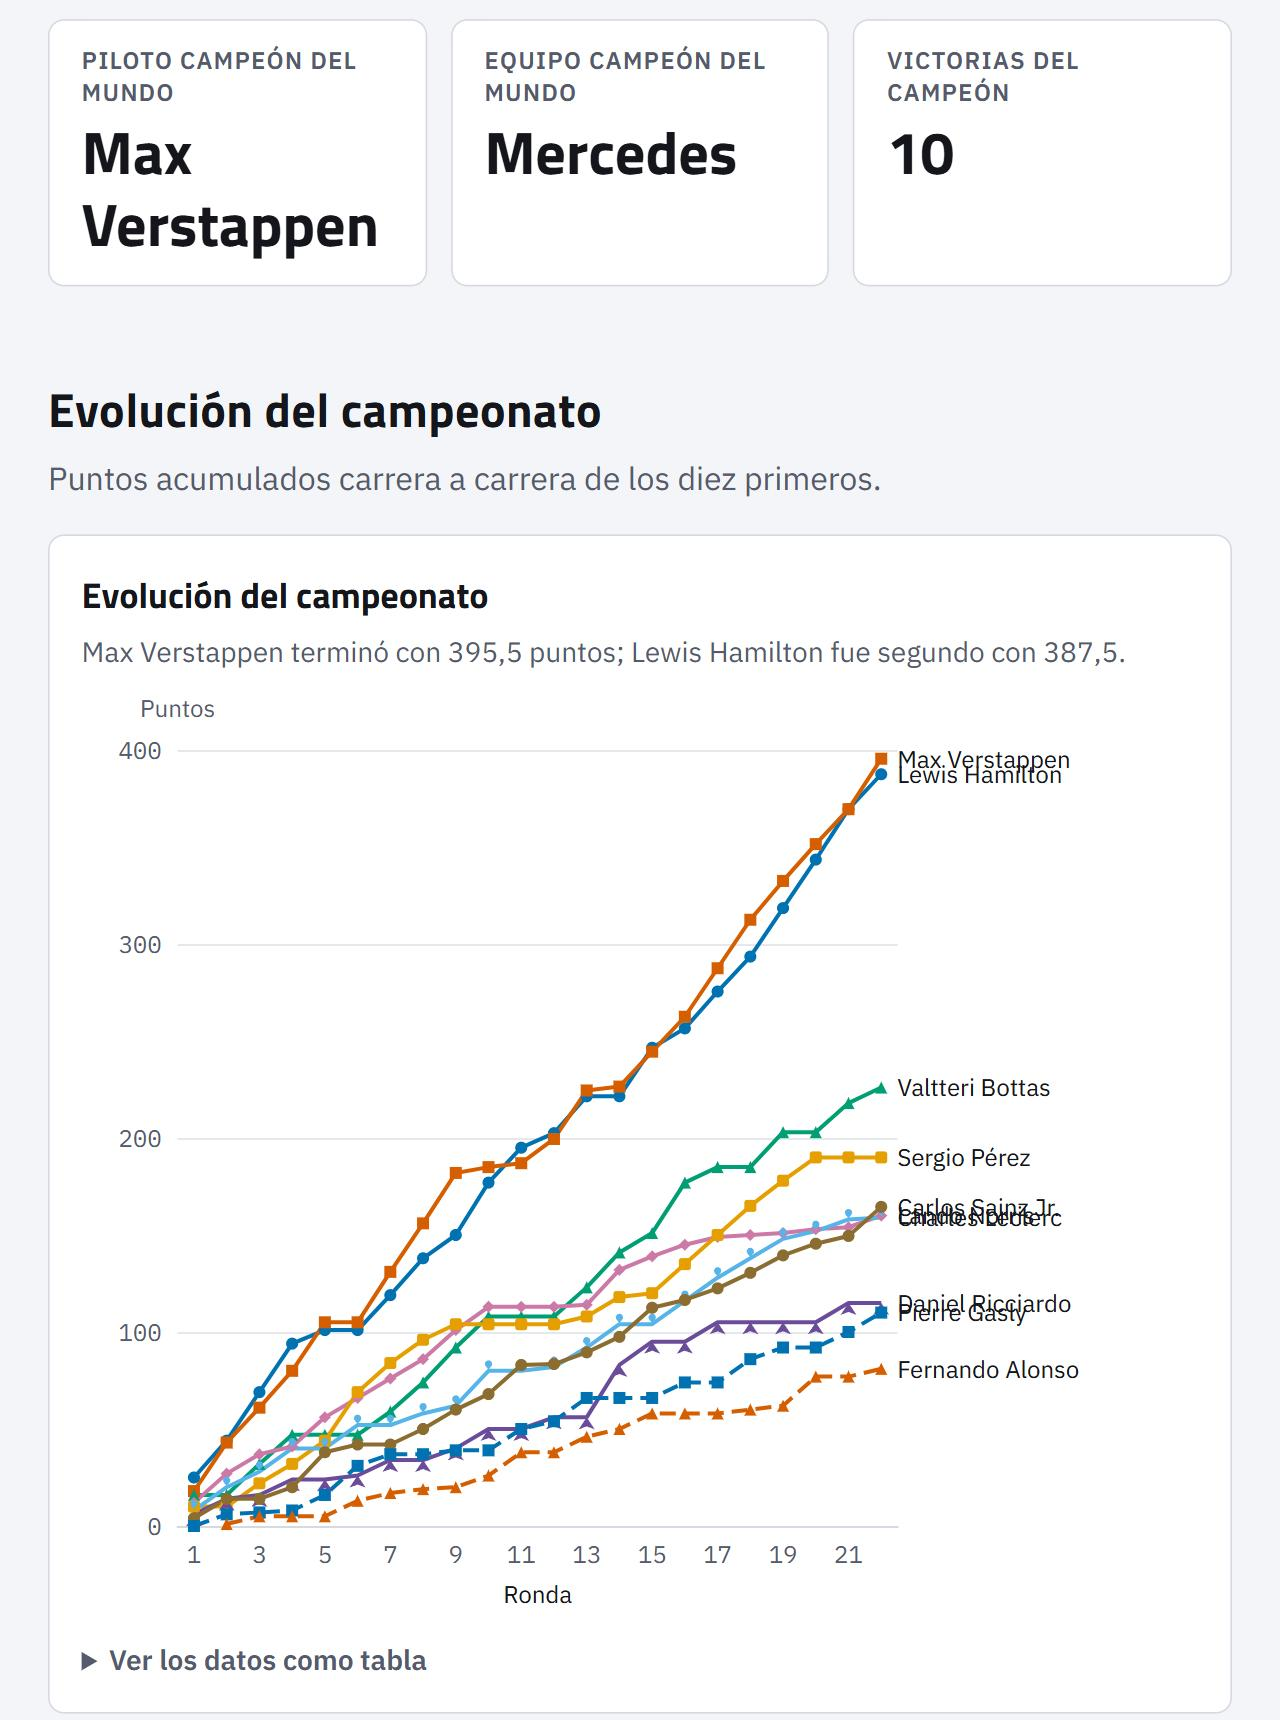
\includegraphics[width=\linewidth]{figuras/web_temporada2021_kpi_progresion.png}
\captionof{figure}{Temporada 2021: tarjetas que repiten la tabla y etiquetas solapadas al final
de la evolución del campeonato.}
\end{minipage}\hfill
\begin{minipage}[t]{0.48\linewidth}\centering
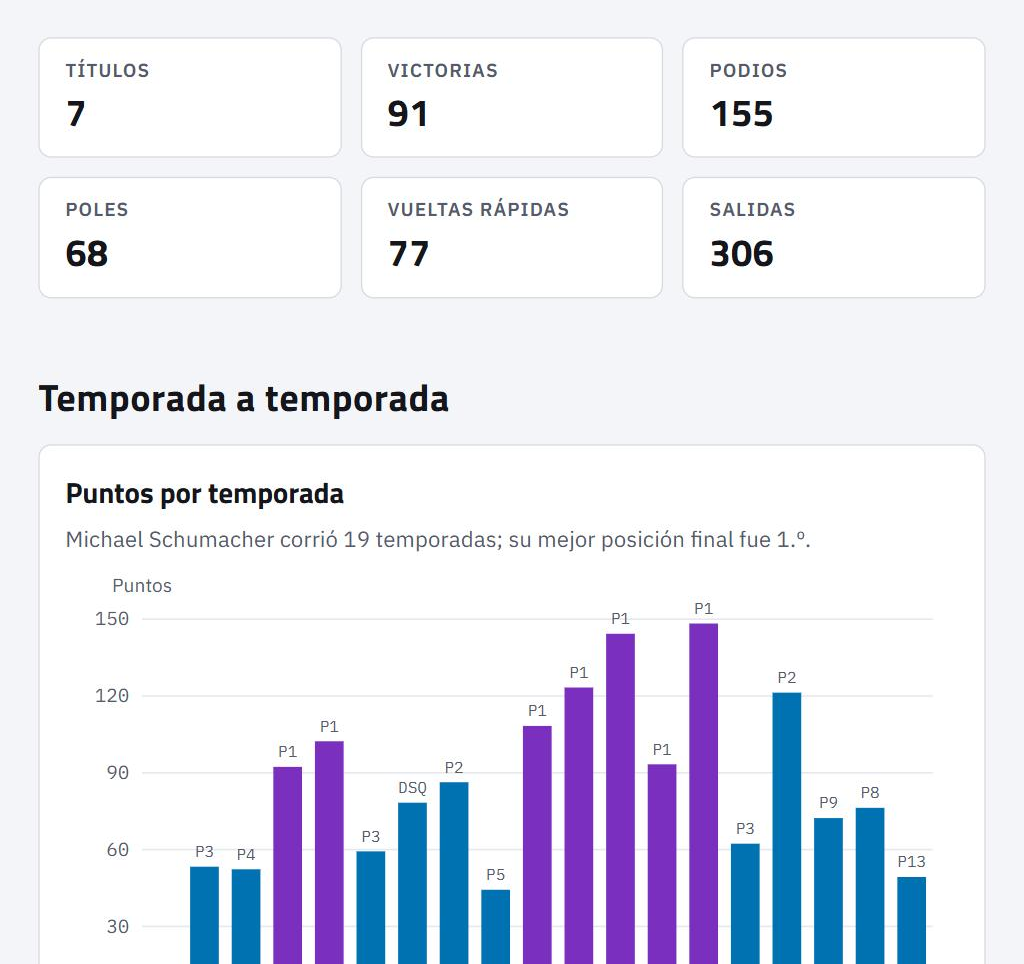
\includegraphics[width=\linewidth]{figuras/web_piloto_schumacher_kpi_puntos.png}
\captionof{figure}{Ficha de Michael Schumacher: los años sin carrera (2007–2009) desaparecen del
eje de temporadas.}
\end{minipage}
\end{figure}

\chapter{Evaluación de nuestros gráficos y propuestas nuevas}\label{cap:propios}
% Generado automáticamente desde notas/09_graficos_propios.md con md2tex.py; no editar a mano.
\begin{nota}
Estado: COMPLETA (29/09/2026).
\end{nota}

\section{Resumen}

\begin{itemize}
\item La web tiene \textbf{17 gráficos o mapas} en 16 entradas de inventario (13 ECharts, 1 violín SVG propio, 1 mapa mundial d3, 1 trazado SVG y 1 matriz-tabla), \textbf{15 tarjetas KPI} y unas \textbf{25 tablas}. Todos los gráficos van dentro de \code{Chart\allowbreak{}Figure}, con título, resumen en texto y la tabla de datos desplegable. La base de accesibilidad es buena y mejor que la de la mayoría de webs de F1.
\item Réplica del TFG: las páginas de las figuras 5.23-5.33 están todas (mapa, récords de pilotos y constructores, temporada, clasificación, vuelta a vuelta, neumáticos, tiempos, ritmo, boxes y detalle de piloto). Además hay extras: evolución del campeonato, telemetría con trazado, fichas de constructor y calidad de datos.
\item Problemas principales:
\begin{enumerate}
\item \textbf{Color sin identidad}: la paleta Okabe-Ito de 8 colores se repite en carreras de 20 pilotos. Los compañeros no comparten color de equipo y en el violín dos pilotos distintos salen con el mismo color sin otra diferencia.
\item \textbf{Solapamientos}: stints y matriz de neumáticos cuentan lo mismo. Hay tres gráficos y dos tablas de compañeros con la misma información. Las tarjetas de temporada repiten la tabla.
\item \textbf{Errores de lectura concretos}: la «referencia» de clasificación no es la pole. La duración de parada es el tiempo en el pit lane, no la parada. Las temporadas sin carrera desaparecen del eje. Ferrari tiene barras a 0 en 1950-57. Las etiquetas del final de la evolución del campeonato se solapan. «1,000 m» aparece con el formato inglés.
\item \textbf{Huecos de relato}: no hay página de circuito, ni «gap al líder», ni comparador libre de pilotos, ni fiabilidad o edades. Tampoco se ve cuándo se decidió el título.
\end{enumerate}
\item Propongo 26 visualizaciones nuevas (P1-P26, más la P1b), todas comprobadas contra \code{data/\allowbreak{}gold/\allowbreak{}f1.\allowbreak{}duckdb}, y una navegación con dos entradas nuevas: \textbf{Circuitos} y \textbf{Comparar}. Además, \textbf{Historia} agruparía Récords y las vistas por eras.
\end{itemize}

Fuentes: código de \code{web/\allowbreak{}src/\allowbreak{}app/\allowbreak{}[lang]/\allowbreak{}**} y \code{web/\allowbreak{}src/\allowbreak{}components/\allowbreak{}**} (sin modificar), la web desplegada (navegada el 29/09/2026 a 640 px y a 375 px de ancho), el TFG (texto de las figuras 5.23-5.33 extraído con \code{pdftotext}, porque el PDF no deja leerlo directamente) y \code{data/\allowbreak{}gold/\allowbreak{}f1.\allowbreak{}duckdb} en modo de solo lectura.

Capturas en \code{docs/\allowbreak{}informe\_\allowbreak{}situacion/\allowbreak{}figuras/\allowbreak{}}:

{\small\sloppy\setlength{\tabcolsep}{5pt}\renewcommand{\arraystretch}{1.15}
\begin{longtable}{@{}>{\raggedright\arraybackslash}p{0.393\dimexpr(\linewidth-20pt)\relax}>{\raggedright\arraybackslash}p{0.607\dimexpr(\linewidth-20pt)\relax}@{}}
\toprule
\textbf{Fichero} & \textbf{Contenido} \\
\midrule\endhead
\bottomrule\endlastfoot
\code{web\_\allowbreak{}lap\_\allowbreak{}chart\_\allowbreak{}bahrain2024.\allowbreak{}png} & Posiciones vuelta a vuelta, Bahrain 2024 \\
\code{web\_\allowbreak{}tiempos\_\allowbreak{}vuelta\_\allowbreak{}bahrain2024.\allowbreak{}png} & Tiempos por vuelta (20 pilotos) \\
\code{web\_\allowbreak{}violin\_\allowbreak{}bahrain2024.\allowbreak{}png} & Violines de ritmo \\
\code{web\_\allowbreak{}stints\_\allowbreak{}bahrain2024.\allowbreak{}png} & Estrategia de neumáticos \\
\code{web\_\allowbreak{}quali\_\allowbreak{}gap\_\allowbreak{}bahrain2024.\allowbreak{}png} & \% sobre el mejor tiempo (etiquetas solapadas) \\
\code{web\_\allowbreak{}telemetria\_\allowbreak{}bahrain2024.\allowbreak{}png} & Velocidad, acelerador y freno \\
\code{web\_\allowbreak{}temporada2021\_\allowbreak{}kpi\_\allowbreak{}progresion.\allowbreak{}png} & Tarjetas KPI y evolución del campeonato de 2021 (etiquetas solapadas) \\
\code{web\_\allowbreak{}piloto\_\allowbreak{}schumacher\_\allowbreak{}kpi\_\allowbreak{}puntos.\allowbreak{}png} & KPIs y puntos por temporada (los años 2007-2009 desaparecen del eje) \\
\code{web\_\allowbreak{}piloto\_\allowbreak{}schumacher\_\allowbreak{}companeros.\allowbreak{}png} & Gráficos de compañeros \\
\end{longtable}}

\medskip\noindent\textcolor{muted!40}{\rule{\linewidth}{0.3pt}}\medskip

\section{Método}

\begin{enumerate}
\item Lectura completa de las 17 páginas y de los 17 componentes visuales: tipos de marca, escalas, colores, datos de entrada y textos alternativos.
\item Navegación por la web desplegada: \code{/\allowbreak{}es}, \code{/\allowbreak{}es/\allowbreak{}seasons/\allowbreak{}2021}, \code{/\allowbreak{}es/\allowbreak{}races/\allowbreak{}1102} (Bahrain 2024) y sus pestañas, \code{/\allowbreak{}es/\allowbreak{}drivers/\allowbreak{}michael-\allowbreak{}schumacher}, \code{/\allowbreak{}es/\allowbreak{}constructors/\allowbreak{}ferrari} y \code{/\allowbreak{}es/\allowbreak{}records}. Se probó a 640 px y a 375 px de ancho.
\item Consultas de cobertura en DuckDB para saber qué gráficos se pueden dibujar y desde qué año (sección 5.0).
\end{enumerate}

\medskip\noindent\textcolor{muted!40}{\rule{\linewidth}{0.3pt}}\medskip

\section{Inventario completo}

Leyenda de accesibilidad:

\begin{itemize}
\item \textbf{F} = \code{Chart\allowbreak{}Figure}: título, resumen textual y tabla desplegable.
\item \textbf{img} = contenedor \code{role=\allowbreak{}"img"} con \code{aria-\allowbreak{}label}.
\item \textbf{T} = tabla semántica: \code{caption}, \code{scope} y región desplazable con el teclado.
\end{itemize}

\subsection{Gráficos y mapas}

{\scriptsize\sloppy\setlength{\tabcolsep}{4pt}\renewcommand{\arraystretch}{1.15}
\begin{longtable}{@{}>{\raggedright\arraybackslash}p{0.015\dimexpr(\linewidth-72pt)\relax}>{\raggedright\arraybackslash}p{0.094\dimexpr(\linewidth-72pt)\relax}>{\raggedright\arraybackslash}p{0.112\dimexpr(\linewidth-72pt)\relax}>{\raggedright\arraybackslash}p{0.152\dimexpr(\linewidth-72pt)\relax}>{\raggedright\arraybackslash}p{0.152\dimexpr(\linewidth-72pt)\relax}>{\raggedright\arraybackslash}p{0.139\dimexpr(\linewidth-72pt)\relax}>{\raggedright\arraybackslash}p{0.152\dimexpr(\linewidth-72pt)\relax}>{\raggedright\arraybackslash}p{0.139\dimexpr(\linewidth-72pt)\relax}>{\raggedright\arraybackslash}p{0.044\dimexpr(\linewidth-72pt)\relax}@{}}
\toprule
\textbf{\#} & \textbf{Ruta} & \textbf{Componente} & \textbf{Tipo} & \textbf{Datos (endpoint)} & \textbf{Pregunta que responde} & \textbf{Interacción} & \textbf{Accesibilidad} & \textbf{TFG} \\
\midrule\endhead
\bottomrule\endlastfoot
G1 & \code{/\allowbreak{}} (\#mapa) & \code{World\allowbreak{}Map} (d3-geo, SVG en servidor, sin JS) & Mapa de símbolos proporcionales (área ∝ √GP), proyección Equal Earth & \code{/\allowbreak{}circuits?season\_\allowbreak{}from\&season\_\allowbreak{}to}; en la vista por país, centroide ponderado por carreras & ¿Dónde se ha corrido la F1 y cuánto? & Por país o por circuito (enlaces); rango de temporadas (formulario GET); \code{<title>} en cada círculo & \code{<title>}/\code{<desc>}, figcaption y tabla por país o circuito & 5.23 \\
G2 & \code{/\allowbreak{}seasons/\allowbreak{}[year]} & \code{Progression\allowbreak{}Chart} & Líneas de puntos acumulados por ronda (top 10), con etiqueta al final & \code{/\allowbreak{}seasons/\allowbreak{}\{y\}/\allowbreak{}standings/\allowbreak{}progression?top=\allowbreak{}10} & ¿Cómo se fraguó el campeonato? & Tooltip por eje; resaltado de la serie al pasar & F, img, tabla piloto × ronda & Nuevo \\
G3 & \code{/\allowbreak{}races/\allowbreak{}[id]/\allowbreak{}qualifying} & \code{Bar\allowbreak{}Chart} vertical & Barras del \% sobre el mejor tiempo de la sesión; la mejor en morado & \code{/\allowbreak{}races/\allowbreak{}\{id\}/\allowbreak{}qualifying?session=\allowbreak{}} → \code{gap\_\allowbreak{}to\_\allowbreak{}pole\_\allowbreak{}pct} & ¿A cuánto quedó cada piloto o equipo del mejor tiempo? & Pilotos o constructores; Q o Q-sprint & F, img & 5.27 \\
G4 & \code{/\allowbreak{}races/\allowbreak{}[id]/\allowbreak{}lap-\allowbreak{}chart} & \code{Lap\allowbreak{}Chart} & Bump chart de posición por vuelta, con parrilla en la vuelta 0 y código del piloto al final & \code{/\allowbreak{}races/\allowbreak{}\{id\}/\allowbreak{}laps} + \code{/\allowbreak{}results} (parrilla) & ¿Cómo evolucionó el orden en carrera? & Resaltado al pasar; tooltip por punto & F, img, tabla salida/llegada/mejor/vueltas lideradas & 5.28 \\
G5 & \code{/\allowbreak{}races/\allowbreak{}[id]/\allowbreak{}tyres} & \code{Stint\allowbreak{}Chart} & Barras horizontales apiladas por stint; color Pirelli + letra & \code{/\allowbreak{}races/\allowbreak{}\{id\}/\allowbreak{}stints} & ¿Qué estrategia hizo cada uno? & Tooltip & F, img, leyenda con letra, tabla & 5.29 \\
G6 & \code{/\allowbreak{}races/\allowbreak{}[id]/\allowbreak{}tyres} (\#matriz) & \code{Compound\allowbreak{}Matrix} & Tabla-mapa de calor piloto × vuelta (compuesto; vuelta de entrada recuadrada) & \code{/\allowbreak{}races/\allowbreak{}\{id\}/\allowbreak{}laps} & ¿Qué neumático llevaba en cada vuelta y cuándo paró? & \code{title} por celda; desplazamiento horizontal & T con texto \code{sr-\allowbreak{}only} por celda & 5.29 (matriz) \\
G7 & \code{/\allowbreak{}races/\allowbreak{}[id]/\allowbreak{}pace} (\#tiempos) & \code{Lap\allowbreak{}Times\allowbreak{}Chart} & Líneas de tiempo por vuelta; 2 dataZoom (vueltas y tiempos) & \code{/\allowbreak{}races/\allowbreak{}\{id\}/\allowbreak{}laps} & ¿Cómo evolucionó el ritmo de cada piloto? & Casillas por piloto, Todos/Ninguno, ocultar vueltas neutralizadas, zoom & F, img, tabla vuelta × piloto & 5.30 \\
G8 & \code{/\allowbreak{}races/\allowbreak{}[id]/\allowbreak{}pace} (\#ritmo) & \code{Violin\allowbreak{}Chart} (SVG propio, KDE de Silverman) & Violín + caja P25-P75 + mediana por piloto, ordenado por mediana & Laps filtrados: sin vuelta 1, boxes, SC/VSC/roja ni vueltas >150 \% de la mediana; mín. 5 vueltas & ¿Quién tuvo mejor ritmo de verdad y lo mantuvo? & Casillas por piloto; \code{<title>} por violín & F, img, tabla mediana/mejor/P25-P75/nº & 5.31 \\
G9 & \code{/\allowbreak{}races/\allowbreak{}[id]/\allowbreak{}pitstops} & \code{Bar\allowbreak{}Chart} vertical & Barras del tiempo medio por equipo (paradas ≤ 60 s); la mejor en morado & \code{/\allowbreak{}races/\allowbreak{}\{id\}/\allowbreak{}pitstops} & ¿Qué equipo perdió menos tiempo en boxes? & Tooltip & F, img & 5.32 \\
G10 & \code{/\allowbreak{}races/\allowbreak{}[id]/\allowbreak{}telemetry} (desde 2024) & \code{Telemetry\allowbreak{}Chart} & 3 paneles con el eje X compartido: velocidad, acelerador y freno frente a la distancia & \code{/\allowbreak{}races/\allowbreak{}\{id\}/\allowbreak{}telemetry?drivers=\allowbreak{}a,\allowbreak{}b} (vuelta más rápida de clasificación) & ¿Dónde gana tiempo un piloto frente a otro? & Selector A/B (formulario GET); eje enlazado & F, img, tabla tiempo/v. máx./v. mín./\% a fondo & Nuevo \\
G11 & \code{/\allowbreak{}races/\allowbreak{}[id]/\allowbreak{}telemetry} & \code{Track\allowbreak{}Map} & Trazado x/y coloreado por velocidad (azul→naranja), solo del piloto A & Igual que G10 & ¿Cómo es el circuito y dónde es rápido o lento? & Ninguna & \code{<title>}/\code{<desc>}; leyenda con \code{aria-\allowbreak{}hidden} & Nuevo \\
G12 & \code{/\allowbreak{}drivers/\allowbreak{}[id]} & \code{Season\allowbreak{}Points\allowbreak{}Chart} & Barras de puntos por temporada; título en morado y posición final encima & \code{/\allowbreak{}drivers/\allowbreak{}\{id\}/\allowbreak{}seasons} & ¿Cómo fue su carrera deportiva año a año? & Tooltip & F, img, tabla temporada/equipo/pos./pts/V/P/poles & 5.33 (parcial) \\
G13 & \code{/\allowbreak{}drivers/\allowbreak{}[id]} & \code{Teammate\allowbreak{}Points\allowbreak{}Chart} & Barras agrupadas: puntos propios frente a los de sus compañeros (trama diagonal) & \code{/\allowbreak{}drivers/\allowbreak{}\{id\}/\allowbreak{}teammates} agregado por temporada & ¿Sumó más que sus compañeros? & Leyenda y tooltip & F, img, textura además del color & 5.33 \\
G14 & \code{/\allowbreak{}drivers/\allowbreak{}[id]} & \code{Teammate\allowbreak{}Share\allowbreak{}Chart} ×2 & Barras apiladas al 100 \%: \% por delante en clasificación y en carrera & Igual & ¿Batió a sus compañeros en clasificación y en carrera? & Leyenda y tooltip & F, img, textura & 5.33 \\
G15 & \code{/\allowbreak{}constructors/\allowbreak{}[id]} & \code{Season\allowbreak{}Points\allowbreak{}Chart} & Igual que G12 & \code{/\allowbreak{}constructors/\allowbreak{}\{id\}/\allowbreak{}seasons} & Evolución del equipo & Tooltip & F, img & Nuevo \\
G16 & \code{/\allowbreak{}records} & \code{Bar\allowbreak{}Chart} horizontal & Títulos por piloto o constructor en el rango de años & \code{/\allowbreak{}rankings/\allowbreak{}\{entity\}?order\_\allowbreak{}by=\allowbreak{}championships} & ¿Quién tiene más títulos en esa época? & Entidad y rango de años & F, img & 5.24-5.25 \\
\end{longtable}}

\subsection{Tarjetas KPI}

{\footnotesize\sloppy\setlength{\tabcolsep}{5pt}\renewcommand{\arraystretch}{1.15}
\begin{longtable}{@{}>{\raggedright\arraybackslash}p{0.156\dimexpr(\linewidth-40pt)\relax}>{\raggedright\arraybackslash}p{0.134\dimexpr(\linewidth-40pt)\relax}>{\raggedright\arraybackslash}p{0.435\dimexpr(\linewidth-40pt)\relax}>{\raggedright\arraybackslash}p{0.275\dimexpr(\linewidth-40pt)\relax}@{}}
\toprule
\textbf{Ruta} & \textbf{Componente} & \textbf{Contenido} & \textbf{TFG} \\
\midrule\endhead
\bottomrule\endlastfoot
\code{/\allowbreak{}seasons/\allowbreak{}[year]} & \code{Highlight} ×3 & Campeón (o líder), equipo campeón (o líder) y victorias del campeón & 5.26 (tarjetas de campeón y equipo) \\
\code{/\allowbreak{}drivers/\allowbreak{}[id]} & \code{Stat} ×6 & Títulos, victorias, podios, poles, vueltas rápidas y salidas & 5.33 (tarjetas superiores) \\
\code{/\allowbreak{}constructors/\allowbreak{}[id]} & \code{Stat} ×6 & Títulos, victorias, podios, poles, dobletes y carreras & Nuevo \\
\code{/\allowbreak{}quality} & Párrafo resumen & «N controles superados, M fallidos» & Nuevo \\
\end{longtable}}

\subsection{Tablas}

{\small\sloppy\setlength{\tabcolsep}{5pt}\renewcommand{\arraystretch}{1.15}
\begin{longtable}{@{}>{\raggedright\arraybackslash}p{0.181\dimexpr(\linewidth-30pt)\relax}>{\raggedright\arraybackslash}p{0.409\dimexpr(\linewidth-30pt)\relax}>{\raggedright\arraybackslash}p{0.409\dimexpr(\linewidth-30pt)\relax}@{}}
\toprule
\textbf{Ruta} & \textbf{Tabla} & \textbf{Observación} \\
\midrule\endhead
\bottomrule\endlastfoot
\code{/\allowbreak{}} & Top 10 de la última carrera; top 5 de pilotos y de constructores & Puerta de entrada; repite la página de temporada \\
\code{/\allowbreak{}seasons} & Tarjetas por década con los campeones & Es una lista de enlaces, sin datos \\
\code{/\allowbreak{}seasons/\allowbreak{}[year]} & Pilotos, constructores y calendario con ganador & Réplica de la figura 5.26 \\
\code{/\allowbreak{}races/\allowbreak{}[id]} & Resultado de carrera o sprint & Pills de vuelta rápida y dato corregido \\
\code{/\allowbreak{}races/\allowbreak{}[id]/\allowbreak{}qualifying} & Q1/Q2/Q3 con el mejor segmento en morado; \% & La columna de \% repite G3 \\
\code{/\allowbreak{}races/\allowbreak{}[id]/\allowbreak{}pitstops} & Lista de paradas; pasos por el pit lane que no son paradas & La segunda tabla es original y valiosa (SC, bandera roja, sanciones) \\
\code{/\allowbreak{}drivers}, \code{/\allowbreak{}constructors} & Top 50 por victorias o búsqueda & Sin orden por columnas (a diferencia de \code{/\allowbreak{}records}) \\
\code{/\allowbreak{}drivers/\allowbreak{}[id]} & Detalle de compañeros (temporada × compañero) & Más la tabla por temporada, repetida en los 3 gráficos \\
\code{/\allowbreak{}records} & Ranking ordenable (7 métricas) con rango de años & Réplica de las figuras 5.24-5.25 \\
\code{/\allowbreak{}quality} & Controles con umbral y controles informativos & Página original del proyecto \\
\end{longtable}}

\medskip\noindent\textcolor{muted!40}{\rule{\linewidth}{0.3pt}}\medskip

\section{Evaluación crítica}

\subsection{Problemas transversales}

\begin{enumerate}
\item \textbf{Color y paleta.}
\begin{itemize}
\item \code{LIGHT\_\allowbreak{}SERIES} tiene 8 colores. A partir del 9.º piloto el color se repite y cambia el trazo (discontinuo o punteado), lo que funciona en líneas finas.
\item En el \textbf{violín} (G8) no hay trazo que valga: Hülkenberg y Piastri salen del mismo marrón, y Stroll y Pérez del mismo naranja (captura \code{web\_\allowbreak{}violin\_\allowbreak{}bahrain2024.\allowbreak{}png}).
\item No se usa el color del equipo. El aficionado espera Ferrari en rojo y los dos compañeros con el mismo tono. \textbf{Dato que falta}: no hay colores de equipo en gold. \code{stg\_\allowbreak{}fastf1\_\allowbreak{}\_\allowbreak{}results.\allowbreak{}team\_\allowbreak{}color} existe, pero su vista apunta a un bronze que no está disponible (da error al consultarla), y además solo cubre 2018+. Propuesta: seed \code{constructor\_\allowbreak{}colors.\allowbreak{}csv} (id, temporada desde/hasta, hex claro y oscuro) y usar variantes claras y oscuras para distinguir a los compañeros, manteniendo el trazo o la forma.
\end{itemize}
\item \textbf{Ejes de temporadas como categorías.} \code{Season\allowbreak{}Points\allowbreak{}Chart} y \code{Teammate\allowbreak{}Points\allowbreak{}Chart} usan \code{type:\allowbreak{} "category"}, así que las temporadas sin carrera desaparecen. En Schumacher, 2006 va pegado a 2010 y parece que no hubo retirada. Debe ser un eje de valor (años) o marcar los huecos.
\item \textbf{Puntos entre eras.} Los gráficos de puntos por temporada (G12, G15) mezclan sistemas de puntuación: 9 puntos por victoria en 1950 frente a 25 hoy, y ahora más carreras. Los 148 puntos de Schumacher en 2004 parecen poco frente a los 575 de Verstappen en 2023. Hace falta una métrica normalizada (sección 5, P14).
\item \textbf{Base del eje en cero donde no aporta.}
\begin{itemize}
\item En la media de paradas (G9) las barras van de 24,1 a 27,2 s y el eje de 0 a 30: todas parecen iguales. En barras hay que empezar en 0, así que es mejor un gráfico de puntos o \emph{dot plot} con el eje ajustado, o mostrar la diferencia con el mejor.
\item En telemetría (G10) la velocidad empieza en 0 km/h y la mitad inferior del panel queda vacía.
\end{itemize}
\item \textbf{Formato numérico en ECharts.} Los ejes usan el formato por defecto de ECharts y aparece «1,000 m» en la página española. Los tooltips sí usan \code{to\allowbreak{}Locale\allowbreak{}String}. Falta un \code{axis\allowbreak{}Label.\allowbreak{}formatter} con \code{Intl.\allowbreak{}Number\allowbreak{}Format(\allowbreak{}locale)}.
\item \textbf{Etiquetas que se solapan.}
\begin{itemize}
\item \code{Progression\allowbreak{}Chart}: \code{label\allowbreak{}Layout.\allowbreak{}move\allowbreak{}Overlap} no se aplica a \code{end\allowbreak{}Label}. En 2021 «Max Verstappen» y «Lewis Hamilton» se pisan, y «Carlos Sainz Jr./Lando Norris/Charles Leclerc» no se leen.
\item Barras verticales de G3 con 20 pilotos: los valores «1,78 \%», «1,79 \%»… chocan entre sí y los nombres van girados 40°.
\end{itemize}
\item \textbf{Móvil (375 px).}
\begin{itemize}
\item El lap chart se comprime en \textasciitilde{}250 px de ancho y los intercambios en boxes forman una madeja ilegible.
\item Las pestañas de carrera y la navegación principal se desplazan en horizontal con una barra visible (se ve «Vuelta a vuelta» y la siguiente pestaña cortada).
\item El violín obliga a desplazarse en horizontal.
\item El mapa del inicio funciona bien porque es un SVG que se escala.
\end{itemize}
\item \textbf{Sin enlaces entre gráficos.} Ningún gráfico enlaza a la ficha del piloto o de la carrera (ECharts permite \code{on(\allowbreak{}'click')}) ni recuerda la selección de pilotos entre pestañas. Las casillas de G7 y G8 son independientes: el aficionado marca 3 pilotos en tiempos y tiene que volver a marcarlos en el violín.
\item \textbf{Accesibilidad.} Lo correcto: figura, resumen, tabla, letras en compuestos, texturas en compañeros y \code{prefers-\allowbreak{}reduced-\allowbreak{}motion}. Mejorable:
\begin{itemize}
\item \code{aria.\allowbreak{}enabled:\allowbreak{} false} es deliberado (la tabla sustituye al gráfico), pero el tooltip no es accesible con el teclado. No hay forma de «recorrer» la serie.
\item El texto del violín es de 10 px dentro de un \code{view\allowbreak{}Box} que se escala hacia abajo: en la práctica queda por debajo de 8 px (captura).
\item El resumen de G16 dice «Lewis Hamilton suma más títulos: 7» cuando empata con Schumacher. Los resúmenes deberían detectar empates.
\end{itemize}
\item \textbf{Rendimiento y carga.} Cada pestaña de carrera vuelve a pedir \code{/\allowbreak{}laps} (unas 1 200 filas) y \code{/\allowbreak{}results}. Hay \code{cache} por petición, pero no entre pestañas. Es aceptable, aunque con Render free la primera visita tarda.
\end{enumerate}

\subsection{Evaluación de cada elemento}

{\footnotesize\sloppy\setlength{\tabcolsep}{5pt}\renewcommand{\arraystretch}{1.15}
\begin{longtable}{@{}>{\raggedright\arraybackslash}p{0.155\dimexpr(\linewidth-50pt)\relax}>{\raggedright\arraybackslash}p{0.159\dimexpr(\linewidth-50pt)\relax}>{\raggedright\arraybackslash}p{0.229\dimexpr(\linewidth-50pt)\relax}>{\raggedright\arraybackslash}p{0.229\dimexpr(\linewidth-50pt)\relax}>{\raggedright\arraybackslash}p{0.229\dimexpr(\linewidth-50pt)\relax}@{}}
\toprule
\textbf{\#} & \textbf{Valoración} & \textbf{Puntos fuertes} & \textbf{Problemas concretos} & \textbf{Recomendación} \\
\midrule\endhead
\bottomrule\endlastfoot
G1 Mapa & \textbf{Útil} & Sin JS; rango de años; 2 vistas; tabla & Europa es una mancha de círculos que se solapan; el centroide por país sitúa a EE. UU. en medio del país y no en sus circuitos; no muestra el tiempo & Añadir un zoom a Europa (inserto) o una vista de «calendario por país × década» (P9); color por última temporada (vigente o histórico) \\
G2 Evolución campeonato & \textbf{Muy útil} & Cuenta la temporada; tabla completa & Etiquetas solapadas; 10 líneas con colores repetidos; los puntos absolutos esconden la diferencia en la lucha por el título & Añadir el modo «diferencia con el líder» (P1), resaltar por defecto los 2-3 aspirantes, marcar la ronda en que se decidió (\code{drivers\_\allowbreak{}championship\_\allowbreak{}decider}) \\
G3 \% sobre el mejor tiempo & \textbf{Útil, con un fallo de relato} & Métrica fiel al TFG; modo por constructores & (1) La referencia es el mejor tiempo de cualquier segmento: en Bahrain 2024 la «referencia» es Leclerc (Q2, 1:29.165) y Verstappen, que hizo la pole, aparece a +0,016 \%; el resumen dice «Leclerc marcó la referencia», lo que confunde. (2) Mezcla segmentos con distinta evolución de pista: Stroll (eliminado en Q2) queda por delante de Tsunoda porque su Q1 fue mejor. (3) Barras verticales con 20 nombres girados y etiquetas solapadas & Barras horizontales (como G16); nombrar la métrica «mejor vuelta de la sesión»; opción «por segmento» (Q1/Q2/Q3 por separado); marcar la línea de corte de Q1 y Q2 \\
G4 Lap chart & \textbf{Muy útil} & Etiqueta directa; parrilla en la vuelta 0; tabla con vueltas lideradas & Madeja en las ventanas de paradas (vueltas 10-17 y 30-38 en Bahrain); con 20 pilotos no se sigue a nadie salvo al que se resalta; no marca SC, abandonos ni paradas; datos desde 1950, pero en los años 50 solo el 56 \% de las posiciones por vuelta tienen dato, así que las líneas salen rotas & Resaltar por defecto el top 3 y atenuar al resto; marcar las paradas con puntos y el SC/VSC con bandas; ofrecer al lado un «race trace» (P1b), que responde mejor a la pregunta «quién ganó por estrategia» \\
G5 Stints & \textbf{Muy útil} & Claro y fiel a la convención de la TV; letra en cada tramo; el duro con contorno & Eje hasta 60 cuando la carrera tiene 57 vueltas; no distingue neumático nuevo o usado (el 20 \% de los stints de 2024 salen con más de 1 vuelta de uso, según \code{tyre\_\allowbreak{}age\_\allowbreak{}laps}); el primer stint de 1 vuelta (Hülkenberg) sale sin letra & \code{max =\allowbreak{} vueltas}; trama o transparencia para los usados; tooltip con la edad inicial \\
G6 Matriz & \textbf{Poco útil} (repetida) & Réplica fiel del TFG; accesible & Da la misma información que G5 en 20 × 57 celdas; obliga a desplazarse en horizontal; el recuadro de la vuelta de entrada no añade nada a los cortes de G5 & Fusionarla con G5 como su «tabla de datos», o reutilizar la forma de la matriz para algo nuevo: mapa de calor del \textbf{tiempo por vuelta respecto a la mediana} o de la \textbf{posición} (P3) \\
G7 Tiempos por vuelta & \textbf{Útil} para 2-4 pilotos, \textbf{poco útil} con 20 & Zoom doble (fiel al TFG); ocultar neutralizadas activado si hace falta; tabla completa & Con 20 líneas y 8 colores es ilegible (captura); las vueltas de boxes cortan las líneas; el eje de tiempos no es invertido (en F1 «más rápido» se suele dibujar arriba o se dibuja el delta) & Por defecto, solo el top 3 o los dos del mismo equipo; añadir la vista «delta con un piloto de referencia»; opción de corregir el combustible (P2) \\
G8 Violín & \textbf{Muy útil} & Filtro de vueltas cuidado (incluye la heurística del 150 \%); orden por mediana; tabla & Colores repetidos sin otra diferencia; texto diminuto; ticks con valores extraños (1:41.470, 1:39.698…) en lugar de valores redondos; la cola de VER hasta 1:32.6 (vuelta rápida con blandos nuevos) alarga mucho la escala & Ticks redondos (cada 0,5 s o 1 s); color de equipo; nombres horizontales más grandes; opción de dividir el violín por compuesto (mitad izquierda y derecha, \emph{split violin}) (P4) \\
G9 Media de paradas & \textbf{Poco útil tal como está} & Réplica del TFG; umbral de 60 s & La «duración» es el \textbf{tiempo en el pit lane} (mediana 2020s: 23,9 s), no la parada estática (unos 2-3 s), y el título no lo aclara; el eje en 0 aplana las diferencias; la media esconde las paradas malas & Renombrarlo a «Tiempo en el pit lane»; usar \emph{strip plot} (una marca por parada) con la mediana; dato que falta: la parada estática (DHL Fastest Pit Stop o documentos de la FIA) \\
G10 Telemetría & \textbf{Útil} (con un fallo de relato) & Tres paneles enlazados; selector A/B sin JS & Es la \textbf{vuelta rápida de clasificación} dentro de una pestaña de carrera y el título no lo dice; no hay \textbf{delta de tiempo acumulado} (lo más informativo en una comparación de telemetría); \code{rpm}, \code{gear} y \code{drs} están al 100 \% en gold pero no se usan; velocidad desde 0; el eje Y del freno sin sentido; «1,000 m» & Titular «Vuelta rápida de clasificación»; añadir el panel de delta (se integra con distancia y velocidad) y el de marchas; ajustar el eje de velocidad; ver P6 y P7 \\
G11 Trazado & \textbf{Útil} (atractivo) & Proporciones reales; escala continua & Solo el piloto A; no enseña la comparación que se acaba de elegir; la escala azul→naranja no marca dónde está la curva lenta & «Dominio por minisectores» A frente a B (P6) y el número de curva o la marcha en el trazado \\
G12 Puntos por temporada (piloto) & \textbf{Útil} & Título en morado; posición encima & Eje de categorías (se pierden los huecos); puntos no comparables entre eras; la barra no dice con qué equipo corrió & Eje temporal; alternar puntos, posición final y \% de puntos posibles; color por equipo (P13) \\
G13 Puntos frente a compañeros & \textbf{Poco útil} (repetido) & Textura accesible & Repite lo que ya dicen G14 y la tabla; al sumar a varios compañeros en una temporada (1994: Verstappen + Lehto + Herbert) se mezclan duelos distintos & Fusionar con G14 en un solo gráfico de barras divergentes por temporada y compañero (P12) \\
G14 H2H clasificación y carrera (×2) & \textbf{Útil} & Porcentajes claros & Dos gráficos casi iguales uno al lado del otro; el apilado al 100 \% gasta la mitad de la tinta en el «complemento» & Un único gráfico divergente: clasificación a la izquierda y carrera a la derecha, o 2 puntos por temporada \\
G15 Puntos por temporada (constructor) & \textbf{Poco útil} en equipos históricos & — & Ferrari 1950-57: el campeonato de constructores empezó en 1958, así que salen barras a 0 (el \code{points ?? 0} del código) con 3-7 victorias por temporada; puntos no comparables & Para antes de 1958, mostrar victorias o puntos de sus pilotos o un marcador «sin campeonato»; métrica normalizada \\
G16 Títulos & \textbf{Útil} & Horizontal, legible & Repite la columna «Títulos» de la tabla ordenable de al lado; el resumen no detecta el empate & Sustituirlo por algo que la tabla no dé: «títulos a lo largo del tiempo» (línea de tiempo por piloto, P16) \\
KPI temporada & \textbf{Poco útil} & Réplica fiel del TFG & El campeón sale 3 veces (tarjeta, pill en la tabla y resumen de G2); «victorias del campeón» es un dato pobre & Sustituirlas por KPIs de relato: margen del título, ronda de la decisión, nº de ganadores distintos, dominio del equipo (\% de victorias) \\
KPI piloto y constructor & \textbf{Útil} & Resumen rápido & Sin contexto (¿91 victorias es mucho?) & Añadir el percentil o el puesto histórico («2.º de todos los tiempos») o el porcentaje (\code{win\_\allowbreak{}rate\_\allowbreak{}pct} y \code{podium\_\allowbreak{}rate\_\allowbreak{}pct} existen en \code{agg\_\allowbreak{}driver\_\allowbreak{}career}) \\
Tabla de pasos por el pit lane & \textbf{Muy útil} y original & Distingue parada, SC, bandera roja y abandono & Poco visible, al final de la pestaña & Integrarla como marcas en G4 y G5 \\
\code{/\allowbreak{}quality} & \textbf{Útil} para el TFG y la transparencia & — & Solo tablas & Opcional: gráfico de barras de \% de coincidencia con la línea del umbral \\
\end{longtable}}

\subsection{Repeticiones y solapamientos (qué fusionar o eliminar)}

{\small\sloppy\setlength{\tabcolsep}{5pt}\renewcommand{\arraystretch}{1.15}
\begin{longtable}{@{}>{\raggedright\arraybackslash}p{0.192\dimexpr(\linewidth-30pt)\relax}>{\raggedright\arraybackslash}p{0.404\dimexpr(\linewidth-30pt)\relax}>{\raggedright\arraybackslash}p{0.404\dimexpr(\linewidth-30pt)\relax}@{}}
\toprule
\textbf{Solapamiento} & \textbf{Elementos} & \textbf{Propuesta} \\
\midrule\endhead
\bottomrule\endlastfoot
\textbf{Estrategia de neumáticos} & G5 stints + G6 matriz + tabla de stints & Dejar G5. La matriz pasa a ser su tabla alternativa o se reutiliza como mapa de calor del ritmo (P3) \\
\textbf{Ritmo de carrera} & G4 posiciones + G7 tiempos + G8 violín & Cada uno responde a algo distinto, pero G7 con 20 pilotos no responde a nada. Propuesta: pestaña «Carrera» con G4 y el race trace (P1b); pestaña «Ritmo» con el violín y G7 limitado a 2-4 pilotos o en modo delta \\
\textbf{Compañeros de equipo} & G13 + G14 ×2 + tabla por temporada (repetida 3 veces como tabla de cada figura) + tabla de detalle & Un único gráfico divergente (P12) + una tabla de detalle \\
\textbf{Campeón de la temporada} & 3 tarjetas + pill de la tabla + resumen de G2 + tarjeta en \code{/\allowbreak{}seasons} & Tarjetas de relato (ver KPI temporada) \\
\textbf{\% en clasificación} & G3 + columna \% de la tabla de clasificación & Aceptable (la tabla es la referencia), pero G3 debería aportar algo más (segmentos, cortes) \\
\textbf{Títulos} & G16 + columna «Títulos» del ranking & Sustituir G16 (P16) \\
\textbf{Inicio frente a temporada} & Top 5 de pilotos y constructores del inicio = tabla de la temporada actual & Aceptable como portada; mejor un «mini G2» (la lucha por el título en una línea) \\
\textbf{Puntos por temporada} & G12 (piloto) y G15 (constructor) con el mismo componente & Correcto (reutilización); arreglar los ejes y la normalización \\
\textbf{Salida y llegada} & Tabla de G4 (salida, llegada) y tabla de resultado (parrilla, posición) & Aceptable \\
\end{longtable}}

\subsection{Huecos de relato (preguntas típicas de un aficionado sin respuesta)}

\begin{enumerate}
\item \textbf{«¿Por cuánto ganó y cuándo se decidió la carrera?»} No hay diferencias en el tiempo. \code{gap\_\allowbreak{}to\_\allowbreak{}leader\_\allowbreak{}ms} está al 84-100 \% desde 2022, y el tiempo acumulado (Σ \code{lap\_\allowbreak{}time\_\allowbreak{}ms}) lo reconstruye exactamente desde 1996: en Bahrain 2024, vuelta 30, el cálculo coincide con la fuente al centésimo.
\item \textbf{«¿Hubo adelantamientos? ¿Fue una carrera entretenida?»} No hay índice de cambios de posición ni de cambios de líder (calculable: media de cambios de líder por carrera de 4,0 en los 50, 1,8 en los 70 y 2,7 en los 2020).
\item \textbf{«¿Qué pasa en este circuito?»} No hay \textbf{página de circuito}, aunque \code{dim\_\allowbreak{}race} tiene 78 circuitos con lat/lon, tipo, sentido, longitud y curvas. No se ven ganadores por circuito, conversión de la pole en victoria (Yas Marina 70,6 \%, Catalunya 69,4 \%…), probabilidad de SC ni récord de vuelta.
\item \textbf{«¿Quién es mejor: X o Y?»} No hay un comparador libre de pilotos. Solo se compara con los compañeros o, en telemetría, en una sesión.
\item \textbf{«¿Cuándo se decidió el título y quién podía ganarlo todavía?»} Hay 76 carreras marcadas como \code{drivers\_\allowbreak{}championship\_\allowbreak{}decider}, pero no se usan. Tampoco se calcula la eliminación matemática.
\item \textbf{Fiabilidad y abandonos por época.} \code{reason\_\allowbreak{}retired} tiene datos de todas las décadas. Los clasificados pasan del 41 \% en los 80 al 87 \% en los 2020, y la parte mecánica de los abandonos baja del 86 \% al 55 \%.
\item \textbf{Edades y carreras deportivas.} Ganador más joven (Verstappen, 18,6 años) y edad media de la parrilla (35,1 en los 50 frente a 28,4 en los 2020). \code{date\_\allowbreak{}of\_\allowbreak{}birth} está al 100 \%.
\item \textbf{Nacionalidades y «victorias en casa».} Hay 95 victorias en casa de 1 167.
\item \textbf{Equipos y motores.} No se ve el motor por equipo y temporada, aunque \code{engine\_\allowbreak{}manufacturer\_\allowbreak{}id} está en los resultados. Tampoco hay una línea de tiempo de las alineaciones.
\item \textbf{Sprint.} Hay resultado de sprint, pero no vueltas (ver nota 03).
\item \textbf{Datos que no tenemos.} Meteorología, mensajes de dirección de carrera (solo hay banderas por vuelta), parada estática y adelantamientos oficiales.
\end{enumerate}

\medskip\noindent\textcolor{muted!40}{\rule{\linewidth}{0.3pt}}\medskip

\section{Propuestas nuevas}

\subsection{Qué se puede dibujar y desde cuándo (comprobado en \code{data/\allowbreak{}gold/\allowbreak{}f1.\allowbreak{}duckdb})}

{\small\sloppy\setlength{\tabcolsep}{5pt}\renewcommand{\arraystretch}{1.15}
\begin{longtable}{@{}>{\raggedright\arraybackslash}p{0.253\dimexpr(\linewidth-30pt)\relax}>{\raggedright\arraybackslash}p{0.373\dimexpr(\linewidth-30pt)\relax}>{\raggedright\arraybackslash}p{0.373\dimexpr(\linewidth-30pt)\relax}@{}}
\toprule
\textbf{Dato} & \textbf{Tabla y columna} & \textbf{Cobertura} \\
\midrule\endhead
\bottomrule\endlastfoot
Posición por vuelta & \code{fact\_\allowbreak{}laptimes.\allowbreak{}position} & Las 1 164 carreras disputadas desde 1950 (56 \% de las filas con dato en los 50, 95 \% en los 60, 100 \% desde los 70) \\
Tiempo por vuelta & \code{fact\_\allowbreak{}laptimes.\allowbreak{}lap\_\allowbreak{}time\_\allowbreak{}ms} & 0 \% antes de 1990, 96,5 \% en los 90, \textasciitilde{}100 \% desde 2000 (desde 1996 en la práctica) \\
Gap al líder & \code{gap\_\allowbreak{}to\_\allowbreak{}leader\_\allowbreak{}ms} & 60-87 \% por temporada desde 1996, 100 \% en 2025-26; \textbf{reconstruible} exactamente con Σ \code{lap\_\allowbreak{}time\_\allowbreak{}ms} (comprobado en Bahrain 2024, vuelta 30: Pérez +15,68 s, Sainz +18,20 s en ambos cálculos) \\
Compuesto y edad del neumático & \code{tyre\_\allowbreak{}compound}, \code{tyre\_\allowbreak{}age\_\allowbreak{}laps} & Desde 2011 (100 \%); compuesto Pirelli C1-C5 desde 2019 \\
Sectores y speed trap & \code{sector\_\allowbreak{}*\_\allowbreak{}ms}, \code{speed\_\allowbreak{}trap\_\allowbreak{}kmh} & Desde 2018 (98 \%) \\
Banderas por vuelta & \code{is\_\allowbreak{}safety\_\allowbreak{}car}, \code{is\_\allowbreak{}yellow\_\allowbreak{}flag}, \code{is\_\allowbreak{}virtual\_\allowbreak{}safety\_\allowbreak{}car}, \code{is\_\allowbreak{}red\_\allowbreak{}flag} & SC desde los 90 (1 922 vueltas), VSC desde 2015, bandera roja desde 2000 \\
Paradas & \code{fact\_\allowbreak{}pit\_\allowbreak{}stops.\allowbreak{}time\_\allowbreak{}ms} & Desde 1994 (612 carreras); es el tiempo \textbf{en el pit lane} (mediana de 30,0 s en los 90 y 23,9 s en los 2020) \\
Pasos por el pit lane & \code{fact\_\allowbreak{}pit\_\allowbreak{}lane\_\allowbreak{}passes.\allowbreak{}pass\_\allowbreak{}type} & pit\_stop 22 485, unclassified 1 118, retirement 351, penalty\_or\_other 141, safety\_car 114, red\_flag 62 \\
Telemetría de clasificación & \code{fact\_\allowbreak{}quali\_\allowbreak{}telemetry} & 2024-2026 (63 carreras); \textasciitilde{}450 puntos por vuelta; velocidad, rpm, marcha, acelerador, freno, DRS y x/y al 100 \% \\
Clasificación del campeonato por ronda & \code{fact\_\allowbreak{}driver\_\allowbreak{}standing}, \code{fact\_\allowbreak{}constructor\_\allowbreak{}standing} & Todas las rondas desde 1950 (1950: 108/108 filas con posición) \\
Resultado & \code{fact\_\allowbreak{}race\_\allowbreak{}result} & Parrilla \textasciitilde{}90 \%; \code{reason\_\allowbreak{}retired} con 198 valores distintos; \code{positions\_\allowbreak{}gained}; \code{is\_\allowbreak{}grand\_\allowbreak{}slam} (71); piloto del día (2016+, 228) \\
Q1/Q2/Q3 & \code{fact\_\allowbreak{}qualifying\_\allowbreak{}result} & Desde 2006 (40 \% de los 2000, \textasciitilde{}99 \% desde 2010); mejor tiempo desde 1950 (96 \%) \\
Carrera & \code{dim\_\allowbreak{}race} & 78 circuitos con lat/lon, tipo (ROAD/RACE/STREET), sentido, longitud, curvas; \code{drivers\_\allowbreak{}championship\_\allowbreak{}decider} (76 carreras) \\
Piloto & \code{dim\_\allowbreak{}driver} & \code{date\_\allowbreak{}of\_\allowbreak{}birth} 100 \% (917 pilotos), nacionalidad alpha2 \\
Compañeros & \code{agg\_\allowbreak{}teammate\_\allowbreak{}h2h} & 13 530 filas; grafo de 4 componentes conexas, con 810 pilotos en la mayor \\
\end{longtable}}

\textbf{Datos que faltan} para algunas propuestas:

\begin{itemize}
\item \textbf{Colores de equipo por temporada}: hace falta un seed. La vista \code{stg\_\allowbreak{}fastf1\_\allowbreak{}\_\allowbreak{}results.\allowbreak{}team\_\allowbreak{}color} apunta a un bronze que no está disponible y solo cubriría 2018+.
\item \textbf{Clasificación de \code{reason\_\allowbreak{}retired}} en mecánico, accidente u otro: seed de unas 200 filas.
\item \textbf{Parada estática} (solo tenemos el tiempo en el pit lane).
\item \textbf{Meteorología}.
\item \textbf{Mensajes de dirección de carrera} (solo hay banderas por vuelta).
\item \textbf{Vueltas de sprint} (ver nota 03).
\item \textbf{Adelantamientos oficiales}: los cambios de posición son un proxy.
\end{itemize}

Esfuerzo: \textbf{S} = menos de 1 día (reutiliza un endpoint o componente existente); \textbf{M} = 1-3 días (endpoint o modelo dbt nuevo); \textbf{L} = más de 3 días.

\subsection{Carrera (pestañas de \code{/\allowbreak{}races/\allowbreak{}[id]})}

\textbf{P1b. Race trace: diferencia con el líder vuelta a vuelta.} \emph{Esfuerzo S-M.}

\begin{itemize}
\item Pregunta: ¿por cuánto iba ganando, cuándo se abrió o cerró la carrera y qué hizo el SC con las diferencias?
\item Boceto:
\begin{itemize}
\item Eje X: vuelta. Eje Y: segundos detrás del líder, invertido, con el líder en 0 arriba.
\item Una línea por piloto; las vueltas bajo SC/VSC como bandas grises de fondo y las paradas como puntos huecos.
\item Etiqueta directa al final. Por defecto se resalta el top 5 y el resto va en gris al 25 \%.
\item Variante: «delta con un piloto elegido» (la referencia horizontal es ese piloto).
\end{itemize}
\item Datos: \code{fact\_\allowbreak{}laptimes} (Σ \code{lap\_\allowbreak{}time\_\allowbreak{}ms} por piloto y vuelta; en cada vuelta, referencia = mínimo acumulado), \code{is\_\allowbreak{}safety\_\allowbreak{}car}/\code{is\_\allowbreak{}virtual\_\allowbreak{}safety\_\allowbreak{}car}, \code{is\_\allowbreak{}pit\_\allowbreak{}in\_\allowbreak{}lap}. Desde 1996.
\item Dónde: pestaña «Vuelta a vuelta», junto a G4, con un conmutador «posiciones | diferencias».
\item Accesibilidad: resumen generado («X abrió N s en M vueltas; el SC de la vuelta K dejó la ventaja en 1 s») y tabla vuelta × piloto.
\end{itemize}

\textbf{P2. Degradación por stint.} \emph{Esfuerzo M.}

\begin{itemize}
\item Pregunta: ¿quién cuidó mejor los neumáticos? ¿Cuánto perdía por vuelta cada compuesto?
\item Boceto:
\begin{itemize}
\item (a) \emph{Dot plot}: una fila por piloto; cada stint es un punto en X = pendiente en ms/vuelta, con color y letra del compuesto.
\item (b) Al pulsar un piloto, dispersión de tiempo corregido frente a la edad del neumático, con su recta de regresión por stint.
\item Corrección de combustible: restar la tendencia común de la carrera (mediana por vuelta de todos los pilotos) o un coeficiente fijo documentado como estimación.
\end{itemize}
\item Datos: \code{regr\_\allowbreak{}slope(\allowbreak{}lap\_\allowbreak{}time\_\allowbreak{}ms,\allowbreak{} tyre\_\allowbreak{}age\_\allowbreak{}laps)} por (piloto, stint) sobre vueltas limpias (sin vuelta 1, boxes ni SC/VSC; mínimo 8 vueltas). Probado en Bahrain 2024: pendientes de 6 a 123 ms/vuelta (Leclerc: 84 ms/vuelta con blando y 6 con el primer duro). La dispersión muestra que la corrección de combustible es imprescindible antes de publicarlo. Desde 2011.
\item Dónde: pestaña «Neumáticos» o «Estrategia», \textbf{en lugar de la matriz G6}.
\item Accesibilidad: tabla piloto/stint/compuesto/vueltas/pendiente; resumen «el que menos degradó con duro fue X».
\end{itemize}

\textbf{P3. Mapa de calor del ritmo (reutiliza la forma de la matriz).} \emph{Esfuerzo S.}

\begin{itemize}
\item Pregunta: ¿en qué fase de la carrera fue rápido cada piloto?
\item Boceto:
\begin{itemize}
\item Filas = pilotos (orden de llegada); columnas = vueltas.
\item Color divergente = diferencia con la mediana de la vuelta, con los rápidos en azul y los lentos en naranja (apto para daltonismo).
\item Vueltas neutralizadas rayadas, paradas recuadradas y la letra del compuesto opcional.
\end{itemize}
\item Datos: los mismos \code{laps} que usa hoy G6.
\item Dónde: sustituye a G6.
\item Accesibilidad: sigue siendo una \code{<table>} con el valor en texto \code{sr-\allowbreak{}only}, igual que la matriz actual.
\end{itemize}

\textbf{P4. Violín partido por compuesto.} \emph{Esfuerzo S.}

\begin{itemize}
\item Pregunta: ¿el ritmo de X era mejor con medio o con duro?
\item Boceto: mitad izquierda del violín con el compuesto 1 y mitad derecha con el compuesto 2, en colores Pirelli con contorno; ticks redondos.
\item Datos: los de G8 más \code{tyre\_\allowbreak{}compound}.
\item Dónde: opción de G8.
\item Accesibilidad: la tabla gana una columna por compuesto.
\end{itemize}

\textbf{P5. Detector de undercut y overcut.} \emph{Esfuerzo M.} No lo he visto como gráfico automático en otras webs de aficionados.

\begin{itemize}
\item Pregunta: ¿quién ganó o perdió posiciones por la estrategia de paradas?
\item Boceto:
\begin{itemize}
\item Lista de «duelos de estrategia»; cada duelo es un mini \emph{slope chart} con dos puntos (antes y después) y dos líneas (A y B).
\item Etiqueta: «Norris paró 2 vueltas antes que Leclerc → undercut logrado (+1 posición)».
\item Verde u óxido según el resultado, con icono \si{}/\no{} para no depender del color.
\end{itemize}
\item Datos:
\begin{itemize}
\item Heurística: A y B van consecutivos en pista la vuelta anterior a la parada de A; B para entre 1 y 3 vueltas después; se comparan las posiciones en la vuelta \code{lb+2}.
\item Resultado en 2024: \textbf{204 intentos, 49 undercuts logrados}.
\item Mejora: pedir que la diferencia previa sea menor de 3 s (con \code{gap\_\allowbreak{}to\_\allowbreak{}leader\_\allowbreak{}ms} o el acumulado) y descartar las paradas bajo SC.
\item Desde 1996 (las paradas empiezan en 1994).
\end{itemize}
\item Dónde: pestaña «Boxes» o «Estrategia» (le da el relato que ahora le falta).
\item Accesibilidad: es una lista de frases; el gráfico solo ilustra.
\end{itemize}

\textbf{P6. Delta de tiempo y dominio por minisectores (telemetría).} \emph{Esfuerzo M.}

\begin{itemize}
\item Pregunta: ¿en qué curvas gana tiempo A sobre B?
\item Boceto:
\begin{itemize}
\item (a) Panel nuevo encima de la velocidad: delta acumulado (s) frente a la distancia, con el cero en el centro; por encima, A es más lento.
\item (b) Trazado dividido en unos 25 minisectores, cada uno con el color del piloto más rápido en él y patrón o letra A/B para no depender del color. Es el gráfico más conocido de FastF1, pero no hay una web en español que lo ofrezca navegable.
\end{itemize}
\item Datos: \code{fact\_\allowbreak{}quali\_\allowbreak{}telemetry} (distancia, velocidad, x, y). El tiempo acumulado se obtiene con t = Σ Δd/v y se interpola a una rejilla común de distancia. 2024+.
\item Dónde: telemetría, que debería pasar a la pestaña Clasificación (sección 6).
\item Accesibilidad: tabla por minisector (distancia, piloto más rápido, diferencia).
\end{itemize}

\textbf{P7. Mapa de marchas y DRS en el trazado.} \emph{Esfuerzo S.}

\begin{itemize}
\item Pregunta: ¿cómo se conduce este circuito?
\item Boceto: trazado coloreado por marcha (paleta ordinal de 8 pasos con el número en las zonas largas), tramos con DRS abierto en trazo grueso y RPM en el tooltip.
\item Datos: \code{gear}, \code{drs}, \code{rpm} (100 \%, sin usar hoy). 2024+.
\item Dónde: telemetría y página de circuito (P24).
\end{itemize}

\textbf{P8. «Ghost race» animada.} \emph{Esfuerzo L.} Inédita en formato accesible.

\begin{itemize}
\item Pregunta: ¿cómo se vería la carrera desde arriba?
\item Boceto:
\begin{itemize}
\item Un punto por coche (código y color de equipo) sobre la silueta del circuito, o sobre una recta horizontal que representa una vuelta cuando no hay trazado.
\item Posición = fracción de vuelta según el tiempo acumulado interpolado.
\item Controles: play/pausa, velocidad ×10/×30 y deslizador de vuelta. Bandas SC.
\end{itemize}
\item Datos: Σ \code{lap\_\allowbreak{}time\_\allowbreak{}ms} (desde 1996); silueta de \code{fact\_\allowbreak{}quali\_\allowbreak{}telemetry} x/y (2024+) o, antes, una línea neutra.
\item Accesibilidad:
\begin{itemize}
\item Con \code{prefers-\allowbreak{}reduced-\allowbreak{}motion} se muestra en su lugar una serie estática de mini-gráficos (vueltas 1, 10, 20…).
\item El deslizador es un \code{<input type=\allowbreak{}"range">} con \code{aria-\allowbreak{}valuetext} («Vuelta 23: 1.º VER, 2.º PER a 4,1 s…»).
\item Nunca arranca sola.
\end{itemize}
\end{itemize}

\textbf{P9. Parrilla → vuelta 1 → llegada (\emph{slope chart}).} \emph{Esfuerzo S.}

\begin{itemize}
\item Pregunta: ¿quién ganó posiciones en la salida y quién en la carrera?
\item Boceto: 3 columnas (parrilla, fin de la vuelta 1 y llegada); una línea por piloto, verde si gana y óxido si pierde, con grosor o flecha como segunda señal; los abandonos terminan en una columna «Ab.».
\item Datos: \code{grid\_\allowbreak{}position}, \code{fact\_\allowbreak{}laptimes.\allowbreak{}position} de la vuelta 1 y \code{position\_\allowbreak{}number}. \textbf{Desde 1950.}
\item Dónde: pestaña «Resultado», encima de la tabla.
\item Extra histórico: ranking de «mejores salidas» (mínimo de 100 carreras: Jochen Mass +1,56 posiciones de media en la vuelta 1, Brundle +1,52, Stroll +1,34).
\end{itemize}

\subsection{Temporada (\code{/\allowbreak{}seasons/\allowbreak{}[year]})}

\textbf{P1. Diferencia con el líder del campeonato y eliminación matemática.} \emph{Esfuerzo S-M.}

\begin{itemize}
\item Pregunta: ¿cuándo se decidió el título y quién seguía con opciones?
\item Boceto:
\begin{itemize}
\item Eje X: ronda. Eje Y: puntos detrás del líder, invertido.
\item Banda sombreada con los «puntos que quedan en juego» (restantes × máximo por carrera; en gold, el máximo es 9 en 1950 y 1990, 25 en 2010 y 2025 y 26 en 2019 por la vuelta rápida, más el sprint).
\item Cuando la línea de un piloto sale de la banda, un \no{} indica que queda eliminado. Una línea vertical marca la carrera \code{drivers\_\allowbreak{}championship\_\allowbreak{}decider}.
\item Etiquetas directas con separación real (hay que resolver el solape de G2).
\end{itemize}
\item Datos: \code{fact\_\allowbreak{}driver\_\allowbreak{}standing} (todas las rondas desde 1950), \code{fact\_\allowbreak{}race\_\allowbreak{}result.\allowbreak{}points} para el máximo por carrera y \code{dim\_\allowbreak{}race.\allowbreak{}drivers\_\allowbreak{}championship\_\allowbreak{}decider}. Aviso: las reglas de «mejores N resultados» anteriores a 1991 hacen que la eliminación sea aproximada y hay que indicarlo.
\item Dónde: modo alternativo de G2 (conmutador «puntos | diferencia | posición»).
\item Accesibilidad: resumen «El título se decidió en la ronda N (GP de X); Y quedó eliminado en la ronda M».
\end{itemize}

\textbf{P10. Bump chart de posiciones en el campeonato.} \emph{Esfuerzo S.}

\begin{itemize}
\item Pregunta: ¿cómo cambió el orden del campeonato ronda a ronda?
\item Boceto: como G4, pero por ronda y con \code{position\_\allowbreak{}number} de la clasificación del campeonato.
\item Datos: \code{fact\_\allowbreak{}driver\_\allowbreak{}standing.\allowbreak{}position\_\allowbreak{}number}.
\item Dónde: tercera opción del conmutador de G2. Reutiliza \code{Lap\allowbreak{}Chart}.
\end{itemize}

\textbf{P11. KPIs de relato de la temporada.} \emph{Esfuerzo S.} Sustituyen a las tarjetas actuales.

\begin{itemize}
\item Contenido: margen final del título, ronda en que se decidió, nº de ganadores distintos, \% de victorias del mejor equipo y, en temporadas en curso, «carreras restantes / puntos en juego».
\item Datos: standings, \code{is\_\allowbreak{}win} y \code{drivers\_\allowbreak{}championship\_\allowbreak{}decider}.
\end{itemize}

\subsection{Piloto y constructor}

\textbf{P12. H2H divergente con los compañeros (fusiona G13 y G14).} \emph{Esfuerzo S.}

\begin{itemize}
\item Pregunta: ¿batió a sus compañeros, y a cuál?
\item Boceto:
\begin{itemize}
\item Una fila por temporada y compañero; barra divergente desde el 50 \%: a la derecha, \% de clasificaciones ganadas; a la izquierda, perdidas.
\item Un segundo marcador (rombo) con el \% en carrera.
\item Etiqueta con el nombre del compañero y color del equipo.
\item Se ve de un vistazo, por ejemplo, el 2010-2012 de Schumacher frente a Rosberg.
\end{itemize}
\item Datos: \code{agg\_\allowbreak{}teammate\_\allowbreak{}h2h} (ya en \code{/\allowbreak{}drivers/\allowbreak{}\{id\}/\allowbreak{}teammates}).
\item Accesibilidad: una única tabla (hoy la misma tabla aparece 3 veces).
\end{itemize}

\textbf{P13. «ADN» o carrera deportiva del piloto.} \emph{Esfuerzo M.}

\begin{itemize}
\item Pregunta: ¿qué tipo de piloto es: poleman, de domingo, fiable, remontador?
\item Boceto:
\begin{itemize}
\item (a) Franja temporal (\emph{swimlane}) sobre un eje de años continuo: las temporadas coloreadas por equipo y un punto con la posición final (eje invertido). Se ven los huecos, como la retirada de Schumacher de 2007 a 2009.
\item (b) «Huella» con 6 barras de percentil frente a los pilotos de su época (no radar, que distorsiona las áreas): \% de victorias, \% de podios, \% de poles, H2H en clasificación, posiciones ganadas de media y \% de abandonos. Cada barra lleva la cifra real.
\end{itemize}
\item Datos: \code{agg\_\allowbreak{}driver\_\allowbreak{}career} (\code{win\_\allowbreak{}rate\_\allowbreak{}pct}, \code{podium\_\allowbreak{}rate\_\allowbreak{}pct}, \code{pole\_\allowbreak{}positions}, \code{race\_\allowbreak{}starts}), \code{agg\_\allowbreak{}teammate\_\allowbreak{}h2h}, \code{fact\_\allowbreak{}race\_\allowbreak{}result.\allowbreak{}positions\_\allowbreak{}gained} y \code{reason\_\allowbreak{}retired}. Para los percentiles, pilotos con más de 30 salidas en la misma década.
\item Accesibilidad: tabla métrica/valor/percentil.
\end{itemize}

\textbf{P14. Comparación de eras normalizada.} \emph{Esfuerzo S.}

\begin{itemize}
\item Pregunta: ¿quién habría sumado más con el sistema de puntos actual?
\item Boceto: en \code{/\allowbreak{}records} y en la ficha, conmutador «puntos oficiales | sistema 2010 (25-18-15-12-10-8-6-4-2-1) | puntos por carrera».
\item Datos: se recalcula desde \code{fact\_\allowbreak{}race\_\allowbreak{}result.\allowbreak{}position\_\allowbreak{}number}. Comprobado (mínimo de 50 carreras), en puntos 2010 por carrera: Fangio 15,05, Verstappen 13,86, Hamilton 13,85, M. Schumacher 12,63, Prost 12,26, Clark 11,34, Senna 11,61 y Stewart 11,09.
\item Dónde: \code{/\allowbreak{}records} (nueva métrica ordenable) y G12 (eje alternativo).
\item Accesibilidad: es una columna más de la tabla.
\end{itemize}

\textbf{P15. Red de compañeros y «grados de separación».} \emph{Esfuerzo M.} Inédito.

\begin{itemize}
\item Pregunta: ¿cómo se conecta Fangio con Antonelli?
\item Boceto:
\begin{itemize}
\item (a) Buscador de dos pilotos → camino mínimo dibujado como cadena horizontal de «fichas» (piloto → equipo y año → piloto…).
\item (b) Grafo de fuerzas opcional del vecindario a 2 saltos (no los 810 nodos a la vez).
\end{itemize}
\item Datos: aristas de \code{agg\_\allowbreak{}teammate\_\allowbreak{}h2h}. BFS en Python sobre gold: \textbf{Fangio → Jo Bonnier → Rolf Stommelen → Riccardo Patrese → Michael Schumacher → Nico Rosberg → Lewis Hamilton → George Russell → Kimi Antonelli} (8 saltos). 4 componentes conexas; la mayor tiene 810 pilotos. Con más de 900 nodos, el BFS se calcula en milisegundos en la API (Python) o se precalcula. La consulta recursiva en SQL explotaba combinatoriamente y no conviene.
\item Accesibilidad: el camino es una lista ordenada de texto; el grafo es decorativo, con alternativa textual.
\end{itemize}

\textbf{P16. Línea de tiempo de títulos (sustituye a G16).} \emph{Esfuerzo S.}

\begin{itemize}
\item Pregunta: ¿quién dominó cada época?
\item Boceto:
\begin{itemize}
\item Eje X: temporada 1950-2026. Una fila por campeón, ordenada por su primer título.
\item Un cuadrado por título con el color del equipo y una línea fina que une su primer y último título.
\item Filtro por rango (el que ya existe).
\end{itemize}
\item Datos: \code{agg\_\allowbreak{}driver\_\allowbreak{}season.\allowbreak{}championship\_\allowbreak{}won} (o \code{/\allowbreak{}seasons}).
\item Accesibilidad: tabla campeón → años.
\end{itemize}

\textbf{P17. Alineación y motor del constructor.} \emph{Esfuerzo S.}

\begin{itemize}
\item Pregunta: ¿quién pilotó para el equipo y con qué motor?
\item Boceto: \emph{swimlane} por temporada con una fila por piloto (barra por temporada); banda superior coloreada por motor.
\item Datos: \code{/\allowbreak{}constructors/\allowbreak{}\{id\}/\allowbreak{}seasons} (ya trae los pilotos) y \code{fact\_\allowbreak{}race\_\allowbreak{}result.\allowbreak{}engine\_\allowbreak{}manufacturer\_\allowbreak{}id} (22 fabricantes con victorias).
\item Arreglo relacionado: en G15, antes de 1958 no dibujar barras a 0, sino un marcador «sin campeonato de constructores» o las victorias.
\end{itemize}

\subsection{Historia (vistas agregadas nuevas)}

\textbf{P18. Streamgraph de victorias por constructor, 1950-2026.} \emph{Esfuerzo S-M.}

\begin{itemize}
\item Pregunta: ¿cómo han cambiado las eras de dominio?
\item Boceto:
\begin{itemize}
\item Eje X: temporada. El grosor de cada capa es el \% de victorias de la temporada (normalizado, para que las temporadas de 7 y de 24 carreras pesen igual).
\item 10 equipos con más victorias en color y el resto en «otros» gris; etiquetas dentro de las capas; conmutador «constructores | motores».
\item Línea superpuesta con el «índice de dominio» (\% de victorias del mejor equipo de cada año).
\end{itemize}
\item Datos: \code{fact\_\allowbreak{}race\_\allowbreak{}result.\allowbreak{}is\_\allowbreak{}win} × \code{constructor\_\allowbreak{}id}/\code{engine\_\allowbreak{}manufacturer\_\allowbreak{}id} (38 constructores y 22 motores con victorias; p. ej., 2025: McLaren 14, Red Bull 8, Mercedes 2).
\item Accesibilidad: tabla temporada × equipo y resumen por eras.
\item Nota: el streamgraph centrado es difícil de leer con precisión; la alternativa es un área apilada al 100 \%.
\end{itemize}

\textbf{P19. Calendario mundial: país × temporada.} \emph{Esfuerzo S.}

\begin{itemize}
\item Pregunta: ¿cuándo entró y salió la F1 de cada país?
\item Boceto:
\begin{itemize}
\item Rejilla con filas = países, agrupados por continente y ordenados por primer GP, y columnas = temporadas.
\item Celda rellena con el nº de GP de ese año (1, 2 o 3) y el circuito en el tooltip.
\item Parecido a un gráfico de contribuciones de GitHub.
\end{itemize}
\item Datos: \code{dim\_\allowbreak{}race} (\code{circuit\_\allowbreak{}country}/\code{grand\_\allowbreak{}prix\_\allowbreak{}country}, \code{season}, \code{circuit\_\allowbreak{}name}). El continente habría que añadirlo a gold: \code{stg\_\allowbreak{}f1db\_\allowbreak{}\_\allowbreak{}countries.\allowbreak{}continent\_\allowbreak{}id} existe, pero la vista depende del bronze.
\item Dónde: inicio, como segunda vista del mapa («mapa | calendario»). Responde a lo que el mapa no muestra: el tiempo.
\item Accesibilidad: es una tabla país × década con recuento.
\end{itemize}

\textbf{P20. Fiabilidad a lo largo de la historia.} \emph{Esfuerzo M} (por el seed).

\begin{itemize}
\item Pregunta: ¿son los coches más fiables? ¿Se abandona más por accidentes?
\item Boceto: área apilada al 100 \% por temporada con clasificados, abandono mecánico y abandono por accidente u otro, con anotaciones. Solo se clasificaba el 41 \% de los participantes en los 80 y el 87 \% en los 2020.
\item Datos: \code{reason\_\allowbreak{}retired} (198 valores) → seed \code{retirement\_\allowbreak{}categories.\allowbreak{}csv}. Con una clasificación provisional, la parte mecánica de los abandonos baja del 86 \% (años 60) al 55 \% (2020s) y la de accidentes sube del 12 \% al 44 \%.
\item Dónde: Historia. Versión por equipo en la ficha del constructor.
\end{itemize}

\textbf{P21. Mapa de calor de posiciones de llegada.} \emph{Esfuerzo S.}

\begin{itemize}
\item Pregunta: ¿cómo terminaba de verdad un piloto: siempre en puntos o todo o nada?
\item Boceto:
\begin{itemize}
\item En la ficha: filas = temporadas; columnas = posición de llegada 1…20 + «Ab.».
\item Intensidad secuencial = nº de veces; la columna 1 lleva el borde morado.
\item Versión global en Historia: filas = décadas.
\end{itemize}
\item Datos: \code{fact\_\allowbreak{}race\_\allowbreak{}result.\allowbreak{}position\_\allowbreak{}number} y \code{reason\_\allowbreak{}retired}. Desde 1950.
\item Accesibilidad: es una \code{<table>} con los recuentos en texto.
\end{itemize}

\textbf{P22. Edad y relevo generacional.} \emph{Esfuerzo S.}

\begin{itemize}
\item Pregunta: ¿los pilotos son cada vez más jóvenes?
\item Boceto: \emph{beeswarm} por temporada con la edad de cada ganador el día de la victoria; línea con la edad media de la parrilla (35,1 años en los 50 → 28,4 en los 2020); anotaciones para el más joven (Verstappen, 18,62 años en 2016; le sigue Antonelli con 19,55 en 2026) y el mayor.
\item Datos: \code{dim\_\allowbreak{}driver.\allowbreak{}date\_\allowbreak{}of\_\allowbreak{}birth} (100 \%) y \code{dim\_\allowbreak{}race.\allowbreak{}race\_\allowbreak{}date}.
\end{itemize}

\textbf{P23. Margen de victoria e «índice de emoción».} \emph{Esfuerzo M.}

\begin{itemize}
\item Pregunta: ¿las carreras son hoy más ajustadas? ¿Cuáles fueron las más disputadas?
\item Boceto:
\begin{itemize}
\item (a) \emph{Strip plot} del margen del ganador por carrera (escala logarítmica) con la mediana móvil: 27,6 s en los 50, 11,2 s en los 90 y 6,2 s en los 2020.
\item (b) Tabla «carreras más disputadas» con un índice compuesto de cambios de líder, cambios de posición en pista (sin la vuelta 1 ni vueltas de boxes) y margen final.
\item El índice es un \textbf{proxy} y hay que explicarlo: sin datos oficiales de adelantamientos, un cambio de posición no es siempre un adelantamiento.
\end{itemize}
\item Datos: \code{gap\_\allowbreak{}ms} de P2 y posición por vuelta. Cambios de líder por carrera: media de 4,0 en los 50, 1,8 en los 70, 3,6 en los 2000 y 2,7 en los 2020.
\item Accesibilidad: el ranking es una tabla.
\end{itemize}

\subsection{Entidades nuevas}

\textbf{P24. Página de circuito.} \emph{Esfuerzo M.} Es el hueco más grande.

\begin{itemize}
\item Pregunta: ¿qué pasa en este circuito?
\item Contenido:
\begin{itemize}
\item Ficha: tipo, sentido, longitud, curvas y temporadas.
\item Trazado de P7 si hay telemetría.
\item Ganadores por año (tira de cuadrados con el color del equipo) y conversión de pole en victoria (mínimo de 15 carreras: Yas Marina 70,6 \%, Catalunya 69,4 \%, Marina Bay 68,8 \%, Shanghái 63,2 \%).
\item \% de vueltas bajo SC desde 2000 (Marina Bay 9,8 \%, Baku 9,1 \%, Melbourne 8,5 \%, Interlagos 7,8 \%).
\item Récord de vuelta en carrera por trazado: hay que agrupar por \code{course\_\allowbreak{}length}, porque los trazados cambian.
\end{itemize}
\item Datos: \code{dim\_\allowbreak{}race}, \code{fact\_\allowbreak{}race\_\allowbreak{}result} y \code{fact\_\allowbreak{}laptimes}. Endpoint nuevo \code{/\allowbreak{}circuits/\allowbreak{}\{id\}}; la ruta \code{/\allowbreak{}circuits} ya existe para el mapa.
\item Dónde: los nombres de circuito de las tablas y del mapa pasan a ser enlaces.
\end{itemize}

\textbf{P25. Comparador libre de dos pilotos.} \emph{Esfuerzo M.}

\begin{itemize}
\item Pregunta: ¿quién es mejor, X o Y?
\item Boceto:
\begin{itemize}
\item (a) Victorias acumuladas frente al nº de carrera, o frente a la edad (dos líneas con etiqueta directa).
\item (b) KPIs enfrentados en espejo (barras a izquierda y derecha).
\item (c) Si coincidieron, H2H en carreras compartidas (quién terminó delante).
\item (d) Normalización de P14.
\end{itemize}
\item Datos: \code{fact\_\allowbreak{}race\_\allowbreak{}result}, \code{agg\_\allowbreak{}driver\_\allowbreak{}career} y \code{dim\_\allowbreak{}driver}.
\item Dónde: \code{/\allowbreak{}compare?a=\allowbreak{}\&b=\allowbreak{}}, enlazado desde cada ficha («comparar con…»).
\item Accesibilidad: formulario GET sin JS (como la telemetría) y una tabla comparativa.
\end{itemize}

\textbf{P26. Victorias en casa.} \emph{Esfuerzo S.}

\begin{itemize}
\item Pregunta: ¿rinden más los pilotos en su país?
\item Boceto: barras por nacionalidad con victorias en casa y fuera (95 de 1 167 victorias fueron en casa, comparando \code{nationality\_\allowbreak{}alpha2} con \code{circuit\_\allowbreak{}alpha2}).
\item Dónde: Historia o la página de circuito.
\end{itemize}

\subsection{Prioridad sugerida}

{\small\sloppy\setlength{\tabcolsep}{5pt}\renewcommand{\arraystretch}{1.15}
\begin{longtable}{@{}>{\raggedright\arraybackslash}p{0.170\dimexpr(\linewidth-30pt)\relax}>{\raggedright\arraybackslash}p{0.415\dimexpr(\linewidth-30pt)\relax}>{\raggedright\arraybackslash}p{0.415\dimexpr(\linewidth-30pt)\relax}@{}}
\toprule
\textbf{Prioridad} & \textbf{Propuestas} & \textbf{Motivo} \\
\midrule\endhead
\bottomrule\endlastfoot
1 (arreglos baratos) & Ejes temporales en G12, G13 y G15; ticks y texto del violín; formato numérico local; G3 horizontal y con la métrica bien nombrada; seed de colores de equipo; etiquetas de G2; títulos de G9 («tiempo en el pit lane») y G10 («vuelta de clasificación»); barras a 0 de G15; empates en los resúmenes & Errores de lectura con impacto directo y poco coste \\
2 (relato de carrera) & P1b race trace, P3 en lugar de la matriz, P6 delta y minisectores, P9 parrilla→llegada, P12 H2H divergente & Responden a las preguntas más frecuentes y usan datos que ya sirve la API \\
3 (entidades) & P24 circuito, P25 comparador, P1 eliminación matemática & Huecos de relato grandes \\
4 (historia) & P18 streamgraph, P19 calendario, P14 eras, P16 títulos, P20 fiabilidad, P22 edades, P21 mapa de calor & Nueva sección «Historia» \\
5 (singulares) & P5 undercut, P2 degradación, P15 red de compañeros, P8 ghost race, P23 índice de emoción & Diferenciadores; más esfuerzo o una heurística que hay que validar \\
\end{longtable}}

\medskip\noindent\textcolor{muted!40}{\rule{\linewidth}{0.3pt}}\medskip

\section{Reorganización de la navegación}

\textbf{Situación actual}

\begin{itemize}
\item Navegación: Temporadas · Pilotos · Constructores · Récords · Calidad.
\item Pestañas de carrera: Resultado · Clasificación · Vuelta a vuelta · Neumáticos · Ritmo · Boxes · Telemetría. Son 7 y en móvil se desplazan en horizontal.
\end{itemize}

\textbf{Propuesta}

\begin{codigo}
Inicio          última carrera + mini «diferencia con el líder» (P1) + mapa|calendario (G1/P19)
Temporadas      /seasons/[year]: KPIs de relato (P11) · campeonato [puntos | diferencia | posiciones] · clasificaciones · calendario
  └ Carrera     /races/[id], 5 pestañas:
                 1. Resultado       (parrilla→V1→llegada P9 + tabla)
                 2. Clasificación   (G3 horizontal y por segmento + tabla + telemetría G10/G11 con P6 y P7 desde 2024)
                 3. Carrera         (G4 posiciones | P1b diferencias; P8 ghost race opcional)
                 4. Ritmo           (violín G8/P4 + mapa de calor P3 + tiempos G7 limitado a 2-4 pilotos)
                 5. Estrategia      (stints G5 + degradación P2 + undercuts P5 + paradas G9 + pasos por el pit lane)
Pilotos         ficha: KPIs con contexto · ADN P13 · puntos normalizables P14 · H2H divergente P12 · posiciones P21
Constructores   ficha: KPIs · temporadas (arreglo pre-1958) · alineación y motor P17 · fiabilidad del equipo P20
Circuitos       NUEVA (P24)
Comparar        NUEVA (P25 + grados de separación P15)
Historia        Récords (tabla ordenable + P14) · títulos P16 · streamgraph P18 · fiabilidad P20 · edades P22 · margen P23 · en casa P26
Datos           Calidad: enlace en el pie de página (es transparencia, no navegación principal)
\end{codigo}

\textbf{Motivos}

\begin{enumerate}
\item \textbf{La telemetría pasa a Clasificación}, porque es la vuelta de clasificación. Así desaparece el malentendido de verla en una pestaña de carrera.
\item \textbf{Neumáticos y Boxes se fusionan en «Estrategia»}: la parada y el compuesto son la misma decisión, y el detector de undercut necesita las dos cosas.
\item \textbf{«Ritmo» deja de ser un muro de 20 líneas}: el violín es la vista principal y el detalle vuelta a vuelta es secundario.
\item \textbf{5 pestañas en lugar de 7}, que caben en 375 px sin desplazamiento.
\item \textbf{Estado compartido entre pestañas}: los pilotos seleccionados en la URL (\code{?d=\allowbreak{}VER,\allowbreak{}NOR}) se mantienen en Carrera, Ritmo y Estrategia. Hoy cada gráfico tiene sus propias casillas.
\item \textbf{Récords se convierte en «Historia»}, con subsecciones. Es donde viven las vistas por eras.
\item \textbf{Circuitos y Comparar} cubren los dos huecos de entidad más evidentes. Con 7 entradas en la navegación principal hay que revisar el menú en móvil (hoy se desplaza en horizontal).
\item \textbf{Enlaces cruzados}: al pulsar una línea o barra (ECharts \code{on(\allowbreak{}'click')}) se abre la ficha del piloto, del equipo o de la carrera, y los nombres de circuito de las tablas enlazan a P24.
\end{enumerate}

\medskip\noindent\textcolor{muted!40}{\rule{\linewidth}{0.3pt}}\medskip

\section{Notas para el informe LaTeX}

\textbf{Correspondencia con el TFG}

{\small\sloppy\setlength{\tabcolsep}{5pt}\renewcommand{\arraystretch}{1.15}
\begin{longtable}{@{}>{\raggedright\arraybackslash}p{0.337\dimexpr(\linewidth-20pt)\relax}>{\raggedright\arraybackslash}p{0.663\dimexpr(\linewidth-20pt)\relax}@{}}
\toprule
\textbf{Figura del TFG} & \textbf{Elemento de la web} \\
\midrule\endhead
\bottomrule\endlastfoot
5.23 & G1 \\
5.24-5.25 & G16 y la tabla de récords \\
5.26 & KPIs de temporada y tablas \\
5.27 & G3 \\
5.28 & G4 \\
5.29 & G5 y G6 \\
5.30 & G7 \\
5.31 & G8 \\
5.32 & G9 \\
5.33 & KPIs del piloto, G12, G13 y G14 \\
\end{longtable}}

Extras sin equivalente en el TFG: G2, G10, G11, G15, la tabla de pasos por el pit lane y \code{/\allowbreak{}quality}.

\textbf{Mejoras frente al TFG que se pueden defender}

\begin{itemize}
\item Accesibilidad: resumen y tabla en cada gráfico.
\item Bilingüe.
\item Sin licencia ni cuenta de Power BI.
\item Filtro de vueltas neutralizadas más riguroso: incluye la bandera roja y la heurística del 150 \%.
\item Letras en los compuestos y texturas en los compañeros.
\item Paleta apta para daltonismo.
\item Todas las páginas funcionan sin JS salvo los gráficos, con formularios GET.
\end{itemize}

\textbf{Limitaciones heredadas del TFG que conviene reconocer}

\begin{itemize}
\item La métrica de clasificación mezcla segmentos.
\item El «tiempo de parada» es en realidad el tiempo en el pit lane.
\item Los puntos no están normalizados entre eras.
\end{itemize}

\textbf{Capturas}: tomadas el 29/09/2026 a 640 px de ancho CSS con escala de dispositivo 1,25 (PNG de 480 a 1 280 px de ancho). El recorte de la captura del navegador integrado impedía hacerlas a más ancho.


\chapter{Gráficos y récords de otras webs y proyectos}\label{cap:externos}
% Generado automáticamente desde notas/08_graficos_externos.md con md2tex.py; no editar a mano.
Fecha de la investigación: 2026-09-29. Objetivo: catalogar qué gráficos, estadísticas y récords ofrecen otras webs, apps y proyectos de F1, contrastarlos con los datos que ya tiene \code{f1-\allowbreak{}data-\allowbreak{}platform} y proponer una lista priorizada de ideas para la web (\href{https://f1-data-platform.vercel.app/es}{\urltexto{https:\allowbreak{}/\allowbreak{}/\allowbreak{}f1-\allowbreak{}data-\allowbreak{}platform.\allowbreak{}vercel.\allowbreak{}app/\allowbreak{}es}}).

\section{Metodología y limitaciones}

\begin{itemize}
\item Búsquedas web y lectura de páginas públicas. Las descripciones de gráficos están redactadas con palabras propias; no se reproducen textos.
\item \textbf{formula1db.com} responde 403 (Cloudflare) y su robots.txt prohíbe el scraping: \textbf{no se ha accedido a su contenido}. Lo que se dice de ella procede solo de los \textbf{títulos y URL indexados por el buscador} (que revelan su estructura de secciones y récords).
\item \textbf{statsf1.com} devuelve error 500 a los clientes automáticos; su catálogo se reconstruye igualmente a partir de títulos indexados.
\item Kaggle, Reddit, X/Instagram y Tableau Public requieren JS o sesión: se usan resultados de búsqueda y páginas de descripción, no el contenido interactivo.
\item La disponibilidad de datos se ha comprobado con consultas \code{read\_\allowbreak{}only} sobre \code{data/\allowbreak{}gold/\allowbreak{}f1.\allowbreak{}duckdb} (ver §1). Consultas de prueba: vueltas lideradas por piloto (Hamilton 5 529, Schumacher 5 111), victoria desde la posición de parrilla más retrasada (Watson, Long Beach 1983, desde la 22.ª), ganador más joven (Verstappen, 18,6 años) y grand slams (Clark 8). Es decir, los récords de este tipo \textbf{se pueden calcular ya}.
\end{itemize}

\section{Qué datos tenemos (gold)}

{\small\sloppy\setlength{\tabcolsep}{5pt}\renewcommand{\arraystretch}{1.15}
\begin{longtable}{@{}>{\raggedright\arraybackslash}p{0.377\dimexpr(\linewidth-30pt)\relax}>{\raggedright\arraybackslash}p{0.306\dimexpr(\linewidth-30pt)\relax}>{\raggedright\arraybackslash}p{0.317\dimexpr(\linewidth-30pt)\relax}@{}}
\toprule
\textbf{Dato} & \textbf{Tabla} & \textbf{Cobertura} \\
\midrule\endhead
\bottomrule\endlastfoot
Resultados de carrera y sprint: posición, parrilla, puntos, pole, vuelta rápida (VR), piloto del día, grand slam, posiciones ganadas, motivo de abandono, número de paradas & \code{fact\_\allowbreak{}race\_\allowbreak{}result} & 1950–2026 \\
Clasificación: Q1/Q2/Q3, mejor tiempo, \% sobre la pole & \code{fact\_\allowbreak{}qualifying\_\allowbreak{}result} & 1950–2026 (Q1–Q3 desde 2006) \\
Posición y tiempo de cada vuelta, gap al líder & \code{fact\_\allowbreak{}laptimes} & 1950–2026 (1 164 de 1 172 carreras; gap en 1 141) \\
Sectores S1/S2/S3 y speed trap por vuelta & \code{fact\_\allowbreak{}laptimes} & 2018–2026 (187 carreras) \\
Compuesto, stint y edad del neumático & \code{fact\_\allowbreak{}laptimes} & 2011–2026 (325 carreras) \\
Banderas por vuelta (SC, VSC, amarilla, roja), vuelta borrada & \code{fact\_\allowbreak{}laptimes} & SC desde 1993 (268 carreras con SC) \\
Paradas con duración & \code{fact\_\allowbreak{}pit\_\allowbreak{}stops} & 1994–2026 (612 carreras) \\
Entradas y salidas del pit lane & \code{fact\_\allowbreak{}pit\_\allowbreak{}lane\_\allowbreak{}passes} & parcial \\
Telemetría de la vuelta rápida de clasificación (velocidad, rpm, marcha, acelerador, freno, DRS, x/y) & \code{fact\_\allowbreak{}quali\_\allowbreak{}telemetry} & 2024–2026 (63 carreras) \\
Clasificación del campeonato tras cada carrera (pilotos y constructores) & \code{fact\_\allowbreak{}driver\_\allowbreak{}standing}, \code{fact\_\allowbreak{}constructor\_\allowbreak{}standing} & 1950–2026 \\
Agregados de carrera deportiva, temporada y duelos entre compañeros & \code{agg\_\allowbreak{}*} & completo \\
Dimensiones: piloto (nacimiento, fallecimiento, nacionalidad), circuito (coordenadas, tipo, sentido, longitud, curvas), GP, motor, neumático & \code{dim\_\allowbreak{}*} & completo \\
\end{longtable}}

\textbf{No tenemos}: telemetría de carrera (solo la vuelta de clasificación), clima y temperatura de pista, adelantamientos oficiales en pista (solo se pueden \textbf{aproximar} con cambios de posición vuelta a vuelta), minisectores, posiciones GPS en carrera, libres, radio, mensajes de dirección de carrera, penalizaciones como entidad, puntos del carné de la FIA, presupuestos o costes de daños.

\medskip\noindent\textcolor{muted!40}{\rule{\linewidth}{0.3pt}}\medskip

\section{Catálogo por fuente}

Leyenda de la columna «¿Tenemos?»: \si{} sí, con los datos actuales · \parcial{} parcial (solo algunas temporadas o con aproximación) · \no{} no. Originalidad y valor para el público general: escala de 1 a 3.

\subsection{formula1db.com (solo estructura indexada)}

URL: \href{https://www.formula1db.com/record}{\urltexto{https:\allowbreak{}/\allowbreak{}/\allowbreak{}www.\allowbreak{}formula1db.\allowbreak{}com/\allowbreak{}record}} · \href{https://www.formula1db.com/races}{\urltexto{https:\allowbreak{}/\allowbreak{}/\allowbreak{}www.\allowbreak{}formula1db.\allowbreak{}com/\allowbreak{}races}} · \href{https://www.formula1db.com/seasons}{\urltexto{https:\allowbreak{}/\allowbreak{}/\allowbreak{}www.\allowbreak{}formula1db.\allowbreak{}com/\allowbreak{}seasons}}

Los títulos indexados muestran una \textbf{matriz de récords muy sistemática}: \code{record/\allowbreak{}\{driver|team|constructor\}/\allowbreak{}\{estadística\}/\allowbreak{}\{race\}/\allowbreak{}\{tipo\}/\allowbreak{}\{ámbito\}}, donde:

\begin{itemize}
\item estadística: win, podium, point, pole-to-win, lead (vueltas lideradas), finish, start, hat-trick, grand-slam, combined-grand-slam (equipo)…
\item tipo: \code{most} (total), \code{ratio} (porcentaje), \code{consecutive} (racha), \code{age/\allowbreak{}youngest|oldest}, \code{chronicle} (evolución histórica de quién tenía el récord);
\item ámbito: \code{all} (carrera deportiva), \code{season}, \code{circuit}, \code{team}.
\end{itemize}

Por carrera: resultado, lap chart, tiempos por vuelta, VR, estadísticas de neumáticos y de paradas. Por temporada: vueltas lideradas y paradas.

{\footnotesize\sloppy\setlength{\tabcolsep}{5pt}\renewcommand{\arraystretch}{1.15}
\begin{longtable}{@{}>{\raggedright\arraybackslash}p{0.392\dimexpr(\linewidth-50pt)\relax}>{\raggedright\arraybackslash}p{0.392\dimexpr(\linewidth-50pt)\relax}>{\raggedright\arraybackslash}p{0.121\dimexpr(\linewidth-50pt)\relax}>{\raggedright\arraybackslash}p{0.047\dimexpr(\linewidth-50pt)\relax}>{\raggedright\arraybackslash}p{0.047\dimexpr(\linewidth-50pt)\relax}@{}}
\toprule
\textbf{Elemento} & \textbf{Pregunta} & \textbf{¿Tenemos?} & \textbf{Orig.} & \textbf{Valor} \\
\midrule\endhead
\bottomrule\endlastfoot
Récords con filtro de ámbito (total, temporada, circuito, equipo) y de tipo (total, \%, racha, edad) & ¿Quién es el mejor en X, en una temporada o en un circuito? & \si{} & 2 & 3 \\
«Chronicle»: evolución del poseedor de cada récord & ¿Cómo ha pasado el récord de victorias de Fangio a Hamilton? & \si{} & 3 & 3 \\
\% de puntos obtenidos sobre el máximo posible & ¿Quién aprovechó más su coche? & \si{} & 2 & 2 \\
Pole-to-win por circuito & ¿Dónde es más decisiva la pole? & \si{} & 2 & 2 \\
Vueltas lideradas por temporada o carrera y su \% & ¿Quién dominó realmente la carrera? & \si{} & 1 & 3 \\
Estadísticas de neumáticos y paradas por carrera y temporada & ¿Qué compuesto funcionó? ¿Qué equipo para más rápido? & \si{} (2011+/1994+) & 1 & 2 \\
\end{longtable}}

\subsection{statsf1.com}

URL: \href{https://www.statsf1.com/en/statistiques/pilote.aspx}{\urltexto{https:\allowbreak{}/\allowbreak{}/\allowbreak{}www.\allowbreak{}statsf1.\allowbreak{}com/\allowbreak{}en/\allowbreak{}statistiques/\allowbreak{}pilote.\allowbreak{}aspx}} · \href{https://www.statsf1.com/en/statistiques/constructeur.aspx}{\urltexto{https:\allowbreak{}/\allowbreak{}/\allowbreak{}www.\allowbreak{}statsf1.\allowbreak{}com/\allowbreak{}en/\allowbreak{}statistiques/\allowbreak{}constructeur.\allowbreak{}aspx}} · \href{https://www.statsf1.com/en/statistiques/moteur.aspx}{\urltexto{https:\allowbreak{}/\allowbreak{}/\allowbreak{}www.\allowbreak{}statsf1.\allowbreak{}com/\allowbreak{}en/\allowbreak{}statistiques/\allowbreak{}moteur.\allowbreak{}aspx}}

Estadísticas para \textbf{pilotos, constructores, motores, neumáticos, naciones y circuitos}, con subcategorías: número de GP, cronología, edad, parrilla, victorias, poles, VR, puntos (incluido «con más constructores distintos»), podios, \textbf{vueltas en cabeza} (total, por GP, en un año, consecutivas, GP liderados en un año), \textbf{km en cabeza}, y un bloque «misc» con \textbf{hat trick} y \textbf{grand chelem}. En cada GP hay «lap by lap» y resúmenes de vueltas en cabeza por temporada.

{\footnotesize\sloppy\setlength{\tabcolsep}{5pt}\renewcommand{\arraystretch}{1.15}
\begin{longtable}{@{}>{\raggedright\arraybackslash}p{0.357\dimexpr(\linewidth-50pt)\relax}>{\raggedright\arraybackslash}p{0.239\dimexpr(\linewidth-50pt)\relax}>{\raggedright\arraybackslash}p{0.313\dimexpr(\linewidth-50pt)\relax}>{\raggedright\arraybackslash}p{0.046\dimexpr(\linewidth-50pt)\relax}>{\raggedright\arraybackslash}p{0.046\dimexpr(\linewidth-50pt)\relax}@{}}
\toprule
\textbf{Elemento} & \textbf{Pregunta} & \textbf{¿Tenemos?} & \textbf{Orig.} & \textbf{Valor} \\
\midrule\endhead
\bottomrule\endlastfoot
Km en cabeza (vueltas lideradas × longitud del circuito) & ¿Quién ha liderado más distancia? & \si{} (\code{course\_\allowbreak{}length}) & 3 & 2 \\
Estadísticas por motor y por marca de neumáticos & ¿Qué motor ha ganado más? & \si{} (\code{engine\_\allowbreak{}manufacturer\_\allowbreak{}id}, \code{tyre\_\allowbreak{}manufacturer\_\allowbreak{}id}) & 2 & 2 \\
Estadísticas por nación (pilotos y GP) & ¿Qué país tiene más victorias? & \si{} & 1 & 3 \\
Tabla «vuelta a vuelta» con el orden en cada vuelta & ¿Quién iba delante en la vuelta N? & \si{} & 1 & 2 \\
Puntos con más constructores distintos & ¿Quién ha puntuado con más equipos? & \si{} & 3 & 1 \\
\end{longtable}}

\subsection{FIA: documentos de cronometraje (PDF)}

URL: \href{https://www.fia.com/eventtiming-information}{\urltexto{https:\allowbreak{}/\allowbreak{}/\allowbreak{}www.\allowbreak{}fia.\allowbreak{}com/\allowbreak{}eventtiming-\allowbreak{}information}} · ejemplos: \href{https://www.fia.com/sites/default/files/2023_09_can_f1_r0_timing_racelapchart_v01.pdf}{Race Lap Chart}, \href{https://www.fia.com/sites/default/files/2024_01_brn_f1_r0_timing_racehistorychart_v01.pdf}{Race History Chart}, \href{https://www.fia.com/sites/default/files/2023_08_esp_f1_r0_timing_racelapanalysis_v01.pdf}{Race Lap Analysis}

{\footnotesize\sloppy\setlength{\tabcolsep}{5pt}\renewcommand{\arraystretch}{1.15}
\begin{longtable}{@{}>{\raggedright\arraybackslash}p{0.153\dimexpr(\linewidth-40pt)\relax}>{\raggedright\arraybackslash}p{0.303\dimexpr(\linewidth-40pt)\relax}>{\raggedright\arraybackslash}p{0.241\dimexpr(\linewidth-40pt)\relax}>{\raggedright\arraybackslash}p{0.303\dimexpr(\linewidth-40pt)\relax}@{}}
\toprule
\textbf{Documento} & \textbf{Qué muestra} & \textbf{¿Tenemos?} & \textbf{Valor para la web} \\
\midrule\endhead
\bottomrule\endlastfoot
Lap Chart & Matriz posición × vuelta con el número de coche & \si{} (ya lo tenemos como lap chart de posiciones) & ya cubierto \\
History Chart & Por vuelta: coche, gap al líder y tiempo de vuelta, y «PIT» cuando para & \si{} (\code{gap\_\allowbreak{}to\_\allowbreak{}leader\_\allowbreak{}ms}, \code{is\_\allowbreak{}pit\_\allowbreak{}in\_\allowbreak{}lap}) & base del \textbf{race trace} (gráfico de huecos), que nos falta \\
Lap Analysis & Tiempos de cada piloto vuelta a vuelta, con las vueltas de parada marcadas & \si{} & cubierto por los tiempos por vuelta \\
Pit Stop Summary & Parada, vuelta, hora, duración en el pit lane y total acumulado & \si{} (1994+) & ya tenemos la media por constructor; falta la \textbf{tabla y el ranking de paradas} \\
Best Sector Times & Mejor S1/S2/S3 de cada piloto y \textbf{vuelta ideal} (suma de los mejores sectores) & \si{} (2018+) & nuevo: \textbf{vuelta ideal frente a vuelta real} \\
Maximum Speeds / Speed Trap & Velocidad punta en la trampa y en los puntos intermedios & \parcial{} (solo speed trap, 2018+) & nuevo: \textbf{ranking de velocidad punta} \\
Classification & Resultado oficial & \si{} & cubierto \\
\end{longtable}}

\subsection{formula1.com y F1 Insights powered by AWS}

URL: \href{https://www.formula1.com/en/results/awards}{\urltexto{https:\allowbreak{}/\allowbreak{}/\allowbreak{}www.\allowbreak{}formula1.\allowbreak{}com/\allowbreak{}en/\allowbreak{}results/\allowbreak{}awards}} · \href{https://aws.amazon.com/sports/f1/}{\urltexto{https:\allowbreak{}/\allowbreak{}/\allowbreak{}aws.\allowbreak{}amazon.\allowbreak{}com/\allowbreak{}sports/\allowbreak{}f1/\allowbreak{}}} · \href{https://corp.formula1.com/new-f1-insights-powered-by-aws-will-help-formula-1-fans-make-sense-of-split-second-decisions-on-the-track/}{\urltexto{https:\allowbreak{}/\allowbreak{}/\allowbreak{}corp.\allowbreak{}formula1.\allowbreak{}com/\allowbreak{}new-\allowbreak{}f1-\allowbreak{}insights-\allowbreak{}powered-\allowbreak{}by-\allowbreak{}aws-\allowbreak{}will-\allowbreak{}help-\allowbreak{}formula-\allowbreak{}1-\allowbreak{}fans-\allowbreak{}make-\allowbreak{}sense-\allowbreak{}of-\allowbreak{}split-\allowbreak{}second-\allowbreak{}decisions-\allowbreak{}on-\allowbreak{}the-\allowbreak{}track/\allowbreak{}}}

Archivo de resultados de formula1.com: resultado de la carrera, parrilla de salida, clasificación, sprint, \textbf{vueltas rápidas} (ranking de la VR de cada piloto), \textbf{resumen de paradas}, y premios (\textbf{DHL Fastest Lap} y \textbf{DHL Fastest Pit Stop}, piloto del día).

F1 Insights (unos 22 gráficos de TV):

{\footnotesize\sloppy\setlength{\tabcolsep}{5pt}\renewcommand{\arraystretch}{1.15}
\begin{longtable}{@{}>{\raggedright\arraybackslash}p{0.251\dimexpr(\linewidth-40pt)\relax}>{\raggedright\arraybackslash}p{0.247\dimexpr(\linewidth-40pt)\relax}>{\raggedright\arraybackslash}p{0.251\dimexpr(\linewidth-40pt)\relax}>{\raggedright\arraybackslash}p{0.251\dimexpr(\linewidth-40pt)\relax}@{}}
\toprule
\textbf{Gráfico} & \textbf{Qué responde} & \textbf{¿Tenemos?} & \textbf{Comentario} \\
\midrule\endhead
\bottomrule\endlastfoot
Track Dominance & ¿Quién es más rápido en cada tramo del circuito? & \parcial{} (telemetría de clasificación 2024+, x/y) & factible: trazado coloreado por el piloto más rápido en cada tramo \\
Car Performance Scores & Rendimiento en curva, en recta y de manejo por equipo & \parcial{} (aproximable con el speed trap y los sectores 2018+) & una versión simplificada, «velocidad punta frente a tiempo en curva», es factible \\
Driver Season Performance (7 métricas: ritmo de clasificación, salidas, vuelta 1, ritmo de carrera, gestión de neumáticos, paradas, adelantamientos) & Perfil del piloto en una temporada & \parcial{} (salidas y vuelta 1 con posiciones; ritmo con tiempos; neumáticos 2011+) & \textbf{radar del piloto}, muy vistoso \\
Battle Forecast & ¿En cuántas vueltas alcanzará al de delante? & \parcial{} (se puede reconstruir a posteriori con gaps) & es un gráfico en directo; poco sentido en un histórico \\
Pit Window, Predicted Pit Strategy, Undercut Threat, Pit Strategy Battle & Estrategia en directo & \parcial{} & se puede hacer un \textbf{análisis a posteriori de undercut y overcut} con posiciones antes y después de la parada \\
Tyre Performance & Degradación y vida útil del neumático & \si{} (2011+) & \textbf{curva de degradación por compuesto} \\
Time Lost, Pit Lane Performance & Tiempo perdido en la parada & \si{} (1994+) & cubierto en parte \\
Braking Performance, Corner Analysis, Exit Speed & Frenada y curvas & \parcial{} (telemetría de clasificación 2024+) & análisis de curva en la vuelta de pole \\
Close to the Wall, Car Development, Alternative Strategy, Projected Knockout Time & Varios & \no{} & sin datos \\
Fastest Driver (ranking desde 1983) & ¿Quién es el más rápido de la historia a igualdad de coche? & \si{} (clasificación frente al compañero, desde 1950) & \textbf{ranking «a igualdad de coche»}, de gran valor \\
\end{longtable}}

\subsection{F1 TV / Live Timing, MultiViewer y apps de cronometraje (Undercut, F1Dash, Formula Live Pulse, formula1dashboard)}

URL: \href{https://multiviewer.app/}{\urltexto{https:\allowbreak{}/\allowbreak{}/\allowbreak{}multiviewer.\allowbreak{}app/\allowbreak{}}} · \href{https://github.com/JustAman62/undercut-f1}{\urltexto{https:\allowbreak{}/\allowbreak{}/\allowbreak{}github.\allowbreak{}com/\allowbreak{}Just\allowbreak{}Aman62/\allowbreak{}undercut-\allowbreak{}f1}} · \href{https://f1dash.net/}{\urltexto{https:\allowbreak{}/\allowbreak{}/\allowbreak{}f1dash.\allowbreak{}net/\allowbreak{}}} · \href{https://www.f1livepulse.com/en/features/}{\urltexto{https:\allowbreak{}/\allowbreak{}/\allowbreak{}www.\allowbreak{}f1livepulse.\allowbreak{}com/\allowbreak{}en/\allowbreak{}features/\allowbreak{}}} · \href{https://app.formula1dashboard.com/}{\urltexto{https:\allowbreak{}/\allowbreak{}/\allowbreak{}app.\allowbreak{}formula1dashboard.\allowbreak{}com/\allowbreak{}}}

Elementos comunes: torre de tiempos, driver tracker (mapa en vivo), página de stints de neumáticos, historial de tiempos por vuelta, \textbf{modo de comparación de gaps entre dos pilotos}, radio, dirección de carrera, gap al líder, delta frente a la media, calculadora de campeonato, \textbf{tracker de adelantamientos}, box plots de ritmo por equipo, «track DNA» y consistencia (formula1dashboard), costes de daños y elementos de unidad de potencia usados.

{\small\sloppy\setlength{\tabcolsep}{5pt}\renewcommand{\arraystretch}{1.15}
\begin{longtable}{@{}>{\raggedright\arraybackslash}p{0.538\dimexpr(\linewidth-30pt)\relax}>{\raggedright\arraybackslash}p{0.397\dimexpr(\linewidth-30pt)\relax}>{\raggedright\arraybackslash}p{0.065\dimexpr(\linewidth-30pt)\relax}@{}}
\toprule
\textbf{Elemento} & \textbf{¿Tenemos?} & \textbf{Valor} \\
\midrule\endhead
\bottomrule\endlastfoot
Gap entre dos pilotos elegidos, vuelta a vuelta & \si{} (1950+) & 3 \\
\textbf{Repetición animada} de la carrera (posiciones o gaps vuelta a vuelta con play/pause) & \si{} & 3 \\
Tracker de adelantamientos (aproximado por cambios de posición fuera de las paradas) & \parcial{} & 2 \\
Calculadora de «¿quién puede ganar aún el título?» & \si{} (clasificación por carrera y calendario) & 3 \\
Consistencia (dispersión de las vueltas limpias) & \si{} & 2 \\
Radio, dirección de carrera, clima, elementos de la PU, costes de daños & \no{} & — \\
\end{longtable}}

\subsection{f1-tempo.com y GP Tempo}

URL: \href{https://www.f1-tempo.com/}{\urltexto{https:\allowbreak{}/\allowbreak{}/\allowbreak{}www.\allowbreak{}f1-\allowbreak{}tempo.\allowbreak{}com/\allowbreak{}}} · \href{https://www.gp-tempo.com/}{\urltexto{https:\allowbreak{}/\allowbreak{}/\allowbreak{}www.\allowbreak{}gp-\allowbreak{}tempo.\allowbreak{}com/\allowbreak{}}} · \href{https://www.f1technical.net/forum/viewtopic.php?t=30189}{hilo en F1technical}

Superposición de telemetría de varias vueltas (velocidad, acelerador, freno, rpm, marcha, DRS), \textbf{mapa del circuito coloreado por el piloto más rápido en cada punto}, tiempos por vuelta por stint, dominio por sectores a lo largo de la temporada y \textbf{estado completo en la URL para compartir} cualquier comparativa.

\begin{itemize}
\item ¿Tenemos? \parcial{}: telemetría solo de la vuelta rápida de clasificación 2024–2026; sectores 2018+.
\item Ideas: comparar la telemetría de 2 pilotos con una curva de \textbf{delta acumulado}; \textbf{mapa de dominio}; \textbf{«quién gana cada sector» a lo largo de la temporada}; compartir el estado mediante la URL, que es barato en Next.js con query params.
\end{itemize}

\subsection{TracingInsights (web, GitHub, redes y Substack)}

URL: \href{https://tracinginsights.com/}{\urltexto{https:\allowbreak{}/\allowbreak{}/\allowbreak{}tracinginsights.\allowbreak{}com/\allowbreak{}}} · \href{https://tracinginsights.com/analysis/lap-chart/}{\urltexto{https:\allowbreak{}/\allowbreak{}/\allowbreak{}tracinginsights.\allowbreak{}com/\allowbreak{}analysis/\allowbreak{}lap-\allowbreak{}chart/\allowbreak{}}} · \href{https://github.com/TracingInsights/2026}{\urltexto{https:\allowbreak{}/\allowbreak{}/\allowbreak{}github.\allowbreak{}com/\allowbreak{}Tracing\allowbreak{}Insights/\allowbreak{}2026}} · \href{https://tracinginsights.substack.com}{\urltexto{https:\allowbreak{}/\allowbreak{}/\allowbreak{}tracinginsights.\allowbreak{}substack.\allowbreak{}com}}

El catálogo más amplio: ritmo de carrera, \textbf{ritmo en tandas largas}, \textbf{degradación de neumáticos} (con corrección de combustible), \textbf{race trace}, lap chart, cambios de posición, \textbf{tiempo en tráfico} («drivers in traffic»), \textbf{vueltas en el top 10}, \textbf{valoración de la salida}, vuelta ideal, \textbf{mapa de calor de tiempos por vuelta}, velocidad punta en la trampa, diagrama g-g y aceleraciones lateral y longitudinal, \% de acelerador a fondo, adelantamientos, \textbf{contendientes al título}, puntos del carné, temperatura de pista. Herramientas: corrección de combustible, ocultar outliers y mostrar el estado de pista (SC/VSC) sobre los gráficos.

{\small\sloppy\setlength{\tabcolsep}{5pt}\renewcommand{\arraystretch}{1.15}
\begin{longtable}{@{}>{\raggedright\arraybackslash}p{0.556\dimexpr(\linewidth-30pt)\relax}>{\raggedright\arraybackslash}p{0.377\dimexpr(\linewidth-30pt)\relax}>{\raggedright\arraybackslash}p{0.067\dimexpr(\linewidth-30pt)\relax}@{}}
\toprule
\textbf{Elemento} & \textbf{¿Tenemos?} & \textbf{Valor} \\
\midrule\endhead
\bottomrule\endlastfoot
Race trace (gap a un ritmo de referencia) & \si{} & 3 \\
Degradación con corrección de combustible & \si{} (2011+) & 2 \\
Mapa de calor de tiempos (piloto × vuelta) & \si{} & 2 \\
Vueltas en el top 10 y tiempo en tráfico (gap < 1 s al de delante) & \si{} (con gaps) & 2 \\
Valoración de la salida (posiciones ganadas en la vuelta 1) & \si{} (parrilla y posición en la vuelta 1) & 3 \\
Vuelta ideal & \si{} (2018+) & 2 \\
Franjas SC/VSC sobre los gráficos de la carrera & \si{} (1993+) & 3 \\
Diagrama g-g, aceleraciones, temperatura & \no{}/\parcial{} & 1 \\
\end{longtable}}

\subsection{Galería de ejemplos de FastF1}

URL: \href{https://docs.fastf1.dev/gen_modules/examples_gallery/index.html}{\urltexto{https:\allowbreak{}/\allowbreak{}/\allowbreak{}docs.\allowbreak{}fastf1.\allowbreak{}dev/\allowbreak{}gen\_\allowbreak{}modules/\allowbreak{}examples\_\allowbreak{}gallery/\allowbreak{}index.\allowbreak{}html}}

16 ejemplos: estilo por piloto, \textbf{trazado con curvas numeradas}, dispersión de tiempos por vuelta coloreada por compuesto, distribución de tiempos (violines), cambios de posición, \textbf{comparativa de ritmo por equipo} (box plot), estrategias de neumáticos, resumen de clasificación (barras de gap a la pole), \textbf{«¿quién puede ganar aún el mundial?»}, \textbf{mapa de calor de posiciones del campeonato} (piloto × ronda), \textbf{resumen de temporada}, velocidades superpuestas, \textbf{marchas sobre el trazado}, velocidad con curvas anotadas, \textbf{velocidad sobre el mapa} y trazado medio de velocidad entre temporadas.

\begin{itemize}
\item Casi todo es \si{} con nuestros datos (la telemetría, \parcial{}). Lo que nos falta: mapa de calor del campeonato, «¿quién puede ganar aún?», box plot por equipo, marchas y velocidad sobre el trazado, curvas numeradas y resumen de clasificación con barras de gap.
\end{itemize}

\subsection{OpenF1}

URL: \href{https://openf1.org/}{\urltexto{https:\allowbreak{}/\allowbreak{}/\allowbreak{}openf1.\allowbreak{}org/\allowbreak{}}}

API con 18 endpoints: telemetría a unos 3,7 Hz, posición GPS, intervalos, vueltas con minisectores, paradas, stints, radio, clima, dirección de carrera, \textbf{adelantamientos}, parrilla y clasificación del campeonato. Proyectos de la comunidad: circuito de LED, visualización en VR y generador de comentarios con IA.

\begin{itemize}
\item Interesante como \textbf{fuente futura}: clima, adelantamientos y dirección de carrera desde 2023. Hoy \no{} para nosotros.
\end{itemize}

\subsection{formula1points.com}

URL: \href{https://www.formula1points.com/}{\urltexto{https:\allowbreak{}/\allowbreak{}/\allowbreak{}www.\allowbreak{}formula1points.\allowbreak{}com/\allowbreak{}}}

Simulador de campeonato, \textbf{conversor de sistemas de puntuación} («¿quién habría ganado con los puntos de 1991?»), comparativa de pilotos y de compañeros, estadísticas de todos los tiempos, rachas, outliers, \textbf{animaciones} (carreras de barras), juegos (tipo Wordle: Driverle, Teammatle…), creador de tier lists.

{\footnotesize\sloppy\setlength{\tabcolsep}{5pt}\renewcommand{\arraystretch}{1.15}
\begin{longtable}{@{}>{\raggedright\arraybackslash}p{0.508\dimexpr(\linewidth-40pt)\relax}>{\raggedright\arraybackslash}p{0.259\dimexpr(\linewidth-40pt)\relax}>{\raggedright\arraybackslash}p{0.068\dimexpr(\linewidth-40pt)\relax}>{\raggedright\arraybackslash}p{0.164\dimexpr(\linewidth-40pt)\relax}@{}}
\toprule
\textbf{Elemento} & \textbf{¿Tenemos?} & \textbf{Orig.} & \textbf{Valor} \\
\midrule\endhead
\bottomrule\endlastfoot
\textbf{Campeonatos recalculados con otros sistemas de puntos} & \si{} (resultados completos) & 3 & 3 \\
Bar chart race de victorias o puntos históricos & \si{} & 2 & 3 \\
Juego tipo Wordle de pilotos & \si{} (dimensiones) & 3 & 2 (engagement) \\
\end{longtable}}

\subsection{RaceFans (datos interactivos de cada GP)}

URL: \href{https://www.racefans.net/2026/09/26/2026-azerbaijan-grand-prix-interactive-data-lap-charts-times-and-tyres/}{2026 Azerbaijan GP interactive data}

Por carrera: lap chart con resaltado del piloto al hacer clic, \textbf{gráfico de huecos respecto al tiempo medio de vuelta del ganador} (race history clásico), tiempos por vuelta sin las vueltas muy lentas, tablas de vueltas rápidas (tiempo, gap, \textbf{velocidad media} y vuelta), estrategias de neumáticos y \textbf{tabla de paradas con gap a la más rápida}.

\begin{itemize}
\item Todo \si{}. Lo único que nos falta es el \textbf{race history/gaps}, más la velocidad media de la VR (derivable de \code{course\_\allowbreak{}length} y del tiempo).
\end{itemize}

\subsection{The Race / F1MATHS / laptime.me (análisis de ritmo)}

URL: \href{https://www.f1technical.net/news/28301}{\urltexto{https:\allowbreak{}/\allowbreak{}/\allowbreak{}www.\allowbreak{}f1technical.\allowbreak{}net/\allowbreak{}news/\allowbreak{}28301}} · \href{https://laptime.me/laptime-me-f1-2026-fuel-adjusted-pace-analysis-miami/}{\urltexto{https:\allowbreak{}/\allowbreak{}/\allowbreak{}laptime.\allowbreak{}me/\allowbreak{}laptime-\allowbreak{}me-\allowbreak{}f1-\allowbreak{}2026-\allowbreak{}fuel-\allowbreak{}adjusted-\allowbreak{}pace-\allowbreak{}analysis-\allowbreak{}miami/\allowbreak{}}}

Ranking de ritmo de carrera por \textbf{mediana de vueltas limpias} y corrección de combustible, \textbf{pecking order} por equipos a lo largo de la temporada (gap medio al más rápido, en \%).

\begin{itemize}
\item \si{} Con los tiempos por vuelta (filtrando SC, entradas y salidas de boxes y la vuelta 1). \textbf{Pecking order de temporada} (gap de clasificación \% por equipo y carrera): \si{} con \code{gap\_\allowbreak{}to\_\allowbreak{}pole\_\allowbreak{}pct}, que ya existe.
\end{itemize}

\subsection{Autosport Forix / Motorsport Stats}

URL: \href{https://www.forix.com/}{\urltexto{https:\allowbreak{}/\allowbreak{}/\allowbreak{}www.\allowbreak{}forix.\allowbreak{}com/\allowbreak{}}} · \href{http://www.forix.com/8w/6thgear/index.html}{\urltexto{http:\allowbreak{}/\allowbreak{}/\allowbreak{}www.\allowbreak{}forix.\allowbreak{}com/\allowbreak{}8w/\allowbreak{}6thgear/\allowbreak{}index.\allowbreak{}html}}

Base de datos profesional: \textbf{gap charts desde 2012}, tiempos de vuelta con gráficos por piloto, «gap analysis». Da servicio de datos a medios.

\begin{itemize}
\item \si{} Ya lo cubrimos con más años (gaps desde 1950).
\end{itemize}

\subsection{fermanpre/f1-stats (estilo Atlas F1) y otros «gap charts»}

URL: \href{https://github.com/fermanpre/f1-stats}{\urltexto{https:\allowbreak{}/\allowbreak{}/\allowbreak{}github.\allowbreak{}com/\allowbreak{}fermanpre/\allowbreak{}f1-\allowbreak{}stats}} · \href{https://github.com/izmishi/f1-lap-chart}{\urltexto{https:\allowbreak{}/\allowbreak{}/\allowbreak{}github.\allowbreak{}com/\allowbreak{}izmishi/\allowbreak{}f1-\allowbreak{}lap-\allowbreak{}chart}} · \href{https://davidor.github.io/formula1-lap-charts/}{\urltexto{https:\allowbreak{}/\allowbreak{}/\allowbreak{}davidor.\allowbreak{}github.\allowbreak{}io/\allowbreak{}formula1-\allowbreak{}lap-\allowbreak{}charts/\allowbreak{}}} · \href{https://f1-visualization.vercel.app/}{\urltexto{https:\allowbreak{}/\allowbreak{}/\allowbreak{}f1-\allowbreak{}visualization.\allowbreak{}vercel.\allowbreak{}app/\allowbreak{}}}

\begin{itemize}
\item \textbf{Gap chart en tiempo absoluto que incluye a los doblados}, ranking de vueltas de todo el campo (todas las vueltas ordenadas de la más rápida a la más lenta) y resúmenes por piloto.
\item izmishi: gap respecto a un \textbf{coche imaginario a ritmo constante}, lo que evita que la línea del líder sea plana.
\item f1-visualization: \textbf{repetición animada} del gap al líder con play/pause y selección de vuelta.
\item Todo \si{}.
\end{itemize}

\subsection{ChicaneF1 y grandprix.com (enciclopedias)}

URL: \href{https://www.chicanef1.com/}{\urltexto{https:\allowbreak{}/\allowbreak{}/\allowbreak{}www.\allowbreak{}chicanef1.\allowbreak{}com/\allowbreak{}}} · \href{https://www.grandprix.com/encyclopedia}{\urltexto{https:\allowbreak{}/\allowbreak{}/\allowbreak{}www.\allowbreak{}grandprix.\allowbreak{}com/\allowbreak{}encyclopedia}}

Gráficos de puntos de la temporada, \textbf{matrices de participación} (piloto × carrera), perfiles de chasis, motores, diseñadores, patrocinadores y dorsales, carreras no puntuables (1945–1983) y buscador de récords.

\begin{itemize}
\item \si{} Matriz de participación y gráfico de puntos. \no{} Chasis, diseñadores y patrocinadores.
\end{itemize}

\subsection{Wikipedia}

URL: \href{https://en.wikipedia.org/wiki/List_of_Formula_One_driver_records}{\urltexto{https:\allowbreak{}/\allowbreak{}/\allowbreak{}en.\allowbreak{}wikipedia.\allowbreak{}org/\allowbreak{}wiki/\allowbreak{}List\_\allowbreak{}of\_\allowbreak{}Formula\_\allowbreak{}One\_\allowbreak{}driver\_\allowbreak{}records}} · \href{https://en.wikipedia.org/wiki/List_of_Formula_One_race_records}{\urltexto{https:\allowbreak{}/\allowbreak{}/\allowbreak{}en.\allowbreak{}wikipedia.\allowbreak{}org/\allowbreak{}wiki/\allowbreak{}List\_\allowbreak{}of\_\allowbreak{}Formula\_\allowbreak{}One\_\allowbreak{}race\_\allowbreak{}records}} · \href{https://en.wikipedia.org/wiki/Grand_Slam_(Formula_One}{\urltexto{https:\allowbreak{}/\allowbreak{}/\allowbreak{}en.\allowbreak{}wikipedia.\allowbreak{}org/\allowbreak{}wiki/\allowbreak{}Grand\_\allowbreak{}Slam\_\allowbreak{}(\allowbreak{}Formula\_\allowbreak{}One}})

\begin{itemize}
\item \textbf{Matriz de resultados del campeonato} (piloto × GP) con el color de cada celda según el resultado: oro para la victoria, plata, bronce, verde si puntúa, azul si termina sin puntos, morado si no se clasifica, negro si es descalificado… con superíndices para la pole, la VR y la posición en el sprint. Es el formato más reconocible por el aficionado. \si{} con nuestros datos.
\item Lista de récords de pilotos organizada en 12 bloques (ver §3); récords de carrera: abandonos, paradas, adelantamientos, \textbf{márgenes de victoria}, velocidades medias, duración, \textbf{safety cars}, \textbf{banderas rojas}, calendario, temperatura y asistencia.
\end{itemize}

\subsection{Kaggle, Tableau Public, comunidad de Power BI, Observable}

URL: \href{https://www.kaggle.com/datasets/rohanrao/formula-1-world-championship-1950-2020}{\urltexto{https:\allowbreak{}/\allowbreak{}/\allowbreak{}www.\allowbreak{}kaggle.\allowbreak{}com/\allowbreak{}datasets/\allowbreak{}rohanrao/\allowbreak{}formula-\allowbreak{}1-\allowbreak{}world-\allowbreak{}championship-\allowbreak{}1950-\allowbreak{}2020}} · \href{https://public.tableau.com/app/profile/sports.chord/viz/VisualHistoryofF1Tableau/VisualHistoryofFormula1Tableau}{\urltexto{https:\allowbreak{}/\allowbreak{}/\allowbreak{}public.\allowbreak{}tableau.\allowbreak{}com/\allowbreak{}app/\allowbreak{}profile/\allowbreak{}sports.\allowbreak{}chord/\allowbreak{}viz/\allowbreak{}Visual\allowbreak{}Historyof\allowbreak{}F1Tableau/\allowbreak{}Visual\allowbreak{}Historyof\allowbreak{}Formula1Tableau}} · \href{https://community.fabric.microsoft.com/t5/Data-Stories-Gallery/Formula-1-analysis-1950-2021/m-p/2052947}{\urltexto{https:\allowbreak{}/\allowbreak{}/\allowbreak{}community.\allowbreak{}fabric.\allowbreak{}microsoft.\allowbreak{}com/\allowbreak{}t5/\allowbreak{}Data-\allowbreak{}Stories-\allowbreak{}Gallery/\allowbreak{}Formula-\allowbreak{}1-\allowbreak{}analysis-\allowbreak{}1950-\allowbreak{}2021/\allowbreak{}m-\allowbreak{}p/\allowbreak{}2052947}} · \href{https://community.fabric.microsoft.com/t5/Data-Stories-Gallery/Power-BI-Animated-Bar-Chart-Race-for-Formula-1-season-2021/m-p/2256794}{\urltexto{https:\allowbreak{}/\allowbreak{}/\allowbreak{}community.\allowbreak{}fabric.\allowbreak{}microsoft.\allowbreak{}com/\allowbreak{}t5/\allowbreak{}Data-\allowbreak{}Stories-\allowbreak{}Gallery/\allowbreak{}Power-\allowbreak{}BI-\allowbreak{}Animated-\allowbreak{}Bar-\allowbreak{}Chart-\allowbreak{}Race-\allowbreak{}for-\allowbreak{}Formula-\allowbreak{}1-\allowbreak{}season-\allowbreak{}2021/\allowbreak{}m-\allowbreak{}p/\allowbreak{}2256794}} · \href{https://observablehq.com/@dis-2025-fall/f1-top-15-bump-chart}{\urltexto{https:\allowbreak{}/\allowbreak{}/\allowbreak{}observablehq.\allowbreak{}com/\allowbreak{}@dis-\allowbreak{}2025-\allowbreak{}fall/\allowbreak{}f1-\allowbreak{}top-\allowbreak{}15-\allowbreak{}bump-\allowbreak{}chart}}

Patrones repetidos: gantt de la historia de cada GP (qué años se celebró), mapa de circuitos (ya lo tenemos), distribución de carreras por mes, nacionalidades en gráfico de círculos, barras apiladas de motivos de abandono, \textbf{bar chart race}, \textbf{bump chart} (ranking a lo largo del tiempo, p. ej. ranking ELO de pilotos) y dashboard con 4 vistas (pilotos, equipos, temporadas y circuitos).

\begin{itemize}
\item \si{} Todo. De más valor: \textbf{gantt de la historia de los GP y los circuitos}, \textbf{evolución de los motivos de abandono (fiabilidad)}, \textbf{bump chart del campeonato} y ranking ELO.
\end{itemize}

\subsection{Redes (F1Visualized, F1\_charts, r/formula1, r/F1Technical)}

URL: \href{https://x.com/f1visualized}{\urltexto{https:\allowbreak{}/\allowbreak{}/\allowbreak{}x.\allowbreak{}com/\allowbreak{}f1visualized}} · \href{https://x.com/F1_charts}{\urltexto{https:\allowbreak{}/\allowbreak{}/\allowbreak{}x.\allowbreak{}com/\allowbreak{}F1\_\allowbreak{}charts}} · \href{https://f1bythenumbers.com/r-formula1-or-r-f1art/}{\urltexto{https:\allowbreak{}/\allowbreak{}/\allowbreak{}f1bythenumbers.\allowbreak{}com/\allowbreak{}r-\allowbreak{}formula1-\allowbreak{}or-\allowbreak{}r-\allowbreak{}f1art/\allowbreak{}}}

\begin{itemize}
\item F1Visualized (\textasciitilde{}120 mil seguidores en Instagram): resultados y estadísticas en \textbf{pixel art}; demuestra que la estética atrae más que el dato.
\item En r/formula1 lo que más triunfa es el contenido visual; entre lo estadístico, las comparativas históricas simples (p. ej. «líder del campeonato tras N carreras en los últimos 10 años»).
\item En r/F1Technical dominan la \textbf{degradación con corrección de combustible} (vida del neumático frente a tiempo corregido) y los cruces entre compuestos.
\end{itemize}

\subsection{Modelos de valoración de pilotos (f1metrics, F1 Mathematical Model, F1-analysis)}

URL: \href{https://f1metrics.wordpress.com/2019/11/22/the-f1metrics-top-100/}{\urltexto{https:\allowbreak{}/\allowbreak{}/\allowbreak{}f1metrics.\allowbreak{}wordpress.\allowbreak{}com/\allowbreak{}2019/\allowbreak{}11/\allowbreak{}22/\allowbreak{}the-\allowbreak{}f1metrics-\allowbreak{}top-\allowbreak{}100/\allowbreak{}}} · \href{https://f1mathematicalmodel.com/2026/08/17/2026-mid-season-f1-driver-ratings/}{\urltexto{https:\allowbreak{}/\allowbreak{}/\allowbreak{}f1mathematicalmodel.\allowbreak{}com/\allowbreak{}2026/\allowbreak{}08/\allowbreak{}17/\allowbreak{}2026-\allowbreak{}mid-\allowbreak{}season-\allowbreak{}f1-\allowbreak{}driver-\allowbreak{}ratings/\allowbreak{}}} · \href{https://f1-analysis.com/2025/12/09/f1-2025-mathematical-driver-rankings/}{\urltexto{https:\allowbreak{}/\allowbreak{}/\allowbreak{}f1-\allowbreak{}analysis.\allowbreak{}com/\allowbreak{}2025/\allowbreak{}12/\allowbreak{}09/\allowbreak{}f1-\allowbreak{}2025-\allowbreak{}mathematical-\allowbreak{}driver-\allowbreak{}rankings/\allowbreak{}}}

Aíslan el efecto del coche comparando solo con el compañero de equipo y encadenan esos duelos entre temporadas para obtener un ranking histórico; corrigen por edad y experiencia.

\begin{itemize}
\item \si{} Tenemos \code{agg\_\allowbreak{}teammate\_\allowbreak{}h2h} (desde 1950). Un \textbf{ranking «a igualdad de coche»} sencillo (red de duelos entre compañeros) es muy original para una web pública.
\end{itemize}

\subsection{Proyectos de GitHub parecidos}

URL: \href{https://github.com/hugoogb/f1-tracker}{\urltexto{https:\allowbreak{}/\allowbreak{}/\allowbreak{}github.\allowbreak{}com/\allowbreak{}hugoogb/\allowbreak{}f1-\allowbreak{}tracker}} · \href{https://github.com/gaurab6969/F1-ErgastEra-Archive}{\urltexto{https:\allowbreak{}/\allowbreak{}/\allowbreak{}github.\allowbreak{}com/\allowbreak{}gaurab6969/\allowbreak{}F1-\allowbreak{}Ergast\allowbreak{}Era-\allowbreak{}Archive}} · \href{https://github.com/PeterCollavino7/f1-analysis}{\urltexto{https:\allowbreak{}/\allowbreak{}/\allowbreak{}github.\allowbreak{}com/\allowbreak{}Peter\allowbreak{}Collavino7/\allowbreak{}f1-\allowbreak{}analysis}} · \href{https://github.com/smit-sms/Formula-One-Data-Visualization-Dashboard}{\urltexto{https:\allowbreak{}/\allowbreak{}/\allowbreak{}github.\allowbreak{}com/\allowbreak{}smit-\allowbreak{}sms/\allowbreak{}Formula-\allowbreak{}One-\allowbreak{}Data-\allowbreak{}Visualization-\allowbreak{}Dashboard}}

f1-tracker (Next.js, FastAPI y PostgreSQL, desde 1950) es el más parecido a nuestro proyecto: progresión del campeonato, perfiles, comparativa de pilotos con \textbf{radar}, H2H de clasificación, posiciones vuelta a vuelta, estrategia de neumáticos, páginas de circuito con trazado SVG e historial, récords, \textbf{buscador universal} y colores de equipo.

\begin{itemize}
\item Nuestro diferencial: calidad de datos y validación entre fuentes, telemetría, violines de ritmo y matriz de compuestos. Nos falta: \textbf{páginas de circuito}, \textbf{radar}, \textbf{buscador} y \textbf{comparador libre entre dos pilotos cualesquiera}.
\end{itemize}

\subsection{Prensa (FT, NYT, Guardian, Datawrapper)}

No se han encontrado gráficos interactivos de F1 destacables de estos medios en la búsqueda. Lo que aparece son piezas sobre el dominio de una era (p. ej. el \% de victorias de Mercedes en 2014 o de Red Bull en 2023; \href{https://www.statista.com/chart/18556/mercedes-f1-win-ratio}{Statista}) y rankings de temporadas más dominantes. Idea derivada: el \textbf{«índice de dominio» por temporada} (\% de victorias o de puntos del mejor equipo), que \si{} podemos calcular.

\medskip\noindent\textcolor{muted!40}{\rule{\linewidth}{0.3pt}}\medskip

\section{Catálogo de récords y estadísticas curiosas}

Todas se calculan con \code{fact\_\allowbreak{}race\_\allowbreak{}result}, \code{fact\_\allowbreak{}laptimes}, \code{fact\_\allowbreak{}qualifying\_\allowbreak{}result}, \code{fact\_\allowbreak{}*\_\allowbreak{}standing}, \code{agg\_\allowbreak{}*} y \code{dim\_\allowbreak{}driver}/\code{dim\_\allowbreak{}race}. «Ámbito» indica en qué variantes merece la pena ofrecerlas (C = carrera deportiva, T = temporada, Ci = circuito, E = equipo).

{\scriptsize\sloppy\setlength{\tabcolsep}{4pt}\renewcommand{\arraystretch}{1.15}
\begin{longtable}{@{}>{\raggedright\arraybackslash}p{0.027\dimexpr(\linewidth-48pt)\relax}>{\raggedright\arraybackslash}p{0.272\dimexpr(\linewidth-48pt)\relax}>{\raggedright\arraybackslash}p{0.245\dimexpr(\linewidth-48pt)\relax}>{\raggedright\arraybackslash}p{0.134\dimexpr(\linewidth-48pt)\relax}>{\raggedright\arraybackslash}p{0.272\dimexpr(\linewidth-48pt)\relax}>{\raggedright\arraybackslash}p{0.049\dimexpr(\linewidth-48pt)\relax}@{}}
\toprule
\textbf{\#} & \textbf{Récord / estadística} & \textbf{Definición} & \textbf{Fuente de inspiración} & \textbf{¿Calculable hoy?} & \textbf{Ámbito} \\
\midrule\endhead
\bottomrule\endlastfoot
1 & Victorias, poles, VR, podios, puntos, salidas & totales & todas & \si{} (ya en la web) & C/T/Ci/E \\
2 & \textbf{Porcentajes} (victorias, poles, podios, puntos sobre el máximo posible) & con un mínimo de salidas & formula1db, Wikipedia & \si{} (\code{win\_\allowbreak{}rate\_\allowbreak{}pct} ya existe) & C/T \\
3 & \textbf{Rachas}: victorias, podios, poles, VR, carreras en los puntos, carreras terminadas y salidas consecutivas & secuencias & formula1db, Wikipedia & \si{} & C/Ci \\
4 & \textbf{Hat trick} (pole, victoria y VR) &  & statsf1, formula1db & \si{} & C/T/E \\
5 & \textbf{Grand chelem} (hat trick y liderar todas las vueltas) &  & statsf1, Wikipedia & \si{} (\code{grand\_\allowbreak{}slams}) & C/T/Ci \\
6 & \textbf{Victorias desde la pole} y \% de conversión de la pole &  & Wikipedia, formula1db & \si{} & C/T/Ci \\
7 & \textbf{Vueltas lideradas}, \% de vueltas lideradas, carreras lideradas, \textbf{km en cabeza} & con \code{position =\allowbreak{} 1} & statsf1, formula1db & \si{} (1 164 carreras con vueltas) & C/T/Ci \\
8 & Vueltas consecutivas en cabeza & secuencia a lo largo de varias carreras & statsf1 & \si{} & C \\
9 & Liderar vueltas sin ganar nunca / más vueltas lideradas sin victoria &  & Wikipedia & \si{} & C \\
10 & \textbf{Edad}: más joven y más veterano en debutar, puntuar, subir al podio, ganar, lograr la pole o ser campeón & con \code{date\_\allowbreak{}of\_\allowbreak{}birth} & Wikipedia, formula1db & \si{} & C \\
11 & \textbf{Remontada máxima}: victoria o podio desde la parrilla más retrasada; más posiciones ganadas en una carrera & \code{grid\_\allowbreak{}position}, \code{positions\_\allowbreak{}gained} & Wikipedia & \si{} & C/Ci \\
12 & Carreras hasta la primera victoria, pole o podio; más carreras sin ganar &  & Wikipedia & \si{} & C \\
13 & Más podios sin ganar; más puntos sin ser campeón &  & Wikipedia & \si{} & C \\
14 & \textbf{Compañeros derrotados}: número de compañeros a los que se ganó en la temporada & con \code{agg\_\allowbreak{}teammate\_\allowbreak{}h2h} & f1metrics, formula1points & \si{} & C \\
15 & \textbf{Duelos en clasificación y carrera contra el compañero} (\% y rachas) &  & formula1points, f1-tracker & \si{} (ya en la web) & T \\
16 & Victorias con más equipos distintos, puntos con más constructores distintos &  & statsf1 & \si{} & C \\
17 & \textbf{Márgenes de victoria}: el más ajustado y el más amplio (tiempo y vueltas) & \code{gap\_\allowbreak{}ms} y \code{gap\_\allowbreak{}laps} del 2.º & Wikipedia (race records) & \si{} & Ci/T \\
18 & Mayor diferencia en la pole (en \%) & \code{gap\_\allowbreak{}to\_\allowbreak{}pole\_\allowbreak{}pct} & Wikipedia & \si{} & T \\
19 & Carreras con más y menos coches clasificados; motivos de abandono & \code{reason\_\allowbreak{}retired} & Wikipedia & \si{} & T \\
20 & Carreras con más \textbf{safety cars} o vueltas bajo SC; banderas rojas & con las banderas por vuelta & Wikipedia & \parcial{} (1993+) & T/Ci \\
21 & Parada más rápida por temporada y equipo; más paradas en una carrera & \code{fact\_\allowbreak{}pit\_\allowbreak{}stops} & DHL Fastest Pit Stop & \si{} (1994+; la duración total en el pit lane no es el tiempo parado) & T/E \\
22 & Más cambios de líder en una carrera & cambios de \code{position =\allowbreak{} 1} & the-race, statsf1 & \si{} & Ci/T \\
23 & \textbf{Adelantamientos aproximados} por carrera o piloto (cambios de posición fuera de las vueltas de parada, sin contar abandonos) & en \code{fact\_\allowbreak{}laptimes} & OpenF1, TracingInsights & \parcial{} (es aproximación: no cuenta adelantamientos intermedios) & Ci/T \\
24 & Mejor salida (posiciones ganadas en la vuelta 1) & comparando la parrilla con la posición en la vuelta 1 & AWS, TracingInsights & \si{} & C/T \\
25 & \textbf{Campeón decidido en la última carrera}, en qué ronda se decidió y el título más ajustado & \code{drivers\_\allowbreak{}championship\_\allowbreak{}decider}, standings & Wikipedia & \si{} & T \\
26 & \textbf{Líder del campeonato tras la carrera N} frente al campeón final («¿el líder tras N carreras gana el título?») & con los standings & r/formula1 & \si{} & T \\
27 & Índice de dominio (\% de victorias o puntos del mejor equipo) &  & Statista, prensa & \si{} & T \\
28 & Porcentaje de dobletes (1-2) por equipo & \code{one\_\allowbreak{}two\_\allowbreak{}finishes} & formula1db (equipo) & \si{} & C/T \\
29 & Victorias en casa (piloto que gana su GP nacional) & nacionalidad del piloto = país del GP & statsf1 (naciones) & \si{} & C \\
30 & Estadísticas por motor y por neumático &  & statsf1 & \si{} & C/T \\
31 & Vuelta rápida más rápida por circuito y velocidad media & \code{course\_\allowbreak{}length} / tiempo & RaceFans, Wikipedia & \si{} (ojo: trazados distintos del mismo circuito) & Ci \\
32 & Victorias distintas: más GP distintos o más circuitos distintos ganados &  & statsf1 & \si{} & C \\
33 & Temporadas consecutivas con victoria o con pole &  & Wikipedia & \si{} & C \\
34 & Pilotos del día (desde 2016) & \code{is\_\allowbreak{}driver\_\allowbreak{}of\_\allowbreak{}the\_\allowbreak{}day} & formula1.com & \si{} & C/T \\
35 & Récords de sprint (victorias, poles, puntos) & \code{session\_\allowbreak{}type =\allowbreak{} 'SPRINT'} & Wikipedia & \si{} & C \\
36 & «Chronicle»: cronología del poseedor de un récord & cálculo acumulado & formula1db & \si{} & C \\
37 & Temperatura de pista, asistencia &  & Wikipedia & \no{} & — \\
\end{longtable}}

\medskip\noindent\textcolor{muted!40}{\rule{\linewidth}{0.3pt}}\medskip

\section{Lista consolidada y deduplicada de ideas (ordenada por valor/esfuerzo)}

Valor: interés para el público general y para la defensa del TFG (1 a 5). Esfuerzo: S = horas, M = 1–2 días, L = más de 3 días. «Hoy» indica si es factible con los datos actuales.

{\scriptsize\sloppy\setlength{\tabcolsep}{4pt}\renewcommand{\arraystretch}{1.15}
\begin{longtable}{@{}>{\raggedright\arraybackslash}p{0.030\dimexpr(\linewidth-56pt)\relax}>{\raggedright\arraybackslash}p{0.304\dimexpr(\linewidth-56pt)\relax}>{\raggedright\arraybackslash}p{0.104\dimexpr(\linewidth-56pt)\relax}>{\raggedright\arraybackslash}p{0.273\dimexpr(\linewidth-56pt)\relax}>{\raggedright\arraybackslash}p{0.037\dimexpr(\linewidth-56pt)\relax}>{\raggedright\arraybackslash}p{0.055\dimexpr(\linewidth-56pt)\relax}>{\raggedright\arraybackslash}p{0.197\dimexpr(\linewidth-56pt)\relax}@{}}
\toprule
\textbf{\#} & \textbf{Idea} & \textbf{Tipo} & \textbf{Inspiración} & \textbf{Valor} & \textbf{Esfuerzo} & \textbf{Hoy} \\
\midrule\endhead
\bottomrule\endlastfoot
1 & \textbf{Race trace / gráfico de huecos} (gap de cada piloto respecto al ritmo medio del ganador, con marcas de parada, SC/VSC y VR) & carrera & FIA History Chart, RaceFans, TracingInsights, izmishi & 5 & S & \si{} 1950+ \\
2 & \textbf{Franjas SC/VSC/bandera roja} sombreadas en todos los gráficos por vuelta que ya existen & carrera & TracingInsights, The Field & 4 & S & \si{} 1993+ \\
3 & \textbf{Matriz de resultados de temporada estilo Wikipedia} (piloto × GP coloreada por resultado, con superíndices de pole y VR) & temporada & Wikipedia, ChicaneF1 & 5 & S & \si{} \\
4 & \textbf{Récords ampliados}: rachas, hat tricks, victorias desde la pole y \% de conversión, vueltas y km lideradas, edad (más joven y más veterano), remontadas, carreras hasta la primera victoria, márgenes de victoria. Con filtros de ámbito (carrera deportiva, temporada, circuito, equipo) y de tipo (total, \%, racha, edad) & récords & formula1db, statsf1, Wikipedia & 5 & M & \si{} \\
5 & \textbf{Mapa de calor o bump chart del campeonato} (posición en la clasificación × ronda) y \textbf{«¿quién puede ganar aún?»} & temporada & FastF1, Observable & 4 & S & \si{} \\
6 & \textbf{Tabla de paradas y ranking de la parada más rápida} (por carrera y temporada, con gap a la más rápida) & carrera/temporada & FIA Pit Stop Summary, RaceFans, DHL & 4 & S & \si{} 1994+ \\
7 & \textbf{Valoración de la salida} (posiciones ganadas o perdidas en la vuelta 1, por carrera y temporada) & carrera/piloto & AWS, TracingInsights & 4 & S & \si{} \\
8 & \textbf{Vueltas lideradas por carrera} (barra o anillo del \% de vueltas en cabeza de cada piloto) y cambios de líder & carrera & statsf1, formula1db & 4 & S & \si{} \\
9 & \textbf{Comparador libre de dos pilotos} (en una carrera: gap entre ambos vuelta a vuelta; en su carrera deportiva: estadísticas enfrentadas y radar) & pilotos & Pitwall, f1-tracker, Undercut & 5 & M & \si{} \\
10 & \textbf{Campeonatos con otros sistemas de puntos} («¿quién habría ganado en 2008 con los puntos de 2010?») & temporada & formula1points & 5 & M & \si{} \\
11 & \textbf{Mejores sectores y vuelta ideal} frente a la vuelta real; \textbf{ranking de speed trap} & carrera & FIA Best Sector Times y Speed Trap & 3 & S & \si{} 2018+ \\
12 & \textbf{Mapa de dominio del circuito} (trazado coloreado por el piloto más rápido en cada tramo) y \textbf{delta acumulado} entre dos vueltas de clasificación & carrera & AWS Track Dominance, F1 Tempo, GP Tempo & 4 & M & \parcial{} 2024+ \\
13 & \textbf{Curva de degradación por compuesto} (edad del neumático frente al tiempo con corrección de combustible) & carrera & r/F1Technical, TracingInsights & 3 & M & \si{} 2011+ \\
14 & \textbf{Pecking order de la temporada} (gap \% a la pole o ritmo mediano por equipo y carrera, en líneas) & temporada & The Race, F1MATHS & 4 & S & \si{} \\
15 & \textbf{Páginas de circuito} (historial de ganadores, récord de vuelta, \% de victorias desde la pole, SC por edición, trazado) & circuito & f1-tracker, statsf1 & 4 & M & \si{} \\
16 & \textbf{Repetición animada} (play/pause) del lap chart o del race trace & carrera & f1-visualization, F1 TV & 4 & M & \si{} \\
17 & \textbf{Bar chart race histórico} (victorias o títulos acumulados por piloto, equipo, motor o nación) & récords & Power BI, Tableau, formula1points & 4 & M & \si{} \\
18 & \textbf{Mapa de calor de tiempos por vuelta} (piloto × vuelta) y \textbf{consistencia} (dispersión de las vueltas limpias) & carrera & TracingInsights, formula1dashboard & 3 & S & \si{} \\
19 & \textbf{«Chronicle» de récords} (línea escalonada con quién tuvo el récord de victorias o poles en cada momento) & récords & formula1db & 4 & M & \si{} \\
20 & \textbf{Ranking «a igualdad de coche»} (red de duelos entre compañeros, al estilo ELO o f1metrics simplificado) & pilotos & f1metrics, AWS Fastest Driver & 5 & L & \si{} \\
21 & \textbf{Radar de temporada del piloto} (clasificación frente al compañero, salidas, ritmo de carrera, consistencia, paradas del equipo, adelantamientos aproximados) & pilotos & AWS Driver Season Performance, f1-tracker & 4 & M & \parcial{} \\
22 & Estadísticas por \textbf{motor, neumático y nación}, y \textbf{victorias en casa} & récords & statsf1 & 3 & S & \si{} \\
23 & \textbf{Fiabilidad}: evolución de los motivos de abandono por década o equipo & histórico & Tableau, Wikipedia & 3 & S & \si{} \\
24 & \textbf{Índice de dominio} por temporada y ranking de las temporadas más dominantes & histórico & prensa, Statista & 3 & S & \si{} \\
25 & \textbf{Gantt de la historia de los GP y circuitos} (qué años se celebró cada GP) & mapa/histórico & Tableau & 3 & S & \si{} \\
26 & \textbf{Undercut/overcut a posteriori} (posiciones antes y después del ciclo de paradas entre rivales directos) & carrera & AWS Undercut Threat & 3 & M & \si{} 1994+ \\
27 & \textbf{Adelantamientos aproximados} y tiempo en tráfico & carrera & OpenF1, TracingInsights & 3 & M & \parcial{} \\
28 & Estado de la vista en la URL para compartir cualquier comparativa & UX & GP Tempo & 3 & S & \si{} \\
29 & Buscador universal (pilotos, equipos, circuitos) & UX & f1-tracker & 3 & S & \si{} \\
30 & Juego tipo Wordle o quiz de pilotos & engagement & formula1points & 2 & M & \si{} \\
31 & Clima, temperatura de pista, radio, dirección de carrera, adelantamientos oficiales & varios & OpenF1, F1 TV & 3 & L & \no{} (requeriría ingerir OpenF1, 2023+) \\
32 & Diagrama g-g, telemetría de carrera, minisectores, Close to the Wall & telemetría & TracingInsights, AWS & 2 & L & \no{} \\
\end{longtable}}

\textbf{Top 5 recomendado a corto plazo} (máximo valor y mínimo esfuerzo, todo factible hoy): (1) race trace, (2) franjas SC/VSC en los gráficos existentes, (3) matriz de resultados estilo Wikipedia, (4) récords ampliados (rachas, hat trick, vueltas lideradas, edad, remontadas), (5) mapa de calor del campeonato y «¿quién puede ganar aún?». Después: el comparador libre de pilotos y los campeonatos con otros sistemas de puntos, que son los más «virales».

\textbf{Diferencial frente a la competencia}: pocas webs gratuitas ofrecen \textbf{gaps y posiciones vuelta a vuelta desde 1950} (Pitwall compara desde 1996, f1-visualization desde 1996, Forix desde 2012 y TracingInsights desde 2018). Un race trace y una repetición animada para carreras de los años 50 a 90 serían una rareza atractiva, siempre avisando de la calidad del dato con la página de calidad que ya existe.

\medskip\noindent\textcolor{muted!40}{\rule{\linewidth}{0.3pt}}\medskip

\section{Fuentes consultadas}

\begin{itemize}
\item formula1db.com (solo títulos indexados): \href{https://www.formula1db.com/record}{\urltexto{https:\allowbreak{}/\allowbreak{}/\allowbreak{}www.\allowbreak{}formula1db.\allowbreak{}com/\allowbreak{}record}} · \href{https://www.formula1db.com/record/driver/lead/race/ratio/all/lap}{\urltexto{https:\allowbreak{}/\allowbreak{}/\allowbreak{}www.\allowbreak{}formula1db.\allowbreak{}com/\allowbreak{}record/\allowbreak{}driver/\allowbreak{}lead/\allowbreak{}race/\allowbreak{}ratio/\allowbreak{}all/\allowbreak{}lap}} · \href{https://www.formula1db.com/record/driver/hat-trick/race/chronicle}{\urltexto{https:\allowbreak{}/\allowbreak{}/\allowbreak{}www.\allowbreak{}formula1db.\allowbreak{}com/\allowbreak{}record/\allowbreak{}driver/\allowbreak{}hat-\allowbreak{}trick/\allowbreak{}race/\allowbreak{}chronicle}} · \href{https://www.formula1db.com/record/driver/start/race/age/youngest}{\urltexto{https:\allowbreak{}/\allowbreak{}/\allowbreak{}www.\allowbreak{}formula1db.\allowbreak{}com/\allowbreak{}record/\allowbreak{}driver/\allowbreak{}start/\allowbreak{}race/\allowbreak{}age/\allowbreak{}youngest}} · \href{https://www.formula1db.com/races/2025-italian-grand-prix/stats/race/tyres}{\urltexto{https:\allowbreak{}/\allowbreak{}/\allowbreak{}www.\allowbreak{}formula1db.\allowbreak{}com/\allowbreak{}races/\allowbreak{}2025-\allowbreak{}italian-\allowbreak{}grand-\allowbreak{}prix/\allowbreak{}stats/\allowbreak{}race/\allowbreak{}tyres}} · \href{https://www.formula1db.com/seasons/2025/results?section=lead}{\urltexto{https:\allowbreak{}/\allowbreak{}/\allowbreak{}www.\allowbreak{}formula1db.\allowbreak{}com/\allowbreak{}seasons/\allowbreak{}2025/\allowbreak{}results?section=\allowbreak{}lead}}
\item statsf1.com (títulos indexados): \href{https://www.statsf1.com/en/statistiques/pilote.aspx}{\urltexto{https:\allowbreak{}/\allowbreak{}/\allowbreak{}www.\allowbreak{}statsf1.\allowbreak{}com/\allowbreak{}en/\allowbreak{}statistiques/\allowbreak{}pilote.\allowbreak{}aspx}} · \href{https://www.statsf1.com/en/statistiques/pilote/divers/hattrick.aspx}{\urltexto{https:\allowbreak{}/\allowbreak{}/\allowbreak{}www.\allowbreak{}statsf1.\allowbreak{}com/\allowbreak{}en/\allowbreak{}statistiques/\allowbreak{}pilote/\allowbreak{}divers/\allowbreak{}hattrick.\allowbreak{}aspx}} · \href{https://www.statsf1.com/fr/statistiques/pilote/divers/chelem.aspx}{\urltexto{https:\allowbreak{}/\allowbreak{}/\allowbreak{}www.\allowbreak{}statsf1.\allowbreak{}com/\allowbreak{}fr/\allowbreak{}statistiques/\allowbreak{}pilote/\allowbreak{}divers/\allowbreak{}chelem.\allowbreak{}aspx}} · \href{https://www.statsf1.com/fr/statistiques/pilote/entete/tour-consecutif.aspx}{\urltexto{https:\allowbreak{}/\allowbreak{}/\allowbreak{}www.\allowbreak{}statsf1.\allowbreak{}com/\allowbreak{}fr/\allowbreak{}statistiques/\allowbreak{}pilote/\allowbreak{}entete/\allowbreak{}tour-\allowbreak{}consecutif.\allowbreak{}aspx}} · \href{https://www.statsf1.com/en/statistiques/pilote/point/constructeur-different.aspx}{\urltexto{https:\allowbreak{}/\allowbreak{}/\allowbreak{}www.\allowbreak{}statsf1.\allowbreak{}com/\allowbreak{}en/\allowbreak{}statistiques/\allowbreak{}pilote/\allowbreak{}point/\allowbreak{}constructeur-\allowbreak{}different.\allowbreak{}aspx}}
\item FIA: \href{https://www.fia.com/eventtiming-information}{\urltexto{https:\allowbreak{}/\allowbreak{}/\allowbreak{}www.\allowbreak{}fia.\allowbreak{}com/\allowbreak{}eventtiming-\allowbreak{}information}} y los PDF enlazados en §2.3
\item formula1.com: \href{https://www.formula1.com/en/results/awards}{\urltexto{https:\allowbreak{}/\allowbreak{}/\allowbreak{}www.\allowbreak{}formula1.\allowbreak{}com/\allowbreak{}en/\allowbreak{}results/\allowbreak{}awards}} · \href{https://www.formula1.com/en/results/2026/awards/fastest-pit-stops}{\urltexto{https:\allowbreak{}/\allowbreak{}/\allowbreak{}www.\allowbreak{}formula1.\allowbreak{}com/\allowbreak{}en/\allowbreak{}results/\allowbreak{}2026/\allowbreak{}awards/\allowbreak{}fastest-\allowbreak{}pit-\allowbreak{}stops}}
\item AWS F1 Insights: \href{https://aws.amazon.com/sports/f1/}{\urltexto{https:\allowbreak{}/\allowbreak{}/\allowbreak{}aws.\allowbreak{}amazon.\allowbreak{}com/\allowbreak{}sports/\allowbreak{}f1/\allowbreak{}}} · \href{https://aws.amazon.com/blogs/machine-learning/accelerating-innovation-how-serverless-machine-learning-on-aws-powers-f1-insights/}{\urltexto{https:\allowbreak{}/\allowbreak{}/\allowbreak{}aws.\allowbreak{}amazon.\allowbreak{}com/\allowbreak{}blogs/\allowbreak{}machine-\allowbreak{}learning/\allowbreak{}accelerating-\allowbreak{}innovation-\allowbreak{}how-\allowbreak{}serverless-\allowbreak{}machine-\allowbreak{}learning-\allowbreak{}on-\allowbreak{}aws-\allowbreak{}powers-\allowbreak{}f1-\allowbreak{}insights/\allowbreak{}}}
\item F1 Tempo: \href{https://www.f1-tempo.com/}{\urltexto{https:\allowbreak{}/\allowbreak{}/\allowbreak{}www.\allowbreak{}f1-\allowbreak{}tempo.\allowbreak{}com/\allowbreak{}}} · GP Tempo: \href{https://www.gp-tempo.com/}{\urltexto{https:\allowbreak{}/\allowbreak{}/\allowbreak{}www.\allowbreak{}gp-\allowbreak{}tempo.\allowbreak{}com/\allowbreak{}}}
\item TracingInsights: \href{https://tracinginsights.com/}{\urltexto{https:\allowbreak{}/\allowbreak{}/\allowbreak{}tracinginsights.\allowbreak{}com/\allowbreak{}}} · \href{https://tracinginsights.substack.com/p/ferrari-disaster-class-is-hard-compound}{\urltexto{https:\allowbreak{}/\allowbreak{}/\allowbreak{}tracinginsights.\allowbreak{}substack.\allowbreak{}com/\allowbreak{}p/\allowbreak{}ferrari-\allowbreak{}disaster-\allowbreak{}class-\allowbreak{}is-\allowbreak{}hard-\allowbreak{}compound}}
\item FastF1: \href{https://docs.fastf1.dev/gen_modules/examples_gallery/index.html}{\urltexto{https:\allowbreak{}/\allowbreak{}/\allowbreak{}docs.\allowbreak{}fastf1.\allowbreak{}dev/\allowbreak{}gen\_\allowbreak{}modules/\allowbreak{}examples\_\allowbreak{}gallery/\allowbreak{}index.\allowbreak{}html}}
\item OpenF1: \href{https://openf1.org/}{\urltexto{https:\allowbreak{}/\allowbreak{}/\allowbreak{}openf1.\allowbreak{}org/\allowbreak{}}}
\item formula1points: \href{https://www.formula1points.com/}{\urltexto{https:\allowbreak{}/\allowbreak{}/\allowbreak{}www.\allowbreak{}formula1points.\allowbreak{}com/\allowbreak{}}}
\item RaceFans: \href{https://www.racefans.net/2026/09/26/2026-azerbaijan-grand-prix-interactive-data-lap-charts-times-and-tyres/}{\urltexto{https:\allowbreak{}/\allowbreak{}/\allowbreak{}www.\allowbreak{}racefans.\allowbreak{}net/\allowbreak{}2026/\allowbreak{}09/\allowbreak{}26/\allowbreak{}2026-\allowbreak{}azerbaijan-\allowbreak{}grand-\allowbreak{}prix-\allowbreak{}interactive-\allowbreak{}data-\allowbreak{}lap-\allowbreak{}charts-\allowbreak{}times-\allowbreak{}and-\allowbreak{}tyres/\allowbreak{}}}
\item The Field (guía de gráficos): \href{https://www.thefieldf1.com/charts}{\urltexto{https:\allowbreak{}/\allowbreak{}/\allowbreak{}www.\allowbreak{}thefieldf1.\allowbreak{}com/\allowbreak{}charts}}
\item Pitwall: \href{https://pitwall.app/}{\urltexto{https:\allowbreak{}/\allowbreak{}/\allowbreak{}pitwall.\allowbreak{}app/\allowbreak{}}}
\item Forix: \href{https://www.forix.com/}{\urltexto{https:\allowbreak{}/\allowbreak{}/\allowbreak{}www.\allowbreak{}forix.\allowbreak{}com/\allowbreak{}}}
\item ChicaneF1: \href{https://www.chicanef1.com/}{\urltexto{https:\allowbreak{}/\allowbreak{}/\allowbreak{}www.\allowbreak{}chicanef1.\allowbreak{}com/\allowbreak{}}} · grandprix.com: \href{https://www.grandprix.com/encyclopedia}{\urltexto{https:\allowbreak{}/\allowbreak{}/\allowbreak{}www.\allowbreak{}grandprix.\allowbreak{}com/\allowbreak{}encyclopedia}}
\item Wikipedia: \href{https://en.wikipedia.org/wiki/List_of_Formula_One_driver_records}{\urltexto{https:\allowbreak{}/\allowbreak{}/\allowbreak{}en.\allowbreak{}wikipedia.\allowbreak{}org/\allowbreak{}wiki/\allowbreak{}List\_\allowbreak{}of\_\allowbreak{}Formula\_\allowbreak{}One\_\allowbreak{}driver\_\allowbreak{}records}} · \href{https://en.wikipedia.org/wiki/List_of_Formula_One_race_records}{\urltexto{https:\allowbreak{}/\allowbreak{}/\allowbreak{}en.\allowbreak{}wikipedia.\allowbreak{}org/\allowbreak{}wiki/\allowbreak{}List\_\allowbreak{}of\_\allowbreak{}Formula\_\allowbreak{}One\_\allowbreak{}race\_\allowbreak{}records}}
\item Apps: \href{https://github.com/JustAman62/undercut-f1}{\urltexto{https:\allowbreak{}/\allowbreak{}/\allowbreak{}github.\allowbreak{}com/\allowbreak{}Just\allowbreak{}Aman62/\allowbreak{}undercut-\allowbreak{}f1}} · \href{https://f1dash.net/}{\urltexto{https:\allowbreak{}/\allowbreak{}/\allowbreak{}f1dash.\allowbreak{}net/\allowbreak{}}} · \href{https://multiviewer.app/}{\urltexto{https:\allowbreak{}/\allowbreak{}/\allowbreak{}multiviewer.\allowbreak{}app/\allowbreak{}}} · \href{https://www.f1livepulse.com/en/features/}{\urltexto{https:\allowbreak{}/\allowbreak{}/\allowbreak{}www.\allowbreak{}f1livepulse.\allowbreak{}com/\allowbreak{}en/\allowbreak{}features/\allowbreak{}}} · \href{https://app.formula1dashboard.com/}{\urltexto{https:\allowbreak{}/\allowbreak{}/\allowbreak{}app.\allowbreak{}formula1dashboard.\allowbreak{}com/\allowbreak{}}}
\item Proyectos: \href{https://github.com/hugoogb/f1-tracker}{\urltexto{https:\allowbreak{}/\allowbreak{}/\allowbreak{}github.\allowbreak{}com/\allowbreak{}hugoogb/\allowbreak{}f1-\allowbreak{}tracker}} · \href{https://github.com/fermanpre/f1-stats}{\urltexto{https:\allowbreak{}/\allowbreak{}/\allowbreak{}github.\allowbreak{}com/\allowbreak{}fermanpre/\allowbreak{}f1-\allowbreak{}stats}} · \href{https://github.com/izmishi/f1-lap-chart}{\urltexto{https:\allowbreak{}/\allowbreak{}/\allowbreak{}github.\allowbreak{}com/\allowbreak{}izmishi/\allowbreak{}f1-\allowbreak{}lap-\allowbreak{}chart}} · \href{https://davidor.github.io/formula1-lap-charts/}{\urltexto{https:\allowbreak{}/\allowbreak{}/\allowbreak{}davidor.\allowbreak{}github.\allowbreak{}io/\allowbreak{}formula1-\allowbreak{}lap-\allowbreak{}charts/\allowbreak{}}} · \href{https://f1-visualization.vercel.app/}{\urltexto{https:\allowbreak{}/\allowbreak{}/\allowbreak{}f1-\allowbreak{}visualization.\allowbreak{}vercel.\allowbreak{}app/\allowbreak{}}} · \href{https://github.com/PeterCollavino7/f1-analysis}{\urltexto{https:\allowbreak{}/\allowbreak{}/\allowbreak{}github.\allowbreak{}com/\allowbreak{}Peter\allowbreak{}Collavino7/\allowbreak{}f1-\allowbreak{}analysis}}
\item Comunidades: \href{https://public.tableau.com/app/profile/sports.chord/viz/VisualHistoryofF1Tableau/VisualHistoryofFormula1Tableau}{\urltexto{https:\allowbreak{}/\allowbreak{}/\allowbreak{}public.\allowbreak{}tableau.\allowbreak{}com/\allowbreak{}app/\allowbreak{}profile/\allowbreak{}sports.\allowbreak{}chord/\allowbreak{}viz/\allowbreak{}Visual\allowbreak{}Historyof\allowbreak{}F1Tableau/\allowbreak{}Visual\allowbreak{}Historyof\allowbreak{}Formula1Tableau}} · \href{https://community.fabric.microsoft.com/t5/Data-Stories-Gallery/Formula-1-analysis-1950-2021/m-p/2052947}{\urltexto{https:\allowbreak{}/\allowbreak{}/\allowbreak{}community.\allowbreak{}fabric.\allowbreak{}microsoft.\allowbreak{}com/\allowbreak{}t5/\allowbreak{}Data-\allowbreak{}Stories-\allowbreak{}Gallery/\allowbreak{}Formula-\allowbreak{}1-\allowbreak{}analysis-\allowbreak{}1950-\allowbreak{}2021/\allowbreak{}m-\allowbreak{}p/\allowbreak{}2052947}} · \href{https://observablehq.com/@dis-2025-fall/f1-top-15-bump-chart}{\urltexto{https:\allowbreak{}/\allowbreak{}/\allowbreak{}observablehq.\allowbreak{}com/\allowbreak{}@dis-\allowbreak{}2025-\allowbreak{}fall/\allowbreak{}f1-\allowbreak{}top-\allowbreak{}15-\allowbreak{}bump-\allowbreak{}chart}} · \href{https://www.kaggle.com/datasets/rohanrao/formula-1-world-championship-1950-2020}{\urltexto{https:\allowbreak{}/\allowbreak{}/\allowbreak{}www.\allowbreak{}kaggle.\allowbreak{}com/\allowbreak{}datasets/\allowbreak{}rohanrao/\allowbreak{}formula-\allowbreak{}1-\allowbreak{}world-\allowbreak{}championship-\allowbreak{}1950-\allowbreak{}2020}} · \href{https://f1bythenumbers.com/r-formula1-or-r-f1art/}{\urltexto{https:\allowbreak{}/\allowbreak{}/\allowbreak{}f1bythenumbers.\allowbreak{}com/\allowbreak{}r-\allowbreak{}formula1-\allowbreak{}or-\allowbreak{}r-\allowbreak{}f1art/\allowbreak{}}} · \href{https://x.com/f1visualized}{\urltexto{https:\allowbreak{}/\allowbreak{}/\allowbreak{}x.\allowbreak{}com/\allowbreak{}f1visualized}} · \href{https://x.com/F1_charts}{\urltexto{https:\allowbreak{}/\allowbreak{}/\allowbreak{}x.\allowbreak{}com/\allowbreak{}F1\_\allowbreak{}charts}}
\item Modelos de pilotos: \href{https://f1metrics.wordpress.com/2019/11/22/the-f1metrics-top-100/}{\urltexto{https:\allowbreak{}/\allowbreak{}/\allowbreak{}f1metrics.\allowbreak{}wordpress.\allowbreak{}com/\allowbreak{}2019/\allowbreak{}11/\allowbreak{}22/\allowbreak{}the-\allowbreak{}f1metrics-\allowbreak{}top-\allowbreak{}100/\allowbreak{}}} · \href{https://f1mathematicalmodel.com/2026/08/17/2026-mid-season-f1-driver-ratings/}{\urltexto{https:\allowbreak{}/\allowbreak{}/\allowbreak{}f1mathematicalmodel.\allowbreak{}com/\allowbreak{}2026/\allowbreak{}08/\allowbreak{}17/\allowbreak{}2026-\allowbreak{}mid-\allowbreak{}season-\allowbreak{}f1-\allowbreak{}driver-\allowbreak{}ratings/\allowbreak{}}}
\item Ritmo: \href{https://www.f1technical.net/news/28301}{\urltexto{https:\allowbreak{}/\allowbreak{}/\allowbreak{}www.\allowbreak{}f1technical.\allowbreak{}net/\allowbreak{}news/\allowbreak{}28301}} · \href{https://laptime.me/laptime-me-f1-2026-fuel-adjusted-pace-analysis-miami/}{\urltexto{https:\allowbreak{}/\allowbreak{}/\allowbreak{}laptime.\allowbreak{}me/\allowbreak{}laptime-\allowbreak{}me-\allowbreak{}f1-\allowbreak{}2026-\allowbreak{}fuel-\allowbreak{}adjusted-\allowbreak{}pace-\allowbreak{}analysis-\allowbreak{}miami/\allowbreak{}}} · Statista: \href{https://www.statista.com/chart/18556/mercedes-f1-win-ratio}{\urltexto{https:\allowbreak{}/\allowbreak{}/\allowbreak{}www.\allowbreak{}statista.\allowbreak{}com/\allowbreak{}chart/\allowbreak{}18556/\allowbreak{}mercedes-\allowbreak{}f1-\allowbreak{}win-\allowbreak{}ratio}}
\end{itemize}


% ================================================================ HOJA DE RUTA
\chapter{Hoja de ruta y preparación de la fase 7}\label{cap:hoja}

\section{Iteraciones propuestas}

\begin{description}[style=nextline,leftmargin=1.2em,font=\sffamily\bfseries]
  \item[Iteración 1 · Endurecer (3–5 días)]
  Arreglos internos de datos (\code{has\_sprint}, bandera roja en la vuelta correcta, tiempos por
  sectores, compuestos \code{NAN}, tipos, tabla huérfana). Licencia y atribuciones. Dependabot,
  acciones a SHA y fuera de Node 20, cabeceras de seguridad, timeout en \code{fetch}. Releases
  fechadas, copia del bronze estático y prueba de humo antes de publicar. Región \code{fra1} y caché
  de página en Vercel.
  \item[Iteración 2 · Corregir lo visible y probar (4–5 días)]
  Coches compartidos, abreviaturas únicas y errores de lectura de los gráficos. Unit tests de la
  fusión y la numeración de vueltas; tests de clave en todos los hechos.
  \item[Iteración 3 · Más datos (1–2 semanas)]
  FastF1 ampliado (sprint, meteorología, dirección de carrera, libres), Jolpica como segunda fuente,
  eventos históricos SC/VSC/rojas. Vueltas de sprint extremo a extremo.
  \item[Iteración 4 · Mejores visualizaciones (1–2 semanas)]
  Race trace, franjas de neutralización, matriz de resultados, récords ampliados, eliminación
  matemática, navegación de 5 pestañas. Después, página de circuito y comparador.
  \item[Iteración 5 · Arquitectura B (1–2 semanas)]
  Exportación estática, GitHub Pages y revalidación bajo demanda.
\end{description}

\section{Qué necesita la fase 7 de los datos}

La fase 7 prevé tres líneas de analítica avanzada. Cada una tiene requisitos de datos que conviene
cubrir antes para no construir modelos sobre huecos:

\begin{center}\small
\begin{tabularx}{\linewidth}{@{}>{\raggedright\arraybackslash}p{0.22\linewidth}>{\raggedright\arraybackslash}X>{\raggedright\arraybackslash}p{0.25\linewidth}@{}}
\toprule
\textbf{Línea} & \textbf{Datos necesarios} & \textbf{Estado y acción} \\
\midrule
Degradación de neumáticos por compuesto y circuito & Vueltas limpias (sin SC, VSC, bandera roja, entrada ni salida de boxes), edad del neumático, compuesto real C1–C6, corrección por combustible, temperatura de pista & \parcial{} Falta C1–C6 desde 2024 (Pirelli) y la meteorología (FastF1); la bandera roja mal situada contamina las vueltas limpias \\
Predicción del resultado con parrilla y ritmo & Parrilla, clasificación, ritmo de libres, histórico por circuito, fiabilidad & \parcial{} Libres y clasificaciones antiguas están en F1DB sin exponer; hace falta categorizar \code{reason\_retired} \\
Estilos de pilotaje con telemetría & Telemetría por vuelta de varios pilotos y sesiones & \parcial{} Solo hay la vuelta de clasificación de 2024–2026; ampliar a 2018–2023 con FastF1 \\
\bottomrule
\end{tabularx}
\end{center}

\begin{recomendacion}[Antes de empezar la fase 7]
Hacer las iteraciones 1 y 3 (datos) antes que la analítica. La degradación, que es el modelo más
vistoso, depende de tres huecos que hoy están abiertos: compuesto real, meteorología y vueltas
neutralizadas bien marcadas. Si la fase 7 incorpora dependencias pesadas (scikit-learn, notebooks),
conviene separarla como paquete con \code{uv workspaces}.
\end{recomendacion}

\section{Pendientes que siguen abiertos}

\begin{itemize}
  \item Casos de numeración aplazados: paradas de Japón y San Marino 1994 y vueltas rápidas de
  Bélgica 2001 (\fich{docs/revision\_divergencias/INFORME.md}).
  \item Publicar la propuesta de correcciones a F1DB (\fich{docs/revision\_divergencias/PROPUESTA\_F1DB.md}).
  \item Documentación de dbt en GitHub Pages (\code{PUBLISH\_DOCS=true}).
  \item Descargar los volcados de Jolpica y \code{f1resultsdatabase} solo con tu permiso explícito.
\end{itemize}

% ================================================================ APÉNDICE
\appendix
\chapter{Metodología del informe}

El informe se elaboró la noche del 29 al 30 de septiembre de 2026 con nueve agentes de investigación
en paralelo, cada uno con un encargo independiente y la instrucción de no modificar el código.

\begin{center}\small
\begin{tabularx}{\linewidth}{@{}l>{\raggedright\arraybackslash}X>{\raggedright\arraybackslash}p{0.3\linewidth}@{}}
\toprule
\textbf{Nota} & \textbf{Encargo} & \textbf{Método} \\
\midrule
01 & Inventario cuantificado de datos que faltan & Consultas SQL de solo lectura al DuckDB y a bronze \\
02 & Fuentes externas y licencias & Búsqueda web y peticiones reales pequeñas a APIs públicas \\
03 & Viabilidad de las vueltas de sprint & Carga real de los 29 sprints con FastF1 y comparación con OpenF1, Jolpica y F1DB \\
04 & Arquitectura de datos & Lectura de \code{ingestion/} y \code{transform/}, manifiesto dbt y consultas \\
05 & Arquitectura de aplicación, CI/CD y estructura & Lectura del código, \code{git ls-files} y medidas contra la API desplegada \\
06 & Alternativas de arquitectura & Investigación web (unas 80 fuentes citadas) \\
07 & Revisión de código e infraestructura & Lectura completa, linters, pruebas y medidas de rendimiento \\
08 & Gráficos y récords externos & Revisión de 21 webs y proyectos y consultas de prueba \\
09 & Evaluación de los gráficos propios & Navegación de la web desplegada, capturas y consultas \\
\bottomrule
\end{tabularx}
\end{center}

\noindent Los capítulos de detalle se generaron automáticamente desde las notas Markdown
(\fich{docs/informe\_situacion/notas/}) con \fich{md2tex.py}; las síntesis y los diagramas se
redactaron a partir de ellas. Para regenerar el PDF:

\begin{codigo}
cd docs/informe_situacion
for f in notas/*.md; do python md2tex.py "$f" "capitulos/$(basename "$f" .md).tex" --sin-titulo; done
latexmk -xelatex -outdir=build informe.tex
\end{codigo}

\noindent Restricciones cumplidas: no se accedió a formula1db.com ni se intentó sortear ninguna
protección; no se descargaron volcados completos de terceros; los PDF de la FIA se usaron solo como
evidencia; no se creó ninguna cuenta ni se usaron credenciales; y no se hizo ningún commit.

\end{document}
